\documentclass[twoside]{book}

% Packages required by doxygen
\usepackage{calc}
\usepackage{doxygen}
\usepackage{graphicx}
\usepackage[utf8]{inputenc}
\usepackage{makeidx}
\usepackage{multicol}
\usepackage{multirow}
\usepackage{textcomp}
\usepackage[table]{xcolor}

% Font selection
\usepackage[T1]{fontenc}
\usepackage{mathptmx}
\usepackage[scaled=.90]{helvet}
\usepackage{courier}
\usepackage{amssymb}
\usepackage{sectsty}
\renewcommand{\familydefault}{\sfdefault}
\allsectionsfont{%
  \fontseries{bc}\selectfont%
  \color{darkgray}%
}
\renewcommand{\DoxyLabelFont}{%
  \fontseries{bc}\selectfont%
  \color{darkgray}%
}

% Page & text layout
\usepackage{geometry}
\geometry{%
  a4paper,%
  top=2.5cm,%
  bottom=2.5cm,%
  left=2.5cm,%
  right=2.5cm%
}
\tolerance=750
\hfuzz=15pt
\hbadness=750
\setlength{\emergencystretch}{15pt}
\setlength{\parindent}{0cm}
\setlength{\parskip}{0.2cm}
\makeatletter
\renewcommand{\paragraph}{%
  \@startsection{paragraph}{4}{0ex}{-1.0ex}{1.0ex}{%
    \normalfont\normalsize\bfseries\SS@parafont%
  }%
}
\renewcommand{\subparagraph}{%
  \@startsection{subparagraph}{5}{0ex}{-1.0ex}{1.0ex}{%
    \normalfont\normalsize\bfseries\SS@subparafont%
  }%
}
\makeatother

% Headers & footers
\usepackage{fancyhdr}
\pagestyle{fancyplain}
\fancyhead[LE]{\fancyplain{}{\bfseries\thepage}}
\fancyhead[CE]{\fancyplain{}{}}
\fancyhead[RE]{\fancyplain{}{\bfseries\leftmark}}
\fancyhead[LO]{\fancyplain{}{\bfseries\rightmark}}
\fancyhead[CO]{\fancyplain{}{}}
\fancyhead[RO]{\fancyplain{}{\bfseries\thepage}}
\fancyfoot[LE]{\fancyplain{}{}}
\fancyfoot[CE]{\fancyplain{}{}}
\fancyfoot[RE]{\fancyplain{}{\bfseries\scriptsize Generated on Thu May 7 2015 12\-:17\-:29 for R\-T\-O\-S Lab6 by Doxygen }}
\fancyfoot[LO]{\fancyplain{}{\bfseries\scriptsize Generated on Thu May 7 2015 12\-:17\-:29 for R\-T\-O\-S Lab6 by Doxygen }}
\fancyfoot[CO]{\fancyplain{}{}}
\fancyfoot[RO]{\fancyplain{}{}}
\renewcommand{\footrulewidth}{0.4pt}
\renewcommand{\chaptermark}[1]{%
  \markboth{#1}{}%
}
\renewcommand{\sectionmark}[1]{%
  \markright{\thesection\ #1}%
}

% Indices & bibliography
\usepackage{natbib}
\usepackage[titles]{tocloft}
\setcounter{tocdepth}{3}
\setcounter{secnumdepth}{5}
\makeindex

% Hyperlinks (required, but should be loaded last)
\usepackage{ifpdf}
\ifpdf
  \usepackage[pdftex,pagebackref=true]{hyperref}
\else
  \usepackage[ps2pdf,pagebackref=true]{hyperref}
\fi
\hypersetup{%
  colorlinks=true,%
  linkcolor=blue,%
  citecolor=blue,%
  unicode%
}

% Custom commands
\newcommand{\clearemptydoublepage}{%
  \newpage{\pagestyle{empty}\cleardoublepage}%
}


%===== C O N T E N T S =====

\begin{document}

% Titlepage & ToC
\hypersetup{pageanchor=false}
\pagenumbering{roman}
\begin{titlepage}
\vspace*{7cm}
\begin{center}%
{\Large R\-T\-O\-S Lab6 }\\
\vspace*{1cm}
{\large Generated by Doxygen 1.8.6}\\
\vspace*{0.5cm}
{\small Thu May 7 2015 12:17:29}\\
\end{center}
\end{titlepage}
\clearemptydoublepage
\tableofcontents
\clearemptydoublepage
\pagenumbering{arabic}
\hypersetup{pageanchor=true}

%--- Begin generated contents ---
\chapter{R\-T\-O\-S\-\_\-\-Cpp\-L3}
\label{md__r_e_a_d_m_e}
\hypertarget{md__r_e_a_d_m_e}{}
This is a Readme 
\chapter{Class Index}
\section{Class List}
Here are the classes, structs, unions and interfaces with brief descriptions\-:\begin{DoxyCompactList}
\item\contentsline{section}{\hyperlink{struct_____f_i_l_e}{\-\_\-\-\_\-\-F\-I\-L\-E} }{\pageref{struct_____f_i_l_e}}{}
\item\contentsline{section}{\hyperlink{structcommand}{command} }{\pageref{structcommand}}{}
\end{DoxyCompactList}

\chapter{File Index}
\section{File List}
Here is a list of all files with brief descriptions\-:\begin{DoxyCompactList}
\item\contentsline{section}{\hyperlink{_a_d_c_8c}{A\-D\-C.\-c} }{\pageref{_a_d_c_8c}}{}
\item\contentsline{section}{\hyperlink{_a_d_c_8h}{A\-D\-C.\-h} }{\pageref{_a_d_c_8h}}{}
\item\contentsline{section}{\hyperlink{interpreter_8h}{interpreter.\-h} }{\pageref{interpreter_8h}}{}
\item\contentsline{section}{\hyperlink{_lab5_8c}{Lab5.\-c} }{\pageref{_lab5_8c}}{}
\item\contentsline{section}{\hyperlink{_lab6_8c}{Lab6.\-c} }{\pageref{_lab6_8c}}{}
\item\contentsline{section}{\hyperlink{_lab6__only__one__region_8c}{Lab6\-\_\-only\-\_\-one\-\_\-region.\-c} }{\pageref{_lab6__only__one__region_8c}}{}
\item\contentsline{section}{\hyperlink{_lab6_esha_8c}{Lab6\-Esha.\-c} }{\pageref{_lab6_esha_8c}}{}
\item\contentsline{section}{\hyperlink{_lab6_golden_8c}{Lab6\-Golden.\-c} }{\pageref{_lab6_golden_8c}}{}
\item\contentsline{section}{\hyperlink{_p_w_m_dual_test_8c}{P\-W\-M\-Dual\-Test.\-c} }{\pageref{_p_w_m_dual_test_8c}}{}
\item\contentsline{section}{\hyperlink{_retarget_8c}{Retarget.\-c} }{\pageref{_retarget_8c}}{}
\item\contentsline{section}{\hyperlink{test_8cpp}{test.\-cpp} }{\pageref{test_8cpp}}{}
\item\contentsline{section}{\hyperlink{test__set___lab2_8cpp}{test\-\_\-set\-\_\-\-Lab2.\-cpp} }{\pageref{test__set___lab2_8cpp}}{}
\end{DoxyCompactList}

\chapter{Class Documentation}
\hypertarget{struct_____f_i_l_e}{\section{\-\_\-\-\_\-\-F\-I\-L\-E Struct Reference}
\label{struct_____f_i_l_e}\index{\-\_\-\-\_\-\-F\-I\-L\-E@{\-\_\-\-\_\-\-F\-I\-L\-E}}
}


Collaboration diagram for \-\_\-\-\_\-\-F\-I\-L\-E\-:
\nopagebreak
\begin{figure}[H]
\begin{center}
\leavevmode
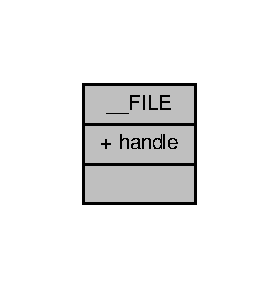
\includegraphics[width=134pt]{struct_____f_i_l_e__coll__graph}
\end{center}
\end{figure}
\subsection*{Public Attributes}
\begin{DoxyCompactItemize}
\item 
int \hyperlink{struct_____f_i_l_e_ac65d6afc3b2c74e74d56195829a1626f}{handle}
\end{DoxyCompactItemize}


\subsection{Detailed Description}


Definition at line 28 of file Retarget.\-c.



\subsection{Member Data Documentation}
\hypertarget{struct_____f_i_l_e_ac65d6afc3b2c74e74d56195829a1626f}{\index{\-\_\-\-\_\-\-F\-I\-L\-E@{\-\_\-\-\_\-\-F\-I\-L\-E}!handle@{handle}}
\index{handle@{handle}!__FILE@{\-\_\-\-\_\-\-F\-I\-L\-E}}
\subsubsection[{handle}]{\setlength{\rightskip}{0pt plus 5cm}int \-\_\-\-\_\-\-F\-I\-L\-E\-::handle}}\label{struct_____f_i_l_e_ac65d6afc3b2c74e74d56195829a1626f}


Definition at line 28 of file Retarget.\-c.



The documentation for this struct was generated from the following file\-:\begin{DoxyCompactItemize}
\item 
\hyperlink{_retarget_8c}{Retarget.\-c}\end{DoxyCompactItemize}

\hypertarget{structcommand}{\section{command Struct Reference}
\label{structcommand}\index{command@{command}}
}


{\ttfamily \#include $<$interpreter.\-h$>$}



Collaboration diagram for command\-:
\nopagebreak
\begin{figure}[H]
\begin{center}
\leavevmode
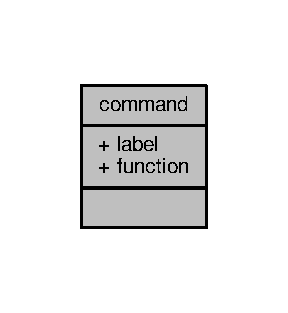
\includegraphics[width=138pt]{structcommand__coll__graph}
\end{center}
\end{figure}
\subsection*{Public Attributes}
\begin{DoxyCompactItemize}
\item 
char $\ast$ \hyperlink{structcommand_a556cd9d8b435c0017704254f3d9a3e57}{label}
\item 
int($\ast$ \hyperlink{structcommand_a217dfc1d06446ee6606a9a007fa6a7b6}{function} )(char $\ast$)
\end{DoxyCompactItemize}


\subsection{Detailed Description}


Definition at line 26 of file interpreter.\-h.



\subsection{Member Data Documentation}
\hypertarget{structcommand_a217dfc1d06446ee6606a9a007fa6a7b6}{\index{command@{command}!function@{function}}
\index{function@{function}!command@{command}}
\subsubsection[{function}]{\setlength{\rightskip}{0pt plus 5cm}int($\ast$ command\-::function)(char $\ast$)}}\label{structcommand_a217dfc1d06446ee6606a9a007fa6a7b6}


Definition at line 29 of file interpreter.\-h.

\hypertarget{structcommand_a556cd9d8b435c0017704254f3d9a3e57}{\index{command@{command}!label@{label}}
\index{label@{label}!command@{command}}
\subsubsection[{label}]{\setlength{\rightskip}{0pt plus 5cm}char$\ast$ command\-::label}}\label{structcommand_a556cd9d8b435c0017704254f3d9a3e57}


Definition at line 28 of file interpreter.\-h.



The documentation for this struct was generated from the following file\-:\begin{DoxyCompactItemize}
\item 
\hyperlink{interpreter_8h}{interpreter.\-h}\end{DoxyCompactItemize}

\chapter{File Documentation}
\hypertarget{_a_d_c_8c}{\section{A\-D\-C.\-c File Reference}
\label{_a_d_c_8c}\index{A\-D\-C.\-c@{A\-D\-C.\-c}}
}
{\ttfamily \#include \char`\"{}A\-D\-C.\-h\char`\"{}}\\*
{\ttfamily \#include $<$stdint.\-h$>$}\\*
{\ttfamily \#include \char`\"{}inc/tm4c123gh6pm.\-h\char`\"{}}\\*
Include dependency graph for A\-D\-C.\-c\-:
\nopagebreak
\begin{figure}[H]
\begin{center}
\leavevmode
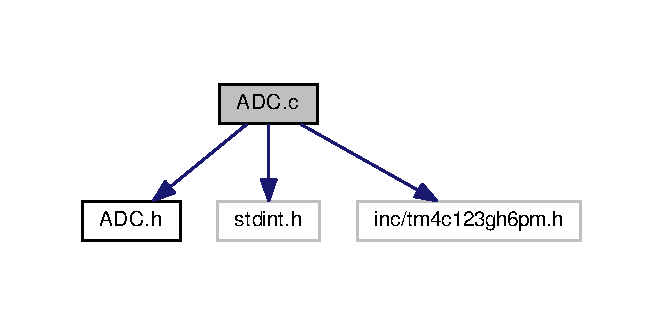
\includegraphics[width=318pt]{_a_d_c_8c__incl}
\end{center}
\end{figure}
\subsection*{Functions}
\begin{DoxyCompactItemize}
\item 
void \hyperlink{_a_d_c_8c_ac866dbaf7b167e5c46bb33de42eee84d}{Disable\-Interrupts} (void)
\item 
void \hyperlink{_a_d_c_8c_ab712356331a62b04aebcb373865e68c4}{Enable\-Interrupts} (void)
\item 
long \hyperlink{_a_d_c_8c_a6e7e2088607214bc15b17ac57b57df1b}{Start\-Critical} (void)
\item 
void \hyperlink{_a_d_c_8c_a670da3ff1aea0c7d54c40e9e40b5eeed}{End\-Critical} (long sr)
\item 
void \hyperlink{_a_d_c_8c_a80ae22f2f73496246542c428c4bec38f}{Wait\-For\-Interrupt} (void)
\item 
void \hyperlink{_a_d_c_8c_ae8d554822fd2041b8a2366ced9c0ec61}{A\-D\-C0\-Seq2\-\_\-\-Handler} (void)
\item 
void \hyperlink{_a_d_c_8c_a532438ab848632da93412a0c51c229d4}{A\-D\-C0\-Seq3\-\_\-\-Handler} (void)
\item 
void \hyperlink{_a_d_c_8c_a1a2f34caa5b32ab969b9fb7d4c0b1d6b}{A\-D\-C0\-Seq1\-\_\-\-Handler} (void)
\item 
int \hyperlink{_a_d_c_8c_ae7cef9ecd73d25c0931372d21e6be943}{A\-D\-C\-\_\-init\-\_\-channel} (int channel\-Num, unsigned int fs)
\item 
int \hyperlink{_a_d_c_8c_a9fdea7e06f4c4769ab22981dafb58477}{A\-D\-C\-\_\-\-Collect} (unsigned int channel\-Num, unsigned int fs, unsigned short \hyperlink{_lab5_8c_a9516ea594e030f96eb9483d95f1583a5}{buffer}\mbox{[}$\,$\mbox{]}, unsigned int number\-Of\-Samples)
\begin{DoxyCompactList}\small\item\em Collect a set number of samples. \end{DoxyCompactList}\item 
int \hyperlink{_a_d_c_8c_ab991147608f978ac77baf774334e802b}{A\-D\-C\-\_\-\-Status} (int id)
\begin{DoxyCompactList}\small\item\em returns 0 when A\-D\-C\-\_\-collect finishes \end{DoxyCompactList}\end{DoxyCompactItemize}
\subsection*{Variables}
\begin{DoxyCompactItemize}
\item 
volatile int \hyperlink{_a_d_c_8c_aa9e74f4242577ace4147b2205821a7a3}{Open} \mbox{[}4\mbox{]} = \{0,0,0,0\}
\item 
volatile int \hyperlink{_a_d_c_8c_a2dda4a471bcd1c89a9e099a5203dd29a}{Collecting} \mbox{[}4\mbox{]} = \{0,0,0,0\}
\item 
volatile unsigned short $\ast$ \hyperlink{_a_d_c_8c_a5a00ab78e84682ce357562e66203fbc9}{Buffer0}
\item 
volatile unsigned short $\ast$ \hyperlink{_a_d_c_8c_a5e510bf438e51a8252b7eee23ae1ba88}{Buffer1}
\item 
volatile unsigned short $\ast$ \hyperlink{_a_d_c_8c_ac4491cb99756a73234eb72f199e64cad}{Buffer2}
\item 
volatile unsigned short $\ast$ \hyperlink{_a_d_c_8c_ac4192b26a52a91f1541df9414277376c}{Buffer3}
\item 
volatile int \hyperlink{_a_d_c_8c_a1b4ccff92594e3fb8d1cc0e2cc44f685}{Sample\-Count} \mbox{[}4\mbox{]}
\item 
volatile int \hyperlink{_a_d_c_8c_a391ced11089028ee480c98537a134f63}{Target\-Count} \mbox{[}4\mbox{]}
\item 
volatile int \hyperlink{_a_d_c_8c_a63873eac54c61cd643e5dc99b411d585}{Current\-Channel}
\item 
volatile unsigned short \hyperlink{_a_d_c_8c_ac73df7e82cfb7052ed9f39ebd4fb4c3b}{dummy0}
\end{DoxyCompactItemize}


\subsection{Function Documentation}
\hypertarget{_a_d_c_8c_a1a2f34caa5b32ab969b9fb7d4c0b1d6b}{\index{A\-D\-C.\-c@{A\-D\-C.\-c}!A\-D\-C0\-Seq1\-\_\-\-Handler@{A\-D\-C0\-Seq1\-\_\-\-Handler}}
\index{A\-D\-C0\-Seq1\-\_\-\-Handler@{A\-D\-C0\-Seq1\-\_\-\-Handler}!ADC.c@{A\-D\-C.\-c}}
\subsubsection[{A\-D\-C0\-Seq1\-\_\-\-Handler}]{\setlength{\rightskip}{0pt plus 5cm}void A\-D\-C0\-Seq1\-\_\-\-Handler (
\begin{DoxyParamCaption}
\item[{void}]{}
\end{DoxyParamCaption}
)}}\label{_a_d_c_8c_a1a2f34caa5b32ab969b9fb7d4c0b1d6b}
\hypertarget{_a_d_c_8c_ae8d554822fd2041b8a2366ced9c0ec61}{\index{A\-D\-C.\-c@{A\-D\-C.\-c}!A\-D\-C0\-Seq2\-\_\-\-Handler@{A\-D\-C0\-Seq2\-\_\-\-Handler}}
\index{A\-D\-C0\-Seq2\-\_\-\-Handler@{A\-D\-C0\-Seq2\-\_\-\-Handler}!ADC.c@{A\-D\-C.\-c}}
\subsubsection[{A\-D\-C0\-Seq2\-\_\-\-Handler}]{\setlength{\rightskip}{0pt plus 5cm}void A\-D\-C0\-Seq2\-\_\-\-Handler (
\begin{DoxyParamCaption}
\item[{void}]{}
\end{DoxyParamCaption}
)}}\label{_a_d_c_8c_ae8d554822fd2041b8a2366ced9c0ec61}


Definition at line 248 of file A\-D\-C.\-c.


\begin{DoxyCode}
248                            \{
249   \textcolor{keywordflow}{if}(\hyperlink{_a_d_c_8c_a2dda4a471bcd1c89a9e099a5203dd29a}{Collecting}[\hyperlink{_a_d_c_8c_a63873eac54c61cd643e5dc99b411d585}{CurrentChannel}] > 0)\{
250     ADC0\_ISC\_R = 0x04;          \textcolor{comment}{// acknowledge ADC sequence 2 completion}
251     \hyperlink{_a_d_c_8c_a1b4ccff92594e3fb8d1cc0e2cc44f685}{SampleCount}[\hyperlink{_a_d_c_8c_a63873eac54c61cd643e5dc99b411d585}{CurrentChannel}]+=2;          \textcolor{comment}{// taking care of reducing the
       frequency by a factor 2}
252     \textcolor{keywordflow}{switch}(\hyperlink{_a_d_c_8c_a63873eac54c61cd643e5dc99b411d585}{CurrentChannel})\{
253       \textcolor{keywordflow}{case} 0: \hyperlink{_a_d_c_8c_a5a00ab78e84682ce357562e66203fbc9}{Buffer0}[\hyperlink{_a_d_c_8c_a1b4ccff92594e3fb8d1cc0e2cc44f685}{SampleCount}[0]/2] = ADC0\_SSFIFO2\_R;  
      \hyperlink{_a_d_c_8c_ac73df7e82cfb7052ed9f39ebd4fb4c3b}{dummy0} = ADC0\_SSFIFO2\_R; \textcolor{keywordflow}{break};
254       \textcolor{keywordflow}{case} 1: \hyperlink{_a_d_c_8c_a5e510bf438e51a8252b7eee23ae1ba88}{Buffer1}[SampleCount[1]/2] = ADC0\_SSFIFO2\_R;  \hyperlink{_a_d_c_8c_ac73df7e82cfb7052ed9f39ebd4fb4c3b}{dummy0} = ADC0\_SSFIFO2\_R; \textcolor{keywordflow}{break};
255       \textcolor{keywordflow}{case} 2: \hyperlink{_a_d_c_8c_ac4491cb99756a73234eb72f199e64cad}{Buffer2}[SampleCount[2]/2] = ADC0\_SSFIFO2\_R;  \hyperlink{_a_d_c_8c_ac73df7e82cfb7052ed9f39ebd4fb4c3b}{dummy0} = ADC0\_SSFIFO2\_R; \textcolor{keywordflow}{break};
256       \textcolor{keywordflow}{case} 3: \hyperlink{_a_d_c_8c_ac4192b26a52a91f1541df9414277376c}{Buffer3}[SampleCount[3]/2] = ADC0\_SSFIFO2\_R;  \hyperlink{_a_d_c_8c_ac73df7e82cfb7052ed9f39ebd4fb4c3b}{dummy0} = ADC0\_SSFIFO2\_R; \textcolor{keywordflow}{break};
257     \}
258     
259 \textcolor{comment}{//    Buffer[0][SampleCount[0]++] = ADC0\_SSFIFO2\_R;}
260     \textcolor{comment}{//TODO May need to double read to pop from fifo}
261     \hyperlink{_a_d_c_8c_a2dda4a471bcd1c89a9e099a5203dd29a}{Collecting}[\hyperlink{_a_d_c_8c_a63873eac54c61cd643e5dc99b411d585}{CurrentChannel}] = \hyperlink{_a_d_c_8c_a391ced11089028ee480c98537a134f63}{TargetCount}[
      \hyperlink{_a_d_c_8c_a63873eac54c61cd643e5dc99b411d585}{CurrentChannel}] - \hyperlink{_a_d_c_8c_a1b4ccff92594e3fb8d1cc0e2cc44f685}{SampleCount}[\hyperlink{_a_d_c_8c_a63873eac54c61cd643e5dc99b411d585}{CurrentChannel}]; \textcolor{comment}{//Faster than
       branching}
262   \}
263   \textcolor{keywordflow}{else}\{ \textcolor{comment}{//Not Collecting}
264     NVIC\_DIS0\_R = 1<<16; \textcolor{comment}{//Disable SS2 Interrupt}
265   \}
266 \}
\end{DoxyCode}
\hypertarget{_a_d_c_8c_a532438ab848632da93412a0c51c229d4}{\index{A\-D\-C.\-c@{A\-D\-C.\-c}!A\-D\-C0\-Seq3\-\_\-\-Handler@{A\-D\-C0\-Seq3\-\_\-\-Handler}}
\index{A\-D\-C0\-Seq3\-\_\-\-Handler@{A\-D\-C0\-Seq3\-\_\-\-Handler}!ADC.c@{A\-D\-C.\-c}}
\subsubsection[{A\-D\-C0\-Seq3\-\_\-\-Handler}]{\setlength{\rightskip}{0pt plus 5cm}void A\-D\-C0\-Seq3\-\_\-\-Handler (
\begin{DoxyParamCaption}
\item[{void}]{}
\end{DoxyParamCaption}
)}}\label{_a_d_c_8c_a532438ab848632da93412a0c51c229d4}
\hypertarget{_a_d_c_8c_a9fdea7e06f4c4769ab22981dafb58477}{\index{A\-D\-C.\-c@{A\-D\-C.\-c}!A\-D\-C\-\_\-\-Collect@{A\-D\-C\-\_\-\-Collect}}
\index{A\-D\-C\-\_\-\-Collect@{A\-D\-C\-\_\-\-Collect}!ADC.c@{A\-D\-C.\-c}}
\subsubsection[{A\-D\-C\-\_\-\-Collect}]{\setlength{\rightskip}{0pt plus 5cm}int A\-D\-C\-\_\-\-Collect (
\begin{DoxyParamCaption}
\item[{unsigned int}]{channel\-Num, }
\item[{unsigned int}]{fs, }
\item[{unsigned short}]{buffer\mbox{[}$\,$\mbox{]}, }
\item[{unsigned int}]{number\-Of\-Samples}
\end{DoxyParamCaption}
)}}\label{_a_d_c_8c_a9fdea7e06f4c4769ab22981dafb58477}


Collect a set number of samples. 

Collect a sequence of A\-D\-C values.

\mbox{[}long description\mbox{]}


\begin{DoxyParams}{Parameters}
{\em channel\-Num} & Channel to configure \\
\hline
{\em fs} & Sample Frequency (Hz) must be between 100\-Hz and 10k\-Hz \\
\hline
{\em buffer} & Array to buffer data, does not bounds check buffer \\
\hline
{\em number\-Of\-Samples} & number of samples to record must be even number $>$ 1 \\
\hline
\end{DoxyParams}
\begin{DoxyReturn}{Returns}
0 if initialization successful, -\/1 if fail
\end{DoxyReturn}
Uses A\-D\-C Sample Sequencer 2 and Timer 0. Does not require call to \hyperlink{_a_d_c_8h_a9b319827131872257b8c6a8658852cc0}{A\-D\-C\-\_\-\-Open()} 

Definition at line 171 of file A\-D\-C.\-c.


\begin{DoxyCode}
173 \{
174   \textcolor{keywordflow}{if}(fs < 100 || fs > 10000)\{
175     \textcolor{keywordflow}{return} -1;
176   \}
177   \textcolor{keywordflow}{if}(numberOfSamples < 1)\{
178     \textcolor{keywordflow}{return} -1;
179   \}
180   
181   \hyperlink{_a_d_c_8c_ac866dbaf7b167e5c46bb33de42eee84d}{DisableInterrupts}();
182   ADC0\_ACTSS\_R &= ~0x04;    \textcolor{comment}{// disable sample sequencer 2}
183   ADC0\_EMUX\_R = (ADC0\_EMUX\_R&0xFFFFF0FF)+0x0500; \textcolor{comment}{// timer trigger event SS2}
184 
185   ADC0\_SAC\_R = 0x02;  \textcolor{comment}{// 4x Hardware Oversample}
186  
187   ADC0\_SSMUX2\_R = (channelNum << 4) | channelNum;
188   ADC0\_SSCTL2\_R = 0x064;          \textcolor{comment}{// set flag and end, 2 samples at a time                      }
189   ADC0\_IM\_R |= 0x04;             \textcolor{comment}{// enable SS2 interrupts}
190   ADC0\_ACTSS\_R |= 0x04;          \textcolor{comment}{// enable sample sequencer 2}
191   NVIC\_PRI4\_R = (NVIC\_PRI4\_R & 0xFFFF00FF)|0x00004000; \textcolor{comment}{//priority 2}
192   NVIC\_EN0\_R = 1<<16;              \textcolor{comment}{// enable interrupt 16 in NVIC}
193                                    \textcolor{comment}{//Sample Sequencer 2}
194   \textcolor{keywordflow}{if}(channelNum == 0)\{
195     \hyperlink{_a_d_c_8c_a2dda4a471bcd1c89a9e099a5203dd29a}{Collecting}[0] = 1;
196     \hyperlink{_a_d_c_8c_a1b4ccff92594e3fb8d1cc0e2cc44f685}{SampleCount}[0] = 0;
197     \hyperlink{_a_d_c_8c_a391ced11089028ee480c98537a134f63}{TargetCount}[0] = numberOfSamples;
198     \hyperlink{_a_d_c_8c_a5a00ab78e84682ce357562e66203fbc9}{Buffer0} = \hyperlink{interpreter_8h_ab4a03da084e15d3319078d4f4a6bf3ff}{buffer};
199     \hyperlink{_a_d_c_8c_a63873eac54c61cd643e5dc99b411d585}{CurrentChannel} = 0;
200   \}
201   \textcolor{keywordflow}{if}(channelNum == 1)\{
202     \hyperlink{_a_d_c_8c_a2dda4a471bcd1c89a9e099a5203dd29a}{Collecting}[1] = 1;
203     \hyperlink{_a_d_c_8c_a1b4ccff92594e3fb8d1cc0e2cc44f685}{SampleCount}[1] = 0;
204     \hyperlink{_a_d_c_8c_a391ced11089028ee480c98537a134f63}{TargetCount}[1] = numberOfSamples;
205     \hyperlink{_a_d_c_8c_a5e510bf438e51a8252b7eee23ae1ba88}{Buffer1} = \hyperlink{interpreter_8h_ab4a03da084e15d3319078d4f4a6bf3ff}{buffer};
206     \hyperlink{_a_d_c_8c_a63873eac54c61cd643e5dc99b411d585}{CurrentChannel} = 1;
207   \}
208   \textcolor{keywordflow}{if}(channelNum == 2)\{
209     \hyperlink{_a_d_c_8c_a2dda4a471bcd1c89a9e099a5203dd29a}{Collecting}[2] = 1;
210     \hyperlink{_a_d_c_8c_a1b4ccff92594e3fb8d1cc0e2cc44f685}{SampleCount}[2] = 0;
211     \hyperlink{_a_d_c_8c_a391ced11089028ee480c98537a134f63}{TargetCount}[2] = numberOfSamples;
212     \hyperlink{_a_d_c_8c_ac4491cb99756a73234eb72f199e64cad}{Buffer2} = \hyperlink{interpreter_8h_ab4a03da084e15d3319078d4f4a6bf3ff}{buffer};
213     \hyperlink{_a_d_c_8c_a63873eac54c61cd643e5dc99b411d585}{CurrentChannel} = 2;
214   \}
215   \textcolor{keywordflow}{if}(channelNum == 4)\{
216     \hyperlink{_a_d_c_8c_a2dda4a471bcd1c89a9e099a5203dd29a}{Collecting}[3] = 1;
217     \hyperlink{_a_d_c_8c_a1b4ccff92594e3fb8d1cc0e2cc44f685}{SampleCount}[3] = 0;
218     \hyperlink{_a_d_c_8c_a391ced11089028ee480c98537a134f63}{TargetCount}[3] = numberOfSamples;
219     \hyperlink{_a_d_c_8c_ac4192b26a52a91f1541df9414277376c}{Buffer3} = \hyperlink{interpreter_8h_ab4a03da084e15d3319078d4f4a6bf3ff}{buffer};
220     \hyperlink{_a_d_c_8c_a63873eac54c61cd643e5dc99b411d585}{CurrentChannel} = 3;
221   \}
222   \hyperlink{_a_d_c_8c_ab712356331a62b04aebcb373865e68c4}{EnableInterrupts}();
223 
224   \textcolor{keywordflow}{return} \hyperlink{_a_d_c_8c_a2dda4a471bcd1c89a9e099a5203dd29a}{Collecting}[0];
225 \}
\end{DoxyCode}


Here is the call graph for this function\-:
\nopagebreak
\begin{figure}[H]
\begin{center}
\leavevmode
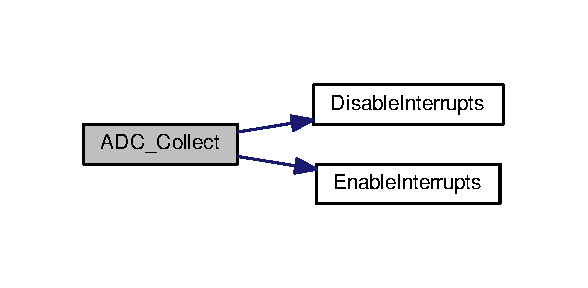
\includegraphics[width=282pt]{_a_d_c_8c_a9fdea7e06f4c4769ab22981dafb58477_cgraph}
\end{center}
\end{figure}




Here is the caller graph for this function\-:
\nopagebreak
\begin{figure}[H]
\begin{center}
\leavevmode
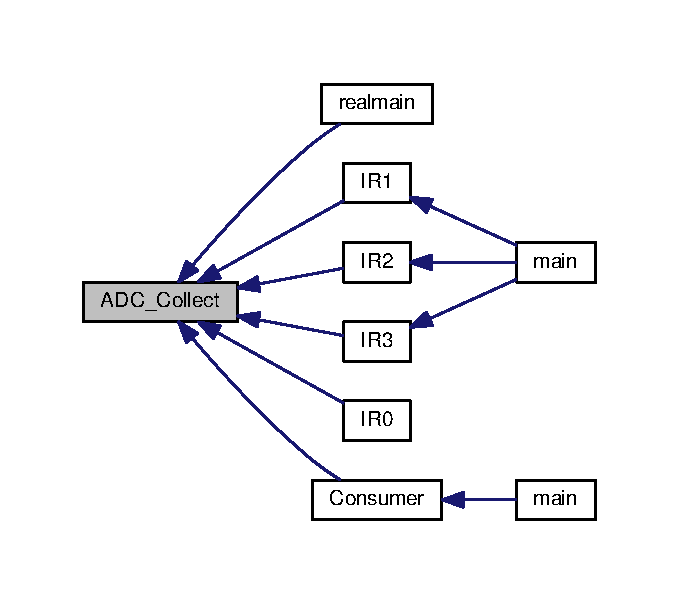
\includegraphics[width=326pt]{_a_d_c_8c_a9fdea7e06f4c4769ab22981dafb58477_icgraph}
\end{center}
\end{figure}


\hypertarget{_a_d_c_8c_ae7cef9ecd73d25c0931372d21e6be943}{\index{A\-D\-C.\-c@{A\-D\-C.\-c}!A\-D\-C\-\_\-init\-\_\-channel@{A\-D\-C\-\_\-init\-\_\-channel}}
\index{A\-D\-C\-\_\-init\-\_\-channel@{A\-D\-C\-\_\-init\-\_\-channel}!ADC.c@{A\-D\-C.\-c}}
\subsubsection[{A\-D\-C\-\_\-init\-\_\-channel}]{\setlength{\rightskip}{0pt plus 5cm}int A\-D\-C\-\_\-init\-\_\-channel (
\begin{DoxyParamCaption}
\item[{int}]{channel\-Num, }
\item[{unsigned int}]{fs}
\end{DoxyParamCaption}
)}}\label{_a_d_c_8c_ae7cef9ecd73d25c0931372d21e6be943}


Definition at line 36 of file A\-D\-C.\-c.


\begin{DoxyCode}
36                                                      \{
37   \textcolor{keyword}{volatile} uint32\_t delay;
38   \textcolor{keywordflow}{if}(fs < 100 || fs > 10000)\{
39     \textcolor{keywordflow}{return} -1;
40   \} 
41   \textcolor{comment}{// **** GPIO pin initialization ****}
42   \textcolor{keywordflow}{switch}(channelNum)\{             \textcolor{comment}{// 1) activate clock}
43     \textcolor{keywordflow}{case} 0:
44     \textcolor{keywordflow}{case} 1:
45     \textcolor{keywordflow}{case} 2:
46     \textcolor{keywordflow}{case} 3:
47     \textcolor{keywordflow}{case} 8:
48     \textcolor{keywordflow}{case} 9:                       \textcolor{comment}{//    these are on GPIO\_PORTE}
49       SYSCTL\_RCGCGPIO\_R |= SYSCTL\_RCGCGPIO\_R4; \textcolor{keywordflow}{break};
50     \textcolor{keywordflow}{case} 4:
51     \textcolor{keywordflow}{case} 5:
52     \textcolor{keywordflow}{case} 6:
53     \textcolor{keywordflow}{case} 7:                       \textcolor{comment}{// these are on GPIO\_PORTD}
54       SYSCTL\_RCGCGPIO\_R |= SYSCTL\_RCGCGPIO\_R3; \textcolor{keywordflow}{break};
55     \textcolor{keywordflow}{case} 10:
56     \textcolor{keywordflow}{case} 11:                      \textcolor{comment}{// these are on GPIO\_PORTB}
57       SYSCTL\_RCGCGPIO\_R |= SYSCTL\_RCGCGPIO\_R1; \textcolor{keywordflow}{break};
58     \textcolor{keywordflow}{default}: \textcolor{keywordflow}{return} -1;              \textcolor{comment}{//0 to 11 are valid channels on the LM4F120}
59   \}
60   delay = SYSCTL\_RCGCGPIO\_R;      \textcolor{comment}{// 2) allow time for clock to stabilize}
61   delay = SYSCTL\_RCGCGPIO\_R;
62   \textcolor{keywordflow}{switch}(channelNum)\{
63     \textcolor{keywordflow}{case} 0:                       \textcolor{comment}{//      Ain0 is on PE3}
64       GPIO\_PORTE\_DIR\_R &= ~0x08;  \textcolor{comment}{// 3.0) make PE3 input}
65       GPIO\_PORTE\_AFSEL\_R |= 0x08; \textcolor{comment}{// 4.0) enable alternate function on PE3}
66       GPIO\_PORTE\_DEN\_R &= ~0x08;  \textcolor{comment}{// 5.0) disable digital I/O on PE3}
67       GPIO\_PORTE\_AMSEL\_R |= 0x08; \textcolor{comment}{// 6.0) enable analog functionality on PE3}
68       \textcolor{keywordflow}{break};
69     \textcolor{keywordflow}{case} 1:                       \textcolor{comment}{//      Ain1 is on PE2}
70       GPIO\_PORTE\_DIR\_R &= ~0x04;  \textcolor{comment}{// 3.1) make PE2 input}
71       GPIO\_PORTE\_AFSEL\_R |= 0x04; \textcolor{comment}{// 4.1) enable alternate function on PE2}
72       GPIO\_PORTE\_DEN\_R &= ~0x04;  \textcolor{comment}{// 5.1) disable digital I/O on PE2}
73       GPIO\_PORTE\_AMSEL\_R |= 0x04; \textcolor{comment}{// 6.1) enable analog functionality on PE2}
74       \textcolor{keywordflow}{break};
75     \textcolor{keywordflow}{case} 2:                       \textcolor{comment}{//      Ain2 is on PE1}
76       GPIO\_PORTE\_DIR\_R &= ~0x02;  \textcolor{comment}{// 3.2) make PE1 input}
77       GPIO\_PORTE\_AFSEL\_R |= 0x02; \textcolor{comment}{// 4.2) enable alternate function on PE1}
78       GPIO\_PORTE\_DEN\_R &= ~0x02;  \textcolor{comment}{// 5.2) disable digital I/O on PE1}
79       GPIO\_PORTE\_AMSEL\_R |= 0x02; \textcolor{comment}{// 6.2) enable analog functionality on PE1}
80       \textcolor{keywordflow}{break};
81     \textcolor{keywordflow}{case} 3:                       \textcolor{comment}{//      Ain3 is on PE0}
82       GPIO\_PORTE\_DIR\_R &= ~0x01;  \textcolor{comment}{// 3.3) make PE0 input}
83       GPIO\_PORTE\_AFSEL\_R |= 0x01; \textcolor{comment}{// 4.3) enable alternate function on PE0}
84       GPIO\_PORTE\_DEN\_R &= ~0x01;  \textcolor{comment}{// 5.3) disable digital I/O on PE0}
85       GPIO\_PORTE\_AMSEL\_R |= 0x01; \textcolor{comment}{// 6.3) enable analog functionality on PE0}
86       \textcolor{keywordflow}{break};
87     \textcolor{keywordflow}{case} 4:                       \textcolor{comment}{//      Ain4 is on PD3}
88       GPIO\_PORTD\_DIR\_R &= ~0x08;  \textcolor{comment}{// 3.4) make PD3 input}
89       GPIO\_PORTD\_AFSEL\_R |= 0x08; \textcolor{comment}{// 4.4) enable alternate function on PD3}
90       GPIO\_PORTD\_DEN\_R &= ~0x08;  \textcolor{comment}{// 5.4) disable digital I/O on PD3}
91       GPIO\_PORTD\_AMSEL\_R |= 0x08; \textcolor{comment}{// 6.4) enable analog functionality on PD3}
92       \textcolor{keywordflow}{break};
93     \textcolor{keywordflow}{case} 5:                       \textcolor{comment}{//      Ain5 is on PD2}
94       GPIO\_PORTD\_DIR\_R &= ~0x04;  \textcolor{comment}{// 3.5) make PD2 input}
95       GPIO\_PORTD\_AFSEL\_R |= 0x04; \textcolor{comment}{// 4.5) enable alternate function on PD2}
96       GPIO\_PORTD\_DEN\_R &= ~0x04;  \textcolor{comment}{// 5.5) disable digital I/O on PD2}
97       GPIO\_PORTD\_AMSEL\_R |= 0x04; \textcolor{comment}{// 6.5) enable analog functionality on PD2}
98       \textcolor{keywordflow}{break};
99     \textcolor{keywordflow}{case} 6:                       \textcolor{comment}{//      Ain6 is on PD1}
100       GPIO\_PORTD\_DIR\_R &= ~0x02;  \textcolor{comment}{// 3.6) make PD1 input}
101       GPIO\_PORTD\_AFSEL\_R |= 0x02; \textcolor{comment}{// 4.6) enable alternate function on PD1}
102       GPIO\_PORTD\_DEN\_R &= ~0x02;  \textcolor{comment}{// 5.6) disable digital I/O on PD1}
103       GPIO\_PORTD\_AMSEL\_R |= 0x02; \textcolor{comment}{// 6.6) enable analog functionality on PD1}
104       \textcolor{keywordflow}{break};
105     \textcolor{keywordflow}{case} 7:                       \textcolor{comment}{//      Ain7 is on PD0}
106       GPIO\_PORTD\_DIR\_R &= ~0x01;  \textcolor{comment}{// 3.7) make PD0 input}
107       GPIO\_PORTD\_AFSEL\_R |= 0x01; \textcolor{comment}{// 4.7) enable alternate function on PD0}
108       GPIO\_PORTD\_DEN\_R &= ~0x01;  \textcolor{comment}{// 5.7) disable digital I/O on PD0}
109       GPIO\_PORTD\_AMSEL\_R |= 0x01; \textcolor{comment}{// 6.7) enable analog functionality on PD0}
110       \textcolor{keywordflow}{break};
111     \textcolor{keywordflow}{case} 8:                       \textcolor{comment}{//      Ain8 is on PE5}
112       GPIO\_PORTE\_DIR\_R &= ~0x20;  \textcolor{comment}{// 3.8) make PE5 input}
113       GPIO\_PORTE\_AFSEL\_R |= 0x20; \textcolor{comment}{// 4.8) enable alternate function on PE5}
114       GPIO\_PORTE\_DEN\_R &= ~0x20;  \textcolor{comment}{// 5.8) disable digital I/O on PE5}
115       GPIO\_PORTE\_AMSEL\_R |= 0x20; \textcolor{comment}{// 6.8) enable analog functionality on PE5}
116       \textcolor{keywordflow}{break};
117     \textcolor{keywordflow}{case} 9:                       \textcolor{comment}{//      Ain9 is on PE4}
118       GPIO\_PORTE\_DIR\_R &= ~0x10;  \textcolor{comment}{// 3.9) make PE4 input}
119       GPIO\_PORTE\_AFSEL\_R |= 0x10; \textcolor{comment}{// 4.9) enable alternate function on PE4}
120       GPIO\_PORTE\_DEN\_R &= ~0x10;  \textcolor{comment}{// 5.9) disable digital I/O on PE4}
121       GPIO\_PORTE\_AMSEL\_R |= 0x10; \textcolor{comment}{// 6.9) enable analog functionality on PE4}
122       \textcolor{keywordflow}{break};
123     \textcolor{keywordflow}{case} 10:                      \textcolor{comment}{//       Ain10 is on PB4}
124       GPIO\_PORTB\_DIR\_R &= ~0x10;  \textcolor{comment}{// 3.10) make PB4 input}
125       GPIO\_PORTB\_AFSEL\_R |= 0x10; \textcolor{comment}{// 4.10) enable alternate function on PB4}
126       GPIO\_PORTB\_DEN\_R &= ~0x10;  \textcolor{comment}{// 5.10) disable digital I/O on PB4}
127       GPIO\_PORTB\_AMSEL\_R |= 0x10; \textcolor{comment}{// 6.10) enable analog functionality on PB4}
128       \textcolor{keywordflow}{break};
129     \textcolor{keywordflow}{case} 11:                      \textcolor{comment}{//       Ain11 is on PB5}
130       GPIO\_PORTB\_DIR\_R &= ~0x20;  \textcolor{comment}{// 3.11) make PB5 input}
131       GPIO\_PORTB\_AFSEL\_R |= 0x20; \textcolor{comment}{// 4.11) enable alternate function on PB5}
132       GPIO\_PORTB\_DEN\_R &= ~0x20;  \textcolor{comment}{// 5.11) disable digital I/O on PB5}
133       GPIO\_PORTB\_AMSEL\_R |= 0x20; \textcolor{comment}{// 6.11) enable analog functionality on PB5}
134       \textcolor{keywordflow}{break};
135   \}
136   \hyperlink{_a_d_c_8c_ac866dbaf7b167e5c46bb33de42eee84d}{DisableInterrupts}();
137   SYSCTL\_RCGCADC\_R |= 0x01;     \textcolor{comment}{// activate ADC0 }
138   SYSCTL\_RCGCTIMER\_R |= 0x01;   \textcolor{comment}{// activate timer0 }
139   delay = SYSCTL\_RCGCTIMER\_R;   \textcolor{comment}{// allow time to finish activating}
140 
141   TIMER0\_CTL\_R = 0x00000000;    \textcolor{comment}{// disable timer0A during setup}
142   TIMER0\_CTL\_R |= 0x00000020;   \textcolor{comment}{// enable timer0A trigger to ADC}
143   TIMER0\_CFG\_R = 0;             \textcolor{comment}{// configure for 32-bit timer mode}
144   TIMER0\_TAMR\_R = 0x00000002;   \textcolor{comment}{// configure for periodic mode, default down-count settings}
145   TIMER0\_TAPR\_R = 0;            \textcolor{comment}{// prescale value for trigger}
146   TIMER0\_TAILR\_R = (80000000/fs)-1;    \textcolor{comment}{// start value for trigger}
147   TIMER0\_IMR\_R = 0x00000000;    \textcolor{comment}{// disable all interrupts}
148   TIMER0\_CTL\_R |= 0x00000001;   \textcolor{comment}{// enable timer0A 32-b, periodic, no interrupts}
149   
150   ADC0\_PC\_R = 0x01;         \textcolor{comment}{// configure for 125K samples/sec}
151   ADC0\_SSPRI\_R = 0x3210;    \textcolor{comment}{// sequencer 0 is highest, sequencer 3 is lowest}
152   \hyperlink{_a_d_c_8c_ab712356331a62b04aebcb373865e68c4}{EnableInterrupts}();
153   \textcolor{keywordflow}{return} 1;
154 \}
\end{DoxyCode}


Here is the call graph for this function\-:
\nopagebreak
\begin{figure}[H]
\begin{center}
\leavevmode
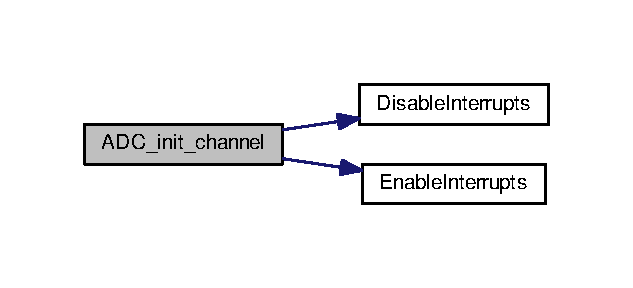
\includegraphics[width=304pt]{_a_d_c_8c_ae7cef9ecd73d25c0931372d21e6be943_cgraph}
\end{center}
\end{figure}




Here is the caller graph for this function\-:
\nopagebreak
\begin{figure}[H]
\begin{center}
\leavevmode
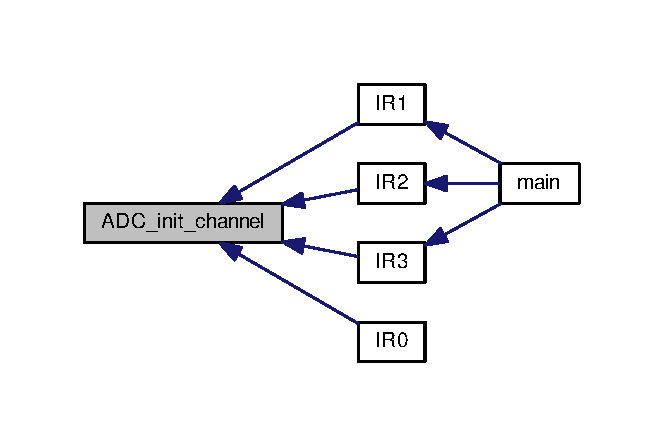
\includegraphics[width=318pt]{_a_d_c_8c_ae7cef9ecd73d25c0931372d21e6be943_icgraph}
\end{center}
\end{figure}


\hypertarget{_a_d_c_8c_ab991147608f978ac77baf774334e802b}{\index{A\-D\-C.\-c@{A\-D\-C.\-c}!A\-D\-C\-\_\-\-Status@{A\-D\-C\-\_\-\-Status}}
\index{A\-D\-C\-\_\-\-Status@{A\-D\-C\-\_\-\-Status}!ADC.c@{A\-D\-C.\-c}}
\subsubsection[{A\-D\-C\-\_\-\-Status}]{\setlength{\rightskip}{0pt plus 5cm}int A\-D\-C\-\_\-\-Status (
\begin{DoxyParamCaption}
\item[{int}]{id}
\end{DoxyParamCaption}
)}}\label{_a_d_c_8c_ab991147608f978ac77baf774334e802b}


returns 0 when A\-D\-C\-\_\-collect finishes 

\begin{DoxyReturn}{Returns}
0 if A\-D\-C\-\_\-collect is complete, else value is the Target\-Count -\/ current Sample\-Count
\end{DoxyReturn}
Acknowledges completion at beginning of handler to minimize sample jitter. since max sample rate is 10\-K\-Hz = 100us at 80\-M\-Hz system clock, I\-S\-R likely to be relatively short. 

Definition at line 237 of file A\-D\-C.\-c.


\begin{DoxyCode}
238 \{
239   \textcolor{keywordflow}{switch}(\textcolor{keywordtype}{id})\{
240     \textcolor{keywordflow}{case} 0: \textcolor{keywordflow}{return} \hyperlink{_a_d_c_8c_a2dda4a471bcd1c89a9e099a5203dd29a}{Collecting}[0]; \textcolor{keywordflow}{break};
241     \textcolor{keywordflow}{case} 1: \textcolor{keywordflow}{return} \hyperlink{_a_d_c_8c_a2dda4a471bcd1c89a9e099a5203dd29a}{Collecting}[1]; \textcolor{keywordflow}{break};
242     \textcolor{keywordflow}{case} 2: \textcolor{keywordflow}{return} \hyperlink{_a_d_c_8c_a2dda4a471bcd1c89a9e099a5203dd29a}{Collecting}[2]; \textcolor{keywordflow}{break};
243     \textcolor{keywordflow}{case} 3: \textcolor{keywordflow}{return} \hyperlink{_a_d_c_8c_a2dda4a471bcd1c89a9e099a5203dd29a}{Collecting}[3]; \textcolor{keywordflow}{break};
244   \}
245 \}
\end{DoxyCode}


Here is the caller graph for this function\-:
\nopagebreak
\begin{figure}[H]
\begin{center}
\leavevmode
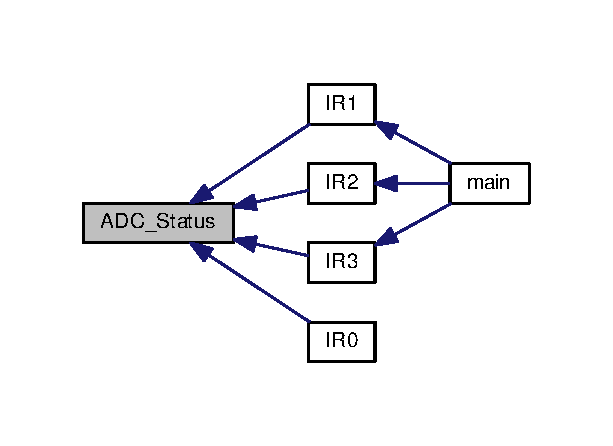
\includegraphics[width=294pt]{_a_d_c_8c_ab991147608f978ac77baf774334e802b_icgraph}
\end{center}
\end{figure}


\hypertarget{_a_d_c_8c_ac866dbaf7b167e5c46bb33de42eee84d}{\index{A\-D\-C.\-c@{A\-D\-C.\-c}!Disable\-Interrupts@{Disable\-Interrupts}}
\index{Disable\-Interrupts@{Disable\-Interrupts}!ADC.c@{A\-D\-C.\-c}}
\subsubsection[{Disable\-Interrupts}]{\setlength{\rightskip}{0pt plus 5cm}void Disable\-Interrupts (
\begin{DoxyParamCaption}
\item[{void}]{}
\end{DoxyParamCaption}
)}}\label{_a_d_c_8c_ac866dbaf7b167e5c46bb33de42eee84d}


Here is the caller graph for this function\-:
\nopagebreak
\begin{figure}[H]
\begin{center}
\leavevmode
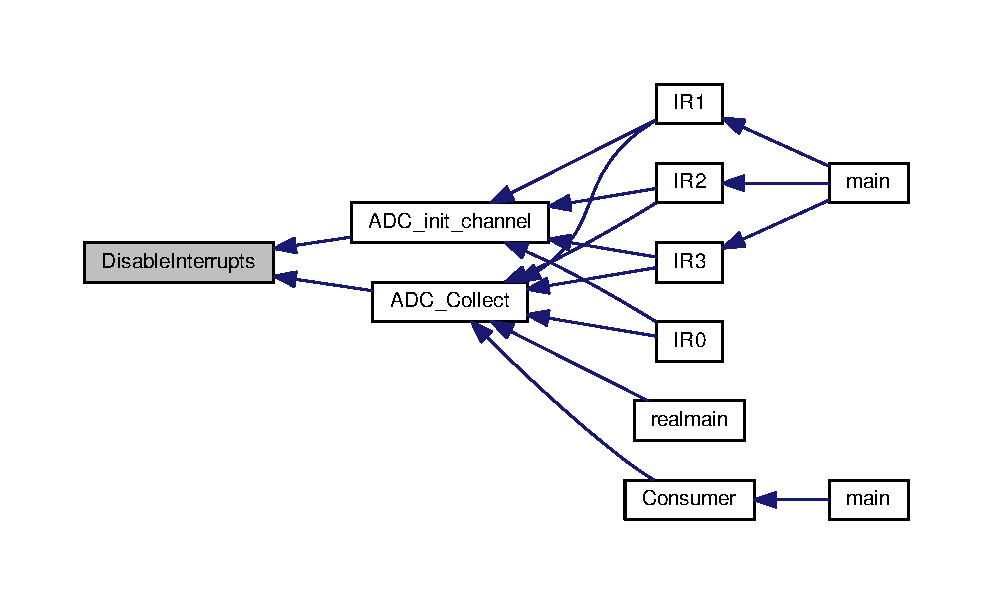
\includegraphics[width=350pt]{_a_d_c_8c_ac866dbaf7b167e5c46bb33de42eee84d_icgraph}
\end{center}
\end{figure}


\hypertarget{_a_d_c_8c_ab712356331a62b04aebcb373865e68c4}{\index{A\-D\-C.\-c@{A\-D\-C.\-c}!Enable\-Interrupts@{Enable\-Interrupts}}
\index{Enable\-Interrupts@{Enable\-Interrupts}!ADC.c@{A\-D\-C.\-c}}
\subsubsection[{Enable\-Interrupts}]{\setlength{\rightskip}{0pt plus 5cm}void Enable\-Interrupts (
\begin{DoxyParamCaption}
\item[{void}]{}
\end{DoxyParamCaption}
)}}\label{_a_d_c_8c_ab712356331a62b04aebcb373865e68c4}


Here is the caller graph for this function\-:
\nopagebreak
\begin{figure}[H]
\begin{center}
\leavevmode
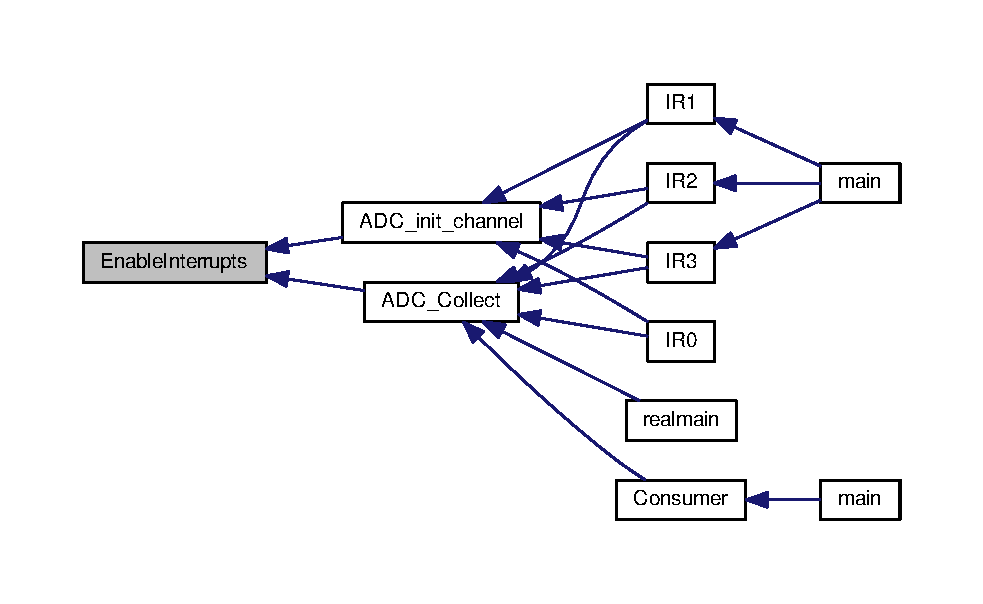
\includegraphics[width=350pt]{_a_d_c_8c_ab712356331a62b04aebcb373865e68c4_icgraph}
\end{center}
\end{figure}


\hypertarget{_a_d_c_8c_a670da3ff1aea0c7d54c40e9e40b5eeed}{\index{A\-D\-C.\-c@{A\-D\-C.\-c}!End\-Critical@{End\-Critical}}
\index{End\-Critical@{End\-Critical}!ADC.c@{A\-D\-C.\-c}}
\subsubsection[{End\-Critical}]{\setlength{\rightskip}{0pt plus 5cm}void End\-Critical (
\begin{DoxyParamCaption}
\item[{long}]{sr}
\end{DoxyParamCaption}
)}}\label{_a_d_c_8c_a670da3ff1aea0c7d54c40e9e40b5eeed}
\hypertarget{_a_d_c_8c_a6e7e2088607214bc15b17ac57b57df1b}{\index{A\-D\-C.\-c@{A\-D\-C.\-c}!Start\-Critical@{Start\-Critical}}
\index{Start\-Critical@{Start\-Critical}!ADC.c@{A\-D\-C.\-c}}
\subsubsection[{Start\-Critical}]{\setlength{\rightskip}{0pt plus 5cm}long Start\-Critical (
\begin{DoxyParamCaption}
\item[{void}]{}
\end{DoxyParamCaption}
)}}\label{_a_d_c_8c_a6e7e2088607214bc15b17ac57b57df1b}
\hypertarget{_a_d_c_8c_a80ae22f2f73496246542c428c4bec38f}{\index{A\-D\-C.\-c@{A\-D\-C.\-c}!Wait\-For\-Interrupt@{Wait\-For\-Interrupt}}
\index{Wait\-For\-Interrupt@{Wait\-For\-Interrupt}!ADC.c@{A\-D\-C.\-c}}
\subsubsection[{Wait\-For\-Interrupt}]{\setlength{\rightskip}{0pt plus 5cm}void Wait\-For\-Interrupt (
\begin{DoxyParamCaption}
\item[{void}]{}
\end{DoxyParamCaption}
)}}\label{_a_d_c_8c_a80ae22f2f73496246542c428c4bec38f}


\subsection{Variable Documentation}
\hypertarget{_a_d_c_8c_a5a00ab78e84682ce357562e66203fbc9}{\index{A\-D\-C.\-c@{A\-D\-C.\-c}!Buffer0@{Buffer0}}
\index{Buffer0@{Buffer0}!ADC.c@{A\-D\-C.\-c}}
\subsubsection[{Buffer0}]{\setlength{\rightskip}{0pt plus 5cm}volatile unsigned short$\ast$ Buffer0}}\label{_a_d_c_8c_a5a00ab78e84682ce357562e66203fbc9}


Definition at line 31 of file A\-D\-C.\-c.

\hypertarget{_a_d_c_8c_a5e510bf438e51a8252b7eee23ae1ba88}{\index{A\-D\-C.\-c@{A\-D\-C.\-c}!Buffer1@{Buffer1}}
\index{Buffer1@{Buffer1}!ADC.c@{A\-D\-C.\-c}}
\subsubsection[{Buffer1}]{\setlength{\rightskip}{0pt plus 5cm}volatile unsigned short $\ast$ Buffer1}}\label{_a_d_c_8c_a5e510bf438e51a8252b7eee23ae1ba88}


Definition at line 31 of file A\-D\-C.\-c.

\hypertarget{_a_d_c_8c_ac4491cb99756a73234eb72f199e64cad}{\index{A\-D\-C.\-c@{A\-D\-C.\-c}!Buffer2@{Buffer2}}
\index{Buffer2@{Buffer2}!ADC.c@{A\-D\-C.\-c}}
\subsubsection[{Buffer2}]{\setlength{\rightskip}{0pt plus 5cm}volatile unsigned short $\ast$ Buffer2}}\label{_a_d_c_8c_ac4491cb99756a73234eb72f199e64cad}


Definition at line 31 of file A\-D\-C.\-c.

\hypertarget{_a_d_c_8c_ac4192b26a52a91f1541df9414277376c}{\index{A\-D\-C.\-c@{A\-D\-C.\-c}!Buffer3@{Buffer3}}
\index{Buffer3@{Buffer3}!ADC.c@{A\-D\-C.\-c}}
\subsubsection[{Buffer3}]{\setlength{\rightskip}{0pt plus 5cm}volatile unsigned short $\ast$ Buffer3}}\label{_a_d_c_8c_ac4192b26a52a91f1541df9414277376c}


Definition at line 31 of file A\-D\-C.\-c.

\hypertarget{_a_d_c_8c_a2dda4a471bcd1c89a9e099a5203dd29a}{\index{A\-D\-C.\-c@{A\-D\-C.\-c}!Collecting@{Collecting}}
\index{Collecting@{Collecting}!ADC.c@{A\-D\-C.\-c}}
\subsubsection[{Collecting}]{\setlength{\rightskip}{0pt plus 5cm}volatile int Collecting\mbox{[}4\mbox{]} = \{0,0,0,0\}}}\label{_a_d_c_8c_a2dda4a471bcd1c89a9e099a5203dd29a}


Definition at line 30 of file A\-D\-C.\-c.

\hypertarget{_a_d_c_8c_a63873eac54c61cd643e5dc99b411d585}{\index{A\-D\-C.\-c@{A\-D\-C.\-c}!Current\-Channel@{Current\-Channel}}
\index{Current\-Channel@{Current\-Channel}!ADC.c@{A\-D\-C.\-c}}
\subsubsection[{Current\-Channel}]{\setlength{\rightskip}{0pt plus 5cm}volatile int Current\-Channel}}\label{_a_d_c_8c_a63873eac54c61cd643e5dc99b411d585}


Definition at line 34 of file A\-D\-C.\-c.

\hypertarget{_a_d_c_8c_ac73df7e82cfb7052ed9f39ebd4fb4c3b}{\index{A\-D\-C.\-c@{A\-D\-C.\-c}!dummy0@{dummy0}}
\index{dummy0@{dummy0}!ADC.c@{A\-D\-C.\-c}}
\subsubsection[{dummy0}]{\setlength{\rightskip}{0pt plus 5cm}volatile unsigned short dummy0}}\label{_a_d_c_8c_ac73df7e82cfb7052ed9f39ebd4fb4c3b}


Definition at line 247 of file A\-D\-C.\-c.

\hypertarget{_a_d_c_8c_aa9e74f4242577ace4147b2205821a7a3}{\index{A\-D\-C.\-c@{A\-D\-C.\-c}!Open@{Open}}
\index{Open@{Open}!ADC.c@{A\-D\-C.\-c}}
\subsubsection[{Open}]{\setlength{\rightskip}{0pt plus 5cm}volatile int Open\mbox{[}4\mbox{]} = \{0,0,0,0\}}}\label{_a_d_c_8c_aa9e74f4242577ace4147b2205821a7a3}


Definition at line 29 of file A\-D\-C.\-c.

\hypertarget{_a_d_c_8c_a1b4ccff92594e3fb8d1cc0e2cc44f685}{\index{A\-D\-C.\-c@{A\-D\-C.\-c}!Sample\-Count@{Sample\-Count}}
\index{Sample\-Count@{Sample\-Count}!ADC.c@{A\-D\-C.\-c}}
\subsubsection[{Sample\-Count}]{\setlength{\rightskip}{0pt plus 5cm}volatile int Sample\-Count\mbox{[}4\mbox{]}}}\label{_a_d_c_8c_a1b4ccff92594e3fb8d1cc0e2cc44f685}


Definition at line 32 of file A\-D\-C.\-c.

\hypertarget{_a_d_c_8c_a391ced11089028ee480c98537a134f63}{\index{A\-D\-C.\-c@{A\-D\-C.\-c}!Target\-Count@{Target\-Count}}
\index{Target\-Count@{Target\-Count}!ADC.c@{A\-D\-C.\-c}}
\subsubsection[{Target\-Count}]{\setlength{\rightskip}{0pt plus 5cm}volatile int Target\-Count\mbox{[}4\mbox{]}}}\label{_a_d_c_8c_a391ced11089028ee480c98537a134f63}


Definition at line 33 of file A\-D\-C.\-c.


\hypertarget{_a_d_c_8h}{\section{A\-D\-C.\-h File Reference}
\label{_a_d_c_8h}\index{A\-D\-C.\-h@{A\-D\-C.\-h}}
}
This graph shows which files directly or indirectly include this file\-:
\nopagebreak
\begin{figure}[H]
\begin{center}
\leavevmode
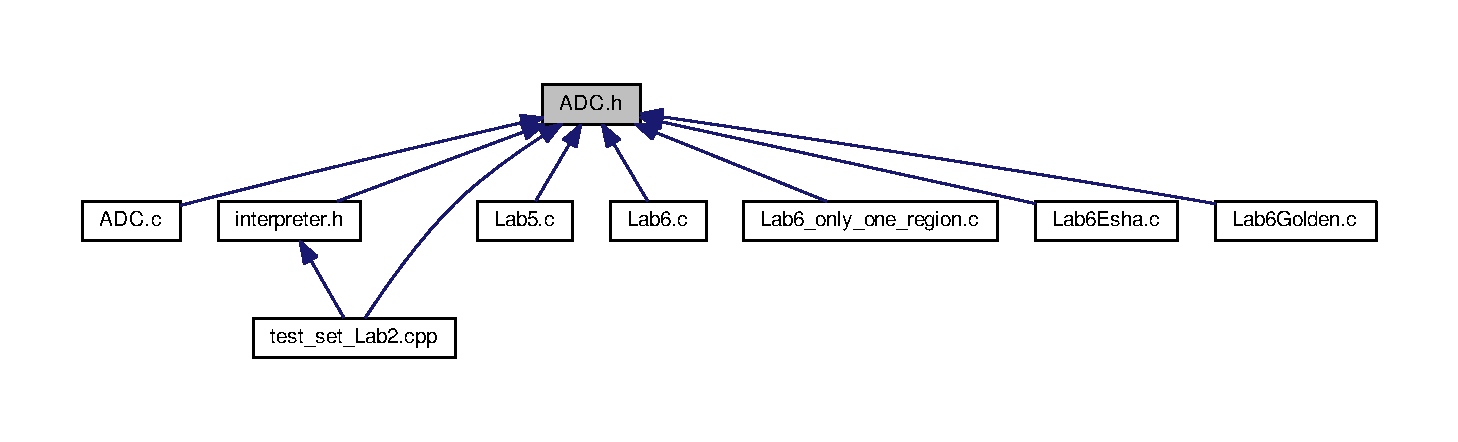
\includegraphics[width=350pt]{_a_d_c_8h__dep__incl}
\end{center}
\end{figure}
\subsection*{Functions}
\begin{DoxyCompactItemize}
\item 
int \hyperlink{_a_d_c_8h_a9b319827131872257b8c6a8658852cc0}{A\-D\-C\-\_\-\-Open} (unsigned int channel\-Num)
\begin{DoxyCompactList}\small\item\em Set up A\-D\-C on specified channel number. \end{DoxyCompactList}\item 
unsigned short \hyperlink{_a_d_c_8h_a525c5b6cd9976e6405f0bb48cee3ed51}{A\-D\-C\-\_\-\-In} (void)
\begin{DoxyCompactList}\small\item\em A\-D\-C\-\_\-\-In gets one sample from the current A\-D\-C driver. \end{DoxyCompactList}\item 
int \hyperlink{_a_d_c_8h_a9fdea7e06f4c4769ab22981dafb58477}{A\-D\-C\-\_\-\-Collect} (unsigned int channel\-Num, unsigned int fs, unsigned short \hyperlink{_lab5_8c_a9516ea594e030f96eb9483d95f1583a5}{buffer}\mbox{[}$\,$\mbox{]}, unsigned int number\-Of\-Samples)
\begin{DoxyCompactList}\small\item\em Collect a sequence of A\-D\-C values. \end{DoxyCompactList}\item 
int \hyperlink{_a_d_c_8h_ae7cef9ecd73d25c0931372d21e6be943}{A\-D\-C\-\_\-init\-\_\-channel} (int channel\-Num, unsigned int fs)
\item 
int \hyperlink{_a_d_c_8h_a2d0e1be314e7fa00367a329d13e5bbf7}{A\-D\-C\-\_\-\-Status} (int)
\begin{DoxyCompactList}\small\item\em returns 0 when A\-D\-C\-\_\-collect finishes \end{DoxyCompactList}\end{DoxyCompactItemize}


\subsection{Function Documentation}
\hypertarget{_a_d_c_8h_a9fdea7e06f4c4769ab22981dafb58477}{\index{A\-D\-C.\-h@{A\-D\-C.\-h}!A\-D\-C\-\_\-\-Collect@{A\-D\-C\-\_\-\-Collect}}
\index{A\-D\-C\-\_\-\-Collect@{A\-D\-C\-\_\-\-Collect}!ADC.h@{A\-D\-C.\-h}}
\subsubsection[{A\-D\-C\-\_\-\-Collect}]{\setlength{\rightskip}{0pt plus 5cm}int A\-D\-C\-\_\-\-Collect (
\begin{DoxyParamCaption}
\item[{unsigned int}]{channel\-Num, }
\item[{unsigned int}]{fs, }
\item[{unsigned short}]{buffer\mbox{[}$\,$\mbox{]}, }
\item[{unsigned int}]{number\-Of\-Samples}
\end{DoxyParamCaption}
)}}\label{_a_d_c_8h_a9fdea7e06f4c4769ab22981dafb58477}


Collect a sequence of A\-D\-C values. 


\begin{DoxyParams}{Parameters}
{\em channel\-Num} & Channel to configure \\
\hline
{\em fs} & Sample Frequency (Hz) between 100 and 10k\-Hz \\
\hline
{\em buffer} & Array to buffer data, does not bounds check buffer \\
\hline
{\em number\-Of\-Samples} & number of samples to record must be even (multiple of two) \\
\hline
\end{DoxyParams}
\begin{DoxyReturn}{Returns}
1 if initialization successful
\end{DoxyReturn}
To be safe, buffer must be global buffer

Collect a sequence of A\-D\-C values.

\mbox{[}long description\mbox{]}


\begin{DoxyParams}{Parameters}
{\em channel\-Num} & Channel to configure \\
\hline
{\em fs} & Sample Frequency (Hz) must be between 100\-Hz and 10k\-Hz \\
\hline
{\em buffer} & Array to buffer data, does not bounds check buffer \\
\hline
{\em number\-Of\-Samples} & number of samples to record must be even number $>$ 1 \\
\hline
\end{DoxyParams}
\begin{DoxyReturn}{Returns}
0 if initialization successful, -\/1 if fail
\end{DoxyReturn}
Uses A\-D\-C Sample Sequencer 2 and Timer 0. Does not require call to \hyperlink{_a_d_c_8h_a9b319827131872257b8c6a8658852cc0}{A\-D\-C\-\_\-\-Open()} 

Definition at line 171 of file A\-D\-C.\-c.


\begin{DoxyCode}
173 \{
174   \textcolor{keywordflow}{if}(fs < 100 || fs > 10000)\{
175     \textcolor{keywordflow}{return} -1;
176   \}
177   \textcolor{keywordflow}{if}(numberOfSamples < 1)\{
178     \textcolor{keywordflow}{return} -1;
179   \}
180   
181   \hyperlink{_a_d_c_8c_ac866dbaf7b167e5c46bb33de42eee84d}{DisableInterrupts}();
182   ADC0\_ACTSS\_R &= ~0x04;    \textcolor{comment}{// disable sample sequencer 2}
183   ADC0\_EMUX\_R = (ADC0\_EMUX\_R&0xFFFFF0FF)+0x0500; \textcolor{comment}{// timer trigger event SS2}
184 
185   ADC0\_SAC\_R = 0x02;  \textcolor{comment}{// 4x Hardware Oversample}
186  
187   ADC0\_SSMUX2\_R = (channelNum << 4) | channelNum;
188   ADC0\_SSCTL2\_R = 0x064;          \textcolor{comment}{// set flag and end, 2 samples at a time                      }
189   ADC0\_IM\_R |= 0x04;             \textcolor{comment}{// enable SS2 interrupts}
190   ADC0\_ACTSS\_R |= 0x04;          \textcolor{comment}{// enable sample sequencer 2}
191   NVIC\_PRI4\_R = (NVIC\_PRI4\_R & 0xFFFF00FF)|0x00004000; \textcolor{comment}{//priority 2}
192   NVIC\_EN0\_R = 1<<16;              \textcolor{comment}{// enable interrupt 16 in NVIC}
193                                    \textcolor{comment}{//Sample Sequencer 2}
194   \textcolor{keywordflow}{if}(channelNum == 0)\{
195     \hyperlink{_a_d_c_8c_a2dda4a471bcd1c89a9e099a5203dd29a}{Collecting}[0] = 1;
196     \hyperlink{_a_d_c_8c_a1b4ccff92594e3fb8d1cc0e2cc44f685}{SampleCount}[0] = 0;
197     \hyperlink{_a_d_c_8c_a391ced11089028ee480c98537a134f63}{TargetCount}[0] = numberOfSamples;
198     \hyperlink{_a_d_c_8c_a5a00ab78e84682ce357562e66203fbc9}{Buffer0} = \hyperlink{interpreter_8h_ab4a03da084e15d3319078d4f4a6bf3ff}{buffer};
199     \hyperlink{_a_d_c_8c_a63873eac54c61cd643e5dc99b411d585}{CurrentChannel} = 0;
200   \}
201   \textcolor{keywordflow}{if}(channelNum == 1)\{
202     \hyperlink{_a_d_c_8c_a2dda4a471bcd1c89a9e099a5203dd29a}{Collecting}[1] = 1;
203     \hyperlink{_a_d_c_8c_a1b4ccff92594e3fb8d1cc0e2cc44f685}{SampleCount}[1] = 0;
204     \hyperlink{_a_d_c_8c_a391ced11089028ee480c98537a134f63}{TargetCount}[1] = numberOfSamples;
205     \hyperlink{_a_d_c_8c_a5e510bf438e51a8252b7eee23ae1ba88}{Buffer1} = \hyperlink{interpreter_8h_ab4a03da084e15d3319078d4f4a6bf3ff}{buffer};
206     \hyperlink{_a_d_c_8c_a63873eac54c61cd643e5dc99b411d585}{CurrentChannel} = 1;
207   \}
208   \textcolor{keywordflow}{if}(channelNum == 2)\{
209     \hyperlink{_a_d_c_8c_a2dda4a471bcd1c89a9e099a5203dd29a}{Collecting}[2] = 1;
210     \hyperlink{_a_d_c_8c_a1b4ccff92594e3fb8d1cc0e2cc44f685}{SampleCount}[2] = 0;
211     \hyperlink{_a_d_c_8c_a391ced11089028ee480c98537a134f63}{TargetCount}[2] = numberOfSamples;
212     \hyperlink{_a_d_c_8c_ac4491cb99756a73234eb72f199e64cad}{Buffer2} = \hyperlink{interpreter_8h_ab4a03da084e15d3319078d4f4a6bf3ff}{buffer};
213     \hyperlink{_a_d_c_8c_a63873eac54c61cd643e5dc99b411d585}{CurrentChannel} = 2;
214   \}
215   \textcolor{keywordflow}{if}(channelNum == 4)\{
216     \hyperlink{_a_d_c_8c_a2dda4a471bcd1c89a9e099a5203dd29a}{Collecting}[3] = 1;
217     \hyperlink{_a_d_c_8c_a1b4ccff92594e3fb8d1cc0e2cc44f685}{SampleCount}[3] = 0;
218     \hyperlink{_a_d_c_8c_a391ced11089028ee480c98537a134f63}{TargetCount}[3] = numberOfSamples;
219     \hyperlink{_a_d_c_8c_ac4192b26a52a91f1541df9414277376c}{Buffer3} = \hyperlink{interpreter_8h_ab4a03da084e15d3319078d4f4a6bf3ff}{buffer};
220     \hyperlink{_a_d_c_8c_a63873eac54c61cd643e5dc99b411d585}{CurrentChannel} = 3;
221   \}
222   \hyperlink{_a_d_c_8c_ab712356331a62b04aebcb373865e68c4}{EnableInterrupts}();
223 
224   \textcolor{keywordflow}{return} \hyperlink{_a_d_c_8c_a2dda4a471bcd1c89a9e099a5203dd29a}{Collecting}[0];
225 \}
\end{DoxyCode}


Here is the call graph for this function\-:
\nopagebreak
\begin{figure}[H]
\begin{center}
\leavevmode
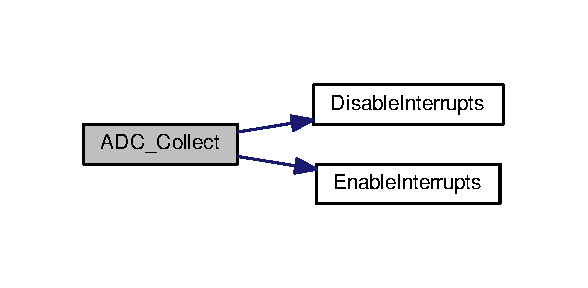
\includegraphics[width=282pt]{_a_d_c_8h_a9fdea7e06f4c4769ab22981dafb58477_cgraph}
\end{center}
\end{figure}




Here is the caller graph for this function\-:
\nopagebreak
\begin{figure}[H]
\begin{center}
\leavevmode
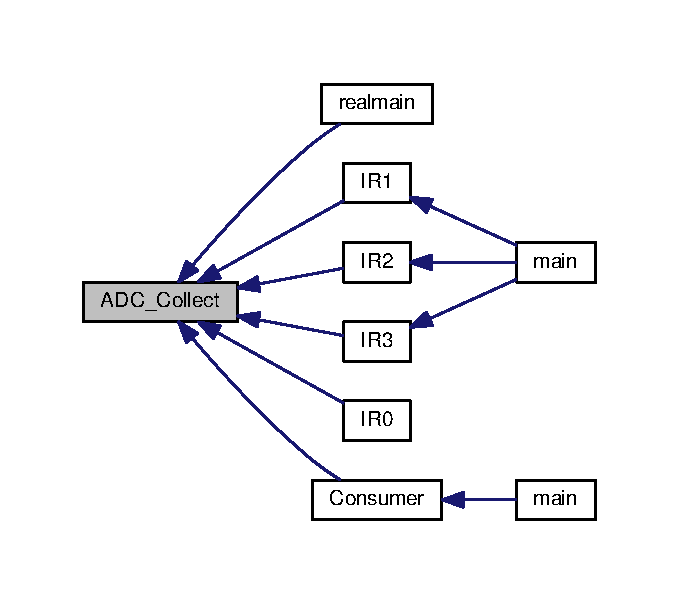
\includegraphics[width=326pt]{_a_d_c_8h_a9fdea7e06f4c4769ab22981dafb58477_icgraph}
\end{center}
\end{figure}


\hypertarget{_a_d_c_8h_a525c5b6cd9976e6405f0bb48cee3ed51}{\index{A\-D\-C.\-h@{A\-D\-C.\-h}!A\-D\-C\-\_\-\-In@{A\-D\-C\-\_\-\-In}}
\index{A\-D\-C\-\_\-\-In@{A\-D\-C\-\_\-\-In}!ADC.h@{A\-D\-C.\-h}}
\subsubsection[{A\-D\-C\-\_\-\-In}]{\setlength{\rightskip}{0pt plus 5cm}unsigned short A\-D\-C\-\_\-\-In (
\begin{DoxyParamCaption}
\item[{void}]{}
\end{DoxyParamCaption}
)}}\label{_a_d_c_8h_a525c5b6cd9976e6405f0bb48cee3ed51}


A\-D\-C\-\_\-\-In gets one sample from the current A\-D\-C driver. 

Retrieve a 10 bit scaled value from the A\-D\-C driver Must run A\-D\-C\-\_\-\-Open before calling A\-D\-C\-\_\-\-In, else returns error codes \begin{DoxyReturn}{Returns}
10 bit scaled sample from configured A\-D\-C. Error Codes are indicated by masking with 0x\-F\-C00. 0x\-F\-C00 denotes device not initialized. Other error codes are reserved. 
\end{DoxyReturn}


Here is the caller graph for this function\-:
\nopagebreak
\begin{figure}[H]
\begin{center}
\leavevmode
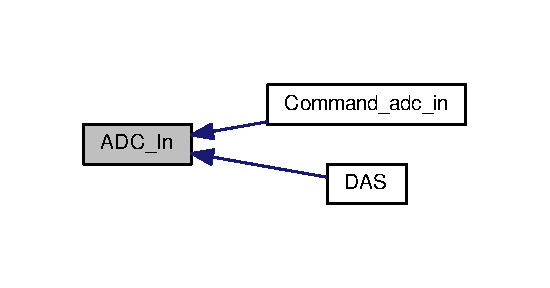
\includegraphics[width=264pt]{_a_d_c_8h_a525c5b6cd9976e6405f0bb48cee3ed51_icgraph}
\end{center}
\end{figure}


\hypertarget{_a_d_c_8h_ae7cef9ecd73d25c0931372d21e6be943}{\index{A\-D\-C.\-h@{A\-D\-C.\-h}!A\-D\-C\-\_\-init\-\_\-channel@{A\-D\-C\-\_\-init\-\_\-channel}}
\index{A\-D\-C\-\_\-init\-\_\-channel@{A\-D\-C\-\_\-init\-\_\-channel}!ADC.h@{A\-D\-C.\-h}}
\subsubsection[{A\-D\-C\-\_\-init\-\_\-channel}]{\setlength{\rightskip}{0pt plus 5cm}int A\-D\-C\-\_\-init\-\_\-channel (
\begin{DoxyParamCaption}
\item[{int}]{channel\-Num, }
\item[{unsigned int}]{fs}
\end{DoxyParamCaption}
)}}\label{_a_d_c_8h_ae7cef9ecd73d25c0931372d21e6be943}


Definition at line 36 of file A\-D\-C.\-c.


\begin{DoxyCode}
36                                                      \{
37   \textcolor{keyword}{volatile} uint32\_t delay;
38   \textcolor{keywordflow}{if}(fs < 100 || fs > 10000)\{
39     \textcolor{keywordflow}{return} -1;
40   \} 
41   \textcolor{comment}{// **** GPIO pin initialization ****}
42   \textcolor{keywordflow}{switch}(channelNum)\{             \textcolor{comment}{// 1) activate clock}
43     \textcolor{keywordflow}{case} 0:
44     \textcolor{keywordflow}{case} 1:
45     \textcolor{keywordflow}{case} 2:
46     \textcolor{keywordflow}{case} 3:
47     \textcolor{keywordflow}{case} 8:
48     \textcolor{keywordflow}{case} 9:                       \textcolor{comment}{//    these are on GPIO\_PORTE}
49       SYSCTL\_RCGCGPIO\_R |= SYSCTL\_RCGCGPIO\_R4; \textcolor{keywordflow}{break};
50     \textcolor{keywordflow}{case} 4:
51     \textcolor{keywordflow}{case} 5:
52     \textcolor{keywordflow}{case} 6:
53     \textcolor{keywordflow}{case} 7:                       \textcolor{comment}{// these are on GPIO\_PORTD}
54       SYSCTL\_RCGCGPIO\_R |= SYSCTL\_RCGCGPIO\_R3; \textcolor{keywordflow}{break};
55     \textcolor{keywordflow}{case} 10:
56     \textcolor{keywordflow}{case} 11:                      \textcolor{comment}{// these are on GPIO\_PORTB}
57       SYSCTL\_RCGCGPIO\_R |= SYSCTL\_RCGCGPIO\_R1; \textcolor{keywordflow}{break};
58     \textcolor{keywordflow}{default}: \textcolor{keywordflow}{return} -1;              \textcolor{comment}{//0 to 11 are valid channels on the LM4F120}
59   \}
60   delay = SYSCTL\_RCGCGPIO\_R;      \textcolor{comment}{// 2) allow time for clock to stabilize}
61   delay = SYSCTL\_RCGCGPIO\_R;
62   \textcolor{keywordflow}{switch}(channelNum)\{
63     \textcolor{keywordflow}{case} 0:                       \textcolor{comment}{//      Ain0 is on PE3}
64       GPIO\_PORTE\_DIR\_R &= ~0x08;  \textcolor{comment}{// 3.0) make PE3 input}
65       GPIO\_PORTE\_AFSEL\_R |= 0x08; \textcolor{comment}{// 4.0) enable alternate function on PE3}
66       GPIO\_PORTE\_DEN\_R &= ~0x08;  \textcolor{comment}{// 5.0) disable digital I/O on PE3}
67       GPIO\_PORTE\_AMSEL\_R |= 0x08; \textcolor{comment}{// 6.0) enable analog functionality on PE3}
68       \textcolor{keywordflow}{break};
69     \textcolor{keywordflow}{case} 1:                       \textcolor{comment}{//      Ain1 is on PE2}
70       GPIO\_PORTE\_DIR\_R &= ~0x04;  \textcolor{comment}{// 3.1) make PE2 input}
71       GPIO\_PORTE\_AFSEL\_R |= 0x04; \textcolor{comment}{// 4.1) enable alternate function on PE2}
72       GPIO\_PORTE\_DEN\_R &= ~0x04;  \textcolor{comment}{// 5.1) disable digital I/O on PE2}
73       GPIO\_PORTE\_AMSEL\_R |= 0x04; \textcolor{comment}{// 6.1) enable analog functionality on PE2}
74       \textcolor{keywordflow}{break};
75     \textcolor{keywordflow}{case} 2:                       \textcolor{comment}{//      Ain2 is on PE1}
76       GPIO\_PORTE\_DIR\_R &= ~0x02;  \textcolor{comment}{// 3.2) make PE1 input}
77       GPIO\_PORTE\_AFSEL\_R |= 0x02; \textcolor{comment}{// 4.2) enable alternate function on PE1}
78       GPIO\_PORTE\_DEN\_R &= ~0x02;  \textcolor{comment}{// 5.2) disable digital I/O on PE1}
79       GPIO\_PORTE\_AMSEL\_R |= 0x02; \textcolor{comment}{// 6.2) enable analog functionality on PE1}
80       \textcolor{keywordflow}{break};
81     \textcolor{keywordflow}{case} 3:                       \textcolor{comment}{//      Ain3 is on PE0}
82       GPIO\_PORTE\_DIR\_R &= ~0x01;  \textcolor{comment}{// 3.3) make PE0 input}
83       GPIO\_PORTE\_AFSEL\_R |= 0x01; \textcolor{comment}{// 4.3) enable alternate function on PE0}
84       GPIO\_PORTE\_DEN\_R &= ~0x01;  \textcolor{comment}{// 5.3) disable digital I/O on PE0}
85       GPIO\_PORTE\_AMSEL\_R |= 0x01; \textcolor{comment}{// 6.3) enable analog functionality on PE0}
86       \textcolor{keywordflow}{break};
87     \textcolor{keywordflow}{case} 4:                       \textcolor{comment}{//      Ain4 is on PD3}
88       GPIO\_PORTD\_DIR\_R &= ~0x08;  \textcolor{comment}{// 3.4) make PD3 input}
89       GPIO\_PORTD\_AFSEL\_R |= 0x08; \textcolor{comment}{// 4.4) enable alternate function on PD3}
90       GPIO\_PORTD\_DEN\_R &= ~0x08;  \textcolor{comment}{// 5.4) disable digital I/O on PD3}
91       GPIO\_PORTD\_AMSEL\_R |= 0x08; \textcolor{comment}{// 6.4) enable analog functionality on PD3}
92       \textcolor{keywordflow}{break};
93     \textcolor{keywordflow}{case} 5:                       \textcolor{comment}{//      Ain5 is on PD2}
94       GPIO\_PORTD\_DIR\_R &= ~0x04;  \textcolor{comment}{// 3.5) make PD2 input}
95       GPIO\_PORTD\_AFSEL\_R |= 0x04; \textcolor{comment}{// 4.5) enable alternate function on PD2}
96       GPIO\_PORTD\_DEN\_R &= ~0x04;  \textcolor{comment}{// 5.5) disable digital I/O on PD2}
97       GPIO\_PORTD\_AMSEL\_R |= 0x04; \textcolor{comment}{// 6.5) enable analog functionality on PD2}
98       \textcolor{keywordflow}{break};
99     \textcolor{keywordflow}{case} 6:                       \textcolor{comment}{//      Ain6 is on PD1}
100       GPIO\_PORTD\_DIR\_R &= ~0x02;  \textcolor{comment}{// 3.6) make PD1 input}
101       GPIO\_PORTD\_AFSEL\_R |= 0x02; \textcolor{comment}{// 4.6) enable alternate function on PD1}
102       GPIO\_PORTD\_DEN\_R &= ~0x02;  \textcolor{comment}{// 5.6) disable digital I/O on PD1}
103       GPIO\_PORTD\_AMSEL\_R |= 0x02; \textcolor{comment}{// 6.6) enable analog functionality on PD1}
104       \textcolor{keywordflow}{break};
105     \textcolor{keywordflow}{case} 7:                       \textcolor{comment}{//      Ain7 is on PD0}
106       GPIO\_PORTD\_DIR\_R &= ~0x01;  \textcolor{comment}{// 3.7) make PD0 input}
107       GPIO\_PORTD\_AFSEL\_R |= 0x01; \textcolor{comment}{// 4.7) enable alternate function on PD0}
108       GPIO\_PORTD\_DEN\_R &= ~0x01;  \textcolor{comment}{// 5.7) disable digital I/O on PD0}
109       GPIO\_PORTD\_AMSEL\_R |= 0x01; \textcolor{comment}{// 6.7) enable analog functionality on PD0}
110       \textcolor{keywordflow}{break};
111     \textcolor{keywordflow}{case} 8:                       \textcolor{comment}{//      Ain8 is on PE5}
112       GPIO\_PORTE\_DIR\_R &= ~0x20;  \textcolor{comment}{// 3.8) make PE5 input}
113       GPIO\_PORTE\_AFSEL\_R |= 0x20; \textcolor{comment}{// 4.8) enable alternate function on PE5}
114       GPIO\_PORTE\_DEN\_R &= ~0x20;  \textcolor{comment}{// 5.8) disable digital I/O on PE5}
115       GPIO\_PORTE\_AMSEL\_R |= 0x20; \textcolor{comment}{// 6.8) enable analog functionality on PE5}
116       \textcolor{keywordflow}{break};
117     \textcolor{keywordflow}{case} 9:                       \textcolor{comment}{//      Ain9 is on PE4}
118       GPIO\_PORTE\_DIR\_R &= ~0x10;  \textcolor{comment}{// 3.9) make PE4 input}
119       GPIO\_PORTE\_AFSEL\_R |= 0x10; \textcolor{comment}{// 4.9) enable alternate function on PE4}
120       GPIO\_PORTE\_DEN\_R &= ~0x10;  \textcolor{comment}{// 5.9) disable digital I/O on PE4}
121       GPIO\_PORTE\_AMSEL\_R |= 0x10; \textcolor{comment}{// 6.9) enable analog functionality on PE4}
122       \textcolor{keywordflow}{break};
123     \textcolor{keywordflow}{case} 10:                      \textcolor{comment}{//       Ain10 is on PB4}
124       GPIO\_PORTB\_DIR\_R &= ~0x10;  \textcolor{comment}{// 3.10) make PB4 input}
125       GPIO\_PORTB\_AFSEL\_R |= 0x10; \textcolor{comment}{// 4.10) enable alternate function on PB4}
126       GPIO\_PORTB\_DEN\_R &= ~0x10;  \textcolor{comment}{// 5.10) disable digital I/O on PB4}
127       GPIO\_PORTB\_AMSEL\_R |= 0x10; \textcolor{comment}{// 6.10) enable analog functionality on PB4}
128       \textcolor{keywordflow}{break};
129     \textcolor{keywordflow}{case} 11:                      \textcolor{comment}{//       Ain11 is on PB5}
130       GPIO\_PORTB\_DIR\_R &= ~0x20;  \textcolor{comment}{// 3.11) make PB5 input}
131       GPIO\_PORTB\_AFSEL\_R |= 0x20; \textcolor{comment}{// 4.11) enable alternate function on PB5}
132       GPIO\_PORTB\_DEN\_R &= ~0x20;  \textcolor{comment}{// 5.11) disable digital I/O on PB5}
133       GPIO\_PORTB\_AMSEL\_R |= 0x20; \textcolor{comment}{// 6.11) enable analog functionality on PB5}
134       \textcolor{keywordflow}{break};
135   \}
136   \hyperlink{_a_d_c_8c_ac866dbaf7b167e5c46bb33de42eee84d}{DisableInterrupts}();
137   SYSCTL\_RCGCADC\_R |= 0x01;     \textcolor{comment}{// activate ADC0 }
138   SYSCTL\_RCGCTIMER\_R |= 0x01;   \textcolor{comment}{// activate timer0 }
139   delay = SYSCTL\_RCGCTIMER\_R;   \textcolor{comment}{// allow time to finish activating}
140 
141   TIMER0\_CTL\_R = 0x00000000;    \textcolor{comment}{// disable timer0A during setup}
142   TIMER0\_CTL\_R |= 0x00000020;   \textcolor{comment}{// enable timer0A trigger to ADC}
143   TIMER0\_CFG\_R = 0;             \textcolor{comment}{// configure for 32-bit timer mode}
144   TIMER0\_TAMR\_R = 0x00000002;   \textcolor{comment}{// configure for periodic mode, default down-count settings}
145   TIMER0\_TAPR\_R = 0;            \textcolor{comment}{// prescale value for trigger}
146   TIMER0\_TAILR\_R = (80000000/fs)-1;    \textcolor{comment}{// start value for trigger}
147   TIMER0\_IMR\_R = 0x00000000;    \textcolor{comment}{// disable all interrupts}
148   TIMER0\_CTL\_R |= 0x00000001;   \textcolor{comment}{// enable timer0A 32-b, periodic, no interrupts}
149   
150   ADC0\_PC\_R = 0x01;         \textcolor{comment}{// configure for 125K samples/sec}
151   ADC0\_SSPRI\_R = 0x3210;    \textcolor{comment}{// sequencer 0 is highest, sequencer 3 is lowest}
152   \hyperlink{_a_d_c_8c_ab712356331a62b04aebcb373865e68c4}{EnableInterrupts}();
153   \textcolor{keywordflow}{return} 1;
154 \}
\end{DoxyCode}


Here is the call graph for this function\-:
\nopagebreak
\begin{figure}[H]
\begin{center}
\leavevmode
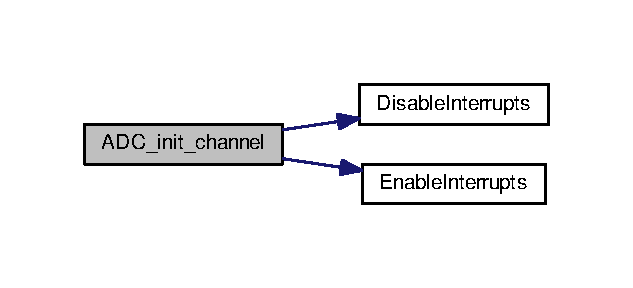
\includegraphics[width=304pt]{_a_d_c_8h_ae7cef9ecd73d25c0931372d21e6be943_cgraph}
\end{center}
\end{figure}




Here is the caller graph for this function\-:
\nopagebreak
\begin{figure}[H]
\begin{center}
\leavevmode
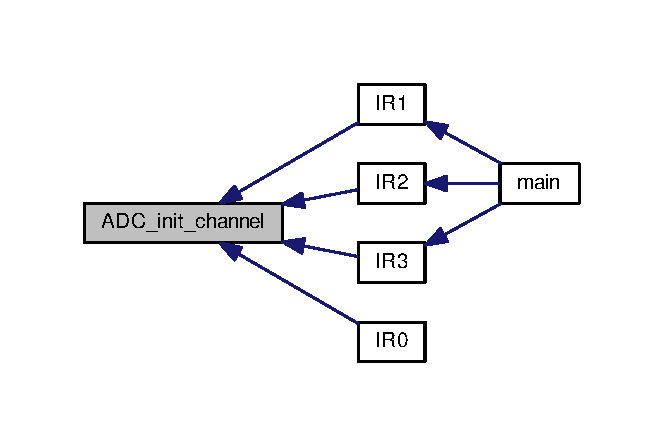
\includegraphics[width=318pt]{_a_d_c_8h_ae7cef9ecd73d25c0931372d21e6be943_icgraph}
\end{center}
\end{figure}


\hypertarget{_a_d_c_8h_a9b319827131872257b8c6a8658852cc0}{\index{A\-D\-C.\-h@{A\-D\-C.\-h}!A\-D\-C\-\_\-\-Open@{A\-D\-C\-\_\-\-Open}}
\index{A\-D\-C\-\_\-\-Open@{A\-D\-C\-\_\-\-Open}!ADC.h@{A\-D\-C.\-h}}
\subsubsection[{A\-D\-C\-\_\-\-Open}]{\setlength{\rightskip}{0pt plus 5cm}int A\-D\-C\-\_\-\-Open (
\begin{DoxyParamCaption}
\item[{unsigned int}]{channel\-Num}
\end{DoxyParamCaption}
)}}\label{_a_d_c_8h_a9b319827131872257b8c6a8658852cc0}


Set up A\-D\-C on specified channel number. 

The parameters are default as follows Timer0\-A\-: enabled Mode\-: 32-\/bit, down counting One-\/shot or periodic\-: periodic Interval value\-: programmable using 32-\/bit period Sample time is bus\-Period$\ast$period sample rate\-: $<$=125,000 samples/second


\begin{DoxyParams}{Parameters}
{\em channel\-Num} & the desired A\-D\-C channel \\
\hline
\end{DoxyParams}
\begin{DoxyReturn}{Returns}
1 if successful, -\/1 for device driver error likely indicating driver already configured. 
\end{DoxyReturn}


Here is the caller graph for this function\-:
\nopagebreak
\begin{figure}[H]
\begin{center}
\leavevmode
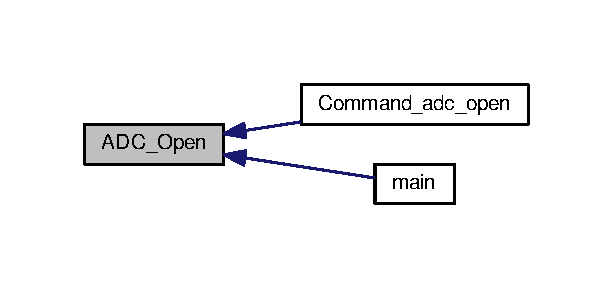
\includegraphics[width=294pt]{_a_d_c_8h_a9b319827131872257b8c6a8658852cc0_icgraph}
\end{center}
\end{figure}


\hypertarget{_a_d_c_8h_a2d0e1be314e7fa00367a329d13e5bbf7}{\index{A\-D\-C.\-h@{A\-D\-C.\-h}!A\-D\-C\-\_\-\-Status@{A\-D\-C\-\_\-\-Status}}
\index{A\-D\-C\-\_\-\-Status@{A\-D\-C\-\_\-\-Status}!ADC.h@{A\-D\-C.\-h}}
\subsubsection[{A\-D\-C\-\_\-\-Status}]{\setlength{\rightskip}{0pt plus 5cm}int A\-D\-C\-\_\-\-Status (
\begin{DoxyParamCaption}
\item[{int}]{id}
\end{DoxyParamCaption}
)}}\label{_a_d_c_8h_a2d0e1be314e7fa00367a329d13e5bbf7}


returns 0 when A\-D\-C\-\_\-collect finishes 

\begin{DoxyReturn}{Returns}
0 if A\-D\-C\-\_\-collect is complete, , else returns the remaining number of samples to record

0 if A\-D\-C\-\_\-collect is complete, else value is the Target\-Count -\/ current Sample\-Count
\end{DoxyReturn}
Acknowledges completion at beginning of handler to minimize sample jitter. since max sample rate is 10\-K\-Hz = 100us at 80\-M\-Hz system clock, I\-S\-R likely to be relatively short. 

Definition at line 237 of file A\-D\-C.\-c.


\begin{DoxyCode}
238 \{
239   \textcolor{keywordflow}{switch}(\textcolor{keywordtype}{id})\{
240     \textcolor{keywordflow}{case} 0: \textcolor{keywordflow}{return} \hyperlink{_a_d_c_8c_a2dda4a471bcd1c89a9e099a5203dd29a}{Collecting}[0]; \textcolor{keywordflow}{break};
241     \textcolor{keywordflow}{case} 1: \textcolor{keywordflow}{return} \hyperlink{_a_d_c_8c_a2dda4a471bcd1c89a9e099a5203dd29a}{Collecting}[1]; \textcolor{keywordflow}{break};
242     \textcolor{keywordflow}{case} 2: \textcolor{keywordflow}{return} \hyperlink{_a_d_c_8c_a2dda4a471bcd1c89a9e099a5203dd29a}{Collecting}[2]; \textcolor{keywordflow}{break};
243     \textcolor{keywordflow}{case} 3: \textcolor{keywordflow}{return} \hyperlink{_a_d_c_8c_a2dda4a471bcd1c89a9e099a5203dd29a}{Collecting}[3]; \textcolor{keywordflow}{break};
244   \}
245 \}
\end{DoxyCode}


Here is the caller graph for this function\-:
\nopagebreak
\begin{figure}[H]
\begin{center}
\leavevmode
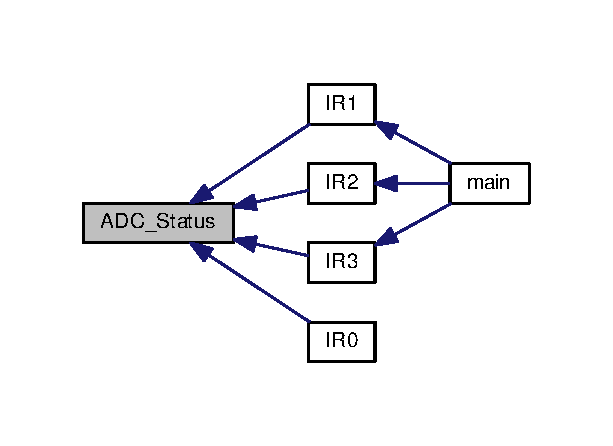
\includegraphics[width=294pt]{_a_d_c_8h_a2d0e1be314e7fa00367a329d13e5bbf7_icgraph}
\end{center}
\end{figure}



\hypertarget{interpreter_8h}{\section{interpreter.\-h File Reference}
\label{interpreter_8h}\index{interpreter.\-h@{interpreter.\-h}}
}
{\ttfamily \#include $<$stdio.\-h$>$}\\*
{\ttfamily \#include $<$string.\-h$>$}\\*
{\ttfamily \#include \char`\"{}S\-T7735.\-h\char`\"{}}\\*
{\ttfamily \#include \char`\"{}A\-D\-C.\-h\char`\"{}}\\*
{\ttfamily \#include \char`\"{}Perf.\-h\char`\"{}}\\*
Include dependency graph for interpreter.\-h\-:
\nopagebreak
\begin{figure}[H]
\begin{center}
\leavevmode
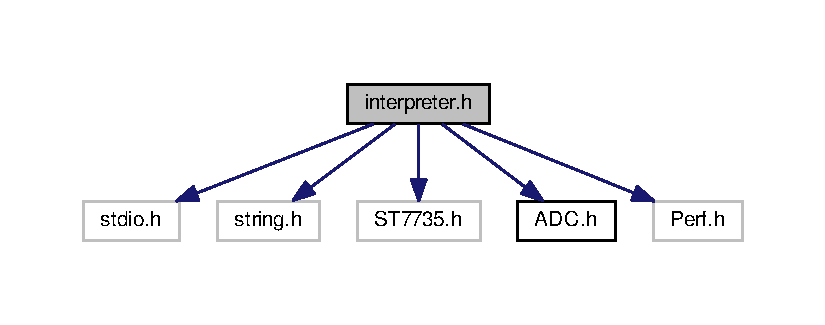
\includegraphics[width=350pt]{interpreter_8h__incl}
\end{center}
\end{figure}
This graph shows which files directly or indirectly include this file\-:
\nopagebreak
\begin{figure}[H]
\begin{center}
\leavevmode
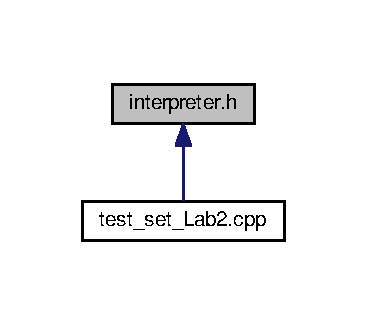
\includegraphics[width=176pt]{interpreter_8h__dep__incl}
\end{center}
\end{figure}
\subsection*{Classes}
\begin{DoxyCompactItemize}
\item 
struct \hyperlink{structcommand}{command}
\end{DoxyCompactItemize}
\subsection*{Macros}
\begin{DoxyCompactItemize}
\item 
\#define \hyperlink{interpreter_8h_a8e475ce8cd5b8c3edf3635605063b571}{C\-O\-M\-M\-A\-N\-D}(N\-A\-M\-E)~\{ \#N\-A\-M\-E, Command\-\_\- \#\# N\-A\-M\-E \}
\item 
\#define \hyperlink{interpreter_8h_a7e897ab5c92350c25d5c49c93c9310f2}{D\-E\-C\-L\-\_\-\-C\-O\-M\-M\-A\-N\-D}(N\-A\-M\-E)~int Command\-\_\- \#\# N\-A\-M\-E \#\# ( char$\ast$ );
\end{DoxyCompactItemize}
\subsection*{Functions}
\begin{DoxyCompactItemize}
\item 
int \hyperlink{interpreter_8h_a10a2c7a55612469a62cd6553e680cdee}{Command\-\_\-disp\-\_\-message} (char $\ast$args)
\item 
int \hyperlink{interpreter_8h_a050e7a28ef711724ac2cba37b6ee4175}{Command\-\_\-list} (char $\ast$args)
\item 
int \hyperlink{interpreter_8h_ab3cd6214932a767bed5e247dedf138d9}{Command\-\_\-adc\-\_\-open} (char $\ast$args)
\item 
int \hyperlink{interpreter_8h_a057b02770d1b0af8a36acf57cbd6de0d}{Command\-\_\-adc\-\_\-in} (char $\ast$args)
\item 
int \hyperlink{interpreter_8h_a2c43f3538cb7b1c0374831eac7961b0d}{Command\-\_\-perf} (char $\ast$args)
\item 
int \hyperlink{interpreter_8h_a09c6bdd753e3c42daa8ef2594db57308}{Command\-\_\-x} (char $\ast$args)
\item 
int \hyperlink{interpreter_8h_a1c46337257556c160f6e6eb9a4259869}{Command\-\_\-y} (char $\ast$args)
\item 
void \hyperlink{interpreter_8h_a08a98a5503e4f3e1a5a19222d425275a}{interpreter} (void)
\end{DoxyCompactItemize}
\subsection*{Variables}
\begin{DoxyCompactItemize}
\item 
struct \hyperlink{structcommand}{command} \hyperlink{interpreter_8h_a18d732036173aa1e51a2e22a6ce78e23}{commands} \mbox{[}$\,$\mbox{]}
\item 
char \hyperlink{interpreter_8h_ab4a03da084e15d3319078d4f4a6bf3ff}{buffer} \mbox{[}64\mbox{]}
\item 
char \hyperlink{interpreter_8h_ad9be07c5c78595ecd8b182a0bde06b1f}{m\-\_\-command} \mbox{[}16\mbox{]}
\end{DoxyCompactItemize}


\subsection{Macro Definition Documentation}
\hypertarget{interpreter_8h_a8e475ce8cd5b8c3edf3635605063b571}{\index{interpreter.\-h@{interpreter.\-h}!C\-O\-M\-M\-A\-N\-D@{C\-O\-M\-M\-A\-N\-D}}
\index{C\-O\-M\-M\-A\-N\-D@{C\-O\-M\-M\-A\-N\-D}!interpreter.h@{interpreter.\-h}}
\subsubsection[{C\-O\-M\-M\-A\-N\-D}]{\setlength{\rightskip}{0pt plus 5cm}\#define C\-O\-M\-M\-A\-N\-D(
\begin{DoxyParamCaption}
\item[{}]{N\-A\-M\-E}
\end{DoxyParamCaption}
)~\{ \#N\-A\-M\-E, Command\-\_\- \#\# N\-A\-M\-E \}}}\label{interpreter_8h_a8e475ce8cd5b8c3edf3635605063b571}


Definition at line 9 of file interpreter.\-h.

\hypertarget{interpreter_8h_a7e897ab5c92350c25d5c49c93c9310f2}{\index{interpreter.\-h@{interpreter.\-h}!D\-E\-C\-L\-\_\-\-C\-O\-M\-M\-A\-N\-D@{D\-E\-C\-L\-\_\-\-C\-O\-M\-M\-A\-N\-D}}
\index{D\-E\-C\-L\-\_\-\-C\-O\-M\-M\-A\-N\-D@{D\-E\-C\-L\-\_\-\-C\-O\-M\-M\-A\-N\-D}!interpreter.h@{interpreter.\-h}}
\subsubsection[{D\-E\-C\-L\-\_\-\-C\-O\-M\-M\-A\-N\-D}]{\setlength{\rightskip}{0pt plus 5cm}\#define D\-E\-C\-L\-\_\-\-C\-O\-M\-M\-A\-N\-D(
\begin{DoxyParamCaption}
\item[{}]{N\-A\-M\-E}
\end{DoxyParamCaption}
)~int Command\-\_\- \#\# N\-A\-M\-E \#\# ( char$\ast$ );}}\label{interpreter_8h_a7e897ab5c92350c25d5c49c93c9310f2}


Definition at line 10 of file interpreter.\-h.



\subsection{Function Documentation}
\hypertarget{interpreter_8h_a057b02770d1b0af8a36acf57cbd6de0d}{\index{interpreter.\-h@{interpreter.\-h}!Command\-\_\-adc\-\_\-in@{Command\-\_\-adc\-\_\-in}}
\index{Command\-\_\-adc\-\_\-in@{Command\-\_\-adc\-\_\-in}!interpreter.h@{interpreter.\-h}}
\subsubsection[{Command\-\_\-adc\-\_\-in}]{\setlength{\rightskip}{0pt plus 5cm}int Command\-\_\-adc\-\_\-in (
\begin{DoxyParamCaption}
\item[{char $\ast$}]{args}
\end{DoxyParamCaption}
)}}\label{interpreter_8h_a057b02770d1b0af8a36acf57cbd6de0d}


Definition at line 116 of file interpreter.\-h.


\begin{DoxyCode}
117 \{
118   \textcolor{keywordtype}{unsigned} \textcolor{keywordtype}{short} result;
119   result = \hyperlink{_a_d_c_8h_a525c5b6cd9976e6405f0bb48cee3ed51}{ADC\_In}();
120   printf(\textcolor{stringliteral}{"ADC value: %f\(\backslash\)n"}, ((\textcolor{keywordtype}{float}) result) *3.3/4096.0);
121   \textcolor{keywordflow}{return} result;
122 \}
\end{DoxyCode}


Here is the call graph for this function\-:
\nopagebreak
\begin{figure}[H]
\begin{center}
\leavevmode
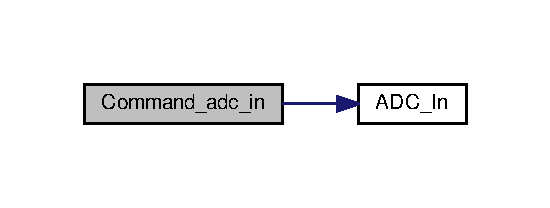
\includegraphics[width=264pt]{interpreter_8h_a057b02770d1b0af8a36acf57cbd6de0d_cgraph}
\end{center}
\end{figure}


\hypertarget{interpreter_8h_ab3cd6214932a767bed5e247dedf138d9}{\index{interpreter.\-h@{interpreter.\-h}!Command\-\_\-adc\-\_\-open@{Command\-\_\-adc\-\_\-open}}
\index{Command\-\_\-adc\-\_\-open@{Command\-\_\-adc\-\_\-open}!interpreter.h@{interpreter.\-h}}
\subsubsection[{Command\-\_\-adc\-\_\-open}]{\setlength{\rightskip}{0pt plus 5cm}int Command\-\_\-adc\-\_\-open (
\begin{DoxyParamCaption}
\item[{char $\ast$}]{args}
\end{DoxyParamCaption}
)}}\label{interpreter_8h_ab3cd6214932a767bed5e247dedf138d9}


Definition at line 109 of file interpreter.\-h.


\begin{DoxyCode}
110 \{
111   \textcolor{keywordtype}{unsigned} \textcolor{keywordtype}{int} channel;
112   sscanf(args, \textcolor{stringliteral}{"%u"}, &channel);
113   \textcolor{keywordflow}{return} \hyperlink{_a_d_c_8h_a9b319827131872257b8c6a8658852cc0}{ADC\_Open}(channel);
114 \}
\end{DoxyCode}


Here is the call graph for this function\-:
\nopagebreak
\begin{figure}[H]
\begin{center}
\leavevmode
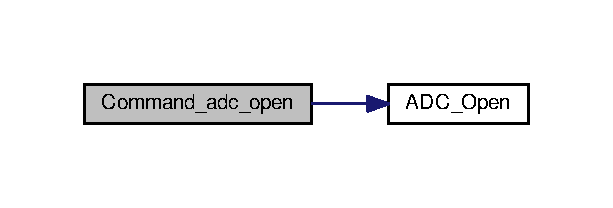
\includegraphics[width=294pt]{interpreter_8h_ab3cd6214932a767bed5e247dedf138d9_cgraph}
\end{center}
\end{figure}


\hypertarget{interpreter_8h_a10a2c7a55612469a62cd6553e680cdee}{\index{interpreter.\-h@{interpreter.\-h}!Command\-\_\-disp\-\_\-message@{Command\-\_\-disp\-\_\-message}}
\index{Command\-\_\-disp\-\_\-message@{Command\-\_\-disp\-\_\-message}!interpreter.h@{interpreter.\-h}}
\subsubsection[{Command\-\_\-disp\-\_\-message}]{\setlength{\rightskip}{0pt plus 5cm}int Command\-\_\-disp\-\_\-message (
\begin{DoxyParamCaption}
\item[{char $\ast$}]{args}
\end{DoxyParamCaption}
)}}\label{interpreter_8h_a10a2c7a55612469a62cd6553e680cdee}


Definition at line 96 of file interpreter.\-h.


\begin{DoxyCode}
97 \{
98   \textcolor{comment}{//printf("Not implemented yet\(\backslash\)n");}
99   \textcolor{keywordtype}{int} disp, line;\textcolor{comment}{//, n;}
100   \textcolor{keywordtype}{char} str[64];
101   sscanf(args, \textcolor{stringliteral}{"%d %d %[^\(\backslash\)t\(\backslash\)r\(\backslash\)n]"}, &disp, &line, str);
102   \textcolor{comment}{//str = args + n;}
103   printf(\textcolor{stringliteral}{"\(\backslash\)n Got disp=%d\(\backslash\)tline=%d, %s\(\backslash\)n"}, disp, line, str);
104 \textcolor{comment}{//  ST7735\_Message(disp, line, str, 0);    }
105 
106   \textcolor{keywordflow}{return} -1;
107 \}
\end{DoxyCode}
\hypertarget{interpreter_8h_a050e7a28ef711724ac2cba37b6ee4175}{\index{interpreter.\-h@{interpreter.\-h}!Command\-\_\-list@{Command\-\_\-list}}
\index{Command\-\_\-list@{Command\-\_\-list}!interpreter.h@{interpreter.\-h}}
\subsubsection[{Command\-\_\-list}]{\setlength{\rightskip}{0pt plus 5cm}int Command\-\_\-list (
\begin{DoxyParamCaption}
\item[{char $\ast$}]{args}
\end{DoxyParamCaption}
)}}\label{interpreter_8h_a050e7a28ef711724ac2cba37b6ee4175}


Definition at line 84 of file interpreter.\-h.


\begin{DoxyCode}
85 \{
86   \textcolor{keyword}{struct }\hyperlink{structcommand}{command}* command\_ptr = \hyperlink{interpreter_8h_a18d732036173aa1e51a2e22a6ce78e23}{commands};
87   \textcolor{keyword}{struct }\hyperlink{structcommand}{command}* end\_ptr = command\_ptr + \textcolor{keyword}{sizeof}(\hyperlink{interpreter_8h_a18d732036173aa1e51a2e22a6ce78e23}{commands})/\textcolor{keyword}{sizeof}(
      \hyperlink{interpreter_8h_a18d732036173aa1e51a2e22a6ce78e23}{commands}[0]);
88 
89   \textcolor{keywordflow}{while}(command\_ptr < end\_ptr)\{
90     printf(\textcolor{stringliteral}{"%s\(\backslash\)n"}, command\_ptr->\hyperlink{structcommand_a556cd9d8b435c0017704254f3d9a3e57}{label});
91     command\_ptr++;
92   \}
93   \textcolor{keywordflow}{return} 0;
94 \}
\end{DoxyCode}
\hypertarget{interpreter_8h_a2c43f3538cb7b1c0374831eac7961b0d}{\index{interpreter.\-h@{interpreter.\-h}!Command\-\_\-perf@{Command\-\_\-perf}}
\index{Command\-\_\-perf@{Command\-\_\-perf}!interpreter.h@{interpreter.\-h}}
\subsubsection[{Command\-\_\-perf}]{\setlength{\rightskip}{0pt plus 5cm}int Command\-\_\-perf (
\begin{DoxyParamCaption}
\item[{char $\ast$}]{args}
\end{DoxyParamCaption}
)}}\label{interpreter_8h_a2c43f3538cb7b1c0374831eac7961b0d}


Definition at line 125 of file interpreter.\-h.


\begin{DoxyCode}
125                             \{
126   printf(\textcolor{stringliteral}{"\(\backslash\)nJitter: %d\(\backslash\)nNumSamples: %d\(\backslash\)nNumCreated: %d\(\backslash\)nDataLost: %d\(\backslash\)n"}, jitter, NumSamples, NumCreated, 
      DataLost  );
127   \textcolor{keywordflow}{return} 1;
128 \}
\end{DoxyCode}
\hypertarget{interpreter_8h_a09c6bdd753e3c42daa8ef2594db57308}{\index{interpreter.\-h@{interpreter.\-h}!Command\-\_\-x@{Command\-\_\-x}}
\index{Command\-\_\-x@{Command\-\_\-x}!interpreter.h@{interpreter.\-h}}
\subsubsection[{Command\-\_\-x}]{\setlength{\rightskip}{0pt plus 5cm}int Command\-\_\-x (
\begin{DoxyParamCaption}
\item[{char $\ast$}]{args}
\end{DoxyParamCaption}
)}}\label{interpreter_8h_a09c6bdd753e3c42daa8ef2594db57308}


Definition at line 129 of file interpreter.\-h.


\begin{DoxyCode}
129                          \{
130   \textcolor{keywordtype}{int} i;
131   \textcolor{keywordflow}{for}(i = 0; i < 64; i++)\{
132     printf(\textcolor{stringliteral}{"\(\backslash\)n"});
133     printf(\textcolor{stringliteral}{"%ld\(\backslash\)t"}, (3000*x[i])/4096);
134   \}
135   \textcolor{keywordflow}{return} 1;
136 \}
\end{DoxyCode}
\hypertarget{interpreter_8h_a1c46337257556c160f6e6eb9a4259869}{\index{interpreter.\-h@{interpreter.\-h}!Command\-\_\-y@{Command\-\_\-y}}
\index{Command\-\_\-y@{Command\-\_\-y}!interpreter.h@{interpreter.\-h}}
\subsubsection[{Command\-\_\-y}]{\setlength{\rightskip}{0pt plus 5cm}int Command\-\_\-y (
\begin{DoxyParamCaption}
\item[{char $\ast$}]{args}
\end{DoxyParamCaption}
)}}\label{interpreter_8h_a1c46337257556c160f6e6eb9a4259869}


Definition at line 137 of file interpreter.\-h.


\begin{DoxyCode}
137                          \{
138   \textcolor{keywordtype}{int} i;
139   \textcolor{keywordflow}{for}( i = 0; i < 64; i++)\{
140     printf(\textcolor{stringliteral}{"\(\backslash\)n"});
141     printf(\textcolor{stringliteral}{"%ld\(\backslash\)t"}, y[i]);
142   \}
143   \textcolor{keywordflow}{return} 1;
144 \}
\end{DoxyCode}
\hypertarget{interpreter_8h_a08a98a5503e4f3e1a5a19222d425275a}{\index{interpreter.\-h@{interpreter.\-h}!interpreter@{interpreter}}
\index{interpreter@{interpreter}!interpreter.h@{interpreter.\-h}}
\subsubsection[{interpreter}]{\setlength{\rightskip}{0pt plus 5cm}void interpreter (
\begin{DoxyParamCaption}
\item[{void}]{}
\end{DoxyParamCaption}
)}}\label{interpreter_8h_a08a98a5503e4f3e1a5a19222d425275a}


Definition at line 53 of file interpreter.\-h.


\begin{DoxyCode}
53                       \{
54   \textcolor{keywordtype}{char} *buff\_ptr = \hyperlink{interpreter_8h_ab4a03da084e15d3319078d4f4a6bf3ff}{buffer};
55   \textcolor{keyword}{struct }\hyperlink{structcommand}{command}* command\_ptr = \hyperlink{interpreter_8h_a18d732036173aa1e51a2e22a6ce78e23}{commands};
56   \textcolor{keyword}{struct }\hyperlink{structcommand}{command}* end\_ptr = command\_ptr + \textcolor{keyword}{sizeof}(\hyperlink{interpreter_8h_a18d732036173aa1e51a2e22a6ce78e23}{commands})/\textcolor{keyword}{sizeof}(
      \hyperlink{interpreter_8h_a18d732036173aa1e51a2e22a6ce78e23}{commands}[0]);
57   int (*\textcolor{keyword}{function})(\textcolor{keywordtype}{char} *);
58   \textcolor{keywordtype}{int} n;
59   printf(\textcolor{stringliteral}{">> "});
60   \textcolor{comment}{//scanf("%s\(\backslash\)n", buffer); //, buffer);}
61   fgets(\hyperlink{interpreter_8h_ab4a03da084e15d3319078d4f4a6bf3ff}{buffer}, 64, stdin);
62   sscanf(buff\_ptr, \textcolor{stringliteral}{"%s%n"}, \hyperlink{interpreter_8h_ad9be07c5c78595ecd8b182a0bde06b1f}{m\_command}, &n);
63   printf(\textcolor{stringliteral}{"m\_command: %s\(\backslash\)n"}, \hyperlink{interpreter_8h_ad9be07c5c78595ecd8b182a0bde06b1f}{m\_command});
64     buff\_ptr += n;
65   printf(\textcolor{stringliteral}{"%s\(\backslash\)n"}, buff\_ptr);
66     \textcolor{comment}{//printf("Buffer: %s\(\backslash\)n", buff\_ptr);}
67   \textcolor{keywordflow}{while} (command\_ptr < end\_ptr)\{
68     \textcolor{keyword}{function} = command\_ptr->\hyperlink{structcommand_a217dfc1d06446ee6606a9a007fa6a7b6}{function};
69     \textcolor{keywordflow}{if}(strcmp(\hyperlink{interpreter_8h_ad9be07c5c78595ecd8b182a0bde06b1f}{m\_command}, command\_ptr->\hyperlink{structcommand_a556cd9d8b435c0017704254f3d9a3e57}{label}) == 0)\{
70 \textcolor{comment}{//      printf("Doing Command: %s\(\backslash\)n", command\_ptr->label);}
71       \textcolor{keyword}{function}(buff\_ptr);
72       
73       \textcolor{keywordflow}{return};
74     \}
75 
76     command\_ptr++;
77   \}
78   printf(\textcolor{stringliteral}{"[Warning] Interpreter Command not found\(\backslash\)n"});
79   \textcolor{keywordflow}{return};
80 \}
\end{DoxyCode}


Here is the caller graph for this function\-:
\nopagebreak
\begin{figure}[H]
\begin{center}
\leavevmode
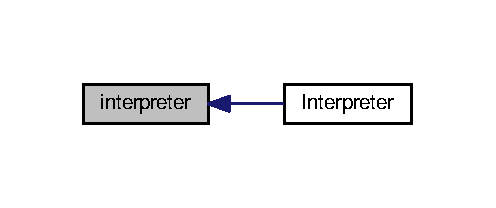
\includegraphics[width=238pt]{interpreter_8h_a08a98a5503e4f3e1a5a19222d425275a_icgraph}
\end{center}
\end{figure}




\subsection{Variable Documentation}
\hypertarget{interpreter_8h_ab4a03da084e15d3319078d4f4a6bf3ff}{\index{interpreter.\-h@{interpreter.\-h}!buffer@{buffer}}
\index{buffer@{buffer}!interpreter.h@{interpreter.\-h}}
\subsubsection[{buffer}]{\setlength{\rightskip}{0pt plus 5cm}char buffer\mbox{[}64\mbox{]}}}\label{interpreter_8h_ab4a03da084e15d3319078d4f4a6bf3ff}


Definition at line 51 of file interpreter.\-h.

\hypertarget{interpreter_8h_a18d732036173aa1e51a2e22a6ce78e23}{\index{interpreter.\-h@{interpreter.\-h}!commands@{commands}}
\index{commands@{commands}!interpreter.h@{interpreter.\-h}}
\subsubsection[{commands}]{\setlength{\rightskip}{0pt plus 5cm}struct {\bf command} commands\mbox{[}$\,$\mbox{]}}}\label{interpreter_8h_a18d732036173aa1e51a2e22a6ce78e23}
{\bfseries Initial value\-:}
\begin{DoxyCode}
=
\{
  \{ \textcolor{stringliteral}{"list"}, \hyperlink{interpreter_8h_a050e7a28ef711724ac2cba37b6ee4175}{Command\_list}  \},
  \{ \textcolor{stringliteral}{"disp\_message"}, \hyperlink{interpreter_8h_a10a2c7a55612469a62cd6553e680cdee}{Command\_disp\_message}  \},
  \{ \textcolor{stringliteral}{"adc\_open"}, \hyperlink{interpreter_8h_ab3cd6214932a767bed5e247dedf138d9}{Command\_adc\_open}  \},
  \{ \textcolor{stringliteral}{"adc\_in"}, \hyperlink{interpreter_8h_a057b02770d1b0af8a36acf57cbd6de0d}{Command\_adc\_in}  \},       
  \{ \textcolor{stringliteral}{"perf"}, \hyperlink{interpreter_8h_a2c43f3538cb7b1c0374831eac7961b0d}{Command\_perf}  \},
  \{ \textcolor{stringliteral}{"x"}, \hyperlink{interpreter_8h_a09c6bdd753e3c42daa8ef2594db57308}{Command\_x}  \},
  \{ \textcolor{stringliteral}{"y"}, \hyperlink{interpreter_8h_a1c46337257556c160f6e6eb9a4259869}{Command\_y}  \}
  

\}
\end{DoxyCode}


Definition at line 32 of file interpreter.\-h.

\hypertarget{interpreter_8h_ad9be07c5c78595ecd8b182a0bde06b1f}{\index{interpreter.\-h@{interpreter.\-h}!m\-\_\-command@{m\-\_\-command}}
\index{m\-\_\-command@{m\-\_\-command}!interpreter.h@{interpreter.\-h}}
\subsubsection[{m\-\_\-command}]{\setlength{\rightskip}{0pt plus 5cm}char m\-\_\-command\mbox{[}16\mbox{]}}}\label{interpreter_8h_ad9be07c5c78595ecd8b182a0bde06b1f}


Definition at line 52 of file interpreter.\-h.


\hypertarget{_lab5_8c}{\section{Lab5.\-c File Reference}
\label{_lab5_8c}\index{Lab5.\-c@{Lab5.\-c}}
}
{\ttfamily \#include $<$stdio.\-h$>$}\\*
{\ttfamily \#include $<$string.\-h$>$}\\*
{\ttfamily \#include \char`\"{}inc/hw\-\_\-types.\-h\char`\"{}}\\*
{\ttfamily \#include \char`\"{}A\-D\-C.\-h\char`\"{}}\\*
{\ttfamily \#include \char`\"{}os.\-h\char`\"{}}\\*
{\ttfamily \#include \char`\"{}inc/tm4c123gh6pm.\-h\char`\"{}}\\*
{\ttfamily \#include \char`\"{}edisk.\-h\char`\"{}}\\*
{\ttfamily \#include \char`\"{}efile.\-h\char`\"{}}\\*
{\ttfamily \#include \char`\"{}Perf.\-h\char`\"{}}\\*
Include dependency graph for Lab5.\-c\-:
\nopagebreak
\begin{figure}[H]
\begin{center}
\leavevmode
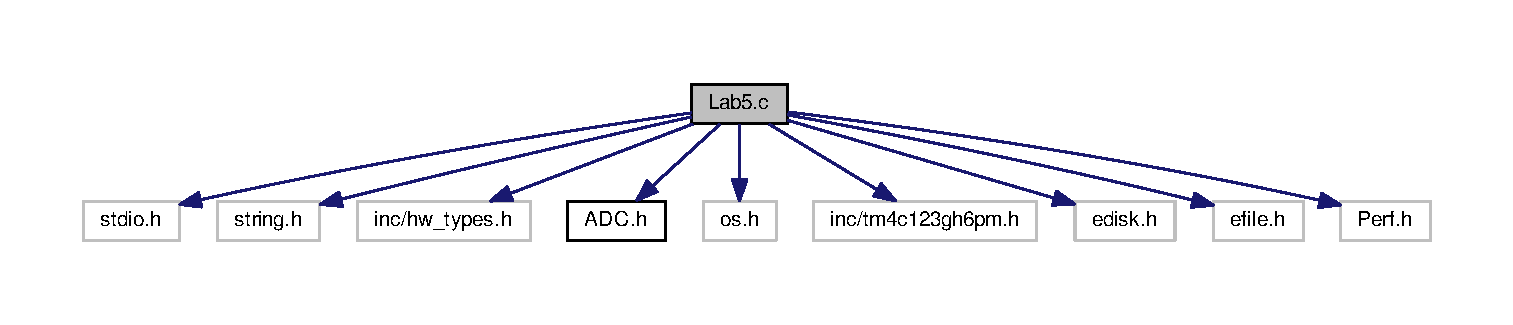
\includegraphics[width=350pt]{_lab5_8c__incl}
\end{center}
\end{figure}
\subsection*{Macros}
\begin{DoxyCompactItemize}
\item 
\#define \hyperlink{_lab5_8c_ae586204918bfbea259810829a239d886}{T\-I\-M\-E\-S\-L\-I\-C\-E}~2$\ast$T\-I\-M\-E\-\_\-1\-M\-S
\item 
\#define \hyperlink{_lab5_8c_ab527c0e4b7c318dbae300412b03eed17}{G\-P\-I\-O\-\_\-\-P\-F0}~($\ast$((volatile unsigned long $\ast$)0x40025004))
\item 
\#define \hyperlink{_lab5_8c_abbb42535d15ee2366af5a5b1e2124a05}{G\-P\-I\-O\-\_\-\-P\-F1}~($\ast$((volatile unsigned long $\ast$)0x40025008))
\item 
\#define \hyperlink{_lab5_8c_a959a99608831fef309047e405b5059bc}{G\-P\-I\-O\-\_\-\-P\-F2}~($\ast$((volatile unsigned long $\ast$)0x40025010))
\item 
\#define \hyperlink{_lab5_8c_aab864bd67f4cea10fd17ee13808668cd}{G\-P\-I\-O\-\_\-\-P\-F3}~($\ast$((volatile unsigned long $\ast$)0x40025020))
\item 
\#define \hyperlink{_lab5_8c_a66dc5c770ec2c27da7ecceb303354ff4}{G\-P\-I\-O\-\_\-\-P\-G1}~($\ast$((volatile unsigned long $\ast$)0x40026008))
\item 
\#define \hyperlink{_lab5_8c_ab9438454509c495abb6f0dac60d7ac02}{P\-E0}~($\ast$((volatile unsigned long $\ast$)0x40024004))
\item 
\#define \hyperlink{_lab5_8c_a2b333e81f2f724f5d0f6ff557f3a0b49}{P\-E1}~($\ast$((volatile unsigned long $\ast$)0x40024008))
\item 
\#define \hyperlink{_lab5_8c_ab9f47403c8a3489beafcac840b8fff7d}{P\-E2}~($\ast$((volatile unsigned long $\ast$)0x40024010))
\item 
\#define \hyperlink{_lab5_8c_a1ef39ee2274d28bab6daa26359630c57}{P\-E3}~($\ast$((volatile unsigned long $\ast$)0x40024020))
\item 
\#define \hyperlink{_lab5_8c_a02723c1cf9784c591e45af7bf584f97c}{M\-A\-X\-B\-L\-O\-C\-K\-S}~100
\end{DoxyCompactItemize}
\subsection*{Functions}
\begin{DoxyCompactItemize}
\item 
void \hyperlink{_lab5_8c_a5b51a90348618cbd5eb0e65114ea0daf}{Port\-E\-\_\-\-Init} (void)
\item 
void \hyperlink{_lab5_8c_aefdc786873bfd8245aa0f47e54f3077e}{Robot} (void)
\item 
void \hyperlink{_lab5_8c_af31c52c818cfe90014abf63e1b984ca0}{Button\-Push} (void)
\item 
void \hyperlink{_lab5_8c_a6141d7655f515388f7e5323b9e0a81b3}{Down\-Push} (void)
\item 
void \hyperlink{_lab5_8c_a7eaf80f6bdd1fd573219220dbb7f8837}{Producer} (unsigned long data)
\item 
void \hyperlink{_lab5_8c_a269a2b542c489c0d00dd5d4328ed6ccf}{Idle\-Task} (void)
\item 
void \hyperlink{_lab5_8c_a2e36aaea6b9cab2ca1faab2c2d760271}{Interpreter} (void)
\item 
int \hyperlink{_lab5_8c_a7eff0fb752de46f3df0342f22f69c458}{realmain} (void)
\item 
void \hyperlink{_lab5_8c_a22c9a06aa7985e858ece98451d29d482}{disk\-Error} (char $\ast$errtype, unsigned long n)
\item 
void \hyperlink{_lab5_8c_a3efcf5e79ed9738d40e3dbaf3befc678}{Test\-Disk} (void)
\item 
void \hyperlink{_lab5_8c_a8ae9923a4397b1cc33baf08ea2341c33}{Run\-Test} (void)
\item 
void \hyperlink{_lab5_8c_a95d7d847e2c29bc8c83224318399d41b}{Test\-File} (void)
\item 
int \hyperlink{_lab5_8c_abbcfdc8ab315a9f273a0c498a0e73e29}{testmain2} (void)
\item 
void \hyperlink{_lab5_8c_aad6d0bf2cbb02582664e1107ccee3483}{Test\-F\-A\-T} (void)
\item 
uint32\-\_\-t \hyperlink{_lab5_8c_a9c8a4d21a75e6a19ea31df0c5ccecfc2}{Ping} (void)
\item 
void \hyperlink{_lab5_8c_ad4c2bdb78f3b09301fc0a24bbc9d1a5d}{Test\-Us} (void)
\item 
int \hyperlink{_lab5_8c_a840291bc02cba5474a4cb46a9b9566fe}{main} (void)
\end{DoxyCompactItemize}
\subsection*{Variables}
\begin{DoxyCompactItemize}
\item 
int \hyperlink{_lab5_8c_a1e26c569f8ea4c8145952219697f181f}{Running}
\item 
unsigned long \hyperlink{_lab5_8c_a1bb5d517b380a841c91444d3bbffb9ab}{Idlecount} =0
\item 
unsigned char \hyperlink{_lab5_8c_a9516ea594e030f96eb9483d95f1583a5}{buffer} \mbox{[}512\mbox{]}
\end{DoxyCompactItemize}


\subsection{Macro Definition Documentation}
\hypertarget{_lab5_8c_ab527c0e4b7c318dbae300412b03eed17}{\index{Lab5.\-c@{Lab5.\-c}!G\-P\-I\-O\-\_\-\-P\-F0@{G\-P\-I\-O\-\_\-\-P\-F0}}
\index{G\-P\-I\-O\-\_\-\-P\-F0@{G\-P\-I\-O\-\_\-\-P\-F0}!Lab5.c@{Lab5.\-c}}
\subsubsection[{G\-P\-I\-O\-\_\-\-P\-F0}]{\setlength{\rightskip}{0pt plus 5cm}\#define G\-P\-I\-O\-\_\-\-P\-F0~($\ast$((volatile unsigned long $\ast$)0x40025004))}}\label{_lab5_8c_ab527c0e4b7c318dbae300412b03eed17}


Definition at line 27 of file Lab5.\-c.

\hypertarget{_lab5_8c_abbb42535d15ee2366af5a5b1e2124a05}{\index{Lab5.\-c@{Lab5.\-c}!G\-P\-I\-O\-\_\-\-P\-F1@{G\-P\-I\-O\-\_\-\-P\-F1}}
\index{G\-P\-I\-O\-\_\-\-P\-F1@{G\-P\-I\-O\-\_\-\-P\-F1}!Lab5.c@{Lab5.\-c}}
\subsubsection[{G\-P\-I\-O\-\_\-\-P\-F1}]{\setlength{\rightskip}{0pt plus 5cm}\#define G\-P\-I\-O\-\_\-\-P\-F1~($\ast$((volatile unsigned long $\ast$)0x40025008))}}\label{_lab5_8c_abbb42535d15ee2366af5a5b1e2124a05}


Definition at line 28 of file Lab5.\-c.

\hypertarget{_lab5_8c_a959a99608831fef309047e405b5059bc}{\index{Lab5.\-c@{Lab5.\-c}!G\-P\-I\-O\-\_\-\-P\-F2@{G\-P\-I\-O\-\_\-\-P\-F2}}
\index{G\-P\-I\-O\-\_\-\-P\-F2@{G\-P\-I\-O\-\_\-\-P\-F2}!Lab5.c@{Lab5.\-c}}
\subsubsection[{G\-P\-I\-O\-\_\-\-P\-F2}]{\setlength{\rightskip}{0pt plus 5cm}\#define G\-P\-I\-O\-\_\-\-P\-F2~($\ast$((volatile unsigned long $\ast$)0x40025010))}}\label{_lab5_8c_a959a99608831fef309047e405b5059bc}


Definition at line 29 of file Lab5.\-c.

\hypertarget{_lab5_8c_aab864bd67f4cea10fd17ee13808668cd}{\index{Lab5.\-c@{Lab5.\-c}!G\-P\-I\-O\-\_\-\-P\-F3@{G\-P\-I\-O\-\_\-\-P\-F3}}
\index{G\-P\-I\-O\-\_\-\-P\-F3@{G\-P\-I\-O\-\_\-\-P\-F3}!Lab5.c@{Lab5.\-c}}
\subsubsection[{G\-P\-I\-O\-\_\-\-P\-F3}]{\setlength{\rightskip}{0pt plus 5cm}\#define G\-P\-I\-O\-\_\-\-P\-F3~($\ast$((volatile unsigned long $\ast$)0x40025020))}}\label{_lab5_8c_aab864bd67f4cea10fd17ee13808668cd}


Definition at line 30 of file Lab5.\-c.

\hypertarget{_lab5_8c_a66dc5c770ec2c27da7ecceb303354ff4}{\index{Lab5.\-c@{Lab5.\-c}!G\-P\-I\-O\-\_\-\-P\-G1@{G\-P\-I\-O\-\_\-\-P\-G1}}
\index{G\-P\-I\-O\-\_\-\-P\-G1@{G\-P\-I\-O\-\_\-\-P\-G1}!Lab5.c@{Lab5.\-c}}
\subsubsection[{G\-P\-I\-O\-\_\-\-P\-G1}]{\setlength{\rightskip}{0pt plus 5cm}\#define G\-P\-I\-O\-\_\-\-P\-G1~($\ast$((volatile unsigned long $\ast$)0x40026008))}}\label{_lab5_8c_a66dc5c770ec2c27da7ecceb303354ff4}


Definition at line 31 of file Lab5.\-c.

\hypertarget{_lab5_8c_a02723c1cf9784c591e45af7bf584f97c}{\index{Lab5.\-c@{Lab5.\-c}!M\-A\-X\-B\-L\-O\-C\-K\-S@{M\-A\-X\-B\-L\-O\-C\-K\-S}}
\index{M\-A\-X\-B\-L\-O\-C\-K\-S@{M\-A\-X\-B\-L\-O\-C\-K\-S}!Lab5.c@{Lab5.\-c}}
\subsubsection[{M\-A\-X\-B\-L\-O\-C\-K\-S}]{\setlength{\rightskip}{0pt plus 5cm}\#define M\-A\-X\-B\-L\-O\-C\-K\-S~100}}\label{_lab5_8c_a02723c1cf9784c591e45af7bf584f97c}


Definition at line 183 of file Lab5.\-c.

\hypertarget{_lab5_8c_ab9438454509c495abb6f0dac60d7ac02}{\index{Lab5.\-c@{Lab5.\-c}!P\-E0@{P\-E0}}
\index{P\-E0@{P\-E0}!Lab5.c@{Lab5.\-c}}
\subsubsection[{P\-E0}]{\setlength{\rightskip}{0pt plus 5cm}\#define P\-E0~($\ast$((volatile unsigned long $\ast$)0x40024004))}}\label{_lab5_8c_ab9438454509c495abb6f0dac60d7ac02}


Definition at line 33 of file Lab5.\-c.

\hypertarget{_lab5_8c_a2b333e81f2f724f5d0f6ff557f3a0b49}{\index{Lab5.\-c@{Lab5.\-c}!P\-E1@{P\-E1}}
\index{P\-E1@{P\-E1}!Lab5.c@{Lab5.\-c}}
\subsubsection[{P\-E1}]{\setlength{\rightskip}{0pt plus 5cm}\#define P\-E1~($\ast$((volatile unsigned long $\ast$)0x40024008))}}\label{_lab5_8c_a2b333e81f2f724f5d0f6ff557f3a0b49}


Definition at line 34 of file Lab5.\-c.

\hypertarget{_lab5_8c_ab9f47403c8a3489beafcac840b8fff7d}{\index{Lab5.\-c@{Lab5.\-c}!P\-E2@{P\-E2}}
\index{P\-E2@{P\-E2}!Lab5.c@{Lab5.\-c}}
\subsubsection[{P\-E2}]{\setlength{\rightskip}{0pt plus 5cm}\#define P\-E2~($\ast$((volatile unsigned long $\ast$)0x40024010))}}\label{_lab5_8c_ab9f47403c8a3489beafcac840b8fff7d}


Definition at line 35 of file Lab5.\-c.

\hypertarget{_lab5_8c_a1ef39ee2274d28bab6daa26359630c57}{\index{Lab5.\-c@{Lab5.\-c}!P\-E3@{P\-E3}}
\index{P\-E3@{P\-E3}!Lab5.c@{Lab5.\-c}}
\subsubsection[{P\-E3}]{\setlength{\rightskip}{0pt plus 5cm}\#define P\-E3~($\ast$((volatile unsigned long $\ast$)0x40024020))}}\label{_lab5_8c_a1ef39ee2274d28bab6daa26359630c57}


Definition at line 36 of file Lab5.\-c.

\hypertarget{_lab5_8c_ae586204918bfbea259810829a239d886}{\index{Lab5.\-c@{Lab5.\-c}!T\-I\-M\-E\-S\-L\-I\-C\-E@{T\-I\-M\-E\-S\-L\-I\-C\-E}}
\index{T\-I\-M\-E\-S\-L\-I\-C\-E@{T\-I\-M\-E\-S\-L\-I\-C\-E}!Lab5.c@{Lab5.\-c}}
\subsubsection[{T\-I\-M\-E\-S\-L\-I\-C\-E}]{\setlength{\rightskip}{0pt plus 5cm}\#define T\-I\-M\-E\-S\-L\-I\-C\-E~2$\ast$T\-I\-M\-E\-\_\-1\-M\-S}}\label{_lab5_8c_ae586204918bfbea259810829a239d886}


Definition at line 25 of file Lab5.\-c.



\subsection{Function Documentation}
\hypertarget{_lab5_8c_af31c52c818cfe90014abf63e1b984ca0}{\index{Lab5.\-c@{Lab5.\-c}!Button\-Push@{Button\-Push}}
\index{Button\-Push@{Button\-Push}!Lab5.c@{Lab5.\-c}}
\subsubsection[{Button\-Push}]{\setlength{\rightskip}{0pt plus 5cm}void Button\-Push (
\begin{DoxyParamCaption}
\item[{void}]{}
\end{DoxyParamCaption}
)}}\label{_lab5_8c_af31c52c818cfe90014abf63e1b984ca0}


Definition at line 89 of file Lab5.\-c.


\begin{DoxyCode}
89                      \{
90   \textcolor{keywordflow}{if}(\hyperlink{_lab5_8c_a1e26c569f8ea4c8145952219697f181f}{Running}==0)\{
91     \hyperlink{_lab5_8c_a1e26c569f8ea4c8145952219697f181f}{Running} = 1;  \textcolor{comment}{// prevents you from starting two robot threads}
92     NumCreated += OS\_AddThread(&\hyperlink{_lab5_8c_aefdc786873bfd8245aa0f47e54f3077e}{Robot},128,1);  \textcolor{comment}{// start a 20 second run}
93   \}
94 \}
\end{DoxyCode}


Here is the call graph for this function\-:
\nopagebreak
\begin{figure}[H]
\begin{center}
\leavevmode
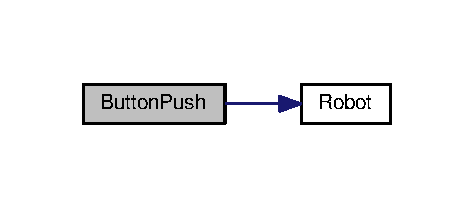
\includegraphics[width=228pt]{_lab5_8c_af31c52c818cfe90014abf63e1b984ca0_cgraph}
\end{center}
\end{figure}


\hypertarget{_lab5_8c_a22c9a06aa7985e858ece98451d29d482}{\index{Lab5.\-c@{Lab5.\-c}!disk\-Error@{disk\-Error}}
\index{disk\-Error@{disk\-Error}!Lab5.c@{Lab5.\-c}}
\subsubsection[{disk\-Error}]{\setlength{\rightskip}{0pt plus 5cm}void disk\-Error (
\begin{DoxyParamCaption}
\item[{char $\ast$}]{errtype, }
\item[{unsigned long}]{n}
\end{DoxyParamCaption}
)}}\label{_lab5_8c_a22c9a06aa7985e858ece98451d29d482}


Definition at line 184 of file Lab5.\-c.


\begin{DoxyCode}
184                                               \{
185   printf(errtype);
186   printf(\textcolor{stringliteral}{" disk error %u"},n);
187   OS\_Kill();
188 \}
\end{DoxyCode}


Here is the caller graph for this function\-:
\nopagebreak
\begin{figure}[H]
\begin{center}
\leavevmode
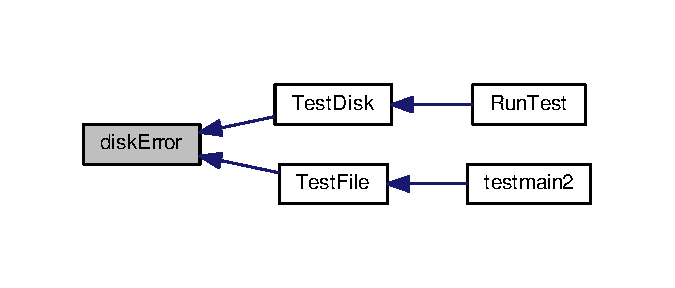
\includegraphics[width=324pt]{_lab5_8c_a22c9a06aa7985e858ece98451d29d482_icgraph}
\end{center}
\end{figure}


\hypertarget{_lab5_8c_a6141d7655f515388f7e5323b9e0a81b3}{\index{Lab5.\-c@{Lab5.\-c}!Down\-Push@{Down\-Push}}
\index{Down\-Push@{Down\-Push}!Lab5.c@{Lab5.\-c}}
\subsubsection[{Down\-Push}]{\setlength{\rightskip}{0pt plus 5cm}void Down\-Push (
\begin{DoxyParamCaption}
\item[{void}]{}
\end{DoxyParamCaption}
)}}\label{_lab5_8c_a6141d7655f515388f7e5323b9e0a81b3}


Definition at line 98 of file Lab5.\-c.


\begin{DoxyCode}
98                    \{
99 
100 \}
\end{DoxyCode}
\hypertarget{_lab5_8c_a269a2b542c489c0d00dd5d4328ed6ccf}{\index{Lab5.\-c@{Lab5.\-c}!Idle\-Task@{Idle\-Task}}
\index{Idle\-Task@{Idle\-Task}!Lab5.c@{Lab5.\-c}}
\subsubsection[{Idle\-Task}]{\setlength{\rightskip}{0pt plus 5cm}void Idle\-Task (
\begin{DoxyParamCaption}
\item[{void}]{}
\end{DoxyParamCaption}
)}}\label{_lab5_8c_a269a2b542c489c0d00dd5d4328ed6ccf}


Definition at line 129 of file Lab5.\-c.


\begin{DoxyCode}
129                    \{ 
130   \textcolor{keywordflow}{while}(1) \{ 
131     \hyperlink{_lab5_8c_a1bb5d517b380a841c91444d3bbffb9ab}{Idlecount}++;        \textcolor{comment}{// debugging }
132   \}
133 \}
\end{DoxyCode}


Here is the caller graph for this function\-:
\nopagebreak
\begin{figure}[H]
\begin{center}
\leavevmode
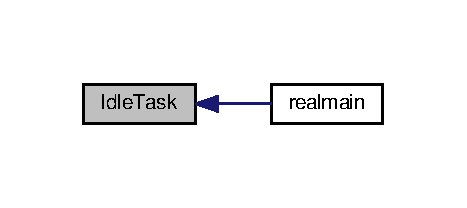
\includegraphics[width=224pt]{_lab5_8c_a269a2b542c489c0d00dd5d4328ed6ccf_icgraph}
\end{center}
\end{figure}


\hypertarget{_lab5_8c_a2e36aaea6b9cab2ca1faab2c2d760271}{\index{Lab5.\-c@{Lab5.\-c}!Interpreter@{Interpreter}}
\index{Interpreter@{Interpreter}!Lab5.c@{Lab5.\-c}}
\subsubsection[{Interpreter}]{\setlength{\rightskip}{0pt plus 5cm}void Interpreter (
\begin{DoxyParamCaption}
\item[{void}]{}
\end{DoxyParamCaption}
)}}\label{_lab5_8c_a2e36aaea6b9cab2ca1faab2c2d760271}


Definition at line 142 of file Lab5.\-c.


\begin{DoxyCode}
142                   \{
143   \textcolor{keywordtype}{char} buff[10];
144   printf(\textcolor{stringliteral}{">>\(\backslash\)n\(\backslash\)r"});
145   scanf(\textcolor{stringliteral}{"%s\(\backslash\)n"}, buff);
146   printf(\textcolor{stringliteral}{"%s\(\backslash\)n\(\backslash\)r"}, buff);
147 \}
\end{DoxyCode}


Here is the caller graph for this function\-:
\nopagebreak
\begin{figure}[H]
\begin{center}
\leavevmode
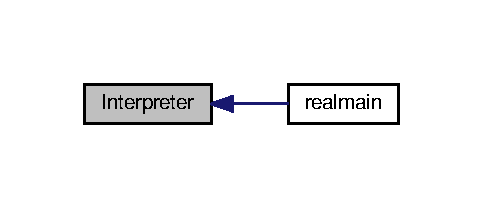
\includegraphics[width=232pt]{_lab5_8c_a2e36aaea6b9cab2ca1faab2c2d760271_icgraph}
\end{center}
\end{figure}


\hypertarget{_lab5_8c_a840291bc02cba5474a4cb46a9b9566fe}{\index{Lab5.\-c@{Lab5.\-c}!main@{main}}
\index{main@{main}!Lab5.c@{Lab5.\-c}}
\subsubsection[{main}]{\setlength{\rightskip}{0pt plus 5cm}int main (
\begin{DoxyParamCaption}
\item[{void}]{}
\end{DoxyParamCaption}
)}}\label{_lab5_8c_a840291bc02cba5474a4cb46a9b9566fe}


Definition at line 364 of file Lab5.\-c.


\begin{DoxyCode}
364               \{   \textcolor{comment}{// testmain1}
365   OS\_Init();           \textcolor{comment}{// initialize, disable interrupts}
366   \hyperlink{_lab5_8c_a5b51a90348618cbd5eb0e65114ea0daf}{PortE\_Init}();
367   \hyperlink{_lab5_8c_a1ef39ee2274d28bab6daa26359630c57}{PE3} = 0x00;
368 \textcolor{comment}{//*******attach background tasks***********}
369 \textcolor{comment}{//  OS\_AddPeriodicThread(&disk\_timerproc,10*TIME\_1MS,0);   // time out routines for disk}
370 \textcolor{comment}{//  OS\_AddButtonTask(&RunTest,2);}
371   
372   NumCreated = 0 ;
373 \textcolor{comment}{// create initial foreground threads}
374 \textcolor{comment}{//  NumCreated += OS\_AddThread(&TestFAT,128,1);  }
375   \textcolor{comment}{//NumCreated += OS\_AddThread(&IdleTask,128,3); }
376   NumCreated += OS\_AddThread(&\hyperlink{_lab5_8c_ad4c2bdb78f3b09301fc0a24bbc9d1a5d}{TestUs}, 128, 1);
377   \textcolor{comment}{//NumCreated += OS\_AddThread(&TestUs, 128, 1);}
378   OS\_Launch(10*TIME\_1MS); \textcolor{comment}{// doesn't return, interrupts enabled in here}
379   \textcolor{keywordflow}{return} 0;               \textcolor{comment}{// this never executes}
380 \}
\end{DoxyCode}


Here is the call graph for this function\-:
\nopagebreak
\begin{figure}[H]
\begin{center}
\leavevmode
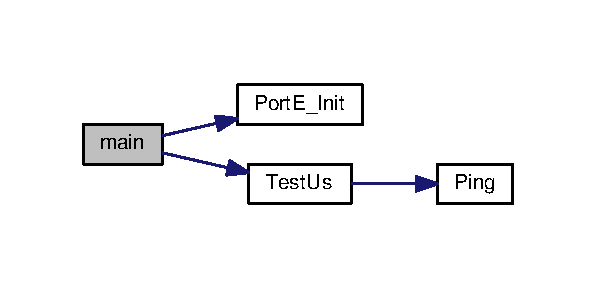
\includegraphics[width=286pt]{_lab5_8c_a840291bc02cba5474a4cb46a9b9566fe_cgraph}
\end{center}
\end{figure}


\hypertarget{_lab5_8c_a9c8a4d21a75e6a19ea31df0c5ccecfc2}{\index{Lab5.\-c@{Lab5.\-c}!Ping@{Ping}}
\index{Ping@{Ping}!Lab5.c@{Lab5.\-c}}
\subsubsection[{Ping}]{\setlength{\rightskip}{0pt plus 5cm}uint32\-\_\-t Ping (
\begin{DoxyParamCaption}
\item[{void}]{}
\end{DoxyParamCaption}
)}}\label{_lab5_8c_a9c8a4d21a75e6a19ea31df0c5ccecfc2}


Definition at line 299 of file Lab5.\-c.


\begin{DoxyCode}
299                    \{
300   uint32\_t pingStartTime; 
301   uint32\_t pingEndTime;
302   \textcolor{comment}{//Write GPIO\_Pin High}
303   \hyperlink{_lab5_8c_a1ef39ee2274d28bab6daa26359630c57}{PE3} = 0x08;
304   OS\_DelayUS(5);
305   \textcolor{comment}{//Write GPIO Pin Low}
306   \hyperlink{_lab5_8c_a1ef39ee2274d28bab6daa26359630c57}{PE3} = 0x00;
307   \textcolor{comment}{//Could move into a ISR}
308   \textcolor{comment}{//while(gpio\_Pin\_Low)\{\}}
309   \textcolor{comment}{//while(PE2 == 0)\{OS\_DelayUS(1);\}}
310   \textcolor{keywordflow}{while}(\hyperlink{_lab5_8c_ab9f47403c8a3489beafcac840b8fff7d}{PE2} == 0)\{\}
311   pingStartTime = OS\_GetUsTime();
312   \textcolor{comment}{//while(gpio\_Pin\_High)\{\}}
313   \textcolor{comment}{//while(PE2 != 0)\{OS\_DelayUS(1);\}}
314   \textcolor{keywordflow}{while}(\hyperlink{_lab5_8c_ab9f47403c8a3489beafcac840b8fff7d}{PE2} != 0)\{\}
315 \textcolor{comment}{//  OS\_DelayUS(18500); //For Simulation}
316 
317   pingEndTime = OS\_GetUsTime();
318   OS\_DelayUS(200);
319   \textcolor{comment}{//Speed of sound in air is approx c = 343 m/s = 340 m/s * 1000m.0m/m * (1s/100000us)}
320   \textcolor{comment}{//Then the ping time is c*dT/2}
321   \textcolor{keywordflow}{return} ((pingEndTime - pingStartTime) \textcolor{comment}{/*>> 1*/})*34300/1000000;
322   \textcolor{comment}{//return (uint32\_t)(((float)((pingEndTime - pingStartTime) >> 1))*34000.0/1000000.0);}
323 \}
\end{DoxyCode}


Here is the caller graph for this function\-:
\nopagebreak
\begin{figure}[H]
\begin{center}
\leavevmode
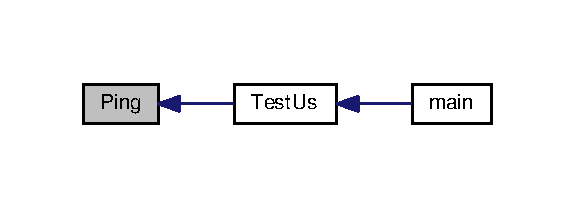
\includegraphics[width=276pt]{_lab5_8c_a9c8a4d21a75e6a19ea31df0c5ccecfc2_icgraph}
\end{center}
\end{figure}


\hypertarget{_lab5_8c_a5b51a90348618cbd5eb0e65114ea0daf}{\index{Lab5.\-c@{Lab5.\-c}!Port\-E\-\_\-\-Init@{Port\-E\-\_\-\-Init}}
\index{Port\-E\-\_\-\-Init@{Port\-E\-\_\-\-Init}!Lab5.c@{Lab5.\-c}}
\subsubsection[{Port\-E\-\_\-\-Init}]{\setlength{\rightskip}{0pt plus 5cm}void Port\-E\-\_\-\-Init (
\begin{DoxyParamCaption}
\item[{void}]{}
\end{DoxyParamCaption}
)}}\label{_lab5_8c_a5b51a90348618cbd5eb0e65114ea0daf}


Definition at line 37 of file Lab5.\-c.


\begin{DoxyCode}
37                      \{ \textcolor{keywordtype}{unsigned} \textcolor{keywordtype}{long} \textcolor{keyword}{volatile} delay;
38   \textcolor{comment}{//SYSCTL\_RCGC2\_R |= 0x10;       // activate port E}
39   SYSCTL\_RCGCGPIO\_R |= 0x10;       
40   delay = SYSCTL\_RCGC2\_R;        
41   delay = SYSCTL\_RCGC2\_R;         
42   GPIO\_PORTE\_DIR\_R |= 0x0F;    \textcolor{comment}{// make PE3-0 output heartbeats}
43   GPIO\_PORTE\_DIR\_R &= ~0x04;
44   GPIO\_PORTE\_AFSEL\_R &= ~0x0F;   \textcolor{comment}{// disable alt funct on PE3-0}
45   GPIO\_PORTE\_DEN\_R |= 0x0F;     \textcolor{comment}{// enable digital I/O on PE3-0}
46   GPIO\_PORTE\_PCTL\_R = ~0x0000FFFF;
47   GPIO\_PORTE\_AMSEL\_R &= ~0x0F;;      \textcolor{comment}{// disable analog functionality on PF}
48 \}
\end{DoxyCode}


Here is the caller graph for this function\-:
\nopagebreak
\begin{figure}[H]
\begin{center}
\leavevmode
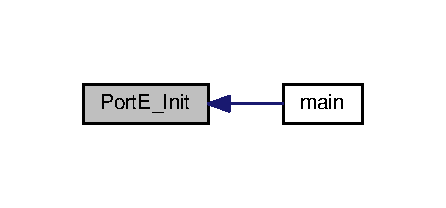
\includegraphics[width=214pt]{_lab5_8c_a5b51a90348618cbd5eb0e65114ea0daf_icgraph}
\end{center}
\end{figure}


\hypertarget{_lab5_8c_a7eaf80f6bdd1fd573219220dbb7f8837}{\index{Lab5.\-c@{Lab5.\-c}!Producer@{Producer}}
\index{Producer@{Producer}!Lab5.c@{Lab5.\-c}}
\subsubsection[{Producer}]{\setlength{\rightskip}{0pt plus 5cm}void Producer (
\begin{DoxyParamCaption}
\item[{unsigned long}]{data}
\end{DoxyParamCaption}
)}}\label{_lab5_8c_a7eaf80f6bdd1fd573219220dbb7f8837}


Definition at line 113 of file Lab5.\-c.


\begin{DoxyCode}
113                                  \{  
114   \textcolor{keywordflow}{if}(\hyperlink{_lab5_8c_a1e26c569f8ea4c8145952219697f181f}{Running})\{
115     \textcolor{keywordflow}{if}(OS\_Fifo\_Put(data))\{     \textcolor{comment}{// send to Robot}
116       NumSamples++;
117     \} \textcolor{keywordflow}{else}\{ 
118       DataLost++;
119     \} 
120   \}
121 \}
\end{DoxyCode}


Here is the caller graph for this function\-:
\nopagebreak
\begin{figure}[H]
\begin{center}
\leavevmode
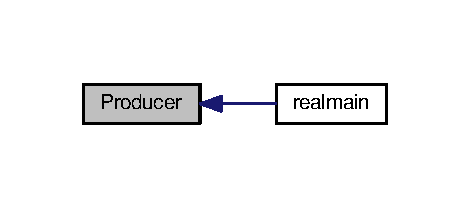
\includegraphics[width=226pt]{_lab5_8c_a7eaf80f6bdd1fd573219220dbb7f8837_icgraph}
\end{center}
\end{figure}


\hypertarget{_lab5_8c_a7eff0fb752de46f3df0342f22f69c458}{\index{Lab5.\-c@{Lab5.\-c}!realmain@{realmain}}
\index{realmain@{realmain}!Lab5.c@{Lab5.\-c}}
\subsubsection[{realmain}]{\setlength{\rightskip}{0pt plus 5cm}int realmain (
\begin{DoxyParamCaption}
\item[{void}]{}
\end{DoxyParamCaption}
)}}\label{_lab5_8c_a7eff0fb752de46f3df0342f22f69c458}


Definition at line 156 of file Lab5.\-c.


\begin{DoxyCode}
156                   \{        \textcolor{comment}{// lab 5 real main}
157   OS\_Init();           \textcolor{comment}{// initialize, disable interrupts}
158   \hyperlink{_lab5_8c_a1e26c569f8ea4c8145952219697f181f}{Running} = 0;         \textcolor{comment}{// robot not running}
159   DataLost = 0;        \textcolor{comment}{// lost data between producer and consumer}
160   NumSamples = 0;
161 
162 \textcolor{comment}{//********initialize communication channels}
163   OS\_Fifo\_Init(512);    \textcolor{comment}{// ***note*** 4 is not big enough*****}
164   \hyperlink{_a_d_c_8c_a9fdea7e06f4c4769ab22981dafb58477}{ADC\_Collect}(0, 1000, &\hyperlink{_lab5_8c_a7eaf80f6bdd1fd573219220dbb7f8837}{Producer}); \textcolor{comment}{// start ADC sampling, channel 0, 1000 Hz}
165 
166 \textcolor{comment}{//*******attach background tasks***********}
167 \textcolor{comment}{//  OS\_AddButtonTask(&ButtonPush,2);}
168 \textcolor{comment}{//  OS\_AddButtonTask(&DownPush,3);}
169   OS\_AddPeriodicThread(disk\_timerproc,10*TIME\_1MS,5);
170 
171   NumCreated = 0 ;
172 \textcolor{comment}{// create initial foreground threads}
173   NumCreated += OS\_AddThread(&\hyperlink{_lab5_8c_a2e36aaea6b9cab2ca1faab2c2d760271}{Interpreter},128,2); 
174   NumCreated += OS\_AddThread(&\hyperlink{_lab5_8c_a269a2b542c489c0d00dd5d4328ed6ccf}{IdleTask},128,7);  \textcolor{comment}{// runs when nothing useful to do}
175  
176   OS\_Launch(\hyperlink{_lab5_8c_ae586204918bfbea259810829a239d886}{TIMESLICE}); \textcolor{comment}{// doesn't return, interrupts enabled in here}
177   \textcolor{keywordflow}{return} 0;             \textcolor{comment}{// this never executes}
178 \}
\end{DoxyCode}


Here is the call graph for this function\-:
\nopagebreak
\begin{figure}[H]
\begin{center}
\leavevmode
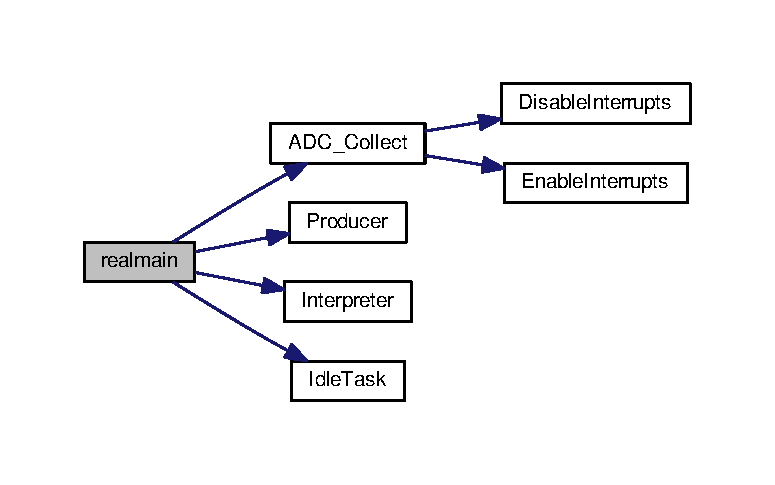
\includegraphics[width=350pt]{_lab5_8c_a7eff0fb752de46f3df0342f22f69c458_cgraph}
\end{center}
\end{figure}


\hypertarget{_lab5_8c_aefdc786873bfd8245aa0f47e54f3077e}{\index{Lab5.\-c@{Lab5.\-c}!Robot@{Robot}}
\index{Robot@{Robot}!Lab5.c@{Lab5.\-c}}
\subsubsection[{Robot}]{\setlength{\rightskip}{0pt plus 5cm}void Robot (
\begin{DoxyParamCaption}
\item[{void}]{}
\end{DoxyParamCaption}
)}}\label{_lab5_8c_aefdc786873bfd8245aa0f47e54f3077e}


Definition at line 62 of file Lab5.\-c.


\begin{DoxyCode}
62                 \{   
63 \textcolor{keywordtype}{unsigned} \textcolor{keywordtype}{long} data;      \textcolor{comment}{// ADC sample, 0 to 1023}
64 \textcolor{keywordtype}{unsigned} \textcolor{keywordtype}{long} voltage;   \textcolor{comment}{// in mV,      0 to 3000}
65 \textcolor{keywordtype}{unsigned} \textcolor{keywordtype}{long} time;      \textcolor{comment}{// in 10msec,  0 to 1000 }
66 \textcolor{keywordtype}{unsigned} \textcolor{keywordtype}{long} t=0;
67   OS\_ClearMsTime();    
68   DataLost = 0;          \textcolor{comment}{// new run with no lost data }
69   printf(\textcolor{stringliteral}{"Robot running..."});
70   eFile\_RedirectToFile(\textcolor{stringliteral}{"Robot"});
71   printf(\textcolor{stringliteral}{"time(sec)\(\backslash\)tdata(volts)\(\backslash\)n\(\backslash\)r"});
72   \textcolor{keywordflow}{do}\{
73     t++;
74     time=OS\_MsTime();            \textcolor{comment}{// 10ms resolution in this OS}
75     data = OS\_Fifo\_Get();        \textcolor{comment}{// 1000 Hz sampling get from producer}
76     voltage = (300*data)/1024;   \textcolor{comment}{// in mV}
77     printf(\textcolor{stringliteral}{"%0u.%02u\(\backslash\)t%0u.%03u\(\backslash\)n\(\backslash\)r"},time/100,time%100,voltage/1000,voltage%1000);
78   \}
79   \textcolor{keywordflow}{while}(time < 1000);       \textcolor{comment}{// change this to mean 10 seconds}
80   eFile\_EndRedirectToFile();
81   printf(\textcolor{stringliteral}{"done.\(\backslash\)n\(\backslash\)r"});
82   \hyperlink{_lab5_8c_a1e26c569f8ea4c8145952219697f181f}{Running} = 0;                \textcolor{comment}{// robot no longer running}
83   OS\_Kill();
84 \}
\end{DoxyCode}


Here is the caller graph for this function\-:
\nopagebreak
\begin{figure}[H]
\begin{center}
\leavevmode
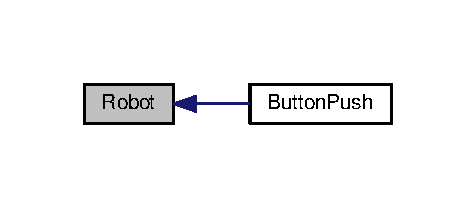
\includegraphics[width=228pt]{_lab5_8c_aefdc786873bfd8245aa0f47e54f3077e_icgraph}
\end{center}
\end{figure}


\hypertarget{_lab5_8c_a8ae9923a4397b1cc33baf08ea2341c33}{\index{Lab5.\-c@{Lab5.\-c}!Run\-Test@{Run\-Test}}
\index{Run\-Test@{Run\-Test}!Lab5.c@{Lab5.\-c}}
\subsubsection[{Run\-Test}]{\setlength{\rightskip}{0pt plus 5cm}void Run\-Test (
\begin{DoxyParamCaption}
\item[{void}]{}
\end{DoxyParamCaption}
)}}\label{_lab5_8c_a8ae9923a4397b1cc33baf08ea2341c33}


Definition at line 222 of file Lab5.\-c.


\begin{DoxyCode}
222                   \{
223   NumCreated += OS\_AddThread(&\hyperlink{_lab5_8c_a3efcf5e79ed9738d40e3dbaf3befc678}{TestDisk},128,1);  
224 \}
\end{DoxyCode}


Here is the call graph for this function\-:
\nopagebreak
\begin{figure}[H]
\begin{center}
\leavevmode
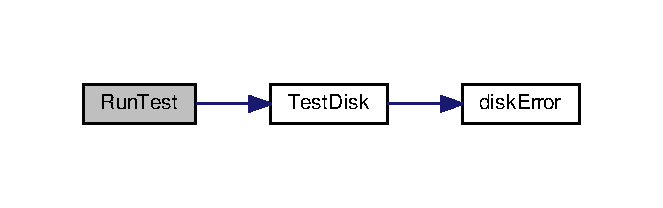
\includegraphics[width=318pt]{_lab5_8c_a8ae9923a4397b1cc33baf08ea2341c33_cgraph}
\end{center}
\end{figure}


\hypertarget{_lab5_8c_a3efcf5e79ed9738d40e3dbaf3befc678}{\index{Lab5.\-c@{Lab5.\-c}!Test\-Disk@{Test\-Disk}}
\index{Test\-Disk@{Test\-Disk}!Lab5.c@{Lab5.\-c}}
\subsubsection[{Test\-Disk}]{\setlength{\rightskip}{0pt plus 5cm}void Test\-Disk (
\begin{DoxyParamCaption}
\item[{void}]{}
\end{DoxyParamCaption}
)}}\label{_lab5_8c_a3efcf5e79ed9738d40e3dbaf3befc678}


Definition at line 189 of file Lab5.\-c.


\begin{DoxyCode}
189                    \{  DSTATUS result;  \textcolor{keywordtype}{unsigned} \textcolor{keywordtype}{short} block;  \textcolor{keywordtype}{int} i; \textcolor{keywordtype}{unsigned} \textcolor{keywordtype}{long} n;
190   \textcolor{comment}{// simple test of eDisk}
191   printf(\textcolor{stringliteral}{"\(\backslash\)n\(\backslash\)rEE345M/EE380L, Lab 5 eDisk test\(\backslash\)n\(\backslash\)r"});
192   result = eDisk\_Init(0);  \textcolor{comment}{// initialize disk}
193   \textcolor{keywordflow}{if}(result) \hyperlink{_lab5_8c_a22c9a06aa7985e858ece98451d29d482}{diskError}(\textcolor{stringliteral}{"eDisk\_Init"},result);
194   printf(\textcolor{stringliteral}{"Writing blocks\(\backslash\)n\(\backslash\)r"});
195   n = 1;    \textcolor{comment}{// seed}
196   \textcolor{keywordflow}{for}(block = 0; block < \hyperlink{_lab5_8c_a02723c1cf9784c591e45af7bf584f97c}{MAXBLOCKS}; block++)\{
197     \textcolor{keywordflow}{for}(i=0;i<512;i++)\{
198       n = (16807*n)%2147483647; \textcolor{comment}{// pseudo random sequence}
199       \hyperlink{_lab5_8c_a9516ea594e030f96eb9483d95f1583a5}{buffer}[i] = 0xFF&n;        
200     \}
201     \hyperlink{_lab5_8c_aab864bd67f4cea10fd17ee13808668cd}{GPIO\_PF3} = 0x08;     \textcolor{comment}{// PF3 high for 100 block writes}
202     \textcolor{keywordflow}{if}(eDisk\_WriteBlock(\hyperlink{_lab5_8c_a9516ea594e030f96eb9483d95f1583a5}{buffer},block))\hyperlink{_lab5_8c_a22c9a06aa7985e858ece98451d29d482}{diskError}(\textcolor{stringliteral}{"eDisk\_WriteBlock"},block); \textcolor{comment}{// save to disk}
203     \hyperlink{_lab5_8c_aab864bd67f4cea10fd17ee13808668cd}{GPIO\_PF3} = 0x00;     
204   \}  
205   printf(\textcolor{stringliteral}{"Reading blocks\(\backslash\)n\(\backslash\)r"});
206   n = 1;  \textcolor{comment}{// reseed, start over to get the same sequence}
207   \textcolor{keywordflow}{for}(block = 0; block < \hyperlink{_lab5_8c_a02723c1cf9784c591e45af7bf584f97c}{MAXBLOCKS}; block++)\{
208     \hyperlink{_lab5_8c_a959a99608831fef309047e405b5059bc}{GPIO\_PF2} = 0x04;     \textcolor{comment}{// PF2 high for one block read}
209     \textcolor{keywordflow}{if}(eDisk\_ReadBlock(\hyperlink{_lab5_8c_a9516ea594e030f96eb9483d95f1583a5}{buffer},block))\hyperlink{_lab5_8c_a22c9a06aa7985e858ece98451d29d482}{diskError}(\textcolor{stringliteral}{"eDisk\_ReadBlock"},block); \textcolor{comment}{// read from disk}
210     \hyperlink{_lab5_8c_a959a99608831fef309047e405b5059bc}{GPIO\_PF2} = 0x00;
211     \textcolor{keywordflow}{for}(i=0;i<512;i++)\{
212       n = (16807*n)%2147483647; \textcolor{comment}{// pseudo random sequence}
213       \textcolor{keywordflow}{if}(\hyperlink{_lab5_8c_a9516ea594e030f96eb9483d95f1583a5}{buffer}[i] != (0xFF&n))\{
214         printf(\textcolor{stringliteral}{"Read data not correct, block=%u, i=%u, expected %u, read %u\(\backslash\)n\(\backslash\)r"},block,i,(0xFF&n),
      \hyperlink{_lab5_8c_a9516ea594e030f96eb9483d95f1583a5}{buffer}[i]);
215         OS\_Kill();
216       \}      
217     \}
218   \}  
219   printf(\textcolor{stringliteral}{"Successful test of %u blocks\(\backslash\)n\(\backslash\)r"},MAXBLOCKS);
220   OS\_Kill();
221 \}
\end{DoxyCode}


Here is the call graph for this function\-:
\nopagebreak
\begin{figure}[H]
\begin{center}
\leavevmode
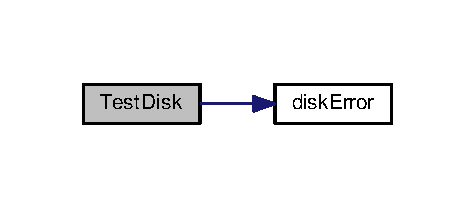
\includegraphics[width=228pt]{_lab5_8c_a3efcf5e79ed9738d40e3dbaf3befc678_cgraph}
\end{center}
\end{figure}




Here is the caller graph for this function\-:
\nopagebreak
\begin{figure}[H]
\begin{center}
\leavevmode
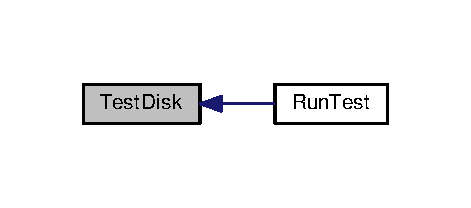
\includegraphics[width=226pt]{_lab5_8c_a3efcf5e79ed9738d40e3dbaf3befc678_icgraph}
\end{center}
\end{figure}


\hypertarget{_lab5_8c_aad6d0bf2cbb02582664e1107ccee3483}{\index{Lab5.\-c@{Lab5.\-c}!Test\-F\-A\-T@{Test\-F\-A\-T}}
\index{Test\-F\-A\-T@{Test\-F\-A\-T}!Lab5.c@{Lab5.\-c}}
\subsubsection[{Test\-F\-A\-T}]{\setlength{\rightskip}{0pt plus 5cm}void Test\-F\-A\-T (
\begin{DoxyParamCaption}
\item[{void}]{}
\end{DoxyParamCaption}
)}}\label{_lab5_8c_aad6d0bf2cbb02582664e1107ccee3483}


Definition at line 290 of file Lab5.\-c.


\begin{DoxyCode}
290                   \{
291   \textcolor{comment}{// simple test of eDisk}
292   eFile\_Init();
293   printf(\textcolor{stringliteral}{"\(\backslash\)n\(\backslash\)rEE345M/EE380L, Lab 5 eDisk test\(\backslash\)n\(\backslash\)r"});
294 
295   printf(\textcolor{stringliteral}{"Successful test of %u blocks\(\backslash\)n\(\backslash\)r"},\hyperlink{_lab5_8c_a02723c1cf9784c591e45af7bf584f97c}{MAXBLOCKS});
296   OS\_Kill();
297 \}
\end{DoxyCode}
\hypertarget{_lab5_8c_a95d7d847e2c29bc8c83224318399d41b}{\index{Lab5.\-c@{Lab5.\-c}!Test\-File@{Test\-File}}
\index{Test\-File@{Test\-File}!Lab5.c@{Lab5.\-c}}
\subsubsection[{Test\-File}]{\setlength{\rightskip}{0pt plus 5cm}void Test\-File (
\begin{DoxyParamCaption}
\item[{void}]{}
\end{DoxyParamCaption}
)}}\label{_lab5_8c_a95d7d847e2c29bc8c83224318399d41b}


Definition at line 245 of file Lab5.\-c.


\begin{DoxyCode}
245                    \{   \textcolor{keywordtype}{int} i; \textcolor{keywordtype}{char} data; 
246   printf(\textcolor{stringliteral}{"\(\backslash\)n\(\backslash\)rEE345M/EE380L, Lab 5 eFile test\(\backslash\)n\(\backslash\)r"});
247   \textcolor{comment}{// simple test of eFile}
248   \textcolor{keywordflow}{if}(eFile\_Init())              \hyperlink{_lab5_8c_a22c9a06aa7985e858ece98451d29d482}{diskError}(\textcolor{stringliteral}{"eFile\_Init"},0); 
249   \textcolor{keywordflow}{if}(eFile\_Format())            \hyperlink{_lab5_8c_a22c9a06aa7985e858ece98451d29d482}{diskError}(\textcolor{stringliteral}{"eFile\_Format"},0); 
250 \textcolor{comment}{//  eFile\_Directory(&Serial\_OutChar);}
251   \textcolor{keywordflow}{if}(eFile\_Create(\textcolor{stringliteral}{"file1"}))     \hyperlink{_lab5_8c_a22c9a06aa7985e858ece98451d29d482}{diskError}(\textcolor{stringliteral}{"eFile\_Create"},0);
252   \textcolor{keywordflow}{if}(eFile\_WOpen(\textcolor{stringliteral}{"file1"}))      \hyperlink{_lab5_8c_a22c9a06aa7985e858ece98451d29d482}{diskError}(\textcolor{stringliteral}{"eFile\_WOpen"},0);
253   \textcolor{keywordflow}{for}(i=0;i<1000;i++)\{
254     \textcolor{keywordflow}{if}(eFile\_Write(\textcolor{charliteral}{'a'}+i%26))   \hyperlink{_lab5_8c_a22c9a06aa7985e858ece98451d29d482}{diskError}(\textcolor{stringliteral}{"eFile\_Write"},i);
255     \textcolor{keywordflow}{if}(i%52==51)\{
256       \textcolor{keywordflow}{if}(eFile\_Write(\textcolor{charliteral}{'\(\backslash\)n'}))     \hyperlink{_lab5_8c_a22c9a06aa7985e858ece98451d29d482}{diskError}(\textcolor{stringliteral}{"eFile\_Write"},i);  
257       \textcolor{keywordflow}{if}(eFile\_Write(\textcolor{charliteral}{'\(\backslash\)r'}))     \hyperlink{_lab5_8c_a22c9a06aa7985e858ece98451d29d482}{diskError}(\textcolor{stringliteral}{"eFile\_Write"},i);
258     \}
259   \}
260   \textcolor{keywordflow}{if}(eFile\_WClose())            \hyperlink{_lab5_8c_a22c9a06aa7985e858ece98451d29d482}{diskError}(\textcolor{stringliteral}{"eFile\_Close"},0);
261 \textcolor{comment}{//  eFile\_Directory(&Serial\_OutChar);}
262   \textcolor{keywordflow}{if}(eFile\_ROpen(\textcolor{stringliteral}{"file1"}))      \hyperlink{_lab5_8c_a22c9a06aa7985e858ece98451d29d482}{diskError}(\textcolor{stringliteral}{"eFile\_ROpen"},0);
263   \textcolor{keywordflow}{for}(i=0;i<1000;i++)\{
264     \textcolor{keywordflow}{if}(eFile\_ReadNext(&data))   \hyperlink{_lab5_8c_a22c9a06aa7985e858ece98451d29d482}{diskError}(\textcolor{stringliteral}{"eFile\_ReadNext"},i);
265 \textcolor{comment}{//    Serial\_OutChar(data);}
266   \}
267   \textcolor{keywordflow}{if}(eFile\_Delete(\textcolor{stringliteral}{"file1"}))     \hyperlink{_lab5_8c_a22c9a06aa7985e858ece98451d29d482}{diskError}(\textcolor{stringliteral}{"eFile\_Delete"},0);
268 \textcolor{comment}{//  eFile\_Directory(&Serial\_OutChar);}
269   printf(\textcolor{stringliteral}{"Successful test of creating a file\(\backslash\)n\(\backslash\)r"});
270   OS\_Kill();
271 \}
\end{DoxyCode}


Here is the call graph for this function\-:
\nopagebreak
\begin{figure}[H]
\begin{center}
\leavevmode
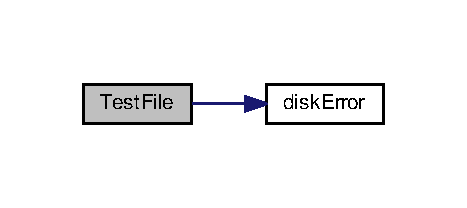
\includegraphics[width=224pt]{_lab5_8c_a95d7d847e2c29bc8c83224318399d41b_cgraph}
\end{center}
\end{figure}




Here is the caller graph for this function\-:
\nopagebreak
\begin{figure}[H]
\begin{center}
\leavevmode
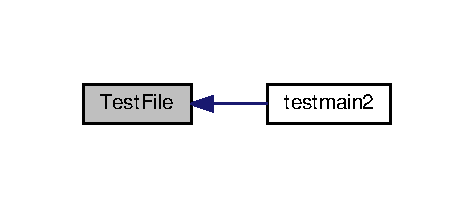
\includegraphics[width=228pt]{_lab5_8c_a95d7d847e2c29bc8c83224318399d41b_icgraph}
\end{center}
\end{figure}


\hypertarget{_lab5_8c_abbcfdc8ab315a9f273a0c498a0e73e29}{\index{Lab5.\-c@{Lab5.\-c}!testmain2@{testmain2}}
\index{testmain2@{testmain2}!Lab5.c@{Lab5.\-c}}
\subsubsection[{testmain2}]{\setlength{\rightskip}{0pt plus 5cm}int testmain2 (
\begin{DoxyParamCaption}
\item[{void}]{}
\end{DoxyParamCaption}
)}}\label{_lab5_8c_abbcfdc8ab315a9f273a0c498a0e73e29}


Definition at line 276 of file Lab5.\-c.


\begin{DoxyCode}
276                    \{ 
277   OS\_Init();           \textcolor{comment}{// initialize, disable interrupts}
278 
279 \textcolor{comment}{//*******attach background tasks***********}
280   OS\_AddPeriodicThread(&disk\_timerproc,10*TIME\_1MS,0);   \textcolor{comment}{// time out routines for disk}
281   
282   NumCreated = 0 ;
283 \textcolor{comment}{// create initial foreground threads}
284   NumCreated += OS\_AddThread(&\hyperlink{_lab5_8c_a95d7d847e2c29bc8c83224318399d41b}{TestFile},128,1);  
285   \textcolor{comment}{//NumCreated += OS\_AddThread(&IdleTask,128,3); }
286  
287   OS\_Launch(10*TIME\_1MS); \textcolor{comment}{// doesn't return, interrupts enabled in here}
288   \textcolor{keywordflow}{return} 0;               \textcolor{comment}{// this never executes}
289 \}
\end{DoxyCode}


Here is the call graph for this function\-:
\nopagebreak
\begin{figure}[H]
\begin{center}
\leavevmode
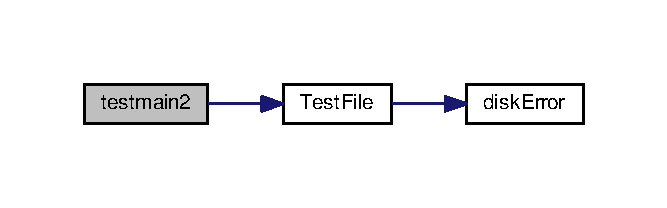
\includegraphics[width=320pt]{_lab5_8c_abbcfdc8ab315a9f273a0c498a0e73e29_cgraph}
\end{center}
\end{figure}


\hypertarget{_lab5_8c_ad4c2bdb78f3b09301fc0a24bbc9d1a5d}{\index{Lab5.\-c@{Lab5.\-c}!Test\-Us@{Test\-Us}}
\index{Test\-Us@{Test\-Us}!Lab5.c@{Lab5.\-c}}
\subsubsection[{Test\-Us}]{\setlength{\rightskip}{0pt plus 5cm}void Test\-Us (
\begin{DoxyParamCaption}
\item[{void}]{}
\end{DoxyParamCaption}
)}}\label{_lab5_8c_ad4c2bdb78f3b09301fc0a24bbc9d1a5d}


Definition at line 324 of file Lab5.\-c.


\begin{DoxyCode}
324                  \{
325   
326   uint32\_t currTime; 
327   uint32\_t currTime2;
328   uint32\_t distance;
329   \textcolor{comment}{//uint32\_t distance\_buff[4];}
330   \textcolor{keywordtype}{unsigned} \textcolor{keywordtype}{long} \textcolor{keywordtype}{id} = OS\_Id();
331   uint32\_t i = 0;
332   uint32\_t x = 5;
333   x--;
334   x--;
335   x--;
336   currTime = OS\_GetUsTime();
337   OS\_DelayUS(5);
338   currTime2 = OS\_GetUsTime();
339   printf(\textcolor{stringliteral}{"Verifying Timing Conditions\(\backslash\)n"});
340   printf(\textcolor{stringliteral}{"%u\(\backslash\)t%u\(\backslash\)t%u\(\backslash\)n"}, currTime, currTime2, currTime2-currTime);
341   
342   currTime = OS\_GetUsTime();
343   currTime2 = OS\_GetUsTime();
344   printf(\textcolor{stringliteral}{"Verifying Timing Conditions\(\backslash\)n"});
345   printf(\textcolor{stringliteral}{"%u\(\backslash\)t%u\(\backslash\)t%u\(\backslash\)n"}, currTime, currTime2, currTime2-currTime);
346   
347     currTime = OS\_GetUsTime();
348     currTime2 = OS\_GetUsTime();
349     printf(\textcolor{stringliteral}{"Verifying Timing Conditions\(\backslash\)n"});
350     printf(\textcolor{stringliteral}{"%u\(\backslash\)t%u\(\backslash\)t%u\(\backslash\)n"}, currTime, currTime2, currTime2-currTime);
351   \textcolor{keywordflow}{while}(1)\{
352     distance = 0;
353     \textcolor{keywordflow}{for}(i = 0; i < 4; i++)\{
354       currTime = OS\_GetUsTime();
355       \textcolor{comment}{//distance\_buff[i] = Ping();}
356       distance += \hyperlink{_lab5_8c_a9c8a4d21a75e6a19ea31df0c5ccecfc2}{Ping}();
357       currTime2 = OS\_GetUsTime();
358     \}
359     distance = distance >> 2;
360     printf(\textcolor{stringliteral}{"ID: %u\(\backslash\)t\(\backslash\)t%u\(\backslash\)t\(\backslash\)t%u\(\backslash\)n\(\backslash\)r"}, \textcolor{keywordtype}{id}, distance, currTime2-currTime);
361   \}
362   OS\_Kill();
363 \}
\end{DoxyCode}


Here is the call graph for this function\-:
\nopagebreak
\begin{figure}[H]
\begin{center}
\leavevmode
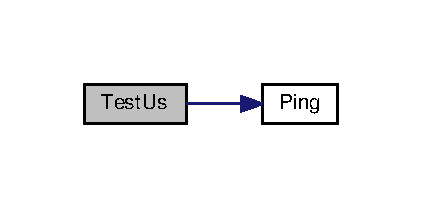
\includegraphics[width=202pt]{_lab5_8c_ad4c2bdb78f3b09301fc0a24bbc9d1a5d_cgraph}
\end{center}
\end{figure}




Here is the caller graph for this function\-:
\nopagebreak
\begin{figure}[H]
\begin{center}
\leavevmode
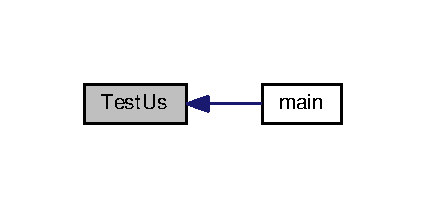
\includegraphics[width=204pt]{_lab5_8c_ad4c2bdb78f3b09301fc0a24bbc9d1a5d_icgraph}
\end{center}
\end{figure}




\subsection{Variable Documentation}
\hypertarget{_lab5_8c_a9516ea594e030f96eb9483d95f1583a5}{\index{Lab5.\-c@{Lab5.\-c}!buffer@{buffer}}
\index{buffer@{buffer}!Lab5.c@{Lab5.\-c}}
\subsubsection[{buffer}]{\setlength{\rightskip}{0pt plus 5cm}unsigned char buffer\mbox{[}512\mbox{]}}}\label{_lab5_8c_a9516ea594e030f96eb9483d95f1583a5}


Definition at line 182 of file Lab5.\-c.

\hypertarget{_lab5_8c_a1bb5d517b380a841c91444d3bbffb9ab}{\index{Lab5.\-c@{Lab5.\-c}!Idlecount@{Idlecount}}
\index{Idlecount@{Idlecount}!Lab5.c@{Lab5.\-c}}
\subsubsection[{Idlecount}]{\setlength{\rightskip}{0pt plus 5cm}unsigned long Idlecount =0}}\label{_lab5_8c_a1bb5d517b380a841c91444d3bbffb9ab}


Definition at line 128 of file Lab5.\-c.

\hypertarget{_lab5_8c_a1e26c569f8ea4c8145952219697f181f}{\index{Lab5.\-c@{Lab5.\-c}!Running@{Running}}
\index{Running@{Running}!Lab5.c@{Lab5.\-c}}
\subsubsection[{Running}]{\setlength{\rightskip}{0pt plus 5cm}int Running}}\label{_lab5_8c_a1e26c569f8ea4c8145952219697f181f}


Definition at line 23 of file Lab5.\-c.


\hypertarget{_lab6_8c}{\section{Lab6.\-c File Reference}
\label{_lab6_8c}\index{Lab6.\-c@{Lab6.\-c}}
}
{\ttfamily \#include $<$stdio.\-h$>$}\\*
{\ttfamily \#include $<$string.\-h$>$}\\*
{\ttfamily \#include \char`\"{}inc/hw\-\_\-types.\-h\char`\"{}}\\*
{\ttfamily \#include \char`\"{}A\-D\-C.\-h\char`\"{}}\\*
{\ttfamily \#include \char`\"{}os.\-h\char`\"{}}\\*
{\ttfamily \#include \char`\"{}inc/tm4c123gh6pm.\-h\char`\"{}}\\*
{\ttfamily \#include \char`\"{}Perf.\-h\char`\"{}}\\*
{\ttfamily \#include \char`\"{}can0.\-h\char`\"{}}\\*
{\ttfamily \#include \char`\"{}median.\-h\char`\"{}}\\*
{\ttfamily \#include \char`\"{}P\-W\-M\-Dual.\-h\char`\"{}}\\*
{\ttfamily \#include \char`\"{}Mailbox.\-hpp\char`\"{}}\\*
Include dependency graph for Lab6.\-c\-:
\nopagebreak
\begin{figure}[H]
\begin{center}
\leavevmode
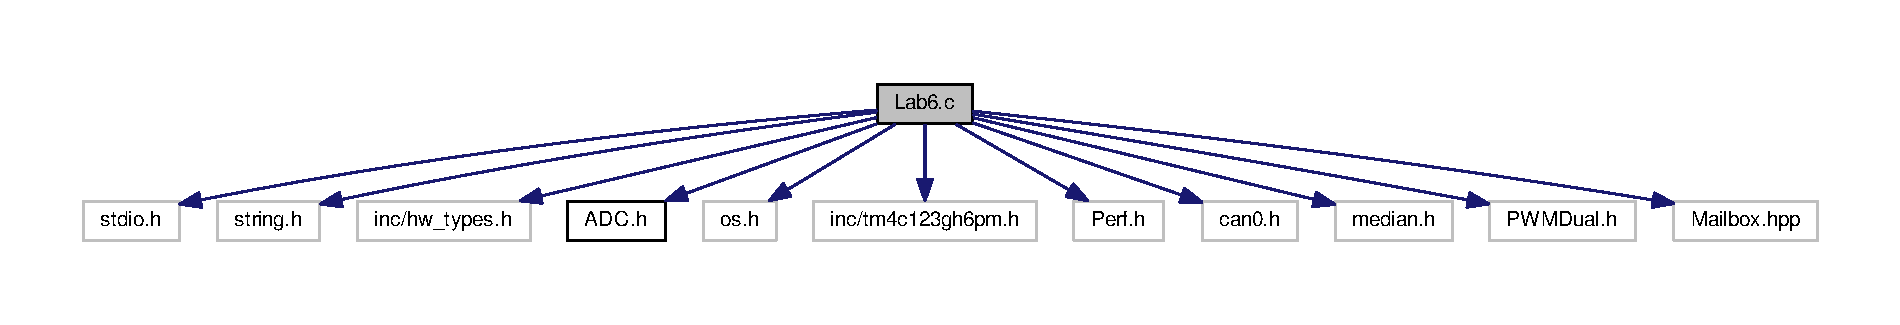
\includegraphics[width=350pt]{_lab6_8c__incl}
\end{center}
\end{figure}
\subsection*{Macros}
\begin{DoxyCompactItemize}
\item 
\#define \hyperlink{_lab6_8c_a90bf9206ca8b60d62247464501fb9e89}{Too\-Close}~1200
\item 
\#define \hyperlink{_lab6_8c_a930f8223aa964823168d8f4cf7418e44}{Too\-Far}~600
\item 
\#define \hyperlink{_lab6_8c_a084f0cbd524691ad1a56acf4e2858259}{Ok\-Range\-Min}~600
\item 
\#define \hyperlink{_lab6_8c_a45c01d393beae01b562c5cb6c26cc8ea}{Ok\-Range\-Max}~1200
\item 
\#define \hyperlink{_lab6_8c_ae586204918bfbea259810829a239d886}{T\-I\-M\-E\-S\-L\-I\-C\-E}~2$\ast$T\-I\-M\-E\-\_\-1\-M\-S
\item 
\#define \hyperlink{_lab6_8c_ab527c0e4b7c318dbae300412b03eed17}{G\-P\-I\-O\-\_\-\-P\-F0}~($\ast$((volatile unsigned long $\ast$)0x40025004))
\item 
\#define \hyperlink{_lab6_8c_abbb42535d15ee2366af5a5b1e2124a05}{G\-P\-I\-O\-\_\-\-P\-F1}~($\ast$((volatile unsigned long $\ast$)0x40025008))
\item 
\#define \hyperlink{_lab6_8c_a959a99608831fef309047e405b5059bc}{G\-P\-I\-O\-\_\-\-P\-F2}~($\ast$((volatile unsigned long $\ast$)0x40025010))
\item 
\#define \hyperlink{_lab6_8c_aab864bd67f4cea10fd17ee13808668cd}{G\-P\-I\-O\-\_\-\-P\-F3}~($\ast$((volatile unsigned long $\ast$)0x40025020))
\item 
\#define \hyperlink{_lab6_8c_a66dc5c770ec2c27da7ecceb303354ff4}{G\-P\-I\-O\-\_\-\-P\-G1}~($\ast$((volatile unsigned long $\ast$)0x40026008))
\item 
\#define \hyperlink{_lab6_8c_aa1bdfe98b68dc6bf0934403577a69402}{P\-D6}~($\ast$((volatile unsigned long $\ast$)0x40007100))
\item 
\#define \hyperlink{_lab6_8c_a3e427eea4be9cc64631d579b0d4c13ce}{P\-D7}~($\ast$((volatile unsigned long $\ast$)0x40007200))
\item 
\#define \hyperlink{_lab6_8c_aea08c09063c5962f8f60044f1829d54c}{P\-C6}~($\ast$((volatile unsigned long $\ast$)0x40006100))
\item 
\#define \hyperlink{_lab6_8c_a1194403dd24b90c5af73482c52ad1360}{P\-C7}~($\ast$((volatile unsigned long $\ast$)0x40006200))
\item 
\#define \hyperlink{_lab6_8c_adaab1d0c061d12c9892583c9591a70af}{P\-A6}~($\ast$((volatile unsigned long $\ast$)0x40004100))
\item 
\#define \hyperlink{_lab6_8c_ad55f1ce2962d3a43aeed74b5459214f6}{P\-A7}~($\ast$((volatile unsigned long $\ast$)0x40004200))
\item 
\#define \hyperlink{_lab6_8c_a25b36259b474d6e7ff4c3eb00374f947}{P\-I\-N\-G\-\_\-\-L\-\_\-\-I\-D}~1
\item 
\#define \hyperlink{_lab6_8c_a0d2937f7ce6f0370010af0183f2cfb24}{P\-I\-N\-G\-\_\-\-R\-\_\-\-I\-D}~2
\item 
\#define \hyperlink{_lab6_8c_aa1f4dd702be8a41cbc308411ed021fd8}{I\-R\-\_\-0\-\_\-\-I\-D}~3
\item 
\#define \hyperlink{_lab6_8c_acbefcdc837243e39a82a94631f2b316e}{I\-R\-\_\-1\-\_\-\-I\-D}~4
\item 
\#define \hyperlink{_lab6_8c_a0d5d96d1cc5a801f9f28516b054b86b4}{I\-R\-\_\-2\-\_\-\-I\-D}~5
\item 
\#define \hyperlink{_lab6_8c_ad375e12584c5cfd298113fb8e6901482}{I\-R\-\_\-3\-\_\-\-I\-D}~6
\item 
\#define \hyperlink{_lab6_8c_a61686d33603491344883775b9b31e172}{L\-E\-D\-S}~($\ast$((volatile uint32\-\_\-t $\ast$)0x40025038))
\item 
\#define \hyperlink{_lab6_8c_a8d23feea868a983c8c2b661e1e16972f}{R\-E\-D}~0x02
\item 
\#define \hyperlink{_lab6_8c_a79d10e672abb49ad63eeaa8aaef57c38}{B\-L\-U\-E}~0x04
\item 
\#define \hyperlink{_lab6_8c_acfbc006ea433ad708fdee3e82996e721}{G\-R\-E\-E\-N}~0x08
\item 
\#define \hyperlink{_lab6_8c_a87b537f5fa5c109d3c05c13d6b18f382}{W\-H\-I\-T\-E}~0x0\-F
\item 
\#define \hyperlink{_lab6_8c_ab414aa8e1ca870685c1cf52fb815c718}{buff\-S\-I\-Z\-E}~8
\item 
\#define \hyperlink{_lab6_8c_a325968afe6bf093a3cac03b375e147b2}{T\-U\-R\-N\-T\-H\-R\-E\-S\-H\-R}~20
\item 
\#define \hyperlink{_lab6_8c_a23f1b54309d3ad5bb058d17f0a968fd6}{T\-U\-R\-N\-T\-H\-R\-E\-S\-H\-L}~60
\item 
\#define \hyperlink{_lab6_8c_a800de448b37b6a5e31b412f95d8e6cda}{low\-Speed\-Fixed}~30
\item 
\#define \hyperlink{_lab6_8c_ad3f1a412f3818d3e0c4afddea947e7c9}{super\-Low\-Speed\-Fixed}~30
\item 
\#define \hyperlink{_lab6_8c_a874eae81427671e75eeff5fac568a367}{highest\-Speed\-Fixed}~300
\item 
\#define \hyperlink{_lab6_8c_ad7ff2ce70eeedd3870032415356b5c0f}{right\-Close}~550
\item 
\#define \hyperlink{_lab6_8c_ae43862274f636ec024aa03058d826ae4}{left\-Close}~550
\end{DoxyCompactItemize}
\subsection*{Functions}
\begin{DoxyCompactItemize}
\item 
void \hyperlink{_lab6_8c_ac866dbaf7b167e5c46bb33de42eee84d}{Disable\-Interrupts} (void)
\item 
void \hyperlink{_lab6_8c_ab712356331a62b04aebcb373865e68c4}{Enable\-Interrupts} (void)
\item 
long \hyperlink{_lab6_8c_a6e7e2088607214bc15b17ac57b57df1b}{Start\-Critical} (void)
\item 
void \hyperlink{_lab6_8c_a670da3ff1aea0c7d54c40e9e40b5eeed}{End\-Critical} (long sr)
\item 
void \hyperlink{_lab6_8c_a80ae22f2f73496246542c428c4bec38f}{Wait\-For\-Interrupt} (void)
\item 
void \hyperlink{_lab6_8c_a6f1889c3f5d0f35d0ca0f7aa03ed5cb1}{G\-P\-I\-O\-Port\-A\-\_\-\-Handler} (void)
\item 
void \hyperlink{_lab6_8c_a0b6c07c1a985f30a5ca41d59f8c22932}{G\-P\-I\-O\-Port\-C\-\_\-\-Handler} (void)
\item 
void \hyperlink{_lab6_8c_a04369a3281263e369b0cffb5658b24e3}{Port\-D\-\_\-\-Init} (void)
\item 
void \hyperlink{_lab6_8c_a5a2a2db7e83737739f577faafdf8cce7}{Port\-C\-\_\-\-Sensor\-Board\-\_\-\-Init} (void)
\item 
void \hyperlink{_lab6_8c_ac079e51ee4b2d6294323419435982b5d}{Port\-A\-\_\-\-Sensor\-Board\-\_\-\-Init} (void)
\item 
uint32\-\_\-t \hyperlink{_lab6_8c_a03c7899f3ff55164dfc955aed1b328f8}{Ping1} (void)
\item 
void \hyperlink{_lab6_8c_a968e17f037bc1e2ec26307388d6d17ad}{death\-Ray} (void)
\item 
uint32\-\_\-t \hyperlink{_lab6_8c_a88c85cf0752512429969dbc0b75626d0}{Ping2} (void)
\item 
void \hyperlink{_lab6_8c_abd66255c87de5710737f979da785c171}{Ping\-R} (void)
\item 
void \hyperlink{_lab6_8c_acbb551322fcba7749c8c40006cd9ffd8}{Ping\-L} (void)
\item 
void \hyperlink{_lab6_8c_a93e4ea9d9ef2ee60af1459a12b6e6d4c}{I\-R1} (void)
\item 
void \hyperlink{_lab6_8c_adc674087543a04e8700d2427322b8328}{I\-R2} (void)
\item 
void \hyperlink{_lab6_8c_a7c8ab9e9d2256a9f7ecee8fb0499cb91}{I\-R3} (void)
\item 
void \hyperlink{_lab6_8c_ae19ef8807dc64129635da5b3b781588a}{Port\-F\-\_\-\-Init} (void)
\item 
void \hyperlink{_lab6_8c_a43617af71ca5f26b8d87c7460ee110f4}{C\-A\-N\-\_\-\-Listener} (void)
\item 
void \hyperlink{_lab6_8c_abced8d67df156821551c29a1cb684a05}{Controller2} (void)
\item 
void \hyperlink{_lab6_8c_a8df88b108bf75863b97b46c603310d3c}{Controller} (void)
\item 
void \hyperlink{_lab6_8c_a133f99d43fae8ab54b2f59e05239d009}{brown\-\_\-out} (void)
\item 
int \hyperlink{_lab6_8c_a840291bc02cba5474a4cb46a9b9566fe}{main} (void)
\end{DoxyCompactItemize}
\subsection*{Variables}
\begin{DoxyCompactItemize}
\item 
int \hyperlink{_lab6_8c_a1e26c569f8ea4c8145952219697f181f}{Running}
\item 
Sema4\-Type \hyperlink{_lab6_8c_a0b7ebdb20b3f7f2953b0f661bc81b3d4}{A\-D\-C\-\_\-\-Collection}
\item 
B\-G\-Mailbox$<$ uint32\-\_\-t $>$ \hyperlink{_lab6_8c_a6b0304a7c2f611c97a1f4779a9bfb483}{Ping1\-Mail}
\item 
B\-G\-Mailbox$<$ uint32\-\_\-t $>$ \hyperlink{_lab6_8c_a39dbfc1fca14892a7d8916d445fb4321}{Ping2\-Mail}
\item 
uint32\-\_\-t \hyperlink{_lab6_8c_a844dbda1145dc770c5f3166773e5ac15}{Rcv\-Count} =0
\item 
uint32\-\_\-t \hyperlink{_lab6_8c_af14aa8ade47f8475f91855e0dff8ecc7}{Ping\-R\-Val}
\item 
uint32\-\_\-t \hyperlink{_lab6_8c_adfdf2447659006d4a3062e8e27f1f533}{Ping\-L\-Val}
\item 
uint32\-\_\-t \hyperlink{_lab6_8c_ae9a74104294340225e2bbc7c1fa561ff}{I\-R0\-Val} = 4096
\item 
uint32\-\_\-t \hyperlink{_lab6_8c_adcea3401f53cc2d69e4f667b19e6c196}{I\-R1\-Val} = 4096
\item 
uint32\-\_\-t \hyperlink{_lab6_8c_a2b37f85b4e04e07d733d0925cafeea88}{I\-R2\-Val} = 4096
\item 
uint32\-\_\-t \hyperlink{_lab6_8c_a6af4ef6e3413367b368acb7b5ba47d17}{I\-R3\-Val} = 4096
\item 
uint16\-\_\-t \hyperlink{_lab6_8c_aec9aecee730bddbe611ffd11cfe09692}{Res\-\_\-buffer1} \mbox{[}64\mbox{]}
\item 
uint16\-\_\-t \hyperlink{_lab6_8c_a6a20659f3190002cee79b8ee18b012a7}{Res\-\_\-buffer2} \mbox{[}64\mbox{]}
\item 
uint16\-\_\-t \hyperlink{_lab6_8c_ad382a86c210687cdebcb99093927c7d3}{Res\-\_\-buffer3} \mbox{[}64\mbox{]}
\item 
int \hyperlink{_lab6_8c_ac3df666236b2a1eb5090dd3c71e9c82b}{turning\-Mode} = 0
\item 
uint32\-\_\-t \hyperlink{_lab6_8c_aeccbe31b89cf90e9c9ee1a1fafefc5ff}{Wobble\-R} \mbox{[}$\,$\mbox{]} = \{200, 205, 200, 195\}
\item 
uint32\-\_\-t \hyperlink{_lab6_8c_a76415045fcd9ad9ec248427e80572f9a}{Wobble\-L} \mbox{[}$\,$\mbox{]} = \{200, 195, 200, 205\}
\item 
int \hyperlink{_lab6_8c_ace43f08f7bad6f10c2df24b2df25f6bb}{left\-Motor\-Speed} = 0
\item 
int \hyperlink{_lab6_8c_ac2c5dad90c7edb32a33bf01d49ddfddb}{right\-Motor\-Speed} = 0
\item 
float \hyperlink{_lab6_8c_a82059da765869f30361bcd1248568240}{too\-Close\-Threadshold} = 800
\item 
float \hyperlink{_lab6_8c_a3a69578ffb800441a624e2411824678a}{front\-Threashold} = 600
\item 
float \hyperlink{_lab6_8c_a963dbd4c4a8ee1db8f2be5fbf95b9cd7}{right\-Threashold} = 950
\item 
float \hyperlink{_lab6_8c_ac78d4fe1eb5883199c0cb9fe89ff3d8c}{left\-Threashold} = 950
\item 
float \hyperlink{_lab6_8c_a2106b37bdba5fd8fa85a477f5a6cd219}{superclose\-Front} = 2000
\item 
float \hyperlink{_lab6_8c_a70daf00b3818ebf7fd37f21c95e9def4}{superclose\-Right} = 2500
\item 
float \hyperlink{_lab6_8c_ab61536514678e958524efe11a63b19c7}{superclose\-Left} = 2500
\item 
float \hyperlink{_lab6_8c_aa7d5dd64817c03d067d0e922cd35d75c}{K\-I} = .\-04
\item 
float \hyperlink{_lab6_8c_a7f5e753433afadc9ce544a3602c256cd}{lowest\-P} = .\-1
\item 
int \hyperlink{_lab6_8c_aae5700ac6107cc795ae5a50da455a690}{red\-\_\-counter} = 0
\item 
float \hyperlink{_lab6_8c_ae156e47c164a3c02c27a3117ce45696c}{right\-Correction} = 0
\item 
float \hyperlink{_lab6_8c_ae141a7ed52ba64f2053069a723a6b1fb}{left\-Correction} = 0
\item 
int \hyperlink{_lab6_8c_af345627334acfcd100f4da69040d289f}{long\-Side\-I\-R\-Value} = 0
\item 
int \hyperlink{_lab6_8c_a1a6f4bd929a31fce794281d3a5fece6f}{short\-Side\-I\-R\-Value} = 0
\item 
int \hyperlink{_lab6_8c_ac62b880f4d9f55e7955e5865274708be}{too\-Close\-In\-Right\-Counter} = 0
\item 
int \hyperlink{_lab6_8c_aea00d2299c013839953781c31d79a483}{too\-Close\-In\-Left\-Counter} = 0
\item 
float \hyperlink{_lab6_8c_a0e75101dc7809e2492fe0f8daed22f0a}{right\-Error} = 0
\item 
float \hyperlink{_lab6_8c_a8bbf6a7278a0b02cbd90723dc8f19bbe}{left\-Error} = 0
\item 
float \hyperlink{_lab6_8c_aca879141a9e2660e4cd8e410208fc1ec}{front\-Error} = 0
\item 
bool \hyperlink{_lab6_8c_adc8b36b959ce03ee202b7b33bb71655d}{turn\-Right} = 0
\item 
bool \hyperlink{_lab6_8c_a32dba967fa49fbed99ed3c9531b3c3c4}{turn\-Left} = 0
\item 
bool \hyperlink{_lab6_8c_ac17b395804882db11d8bd30dd0d5c9be}{go\-Straight} = 0
\item 
int \hyperlink{_lab6_8c_a050ff1c0feff586146c87aeac96fdbe2}{highest\-Speed} = 290
\item 
int \hyperlink{_lab6_8c_a08f684c971e5e14bcd9ded712ffc8e31}{front\-Highest\-Speed} = 250
\item 
int \hyperlink{_lab6_8c_a4e956e2d600928dfbbe5b2440c53a223}{side\-Highest\-Speed} = 250
\item 
int \hyperlink{_lab6_8c_a5fa41fb37330973b00a53519b43dc652}{front\-Lowest\-Speed} = 190
\item 
int \hyperlink{_lab6_8c_a2ea64ff9e3f348639493e6ec84013d98}{lowest\-Speed} = 40
\item 
int \hyperlink{_lab6_8c_a4e5311a153c7dc8b2e6160e3733ddb4d}{front\-Low\-Cap} = 10
\item 
bool \hyperlink{_lab6_8c_ac3ef240984425a8e29bb603088b9a869}{too\-Close\-In\-Front} = 0
\item 
bool \hyperlink{_lab6_8c_a6e7a0545c47884fe18d22fef9853eedb}{too\-Close\-In\-Left} = 0
\item 
bool \hyperlink{_lab6_8c_a69f912c5367b8513e06ce33f7aa4b503}{too\-Close\-In\-Right} = 0
\item 
float \hyperlink{_lab6_8c_aca74a684c7823144d7962beb8397621e}{P} = 0
\item 
float \hyperlink{_lab6_8c_ab639d295e81c2bcff1a343f7cc1273f7}{high\-Correction\-Cap} = \hyperlink{_lab6_golden_8c_a050ff1c0feff586146c87aeac96fdbe2}{highest\-Speed} $\ast$(1 -\/ \hyperlink{_lab6_golden_8c_a7f5e753433afadc9ce544a3602c256cd}{lowest\-P})
\item 
float \hyperlink{_lab6_8c_ad567eeac9df9c00f413fb04eecc4d68b}{low\-Correction\-Cap} = \hyperlink{_lab6_golden_8c_a2ea64ff9e3f348639493e6ec84013d98}{lowest\-Speed} -\/ \hyperlink{_lab6_golden_8c_a050ff1c0feff586146c87aeac96fdbe2}{highest\-Speed}$\ast$(\hyperlink{_lab6_golden_8c_a7f5e753433afadc9ce544a3602c256cd}{lowest\-P})
\end{DoxyCompactItemize}


\subsection{Macro Definition Documentation}
\hypertarget{_lab6_8c_a79d10e672abb49ad63eeaa8aaef57c38}{\index{Lab6.\-c@{Lab6.\-c}!B\-L\-U\-E@{B\-L\-U\-E}}
\index{B\-L\-U\-E@{B\-L\-U\-E}!Lab6.c@{Lab6.\-c}}
\subsubsection[{B\-L\-U\-E}]{\setlength{\rightskip}{0pt plus 5cm}\#define B\-L\-U\-E~0x04}}\label{_lab6_8c_a79d10e672abb49ad63eeaa8aaef57c38}


Definition at line 58 of file Lab6.\-c.

\hypertarget{_lab6_8c_ab414aa8e1ca870685c1cf52fb815c718}{\index{Lab6.\-c@{Lab6.\-c}!buff\-S\-I\-Z\-E@{buff\-S\-I\-Z\-E}}
\index{buff\-S\-I\-Z\-E@{buff\-S\-I\-Z\-E}!Lab6.c@{Lab6.\-c}}
\subsubsection[{buff\-S\-I\-Z\-E}]{\setlength{\rightskip}{0pt plus 5cm}\#define buff\-S\-I\-Z\-E~8}}\label{_lab6_8c_ab414aa8e1ca870685c1cf52fb815c718}


Definition at line 309 of file Lab6.\-c.

\hypertarget{_lab6_8c_ab527c0e4b7c318dbae300412b03eed17}{\index{Lab6.\-c@{Lab6.\-c}!G\-P\-I\-O\-\_\-\-P\-F0@{G\-P\-I\-O\-\_\-\-P\-F0}}
\index{G\-P\-I\-O\-\_\-\-P\-F0@{G\-P\-I\-O\-\_\-\-P\-F0}!Lab6.c@{Lab6.\-c}}
\subsubsection[{G\-P\-I\-O\-\_\-\-P\-F0}]{\setlength{\rightskip}{0pt plus 5cm}\#define G\-P\-I\-O\-\_\-\-P\-F0~($\ast$((volatile unsigned long $\ast$)0x40025004))}}\label{_lab6_8c_ab527c0e4b7c318dbae300412b03eed17}


Definition at line 34 of file Lab6.\-c.

\hypertarget{_lab6_8c_abbb42535d15ee2366af5a5b1e2124a05}{\index{Lab6.\-c@{Lab6.\-c}!G\-P\-I\-O\-\_\-\-P\-F1@{G\-P\-I\-O\-\_\-\-P\-F1}}
\index{G\-P\-I\-O\-\_\-\-P\-F1@{G\-P\-I\-O\-\_\-\-P\-F1}!Lab6.c@{Lab6.\-c}}
\subsubsection[{G\-P\-I\-O\-\_\-\-P\-F1}]{\setlength{\rightskip}{0pt plus 5cm}\#define G\-P\-I\-O\-\_\-\-P\-F1~($\ast$((volatile unsigned long $\ast$)0x40025008))}}\label{_lab6_8c_abbb42535d15ee2366af5a5b1e2124a05}


Definition at line 35 of file Lab6.\-c.

\hypertarget{_lab6_8c_a959a99608831fef309047e405b5059bc}{\index{Lab6.\-c@{Lab6.\-c}!G\-P\-I\-O\-\_\-\-P\-F2@{G\-P\-I\-O\-\_\-\-P\-F2}}
\index{G\-P\-I\-O\-\_\-\-P\-F2@{G\-P\-I\-O\-\_\-\-P\-F2}!Lab6.c@{Lab6.\-c}}
\subsubsection[{G\-P\-I\-O\-\_\-\-P\-F2}]{\setlength{\rightskip}{0pt plus 5cm}\#define G\-P\-I\-O\-\_\-\-P\-F2~($\ast$((volatile unsigned long $\ast$)0x40025010))}}\label{_lab6_8c_a959a99608831fef309047e405b5059bc}


Definition at line 36 of file Lab6.\-c.

\hypertarget{_lab6_8c_aab864bd67f4cea10fd17ee13808668cd}{\index{Lab6.\-c@{Lab6.\-c}!G\-P\-I\-O\-\_\-\-P\-F3@{G\-P\-I\-O\-\_\-\-P\-F3}}
\index{G\-P\-I\-O\-\_\-\-P\-F3@{G\-P\-I\-O\-\_\-\-P\-F3}!Lab6.c@{Lab6.\-c}}
\subsubsection[{G\-P\-I\-O\-\_\-\-P\-F3}]{\setlength{\rightskip}{0pt plus 5cm}\#define G\-P\-I\-O\-\_\-\-P\-F3~($\ast$((volatile unsigned long $\ast$)0x40025020))}}\label{_lab6_8c_aab864bd67f4cea10fd17ee13808668cd}


Definition at line 37 of file Lab6.\-c.

\hypertarget{_lab6_8c_a66dc5c770ec2c27da7ecceb303354ff4}{\index{Lab6.\-c@{Lab6.\-c}!G\-P\-I\-O\-\_\-\-P\-G1@{G\-P\-I\-O\-\_\-\-P\-G1}}
\index{G\-P\-I\-O\-\_\-\-P\-G1@{G\-P\-I\-O\-\_\-\-P\-G1}!Lab6.c@{Lab6.\-c}}
\subsubsection[{G\-P\-I\-O\-\_\-\-P\-G1}]{\setlength{\rightskip}{0pt plus 5cm}\#define G\-P\-I\-O\-\_\-\-P\-G1~($\ast$((volatile unsigned long $\ast$)0x40026008))}}\label{_lab6_8c_a66dc5c770ec2c27da7ecceb303354ff4}


Definition at line 38 of file Lab6.\-c.

\hypertarget{_lab6_8c_acfbc006ea433ad708fdee3e82996e721}{\index{Lab6.\-c@{Lab6.\-c}!G\-R\-E\-E\-N@{G\-R\-E\-E\-N}}
\index{G\-R\-E\-E\-N@{G\-R\-E\-E\-N}!Lab6.c@{Lab6.\-c}}
\subsubsection[{G\-R\-E\-E\-N}]{\setlength{\rightskip}{0pt plus 5cm}\#define G\-R\-E\-E\-N~0x08}}\label{_lab6_8c_acfbc006ea433ad708fdee3e82996e721}


Definition at line 59 of file Lab6.\-c.

\hypertarget{_lab6_8c_a874eae81427671e75eeff5fac568a367}{\index{Lab6.\-c@{Lab6.\-c}!highest\-Speed\-Fixed@{highest\-Speed\-Fixed}}
\index{highest\-Speed\-Fixed@{highest\-Speed\-Fixed}!Lab6.c@{Lab6.\-c}}
\subsubsection[{highest\-Speed\-Fixed}]{\setlength{\rightskip}{0pt plus 5cm}\#define highest\-Speed\-Fixed~300}}\label{_lab6_8c_a874eae81427671e75eeff5fac568a367}


Definition at line 493 of file Lab6.\-c.

\hypertarget{_lab6_8c_aa1f4dd702be8a41cbc308411ed021fd8}{\index{Lab6.\-c@{Lab6.\-c}!I\-R\-\_\-0\-\_\-\-I\-D@{I\-R\-\_\-0\-\_\-\-I\-D}}
\index{I\-R\-\_\-0\-\_\-\-I\-D@{I\-R\-\_\-0\-\_\-\-I\-D}!Lab6.c@{Lab6.\-c}}
\subsubsection[{I\-R\-\_\-0\-\_\-\-I\-D}]{\setlength{\rightskip}{0pt plus 5cm}\#define I\-R\-\_\-0\-\_\-\-I\-D~3}}\label{_lab6_8c_aa1f4dd702be8a41cbc308411ed021fd8}


Definition at line 48 of file Lab6.\-c.

\hypertarget{_lab6_8c_acbefcdc837243e39a82a94631f2b316e}{\index{Lab6.\-c@{Lab6.\-c}!I\-R\-\_\-1\-\_\-\-I\-D@{I\-R\-\_\-1\-\_\-\-I\-D}}
\index{I\-R\-\_\-1\-\_\-\-I\-D@{I\-R\-\_\-1\-\_\-\-I\-D}!Lab6.c@{Lab6.\-c}}
\subsubsection[{I\-R\-\_\-1\-\_\-\-I\-D}]{\setlength{\rightskip}{0pt plus 5cm}\#define I\-R\-\_\-1\-\_\-\-I\-D~4}}\label{_lab6_8c_acbefcdc837243e39a82a94631f2b316e}


Definition at line 49 of file Lab6.\-c.

\hypertarget{_lab6_8c_a0d5d96d1cc5a801f9f28516b054b86b4}{\index{Lab6.\-c@{Lab6.\-c}!I\-R\-\_\-2\-\_\-\-I\-D@{I\-R\-\_\-2\-\_\-\-I\-D}}
\index{I\-R\-\_\-2\-\_\-\-I\-D@{I\-R\-\_\-2\-\_\-\-I\-D}!Lab6.c@{Lab6.\-c}}
\subsubsection[{I\-R\-\_\-2\-\_\-\-I\-D}]{\setlength{\rightskip}{0pt plus 5cm}\#define I\-R\-\_\-2\-\_\-\-I\-D~5}}\label{_lab6_8c_a0d5d96d1cc5a801f9f28516b054b86b4}


Definition at line 50 of file Lab6.\-c.

\hypertarget{_lab6_8c_ad375e12584c5cfd298113fb8e6901482}{\index{Lab6.\-c@{Lab6.\-c}!I\-R\-\_\-3\-\_\-\-I\-D@{I\-R\-\_\-3\-\_\-\-I\-D}}
\index{I\-R\-\_\-3\-\_\-\-I\-D@{I\-R\-\_\-3\-\_\-\-I\-D}!Lab6.c@{Lab6.\-c}}
\subsubsection[{I\-R\-\_\-3\-\_\-\-I\-D}]{\setlength{\rightskip}{0pt plus 5cm}\#define I\-R\-\_\-3\-\_\-\-I\-D~6}}\label{_lab6_8c_ad375e12584c5cfd298113fb8e6901482}


Definition at line 51 of file Lab6.\-c.

\hypertarget{_lab6_8c_a61686d33603491344883775b9b31e172}{\index{Lab6.\-c@{Lab6.\-c}!L\-E\-D\-S@{L\-E\-D\-S}}
\index{L\-E\-D\-S@{L\-E\-D\-S}!Lab6.c@{Lab6.\-c}}
\subsubsection[{L\-E\-D\-S}]{\setlength{\rightskip}{0pt plus 5cm}\#define L\-E\-D\-S~($\ast$((volatile uint32\-\_\-t $\ast$)0x40025038))}}\label{_lab6_8c_a61686d33603491344883775b9b31e172}


Definition at line 55 of file Lab6.\-c.

\hypertarget{_lab6_8c_ae43862274f636ec024aa03058d826ae4}{\index{Lab6.\-c@{Lab6.\-c}!left\-Close@{left\-Close}}
\index{left\-Close@{left\-Close}!Lab6.c@{Lab6.\-c}}
\subsubsection[{left\-Close}]{\setlength{\rightskip}{0pt plus 5cm}\#define left\-Close~550}}\label{_lab6_8c_ae43862274f636ec024aa03058d826ae4}


Definition at line 517 of file Lab6.\-c.

\hypertarget{_lab6_8c_a800de448b37b6a5e31b412f95d8e6cda}{\index{Lab6.\-c@{Lab6.\-c}!low\-Speed\-Fixed@{low\-Speed\-Fixed}}
\index{low\-Speed\-Fixed@{low\-Speed\-Fixed}!Lab6.c@{Lab6.\-c}}
\subsubsection[{low\-Speed\-Fixed}]{\setlength{\rightskip}{0pt plus 5cm}\#define low\-Speed\-Fixed~30}}\label{_lab6_8c_a800de448b37b6a5e31b412f95d8e6cda}


Definition at line 491 of file Lab6.\-c.

\hypertarget{_lab6_8c_a45c01d393beae01b562c5cb6c26cc8ea}{\index{Lab6.\-c@{Lab6.\-c}!Ok\-Range\-Max@{Ok\-Range\-Max}}
\index{Ok\-Range\-Max@{Ok\-Range\-Max}!Lab6.c@{Lab6.\-c}}
\subsubsection[{Ok\-Range\-Max}]{\setlength{\rightskip}{0pt plus 5cm}\#define Ok\-Range\-Max~1200}}\label{_lab6_8c_a45c01d393beae01b562c5cb6c26cc8ea}


Definition at line 24 of file Lab6.\-c.

\hypertarget{_lab6_8c_a084f0cbd524691ad1a56acf4e2858259}{\index{Lab6.\-c@{Lab6.\-c}!Ok\-Range\-Min@{Ok\-Range\-Min}}
\index{Ok\-Range\-Min@{Ok\-Range\-Min}!Lab6.c@{Lab6.\-c}}
\subsubsection[{Ok\-Range\-Min}]{\setlength{\rightskip}{0pt plus 5cm}\#define Ok\-Range\-Min~600}}\label{_lab6_8c_a084f0cbd524691ad1a56acf4e2858259}


Definition at line 23 of file Lab6.\-c.

\hypertarget{_lab6_8c_adaab1d0c061d12c9892583c9591a70af}{\index{Lab6.\-c@{Lab6.\-c}!P\-A6@{P\-A6}}
\index{P\-A6@{P\-A6}!Lab6.c@{Lab6.\-c}}
\subsubsection[{P\-A6}]{\setlength{\rightskip}{0pt plus 5cm}\#define P\-A6~($\ast$((volatile unsigned long $\ast$)0x40004100))}}\label{_lab6_8c_adaab1d0c061d12c9892583c9591a70af}


Definition at line 44 of file Lab6.\-c.

\hypertarget{_lab6_8c_ad55f1ce2962d3a43aeed74b5459214f6}{\index{Lab6.\-c@{Lab6.\-c}!P\-A7@{P\-A7}}
\index{P\-A7@{P\-A7}!Lab6.c@{Lab6.\-c}}
\subsubsection[{P\-A7}]{\setlength{\rightskip}{0pt plus 5cm}\#define P\-A7~($\ast$((volatile unsigned long $\ast$)0x40004200))}}\label{_lab6_8c_ad55f1ce2962d3a43aeed74b5459214f6}


Definition at line 45 of file Lab6.\-c.

\hypertarget{_lab6_8c_aea08c09063c5962f8f60044f1829d54c}{\index{Lab6.\-c@{Lab6.\-c}!P\-C6@{P\-C6}}
\index{P\-C6@{P\-C6}!Lab6.c@{Lab6.\-c}}
\subsubsection[{P\-C6}]{\setlength{\rightskip}{0pt plus 5cm}\#define P\-C6~($\ast$((volatile unsigned long $\ast$)0x40006100))}}\label{_lab6_8c_aea08c09063c5962f8f60044f1829d54c}


Definition at line 42 of file Lab6.\-c.

\hypertarget{_lab6_8c_a1194403dd24b90c5af73482c52ad1360}{\index{Lab6.\-c@{Lab6.\-c}!P\-C7@{P\-C7}}
\index{P\-C7@{P\-C7}!Lab6.c@{Lab6.\-c}}
\subsubsection[{P\-C7}]{\setlength{\rightskip}{0pt plus 5cm}\#define P\-C7~($\ast$((volatile unsigned long $\ast$)0x40006200))}}\label{_lab6_8c_a1194403dd24b90c5af73482c52ad1360}


Definition at line 43 of file Lab6.\-c.

\hypertarget{_lab6_8c_aa1bdfe98b68dc6bf0934403577a69402}{\index{Lab6.\-c@{Lab6.\-c}!P\-D6@{P\-D6}}
\index{P\-D6@{P\-D6}!Lab6.c@{Lab6.\-c}}
\subsubsection[{P\-D6}]{\setlength{\rightskip}{0pt plus 5cm}\#define P\-D6~($\ast$((volatile unsigned long $\ast$)0x40007100))}}\label{_lab6_8c_aa1bdfe98b68dc6bf0934403577a69402}


Definition at line 40 of file Lab6.\-c.

\hypertarget{_lab6_8c_a3e427eea4be9cc64631d579b0d4c13ce}{\index{Lab6.\-c@{Lab6.\-c}!P\-D7@{P\-D7}}
\index{P\-D7@{P\-D7}!Lab6.c@{Lab6.\-c}}
\subsubsection[{P\-D7}]{\setlength{\rightskip}{0pt plus 5cm}\#define P\-D7~($\ast$((volatile unsigned long $\ast$)0x40007200))}}\label{_lab6_8c_a3e427eea4be9cc64631d579b0d4c13ce}


Definition at line 41 of file Lab6.\-c.

\hypertarget{_lab6_8c_a25b36259b474d6e7ff4c3eb00374f947}{\index{Lab6.\-c@{Lab6.\-c}!P\-I\-N\-G\-\_\-\-L\-\_\-\-I\-D@{P\-I\-N\-G\-\_\-\-L\-\_\-\-I\-D}}
\index{P\-I\-N\-G\-\_\-\-L\-\_\-\-I\-D@{P\-I\-N\-G\-\_\-\-L\-\_\-\-I\-D}!Lab6.c@{Lab6.\-c}}
\subsubsection[{P\-I\-N\-G\-\_\-\-L\-\_\-\-I\-D}]{\setlength{\rightskip}{0pt plus 5cm}\#define P\-I\-N\-G\-\_\-\-L\-\_\-\-I\-D~1}}\label{_lab6_8c_a25b36259b474d6e7ff4c3eb00374f947}


Definition at line 46 of file Lab6.\-c.

\hypertarget{_lab6_8c_a0d2937f7ce6f0370010af0183f2cfb24}{\index{Lab6.\-c@{Lab6.\-c}!P\-I\-N\-G\-\_\-\-R\-\_\-\-I\-D@{P\-I\-N\-G\-\_\-\-R\-\_\-\-I\-D}}
\index{P\-I\-N\-G\-\_\-\-R\-\_\-\-I\-D@{P\-I\-N\-G\-\_\-\-R\-\_\-\-I\-D}!Lab6.c@{Lab6.\-c}}
\subsubsection[{P\-I\-N\-G\-\_\-\-R\-\_\-\-I\-D}]{\setlength{\rightskip}{0pt plus 5cm}\#define P\-I\-N\-G\-\_\-\-R\-\_\-\-I\-D~2}}\label{_lab6_8c_a0d2937f7ce6f0370010af0183f2cfb24}


Definition at line 47 of file Lab6.\-c.

\hypertarget{_lab6_8c_a8d23feea868a983c8c2b661e1e16972f}{\index{Lab6.\-c@{Lab6.\-c}!R\-E\-D@{R\-E\-D}}
\index{R\-E\-D@{R\-E\-D}!Lab6.c@{Lab6.\-c}}
\subsubsection[{R\-E\-D}]{\setlength{\rightskip}{0pt plus 5cm}\#define R\-E\-D~0x02}}\label{_lab6_8c_a8d23feea868a983c8c2b661e1e16972f}


Definition at line 57 of file Lab6.\-c.

\hypertarget{_lab6_8c_ad7ff2ce70eeedd3870032415356b5c0f}{\index{Lab6.\-c@{Lab6.\-c}!right\-Close@{right\-Close}}
\index{right\-Close@{right\-Close}!Lab6.c@{Lab6.\-c}}
\subsubsection[{right\-Close}]{\setlength{\rightskip}{0pt plus 5cm}\#define right\-Close~550}}\label{_lab6_8c_ad7ff2ce70eeedd3870032415356b5c0f}


Definition at line 516 of file Lab6.\-c.

\hypertarget{_lab6_8c_ad3f1a412f3818d3e0c4afddea947e7c9}{\index{Lab6.\-c@{Lab6.\-c}!super\-Low\-Speed\-Fixed@{super\-Low\-Speed\-Fixed}}
\index{super\-Low\-Speed\-Fixed@{super\-Low\-Speed\-Fixed}!Lab6.c@{Lab6.\-c}}
\subsubsection[{super\-Low\-Speed\-Fixed}]{\setlength{\rightskip}{0pt plus 5cm}\#define super\-Low\-Speed\-Fixed~30}}\label{_lab6_8c_ad3f1a412f3818d3e0c4afddea947e7c9}


Definition at line 492 of file Lab6.\-c.

\hypertarget{_lab6_8c_ae586204918bfbea259810829a239d886}{\index{Lab6.\-c@{Lab6.\-c}!T\-I\-M\-E\-S\-L\-I\-C\-E@{T\-I\-M\-E\-S\-L\-I\-C\-E}}
\index{T\-I\-M\-E\-S\-L\-I\-C\-E@{T\-I\-M\-E\-S\-L\-I\-C\-E}!Lab6.c@{Lab6.\-c}}
\subsubsection[{T\-I\-M\-E\-S\-L\-I\-C\-E}]{\setlength{\rightskip}{0pt plus 5cm}\#define T\-I\-M\-E\-S\-L\-I\-C\-E~2$\ast$T\-I\-M\-E\-\_\-1\-M\-S}}\label{_lab6_8c_ae586204918bfbea259810829a239d886}


Definition at line 32 of file Lab6.\-c.

\hypertarget{_lab6_8c_a90bf9206ca8b60d62247464501fb9e89}{\index{Lab6.\-c@{Lab6.\-c}!Too\-Close@{Too\-Close}}
\index{Too\-Close@{Too\-Close}!Lab6.c@{Lab6.\-c}}
\subsubsection[{Too\-Close}]{\setlength{\rightskip}{0pt plus 5cm}\#define Too\-Close~1200}}\label{_lab6_8c_a90bf9206ca8b60d62247464501fb9e89}


Definition at line 21 of file Lab6.\-c.

\hypertarget{_lab6_8c_a930f8223aa964823168d8f4cf7418e44}{\index{Lab6.\-c@{Lab6.\-c}!Too\-Far@{Too\-Far}}
\index{Too\-Far@{Too\-Far}!Lab6.c@{Lab6.\-c}}
\subsubsection[{Too\-Far}]{\setlength{\rightskip}{0pt plus 5cm}\#define Too\-Far~600}}\label{_lab6_8c_a930f8223aa964823168d8f4cf7418e44}


Definition at line 22 of file Lab6.\-c.

\hypertarget{_lab6_8c_a23f1b54309d3ad5bb058d17f0a968fd6}{\index{Lab6.\-c@{Lab6.\-c}!T\-U\-R\-N\-T\-H\-R\-E\-S\-H\-L@{T\-U\-R\-N\-T\-H\-R\-E\-S\-H\-L}}
\index{T\-U\-R\-N\-T\-H\-R\-E\-S\-H\-L@{T\-U\-R\-N\-T\-H\-R\-E\-S\-H\-L}!Lab6.c@{Lab6.\-c}}
\subsubsection[{T\-U\-R\-N\-T\-H\-R\-E\-S\-H\-L}]{\setlength{\rightskip}{0pt plus 5cm}\#define T\-U\-R\-N\-T\-H\-R\-E\-S\-H\-L~60}}\label{_lab6_8c_a23f1b54309d3ad5bb058d17f0a968fd6}


Definition at line 484 of file Lab6.\-c.

\hypertarget{_lab6_8c_a325968afe6bf093a3cac03b375e147b2}{\index{Lab6.\-c@{Lab6.\-c}!T\-U\-R\-N\-T\-H\-R\-E\-S\-H\-R@{T\-U\-R\-N\-T\-H\-R\-E\-S\-H\-R}}
\index{T\-U\-R\-N\-T\-H\-R\-E\-S\-H\-R@{T\-U\-R\-N\-T\-H\-R\-E\-S\-H\-R}!Lab6.c@{Lab6.\-c}}
\subsubsection[{T\-U\-R\-N\-T\-H\-R\-E\-S\-H\-R}]{\setlength{\rightskip}{0pt plus 5cm}\#define T\-U\-R\-N\-T\-H\-R\-E\-S\-H\-R~20}}\label{_lab6_8c_a325968afe6bf093a3cac03b375e147b2}


Definition at line 483 of file Lab6.\-c.

\hypertarget{_lab6_8c_a87b537f5fa5c109d3c05c13d6b18f382}{\index{Lab6.\-c@{Lab6.\-c}!W\-H\-I\-T\-E@{W\-H\-I\-T\-E}}
\index{W\-H\-I\-T\-E@{W\-H\-I\-T\-E}!Lab6.c@{Lab6.\-c}}
\subsubsection[{W\-H\-I\-T\-E}]{\setlength{\rightskip}{0pt plus 5cm}\#define W\-H\-I\-T\-E~0x0\-F}}\label{_lab6_8c_a87b537f5fa5c109d3c05c13d6b18f382}


Definition at line 60 of file Lab6.\-c.



\subsection{Function Documentation}
\hypertarget{_lab6_8c_a133f99d43fae8ab54b2f59e05239d009}{\index{Lab6.\-c@{Lab6.\-c}!brown\-\_\-out@{brown\-\_\-out}}
\index{brown\-\_\-out@{brown\-\_\-out}!Lab6.c@{Lab6.\-c}}
\subsubsection[{brown\-\_\-out}]{\setlength{\rightskip}{0pt plus 5cm}void brown\-\_\-out (
\begin{DoxyParamCaption}
\item[{void}]{}
\end{DoxyParamCaption}
)}}\label{_lab6_8c_a133f99d43fae8ab54b2f59e05239d009}

\begin{DoxyItemize}
\item 
\end{DoxyItemize}

Definition at line 885 of file Lab6.\-c.


\begin{DoxyCode}
885                     \{
886    CAN0\_Open();
887 \textcolor{comment}{//NVIC\_APINT\_R = (1 << 2);}
888     \textcolor{comment}{//while(1);}
889 \}
\end{DoxyCode}
\hypertarget{_lab6_8c_a43617af71ca5f26b8d87c7460ee110f4}{\index{Lab6.\-c@{Lab6.\-c}!C\-A\-N\-\_\-\-Listener@{C\-A\-N\-\_\-\-Listener}}
\index{C\-A\-N\-\_\-\-Listener@{C\-A\-N\-\_\-\-Listener}!Lab6.c@{Lab6.\-c}}
\subsubsection[{C\-A\-N\-\_\-\-Listener}]{\setlength{\rightskip}{0pt plus 5cm}void C\-A\-N\-\_\-\-Listener (
\begin{DoxyParamCaption}
\item[{void}]{}
\end{DoxyParamCaption}
)}}\label{_lab6_8c_a43617af71ca5f26b8d87c7460ee110f4}
C\-A\-N Receiver Code 

Definition at line 440 of file Lab6.\-c.


\begin{DoxyCode}
440                        \{
441   uint8\_t RcvData[5];
442 \textcolor{comment}{//  uint32\_t rxDat;}
443   CanMessage\_t rxDat;
444   \textcolor{comment}{//LEDS = WHITE;}
445   \textcolor{keywordflow}{while}(1)\{
446       \textcolor{keywordflow}{if}(CAN0\_GetMailNonBlock(RcvData))\{
447             Buff2CanMessage(&rxDat, RcvData);
448       \hyperlink{_lab6_8c_a844dbda1145dc770c5f3166773e5ac15}{RcvCount}++;
449       \textcolor{comment}{//rxDat = CAST\_UINT8\_2\_CAN(RcvData);}
450             \textcolor{keywordflow}{switch}(rxDat.mId)\{
451                 \textcolor{keywordflow}{case} \hyperlink{_lab6_8c_a25b36259b474d6e7ff4c3eb00374f947}{PING\_L\_ID}:
452                     \hyperlink{_lab6_8c_adfdf2447659006d4a3062e8e27f1f533}{PingLVal} = rxDat.data;
453                     \textcolor{keywordflow}{break};
454                 
455                 \textcolor{keywordflow}{case} \hyperlink{_lab6_8c_a0d2937f7ce6f0370010af0183f2cfb24}{PING\_R\_ID}:
456                     \hyperlink{_lab6_8c_af14aa8ade47f8475f91855e0dff8ecc7}{PingRVal} = rxDat.data;
457                     \textcolor{keywordflow}{break};
458                 \textcolor{keywordflow}{case} \hyperlink{_lab6_8c_aa1f4dd702be8a41cbc308411ed021fd8}{IR\_0\_ID}: 
459                     \hyperlink{_lab6_8c_ae9a74104294340225e2bbc7c1fa561ff}{IR0Val} = rxDat.data;
460                     \textcolor{comment}{//LEDS = BLUE;}
461                     \textcolor{keywordflow}{break};
462                 \textcolor{keywordflow}{case} \hyperlink{_lab6_8c_acbefcdc837243e39a82a94631f2b316e}{IR\_1\_ID}: 
463                     \hyperlink{_lab6_8c_adcea3401f53cc2d69e4f667b19e6c196}{IR1Val} = rxDat.data;
464                     \textcolor{comment}{//LEDS = GREEN;}
465                     \textcolor{keywordflow}{break};
466                 \textcolor{keywordflow}{case} \hyperlink{_lab6_8c_a0d5d96d1cc5a801f9f28516b054b86b4}{IR\_2\_ID}: 
467                     \hyperlink{_lab6_8c_a2b37f85b4e04e07d733d0925cafeea88}{IR2Val} = rxDat.data;
468                     \textcolor{comment}{//LEDS = RED;}
469                     \textcolor{keywordflow}{break};
470                 \textcolor{keywordflow}{case} \hyperlink{_lab6_8c_ad375e12584c5cfd298113fb8e6901482}{IR\_3\_ID}: 
471                     \hyperlink{_lab6_8c_a6af4ef6e3413367b368acb7b5ba47d17}{IR3Val} = rxDat.data;
472                     \textcolor{comment}{//LEDS = WHITE;}
473                    \textcolor{keywordflow}{break};
474                 \textcolor{keywordflow}{default}:
475                     \textcolor{keywordflow}{break};
476             \} \textcolor{comment}{//End Switch}
477     
478     \} \textcolor{comment}{// End if CAN0\_GetMail}
479   \}\textcolor{comment}{// End While }
480 \}\textcolor{comment}{//End CAN\_Listener}
\end{DoxyCode}


Here is the caller graph for this function\-:
\nopagebreak
\begin{figure}[H]
\begin{center}
\leavevmode
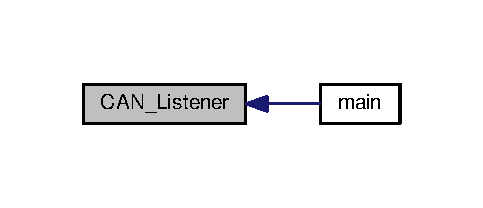
\includegraphics[width=232pt]{_lab6_8c_a43617af71ca5f26b8d87c7460ee110f4_icgraph}
\end{center}
\end{figure}


\hypertarget{_lab6_8c_a8df88b108bf75863b97b46c603310d3c}{\index{Lab6.\-c@{Lab6.\-c}!Controller@{Controller}}
\index{Controller@{Controller}!Lab6.c@{Lab6.\-c}}
\subsubsection[{Controller}]{\setlength{\rightskip}{0pt plus 5cm}void Controller (
\begin{DoxyParamCaption}
\item[{void}]{}
\end{DoxyParamCaption}
)}}\label{_lab6_8c_a8df88b108bf75863b97b46c603310d3c}


Definition at line 573 of file Lab6.\-c.


\begin{DoxyCode}
573                      \{
574     \textcolor{keywordflow}{while}(1)\{
575         
576         \textcolor{keywordflow}{if} (OS\_GetUsTime() >= 110000000) \{
577             motorMovement(\hyperlink{_p_w_m_dual_test_8c_aa187ea0bbd0d7736185b722178189816}{LEFTMOTOR}, \hyperlink{_p_w_m_dual_test_8c_ae19b6bb2940d2fbe0a79852b070eeafd}{STOP}, \hyperlink{_p_w_m_dual_test_8c_a00548cec6d104932bf79a65bac1c47e8}{REVERSE}, 200);
578             motorMovement(\hyperlink{_p_w_m_dual_test_8c_a76ff1c11b4defec11ea4a37cec53af8b}{RIGHTMOTOR}, \hyperlink{_p_w_m_dual_test_8c_ae19b6bb2940d2fbe0a79852b070eeafd}{STOP}, \hyperlink{_p_w_m_dual_test_8c_a00548cec6d104932bf79a65bac1c47e8}{REVERSE}, 200);
579             OS\_Kill();
580         \}
581         \textcolor{keywordflow}{if}((\hyperlink{_lab6_8c_adcea3401f53cc2d69e4f667b19e6c196}{IR1Val} > \hyperlink{_lab6_8c_a2106b37bdba5fd8fa85a477f5a6cd219}{supercloseFront} + 200) || (\hyperlink{_lab6_8c_a2b37f85b4e04e07d733d0925cafeea88}{IR2Val} > (
      \hyperlink{_lab6_8c_a70daf00b3818ebf7fd37f21c95e9def4}{supercloseRight} + 200)) || (\hyperlink{_lab6_8c_a6af4ef6e3413367b368acb7b5ba47d17}{IR3Val} > (\hyperlink{_lab6_8c_ab61536514678e958524efe11a63b19c7}{supercloseLeft} + 200)))
582         \{
583             motorMovement(\hyperlink{_p_w_m_dual_test_8c_aa187ea0bbd0d7736185b722178189816}{LEFTMOTOR}, \hyperlink{_p_w_m_dual_test_8c_a2acdc4aa0f128c9b2788707db3e6935e}{MOVE}, \hyperlink{_p_w_m_dual_test_8c_a00548cec6d104932bf79a65bac1c47e8}{REVERSE}, 200);
584             motorMovement(\hyperlink{_p_w_m_dual_test_8c_a76ff1c11b4defec11ea4a37cec53af8b}{RIGHTMOTOR}, \hyperlink{_p_w_m_dual_test_8c_a2acdc4aa0f128c9b2788707db3e6935e}{MOVE}, \hyperlink{_p_w_m_dual_test_8c_a00548cec6d104932bf79a65bac1c47e8}{REVERSE}, 200);
585 \textcolor{comment}{//            LEDS = GREEN + RED;}
586             OS\_Sleep(1);
587             \textcolor{keywordflow}{continue};
588         \}
589         
590         \textcolor{comment}{//********************* }
591         \textcolor{comment}{//compare the sides and assign size Values}
592         \textcolor{comment}{//run all three in parallel, since mutually exclusive }
593         
594         \textcolor{comment}{//rightWheele closer }
595         \textcolor{keywordflow}{if}(\hyperlink{_lab6_8c_a2b37f85b4e04e07d733d0925cafeea88}{IR2Val} > \hyperlink{_lab6_8c_a6af4ef6e3413367b368acb7b5ba47d17}{IR3Val})\{
596             \hyperlink{_lab6_8c_af345627334acfcd100f4da69040d289f}{longSideIRValue} = \hyperlink{_lab6_8c_a6af4ef6e3413367b368acb7b5ba47d17}{IR3Val};
597             \hyperlink{_lab6_8c_a1a6f4bd929a31fce794281d3a5fece6f}{shortSideIRValue} = \hyperlink{_lab6_8c_a2b37f85b4e04e07d733d0925cafeea88}{IR2Val};
598             \hyperlink{_lab6_8c_a32dba967fa49fbed99ed3c9531b3c3c4}{turnLeft} = 1; 
599             \hyperlink{_lab6_8c_adc8b36b959ce03ee202b7b33bb71655d}{turnRight} = 0; 
600             \hyperlink{_lab6_8c_ac17b395804882db11d8bd30dd0d5c9be}{goStraight} = 0; 
601             \hyperlink{_lab6_8c_a0e75101dc7809e2492fe0f8daed22f0a}{rightError} = 1.0 - ((float)\hyperlink{_lab6_8c_af345627334acfcd100f4da69040d289f}{longSideIRValue})/((float)
      \hyperlink{_lab6_8c_a1a6f4bd929a31fce794281d3a5fece6f}{shortSideIRValue});
602             \hyperlink{_lab6_8c_a8bbf6a7278a0b02cbd90723dc8f19bbe}{leftError} =  ((float)\hyperlink{_lab6_8c_af345627334acfcd100f4da69040d289f}{longSideIRValue})/((float)shortSideIRValue) - 1.0;
603         \}
604         \textcolor{comment}{//left Wheele closer }
605         \textcolor{keywordflow}{if}(\hyperlink{_lab6_8c_a6af4ef6e3413367b368acb7b5ba47d17}{IR3Val} > \hyperlink{_lab6_8c_a2b37f85b4e04e07d733d0925cafeea88}{IR2Val})\{
606             \hyperlink{_lab6_8c_af345627334acfcd100f4da69040d289f}{longSideIRValue} = \hyperlink{_lab6_8c_a2b37f85b4e04e07d733d0925cafeea88}{IR2Val};
607             \hyperlink{_lab6_8c_a1a6f4bd929a31fce794281d3a5fece6f}{shortSideIRValue} = \hyperlink{_lab6_8c_a6af4ef6e3413367b368acb7b5ba47d17}{IR3Val};
608             \hyperlink{_lab6_8c_a32dba967fa49fbed99ed3c9531b3c3c4}{turnLeft} = 0; 
609             \hyperlink{_lab6_8c_adc8b36b959ce03ee202b7b33bb71655d}{turnRight} = 1; 
610             \hyperlink{_lab6_8c_ac17b395804882db11d8bd30dd0d5c9be}{goStraight} = 0; 
611             \hyperlink{_lab6_8c_a8bbf6a7278a0b02cbd90723dc8f19bbe}{leftError} = 1.0 - ((float)\hyperlink{_lab6_8c_af345627334acfcd100f4da69040d289f}{longSideIRValue})/((float)
      \hyperlink{_lab6_8c_a1a6f4bd929a31fce794281d3a5fece6f}{shortSideIRValue});
612             \hyperlink{_lab6_8c_a0e75101dc7809e2492fe0f8daed22f0a}{rightError} =  ((float)\hyperlink{_lab6_8c_af345627334acfcd100f4da69040d289f}{longSideIRValue})/((float)shortSideIRValue) - 1.0
      ;
613         \}
614         \textcolor{comment}{//equal distance }
615         \textcolor{keywordflow}{if}(\hyperlink{_lab6_8c_a6af4ef6e3413367b368acb7b5ba47d17}{IR3Val} == \hyperlink{_lab6_8c_a2b37f85b4e04e07d733d0925cafeea88}{IR2Val})\{
616             \hyperlink{_lab6_8c_a0e75101dc7809e2492fe0f8daed22f0a}{rightError} = 0; 
617             \hyperlink{_lab6_8c_a8bbf6a7278a0b02cbd90723dc8f19bbe}{leftError} = 0; 
618             \hyperlink{_lab6_8c_af345627334acfcd100f4da69040d289f}{longSideIRValue} = \hyperlink{_lab6_8c_a2b37f85b4e04e07d733d0925cafeea88}{IR2Val};
619             \hyperlink{_lab6_8c_a1a6f4bd929a31fce794281d3a5fece6f}{shortSideIRValue} = \hyperlink{_lab6_8c_a6af4ef6e3413367b368acb7b5ba47d17}{IR3Val};
620             \hyperlink{_lab6_8c_a32dba967fa49fbed99ed3c9531b3c3c4}{turnLeft} = 0; 
621             \hyperlink{_lab6_8c_adc8b36b959ce03ee202b7b33bb71655d}{turnRight} = 0; 
622             \hyperlink{_lab6_8c_ac17b395804882db11d8bd30dd0d5c9be}{goStraight} = 1; 
623         \}
624          
625         \hyperlink{_lab6_8c_aca879141a9e2660e4cd8e410208fc1ec}{frontError} = (((float)\hyperlink{_lab6_8c_adcea3401f53cc2d69e4f667b19e6c196}{IR1Val} - \hyperlink{_lab6_8c_a3a69578ffb800441a624e2411824678a}{frontThreashold})/ (float)
      \hyperlink{_lab6_8c_a82059da765869f30361bcd1248568240}{tooCloseThreadshold});
626        
627         \textcolor{comment}{//}
628         \textcolor{comment}{//is front too close}
629         \textcolor{keywordflow}{if}(\hyperlink{_lab6_8c_adcea3401f53cc2d69e4f667b19e6c196}{IR1Val} >= \hyperlink{_lab6_8c_a3a69578ffb800441a624e2411824678a}{frontThreashold})\{
630             \hyperlink{_lab6_8c_ac3ef240984425a8e29bb603088b9a869}{tooCloseInFront} = 1;
631             \textcolor{comment}{//LEDS = RED;}
632         \}\textcolor{keywordflow}{else}\{
633             \hyperlink{_lab6_8c_ac3ef240984425a8e29bb603088b9a869}{tooCloseInFront} = 0;
634         \}
635         
636         \textcolor{keywordflow}{if}(\hyperlink{_lab6_8c_a2b37f85b4e04e07d733d0925cafeea88}{IR2Val} >= \hyperlink{_lab6_8c_a963dbd4c4a8ee1db8f2be5fbf95b9cd7}{rightThreashold} + 
      \hyperlink{_lab6_8c_ac62b880f4d9f55e7955e5865274708be}{tooCloseInRightCounter})\{
637             \hyperlink{_lab6_8c_a69f912c5367b8513e06ce33f7aa4b503}{tooCloseInRight} = 1;
638         \}\textcolor{keywordflow}{else}\{
639             \hyperlink{_lab6_8c_ac62b880f4d9f55e7955e5865274708be}{tooCloseInRightCounter} = 0;
640             \hyperlink{_lab6_8c_a69f912c5367b8513e06ce33f7aa4b503}{tooCloseInRight} = 0;
641         \}
642         
643         
644         \textcolor{keywordflow}{if}(\hyperlink{_lab6_8c_a6af4ef6e3413367b368acb7b5ba47d17}{IR3Val} >= \hyperlink{_lab6_8c_ac78d4fe1eb5883199c0cb9fe89ff3d8c}{leftThreashold} + \hyperlink{_lab6_8c_aea00d2299c013839953781c31d79a483}{tooCloseInLeftCounter})\{
645             \hyperlink{_lab6_8c_a6e7a0545c47884fe18d22fef9853eedb}{tooCloseInLeft} = 1;
646         \}\textcolor{keywordflow}{else}\{
647             \hyperlink{_lab6_8c_aea00d2299c013839953781c31d79a483}{tooCloseInLeftCounter} = 0;
648             \hyperlink{_lab6_8c_a6e7a0545c47884fe18d22fef9853eedb}{tooCloseInLeft} = 0;
649         \}
650         
651         
652 
653         \textcolor{comment}{//setting up the P }
654         \textcolor{comment}{// P = (shortSideIRValue - longSideIRValue)/ (shortSideIRValue + longSideIRValue);}
655         \hyperlink{_lab6_8c_aca74a684c7823144d7962beb8397621e}{P} = ((float)\hyperlink{_lab6_8c_af345627334acfcd100f4da69040d289f}{longSideIRValue})/ ((float)\hyperlink{_lab6_8c_a1a6f4bd929a31fce794281d3a5fece6f}{shortSideIRValue} );
656         
657         \textcolor{comment}{//setting up the  I}
658         \hyperlink{_lab6_8c_ae141a7ed52ba64f2053069a723a6b1fb}{leftCorrection} =  \hyperlink{_lab6_8c_ae141a7ed52ba64f2053069a723a6b1fb}{leftCorrection} + \hyperlink{_lab6_8c_aa7d5dd64817c03d067d0e922cd35d75c}{KI} * 
      \hyperlink{_lab6_8c_a8bbf6a7278a0b02cbd90723dc8f19bbe}{leftError}; 
659         \hyperlink{_lab6_8c_ae156e47c164a3c02c27a3117ce45696c}{rightCorrection} =  \hyperlink{_lab6_8c_ae156e47c164a3c02c27a3117ce45696c}{rightCorrection} + \hyperlink{_lab6_8c_aa7d5dd64817c03d067d0e922cd35d75c}{KI} * 
      \hyperlink{_lab6_8c_a0e75101dc7809e2492fe0f8daed22f0a}{rightError}; 
660         \textcolor{comment}{//capping corrections}
661         \textcolor{keywordflow}{if} (\hyperlink{_lab6_8c_ae141a7ed52ba64f2053069a723a6b1fb}{leftCorrection} > \hyperlink{_lab6_8c_ab639d295e81c2bcff1a343f7cc1273f7}{highCorrectionCap}) 
662             \hyperlink{_lab6_8c_ae141a7ed52ba64f2053069a723a6b1fb}{leftCorrection} = \hyperlink{_lab6_8c_ab639d295e81c2bcff1a343f7cc1273f7}{highCorrectionCap}; 
663         \textcolor{keywordflow}{else} \textcolor{keywordflow}{if} ( \hyperlink{_lab6_8c_ae141a7ed52ba64f2053069a723a6b1fb}{leftCorrection} < \hyperlink{_lab6_8c_ad567eeac9df9c00f413fb04eecc4d68b}{lowCorrectionCap}) 
664             \hyperlink{_lab6_8c_ae141a7ed52ba64f2053069a723a6b1fb}{leftCorrection} = \hyperlink{_lab6_8c_ad567eeac9df9c00f413fb04eecc4d68b}{lowCorrectionCap}; 
665 
666         \textcolor{keywordflow}{if} (\hyperlink{_lab6_8c_ae156e47c164a3c02c27a3117ce45696c}{rightCorrection} > \hyperlink{_lab6_8c_ab639d295e81c2bcff1a343f7cc1273f7}{highCorrectionCap}) 
667             \hyperlink{_lab6_8c_ae156e47c164a3c02c27a3117ce45696c}{rightCorrection} = \hyperlink{_lab6_8c_ab639d295e81c2bcff1a343f7cc1273f7}{highCorrectionCap}; 
668         \textcolor{keywordflow}{else} \textcolor{keywordflow}{if} ( \hyperlink{_lab6_8c_ae156e47c164a3c02c27a3117ce45696c}{rightCorrection} < \hyperlink{_lab6_8c_ad567eeac9df9c00f413fb04eecc4d68b}{lowCorrectionCap}) 
669             \hyperlink{_lab6_8c_ae156e47c164a3c02c27a3117ce45696c}{rightCorrection} = \hyperlink{_lab6_8c_ad567eeac9df9c00f413fb04eecc4d68b}{lowCorrectionCap}; 
670 
671         
672         \textcolor{comment}{//navigate based on the sensor inputs so far}
673         \textcolor{comment}{//run all three in paralell, since mutually exclusive }
674         \textcolor{comment}{//set the motorSpeed }
675         \textcolor{keywordflow}{if} (\hyperlink{_lab6_8c_a32dba967fa49fbed99ed3c9531b3c3c4}{turnLeft}) \{
676             \hyperlink{_lab6_8c_a61686d33603491344883775b9b31e172}{LEDS} = \hyperlink{_lab6_8c_acfbc006ea433ad708fdee3e82996e721}{GREEN}; 
677             \hyperlink{_lab6_8c_ac2c5dad90c7edb32a33bf01d49ddfddb}{rightMotorSpeed} = \hyperlink{_lab6_8c_a050ff1c0feff586146c87aeac96fdbe2}{highestSpeed};  \textcolor{comment}{//might be set to highestSpeed or
       Higher}
678             \textcolor{keywordflow}{if} (\hyperlink{_lab6_8c_aca74a684c7823144d7962beb8397621e}{P} > 1 )\{ \textcolor{comment}{//regulate if multipliaction caps out}
679                 \hyperlink{_lab6_8c_ace43f08f7bad6f10c2df24b2df25f6bb}{leftMotorSpeed} = \hyperlink{_lab6_8c_a050ff1c0feff586146c87aeac96fdbe2}{highestSpeed} - 40;
680                 \hyperlink{_lab6_8c_a61686d33603491344883775b9b31e172}{LEDS} = \hyperlink{_lab6_8c_a87b537f5fa5c109d3c05c13d6b18f382}{WHITE};
681             \}\textcolor{keywordflow}{else}\{
682                 \hyperlink{_lab6_8c_ace43f08f7bad6f10c2df24b2df25f6bb}{leftMotorSpeed} = \hyperlink{_lab6_8c_a050ff1c0feff586146c87aeac96fdbe2}{highestSpeed}*(\hyperlink{_lab6_8c_aca74a684c7823144d7962beb8397621e}{P}) + 
      \hyperlink{_lab6_8c_ae156e47c164a3c02c27a3117ce45696c}{rightCorrection};
683             \}
684             
685             \textcolor{comment}{//capping the speed }
686             \textcolor{keywordflow}{if}(\hyperlink{_lab6_8c_ace43f08f7bad6f10c2df24b2df25f6bb}{leftMotorSpeed} > \hyperlink{_lab6_8c_a050ff1c0feff586146c87aeac96fdbe2}{highestSpeed})\{ 
687                 \hyperlink{_lab6_8c_ace43f08f7bad6f10c2df24b2df25f6bb}{leftMotorSpeed}  = \hyperlink{_lab6_8c_a050ff1c0feff586146c87aeac96fdbe2}{highestSpeed}; 
688                 \hyperlink{_lab6_8c_a61686d33603491344883775b9b31e172}{LEDS} = \hyperlink{_lab6_8c_a87b537f5fa5c109d3c05c13d6b18f382}{WHITE};
689             \} \textcolor{keywordflow}{else} \textcolor{keywordflow}{if} (\hyperlink{_lab6_8c_ace43f08f7bad6f10c2df24b2df25f6bb}{leftMotorSpeed} < \hyperlink{_lab6_8c_a2ea64ff9e3f348639493e6ec84013d98}{lowestSpeed}) \{
690                 \hyperlink{_lab6_8c_a61686d33603491344883775b9b31e172}{LEDS} = \hyperlink{_lab6_8c_a87b537f5fa5c109d3c05c13d6b18f382}{WHITE};
691                 \hyperlink{_lab6_8c_ace43f08f7bad6f10c2df24b2df25f6bb}{leftMotorSpeed}  = \hyperlink{_lab6_8c_a2ea64ff9e3f348639493e6ec84013d98}{lowestSpeed}; 
692             \}
693         \}
694         \textcolor{keywordflow}{if} (\hyperlink{_lab6_8c_adc8b36b959ce03ee202b7b33bb71655d}{turnRight}) \{
695             \hyperlink{_lab6_8c_a61686d33603491344883775b9b31e172}{LEDS} = \hyperlink{_lab6_8c_a79d10e672abb49ad63eeaa8aaef57c38}{BLUE}; 
696             \hyperlink{_lab6_8c_ace43f08f7bad6f10c2df24b2df25f6bb}{leftMotorSpeed} = \hyperlink{_lab6_8c_a050ff1c0feff586146c87aeac96fdbe2}{highestSpeed};  \textcolor{comment}{//might be set to highestSpeed or
       Higher}
697             \textcolor{keywordflow}{if} (\hyperlink{_lab6_8c_aca74a684c7823144d7962beb8397621e}{P} > 1 )\{ \textcolor{comment}{//if this multiplication causes maxing out the speedg}
698                 \hyperlink{_lab6_8c_ac2c5dad90c7edb32a33bf01d49ddfddb}{rightMotorSpeed} = \hyperlink{_lab6_8c_a050ff1c0feff586146c87aeac96fdbe2}{highestSpeed} - 40;
699             \}\textcolor{keywordflow}{else}\{
700                 \hyperlink{_lab6_8c_ac2c5dad90c7edb32a33bf01d49ddfddb}{rightMotorSpeed} = \hyperlink{_lab6_8c_a050ff1c0feff586146c87aeac96fdbe2}{highestSpeed}*(\hyperlink{_lab6_8c_aca74a684c7823144d7962beb8397621e}{P}) + 
      \hyperlink{_lab6_8c_ae141a7ed52ba64f2053069a723a6b1fb}{leftCorrection};
701             \}
702 
703             \textcolor{comment}{//capping the speed }
704             \textcolor{keywordflow}{if}(\hyperlink{_lab6_8c_ac2c5dad90c7edb32a33bf01d49ddfddb}{rightMotorSpeed} > \hyperlink{_lab6_8c_a050ff1c0feff586146c87aeac96fdbe2}{highestSpeed})\{ 
705                 \hyperlink{_lab6_8c_ac2c5dad90c7edb32a33bf01d49ddfddb}{rightMotorSpeed}  = \hyperlink{_lab6_8c_a050ff1c0feff586146c87aeac96fdbe2}{highestSpeed}; 
706                 \hyperlink{_lab6_8c_a61686d33603491344883775b9b31e172}{LEDS} = \hyperlink{_lab6_8c_a87b537f5fa5c109d3c05c13d6b18f382}{WHITE};
707             \}  \textcolor{keywordflow}{else} \textcolor{keywordflow}{if} (\hyperlink{_lab6_8c_ac2c5dad90c7edb32a33bf01d49ddfddb}{rightMotorSpeed} < \hyperlink{_lab6_8c_a2ea64ff9e3f348639493e6ec84013d98}{lowestSpeed}) \{
708                 \hyperlink{_lab6_8c_ac2c5dad90c7edb32a33bf01d49ddfddb}{rightMotorSpeed}  = \hyperlink{_lab6_8c_a2ea64ff9e3f348639493e6ec84013d98}{lowestSpeed}; 
709             \}
710 
711         \}
712         
713         \textcolor{keywordflow}{if}  (\hyperlink{_lab6_8c_ac17b395804882db11d8bd30dd0d5c9be}{goStraight}) \{
714             \hyperlink{_lab6_8c_ace43f08f7bad6f10c2df24b2df25f6bb}{leftMotorSpeed} = \hyperlink{_lab6_8c_a050ff1c0feff586146c87aeac96fdbe2}{highestSpeed};  \textcolor{comment}{//might be set to highestSpeed or
       Higher}
715             \hyperlink{_lab6_8c_ac2c5dad90c7edb32a33bf01d49ddfddb}{rightMotorSpeed} = \hyperlink{_lab6_8c_a050ff1c0feff586146c87aeac96fdbe2}{highestSpeed} ;
716         \}
717 
718         \textcolor{comment}{//run the Motors }
719         \textcolor{comment}{//if too close, stop one wheele}
720         \textcolor{keywordflow}{if}(\hyperlink{_lab6_8c_ac3ef240984425a8e29bb603088b9a869}{tooCloseInFront} == 1) \{ 
721             \hyperlink{_lab6_8c_a61686d33603491344883775b9b31e172}{LEDS} = \hyperlink{_lab6_8c_a8d23feea868a983c8c2b661e1e16972f}{RED}; 
722             \textcolor{keywordflow}{if}(\hyperlink{_lab6_8c_adc8b36b959ce03ee202b7b33bb71655d}{turnRight}) \{
723                 \hyperlink{_lab6_8c_ace43f08f7bad6f10c2df24b2df25f6bb}{leftMotorSpeed} = \hyperlink{_lab6_8c_a08f684c971e5e14bcd9ded712ffc8e31}{frontHighestSpeed}; 
724                 \hyperlink{_lab6_8c_ac2c5dad90c7edb32a33bf01d49ddfddb}{rightMotorSpeed} = 60*(1.0 - \hyperlink{_lab6_8c_aca879141a9e2660e4cd8e410208fc1ec}{frontError}); 
725                 \textcolor{keywordflow}{if} (\hyperlink{_lab6_8c_ac2c5dad90c7edb32a33bf01d49ddfddb}{rightMotorSpeed} < \hyperlink{_lab6_8c_a4e5311a153c7dc8b2e6160e3733ddb4d}{frontLowCap}) \{
726                     \hyperlink{_lab6_8c_a61686d33603491344883775b9b31e172}{LEDS}= \hyperlink{_lab6_8c_a87b537f5fa5c109d3c05c13d6b18f382}{WHITE}; 
727                     \textcolor{comment}{//rightMotorSpeed = 0;}
728                     motorMovement(\hyperlink{_p_w_m_dual_test_8c_aa187ea0bbd0d7736185b722178189816}{LEFTMOTOR}, \hyperlink{_p_w_m_dual_test_8c_a2acdc4aa0f128c9b2788707db3e6935e}{MOVE}, \hyperlink{_p_w_m_dual_test_8c_a6ddfdda7a062d10cff4a72b76b44aeb8}{FORWARD},
      \hyperlink{_lab6_8c_ace43f08f7bad6f10c2df24b2df25f6bb}{leftMotorSpeed});
729                     motorMovement(\hyperlink{_p_w_m_dual_test_8c_a76ff1c11b4defec11ea4a37cec53af8b}{RIGHTMOTOR}, \hyperlink{_p_w_m_dual_test_8c_ae19b6bb2940d2fbe0a79852b070eeafd}{STOP}, \hyperlink{_p_w_m_dual_test_8c_a6ddfdda7a062d10cff4a72b76b44aeb8}{FORWARD},
      \hyperlink{_lab6_8c_ac2c5dad90c7edb32a33bf01d49ddfddb}{rightMotorSpeed});
730                 \}\textcolor{keywordflow}{else} \{
731                     motorMovement(\hyperlink{_p_w_m_dual_test_8c_a76ff1c11b4defec11ea4a37cec53af8b}{RIGHTMOTOR}, \hyperlink{_p_w_m_dual_test_8c_a2acdc4aa0f128c9b2788707db3e6935e}{MOVE}, \hyperlink{_p_w_m_dual_test_8c_a6ddfdda7a062d10cff4a72b76b44aeb8}{FORWARD},
      \hyperlink{_lab6_8c_ac2c5dad90c7edb32a33bf01d49ddfddb}{rightMotorSpeed});
732                     motorMovement(\hyperlink{_p_w_m_dual_test_8c_aa187ea0bbd0d7736185b722178189816}{LEFTMOTOR}, \hyperlink{_p_w_m_dual_test_8c_a2acdc4aa0f128c9b2788707db3e6935e}{MOVE}, \hyperlink{_p_w_m_dual_test_8c_a6ddfdda7a062d10cff4a72b76b44aeb8}{FORWARD},
      \hyperlink{_lab6_8c_ace43f08f7bad6f10c2df24b2df25f6bb}{leftMotorSpeed});
733                 \}
734                 \textcolor{comment}{//rightMotorSpeed = 1/ }
735                 \textcolor{comment}{//motorMovement(RIGHTMOTOR, STOP, FORWARD,rightMotorSpeed);}
736             \}
737             \textcolor{keywordflow}{if}(\hyperlink{_lab6_8c_a32dba967fa49fbed99ed3c9531b3c3c4}{turnLeft}) \{
738                 \textcolor{comment}{//motorMovement(LEFTMOTOR, STOP, FORWARD,leftMotorSpeed);}
739                 \hyperlink{_lab6_8c_ac2c5dad90c7edb32a33bf01d49ddfddb}{rightMotorSpeed} = \hyperlink{_lab6_8c_a08f684c971e5e14bcd9ded712ffc8e31}{frontHighestSpeed}; 
740                 \hyperlink{_lab6_8c_ace43f08f7bad6f10c2df24b2df25f6bb}{leftMotorSpeed} = 60*(1.0 - \hyperlink{_lab6_8c_aca879141a9e2660e4cd8e410208fc1ec}{frontError}); 
741                 \textcolor{keywordflow}{if} (\hyperlink{_lab6_8c_ace43f08f7bad6f10c2df24b2df25f6bb}{leftMotorSpeed} < \hyperlink{_lab6_8c_a4e5311a153c7dc8b2e6160e3733ddb4d}{frontLowCap}) \{
742                     \hyperlink{_lab6_8c_a61686d33603491344883775b9b31e172}{LEDS}= \hyperlink{_lab6_8c_a87b537f5fa5c109d3c05c13d6b18f382}{WHITE}; 
743                     \textcolor{comment}{//leftMotorSpeed = 0;}
744                     motorMovement(\hyperlink{_p_w_m_dual_test_8c_aa187ea0bbd0d7736185b722178189816}{LEFTMOTOR}, \hyperlink{_p_w_m_dual_test_8c_ae19b6bb2940d2fbe0a79852b070eeafd}{STOP}, \hyperlink{_p_w_m_dual_test_8c_a6ddfdda7a062d10cff4a72b76b44aeb8}{FORWARD},
      \hyperlink{_lab6_8c_ace43f08f7bad6f10c2df24b2df25f6bb}{leftMotorSpeed});
745                     motorMovement(\hyperlink{_p_w_m_dual_test_8c_a76ff1c11b4defec11ea4a37cec53af8b}{RIGHTMOTOR}, \hyperlink{_p_w_m_dual_test_8c_a2acdc4aa0f128c9b2788707db3e6935e}{MOVE}, \hyperlink{_p_w_m_dual_test_8c_a6ddfdda7a062d10cff4a72b76b44aeb8}{FORWARD},
      \hyperlink{_lab6_8c_ac2c5dad90c7edb32a33bf01d49ddfddb}{rightMotorSpeed});
746                 \}\textcolor{keywordflow}{else} \{
747                     motorMovement(\hyperlink{_p_w_m_dual_test_8c_a76ff1c11b4defec11ea4a37cec53af8b}{RIGHTMOTOR}, \hyperlink{_p_w_m_dual_test_8c_a2acdc4aa0f128c9b2788707db3e6935e}{MOVE}, \hyperlink{_p_w_m_dual_test_8c_a6ddfdda7a062d10cff4a72b76b44aeb8}{FORWARD},
      \hyperlink{_lab6_8c_ac2c5dad90c7edb32a33bf01d49ddfddb}{rightMotorSpeed});
748                     motorMovement(\hyperlink{_p_w_m_dual_test_8c_aa187ea0bbd0d7736185b722178189816}{LEFTMOTOR}, \hyperlink{_p_w_m_dual_test_8c_a2acdc4aa0f128c9b2788707db3e6935e}{MOVE}, \hyperlink{_p_w_m_dual_test_8c_a6ddfdda7a062d10cff4a72b76b44aeb8}{FORWARD},
      \hyperlink{_lab6_8c_ace43f08f7bad6f10c2df24b2df25f6bb}{leftMotorSpeed});
749                 \}
750             \}
751         \} \textcolor{keywordflow}{else} \textcolor{keywordflow}{if} (\hyperlink{_lab6_8c_a69f912c5367b8513e06ce33f7aa4b503}{tooCloseInRight}  == 1)\{
752             \hyperlink{_lab6_8c_ac62b880f4d9f55e7955e5865274708be}{tooCloseInRightCounter} +=30; 
753             \hyperlink{_lab6_8c_ac2c5dad90c7edb32a33bf01d49ddfddb}{rightMotorSpeed} = \hyperlink{_lab6_8c_a4e956e2d600928dfbbe5b2440c53a223}{sideHighestSpeed}; 
754             \hyperlink{_lab6_8c_ace43f08f7bad6f10c2df24b2df25f6bb}{leftMotorSpeed} = 210*(1.0 - \hyperlink{_lab6_8c_a0e75101dc7809e2492fe0f8daed22f0a}{rightError}); 
755             \textcolor{keywordflow}{if} (\hyperlink{_lab6_8c_ace43f08f7bad6f10c2df24b2df25f6bb}{leftMotorSpeed} < 150) \{
756                 \textcolor{comment}{//leftMotorSpeed = 0;}
757                 \hyperlink{_lab6_8c_a61686d33603491344883775b9b31e172}{LEDS}= \hyperlink{_lab6_8c_a87b537f5fa5c109d3c05c13d6b18f382}{WHITE}; 
758                 motorMovement(\hyperlink{_p_w_m_dual_test_8c_aa187ea0bbd0d7736185b722178189816}{LEFTMOTOR}, \hyperlink{_p_w_m_dual_test_8c_a2acdc4aa0f128c9b2788707db3e6935e}{MOVE}, \hyperlink{_p_w_m_dual_test_8c_a6ddfdda7a062d10cff4a72b76b44aeb8}{FORWARD},150);
759                 motorMovement(\hyperlink{_p_w_m_dual_test_8c_a76ff1c11b4defec11ea4a37cec53af8b}{RIGHTMOTOR}, \hyperlink{_p_w_m_dual_test_8c_a2acdc4aa0f128c9b2788707db3e6935e}{MOVE}, \hyperlink{_p_w_m_dual_test_8c_a6ddfdda7a062d10cff4a72b76b44aeb8}{FORWARD},
      \hyperlink{_lab6_8c_ac2c5dad90c7edb32a33bf01d49ddfddb}{rightMotorSpeed});
760             \}\textcolor{keywordflow}{else} \{
761                 motorMovement(\hyperlink{_p_w_m_dual_test_8c_a76ff1c11b4defec11ea4a37cec53af8b}{RIGHTMOTOR}, \hyperlink{_p_w_m_dual_test_8c_a2acdc4aa0f128c9b2788707db3e6935e}{MOVE}, \hyperlink{_p_w_m_dual_test_8c_a6ddfdda7a062d10cff4a72b76b44aeb8}{FORWARD},
      \hyperlink{_lab6_8c_ac2c5dad90c7edb32a33bf01d49ddfddb}{rightMotorSpeed});
762                 motorMovement(\hyperlink{_p_w_m_dual_test_8c_aa187ea0bbd0d7736185b722178189816}{LEFTMOTOR}, \hyperlink{_p_w_m_dual_test_8c_a2acdc4aa0f128c9b2788707db3e6935e}{MOVE}, \hyperlink{_p_w_m_dual_test_8c_a6ddfdda7a062d10cff4a72b76b44aeb8}{FORWARD},
      \hyperlink{_lab6_8c_ace43f08f7bad6f10c2df24b2df25f6bb}{leftMotorSpeed});
763                 \hyperlink{_lab6_8c_a61686d33603491344883775b9b31e172}{LEDS} = \hyperlink{_lab6_8c_a8d23feea868a983c8c2b661e1e16972f}{RED} + \hyperlink{_lab6_8c_a79d10e672abb49ad63eeaa8aaef57c38}{BLUE};
764             \}
765         \} \textcolor{keywordflow}{else} \textcolor{keywordflow}{if} (\hyperlink{_lab6_8c_a6e7a0545c47884fe18d22fef9853eedb}{tooCloseInLeft}  == 1)\{
766             \hyperlink{_lab6_8c_aea00d2299c013839953781c31d79a483}{tooCloseInLeftCounter} +=30; 
767             \hyperlink{_lab6_8c_ace43f08f7bad6f10c2df24b2df25f6bb}{leftMotorSpeed} = \hyperlink{_lab6_8c_a4e956e2d600928dfbbe5b2440c53a223}{sideHighestSpeed}; 
768             \hyperlink{_lab6_8c_ac2c5dad90c7edb32a33bf01d49ddfddb}{rightMotorSpeed} = 210*(1.0 - \hyperlink{_lab6_8c_a8bbf6a7278a0b02cbd90723dc8f19bbe}{leftError}); 
769             \textcolor{keywordflow}{if} (\hyperlink{_lab6_8c_ac2c5dad90c7edb32a33bf01d49ddfddb}{rightMotorSpeed} < 150) \{
770                 \hyperlink{_lab6_8c_a61686d33603491344883775b9b31e172}{LEDS}= \hyperlink{_lab6_8c_a87b537f5fa5c109d3c05c13d6b18f382}{WHITE}; 
771                 \textcolor{comment}{//leftMotorSpeed = 0;}
772                 motorMovement(\hyperlink{_p_w_m_dual_test_8c_aa187ea0bbd0d7736185b722178189816}{LEFTMOTOR}, \hyperlink{_p_w_m_dual_test_8c_a2acdc4aa0f128c9b2788707db3e6935e}{MOVE}, \hyperlink{_p_w_m_dual_test_8c_a6ddfdda7a062d10cff4a72b76b44aeb8}{FORWARD},
      \hyperlink{_lab6_8c_ace43f08f7bad6f10c2df24b2df25f6bb}{leftMotorSpeed});
773                 motorMovement(\hyperlink{_p_w_m_dual_test_8c_a76ff1c11b4defec11ea4a37cec53af8b}{RIGHTMOTOR},\hyperlink{_p_w_m_dual_test_8c_a2acdc4aa0f128c9b2788707db3e6935e}{MOVE}, \hyperlink{_p_w_m_dual_test_8c_a6ddfdda7a062d10cff4a72b76b44aeb8}{FORWARD},150);
774             \}\textcolor{keywordflow}{else} \{
775                 motorMovement(\hyperlink{_p_w_m_dual_test_8c_a76ff1c11b4defec11ea4a37cec53af8b}{RIGHTMOTOR}, \hyperlink{_p_w_m_dual_test_8c_a2acdc4aa0f128c9b2788707db3e6935e}{MOVE}, \hyperlink{_p_w_m_dual_test_8c_a6ddfdda7a062d10cff4a72b76b44aeb8}{FORWARD},
      \hyperlink{_lab6_8c_ac2c5dad90c7edb32a33bf01d49ddfddb}{rightMotorSpeed});
776                 motorMovement(\hyperlink{_p_w_m_dual_test_8c_aa187ea0bbd0d7736185b722178189816}{LEFTMOTOR}, \hyperlink{_p_w_m_dual_test_8c_a2acdc4aa0f128c9b2788707db3e6935e}{MOVE}, \hyperlink{_p_w_m_dual_test_8c_a6ddfdda7a062d10cff4a72b76b44aeb8}{FORWARD},
      \hyperlink{_lab6_8c_ace43f08f7bad6f10c2df24b2df25f6bb}{leftMotorSpeed});
777                 \hyperlink{_lab6_8c_a61686d33603491344883775b9b31e172}{LEDS} = \hyperlink{_lab6_8c_a8d23feea868a983c8c2b661e1e16972f}{RED} + \hyperlink{_lab6_8c_a79d10e672abb49ad63eeaa8aaef57c38}{BLUE};
778             \}
779         \}\textcolor{keywordflow}{else}\{ 
780             motorMovement(\hyperlink{_p_w_m_dual_test_8c_aa187ea0bbd0d7736185b722178189816}{LEFTMOTOR}, \hyperlink{_p_w_m_dual_test_8c_a2acdc4aa0f128c9b2788707db3e6935e}{MOVE}, \hyperlink{_p_w_m_dual_test_8c_a6ddfdda7a062d10cff4a72b76b44aeb8}{FORWARD},
      \hyperlink{_lab6_8c_ace43f08f7bad6f10c2df24b2df25f6bb}{leftMotorSpeed});
781             motorMovement(\hyperlink{_p_w_m_dual_test_8c_a76ff1c11b4defec11ea4a37cec53af8b}{RIGHTMOTOR}, \hyperlink{_p_w_m_dual_test_8c_a2acdc4aa0f128c9b2788707db3e6935e}{MOVE}, \hyperlink{_p_w_m_dual_test_8c_a6ddfdda7a062d10cff4a72b76b44aeb8}{FORWARD},
      \hyperlink{_lab6_8c_ac2c5dad90c7edb32a33bf01d49ddfddb}{rightMotorSpeed});
782         \}
783 
784         \textcolor{comment}{//go to sleep for a while  }
785         OS\_Sleep(1);
786     \}
787     OS\_Kill();
788 \}
\end{DoxyCode}


Here is the caller graph for this function\-:
\nopagebreak
\begin{figure}[H]
\begin{center}
\leavevmode
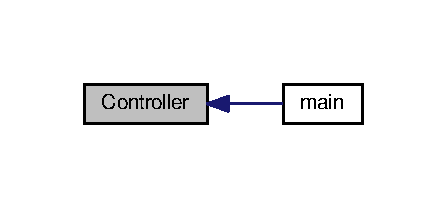
\includegraphics[width=214pt]{_lab6_8c_a8df88b108bf75863b97b46c603310d3c_icgraph}
\end{center}
\end{figure}


\hypertarget{_lab6_8c_abced8d67df156821551c29a1cb684a05}{\index{Lab6.\-c@{Lab6.\-c}!Controller2@{Controller2}}
\index{Controller2@{Controller2}!Lab6.c@{Lab6.\-c}}
\subsubsection[{Controller2}]{\setlength{\rightskip}{0pt plus 5cm}void Controller2 (
\begin{DoxyParamCaption}
\item[{void}]{}
\end{DoxyParamCaption}
)}}\label{_lab6_8c_abced8d67df156821551c29a1cb684a05}


Definition at line 559 of file Lab6.\-c.


\begin{DoxyCode}
559                       \{
560      \textcolor{keywordflow}{while}(1) \{  
561 \textcolor{comment}{//         for (int i =0; i< 100000; i++)\{}
562 \textcolor{comment}{//             LEDS = BLUE; }
563 \textcolor{comment}{//         \} }
564 \textcolor{comment}{//          for (int i =0; i< 100000; i++)\{}
565 \textcolor{comment}{//             LEDS = RED; }
566 \textcolor{comment}{//         \} }
567          motorMovement(\hyperlink{_p_w_m_dual_test_8c_aa187ea0bbd0d7736185b722178189816}{LEFTMOTOR}, \hyperlink{_p_w_m_dual_test_8c_a2acdc4aa0f128c9b2788707db3e6935e}{MOVE}, \hyperlink{_p_w_m_dual_test_8c_a6ddfdda7a062d10cff4a72b76b44aeb8}{FORWARD}, 200);
568          motorMovement(\hyperlink{_p_w_m_dual_test_8c_a76ff1c11b4defec11ea4a37cec53af8b}{RIGHTMOTOR}, \hyperlink{_p_w_m_dual_test_8c_a2acdc4aa0f128c9b2788707db3e6935e}{MOVE}, \hyperlink{_p_w_m_dual_test_8c_a6ddfdda7a062d10cff4a72b76b44aeb8}{FORWARD}, 200);
569          OS\_Sleep(1);
570    \}
571     OS\_Kill();
572 \}
\end{DoxyCode}
\hypertarget{_lab6_8c_a968e17f037bc1e2ec26307388d6d17ad}{\index{Lab6.\-c@{Lab6.\-c}!death\-Ray@{death\-Ray}}
\index{death\-Ray@{death\-Ray}!Lab6.c@{Lab6.\-c}}
\subsubsection[{death\-Ray}]{\setlength{\rightskip}{0pt plus 5cm}void death\-Ray (
\begin{DoxyParamCaption}
\item[{void}]{}
\end{DoxyParamCaption}
)}}\label{_lab6_8c_a968e17f037bc1e2ec26307388d6d17ad}


Definition at line 210 of file Lab6.\-c.


\begin{DoxyCode}
210                    \{
211   \hyperlink{_lab6_8c_a1194403dd24b90c5af73482c52ad1360}{PC7} = 0x80;
212   OS\_DelayUS(5);
213   \textcolor{comment}{//Write GPIO Pin Low}
214   \hyperlink{_lab6_8c_a1194403dd24b90c5af73482c52ad1360}{PC7} = 0x00;
215 
216 
217 \}
\end{DoxyCode}


Here is the caller graph for this function\-:
\nopagebreak
\begin{figure}[H]
\begin{center}
\leavevmode
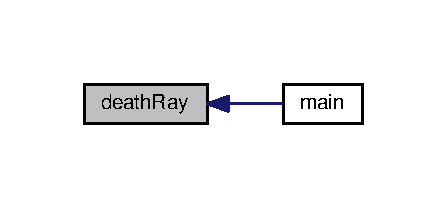
\includegraphics[width=214pt]{_lab6_8c_a968e17f037bc1e2ec26307388d6d17ad_icgraph}
\end{center}
\end{figure}


\hypertarget{_lab6_8c_ac866dbaf7b167e5c46bb33de42eee84d}{\index{Lab6.\-c@{Lab6.\-c}!Disable\-Interrupts@{Disable\-Interrupts}}
\index{Disable\-Interrupts@{Disable\-Interrupts}!Lab6.c@{Lab6.\-c}}
\subsubsection[{Disable\-Interrupts}]{\setlength{\rightskip}{0pt plus 5cm}void Disable\-Interrupts (
\begin{DoxyParamCaption}
\item[{void}]{}
\end{DoxyParamCaption}
)}}\label{_lab6_8c_ac866dbaf7b167e5c46bb33de42eee84d}
\hypertarget{_lab6_8c_ab712356331a62b04aebcb373865e68c4}{\index{Lab6.\-c@{Lab6.\-c}!Enable\-Interrupts@{Enable\-Interrupts}}
\index{Enable\-Interrupts@{Enable\-Interrupts}!Lab6.c@{Lab6.\-c}}
\subsubsection[{Enable\-Interrupts}]{\setlength{\rightskip}{0pt plus 5cm}void Enable\-Interrupts (
\begin{DoxyParamCaption}
\item[{void}]{}
\end{DoxyParamCaption}
)}}\label{_lab6_8c_ab712356331a62b04aebcb373865e68c4}
\hypertarget{_lab6_8c_a670da3ff1aea0c7d54c40e9e40b5eeed}{\index{Lab6.\-c@{Lab6.\-c}!End\-Critical@{End\-Critical}}
\index{End\-Critical@{End\-Critical}!Lab6.c@{Lab6.\-c}}
\subsubsection[{End\-Critical}]{\setlength{\rightskip}{0pt plus 5cm}void End\-Critical (
\begin{DoxyParamCaption}
\item[{long}]{sr}
\end{DoxyParamCaption}
)}}\label{_lab6_8c_a670da3ff1aea0c7d54c40e9e40b5eeed}


Here is the caller graph for this function\-:
\nopagebreak
\begin{figure}[H]
\begin{center}
\leavevmode
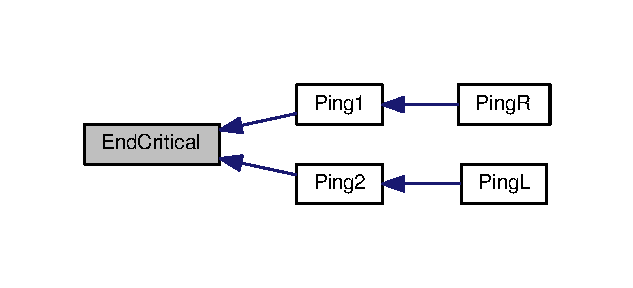
\includegraphics[width=304pt]{_lab6_8c_a670da3ff1aea0c7d54c40e9e40b5eeed_icgraph}
\end{center}
\end{figure}


\hypertarget{_lab6_8c_a6f1889c3f5d0f35d0ca0f7aa03ed5cb1}{\index{Lab6.\-c@{Lab6.\-c}!G\-P\-I\-O\-Port\-A\-\_\-\-Handler@{G\-P\-I\-O\-Port\-A\-\_\-\-Handler}}
\index{G\-P\-I\-O\-Port\-A\-\_\-\-Handler@{G\-P\-I\-O\-Port\-A\-\_\-\-Handler}!Lab6.c@{Lab6.\-c}}
\subsubsection[{G\-P\-I\-O\-Port\-A\-\_\-\-Handler}]{\setlength{\rightskip}{0pt plus 5cm}void G\-P\-I\-O\-Port\-A\-\_\-\-Handler (
\begin{DoxyParamCaption}
\item[{void}]{}
\end{DoxyParamCaption}
)}}\label{_lab6_8c_a6f1889c3f5d0f35d0ca0f7aa03ed5cb1}


Definition at line 110 of file Lab6.\-c.


\begin{DoxyCode}
110                             \{
111   GPIO\_PORTA\_ICR\_R = (1 << 6);    \textcolor{comment}{// acknowledge flag6}
112   \textcolor{comment}{//SW2 = 1;}
113   \textcolor{keyword}{static} uint32\_t pingStartTime; 
114   \textcolor{keyword}{static} uint32\_t pingEndTime;
115 
116   \textcolor{keywordflow}{if}(\hyperlink{_lab6_8c_adaab1d0c061d12c9892583c9591a70af}{PA6} != 0)  pingStartTime = OS\_GetUsTime();
117   \textcolor{keywordflow}{else} \textcolor{keywordflow}{if}(\hyperlink{_lab6_8c_adaab1d0c061d12c9892583c9591a70af}{PA6} == 0)\{
118     pingEndTime = OS\_GetUsTime();
119     uint32\_t delta =  ((pingEndTime - pingStartTime) >> 1)*34300/1000000;
120     \textcolor{keywordflow}{if}(pingEndTime > pingStartTime)\{
121       \hyperlink{_lab6_8c_a6b0304a7c2f611c97a1f4779a9bfb483}{Ping1Mail}.Send(delta);
122     \}
123   \}
124 \}
\end{DoxyCode}
\hypertarget{_lab6_8c_a0b6c07c1a985f30a5ca41d59f8c22932}{\index{Lab6.\-c@{Lab6.\-c}!G\-P\-I\-O\-Port\-C\-\_\-\-Handler@{G\-P\-I\-O\-Port\-C\-\_\-\-Handler}}
\index{G\-P\-I\-O\-Port\-C\-\_\-\-Handler@{G\-P\-I\-O\-Port\-C\-\_\-\-Handler}!Lab6.c@{Lab6.\-c}}
\subsubsection[{G\-P\-I\-O\-Port\-C\-\_\-\-Handler}]{\setlength{\rightskip}{0pt plus 5cm}void G\-P\-I\-O\-Port\-C\-\_\-\-Handler (
\begin{DoxyParamCaption}
\item[{void}]{}
\end{DoxyParamCaption}
)}}\label{_lab6_8c_a0b6c07c1a985f30a5ca41d59f8c22932}


Definition at line 125 of file Lab6.\-c.


\begin{DoxyCode}
125                             \{
126   GPIO\_PORTC\_ICR\_R = (1 << 6);    \textcolor{comment}{// acknowledge flag6}
127   \textcolor{comment}{//SW2 = 1;}
128   \textcolor{keyword}{static} uint32\_t pingStartTime; 
129   \textcolor{keyword}{static} uint32\_t pingEndTime;
130 
131   \textcolor{keywordflow}{if}(\hyperlink{_lab6_8c_aea08c09063c5962f8f60044f1829d54c}{PC6} != 0)  pingStartTime = OS\_GetUsTime();
132   \textcolor{keywordflow}{else} \textcolor{keywordflow}{if}(\hyperlink{_lab6_8c_aea08c09063c5962f8f60044f1829d54c}{PC6} == 0)\{
133     pingEndTime = OS\_GetUsTime();
134     uint32\_t delta =  ((pingEndTime - pingStartTime) >> 1)*34300/1000000;
135     \textcolor{keywordflow}{if}(pingEndTime > pingStartTime)\{
136       \hyperlink{_lab6_8c_a39dbfc1fca14892a7d8916d445fb4321}{Ping2Mail}.Send(delta);
137     \}
138   \}
139 \}
\end{DoxyCode}
\hypertarget{_lab6_8c_a93e4ea9d9ef2ee60af1459a12b6e6d4c}{\index{Lab6.\-c@{Lab6.\-c}!I\-R1@{I\-R1}}
\index{I\-R1@{I\-R1}!Lab6.c@{Lab6.\-c}}
\subsubsection[{I\-R1}]{\setlength{\rightskip}{0pt plus 5cm}void I\-R1 (
\begin{DoxyParamCaption}
\item[{void}]{}
\end{DoxyParamCaption}
)}}\label{_lab6_8c_a93e4ea9d9ef2ee60af1459a12b6e6d4c}


Definition at line 339 of file Lab6.\-c.


\begin{DoxyCode}
339               \{
340     
341   uint32\_t SendData;
342   CanMessage\_t msg;
343     uint8\_t byteMe[5];
344   \hyperlink{_a_d_c_8c_ae7cef9ecd73d25c0931372d21e6be943}{ADC\_init\_channel}(1, 100);
345     \textcolor{keywordflow}{while}(1)\{
346         SendData = 0;
347         OS\_Wait(&\hyperlink{_lab6_8c_a0b7ebdb20b3f7f2953b0f661bc81b3d4}{ADC\_Collection});
348     \hyperlink{_a_d_c_8c_a9fdea7e06f4c4769ab22981dafb58477}{ADC\_Collect}(1, 100, \hyperlink{_lab6_8c_aec9aecee730bddbe611ffd11cfe09692}{Res\_buffer1}, 2*\hyperlink{_lab6_8c_ab414aa8e1ca870685c1cf52fb815c718}{buffSIZE}); \textcolor{comment}{//128, to bring down
       sampling rate from 100 to 50}
349     \textcolor{keywordflow}{while}(\hyperlink{_a_d_c_8c_ab991147608f978ac77baf774334e802b}{ADC\_Status}(1))\{\}
350         OS\_Signal(&\hyperlink{_lab6_8c_a0b7ebdb20b3f7f2953b0f661bc81b3d4}{ADC\_Collection});
351     \textcolor{keywordflow}{for}(\textcolor{keywordtype}{int} i = 0; i < \hyperlink{_lab6_8c_ab414aa8e1ca870685c1cf52fb815c718}{buffSIZE}-MEDIAN\_FILTER\_SIZE; i++)\{
352       SendData += median\_filt(&\hyperlink{_lab6_8c_aec9aecee730bddbe611ffd11cfe09692}{Res\_buffer1}[i]);
353     \}
354     SendData = SendData/(\hyperlink{_lab6_8c_ab414aa8e1ca870685c1cf52fb815c718}{buffSIZE}-MEDIAN\_FILTER\_SIZE);
355     \textcolor{comment}{//msg.mId = IR\_1\_ID;}
356     \textcolor{comment}{//msg.data = SendData;}
357     \textcolor{comment}{//CanMessage2Buff(&msg, byteMe);}
358     \textcolor{comment}{//CAN0\_SendData(byteMe);}
359     \hyperlink{_lab6_8c_adcea3401f53cc2d69e4f667b19e6c196}{IR1Val} = SendData; 
360     \textcolor{comment}{//LEDS = RED;}
361   \}
362   OS\_Kill();
363 \}
\end{DoxyCode}


Here is the call graph for this function\-:
\nopagebreak
\begin{figure}[H]
\begin{center}
\leavevmode
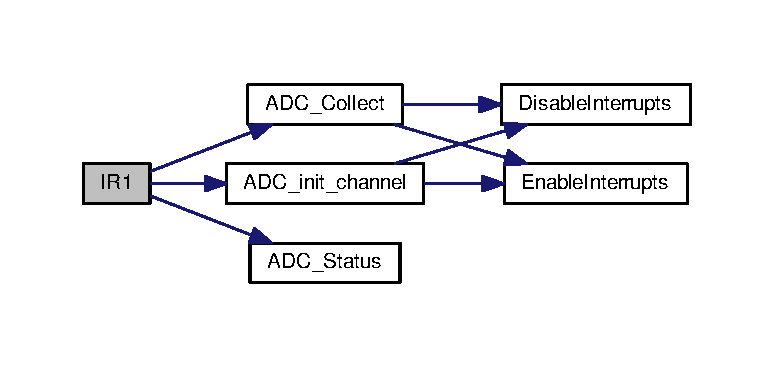
\includegraphics[width=350pt]{_lab6_8c_a93e4ea9d9ef2ee60af1459a12b6e6d4c_cgraph}
\end{center}
\end{figure}




Here is the caller graph for this function\-:
\nopagebreak
\begin{figure}[H]
\begin{center}
\leavevmode
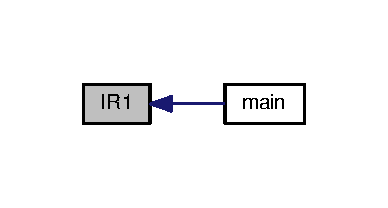
\includegraphics[width=186pt]{_lab6_8c_a93e4ea9d9ef2ee60af1459a12b6e6d4c_icgraph}
\end{center}
\end{figure}


\hypertarget{_lab6_8c_adc674087543a04e8700d2427322b8328}{\index{Lab6.\-c@{Lab6.\-c}!I\-R2@{I\-R2}}
\index{I\-R2@{I\-R2}!Lab6.c@{Lab6.\-c}}
\subsubsection[{I\-R2}]{\setlength{\rightskip}{0pt plus 5cm}void I\-R2 (
\begin{DoxyParamCaption}
\item[{void}]{}
\end{DoxyParamCaption}
)}}\label{_lab6_8c_adc674087543a04e8700d2427322b8328}


Definition at line 366 of file Lab6.\-c.


\begin{DoxyCode}
366               \{
367         
368   uint32\_t SendData;
369   CanMessage\_t msg;
370     uint8\_t byteMe[5];
371   \hyperlink{_a_d_c_8c_ae7cef9ecd73d25c0931372d21e6be943}{ADC\_init\_channel}(2, 100);
372     \textcolor{keywordflow}{while}(1)\{
373         SendData = 0;
374         OS\_Wait(&\hyperlink{_lab6_8c_a0b7ebdb20b3f7f2953b0f661bc81b3d4}{ADC\_Collection});
375     \hyperlink{_a_d_c_8c_a9fdea7e06f4c4769ab22981dafb58477}{ADC\_Collect}(2, 100, \hyperlink{_lab6_8c_a6a20659f3190002cee79b8ee18b012a7}{Res\_buffer2}, 2*\hyperlink{_lab6_8c_ab414aa8e1ca870685c1cf52fb815c718}{buffSIZE}); \textcolor{comment}{//128, to bring down
       sampling rate from 100 to 50}
376     \textcolor{keywordflow}{while}(\hyperlink{_a_d_c_8c_ab991147608f978ac77baf774334e802b}{ADC\_Status}(2))\{\}
377     OS\_Signal(&\hyperlink{_lab6_8c_a0b7ebdb20b3f7f2953b0f661bc81b3d4}{ADC\_Collection});
378         \textcolor{keywordflow}{for}(\textcolor{keywordtype}{int} i = 0; i < \hyperlink{_lab6_8c_ab414aa8e1ca870685c1cf52fb815c718}{buffSIZE}-MEDIAN\_FILTER\_SIZE; i++)\{
379       SendData += median\_filt(&\hyperlink{_lab6_8c_a6a20659f3190002cee79b8ee18b012a7}{Res\_buffer2}[i]);
380     \}
381     SendData = SendData/(\hyperlink{_lab6_8c_ab414aa8e1ca870685c1cf52fb815c718}{buffSIZE}-MEDIAN\_FILTER\_SIZE);
382 \textcolor{comment}{//    msg.mId = IR\_2\_ID;}
383 \textcolor{comment}{//    msg.data = SendData;}
384 \textcolor{comment}{//        CanMessage2Buff(&msg, byteMe);}
385 \textcolor{comment}{//    CAN0\_SendData(byteMe);}
386 \textcolor{comment}{//    }
387     \hyperlink{_lab6_8c_a2b37f85b4e04e07d733d0925cafeea88}{IR2Val} = SendData; 
388     \textcolor{comment}{//LEDS = BLUE;}
389   \}
390   OS\_Kill();
391 \}
\end{DoxyCode}


Here is the call graph for this function\-:
\nopagebreak
\begin{figure}[H]
\begin{center}
\leavevmode
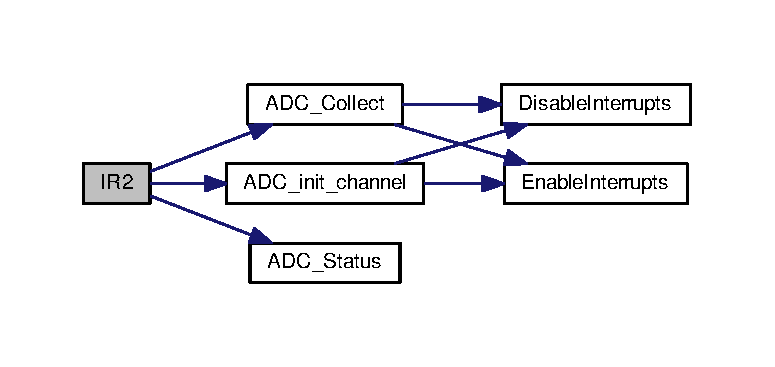
\includegraphics[width=350pt]{_lab6_8c_adc674087543a04e8700d2427322b8328_cgraph}
\end{center}
\end{figure}




Here is the caller graph for this function\-:
\nopagebreak
\begin{figure}[H]
\begin{center}
\leavevmode
\includegraphics[width=186pt]{_lab6_8c_adc674087543a04e8700d2427322b8328_icgraph}
\end{center}
\end{figure}


\hypertarget{_lab6_8c_a7c8ab9e9d2256a9f7ecee8fb0499cb91}{\index{Lab6.\-c@{Lab6.\-c}!I\-R3@{I\-R3}}
\index{I\-R3@{I\-R3}!Lab6.c@{Lab6.\-c}}
\subsubsection[{I\-R3}]{\setlength{\rightskip}{0pt plus 5cm}void I\-R3 (
\begin{DoxyParamCaption}
\item[{void}]{}
\end{DoxyParamCaption}
)}}\label{_lab6_8c_a7c8ab9e9d2256a9f7ecee8fb0499cb91}


Definition at line 394 of file Lab6.\-c.


\begin{DoxyCode}
394               \{
395   uint32\_t SendData;
396   CanMessage\_t msg;
397     uint8\_t byteMe[5];
398   \hyperlink{_a_d_c_8c_ae7cef9ecd73d25c0931372d21e6be943}{ADC\_init\_channel}(4, 100);
399     \textcolor{keywordflow}{while}(1)\{
400         SendData = 0;
401         OS\_Wait(&\hyperlink{_lab6_8c_a0b7ebdb20b3f7f2953b0f661bc81b3d4}{ADC\_Collection});
402     \hyperlink{_a_d_c_8c_a9fdea7e06f4c4769ab22981dafb58477}{ADC\_Collect}(4, 100, \hyperlink{_lab6_8c_ad382a86c210687cdebcb99093927c7d3}{Res\_buffer3}, 2*\hyperlink{_lab6_8c_ab414aa8e1ca870685c1cf52fb815c718}{buffSIZE}); \textcolor{comment}{//128, to bring down
       sampling rate from 100 to 50}
403     \textcolor{keywordflow}{while}(\hyperlink{_a_d_c_8c_ab991147608f978ac77baf774334e802b}{ADC\_Status}(3))\{\}
404         OS\_Signal(&\hyperlink{_lab6_8c_a0b7ebdb20b3f7f2953b0f661bc81b3d4}{ADC\_Collection});
405     \textcolor{keywordflow}{for}(\textcolor{keywordtype}{int} i = 0; i < \hyperlink{_lab6_8c_ab414aa8e1ca870685c1cf52fb815c718}{buffSIZE}-MEDIAN\_FILTER\_SIZE; i++)\{
406       SendData += median\_filt(&\hyperlink{_lab6_8c_ad382a86c210687cdebcb99093927c7d3}{Res\_buffer3}[i]);
407     \}
408     SendData = SendData/(\hyperlink{_lab6_8c_ab414aa8e1ca870685c1cf52fb815c718}{buffSIZE}-MEDIAN\_FILTER\_SIZE);
409 \textcolor{comment}{//    msg.mId = IR\_3\_ID;}
410 \textcolor{comment}{//    msg.data = SendData;}
411 \textcolor{comment}{//        CanMessage2Buff(&msg, byteMe);}
412 \textcolor{comment}{//    CAN0\_SendData(byteMe);}
413     \hyperlink{_lab6_8c_a6af4ef6e3413367b368acb7b5ba47d17}{IR3Val} = SendData; 
414     \textcolor{comment}{//LEDS = RED;}
415   \}
416   OS\_Kill();
417 \}
\end{DoxyCode}


Here is the call graph for this function\-:
\nopagebreak
\begin{figure}[H]
\begin{center}
\leavevmode
\includegraphics[width=350pt]{_lab6_8c_a7c8ab9e9d2256a9f7ecee8fb0499cb91_cgraph}
\end{center}
\end{figure}




Here is the caller graph for this function\-:
\nopagebreak
\begin{figure}[H]
\begin{center}
\leavevmode
\includegraphics[width=186pt]{_lab6_8c_a7c8ab9e9d2256a9f7ecee8fb0499cb91_icgraph}
\end{center}
\end{figure}


\hypertarget{_lab6_8c_a840291bc02cba5474a4cb46a9b9566fe}{\index{Lab6.\-c@{Lab6.\-c}!main@{main}}
\index{main@{main}!Lab6.c@{Lab6.\-c}}
\subsubsection[{main}]{\setlength{\rightskip}{0pt plus 5cm}int main (
\begin{DoxyParamCaption}
\item[{void}]{}
\end{DoxyParamCaption}
)}}\label{_lab6_8c_a840291bc02cba5474a4cb46a9b9566fe}


Definition at line 924 of file Lab6.\-c.


\begin{DoxyCode}
924               \{   \textcolor{comment}{// testmain1}
925   OS\_Init();           \textcolor{comment}{// initialize, disable interrupts}
926 \textcolor{comment}{//  PWM0Dual\_Period(40000);           // 12.50 Hz, 15 RPM}
927   \hyperlink{_lab6_8c_ae19ef8807dc64129635da5b3b781588a}{PortF\_Init}();
928   CAN0\_Open();
929 
930   PWM0Dual\_Init(60000);            \textcolor{comment}{// initialize PWM1-0, 0.8333 Hz, 1 RPM}
931   NumCreated = 0 ;
932   \textcolor{comment}{// create initial foreground threads}
933   NumCreated += OS\_AddThread(&\hyperlink{_lab6_8c_a43617af71ca5f26b8d87c7460ee110f4}{CAN\_Listener}, 128, 2);
934   \textcolor{comment}{//NumCreated += OS\_AddThread(&Controller2, 128, 2);}
935   NumCreated += OS\_AddThread(&\hyperlink{_lab6_8c_a8df88b108bf75863b97b46c603310d3c}{Controller}, 128, 2);
936   OS\_InitSemaphore(&\hyperlink{_lab6_8c_a0b7ebdb20b3f7f2953b0f661bc81b3d4}{ADC\_Collection}, 1);
937   NumCreated += OS\_AddThread(&\hyperlink{_lab6_8c_a93e4ea9d9ef2ee60af1459a12b6e6d4c}{IR1}, 128, 2);
938   NumCreated += OS\_AddThread(&\hyperlink{_lab6_8c_adc674087543a04e8700d2427322b8328}{IR2}, 128, 2);
939   NumCreated += OS\_AddThread(&\hyperlink{_lab6_8c_a7c8ab9e9d2256a9f7ecee8fb0499cb91}{IR3}, 128, 2);
940   OS\_Launch(TIME\_1MS/4); \textcolor{comment}{// doesn't return, interrupts enabled in here}
941   OS\_AddPeriodicThread(&\hyperlink{_lab6_8c_a968e17f037bc1e2ec26307388d6d17ad}{deathRay},10*TIME\_1MS,0);   \textcolor{comment}{// time out routines for disk}
942   \textcolor{keywordflow}{return} 0;               \textcolor{comment}{// this never executes}
943 \}
\end{DoxyCode}


Here is the call graph for this function\-:
\nopagebreak
\begin{figure}[H]
\begin{center}
\leavevmode
\includegraphics[width=350pt]{_lab6_8c_a840291bc02cba5474a4cb46a9b9566fe_cgraph}
\end{center}
\end{figure}


\hypertarget{_lab6_8c_a03c7899f3ff55164dfc955aed1b328f8}{\index{Lab6.\-c@{Lab6.\-c}!Ping1@{Ping1}}
\index{Ping1@{Ping1}!Lab6.c@{Lab6.\-c}}
\subsubsection[{Ping1}]{\setlength{\rightskip}{0pt plus 5cm}uint32\-\_\-t Ping1 (
\begin{DoxyParamCaption}
\item[{void}]{}
\end{DoxyParamCaption}
)}}\label{_lab6_8c_a03c7899f3ff55164dfc955aed1b328f8}


Definition at line 181 of file Lab6.\-c.


\begin{DoxyCode}
181                     \{
182     \textcolor{comment}{// uint32\_t pingStartTime; }
183     \textcolor{comment}{// uint32\_t pingEndTime;}
184     \textcolor{comment}{//Write GPIO\_Pin High}
185     \textcolor{keywordtype}{long} sr = \hyperlink{_lab6_8c_a6e7e2088607214bc15b17ac57b57df1b}{StartCritical}();
186   \hyperlink{_lab6_8c_ad55f1ce2962d3a43aeed74b5459214f6}{PA7} = 0x80;
187     OS\_DelayUS(5);
188     \textcolor{comment}{//Write GPIO Pin Low}
189     \hyperlink{_lab6_8c_ad55f1ce2962d3a43aeed74b5459214f6}{PA7} = 0x00;
190     \textcolor{comment}{//Could move into a ISR}
191     \textcolor{comment}{//while(gpio\_Pin\_Low)\{\}}
192     \textcolor{comment}{// while(PA6 == 0)\{\}}
193     \textcolor{comment}{// pingStartTime = OS\_GetUsTime();}
194 
195     \textcolor{comment}{// //while(gpio\_Pin\_High)\{\}}
196     \textcolor{comment}{// while(PA6 != 0)\{\}}
197 
198     \textcolor{comment}{// pingEndTime = OS\_GetUsTime();}
199     \textcolor{comment}{// OS\_DelayUS(200);}
200     \textcolor{comment}{// //Speed of sound in air is approx c = 343 m/s = 340 m/s * 1000m.0m/m * (1s/100000us)}
201     \textcolor{comment}{// //Then the ping time is c*dT/2}
202         \hyperlink{_lab6_8c_a670da3ff1aea0c7d54c40e9e40b5eeed}{EndCritical}(sr);
203     \textcolor{comment}{// return ((pingEndTime - pingStartTime) /*>> 1*/)*34300/1000000;}
204 
205   uint32\_t delta;
206   \hyperlink{_lab6_8c_a6b0304a7c2f611c97a1f4779a9bfb483}{Ping1Mail}.Receive(delta);
207   \textcolor{keywordflow}{return} delta;
208 \}
\end{DoxyCode}


Here is the call graph for this function\-:
\nopagebreak
\begin{figure}[H]
\begin{center}
\leavevmode
\includegraphics[width=226pt]{_lab6_8c_a03c7899f3ff55164dfc955aed1b328f8_cgraph}
\end{center}
\end{figure}




Here is the caller graph for this function\-:
\nopagebreak
\begin{figure}[H]
\begin{center}
\leavevmode
\includegraphics[width=202pt]{_lab6_8c_a03c7899f3ff55164dfc955aed1b328f8_icgraph}
\end{center}
\end{figure}


\hypertarget{_lab6_8c_a88c85cf0752512429969dbc0b75626d0}{\index{Lab6.\-c@{Lab6.\-c}!Ping2@{Ping2}}
\index{Ping2@{Ping2}!Lab6.c@{Lab6.\-c}}
\subsubsection[{Ping2}]{\setlength{\rightskip}{0pt plus 5cm}uint32\-\_\-t Ping2 (
\begin{DoxyParamCaption}
\item[{void}]{}
\end{DoxyParamCaption}
)}}\label{_lab6_8c_a88c85cf0752512429969dbc0b75626d0}


Definition at line 218 of file Lab6.\-c.


\begin{DoxyCode}
218                     \{
219   \textcolor{comment}{// uint32\_t pingStartTime; }
220   \textcolor{comment}{// uint32\_t pingEndTime;}
221   \textcolor{comment}{//Write GPIO\_Pin High}
222     \textcolor{keywordtype}{long} sr = \hyperlink{_lab6_8c_a6e7e2088607214bc15b17ac57b57df1b}{StartCritical}();
223   \hyperlink{_lab6_8c_a1194403dd24b90c5af73482c52ad1360}{PC7} = 0x80;
224   OS\_DelayUS(5);
225   \textcolor{comment}{//Write GPIO Pin Low}
226   \hyperlink{_lab6_8c_a1194403dd24b90c5af73482c52ad1360}{PC7} = 0x00;
227   \textcolor{comment}{//Could move into a ISR}
228   \textcolor{comment}{//while(gpio\_Pin\_Low)\{\}}
229   \textcolor{comment}{// while(PC6 == 0)\{\}}
230   \textcolor{comment}{// pingStartTime = OS\_GetUsTime();}
231 
232   \textcolor{comment}{// //while(gpio\_Pin\_High)\{\}}
233   \textcolor{comment}{// while(PC6 != 0)\{\}}
234 
235     \hyperlink{_lab6_8c_a670da3ff1aea0c7d54c40e9e40b5eeed}{EndCritical}(sr);
236 
237   \textcolor{comment}{// pingEndTime = OS\_GetUsTime();}
238   \textcolor{comment}{// OS\_DelayUS(200);}
239   \textcolor{comment}{// //Speed of sound in air is approx c = 343 m/s = 340 m/s * 1000m.0m/m * (1s/100000us)}
240   \textcolor{comment}{// //Then the ping time is c*dT/2}
241   \textcolor{comment}{// return ((pingEndTime - pingStartTime) /*>> 1*/)*34300/1000000;}
242   uint32\_t delta;
243   \hyperlink{_lab6_8c_a39dbfc1fca14892a7d8916d445fb4321}{Ping2Mail}.Receive(delta);
244   \textcolor{keywordflow}{return} delta;
245 \}
\end{DoxyCode}


Here is the call graph for this function\-:
\nopagebreak
\begin{figure}[H]
\begin{center}
\leavevmode
\includegraphics[width=226pt]{_lab6_8c_a88c85cf0752512429969dbc0b75626d0_cgraph}
\end{center}
\end{figure}




Here is the caller graph for this function\-:
\nopagebreak
\begin{figure}[H]
\begin{center}
\leavevmode
\includegraphics[width=200pt]{_lab6_8c_a88c85cf0752512429969dbc0b75626d0_icgraph}
\end{center}
\end{figure}


\hypertarget{_lab6_8c_acbb551322fcba7749c8c40006cd9ffd8}{\index{Lab6.\-c@{Lab6.\-c}!Ping\-L@{Ping\-L}}
\index{Ping\-L@{Ping\-L}!Lab6.c@{Lab6.\-c}}
\subsubsection[{Ping\-L}]{\setlength{\rightskip}{0pt plus 5cm}void Ping\-L (
\begin{DoxyParamCaption}
\item[{void}]{}
\end{DoxyParamCaption}
)}}\label{_lab6_8c_acbb551322fcba7749c8c40006cd9ffd8}


Definition at line 273 of file Lab6.\-c.


\begin{DoxyCode}
273                 \{
274   
275   uint32\_t distance;
276   CanMessage\_t msg;
277     uint8\_t byteMe[5];
278 
279   uint32\_t i = 0;
280   \textcolor{keywordflow}{while}(1)\{
281     distance = 0;
282     \textcolor{keywordflow}{for}(i = 0; i < 4; i++)\{
283       distance += \hyperlink{_lab6_8c_a88c85cf0752512429969dbc0b75626d0}{Ping2}();
284     \}
285     distance = distance >> 2;
286     \textcolor{comment}{//XmtData = (uint8\_t *) &distance;}
287     msg.mId = \hyperlink{_lab6_8c_a25b36259b474d6e7ff4c3eb00374f947}{PING\_L\_ID};
288     msg.data = distance;
289         CanMessage2Buff(&msg, byteMe);
290 
291     \textcolor{comment}{//CAN0\_SendData(CAST\_CAN\_2\_UINT8P(msg));}
292         CAN0\_SendData(byteMe);
293 
294 
295   \}
296   OS\_Kill();
297 \}
\end{DoxyCode}


Here is the call graph for this function\-:
\nopagebreak
\begin{figure}[H]
\begin{center}
\leavevmode
\includegraphics[width=304pt]{_lab6_8c_acbb551322fcba7749c8c40006cd9ffd8_cgraph}
\end{center}
\end{figure}


\hypertarget{_lab6_8c_abd66255c87de5710737f979da785c171}{\index{Lab6.\-c@{Lab6.\-c}!Ping\-R@{Ping\-R}}
\index{Ping\-R@{Ping\-R}!Lab6.c@{Lab6.\-c}}
\subsubsection[{Ping\-R}]{\setlength{\rightskip}{0pt plus 5cm}void Ping\-R (
\begin{DoxyParamCaption}
\item[{void}]{}
\end{DoxyParamCaption}
)}}\label{_lab6_8c_abd66255c87de5710737f979da785c171}


Definition at line 247 of file Lab6.\-c.


\begin{DoxyCode}
247                 \{
248   
249 
250   uint32\_t distance;
251   CanMessage\_t msg;
252     uint8\_t byteMe[5];
253 
254   \textcolor{comment}{//uint32\_t distance\_buff[4];}
255   \textcolor{keywordtype}{unsigned} \textcolor{keywordtype}{long} \textcolor{keywordtype}{id} = OS\_Id();
256   uint32\_t i = 0;
257   \textcolor{keywordflow}{while}(1)\{
258     distance = 0;
259     \textcolor{keywordflow}{for}(i = 0; i < 4; i++)\{
260       distance += \hyperlink{_lab6_8c_a03c7899f3ff55164dfc955aed1b328f8}{Ping1}();
261     \}
262     distance = distance >> 2;
263     \textcolor{comment}{//XmtData = (uint8\_t *) &distance;}
264     msg.mId = \hyperlink{_lab6_8c_a0d2937f7ce6f0370010af0183f2cfb24}{PING\_R\_ID};
265     msg.data = distance;
266         CanMessage2Buff(&msg, byteMe);
267     CAN0\_SendData(byteMe);
268 
269   \}
270   OS\_Kill();
271 \}
\end{DoxyCode}


Here is the call graph for this function\-:
\nopagebreak
\begin{figure}[H]
\begin{center}
\leavevmode
\includegraphics[width=306pt]{_lab6_8c_abd66255c87de5710737f979da785c171_cgraph}
\end{center}
\end{figure}


\hypertarget{_lab6_8c_ac079e51ee4b2d6294323419435982b5d}{\index{Lab6.\-c@{Lab6.\-c}!Port\-A\-\_\-\-Sensor\-Board\-\_\-\-Init@{Port\-A\-\_\-\-Sensor\-Board\-\_\-\-Init}}
\index{Port\-A\-\_\-\-Sensor\-Board\-\_\-\-Init@{Port\-A\-\_\-\-Sensor\-Board\-\_\-\-Init}!Lab6.c@{Lab6.\-c}}
\subsubsection[{Port\-A\-\_\-\-Sensor\-Board\-\_\-\-Init}]{\setlength{\rightskip}{0pt plus 5cm}void Port\-A\-\_\-\-Sensor\-Board\-\_\-\-Init (
\begin{DoxyParamCaption}
\item[{void}]{}
\end{DoxyParamCaption}
)}}\label{_lab6_8c_ac079e51ee4b2d6294323419435982b5d}


Definition at line 161 of file Lab6.\-c.


\begin{DoxyCode}
161                                  \{ \textcolor{keywordtype}{unsigned} \textcolor{keywordtype}{long} \textcolor{keyword}{volatile} delay;
162   \textcolor{comment}{//SYSCTL\_RCGC2\_R |= 0x10;       // activate port A}
163   SYSCTL\_RCGCGPIO\_R |= 0x01;       
164   delay = SYSCTL\_RCGC2\_R;        
165   delay = SYSCTL\_RCGC2\_R;         
166   GPIO\_PORTA\_DIR\_R |= 0xC0;    \textcolor{comment}{// make PA7 output}
167   GPIO\_PORTA\_DIR\_R &= ~0x40;   \textcolor{comment}{//PA6 is echo}
168   GPIO\_PORTA\_AFSEL\_R &= ~0xC0;   \textcolor{comment}{// disable alt funct on PA6-7}
169   GPIO\_PORTA\_DEN\_R |= 0xC0;     \textcolor{comment}{// enable digital I/O on PA6-7}
170 
171   GPIO\_PORTA\_IS\_R &= ~(1 << 6);   \textcolor{comment}{// PA6 is edge-sensitive}
172   GPIO\_PORTA\_IBE\_R |= (1 << 6);   \textcolor{comment}{// PA6 is sensitive to both edges}
173   GPIO\_PORTA\_IEV\_R |= (1 << 6);   \textcolor{comment}{// PA6 rising edge event (Dont care)}
174   GPIO\_PORTA\_ICR\_R = (1 << 6); \textcolor{comment}{//Clear the flag}
175   GPIO\_PORTA\_IM\_R |= (1 << 6);    \textcolor{comment}{// enable interrupt on PA6}
176 
177   \textcolor{comment}{//Priority Level 3}
178   NVIC\_PRI0\_R = (NVIC\_PRI0\_R&0xFFFFFFF00)| (3 << 5);
179   NVIC\_EN0\_R = 1 << 0;
180 \}
\end{DoxyCode}
\hypertarget{_lab6_8c_a5a2a2db7e83737739f577faafdf8cce7}{\index{Lab6.\-c@{Lab6.\-c}!Port\-C\-\_\-\-Sensor\-Board\-\_\-\-Init@{Port\-C\-\_\-\-Sensor\-Board\-\_\-\-Init}}
\index{Port\-C\-\_\-\-Sensor\-Board\-\_\-\-Init@{Port\-C\-\_\-\-Sensor\-Board\-\_\-\-Init}!Lab6.c@{Lab6.\-c}}
\subsubsection[{Port\-C\-\_\-\-Sensor\-Board\-\_\-\-Init}]{\setlength{\rightskip}{0pt plus 5cm}void Port\-C\-\_\-\-Sensor\-Board\-\_\-\-Init (
\begin{DoxyParamCaption}
\item[{void}]{}
\end{DoxyParamCaption}
)}}\label{_lab6_8c_a5a2a2db7e83737739f577faafdf8cce7}


Definition at line 140 of file Lab6.\-c.


\begin{DoxyCode}
140                                  \{ \textcolor{keywordtype}{unsigned} \textcolor{keywordtype}{long} \textcolor{keyword}{volatile} delay;
141   \textcolor{comment}{//SYSCTL\_RCGC2\_R |= 0x10;       // activate port c}
142   SYSCTL\_RCGCGPIO\_R |= 0x04;       
143   delay = SYSCTL\_RCGC2\_R;        
144   delay = SYSCTL\_RCGC2\_R;         
145   GPIO\_PORTC\_DIR\_R |= 0xC0;    \textcolor{comment}{// make PC7 output}
146   GPIO\_PORTC\_DIR\_R &= ~0x40;   \textcolor{comment}{//PC6 is echo}
147   GPIO\_PORTC\_AFSEL\_R &= ~0xC0;   \textcolor{comment}{// disable alt funct on PC6-7}
148   GPIO\_PORTC\_DEN\_R |= 0xC0;     \textcolor{comment}{// enable digital I/O on PC6-7}
149 
150   GPIO\_PORTC\_IS\_R &= ~(1 << 6);   \textcolor{comment}{// PA6 is edge-sensitive}
151   GPIO\_PORTC\_IBE\_R |= (1 << 6);   \textcolor{comment}{// PA6 is sensitive to both edges}
152   GPIO\_PORTC\_IEV\_R |= (1 << 6);   \textcolor{comment}{// PA6 rising edge event (Dont care)}
153   GPIO\_PORTC\_ICR\_R = (1 << 6); \textcolor{comment}{//Clear the flag}
154   GPIO\_PORTC\_IM\_R |= (1 << 6);    \textcolor{comment}{// enable interrupt on PA6}
155 
156   \textcolor{comment}{//Priority Level 3}
157   NVIC\_PRI0\_R = (NVIC\_PRI0\_R&0xFF00FFFFF)| (1 << 21);
158   NVIC\_EN0\_R = 1 << 2;
159 \}
\end{DoxyCode}
\hypertarget{_lab6_8c_a04369a3281263e369b0cffb5658b24e3}{\index{Lab6.\-c@{Lab6.\-c}!Port\-D\-\_\-\-Init@{Port\-D\-\_\-\-Init}}
\index{Port\-D\-\_\-\-Init@{Port\-D\-\_\-\-Init}!Lab6.c@{Lab6.\-c}}
\subsubsection[{Port\-D\-\_\-\-Init}]{\setlength{\rightskip}{0pt plus 5cm}void Port\-D\-\_\-\-Init (
\begin{DoxyParamCaption}
\item[{void}]{}
\end{DoxyParamCaption}
)}}\label{_lab6_8c_a04369a3281263e369b0cffb5658b24e3}


Definition at line 87 of file Lab6.\-c.


\begin{DoxyCode}
87                      \{ \textcolor{keywordtype}{unsigned} \textcolor{keywordtype}{long} \textcolor{keyword}{volatile} delay;
88   \textcolor{comment}{//SYSCTL\_RCGC2\_R |= 0x10;       // activate port D}
89   SYSCTL\_RCGCGPIO\_R |= 0x08;       
90   delay = SYSCTL\_RCGC2\_R;        
91   delay = SYSCTL\_RCGC2\_R;         
92   GPIO\_PORTD\_DIR\_R |= 0xC0;    \textcolor{comment}{// make PD7 output}
93     GPIO\_PORTD\_DIR\_R &= ~0x40;   \textcolor{comment}{//PD6 is echo}
94   GPIO\_PORTD\_AFSEL\_R &= ~0xC0;   \textcolor{comment}{// disable alt funct on PD6-7}
95   GPIO\_PORTD\_DEN\_R |= 0xC0;     \textcolor{comment}{// enable digital I/O on PD6-7}
96   \textcolor{comment}{//GPIO\_PORTD\_PCTL\_R = ~0x0000FFFF;}
97   \textcolor{comment}{//GPIO\_PORTD\_AMSEL\_R &= ~0x0F;;      // disable analog functionality on PF}
98   GPIO\_PORTD\_IS\_R &= ~(1 << 6);   \textcolor{comment}{// PD6 is edge-sensitive}
99   GPIO\_PORTD\_IBE\_R |= (1 << 6);   \textcolor{comment}{// PD6 is sensitive to both edges}
100   GPIO\_PORTD\_IEV\_R |= (1 << 6);   \textcolor{comment}{// PD6 rising edge event (Dont care)}
101   GPIO\_PORTD\_ICR\_R = (1 << 6); \textcolor{comment}{//Clear the flag}
102   GPIO\_PORTD\_IM\_R |= (1 << 6);    \textcolor{comment}{// enable interrupt on PD6}
103 
104   \textcolor{comment}{//Priority Level 3}
105   NVIC\_PRI0\_R = (NVIC\_PRI0\_R&0x00FFFFFF)| (0 << 29);
106   NVIC\_EN0\_R = 1 << 3;
107  
108 \}
\end{DoxyCode}
\hypertarget{_lab6_8c_ae19ef8807dc64129635da5b3b781588a}{\index{Lab6.\-c@{Lab6.\-c}!Port\-F\-\_\-\-Init@{Port\-F\-\_\-\-Init}}
\index{Port\-F\-\_\-\-Init@{Port\-F\-\_\-\-Init}!Lab6.c@{Lab6.\-c}}
\subsubsection[{Port\-F\-\_\-\-Init}]{\setlength{\rightskip}{0pt plus 5cm}void Port\-F\-\_\-\-Init (
\begin{DoxyParamCaption}
\item[{void}]{}
\end{DoxyParamCaption}
)}}\label{_lab6_8c_ae19ef8807dc64129635da5b3b781588a}


Definition at line 424 of file Lab6.\-c.


\begin{DoxyCode}
424                      \{
425   SYSCTL\_RCGCGPIO\_R |= 0x20;       \textcolor{comment}{// activate port F}
426   \textcolor{keywordflow}{while}((SYSCTL\_PRGPIO\_R&0x0020) == 0)\{\};\textcolor{comment}{// ready?}
427   GPIO\_PORTF\_DIR\_R |= 0x0E;        \textcolor{comment}{// make PF3-1 output (PF3-1 built-in LEDs)}
428   GPIO\_PORTF\_AFSEL\_R &= ~0x0E;     \textcolor{comment}{// disable alt funct on PF3-1}
429   GPIO\_PORTF\_DEN\_R |= 0x0E;        \textcolor{comment}{// enable digital I/O on PF3-1}
430                                    \textcolor{comment}{// configure PF3-1 as GPIO}
431   GPIO\_PORTF\_PCTL\_R = (GPIO\_PORTF\_PCTL\_R&0xFFFF000F)+0x00000000;
432   GPIO\_PORTF\_AMSEL\_R = 0;          \textcolor{comment}{// disable analog functionality on PF}
433   \hyperlink{_lab6_8c_a61686d33603491344883775b9b31e172}{LEDS} = 0;     \textcolor{comment}{// turn all LEDs off}
434 \}
\end{DoxyCode}


Here is the caller graph for this function\-:
\nopagebreak
\begin{figure}[H]
\begin{center}
\leavevmode
\includegraphics[width=214pt]{_lab6_8c_ae19ef8807dc64129635da5b3b781588a_icgraph}
\end{center}
\end{figure}


\hypertarget{_lab6_8c_a6e7e2088607214bc15b17ac57b57df1b}{\index{Lab6.\-c@{Lab6.\-c}!Start\-Critical@{Start\-Critical}}
\index{Start\-Critical@{Start\-Critical}!Lab6.c@{Lab6.\-c}}
\subsubsection[{Start\-Critical}]{\setlength{\rightskip}{0pt plus 5cm}long Start\-Critical (
\begin{DoxyParamCaption}
\item[{void}]{}
\end{DoxyParamCaption}
)}}\label{_lab6_8c_a6e7e2088607214bc15b17ac57b57df1b}


Here is the caller graph for this function\-:
\nopagebreak
\begin{figure}[H]
\begin{center}
\leavevmode
\includegraphics[width=306pt]{_lab6_8c_a6e7e2088607214bc15b17ac57b57df1b_icgraph}
\end{center}
\end{figure}


\hypertarget{_lab6_8c_a80ae22f2f73496246542c428c4bec38f}{\index{Lab6.\-c@{Lab6.\-c}!Wait\-For\-Interrupt@{Wait\-For\-Interrupt}}
\index{Wait\-For\-Interrupt@{Wait\-For\-Interrupt}!Lab6.c@{Lab6.\-c}}
\subsubsection[{Wait\-For\-Interrupt}]{\setlength{\rightskip}{0pt plus 5cm}void Wait\-For\-Interrupt (
\begin{DoxyParamCaption}
\item[{void}]{}
\end{DoxyParamCaption}
)}}\label{_lab6_8c_a80ae22f2f73496246542c428c4bec38f}


\subsection{Variable Documentation}
\hypertarget{_lab6_8c_a0b7ebdb20b3f7f2953b0f661bc81b3d4}{\index{Lab6.\-c@{Lab6.\-c}!A\-D\-C\-\_\-\-Collection@{A\-D\-C\-\_\-\-Collection}}
\index{A\-D\-C\-\_\-\-Collection@{A\-D\-C\-\_\-\-Collection}!Lab6.c@{Lab6.\-c}}
\subsubsection[{A\-D\-C\-\_\-\-Collection}]{\setlength{\rightskip}{0pt plus 5cm}Sema4\-Type A\-D\-C\-\_\-\-Collection}}\label{_lab6_8c_a0b7ebdb20b3f7f2953b0f661bc81b3d4}


Definition at line 62 of file Lab6.\-c.

\hypertarget{_lab6_8c_aca879141a9e2660e4cd8e410208fc1ec}{\index{Lab6.\-c@{Lab6.\-c}!front\-Error@{front\-Error}}
\index{front\-Error@{front\-Error}!Lab6.c@{Lab6.\-c}}
\subsubsection[{front\-Error}]{\setlength{\rightskip}{0pt plus 5cm}float front\-Error = 0}}\label{_lab6_8c_aca879141a9e2660e4cd8e410208fc1ec}


Definition at line 540 of file Lab6.\-c.

\hypertarget{_lab6_8c_a08f684c971e5e14bcd9ded712ffc8e31}{\index{Lab6.\-c@{Lab6.\-c}!front\-Highest\-Speed@{front\-Highest\-Speed}}
\index{front\-Highest\-Speed@{front\-Highest\-Speed}!Lab6.c@{Lab6.\-c}}
\subsubsection[{front\-Highest\-Speed}]{\setlength{\rightskip}{0pt plus 5cm}int front\-Highest\-Speed = 250}}\label{_lab6_8c_a08f684c971e5e14bcd9ded712ffc8e31}


Definition at line 545 of file Lab6.\-c.

\hypertarget{_lab6_8c_a4e5311a153c7dc8b2e6160e3733ddb4d}{\index{Lab6.\-c@{Lab6.\-c}!front\-Low\-Cap@{front\-Low\-Cap}}
\index{front\-Low\-Cap@{front\-Low\-Cap}!Lab6.c@{Lab6.\-c}}
\subsubsection[{front\-Low\-Cap}]{\setlength{\rightskip}{0pt plus 5cm}int front\-Low\-Cap = 10}}\label{_lab6_8c_a4e5311a153c7dc8b2e6160e3733ddb4d}


Definition at line 549 of file Lab6.\-c.

\hypertarget{_lab6_8c_a5fa41fb37330973b00a53519b43dc652}{\index{Lab6.\-c@{Lab6.\-c}!front\-Lowest\-Speed@{front\-Lowest\-Speed}}
\index{front\-Lowest\-Speed@{front\-Lowest\-Speed}!Lab6.c@{Lab6.\-c}}
\subsubsection[{front\-Lowest\-Speed}]{\setlength{\rightskip}{0pt plus 5cm}int front\-Lowest\-Speed = 190}}\label{_lab6_8c_a5fa41fb37330973b00a53519b43dc652}


Definition at line 547 of file Lab6.\-c.

\hypertarget{_lab6_8c_a3a69578ffb800441a624e2411824678a}{\index{Lab6.\-c@{Lab6.\-c}!front\-Threashold@{front\-Threashold}}
\index{front\-Threashold@{front\-Threashold}!Lab6.c@{Lab6.\-c}}
\subsubsection[{front\-Threashold}]{\setlength{\rightskip}{0pt plus 5cm}float front\-Threashold = 600}}\label{_lab6_8c_a3a69578ffb800441a624e2411824678a}


Definition at line 519 of file Lab6.\-c.

\hypertarget{_lab6_8c_ac17b395804882db11d8bd30dd0d5c9be}{\index{Lab6.\-c@{Lab6.\-c}!go\-Straight@{go\-Straight}}
\index{go\-Straight@{go\-Straight}!Lab6.c@{Lab6.\-c}}
\subsubsection[{go\-Straight}]{\setlength{\rightskip}{0pt plus 5cm}bool go\-Straight = 0}}\label{_lab6_8c_ac17b395804882db11d8bd30dd0d5c9be}


Definition at line 543 of file Lab6.\-c.

\hypertarget{_lab6_8c_ab639d295e81c2bcff1a343f7cc1273f7}{\index{Lab6.\-c@{Lab6.\-c}!high\-Correction\-Cap@{high\-Correction\-Cap}}
\index{high\-Correction\-Cap@{high\-Correction\-Cap}!Lab6.c@{Lab6.\-c}}
\subsubsection[{high\-Correction\-Cap}]{\setlength{\rightskip}{0pt plus 5cm}float high\-Correction\-Cap = {\bf highest\-Speed} $\ast$(1 -\/ {\bf lowest\-P})}}\label{_lab6_8c_ab639d295e81c2bcff1a343f7cc1273f7}


Definition at line 556 of file Lab6.\-c.

\hypertarget{_lab6_8c_a050ff1c0feff586146c87aeac96fdbe2}{\index{Lab6.\-c@{Lab6.\-c}!highest\-Speed@{highest\-Speed}}
\index{highest\-Speed@{highest\-Speed}!Lab6.c@{Lab6.\-c}}
\subsubsection[{highest\-Speed}]{\setlength{\rightskip}{0pt plus 5cm}int highest\-Speed = 290}}\label{_lab6_8c_a050ff1c0feff586146c87aeac96fdbe2}


Definition at line 544 of file Lab6.\-c.

\hypertarget{_lab6_8c_ae9a74104294340225e2bbc7c1fa561ff}{\index{Lab6.\-c@{Lab6.\-c}!I\-R0\-Val@{I\-R0\-Val}}
\index{I\-R0\-Val@{I\-R0\-Val}!Lab6.c@{Lab6.\-c}}
\subsubsection[{I\-R0\-Val}]{\setlength{\rightskip}{0pt plus 5cm}uint32\-\_\-t I\-R0\-Val = 4096}}\label{_lab6_8c_ae9a74104294340225e2bbc7c1fa561ff}


Definition at line 303 of file Lab6.\-c.

\hypertarget{_lab6_8c_adcea3401f53cc2d69e4f667b19e6c196}{\index{Lab6.\-c@{Lab6.\-c}!I\-R1\-Val@{I\-R1\-Val}}
\index{I\-R1\-Val@{I\-R1\-Val}!Lab6.c@{Lab6.\-c}}
\subsubsection[{I\-R1\-Val}]{\setlength{\rightskip}{0pt plus 5cm}uint32\-\_\-t I\-R1\-Val = 4096}}\label{_lab6_8c_adcea3401f53cc2d69e4f667b19e6c196}


Definition at line 304 of file Lab6.\-c.

\hypertarget{_lab6_8c_a2b37f85b4e04e07d733d0925cafeea88}{\index{Lab6.\-c@{Lab6.\-c}!I\-R2\-Val@{I\-R2\-Val}}
\index{I\-R2\-Val@{I\-R2\-Val}!Lab6.c@{Lab6.\-c}}
\subsubsection[{I\-R2\-Val}]{\setlength{\rightskip}{0pt plus 5cm}uint32\-\_\-t I\-R2\-Val = 4096}}\label{_lab6_8c_a2b37f85b4e04e07d733d0925cafeea88}


Definition at line 305 of file Lab6.\-c.

\hypertarget{_lab6_8c_a6af4ef6e3413367b368acb7b5ba47d17}{\index{Lab6.\-c@{Lab6.\-c}!I\-R3\-Val@{I\-R3\-Val}}
\index{I\-R3\-Val@{I\-R3\-Val}!Lab6.c@{Lab6.\-c}}
\subsubsection[{I\-R3\-Val}]{\setlength{\rightskip}{0pt plus 5cm}uint32\-\_\-t I\-R3\-Val = 4096}}\label{_lab6_8c_a6af4ef6e3413367b368acb7b5ba47d17}


Definition at line 306 of file Lab6.\-c.

\hypertarget{_lab6_8c_aa7d5dd64817c03d067d0e922cd35d75c}{\index{Lab6.\-c@{Lab6.\-c}!K\-I@{K\-I}}
\index{K\-I@{K\-I}!Lab6.c@{Lab6.\-c}}
\subsubsection[{K\-I}]{\setlength{\rightskip}{0pt plus 5cm}float K\-I = .\-04}}\label{_lab6_8c_aa7d5dd64817c03d067d0e922cd35d75c}


Definition at line 525 of file Lab6.\-c.

\hypertarget{_lab6_8c_ae141a7ed52ba64f2053069a723a6b1fb}{\index{Lab6.\-c@{Lab6.\-c}!left\-Correction@{left\-Correction}}
\index{left\-Correction@{left\-Correction}!Lab6.c@{Lab6.\-c}}
\subsubsection[{left\-Correction}]{\setlength{\rightskip}{0pt plus 5cm}float left\-Correction = 0}}\label{_lab6_8c_ae141a7ed52ba64f2053069a723a6b1fb}


Definition at line 533 of file Lab6.\-c.

\hypertarget{_lab6_8c_a8bbf6a7278a0b02cbd90723dc8f19bbe}{\index{Lab6.\-c@{Lab6.\-c}!left\-Error@{left\-Error}}
\index{left\-Error@{left\-Error}!Lab6.c@{Lab6.\-c}}
\subsubsection[{left\-Error}]{\setlength{\rightskip}{0pt plus 5cm}float left\-Error = 0}}\label{_lab6_8c_a8bbf6a7278a0b02cbd90723dc8f19bbe}


Definition at line 539 of file Lab6.\-c.

\hypertarget{_lab6_8c_ace43f08f7bad6f10c2df24b2df25f6bb}{\index{Lab6.\-c@{Lab6.\-c}!left\-Motor\-Speed@{left\-Motor\-Speed}}
\index{left\-Motor\-Speed@{left\-Motor\-Speed}!Lab6.c@{Lab6.\-c}}
\subsubsection[{left\-Motor\-Speed}]{\setlength{\rightskip}{0pt plus 5cm}int left\-Motor\-Speed = 0}}\label{_lab6_8c_ace43f08f7bad6f10c2df24b2df25f6bb}


Definition at line 489 of file Lab6.\-c.

\hypertarget{_lab6_8c_ac78d4fe1eb5883199c0cb9fe89ff3d8c}{\index{Lab6.\-c@{Lab6.\-c}!left\-Threashold@{left\-Threashold}}
\index{left\-Threashold@{left\-Threashold}!Lab6.c@{Lab6.\-c}}
\subsubsection[{left\-Threashold}]{\setlength{\rightskip}{0pt plus 5cm}float left\-Threashold = 950}}\label{_lab6_8c_ac78d4fe1eb5883199c0cb9fe89ff3d8c}


Definition at line 521 of file Lab6.\-c.

\hypertarget{_lab6_8c_af345627334acfcd100f4da69040d289f}{\index{Lab6.\-c@{Lab6.\-c}!long\-Side\-I\-R\-Value@{long\-Side\-I\-R\-Value}}
\index{long\-Side\-I\-R\-Value@{long\-Side\-I\-R\-Value}!Lab6.c@{Lab6.\-c}}
\subsubsection[{long\-Side\-I\-R\-Value}]{\setlength{\rightskip}{0pt plus 5cm}int long\-Side\-I\-R\-Value = 0}}\label{_lab6_8c_af345627334acfcd100f4da69040d289f}


Definition at line 534 of file Lab6.\-c.

\hypertarget{_lab6_8c_ad567eeac9df9c00f413fb04eecc4d68b}{\index{Lab6.\-c@{Lab6.\-c}!low\-Correction\-Cap@{low\-Correction\-Cap}}
\index{low\-Correction\-Cap@{low\-Correction\-Cap}!Lab6.c@{Lab6.\-c}}
\subsubsection[{low\-Correction\-Cap}]{\setlength{\rightskip}{0pt plus 5cm}float low\-Correction\-Cap = {\bf lowest\-Speed} -\/ {\bf highest\-Speed}$\ast$({\bf lowest\-P})}}\label{_lab6_8c_ad567eeac9df9c00f413fb04eecc4d68b}


Definition at line 557 of file Lab6.\-c.

\hypertarget{_lab6_8c_a7f5e753433afadc9ce544a3602c256cd}{\index{Lab6.\-c@{Lab6.\-c}!lowest\-P@{lowest\-P}}
\index{lowest\-P@{lowest\-P}!Lab6.c@{Lab6.\-c}}
\subsubsection[{lowest\-P}]{\setlength{\rightskip}{0pt plus 5cm}float lowest\-P = .\-1}}\label{_lab6_8c_a7f5e753433afadc9ce544a3602c256cd}


Definition at line 526 of file Lab6.\-c.

\hypertarget{_lab6_8c_a2ea64ff9e3f348639493e6ec84013d98}{\index{Lab6.\-c@{Lab6.\-c}!lowest\-Speed@{lowest\-Speed}}
\index{lowest\-Speed@{lowest\-Speed}!Lab6.c@{Lab6.\-c}}
\subsubsection[{lowest\-Speed}]{\setlength{\rightskip}{0pt plus 5cm}int lowest\-Speed = 40}}\label{_lab6_8c_a2ea64ff9e3f348639493e6ec84013d98}


Definition at line 548 of file Lab6.\-c.

\hypertarget{_lab6_8c_aca74a684c7823144d7962beb8397621e}{\index{Lab6.\-c@{Lab6.\-c}!P@{P}}
\index{P@{P}!Lab6.c@{Lab6.\-c}}
\subsubsection[{P}]{\setlength{\rightskip}{0pt plus 5cm}float P = 0}}\label{_lab6_8c_aca74a684c7823144d7962beb8397621e}


Definition at line 555 of file Lab6.\-c.

\hypertarget{_lab6_8c_a6b0304a7c2f611c97a1f4779a9bfb483}{\index{Lab6.\-c@{Lab6.\-c}!Ping1\-Mail@{Ping1\-Mail}}
\index{Ping1\-Mail@{Ping1\-Mail}!Lab6.c@{Lab6.\-c}}
\subsubsection[{Ping1\-Mail}]{\setlength{\rightskip}{0pt plus 5cm}B\-G\-Mailbox$<$uint32\-\_\-t$>$ Ping1\-Mail}}\label{_lab6_8c_a6b0304a7c2f611c97a1f4779a9bfb483}


Definition at line 84 of file Lab6.\-c.

\hypertarget{_lab6_8c_a39dbfc1fca14892a7d8916d445fb4321}{\index{Lab6.\-c@{Lab6.\-c}!Ping2\-Mail@{Ping2\-Mail}}
\index{Ping2\-Mail@{Ping2\-Mail}!Lab6.c@{Lab6.\-c}}
\subsubsection[{Ping2\-Mail}]{\setlength{\rightskip}{0pt plus 5cm}B\-G\-Mailbox$<$uint32\-\_\-t$>$ Ping2\-Mail}}\label{_lab6_8c_a39dbfc1fca14892a7d8916d445fb4321}


Definition at line 85 of file Lab6.\-c.

\hypertarget{_lab6_8c_adfdf2447659006d4a3062e8e27f1f533}{\index{Lab6.\-c@{Lab6.\-c}!Ping\-L\-Val@{Ping\-L\-Val}}
\index{Ping\-L\-Val@{Ping\-L\-Val}!Lab6.c@{Lab6.\-c}}
\subsubsection[{Ping\-L\-Val}]{\setlength{\rightskip}{0pt plus 5cm}uint32\-\_\-t Ping\-L\-Val}}\label{_lab6_8c_adfdf2447659006d4a3062e8e27f1f533}


Definition at line 302 of file Lab6.\-c.

\hypertarget{_lab6_8c_af14aa8ade47f8475f91855e0dff8ecc7}{\index{Lab6.\-c@{Lab6.\-c}!Ping\-R\-Val@{Ping\-R\-Val}}
\index{Ping\-R\-Val@{Ping\-R\-Val}!Lab6.c@{Lab6.\-c}}
\subsubsection[{Ping\-R\-Val}]{\setlength{\rightskip}{0pt plus 5cm}uint32\-\_\-t Ping\-R\-Val}}\label{_lab6_8c_af14aa8ade47f8475f91855e0dff8ecc7}


Definition at line 301 of file Lab6.\-c.

\hypertarget{_lab6_8c_a844dbda1145dc770c5f3166773e5ac15}{\index{Lab6.\-c@{Lab6.\-c}!Rcv\-Count@{Rcv\-Count}}
\index{Rcv\-Count@{Rcv\-Count}!Lab6.c@{Lab6.\-c}}
\subsubsection[{Rcv\-Count}]{\setlength{\rightskip}{0pt plus 5cm}uint32\-\_\-t Rcv\-Count =0}}\label{_lab6_8c_a844dbda1145dc770c5f3166773e5ac15}


Definition at line 299 of file Lab6.\-c.

\hypertarget{_lab6_8c_aae5700ac6107cc795ae5a50da455a690}{\index{Lab6.\-c@{Lab6.\-c}!red\-\_\-counter@{red\-\_\-counter}}
\index{red\-\_\-counter@{red\-\_\-counter}!Lab6.c@{Lab6.\-c}}
\subsubsection[{red\-\_\-counter}]{\setlength{\rightskip}{0pt plus 5cm}int red\-\_\-counter = 0}}\label{_lab6_8c_aae5700ac6107cc795ae5a50da455a690}


Definition at line 531 of file Lab6.\-c.

\hypertarget{_lab6_8c_aec9aecee730bddbe611ffd11cfe09692}{\index{Lab6.\-c@{Lab6.\-c}!Res\-\_\-buffer1@{Res\-\_\-buffer1}}
\index{Res\-\_\-buffer1@{Res\-\_\-buffer1}!Lab6.c@{Lab6.\-c}}
\subsubsection[{Res\-\_\-buffer1}]{\setlength{\rightskip}{0pt plus 5cm}uint16\-\_\-t Res\-\_\-buffer1\mbox{[}64\mbox{]}}}\label{_lab6_8c_aec9aecee730bddbe611ffd11cfe09692}


Definition at line 338 of file Lab6.\-c.

\hypertarget{_lab6_8c_a6a20659f3190002cee79b8ee18b012a7}{\index{Lab6.\-c@{Lab6.\-c}!Res\-\_\-buffer2@{Res\-\_\-buffer2}}
\index{Res\-\_\-buffer2@{Res\-\_\-buffer2}!Lab6.c@{Lab6.\-c}}
\subsubsection[{Res\-\_\-buffer2}]{\setlength{\rightskip}{0pt plus 5cm}uint16\-\_\-t Res\-\_\-buffer2\mbox{[}64\mbox{]}}}\label{_lab6_8c_a6a20659f3190002cee79b8ee18b012a7}


Definition at line 365 of file Lab6.\-c.

\hypertarget{_lab6_8c_ad382a86c210687cdebcb99093927c7d3}{\index{Lab6.\-c@{Lab6.\-c}!Res\-\_\-buffer3@{Res\-\_\-buffer3}}
\index{Res\-\_\-buffer3@{Res\-\_\-buffer3}!Lab6.c@{Lab6.\-c}}
\subsubsection[{Res\-\_\-buffer3}]{\setlength{\rightskip}{0pt plus 5cm}uint16\-\_\-t Res\-\_\-buffer3\mbox{[}64\mbox{]}}}\label{_lab6_8c_ad382a86c210687cdebcb99093927c7d3}


Definition at line 393 of file Lab6.\-c.

\hypertarget{_lab6_8c_ae156e47c164a3c02c27a3117ce45696c}{\index{Lab6.\-c@{Lab6.\-c}!right\-Correction@{right\-Correction}}
\index{right\-Correction@{right\-Correction}!Lab6.c@{Lab6.\-c}}
\subsubsection[{right\-Correction}]{\setlength{\rightskip}{0pt plus 5cm}float right\-Correction = 0}}\label{_lab6_8c_ae156e47c164a3c02c27a3117ce45696c}


Definition at line 532 of file Lab6.\-c.

\hypertarget{_lab6_8c_a0e75101dc7809e2492fe0f8daed22f0a}{\index{Lab6.\-c@{Lab6.\-c}!right\-Error@{right\-Error}}
\index{right\-Error@{right\-Error}!Lab6.c@{Lab6.\-c}}
\subsubsection[{right\-Error}]{\setlength{\rightskip}{0pt plus 5cm}float right\-Error = 0}}\label{_lab6_8c_a0e75101dc7809e2492fe0f8daed22f0a}


Definition at line 538 of file Lab6.\-c.

\hypertarget{_lab6_8c_ac2c5dad90c7edb32a33bf01d49ddfddb}{\index{Lab6.\-c@{Lab6.\-c}!right\-Motor\-Speed@{right\-Motor\-Speed}}
\index{right\-Motor\-Speed@{right\-Motor\-Speed}!Lab6.c@{Lab6.\-c}}
\subsubsection[{right\-Motor\-Speed}]{\setlength{\rightskip}{0pt plus 5cm}int right\-Motor\-Speed = 0}}\label{_lab6_8c_ac2c5dad90c7edb32a33bf01d49ddfddb}


Definition at line 490 of file Lab6.\-c.

\hypertarget{_lab6_8c_a963dbd4c4a8ee1db8f2be5fbf95b9cd7}{\index{Lab6.\-c@{Lab6.\-c}!right\-Threashold@{right\-Threashold}}
\index{right\-Threashold@{right\-Threashold}!Lab6.c@{Lab6.\-c}}
\subsubsection[{right\-Threashold}]{\setlength{\rightskip}{0pt plus 5cm}float right\-Threashold = 950}}\label{_lab6_8c_a963dbd4c4a8ee1db8f2be5fbf95b9cd7}


Definition at line 520 of file Lab6.\-c.

\hypertarget{_lab6_8c_a1e26c569f8ea4c8145952219697f181f}{\index{Lab6.\-c@{Lab6.\-c}!Running@{Running}}
\index{Running@{Running}!Lab6.c@{Lab6.\-c}}
\subsubsection[{Running}]{\setlength{\rightskip}{0pt plus 5cm}int Running}}\label{_lab6_8c_a1e26c569f8ea4c8145952219697f181f}


Definition at line 30 of file Lab6.\-c.

\hypertarget{_lab6_8c_a1a6f4bd929a31fce794281d3a5fece6f}{\index{Lab6.\-c@{Lab6.\-c}!short\-Side\-I\-R\-Value@{short\-Side\-I\-R\-Value}}
\index{short\-Side\-I\-R\-Value@{short\-Side\-I\-R\-Value}!Lab6.c@{Lab6.\-c}}
\subsubsection[{short\-Side\-I\-R\-Value}]{\setlength{\rightskip}{0pt plus 5cm}int short\-Side\-I\-R\-Value = 0}}\label{_lab6_8c_a1a6f4bd929a31fce794281d3a5fece6f}


Definition at line 535 of file Lab6.\-c.

\hypertarget{_lab6_8c_a4e956e2d600928dfbbe5b2440c53a223}{\index{Lab6.\-c@{Lab6.\-c}!side\-Highest\-Speed@{side\-Highest\-Speed}}
\index{side\-Highest\-Speed@{side\-Highest\-Speed}!Lab6.c@{Lab6.\-c}}
\subsubsection[{side\-Highest\-Speed}]{\setlength{\rightskip}{0pt plus 5cm}int side\-Highest\-Speed = 250}}\label{_lab6_8c_a4e956e2d600928dfbbe5b2440c53a223}


Definition at line 546 of file Lab6.\-c.

\hypertarget{_lab6_8c_a2106b37bdba5fd8fa85a477f5a6cd219}{\index{Lab6.\-c@{Lab6.\-c}!superclose\-Front@{superclose\-Front}}
\index{superclose\-Front@{superclose\-Front}!Lab6.c@{Lab6.\-c}}
\subsubsection[{superclose\-Front}]{\setlength{\rightskip}{0pt plus 5cm}float superclose\-Front = 2000}}\label{_lab6_8c_a2106b37bdba5fd8fa85a477f5a6cd219}


Definition at line 522 of file Lab6.\-c.

\hypertarget{_lab6_8c_ab61536514678e958524efe11a63b19c7}{\index{Lab6.\-c@{Lab6.\-c}!superclose\-Left@{superclose\-Left}}
\index{superclose\-Left@{superclose\-Left}!Lab6.c@{Lab6.\-c}}
\subsubsection[{superclose\-Left}]{\setlength{\rightskip}{0pt plus 5cm}float superclose\-Left = 2500}}\label{_lab6_8c_ab61536514678e958524efe11a63b19c7}


Definition at line 524 of file Lab6.\-c.

\hypertarget{_lab6_8c_a70daf00b3818ebf7fd37f21c95e9def4}{\index{Lab6.\-c@{Lab6.\-c}!superclose\-Right@{superclose\-Right}}
\index{superclose\-Right@{superclose\-Right}!Lab6.c@{Lab6.\-c}}
\subsubsection[{superclose\-Right}]{\setlength{\rightskip}{0pt plus 5cm}float superclose\-Right = 2500}}\label{_lab6_8c_a70daf00b3818ebf7fd37f21c95e9def4}


Definition at line 523 of file Lab6.\-c.

\hypertarget{_lab6_8c_ac3ef240984425a8e29bb603088b9a869}{\index{Lab6.\-c@{Lab6.\-c}!too\-Close\-In\-Front@{too\-Close\-In\-Front}}
\index{too\-Close\-In\-Front@{too\-Close\-In\-Front}!Lab6.c@{Lab6.\-c}}
\subsubsection[{too\-Close\-In\-Front}]{\setlength{\rightskip}{0pt plus 5cm}bool too\-Close\-In\-Front = 0}}\label{_lab6_8c_ac3ef240984425a8e29bb603088b9a869}


Definition at line 551 of file Lab6.\-c.

\hypertarget{_lab6_8c_a6e7a0545c47884fe18d22fef9853eedb}{\index{Lab6.\-c@{Lab6.\-c}!too\-Close\-In\-Left@{too\-Close\-In\-Left}}
\index{too\-Close\-In\-Left@{too\-Close\-In\-Left}!Lab6.c@{Lab6.\-c}}
\subsubsection[{too\-Close\-In\-Left}]{\setlength{\rightskip}{0pt plus 5cm}bool too\-Close\-In\-Left = 0}}\label{_lab6_8c_a6e7a0545c47884fe18d22fef9853eedb}


Definition at line 552 of file Lab6.\-c.

\hypertarget{_lab6_8c_aea00d2299c013839953781c31d79a483}{\index{Lab6.\-c@{Lab6.\-c}!too\-Close\-In\-Left\-Counter@{too\-Close\-In\-Left\-Counter}}
\index{too\-Close\-In\-Left\-Counter@{too\-Close\-In\-Left\-Counter}!Lab6.c@{Lab6.\-c}}
\subsubsection[{too\-Close\-In\-Left\-Counter}]{\setlength{\rightskip}{0pt plus 5cm}int too\-Close\-In\-Left\-Counter = 0}}\label{_lab6_8c_aea00d2299c013839953781c31d79a483}


Definition at line 537 of file Lab6.\-c.

\hypertarget{_lab6_8c_a69f912c5367b8513e06ce33f7aa4b503}{\index{Lab6.\-c@{Lab6.\-c}!too\-Close\-In\-Right@{too\-Close\-In\-Right}}
\index{too\-Close\-In\-Right@{too\-Close\-In\-Right}!Lab6.c@{Lab6.\-c}}
\subsubsection[{too\-Close\-In\-Right}]{\setlength{\rightskip}{0pt plus 5cm}bool too\-Close\-In\-Right = 0}}\label{_lab6_8c_a69f912c5367b8513e06ce33f7aa4b503}


Definition at line 553 of file Lab6.\-c.

\hypertarget{_lab6_8c_ac62b880f4d9f55e7955e5865274708be}{\index{Lab6.\-c@{Lab6.\-c}!too\-Close\-In\-Right\-Counter@{too\-Close\-In\-Right\-Counter}}
\index{too\-Close\-In\-Right\-Counter@{too\-Close\-In\-Right\-Counter}!Lab6.c@{Lab6.\-c}}
\subsubsection[{too\-Close\-In\-Right\-Counter}]{\setlength{\rightskip}{0pt plus 5cm}int too\-Close\-In\-Right\-Counter = 0}}\label{_lab6_8c_ac62b880f4d9f55e7955e5865274708be}


Definition at line 536 of file Lab6.\-c.

\hypertarget{_lab6_8c_a82059da765869f30361bcd1248568240}{\index{Lab6.\-c@{Lab6.\-c}!too\-Close\-Threadshold@{too\-Close\-Threadshold}}
\index{too\-Close\-Threadshold@{too\-Close\-Threadshold}!Lab6.c@{Lab6.\-c}}
\subsubsection[{too\-Close\-Threadshold}]{\setlength{\rightskip}{0pt plus 5cm}float too\-Close\-Threadshold = 800}}\label{_lab6_8c_a82059da765869f30361bcd1248568240}


Definition at line 518 of file Lab6.\-c.

\hypertarget{_lab6_8c_ac3df666236b2a1eb5090dd3c71e9c82b}{\index{Lab6.\-c@{Lab6.\-c}!turning\-Mode@{turning\-Mode}}
\index{turning\-Mode@{turning\-Mode}!Lab6.c@{Lab6.\-c}}
\subsubsection[{turning\-Mode}]{\setlength{\rightskip}{0pt plus 5cm}int turning\-Mode = 0}}\label{_lab6_8c_ac3df666236b2a1eb5090dd3c71e9c82b}


Definition at line 482 of file Lab6.\-c.

\hypertarget{_lab6_8c_a32dba967fa49fbed99ed3c9531b3c3c4}{\index{Lab6.\-c@{Lab6.\-c}!turn\-Left@{turn\-Left}}
\index{turn\-Left@{turn\-Left}!Lab6.c@{Lab6.\-c}}
\subsubsection[{turn\-Left}]{\setlength{\rightskip}{0pt plus 5cm}bool turn\-Left = 0}}\label{_lab6_8c_a32dba967fa49fbed99ed3c9531b3c3c4}


Definition at line 542 of file Lab6.\-c.

\hypertarget{_lab6_8c_adc8b36b959ce03ee202b7b33bb71655d}{\index{Lab6.\-c@{Lab6.\-c}!turn\-Right@{turn\-Right}}
\index{turn\-Right@{turn\-Right}!Lab6.c@{Lab6.\-c}}
\subsubsection[{turn\-Right}]{\setlength{\rightskip}{0pt plus 5cm}bool turn\-Right = 0}}\label{_lab6_8c_adc8b36b959ce03ee202b7b33bb71655d}


Definition at line 541 of file Lab6.\-c.

\hypertarget{_lab6_8c_a76415045fcd9ad9ec248427e80572f9a}{\index{Lab6.\-c@{Lab6.\-c}!Wobble\-L@{Wobble\-L}}
\index{Wobble\-L@{Wobble\-L}!Lab6.c@{Lab6.\-c}}
\subsubsection[{Wobble\-L}]{\setlength{\rightskip}{0pt plus 5cm}uint32\-\_\-t Wobble\-L\mbox{[}$\,$\mbox{]} = \{200, 195, 200, 205\}}}\label{_lab6_8c_a76415045fcd9ad9ec248427e80572f9a}


Definition at line 486 of file Lab6.\-c.

\hypertarget{_lab6_8c_aeccbe31b89cf90e9c9ee1a1fafefc5ff}{\index{Lab6.\-c@{Lab6.\-c}!Wobble\-R@{Wobble\-R}}
\index{Wobble\-R@{Wobble\-R}!Lab6.c@{Lab6.\-c}}
\subsubsection[{Wobble\-R}]{\setlength{\rightskip}{0pt plus 5cm}uint32\-\_\-t Wobble\-R\mbox{[}$\,$\mbox{]} = \{200, 205, 200, 195\}}}\label{_lab6_8c_aeccbe31b89cf90e9c9ee1a1fafefc5ff}


Definition at line 485 of file Lab6.\-c.


\hypertarget{_lab6__only__one__region_8c}{\section{Lab6\-\_\-only\-\_\-one\-\_\-region.\-c File Reference}
\label{_lab6__only__one__region_8c}\index{Lab6\-\_\-only\-\_\-one\-\_\-region.\-c@{Lab6\-\_\-only\-\_\-one\-\_\-region.\-c}}
}
{\ttfamily \#include $<$stdio.\-h$>$}\\*
{\ttfamily \#include $<$string.\-h$>$}\\*
{\ttfamily \#include \char`\"{}inc/hw\-\_\-types.\-h\char`\"{}}\\*
{\ttfamily \#include \char`\"{}A\-D\-C.\-h\char`\"{}}\\*
{\ttfamily \#include \char`\"{}os.\-h\char`\"{}}\\*
{\ttfamily \#include \char`\"{}inc/tm4c123gh6pm.\-h\char`\"{}}\\*
{\ttfamily \#include \char`\"{}Perf.\-h\char`\"{}}\\*
{\ttfamily \#include \char`\"{}can0.\-h\char`\"{}}\\*
{\ttfamily \#include \char`\"{}median.\-h\char`\"{}}\\*
{\ttfamily \#include \char`\"{}P\-W\-M\-Dual.\-h\char`\"{}}\\*
{\ttfamily \#include \char`\"{}Mailbox.\-hpp\char`\"{}}\\*
Include dependency graph for Lab6\-\_\-only\-\_\-one\-\_\-region.\-c\-:
\nopagebreak
\begin{figure}[H]
\begin{center}
\leavevmode
\includegraphics[width=350pt]{_lab6__only__one__region_8c__incl}
\end{center}
\end{figure}
\subsection*{Macros}
\begin{DoxyCompactItemize}
\item 
\#define \hyperlink{_lab6__only__one__region_8c_a90bf9206ca8b60d62247464501fb9e89}{Too\-Close}~1200
\item 
\#define \hyperlink{_lab6__only__one__region_8c_a930f8223aa964823168d8f4cf7418e44}{Too\-Far}~600
\item 
\#define \hyperlink{_lab6__only__one__region_8c_a084f0cbd524691ad1a56acf4e2858259}{Ok\-Range\-Min}~600
\item 
\#define \hyperlink{_lab6__only__one__region_8c_a45c01d393beae01b562c5cb6c26cc8ea}{Ok\-Range\-Max}~1200
\item 
\#define \hyperlink{_lab6__only__one__region_8c_ae586204918bfbea259810829a239d886}{T\-I\-M\-E\-S\-L\-I\-C\-E}~2$\ast$T\-I\-M\-E\-\_\-1\-M\-S
\item 
\#define \hyperlink{_lab6__only__one__region_8c_ab527c0e4b7c318dbae300412b03eed17}{G\-P\-I\-O\-\_\-\-P\-F0}~($\ast$((volatile unsigned long $\ast$)0x40025004))
\item 
\#define \hyperlink{_lab6__only__one__region_8c_abbb42535d15ee2366af5a5b1e2124a05}{G\-P\-I\-O\-\_\-\-P\-F1}~($\ast$((volatile unsigned long $\ast$)0x40025008))
\item 
\#define \hyperlink{_lab6__only__one__region_8c_a959a99608831fef309047e405b5059bc}{G\-P\-I\-O\-\_\-\-P\-F2}~($\ast$((volatile unsigned long $\ast$)0x40025010))
\item 
\#define \hyperlink{_lab6__only__one__region_8c_aab864bd67f4cea10fd17ee13808668cd}{G\-P\-I\-O\-\_\-\-P\-F3}~($\ast$((volatile unsigned long $\ast$)0x40025020))
\item 
\#define \hyperlink{_lab6__only__one__region_8c_a66dc5c770ec2c27da7ecceb303354ff4}{G\-P\-I\-O\-\_\-\-P\-G1}~($\ast$((volatile unsigned long $\ast$)0x40026008))
\item 
\#define \hyperlink{_lab6__only__one__region_8c_aa1bdfe98b68dc6bf0934403577a69402}{P\-D6}~($\ast$((volatile unsigned long $\ast$)0x40007100))
\item 
\#define \hyperlink{_lab6__only__one__region_8c_a3e427eea4be9cc64631d579b0d4c13ce}{P\-D7}~($\ast$((volatile unsigned long $\ast$)0x40007200))
\item 
\#define \hyperlink{_lab6__only__one__region_8c_aea08c09063c5962f8f60044f1829d54c}{P\-C6}~($\ast$((volatile unsigned long $\ast$)0x40006100))
\item 
\#define \hyperlink{_lab6__only__one__region_8c_a1194403dd24b90c5af73482c52ad1360}{P\-C7}~($\ast$((volatile unsigned long $\ast$)0x40006200))
\item 
\#define \hyperlink{_lab6__only__one__region_8c_adaab1d0c061d12c9892583c9591a70af}{P\-A6}~($\ast$((volatile unsigned long $\ast$)0x40004100))
\item 
\#define \hyperlink{_lab6__only__one__region_8c_ad55f1ce2962d3a43aeed74b5459214f6}{P\-A7}~($\ast$((volatile unsigned long $\ast$)0x40004200))
\item 
\#define \hyperlink{_lab6__only__one__region_8c_a25b36259b474d6e7ff4c3eb00374f947}{P\-I\-N\-G\-\_\-\-L\-\_\-\-I\-D}~1
\item 
\#define \hyperlink{_lab6__only__one__region_8c_a0d2937f7ce6f0370010af0183f2cfb24}{P\-I\-N\-G\-\_\-\-R\-\_\-\-I\-D}~2
\item 
\#define \hyperlink{_lab6__only__one__region_8c_aa1f4dd702be8a41cbc308411ed021fd8}{I\-R\-\_\-0\-\_\-\-I\-D}~3
\item 
\#define \hyperlink{_lab6__only__one__region_8c_acbefcdc837243e39a82a94631f2b316e}{I\-R\-\_\-1\-\_\-\-I\-D}~4
\item 
\#define \hyperlink{_lab6__only__one__region_8c_a0d5d96d1cc5a801f9f28516b054b86b4}{I\-R\-\_\-2\-\_\-\-I\-D}~5
\item 
\#define \hyperlink{_lab6__only__one__region_8c_ad375e12584c5cfd298113fb8e6901482}{I\-R\-\_\-3\-\_\-\-I\-D}~6
\item 
\#define \hyperlink{_lab6__only__one__region_8c_a61686d33603491344883775b9b31e172}{L\-E\-D\-S}~($\ast$((volatile uint32\-\_\-t $\ast$)0x40025038))
\item 
\#define \hyperlink{_lab6__only__one__region_8c_a8d23feea868a983c8c2b661e1e16972f}{R\-E\-D}~0x02
\item 
\#define \hyperlink{_lab6__only__one__region_8c_a79d10e672abb49ad63eeaa8aaef57c38}{B\-L\-U\-E}~0x04
\item 
\#define \hyperlink{_lab6__only__one__region_8c_acfbc006ea433ad708fdee3e82996e721}{G\-R\-E\-E\-N}~0x08
\item 
\#define \hyperlink{_lab6__only__one__region_8c_a87b537f5fa5c109d3c05c13d6b18f382}{W\-H\-I\-T\-E}~0x0\-F
\item 
\#define \hyperlink{_lab6__only__one__region_8c_ab414aa8e1ca870685c1cf52fb815c718}{buff\-S\-I\-Z\-E}~8
\item 
\#define \hyperlink{_lab6__only__one__region_8c_a325968afe6bf093a3cac03b375e147b2}{T\-U\-R\-N\-T\-H\-R\-E\-S\-H\-R}~20
\item 
\#define \hyperlink{_lab6__only__one__region_8c_a23f1b54309d3ad5bb058d17f0a968fd6}{T\-U\-R\-N\-T\-H\-R\-E\-S\-H\-L}~60
\item 
\#define \hyperlink{_lab6__only__one__region_8c_a800de448b37b6a5e31b412f95d8e6cda}{low\-Speed\-Fixed}~30
\item 
\#define \hyperlink{_lab6__only__one__region_8c_ad3f1a412f3818d3e0c4afddea947e7c9}{super\-Low\-Speed\-Fixed}~30
\item 
\#define \hyperlink{_lab6__only__one__region_8c_a874eae81427671e75eeff5fac568a367}{highest\-Speed\-Fixed}~300
\item 
\#define \hyperlink{_lab6__only__one__region_8c_ad7ff2ce70eeedd3870032415356b5c0f}{right\-Close}~550
\item 
\#define \hyperlink{_lab6__only__one__region_8c_ae43862274f636ec024aa03058d826ae4}{left\-Close}~550
\end{DoxyCompactItemize}
\subsection*{Functions}
\begin{DoxyCompactItemize}
\item 
void \hyperlink{_lab6__only__one__region_8c_ac866dbaf7b167e5c46bb33de42eee84d}{Disable\-Interrupts} (void)
\item 
void \hyperlink{_lab6__only__one__region_8c_ab712356331a62b04aebcb373865e68c4}{Enable\-Interrupts} (void)
\item 
long \hyperlink{_lab6__only__one__region_8c_a6e7e2088607214bc15b17ac57b57df1b}{Start\-Critical} (void)
\item 
void \hyperlink{_lab6__only__one__region_8c_a670da3ff1aea0c7d54c40e9e40b5eeed}{End\-Critical} (long sr)
\item 
void \hyperlink{_lab6__only__one__region_8c_a80ae22f2f73496246542c428c4bec38f}{Wait\-For\-Interrupt} (void)
\item 
void \hyperlink{_lab6__only__one__region_8c_a6f1889c3f5d0f35d0ca0f7aa03ed5cb1}{G\-P\-I\-O\-Port\-A\-\_\-\-Handler} (void)
\item 
void \hyperlink{_lab6__only__one__region_8c_a0b6c07c1a985f30a5ca41d59f8c22932}{G\-P\-I\-O\-Port\-C\-\_\-\-Handler} (void)
\item 
void \hyperlink{_lab6__only__one__region_8c_a04369a3281263e369b0cffb5658b24e3}{Port\-D\-\_\-\-Init} (void)
\item 
void \hyperlink{_lab6__only__one__region_8c_a5a2a2db7e83737739f577faafdf8cce7}{Port\-C\-\_\-\-Sensor\-Board\-\_\-\-Init} (void)
\item 
void \hyperlink{_lab6__only__one__region_8c_ac079e51ee4b2d6294323419435982b5d}{Port\-A\-\_\-\-Sensor\-Board\-\_\-\-Init} (void)
\item 
uint32\-\_\-t \hyperlink{_lab6__only__one__region_8c_a03c7899f3ff55164dfc955aed1b328f8}{Ping1} (void)
\item 
uint32\-\_\-t \hyperlink{_lab6__only__one__region_8c_a88c85cf0752512429969dbc0b75626d0}{Ping2} (void)
\item 
void \hyperlink{_lab6__only__one__region_8c_abd66255c87de5710737f979da785c171}{Ping\-R} (void)
\item 
void \hyperlink{_lab6__only__one__region_8c_acbb551322fcba7749c8c40006cd9ffd8}{Ping\-L} (void)
\item 
void \hyperlink{_lab6__only__one__region_8c_affe0a9a16718407e57b15b2eb77c4d8f}{I\-R0} (void)
\item 
void \hyperlink{_lab6__only__one__region_8c_a93e4ea9d9ef2ee60af1459a12b6e6d4c}{I\-R1} (void)
\item 
void \hyperlink{_lab6__only__one__region_8c_adc674087543a04e8700d2427322b8328}{I\-R2} (void)
\item 
void \hyperlink{_lab6__only__one__region_8c_a7c8ab9e9d2256a9f7ecee8fb0499cb91}{I\-R3} (void)
\item 
void \hyperlink{_lab6__only__one__region_8c_ae19ef8807dc64129635da5b3b781588a}{Port\-F\-\_\-\-Init} (void)
\item 
void \hyperlink{_lab6__only__one__region_8c_a43617af71ca5f26b8d87c7460ee110f4}{C\-A\-N\-\_\-\-Listener} (void)
\item 
void \hyperlink{_lab6__only__one__region_8c_a8df88b108bf75863b97b46c603310d3c}{Controller} (void)
\item 
int \hyperlink{_lab6__only__one__region_8c_a840291bc02cba5474a4cb46a9b9566fe}{main} (void)
\end{DoxyCompactItemize}
\subsection*{Variables}
\begin{DoxyCompactItemize}
\item 
int \hyperlink{_lab6__only__one__region_8c_a1e26c569f8ea4c8145952219697f181f}{Running}
\item 
Sema4\-Type \hyperlink{_lab6__only__one__region_8c_a0b7ebdb20b3f7f2953b0f661bc81b3d4}{A\-D\-C\-\_\-\-Collection}
\item 
B\-G\-Mailbox$<$ uint32\-\_\-t $>$ \hyperlink{_lab6__only__one__region_8c_a6b0304a7c2f611c97a1f4779a9bfb483}{Ping1\-Mail}
\item 
B\-G\-Mailbox$<$ uint32\-\_\-t $>$ \hyperlink{_lab6__only__one__region_8c_a39dbfc1fca14892a7d8916d445fb4321}{Ping2\-Mail}
\item 
uint16\-\_\-t \hyperlink{_lab6__only__one__region_8c_a3ef9af88ef7960267baff71e003030e6}{Res\-\_\-buffer0} \mbox{[}8\mbox{]}
\item 
uint16\-\_\-t \hyperlink{_lab6__only__one__region_8c_aec9aecee730bddbe611ffd11cfe09692}{Res\-\_\-buffer1} \mbox{[}64\mbox{]}
\item 
uint16\-\_\-t \hyperlink{_lab6__only__one__region_8c_a6a20659f3190002cee79b8ee18b012a7}{Res\-\_\-buffer2} \mbox{[}64\mbox{]}
\item 
uint16\-\_\-t \hyperlink{_lab6__only__one__region_8c_ad382a86c210687cdebcb99093927c7d3}{Res\-\_\-buffer3} \mbox{[}64\mbox{]}
\item 
uint32\-\_\-t \hyperlink{_lab6__only__one__region_8c_a844dbda1145dc770c5f3166773e5ac15}{Rcv\-Count} =0
\item 
uint32\-\_\-t \hyperlink{_lab6__only__one__region_8c_af14aa8ade47f8475f91855e0dff8ecc7}{Ping\-R\-Val}
\item 
uint32\-\_\-t \hyperlink{_lab6__only__one__region_8c_adfdf2447659006d4a3062e8e27f1f533}{Ping\-L\-Val}
\item 
uint32\-\_\-t \hyperlink{_lab6__only__one__region_8c_ae9a74104294340225e2bbc7c1fa561ff}{I\-R0\-Val} = 4096
\item 
uint32\-\_\-t \hyperlink{_lab6__only__one__region_8c_adcea3401f53cc2d69e4f667b19e6c196}{I\-R1\-Val} = 4096
\item 
uint32\-\_\-t \hyperlink{_lab6__only__one__region_8c_a2b37f85b4e04e07d733d0925cafeea88}{I\-R2\-Val} = 4096
\item 
uint32\-\_\-t \hyperlink{_lab6__only__one__region_8c_a6af4ef6e3413367b368acb7b5ba47d17}{I\-R3\-Val} = 4096
\item 
int \hyperlink{_lab6__only__one__region_8c_ac3df666236b2a1eb5090dd3c71e9c82b}{turning\-Mode} = 0
\item 
uint32\-\_\-t \hyperlink{_lab6__only__one__region_8c_aeccbe31b89cf90e9c9ee1a1fafefc5ff}{Wobble\-R} \mbox{[}$\,$\mbox{]} = \{200, 205, 200, 195\}
\item 
uint32\-\_\-t \hyperlink{_lab6__only__one__region_8c_a76415045fcd9ad9ec248427e80572f9a}{Wobble\-L} \mbox{[}$\,$\mbox{]} = \{200, 195, 200, 205\}
\item 
int \hyperlink{_lab6__only__one__region_8c_ace43f08f7bad6f10c2df24b2df25f6bb}{left\-Motor\-Speed} = 0
\item 
int \hyperlink{_lab6__only__one__region_8c_ac2c5dad90c7edb32a33bf01d49ddfddb}{right\-Motor\-Speed} = 0
\item 
float \hyperlink{_lab6__only__one__region_8c_a82059da765869f30361bcd1248568240}{too\-Close\-Threadshold} = 800
\item 
float \hyperlink{_lab6__only__one__region_8c_a3a69578ffb800441a624e2411824678a}{front\-Threashold} = 600
\item 
float \hyperlink{_lab6__only__one__region_8c_a963dbd4c4a8ee1db8f2be5fbf95b9cd7}{right\-Threashold} = 1250
\item 
float \hyperlink{_lab6__only__one__region_8c_ac78d4fe1eb5883199c0cb9fe89ff3d8c}{left\-Threashold} = 1250
\item 
float \hyperlink{_lab6__only__one__region_8c_a2106b37bdba5fd8fa85a477f5a6cd219}{superclose\-Front} = 2000
\item 
float \hyperlink{_lab6__only__one__region_8c_a70daf00b3818ebf7fd37f21c95e9def4}{superclose\-Right} = 2300
\item 
float \hyperlink{_lab6__only__one__region_8c_ab61536514678e958524efe11a63b19c7}{superclose\-Left} = 2300
\item 
float \hyperlink{_lab6__only__one__region_8c_aa7d5dd64817c03d067d0e922cd35d75c}{K\-I} = .\-01
\item 
float \hyperlink{_lab6__only__one__region_8c_a7f5e753433afadc9ce544a3602c256cd}{lowest\-P} = .\-1
\item 
int \hyperlink{_lab6__only__one__region_8c_aae5700ac6107cc795ae5a50da455a690}{red\-\_\-counter} = 0
\item 
float \hyperlink{_lab6__only__one__region_8c_ae156e47c164a3c02c27a3117ce45696c}{right\-Correction} = 0
\item 
float \hyperlink{_lab6__only__one__region_8c_ae141a7ed52ba64f2053069a723a6b1fb}{left\-Correction} = 0
\item 
int \hyperlink{_lab6__only__one__region_8c_af345627334acfcd100f4da69040d289f}{long\-Side\-I\-R\-Value} = 0
\item 
int \hyperlink{_lab6__only__one__region_8c_a1a6f4bd929a31fce794281d3a5fece6f}{short\-Side\-I\-R\-Value} = 0
\item 
int \hyperlink{_lab6__only__one__region_8c_ac62b880f4d9f55e7955e5865274708be}{too\-Close\-In\-Right\-Counter} = 0
\item 
int \hyperlink{_lab6__only__one__region_8c_aea00d2299c013839953781c31d79a483}{too\-Close\-In\-Left\-Counter} = 0
\item 
float \hyperlink{_lab6__only__one__region_8c_a0e75101dc7809e2492fe0f8daed22f0a}{right\-Error} = 0
\item 
float \hyperlink{_lab6__only__one__region_8c_a8bbf6a7278a0b02cbd90723dc8f19bbe}{left\-Error} = 0
\item 
float \hyperlink{_lab6__only__one__region_8c_aca879141a9e2660e4cd8e410208fc1ec}{front\-Error} = 0
\item 
bool \hyperlink{_lab6__only__one__region_8c_adc8b36b959ce03ee202b7b33bb71655d}{turn\-Right} = 0
\item 
bool \hyperlink{_lab6__only__one__region_8c_a32dba967fa49fbed99ed3c9531b3c3c4}{turn\-Left} = 0
\item 
bool \hyperlink{_lab6__only__one__region_8c_ac17b395804882db11d8bd30dd0d5c9be}{go\-Straight} = 0
\item 
int \hyperlink{_lab6__only__one__region_8c_a050ff1c0feff586146c87aeac96fdbe2}{highest\-Speed} = 290
\item 
int \hyperlink{_lab6__only__one__region_8c_a08f684c971e5e14bcd9ded712ffc8e31}{front\-Highest\-Speed} = 150
\item 
int \hyperlink{_lab6__only__one__region_8c_a4e956e2d600928dfbbe5b2440c53a223}{side\-Highest\-Speed} = 120
\item 
int \hyperlink{_lab6__only__one__region_8c_a5fa41fb37330973b00a53519b43dc652}{front\-Lowest\-Speed} = 60
\item 
int \hyperlink{_lab6__only__one__region_8c_a2ea64ff9e3f348639493e6ec84013d98}{lowest\-Speed} = 40
\item 
int \hyperlink{_lab6__only__one__region_8c_a4e5311a153c7dc8b2e6160e3733ddb4d}{front\-Low\-Cap} = 10
\item 
bool \hyperlink{_lab6__only__one__region_8c_ac3ef240984425a8e29bb603088b9a869}{too\-Close\-In\-Front} = 0
\item 
bool \hyperlink{_lab6__only__one__region_8c_a6e7a0545c47884fe18d22fef9853eedb}{too\-Close\-In\-Left} = 0
\item 
bool \hyperlink{_lab6__only__one__region_8c_a69f912c5367b8513e06ce33f7aa4b503}{too\-Close\-In\-Right} = 0
\item 
float \hyperlink{_lab6__only__one__region_8c_aca74a684c7823144d7962beb8397621e}{P} = 0
\item 
float \hyperlink{_lab6__only__one__region_8c_ab639d295e81c2bcff1a343f7cc1273f7}{high\-Correction\-Cap} = \hyperlink{_lab6_golden_8c_a050ff1c0feff586146c87aeac96fdbe2}{highest\-Speed} $\ast$(1 -\/ \hyperlink{_lab6_golden_8c_a7f5e753433afadc9ce544a3602c256cd}{lowest\-P})
\item 
float \hyperlink{_lab6__only__one__region_8c_ad567eeac9df9c00f413fb04eecc4d68b}{low\-Correction\-Cap} = \hyperlink{_lab6_golden_8c_a2ea64ff9e3f348639493e6ec84013d98}{lowest\-Speed} -\/ \hyperlink{_lab6_golden_8c_a050ff1c0feff586146c87aeac96fdbe2}{highest\-Speed}$\ast$(\hyperlink{_lab6_golden_8c_a7f5e753433afadc9ce544a3602c256cd}{lowest\-P})
\end{DoxyCompactItemize}


\subsection{Macro Definition Documentation}
\hypertarget{_lab6__only__one__region_8c_a79d10e672abb49ad63eeaa8aaef57c38}{\index{Lab6\-\_\-only\-\_\-one\-\_\-region.\-c@{Lab6\-\_\-only\-\_\-one\-\_\-region.\-c}!B\-L\-U\-E@{B\-L\-U\-E}}
\index{B\-L\-U\-E@{B\-L\-U\-E}!Lab6_only_one_region.c@{Lab6\-\_\-only\-\_\-one\-\_\-region.\-c}}
\subsubsection[{B\-L\-U\-E}]{\setlength{\rightskip}{0pt plus 5cm}\#define B\-L\-U\-E~0x04}}\label{_lab6__only__one__region_8c_a79d10e672abb49ad63eeaa8aaef57c38}


Definition at line 58 of file Lab6\-\_\-only\-\_\-one\-\_\-region.\-c.

\hypertarget{_lab6__only__one__region_8c_ab414aa8e1ca870685c1cf52fb815c718}{\index{Lab6\-\_\-only\-\_\-one\-\_\-region.\-c@{Lab6\-\_\-only\-\_\-one\-\_\-region.\-c}!buff\-S\-I\-Z\-E@{buff\-S\-I\-Z\-E}}
\index{buff\-S\-I\-Z\-E@{buff\-S\-I\-Z\-E}!Lab6_only_one_region.c@{Lab6\-\_\-only\-\_\-one\-\_\-region.\-c}}
\subsubsection[{buff\-S\-I\-Z\-E}]{\setlength{\rightskip}{0pt plus 5cm}\#define buff\-S\-I\-Z\-E~8}}\label{_lab6__only__one__region_8c_ab414aa8e1ca870685c1cf52fb815c718}


Definition at line 292 of file Lab6\-\_\-only\-\_\-one\-\_\-region.\-c.

\hypertarget{_lab6__only__one__region_8c_ab527c0e4b7c318dbae300412b03eed17}{\index{Lab6\-\_\-only\-\_\-one\-\_\-region.\-c@{Lab6\-\_\-only\-\_\-one\-\_\-region.\-c}!G\-P\-I\-O\-\_\-\-P\-F0@{G\-P\-I\-O\-\_\-\-P\-F0}}
\index{G\-P\-I\-O\-\_\-\-P\-F0@{G\-P\-I\-O\-\_\-\-P\-F0}!Lab6_only_one_region.c@{Lab6\-\_\-only\-\_\-one\-\_\-region.\-c}}
\subsubsection[{G\-P\-I\-O\-\_\-\-P\-F0}]{\setlength{\rightskip}{0pt plus 5cm}\#define G\-P\-I\-O\-\_\-\-P\-F0~($\ast$((volatile unsigned long $\ast$)0x40025004))}}\label{_lab6__only__one__region_8c_ab527c0e4b7c318dbae300412b03eed17}


Definition at line 34 of file Lab6\-\_\-only\-\_\-one\-\_\-region.\-c.

\hypertarget{_lab6__only__one__region_8c_abbb42535d15ee2366af5a5b1e2124a05}{\index{Lab6\-\_\-only\-\_\-one\-\_\-region.\-c@{Lab6\-\_\-only\-\_\-one\-\_\-region.\-c}!G\-P\-I\-O\-\_\-\-P\-F1@{G\-P\-I\-O\-\_\-\-P\-F1}}
\index{G\-P\-I\-O\-\_\-\-P\-F1@{G\-P\-I\-O\-\_\-\-P\-F1}!Lab6_only_one_region.c@{Lab6\-\_\-only\-\_\-one\-\_\-region.\-c}}
\subsubsection[{G\-P\-I\-O\-\_\-\-P\-F1}]{\setlength{\rightskip}{0pt plus 5cm}\#define G\-P\-I\-O\-\_\-\-P\-F1~($\ast$((volatile unsigned long $\ast$)0x40025008))}}\label{_lab6__only__one__region_8c_abbb42535d15ee2366af5a5b1e2124a05}


Definition at line 35 of file Lab6\-\_\-only\-\_\-one\-\_\-region.\-c.

\hypertarget{_lab6__only__one__region_8c_a959a99608831fef309047e405b5059bc}{\index{Lab6\-\_\-only\-\_\-one\-\_\-region.\-c@{Lab6\-\_\-only\-\_\-one\-\_\-region.\-c}!G\-P\-I\-O\-\_\-\-P\-F2@{G\-P\-I\-O\-\_\-\-P\-F2}}
\index{G\-P\-I\-O\-\_\-\-P\-F2@{G\-P\-I\-O\-\_\-\-P\-F2}!Lab6_only_one_region.c@{Lab6\-\_\-only\-\_\-one\-\_\-region.\-c}}
\subsubsection[{G\-P\-I\-O\-\_\-\-P\-F2}]{\setlength{\rightskip}{0pt plus 5cm}\#define G\-P\-I\-O\-\_\-\-P\-F2~($\ast$((volatile unsigned long $\ast$)0x40025010))}}\label{_lab6__only__one__region_8c_a959a99608831fef309047e405b5059bc}


Definition at line 36 of file Lab6\-\_\-only\-\_\-one\-\_\-region.\-c.

\hypertarget{_lab6__only__one__region_8c_aab864bd67f4cea10fd17ee13808668cd}{\index{Lab6\-\_\-only\-\_\-one\-\_\-region.\-c@{Lab6\-\_\-only\-\_\-one\-\_\-region.\-c}!G\-P\-I\-O\-\_\-\-P\-F3@{G\-P\-I\-O\-\_\-\-P\-F3}}
\index{G\-P\-I\-O\-\_\-\-P\-F3@{G\-P\-I\-O\-\_\-\-P\-F3}!Lab6_only_one_region.c@{Lab6\-\_\-only\-\_\-one\-\_\-region.\-c}}
\subsubsection[{G\-P\-I\-O\-\_\-\-P\-F3}]{\setlength{\rightskip}{0pt plus 5cm}\#define G\-P\-I\-O\-\_\-\-P\-F3~($\ast$((volatile unsigned long $\ast$)0x40025020))}}\label{_lab6__only__one__region_8c_aab864bd67f4cea10fd17ee13808668cd}


Definition at line 37 of file Lab6\-\_\-only\-\_\-one\-\_\-region.\-c.

\hypertarget{_lab6__only__one__region_8c_a66dc5c770ec2c27da7ecceb303354ff4}{\index{Lab6\-\_\-only\-\_\-one\-\_\-region.\-c@{Lab6\-\_\-only\-\_\-one\-\_\-region.\-c}!G\-P\-I\-O\-\_\-\-P\-G1@{G\-P\-I\-O\-\_\-\-P\-G1}}
\index{G\-P\-I\-O\-\_\-\-P\-G1@{G\-P\-I\-O\-\_\-\-P\-G1}!Lab6_only_one_region.c@{Lab6\-\_\-only\-\_\-one\-\_\-region.\-c}}
\subsubsection[{G\-P\-I\-O\-\_\-\-P\-G1}]{\setlength{\rightskip}{0pt plus 5cm}\#define G\-P\-I\-O\-\_\-\-P\-G1~($\ast$((volatile unsigned long $\ast$)0x40026008))}}\label{_lab6__only__one__region_8c_a66dc5c770ec2c27da7ecceb303354ff4}


Definition at line 38 of file Lab6\-\_\-only\-\_\-one\-\_\-region.\-c.

\hypertarget{_lab6__only__one__region_8c_acfbc006ea433ad708fdee3e82996e721}{\index{Lab6\-\_\-only\-\_\-one\-\_\-region.\-c@{Lab6\-\_\-only\-\_\-one\-\_\-region.\-c}!G\-R\-E\-E\-N@{G\-R\-E\-E\-N}}
\index{G\-R\-E\-E\-N@{G\-R\-E\-E\-N}!Lab6_only_one_region.c@{Lab6\-\_\-only\-\_\-one\-\_\-region.\-c}}
\subsubsection[{G\-R\-E\-E\-N}]{\setlength{\rightskip}{0pt plus 5cm}\#define G\-R\-E\-E\-N~0x08}}\label{_lab6__only__one__region_8c_acfbc006ea433ad708fdee3e82996e721}


Definition at line 59 of file Lab6\-\_\-only\-\_\-one\-\_\-region.\-c.

\hypertarget{_lab6__only__one__region_8c_a874eae81427671e75eeff5fac568a367}{\index{Lab6\-\_\-only\-\_\-one\-\_\-region.\-c@{Lab6\-\_\-only\-\_\-one\-\_\-region.\-c}!highest\-Speed\-Fixed@{highest\-Speed\-Fixed}}
\index{highest\-Speed\-Fixed@{highest\-Speed\-Fixed}!Lab6_only_one_region.c@{Lab6\-\_\-only\-\_\-one\-\_\-region.\-c}}
\subsubsection[{highest\-Speed\-Fixed}]{\setlength{\rightskip}{0pt plus 5cm}\#define highest\-Speed\-Fixed~300}}\label{_lab6__only__one__region_8c_a874eae81427671e75eeff5fac568a367}


Definition at line 479 of file Lab6\-\_\-only\-\_\-one\-\_\-region.\-c.

\hypertarget{_lab6__only__one__region_8c_aa1f4dd702be8a41cbc308411ed021fd8}{\index{Lab6\-\_\-only\-\_\-one\-\_\-region.\-c@{Lab6\-\_\-only\-\_\-one\-\_\-region.\-c}!I\-R\-\_\-0\-\_\-\-I\-D@{I\-R\-\_\-0\-\_\-\-I\-D}}
\index{I\-R\-\_\-0\-\_\-\-I\-D@{I\-R\-\_\-0\-\_\-\-I\-D}!Lab6_only_one_region.c@{Lab6\-\_\-only\-\_\-one\-\_\-region.\-c}}
\subsubsection[{I\-R\-\_\-0\-\_\-\-I\-D}]{\setlength{\rightskip}{0pt plus 5cm}\#define I\-R\-\_\-0\-\_\-\-I\-D~3}}\label{_lab6__only__one__region_8c_aa1f4dd702be8a41cbc308411ed021fd8}


Definition at line 48 of file Lab6\-\_\-only\-\_\-one\-\_\-region.\-c.

\hypertarget{_lab6__only__one__region_8c_acbefcdc837243e39a82a94631f2b316e}{\index{Lab6\-\_\-only\-\_\-one\-\_\-region.\-c@{Lab6\-\_\-only\-\_\-one\-\_\-region.\-c}!I\-R\-\_\-1\-\_\-\-I\-D@{I\-R\-\_\-1\-\_\-\-I\-D}}
\index{I\-R\-\_\-1\-\_\-\-I\-D@{I\-R\-\_\-1\-\_\-\-I\-D}!Lab6_only_one_region.c@{Lab6\-\_\-only\-\_\-one\-\_\-region.\-c}}
\subsubsection[{I\-R\-\_\-1\-\_\-\-I\-D}]{\setlength{\rightskip}{0pt plus 5cm}\#define I\-R\-\_\-1\-\_\-\-I\-D~4}}\label{_lab6__only__one__region_8c_acbefcdc837243e39a82a94631f2b316e}


Definition at line 49 of file Lab6\-\_\-only\-\_\-one\-\_\-region.\-c.

\hypertarget{_lab6__only__one__region_8c_a0d5d96d1cc5a801f9f28516b054b86b4}{\index{Lab6\-\_\-only\-\_\-one\-\_\-region.\-c@{Lab6\-\_\-only\-\_\-one\-\_\-region.\-c}!I\-R\-\_\-2\-\_\-\-I\-D@{I\-R\-\_\-2\-\_\-\-I\-D}}
\index{I\-R\-\_\-2\-\_\-\-I\-D@{I\-R\-\_\-2\-\_\-\-I\-D}!Lab6_only_one_region.c@{Lab6\-\_\-only\-\_\-one\-\_\-region.\-c}}
\subsubsection[{I\-R\-\_\-2\-\_\-\-I\-D}]{\setlength{\rightskip}{0pt plus 5cm}\#define I\-R\-\_\-2\-\_\-\-I\-D~5}}\label{_lab6__only__one__region_8c_a0d5d96d1cc5a801f9f28516b054b86b4}


Definition at line 50 of file Lab6\-\_\-only\-\_\-one\-\_\-region.\-c.

\hypertarget{_lab6__only__one__region_8c_ad375e12584c5cfd298113fb8e6901482}{\index{Lab6\-\_\-only\-\_\-one\-\_\-region.\-c@{Lab6\-\_\-only\-\_\-one\-\_\-region.\-c}!I\-R\-\_\-3\-\_\-\-I\-D@{I\-R\-\_\-3\-\_\-\-I\-D}}
\index{I\-R\-\_\-3\-\_\-\-I\-D@{I\-R\-\_\-3\-\_\-\-I\-D}!Lab6_only_one_region.c@{Lab6\-\_\-only\-\_\-one\-\_\-region.\-c}}
\subsubsection[{I\-R\-\_\-3\-\_\-\-I\-D}]{\setlength{\rightskip}{0pt plus 5cm}\#define I\-R\-\_\-3\-\_\-\-I\-D~6}}\label{_lab6__only__one__region_8c_ad375e12584c5cfd298113fb8e6901482}


Definition at line 51 of file Lab6\-\_\-only\-\_\-one\-\_\-region.\-c.

\hypertarget{_lab6__only__one__region_8c_a61686d33603491344883775b9b31e172}{\index{Lab6\-\_\-only\-\_\-one\-\_\-region.\-c@{Lab6\-\_\-only\-\_\-one\-\_\-region.\-c}!L\-E\-D\-S@{L\-E\-D\-S}}
\index{L\-E\-D\-S@{L\-E\-D\-S}!Lab6_only_one_region.c@{Lab6\-\_\-only\-\_\-one\-\_\-region.\-c}}
\subsubsection[{L\-E\-D\-S}]{\setlength{\rightskip}{0pt plus 5cm}\#define L\-E\-D\-S~($\ast$((volatile uint32\-\_\-t $\ast$)0x40025038))}}\label{_lab6__only__one__region_8c_a61686d33603491344883775b9b31e172}


Definition at line 55 of file Lab6\-\_\-only\-\_\-one\-\_\-region.\-c.

\hypertarget{_lab6__only__one__region_8c_ae43862274f636ec024aa03058d826ae4}{\index{Lab6\-\_\-only\-\_\-one\-\_\-region.\-c@{Lab6\-\_\-only\-\_\-one\-\_\-region.\-c}!left\-Close@{left\-Close}}
\index{left\-Close@{left\-Close}!Lab6_only_one_region.c@{Lab6\-\_\-only\-\_\-one\-\_\-region.\-c}}
\subsubsection[{left\-Close}]{\setlength{\rightskip}{0pt plus 5cm}\#define left\-Close~550}}\label{_lab6__only__one__region_8c_ae43862274f636ec024aa03058d826ae4}


Definition at line 503 of file Lab6\-\_\-only\-\_\-one\-\_\-region.\-c.

\hypertarget{_lab6__only__one__region_8c_a800de448b37b6a5e31b412f95d8e6cda}{\index{Lab6\-\_\-only\-\_\-one\-\_\-region.\-c@{Lab6\-\_\-only\-\_\-one\-\_\-region.\-c}!low\-Speed\-Fixed@{low\-Speed\-Fixed}}
\index{low\-Speed\-Fixed@{low\-Speed\-Fixed}!Lab6_only_one_region.c@{Lab6\-\_\-only\-\_\-one\-\_\-region.\-c}}
\subsubsection[{low\-Speed\-Fixed}]{\setlength{\rightskip}{0pt plus 5cm}\#define low\-Speed\-Fixed~30}}\label{_lab6__only__one__region_8c_a800de448b37b6a5e31b412f95d8e6cda}


Definition at line 477 of file Lab6\-\_\-only\-\_\-one\-\_\-region.\-c.

\hypertarget{_lab6__only__one__region_8c_a45c01d393beae01b562c5cb6c26cc8ea}{\index{Lab6\-\_\-only\-\_\-one\-\_\-region.\-c@{Lab6\-\_\-only\-\_\-one\-\_\-region.\-c}!Ok\-Range\-Max@{Ok\-Range\-Max}}
\index{Ok\-Range\-Max@{Ok\-Range\-Max}!Lab6_only_one_region.c@{Lab6\-\_\-only\-\_\-one\-\_\-region.\-c}}
\subsubsection[{Ok\-Range\-Max}]{\setlength{\rightskip}{0pt plus 5cm}\#define Ok\-Range\-Max~1200}}\label{_lab6__only__one__region_8c_a45c01d393beae01b562c5cb6c26cc8ea}


Definition at line 24 of file Lab6\-\_\-only\-\_\-one\-\_\-region.\-c.

\hypertarget{_lab6__only__one__region_8c_a084f0cbd524691ad1a56acf4e2858259}{\index{Lab6\-\_\-only\-\_\-one\-\_\-region.\-c@{Lab6\-\_\-only\-\_\-one\-\_\-region.\-c}!Ok\-Range\-Min@{Ok\-Range\-Min}}
\index{Ok\-Range\-Min@{Ok\-Range\-Min}!Lab6_only_one_region.c@{Lab6\-\_\-only\-\_\-one\-\_\-region.\-c}}
\subsubsection[{Ok\-Range\-Min}]{\setlength{\rightskip}{0pt plus 5cm}\#define Ok\-Range\-Min~600}}\label{_lab6__only__one__region_8c_a084f0cbd524691ad1a56acf4e2858259}


Definition at line 23 of file Lab6\-\_\-only\-\_\-one\-\_\-region.\-c.

\hypertarget{_lab6__only__one__region_8c_adaab1d0c061d12c9892583c9591a70af}{\index{Lab6\-\_\-only\-\_\-one\-\_\-region.\-c@{Lab6\-\_\-only\-\_\-one\-\_\-region.\-c}!P\-A6@{P\-A6}}
\index{P\-A6@{P\-A6}!Lab6_only_one_region.c@{Lab6\-\_\-only\-\_\-one\-\_\-region.\-c}}
\subsubsection[{P\-A6}]{\setlength{\rightskip}{0pt plus 5cm}\#define P\-A6~($\ast$((volatile unsigned long $\ast$)0x40004100))}}\label{_lab6__only__one__region_8c_adaab1d0c061d12c9892583c9591a70af}


Definition at line 44 of file Lab6\-\_\-only\-\_\-one\-\_\-region.\-c.

\hypertarget{_lab6__only__one__region_8c_ad55f1ce2962d3a43aeed74b5459214f6}{\index{Lab6\-\_\-only\-\_\-one\-\_\-region.\-c@{Lab6\-\_\-only\-\_\-one\-\_\-region.\-c}!P\-A7@{P\-A7}}
\index{P\-A7@{P\-A7}!Lab6_only_one_region.c@{Lab6\-\_\-only\-\_\-one\-\_\-region.\-c}}
\subsubsection[{P\-A7}]{\setlength{\rightskip}{0pt plus 5cm}\#define P\-A7~($\ast$((volatile unsigned long $\ast$)0x40004200))}}\label{_lab6__only__one__region_8c_ad55f1ce2962d3a43aeed74b5459214f6}


Definition at line 45 of file Lab6\-\_\-only\-\_\-one\-\_\-region.\-c.

\hypertarget{_lab6__only__one__region_8c_aea08c09063c5962f8f60044f1829d54c}{\index{Lab6\-\_\-only\-\_\-one\-\_\-region.\-c@{Lab6\-\_\-only\-\_\-one\-\_\-region.\-c}!P\-C6@{P\-C6}}
\index{P\-C6@{P\-C6}!Lab6_only_one_region.c@{Lab6\-\_\-only\-\_\-one\-\_\-region.\-c}}
\subsubsection[{P\-C6}]{\setlength{\rightskip}{0pt plus 5cm}\#define P\-C6~($\ast$((volatile unsigned long $\ast$)0x40006100))}}\label{_lab6__only__one__region_8c_aea08c09063c5962f8f60044f1829d54c}


Definition at line 42 of file Lab6\-\_\-only\-\_\-one\-\_\-region.\-c.

\hypertarget{_lab6__only__one__region_8c_a1194403dd24b90c5af73482c52ad1360}{\index{Lab6\-\_\-only\-\_\-one\-\_\-region.\-c@{Lab6\-\_\-only\-\_\-one\-\_\-region.\-c}!P\-C7@{P\-C7}}
\index{P\-C7@{P\-C7}!Lab6_only_one_region.c@{Lab6\-\_\-only\-\_\-one\-\_\-region.\-c}}
\subsubsection[{P\-C7}]{\setlength{\rightskip}{0pt plus 5cm}\#define P\-C7~($\ast$((volatile unsigned long $\ast$)0x40006200))}}\label{_lab6__only__one__region_8c_a1194403dd24b90c5af73482c52ad1360}


Definition at line 43 of file Lab6\-\_\-only\-\_\-one\-\_\-region.\-c.

\hypertarget{_lab6__only__one__region_8c_aa1bdfe98b68dc6bf0934403577a69402}{\index{Lab6\-\_\-only\-\_\-one\-\_\-region.\-c@{Lab6\-\_\-only\-\_\-one\-\_\-region.\-c}!P\-D6@{P\-D6}}
\index{P\-D6@{P\-D6}!Lab6_only_one_region.c@{Lab6\-\_\-only\-\_\-one\-\_\-region.\-c}}
\subsubsection[{P\-D6}]{\setlength{\rightskip}{0pt plus 5cm}\#define P\-D6~($\ast$((volatile unsigned long $\ast$)0x40007100))}}\label{_lab6__only__one__region_8c_aa1bdfe98b68dc6bf0934403577a69402}


Definition at line 40 of file Lab6\-\_\-only\-\_\-one\-\_\-region.\-c.

\hypertarget{_lab6__only__one__region_8c_a3e427eea4be9cc64631d579b0d4c13ce}{\index{Lab6\-\_\-only\-\_\-one\-\_\-region.\-c@{Lab6\-\_\-only\-\_\-one\-\_\-region.\-c}!P\-D7@{P\-D7}}
\index{P\-D7@{P\-D7}!Lab6_only_one_region.c@{Lab6\-\_\-only\-\_\-one\-\_\-region.\-c}}
\subsubsection[{P\-D7}]{\setlength{\rightskip}{0pt plus 5cm}\#define P\-D7~($\ast$((volatile unsigned long $\ast$)0x40007200))}}\label{_lab6__only__one__region_8c_a3e427eea4be9cc64631d579b0d4c13ce}


Definition at line 41 of file Lab6\-\_\-only\-\_\-one\-\_\-region.\-c.

\hypertarget{_lab6__only__one__region_8c_a25b36259b474d6e7ff4c3eb00374f947}{\index{Lab6\-\_\-only\-\_\-one\-\_\-region.\-c@{Lab6\-\_\-only\-\_\-one\-\_\-region.\-c}!P\-I\-N\-G\-\_\-\-L\-\_\-\-I\-D@{P\-I\-N\-G\-\_\-\-L\-\_\-\-I\-D}}
\index{P\-I\-N\-G\-\_\-\-L\-\_\-\-I\-D@{P\-I\-N\-G\-\_\-\-L\-\_\-\-I\-D}!Lab6_only_one_region.c@{Lab6\-\_\-only\-\_\-one\-\_\-region.\-c}}
\subsubsection[{P\-I\-N\-G\-\_\-\-L\-\_\-\-I\-D}]{\setlength{\rightskip}{0pt plus 5cm}\#define P\-I\-N\-G\-\_\-\-L\-\_\-\-I\-D~1}}\label{_lab6__only__one__region_8c_a25b36259b474d6e7ff4c3eb00374f947}


Definition at line 46 of file Lab6\-\_\-only\-\_\-one\-\_\-region.\-c.

\hypertarget{_lab6__only__one__region_8c_a0d2937f7ce6f0370010af0183f2cfb24}{\index{Lab6\-\_\-only\-\_\-one\-\_\-region.\-c@{Lab6\-\_\-only\-\_\-one\-\_\-region.\-c}!P\-I\-N\-G\-\_\-\-R\-\_\-\-I\-D@{P\-I\-N\-G\-\_\-\-R\-\_\-\-I\-D}}
\index{P\-I\-N\-G\-\_\-\-R\-\_\-\-I\-D@{P\-I\-N\-G\-\_\-\-R\-\_\-\-I\-D}!Lab6_only_one_region.c@{Lab6\-\_\-only\-\_\-one\-\_\-region.\-c}}
\subsubsection[{P\-I\-N\-G\-\_\-\-R\-\_\-\-I\-D}]{\setlength{\rightskip}{0pt plus 5cm}\#define P\-I\-N\-G\-\_\-\-R\-\_\-\-I\-D~2}}\label{_lab6__only__one__region_8c_a0d2937f7ce6f0370010af0183f2cfb24}


Definition at line 47 of file Lab6\-\_\-only\-\_\-one\-\_\-region.\-c.

\hypertarget{_lab6__only__one__region_8c_a8d23feea868a983c8c2b661e1e16972f}{\index{Lab6\-\_\-only\-\_\-one\-\_\-region.\-c@{Lab6\-\_\-only\-\_\-one\-\_\-region.\-c}!R\-E\-D@{R\-E\-D}}
\index{R\-E\-D@{R\-E\-D}!Lab6_only_one_region.c@{Lab6\-\_\-only\-\_\-one\-\_\-region.\-c}}
\subsubsection[{R\-E\-D}]{\setlength{\rightskip}{0pt plus 5cm}\#define R\-E\-D~0x02}}\label{_lab6__only__one__region_8c_a8d23feea868a983c8c2b661e1e16972f}


Definition at line 57 of file Lab6\-\_\-only\-\_\-one\-\_\-region.\-c.

\hypertarget{_lab6__only__one__region_8c_ad7ff2ce70eeedd3870032415356b5c0f}{\index{Lab6\-\_\-only\-\_\-one\-\_\-region.\-c@{Lab6\-\_\-only\-\_\-one\-\_\-region.\-c}!right\-Close@{right\-Close}}
\index{right\-Close@{right\-Close}!Lab6_only_one_region.c@{Lab6\-\_\-only\-\_\-one\-\_\-region.\-c}}
\subsubsection[{right\-Close}]{\setlength{\rightskip}{0pt plus 5cm}\#define right\-Close~550}}\label{_lab6__only__one__region_8c_ad7ff2ce70eeedd3870032415356b5c0f}


Definition at line 502 of file Lab6\-\_\-only\-\_\-one\-\_\-region.\-c.

\hypertarget{_lab6__only__one__region_8c_ad3f1a412f3818d3e0c4afddea947e7c9}{\index{Lab6\-\_\-only\-\_\-one\-\_\-region.\-c@{Lab6\-\_\-only\-\_\-one\-\_\-region.\-c}!super\-Low\-Speed\-Fixed@{super\-Low\-Speed\-Fixed}}
\index{super\-Low\-Speed\-Fixed@{super\-Low\-Speed\-Fixed}!Lab6_only_one_region.c@{Lab6\-\_\-only\-\_\-one\-\_\-region.\-c}}
\subsubsection[{super\-Low\-Speed\-Fixed}]{\setlength{\rightskip}{0pt plus 5cm}\#define super\-Low\-Speed\-Fixed~30}}\label{_lab6__only__one__region_8c_ad3f1a412f3818d3e0c4afddea947e7c9}


Definition at line 478 of file Lab6\-\_\-only\-\_\-one\-\_\-region.\-c.

\hypertarget{_lab6__only__one__region_8c_ae586204918bfbea259810829a239d886}{\index{Lab6\-\_\-only\-\_\-one\-\_\-region.\-c@{Lab6\-\_\-only\-\_\-one\-\_\-region.\-c}!T\-I\-M\-E\-S\-L\-I\-C\-E@{T\-I\-M\-E\-S\-L\-I\-C\-E}}
\index{T\-I\-M\-E\-S\-L\-I\-C\-E@{T\-I\-M\-E\-S\-L\-I\-C\-E}!Lab6_only_one_region.c@{Lab6\-\_\-only\-\_\-one\-\_\-region.\-c}}
\subsubsection[{T\-I\-M\-E\-S\-L\-I\-C\-E}]{\setlength{\rightskip}{0pt plus 5cm}\#define T\-I\-M\-E\-S\-L\-I\-C\-E~2$\ast$T\-I\-M\-E\-\_\-1\-M\-S}}\label{_lab6__only__one__region_8c_ae586204918bfbea259810829a239d886}


Definition at line 32 of file Lab6\-\_\-only\-\_\-one\-\_\-region.\-c.

\hypertarget{_lab6__only__one__region_8c_a90bf9206ca8b60d62247464501fb9e89}{\index{Lab6\-\_\-only\-\_\-one\-\_\-region.\-c@{Lab6\-\_\-only\-\_\-one\-\_\-region.\-c}!Too\-Close@{Too\-Close}}
\index{Too\-Close@{Too\-Close}!Lab6_only_one_region.c@{Lab6\-\_\-only\-\_\-one\-\_\-region.\-c}}
\subsubsection[{Too\-Close}]{\setlength{\rightskip}{0pt plus 5cm}\#define Too\-Close~1200}}\label{_lab6__only__one__region_8c_a90bf9206ca8b60d62247464501fb9e89}


Definition at line 21 of file Lab6\-\_\-only\-\_\-one\-\_\-region.\-c.

\hypertarget{_lab6__only__one__region_8c_a930f8223aa964823168d8f4cf7418e44}{\index{Lab6\-\_\-only\-\_\-one\-\_\-region.\-c@{Lab6\-\_\-only\-\_\-one\-\_\-region.\-c}!Too\-Far@{Too\-Far}}
\index{Too\-Far@{Too\-Far}!Lab6_only_one_region.c@{Lab6\-\_\-only\-\_\-one\-\_\-region.\-c}}
\subsubsection[{Too\-Far}]{\setlength{\rightskip}{0pt plus 5cm}\#define Too\-Far~600}}\label{_lab6__only__one__region_8c_a930f8223aa964823168d8f4cf7418e44}


Definition at line 22 of file Lab6\-\_\-only\-\_\-one\-\_\-region.\-c.

\hypertarget{_lab6__only__one__region_8c_a23f1b54309d3ad5bb058d17f0a968fd6}{\index{Lab6\-\_\-only\-\_\-one\-\_\-region.\-c@{Lab6\-\_\-only\-\_\-one\-\_\-region.\-c}!T\-U\-R\-N\-T\-H\-R\-E\-S\-H\-L@{T\-U\-R\-N\-T\-H\-R\-E\-S\-H\-L}}
\index{T\-U\-R\-N\-T\-H\-R\-E\-S\-H\-L@{T\-U\-R\-N\-T\-H\-R\-E\-S\-H\-L}!Lab6_only_one_region.c@{Lab6\-\_\-only\-\_\-one\-\_\-region.\-c}}
\subsubsection[{T\-U\-R\-N\-T\-H\-R\-E\-S\-H\-L}]{\setlength{\rightskip}{0pt plus 5cm}\#define T\-U\-R\-N\-T\-H\-R\-E\-S\-H\-L~60}}\label{_lab6__only__one__region_8c_a23f1b54309d3ad5bb058d17f0a968fd6}


Definition at line 470 of file Lab6\-\_\-only\-\_\-one\-\_\-region.\-c.

\hypertarget{_lab6__only__one__region_8c_a325968afe6bf093a3cac03b375e147b2}{\index{Lab6\-\_\-only\-\_\-one\-\_\-region.\-c@{Lab6\-\_\-only\-\_\-one\-\_\-region.\-c}!T\-U\-R\-N\-T\-H\-R\-E\-S\-H\-R@{T\-U\-R\-N\-T\-H\-R\-E\-S\-H\-R}}
\index{T\-U\-R\-N\-T\-H\-R\-E\-S\-H\-R@{T\-U\-R\-N\-T\-H\-R\-E\-S\-H\-R}!Lab6_only_one_region.c@{Lab6\-\_\-only\-\_\-one\-\_\-region.\-c}}
\subsubsection[{T\-U\-R\-N\-T\-H\-R\-E\-S\-H\-R}]{\setlength{\rightskip}{0pt plus 5cm}\#define T\-U\-R\-N\-T\-H\-R\-E\-S\-H\-R~20}}\label{_lab6__only__one__region_8c_a325968afe6bf093a3cac03b375e147b2}


Definition at line 469 of file Lab6\-\_\-only\-\_\-one\-\_\-region.\-c.

\hypertarget{_lab6__only__one__region_8c_a87b537f5fa5c109d3c05c13d6b18f382}{\index{Lab6\-\_\-only\-\_\-one\-\_\-region.\-c@{Lab6\-\_\-only\-\_\-one\-\_\-region.\-c}!W\-H\-I\-T\-E@{W\-H\-I\-T\-E}}
\index{W\-H\-I\-T\-E@{W\-H\-I\-T\-E}!Lab6_only_one_region.c@{Lab6\-\_\-only\-\_\-one\-\_\-region.\-c}}
\subsubsection[{W\-H\-I\-T\-E}]{\setlength{\rightskip}{0pt plus 5cm}\#define W\-H\-I\-T\-E~0x0\-F}}\label{_lab6__only__one__region_8c_a87b537f5fa5c109d3c05c13d6b18f382}


Definition at line 60 of file Lab6\-\_\-only\-\_\-one\-\_\-region.\-c.



\subsection{Function Documentation}
\hypertarget{_lab6__only__one__region_8c_a43617af71ca5f26b8d87c7460ee110f4}{\index{Lab6\-\_\-only\-\_\-one\-\_\-region.\-c@{Lab6\-\_\-only\-\_\-one\-\_\-region.\-c}!C\-A\-N\-\_\-\-Listener@{C\-A\-N\-\_\-\-Listener}}
\index{C\-A\-N\-\_\-\-Listener@{C\-A\-N\-\_\-\-Listener}!Lab6_only_one_region.c@{Lab6\-\_\-only\-\_\-one\-\_\-region.\-c}}
\subsubsection[{C\-A\-N\-\_\-\-Listener}]{\setlength{\rightskip}{0pt plus 5cm}void C\-A\-N\-\_\-\-Listener (
\begin{DoxyParamCaption}
\item[{void}]{}
\end{DoxyParamCaption}
)}}\label{_lab6__only__one__region_8c_a43617af71ca5f26b8d87c7460ee110f4}


Definition at line 427 of file Lab6\-\_\-only\-\_\-one\-\_\-region.\-c.


\begin{DoxyCode}
427                        \{
428   uint8\_t RcvData[5];
429 \textcolor{comment}{//  uint32\_t rxDat;}
430   CanMessage\_t rxDat;
431   \hyperlink{_lab6__only__one__region_8c_a61686d33603491344883775b9b31e172}{LEDS} = \hyperlink{_lab6__only__one__region_8c_a87b537f5fa5c109d3c05c13d6b18f382}{WHITE};
432   \textcolor{keywordflow}{while}(1)\{
433     \textcolor{keywordflow}{if}(CAN0\_GetMailNonBlock(RcvData))\{
434             Buff2CanMessage(&rxDat, RcvData);
435       \hyperlink{_lab6__only__one__region_8c_a844dbda1145dc770c5f3166773e5ac15}{RcvCount}++;
436       \textcolor{comment}{//rxDat = CAST\_UINT8\_2\_CAN(RcvData);}
437             \textcolor{keywordflow}{switch}(rxDat.mId)\{
438                 \textcolor{keywordflow}{case} \hyperlink{_lab6__only__one__region_8c_a25b36259b474d6e7ff4c3eb00374f947}{PING\_L\_ID}:
439                     \hyperlink{_lab6__only__one__region_8c_adfdf2447659006d4a3062e8e27f1f533}{PingLVal} = rxDat.data;
440                     \textcolor{keywordflow}{break};
441                 
442                 \textcolor{keywordflow}{case} \hyperlink{_lab6__only__one__region_8c_a0d2937f7ce6f0370010af0183f2cfb24}{PING\_R\_ID}:
443                     \hyperlink{_lab6__only__one__region_8c_af14aa8ade47f8475f91855e0dff8ecc7}{PingRVal} = rxDat.data;
444                     \textcolor{keywordflow}{break};
445                 \textcolor{keywordflow}{case} \hyperlink{_lab6__only__one__region_8c_aa1f4dd702be8a41cbc308411ed021fd8}{IR\_0\_ID}: 
446                     \hyperlink{_lab6__only__one__region_8c_ae9a74104294340225e2bbc7c1fa561ff}{IR0Val} = rxDat.data;
447                     \hyperlink{_lab6__only__one__region_8c_a61686d33603491344883775b9b31e172}{LEDS} ^= \hyperlink{_lab6__only__one__region_8c_a79d10e672abb49ad63eeaa8aaef57c38}{BLUE};
448                     \textcolor{keywordflow}{break};
449                 \textcolor{keywordflow}{case} \hyperlink{_lab6__only__one__region_8c_acbefcdc837243e39a82a94631f2b316e}{IR\_1\_ID}: 
450                     \hyperlink{_lab6__only__one__region_8c_adcea3401f53cc2d69e4f667b19e6c196}{IR1Val} = rxDat.data;
451                     \hyperlink{_lab6__only__one__region_8c_a61686d33603491344883775b9b31e172}{LEDS} ^= \hyperlink{_lab6__only__one__region_8c_acfbc006ea433ad708fdee3e82996e721}{GREEN};
452                     \textcolor{keywordflow}{break};
453                 \textcolor{keywordflow}{case} \hyperlink{_lab6__only__one__region_8c_a0d5d96d1cc5a801f9f28516b054b86b4}{IR\_2\_ID}: 
454                     \hyperlink{_lab6__only__one__region_8c_a2b37f85b4e04e07d733d0925cafeea88}{IR2Val} = rxDat.data;
455                     \hyperlink{_lab6__only__one__region_8c_a61686d33603491344883775b9b31e172}{LEDS} = \hyperlink{_lab6__only__one__region_8c_a8d23feea868a983c8c2b661e1e16972f}{RED};
456                     \textcolor{keywordflow}{break};
457                 \textcolor{keywordflow}{case} \hyperlink{_lab6__only__one__region_8c_ad375e12584c5cfd298113fb8e6901482}{IR\_3\_ID}: 
458                     \hyperlink{_lab6__only__one__region_8c_a6af4ef6e3413367b368acb7b5ba47d17}{IR3Val} = rxDat.data;
459                     \hyperlink{_lab6__only__one__region_8c_a61686d33603491344883775b9b31e172}{LEDS} = \hyperlink{_lab6__only__one__region_8c_a87b537f5fa5c109d3c05c13d6b18f382}{WHITE};
460                    \textcolor{keywordflow}{break};
461                 \textcolor{keywordflow}{default}:
462                     \textcolor{keywordflow}{break};
463             \} \textcolor{comment}{//End Switch}
464     \} \textcolor{comment}{// End if CAN0\_GetMail}
465   \}\textcolor{comment}{// End While }
466 \}\textcolor{comment}{//End CAN\_Listener}
\end{DoxyCode}


Here is the caller graph for this function\-:
\nopagebreak
\begin{figure}[H]
\begin{center}
\leavevmode
\includegraphics[width=232pt]{_lab6__only__one__region_8c_a43617af71ca5f26b8d87c7460ee110f4_icgraph}
\end{center}
\end{figure}


\hypertarget{_lab6__only__one__region_8c_a8df88b108bf75863b97b46c603310d3c}{\index{Lab6\-\_\-only\-\_\-one\-\_\-region.\-c@{Lab6\-\_\-only\-\_\-one\-\_\-region.\-c}!Controller@{Controller}}
\index{Controller@{Controller}!Lab6_only_one_region.c@{Lab6\-\_\-only\-\_\-one\-\_\-region.\-c}}
\subsubsection[{Controller}]{\setlength{\rightskip}{0pt plus 5cm}void Controller (
\begin{DoxyParamCaption}
\item[{void}]{}
\end{DoxyParamCaption}
)}}\label{_lab6__only__one__region_8c_a8df88b108bf75863b97b46c603310d3c}


Definition at line 545 of file Lab6\-\_\-only\-\_\-one\-\_\-region.\-c.


\begin{DoxyCode}
545                      \{
546     \textcolor{keywordflow}{while}(1)\{
547         
548         \textcolor{keywordflow}{if}((\hyperlink{_lab6__only__one__region_8c_adcea3401f53cc2d69e4f667b19e6c196}{IR1Val} > \hyperlink{_lab6__only__one__region_8c_a2106b37bdba5fd8fa85a477f5a6cd219}{supercloseFront}) || (\hyperlink{_lab6__only__one__region_8c_a2b37f85b4e04e07d733d0925cafeea88}{IR2Val} > 
      \hyperlink{_lab6__only__one__region_8c_a70daf00b3818ebf7fd37f21c95e9def4}{supercloseRight}) || (\hyperlink{_lab6__only__one__region_8c_a6af4ef6e3413367b368acb7b5ba47d17}{IR3Val} > \hyperlink{_lab6__only__one__region_8c_ab61536514678e958524efe11a63b19c7}{supercloseLeft}))
549         \{
550             motorMovement(\hyperlink{_p_w_m_dual_test_8c_aa187ea0bbd0d7736185b722178189816}{LEFTMOTOR}, \hyperlink{_p_w_m_dual_test_8c_a2acdc4aa0f128c9b2788707db3e6935e}{MOVE}, \hyperlink{_p_w_m_dual_test_8c_a00548cec6d104932bf79a65bac1c47e8}{REVERSE}, 100);
551             motorMovement(\hyperlink{_p_w_m_dual_test_8c_a76ff1c11b4defec11ea4a37cec53af8b}{RIGHTMOTOR}, \hyperlink{_p_w_m_dual_test_8c_a2acdc4aa0f128c9b2788707db3e6935e}{MOVE}, \hyperlink{_p_w_m_dual_test_8c_a00548cec6d104932bf79a65bac1c47e8}{REVERSE}, 100);
552 \textcolor{comment}{//            LEDS = GREEN + RED;}
553             OS\_Sleep(1);
554             \textcolor{keywordflow}{continue};
555         \}
556         
557         \textcolor{comment}{//********************* }
558         \textcolor{comment}{//compare the sides and assign size Values}
559         \textcolor{comment}{//run all three in parallel, since mutually exclusive }
560         
561         \textcolor{comment}{//rightWheele closer }
562         \textcolor{keywordflow}{if}(\hyperlink{_lab6__only__one__region_8c_a2b37f85b4e04e07d733d0925cafeea88}{IR2Val} > \hyperlink{_lab6__only__one__region_8c_a6af4ef6e3413367b368acb7b5ba47d17}{IR3Val})\{
563             \hyperlink{_lab6__only__one__region_8c_af345627334acfcd100f4da69040d289f}{longSideIRValue} = \hyperlink{_lab6__only__one__region_8c_a6af4ef6e3413367b368acb7b5ba47d17}{IR3Val};
564             \hyperlink{_lab6__only__one__region_8c_a1a6f4bd929a31fce794281d3a5fece6f}{shortSideIRValue} = \hyperlink{_lab6__only__one__region_8c_a2b37f85b4e04e07d733d0925cafeea88}{IR2Val};
565             \hyperlink{_lab6__only__one__region_8c_a32dba967fa49fbed99ed3c9531b3c3c4}{turnLeft} = 1; 
566             \hyperlink{_lab6__only__one__region_8c_adc8b36b959ce03ee202b7b33bb71655d}{turnRight} = 0; 
567             \hyperlink{_lab6__only__one__region_8c_ac17b395804882db11d8bd30dd0d5c9be}{goStraight} = 0; 
568             \hyperlink{_lab6__only__one__region_8c_a0e75101dc7809e2492fe0f8daed22f0a}{rightError} = 1.0 - ((float)\hyperlink{_lab6__only__one__region_8c_af345627334acfcd100f4da69040d289f}{longSideIRValue})/((float)
      \hyperlink{_lab6__only__one__region_8c_a1a6f4bd929a31fce794281d3a5fece6f}{shortSideIRValue});
569             \hyperlink{_lab6__only__one__region_8c_a8bbf6a7278a0b02cbd90723dc8f19bbe}{leftError} =  ((float)\hyperlink{_lab6__only__one__region_8c_af345627334acfcd100f4da69040d289f}{longSideIRValue})/((float)shortSideIRValue) - 1.0;
570         \}
571         \textcolor{comment}{//left Wheele closer }
572         \textcolor{keywordflow}{if}(\hyperlink{_lab6__only__one__region_8c_a6af4ef6e3413367b368acb7b5ba47d17}{IR3Val} > \hyperlink{_lab6__only__one__region_8c_a2b37f85b4e04e07d733d0925cafeea88}{IR2Val})\{
573             \hyperlink{_lab6__only__one__region_8c_af345627334acfcd100f4da69040d289f}{longSideIRValue} = \hyperlink{_lab6__only__one__region_8c_a2b37f85b4e04e07d733d0925cafeea88}{IR2Val};
574             \hyperlink{_lab6__only__one__region_8c_a1a6f4bd929a31fce794281d3a5fece6f}{shortSideIRValue} = \hyperlink{_lab6__only__one__region_8c_a6af4ef6e3413367b368acb7b5ba47d17}{IR3Val};
575             \hyperlink{_lab6__only__one__region_8c_a32dba967fa49fbed99ed3c9531b3c3c4}{turnLeft} = 0; 
576             \hyperlink{_lab6__only__one__region_8c_adc8b36b959ce03ee202b7b33bb71655d}{turnRight} = 1; 
577             \hyperlink{_lab6__only__one__region_8c_ac17b395804882db11d8bd30dd0d5c9be}{goStraight} = 0; 
578             \hyperlink{_lab6__only__one__region_8c_a8bbf6a7278a0b02cbd90723dc8f19bbe}{leftError} = 1.0 - ((float)\hyperlink{_lab6__only__one__region_8c_af345627334acfcd100f4da69040d289f}{longSideIRValue})/((float)
      \hyperlink{_lab6__only__one__region_8c_a1a6f4bd929a31fce794281d3a5fece6f}{shortSideIRValue});
579             \hyperlink{_lab6__only__one__region_8c_a0e75101dc7809e2492fe0f8daed22f0a}{rightError} =  ((float)\hyperlink{_lab6__only__one__region_8c_af345627334acfcd100f4da69040d289f}{longSideIRValue})/((float)shortSideIRValue) - 1.0
      ;
580         \}
581         \textcolor{comment}{//equal distance }
582         \textcolor{keywordflow}{if}(\hyperlink{_lab6__only__one__region_8c_a6af4ef6e3413367b368acb7b5ba47d17}{IR3Val} == \hyperlink{_lab6__only__one__region_8c_a2b37f85b4e04e07d733d0925cafeea88}{IR2Val})\{
583             \hyperlink{_lab6__only__one__region_8c_a0e75101dc7809e2492fe0f8daed22f0a}{rightError} = 0; 
584             \hyperlink{_lab6__only__one__region_8c_a8bbf6a7278a0b02cbd90723dc8f19bbe}{leftError} = 0; 
585             \hyperlink{_lab6__only__one__region_8c_af345627334acfcd100f4da69040d289f}{longSideIRValue} = \hyperlink{_lab6__only__one__region_8c_a2b37f85b4e04e07d733d0925cafeea88}{IR2Val};
586             \hyperlink{_lab6__only__one__region_8c_a1a6f4bd929a31fce794281d3a5fece6f}{shortSideIRValue} = \hyperlink{_lab6__only__one__region_8c_a6af4ef6e3413367b368acb7b5ba47d17}{IR3Val};
587             \hyperlink{_lab6__only__one__region_8c_a32dba967fa49fbed99ed3c9531b3c3c4}{turnLeft} = 0; 
588             \hyperlink{_lab6__only__one__region_8c_adc8b36b959ce03ee202b7b33bb71655d}{turnRight} = 0; 
589             \hyperlink{_lab6__only__one__region_8c_ac17b395804882db11d8bd30dd0d5c9be}{goStraight} = 1; 
590         \}
591          
592         \hyperlink{_lab6__only__one__region_8c_aca879141a9e2660e4cd8e410208fc1ec}{frontError} = (((float)\hyperlink{_lab6__only__one__region_8c_adcea3401f53cc2d69e4f667b19e6c196}{IR1Val} - \hyperlink{_lab6__only__one__region_8c_a3a69578ffb800441a624e2411824678a}{frontThreashold})/ (float)
      \hyperlink{_lab6__only__one__region_8c_a82059da765869f30361bcd1248568240}{tooCloseThreadshold});
593        
594         \textcolor{comment}{//}
595         \textcolor{comment}{//is front too close}
596         \textcolor{keywordflow}{if}(\hyperlink{_lab6__only__one__region_8c_adcea3401f53cc2d69e4f667b19e6c196}{IR1Val} >= \hyperlink{_lab6__only__one__region_8c_a3a69578ffb800441a624e2411824678a}{frontThreashold})\{
597             \hyperlink{_lab6__only__one__region_8c_ac3ef240984425a8e29bb603088b9a869}{tooCloseInFront} = 1;
598             \hyperlink{_lab6__only__one__region_8c_a61686d33603491344883775b9b31e172}{LEDS} = \hyperlink{_lab6__only__one__region_8c_a8d23feea868a983c8c2b661e1e16972f}{RED};
599         \}\textcolor{keywordflow}{else}\{
600             \hyperlink{_lab6__only__one__region_8c_ac3ef240984425a8e29bb603088b9a869}{tooCloseInFront} = 0;
601         \}
602         
603         \textcolor{keywordflow}{if}(\hyperlink{_lab6__only__one__region_8c_a2b37f85b4e04e07d733d0925cafeea88}{IR2Val} >= \hyperlink{_lab6__only__one__region_8c_a963dbd4c4a8ee1db8f2be5fbf95b9cd7}{rightThreashold} + 
      \hyperlink{_lab6__only__one__region_8c_ac62b880f4d9f55e7955e5865274708be}{tooCloseInRightCounter})\{
604             \hyperlink{_lab6__only__one__region_8c_a69f912c5367b8513e06ce33f7aa4b503}{tooCloseInRight} = 1;
605         \}\textcolor{keywordflow}{else}\{
606             \hyperlink{_lab6__only__one__region_8c_ac62b880f4d9f55e7955e5865274708be}{tooCloseInRightCounter} = 0;
607             \hyperlink{_lab6__only__one__region_8c_a69f912c5367b8513e06ce33f7aa4b503}{tooCloseInRight} = 0;
608         \}
609         
610         
611         \textcolor{keywordflow}{if}(\hyperlink{_lab6__only__one__region_8c_a6af4ef6e3413367b368acb7b5ba47d17}{IR3Val} >= \hyperlink{_lab6__only__one__region_8c_ac78d4fe1eb5883199c0cb9fe89ff3d8c}{leftThreashold} + \hyperlink{_lab6__only__one__region_8c_aea00d2299c013839953781c31d79a483}{tooCloseInLeftCounter})\{
612             \hyperlink{_lab6__only__one__region_8c_a6e7a0545c47884fe18d22fef9853eedb}{tooCloseInLeft} = 1;
613         \}\textcolor{keywordflow}{else}\{
614             \hyperlink{_lab6__only__one__region_8c_aea00d2299c013839953781c31d79a483}{tooCloseInLeftCounter} = 0;
615             \hyperlink{_lab6__only__one__region_8c_a6e7a0545c47884fe18d22fef9853eedb}{tooCloseInLeft} = 0;
616         \}
617         
618         
619 
620         \textcolor{comment}{//setting up the P }
621         \textcolor{comment}{// P = (shortSideIRValue - longSideIRValue)/ (shortSideIRValue + longSideIRValue);}
622         \hyperlink{_lab6__only__one__region_8c_aca74a684c7823144d7962beb8397621e}{P} = ((float)\hyperlink{_lab6__only__one__region_8c_af345627334acfcd100f4da69040d289f}{longSideIRValue})/ ((float)\hyperlink{_lab6__only__one__region_8c_a1a6f4bd929a31fce794281d3a5fece6f}{shortSideIRValue} );
623         
624         \textcolor{comment}{//setting up the  I}
625         \hyperlink{_lab6__only__one__region_8c_ae141a7ed52ba64f2053069a723a6b1fb}{leftCorrection} =  \hyperlink{_lab6__only__one__region_8c_ae141a7ed52ba64f2053069a723a6b1fb}{leftCorrection} + \hyperlink{_lab6__only__one__region_8c_aa7d5dd64817c03d067d0e922cd35d75c}{KI} * 
      \hyperlink{_lab6__only__one__region_8c_a8bbf6a7278a0b02cbd90723dc8f19bbe}{leftError}; 
626         \hyperlink{_lab6__only__one__region_8c_ae156e47c164a3c02c27a3117ce45696c}{rightCorrection} =  \hyperlink{_lab6__only__one__region_8c_ae156e47c164a3c02c27a3117ce45696c}{rightCorrection} + \hyperlink{_lab6__only__one__region_8c_aa7d5dd64817c03d067d0e922cd35d75c}{KI} * 
      \hyperlink{_lab6__only__one__region_8c_a0e75101dc7809e2492fe0f8daed22f0a}{rightError}; 
627         \textcolor{comment}{//capping corrections}
628         \textcolor{keywordflow}{if} (\hyperlink{_lab6__only__one__region_8c_ae141a7ed52ba64f2053069a723a6b1fb}{leftCorrection} > \hyperlink{_lab6__only__one__region_8c_ab639d295e81c2bcff1a343f7cc1273f7}{highCorrectionCap}) 
629             \hyperlink{_lab6__only__one__region_8c_ae141a7ed52ba64f2053069a723a6b1fb}{leftCorrection} = \hyperlink{_lab6__only__one__region_8c_ab639d295e81c2bcff1a343f7cc1273f7}{highCorrectionCap}; 
630         \textcolor{keywordflow}{else} \textcolor{keywordflow}{if} ( \hyperlink{_lab6__only__one__region_8c_ae141a7ed52ba64f2053069a723a6b1fb}{leftCorrection} < \hyperlink{_lab6__only__one__region_8c_ad567eeac9df9c00f413fb04eecc4d68b}{lowCorrectionCap}) 
631             \hyperlink{_lab6__only__one__region_8c_ae141a7ed52ba64f2053069a723a6b1fb}{leftCorrection} = \hyperlink{_lab6__only__one__region_8c_ad567eeac9df9c00f413fb04eecc4d68b}{lowCorrectionCap}; 
632 
633         \textcolor{keywordflow}{if} (\hyperlink{_lab6__only__one__region_8c_ae156e47c164a3c02c27a3117ce45696c}{rightCorrection} > \hyperlink{_lab6__only__one__region_8c_ab639d295e81c2bcff1a343f7cc1273f7}{highCorrectionCap}) 
634             \hyperlink{_lab6__only__one__region_8c_ae156e47c164a3c02c27a3117ce45696c}{rightCorrection} = \hyperlink{_lab6__only__one__region_8c_ab639d295e81c2bcff1a343f7cc1273f7}{highCorrectionCap}; 
635         \textcolor{keywordflow}{else} \textcolor{keywordflow}{if} ( \hyperlink{_lab6__only__one__region_8c_ae156e47c164a3c02c27a3117ce45696c}{rightCorrection} < \hyperlink{_lab6__only__one__region_8c_ad567eeac9df9c00f413fb04eecc4d68b}{lowCorrectionCap}) 
636             \hyperlink{_lab6__only__one__region_8c_ae156e47c164a3c02c27a3117ce45696c}{rightCorrection} = \hyperlink{_lab6__only__one__region_8c_ad567eeac9df9c00f413fb04eecc4d68b}{lowCorrectionCap}; 
637 
638         
639         \textcolor{comment}{//navigate based on the sensor inputs so far}
640         \textcolor{comment}{//run all three in paralell, since mutually exclusive }
641         \textcolor{comment}{//set the motorSpeed }
642         \textcolor{keywordflow}{if} (\hyperlink{_lab6__only__one__region_8c_a32dba967fa49fbed99ed3c9531b3c3c4}{turnLeft}) \{
643             \textcolor{comment}{//LEDS = GREEN; }
644             \hyperlink{_lab6__only__one__region_8c_ac2c5dad90c7edb32a33bf01d49ddfddb}{rightMotorSpeed} = \hyperlink{_lab6__only__one__region_8c_a050ff1c0feff586146c87aeac96fdbe2}{highestSpeed};  \textcolor{comment}{//might be set to highestSpeed or
       Higher}
645             \textcolor{keywordflow}{if} (\hyperlink{_lab6__only__one__region_8c_aca74a684c7823144d7962beb8397621e}{P} > 1 )\{ \textcolor{comment}{//regulate if multipliaction caps out}
646                 \hyperlink{_lab6__only__one__region_8c_ace43f08f7bad6f10c2df24b2df25f6bb}{leftMotorSpeed} = \hyperlink{_lab6__only__one__region_8c_a050ff1c0feff586146c87aeac96fdbe2}{highestSpeed} - 40;
647                 \textcolor{comment}{//LEDS = WHITE;}
648             \}\textcolor{keywordflow}{else}\{
649                 \hyperlink{_lab6__only__one__region_8c_ace43f08f7bad6f10c2df24b2df25f6bb}{leftMotorSpeed} = \hyperlink{_lab6__only__one__region_8c_a050ff1c0feff586146c87aeac96fdbe2}{highestSpeed}*(\hyperlink{_lab6__only__one__region_8c_aca74a684c7823144d7962beb8397621e}{P}) + 
      \hyperlink{_lab6__only__one__region_8c_ae156e47c164a3c02c27a3117ce45696c}{rightCorrection};
650             \}
651             
652             \textcolor{comment}{//capping the speed }
653             \textcolor{keywordflow}{if}(\hyperlink{_lab6__only__one__region_8c_ace43f08f7bad6f10c2df24b2df25f6bb}{leftMotorSpeed} > \hyperlink{_lab6__only__one__region_8c_a050ff1c0feff586146c87aeac96fdbe2}{highestSpeed})\{ 
654                 \hyperlink{_lab6__only__one__region_8c_ace43f08f7bad6f10c2df24b2df25f6bb}{leftMotorSpeed}  = \hyperlink{_lab6__only__one__region_8c_a050ff1c0feff586146c87aeac96fdbe2}{highestSpeed}; 
655                 \textcolor{comment}{//LEDS = WHITE;}
656             \} \textcolor{keywordflow}{else} \textcolor{keywordflow}{if} (\hyperlink{_lab6__only__one__region_8c_ace43f08f7bad6f10c2df24b2df25f6bb}{leftMotorSpeed} < \hyperlink{_lab6__only__one__region_8c_a2ea64ff9e3f348639493e6ec84013d98}{lowestSpeed}) \{
657                 \textcolor{comment}{//LEDS = WHITE;}
658                 \hyperlink{_lab6__only__one__region_8c_ace43f08f7bad6f10c2df24b2df25f6bb}{leftMotorSpeed}  = \hyperlink{_lab6__only__one__region_8c_a2ea64ff9e3f348639493e6ec84013d98}{lowestSpeed}; 
659             \}
660         \}
661         \textcolor{keywordflow}{if} (\hyperlink{_lab6__only__one__region_8c_adc8b36b959ce03ee202b7b33bb71655d}{turnRight}) \{
662 \textcolor{comment}{//            LEDS = BLUE; }
663             \hyperlink{_lab6__only__one__region_8c_ace43f08f7bad6f10c2df24b2df25f6bb}{leftMotorSpeed} = \hyperlink{_lab6__only__one__region_8c_a050ff1c0feff586146c87aeac96fdbe2}{highestSpeed};  \textcolor{comment}{//might be set to highestSpeed or
       Higher}
664             \textcolor{keywordflow}{if} (\hyperlink{_lab6__only__one__region_8c_aca74a684c7823144d7962beb8397621e}{P} > 1 )\{ \textcolor{comment}{//if this multiplication causes maxing out the speedg}
665                 \hyperlink{_lab6__only__one__region_8c_ac2c5dad90c7edb32a33bf01d49ddfddb}{rightMotorSpeed} = \hyperlink{_lab6__only__one__region_8c_a050ff1c0feff586146c87aeac96fdbe2}{highestSpeed} - 40;
666             \}\textcolor{keywordflow}{else}\{
667                 \hyperlink{_lab6__only__one__region_8c_ac2c5dad90c7edb32a33bf01d49ddfddb}{rightMotorSpeed} = \hyperlink{_lab6__only__one__region_8c_a050ff1c0feff586146c87aeac96fdbe2}{highestSpeed}*(\hyperlink{_lab6__only__one__region_8c_aca74a684c7823144d7962beb8397621e}{P}) + 
      \hyperlink{_lab6__only__one__region_8c_ae141a7ed52ba64f2053069a723a6b1fb}{leftCorrection};
668             \}
669 
670             \textcolor{comment}{//capping the speed }
671             \textcolor{keywordflow}{if}(\hyperlink{_lab6__only__one__region_8c_ac2c5dad90c7edb32a33bf01d49ddfddb}{rightMotorSpeed} > \hyperlink{_lab6__only__one__region_8c_a050ff1c0feff586146c87aeac96fdbe2}{highestSpeed})\{ 
672                 \hyperlink{_lab6__only__one__region_8c_ac2c5dad90c7edb32a33bf01d49ddfddb}{rightMotorSpeed}  = \hyperlink{_lab6__only__one__region_8c_a050ff1c0feff586146c87aeac96fdbe2}{highestSpeed}; 
673 \textcolor{comment}{//                LEDS = WHITE;}
674             \}  \textcolor{keywordflow}{else} \textcolor{keywordflow}{if} (\hyperlink{_lab6__only__one__region_8c_ac2c5dad90c7edb32a33bf01d49ddfddb}{rightMotorSpeed} < \hyperlink{_lab6__only__one__region_8c_a2ea64ff9e3f348639493e6ec84013d98}{lowestSpeed}) \{
675                 \hyperlink{_lab6__only__one__region_8c_ac2c5dad90c7edb32a33bf01d49ddfddb}{rightMotorSpeed}  = \hyperlink{_lab6__only__one__region_8c_a2ea64ff9e3f348639493e6ec84013d98}{lowestSpeed}; 
676             \}
677 
678         \}
679         
680         \textcolor{keywordflow}{if}  (\hyperlink{_lab6__only__one__region_8c_ac17b395804882db11d8bd30dd0d5c9be}{goStraight}) \{
681             \hyperlink{_lab6__only__one__region_8c_ace43f08f7bad6f10c2df24b2df25f6bb}{leftMotorSpeed} = \hyperlink{_lab6__only__one__region_8c_a050ff1c0feff586146c87aeac96fdbe2}{highestSpeed};  \textcolor{comment}{//might be set to highestSpeed or
       Higher}
682             \hyperlink{_lab6__only__one__region_8c_ac2c5dad90c7edb32a33bf01d49ddfddb}{rightMotorSpeed} = \hyperlink{_lab6__only__one__region_8c_a050ff1c0feff586146c87aeac96fdbe2}{highestSpeed} ;
683         \}
684 
685         \textcolor{comment}{//run the Motors }
686         \textcolor{comment}{//if too close, stop one wheele}
687         \textcolor{keywordflow}{if}(\hyperlink{_lab6__only__one__region_8c_ac3ef240984425a8e29bb603088b9a869}{tooCloseInFront} == 1) \{ 
688 \textcolor{comment}{//            LEDS = RED; }
689             \textcolor{keywordflow}{if}(\hyperlink{_lab6__only__one__region_8c_adc8b36b959ce03ee202b7b33bb71655d}{turnRight}) \{
690                 \hyperlink{_lab6__only__one__region_8c_ace43f08f7bad6f10c2df24b2df25f6bb}{leftMotorSpeed} = \hyperlink{_lab6__only__one__region_8c_a08f684c971e5e14bcd9ded712ffc8e31}{frontHighestSpeed}; 
691                 \hyperlink{_lab6__only__one__region_8c_ac2c5dad90c7edb32a33bf01d49ddfddb}{rightMotorSpeed} = 60*(1.0 - \hyperlink{_lab6__only__one__region_8c_aca879141a9e2660e4cd8e410208fc1ec}{frontError}); 
692                 \textcolor{keywordflow}{if} (\hyperlink{_lab6__only__one__region_8c_ac2c5dad90c7edb32a33bf01d49ddfddb}{rightMotorSpeed} < \hyperlink{_lab6__only__one__region_8c_a4e5311a153c7dc8b2e6160e3733ddb4d}{frontLowCap}) \{
693 \textcolor{comment}{//                    LEDS= WHITE; }
694                     \textcolor{comment}{//rightMotorSpeed = 0;}
695                     motorMovement(\hyperlink{_p_w_m_dual_test_8c_aa187ea0bbd0d7736185b722178189816}{LEFTMOTOR}, \hyperlink{_p_w_m_dual_test_8c_a2acdc4aa0f128c9b2788707db3e6935e}{MOVE}, \hyperlink{_p_w_m_dual_test_8c_a6ddfdda7a062d10cff4a72b76b44aeb8}{FORWARD},
      \hyperlink{_lab6__only__one__region_8c_ace43f08f7bad6f10c2df24b2df25f6bb}{leftMotorSpeed});
696                     motorMovement(\hyperlink{_p_w_m_dual_test_8c_a76ff1c11b4defec11ea4a37cec53af8b}{RIGHTMOTOR}, \hyperlink{_p_w_m_dual_test_8c_ae19b6bb2940d2fbe0a79852b070eeafd}{STOP}, \hyperlink{_p_w_m_dual_test_8c_a6ddfdda7a062d10cff4a72b76b44aeb8}{FORWARD},
      \hyperlink{_lab6__only__one__region_8c_ac2c5dad90c7edb32a33bf01d49ddfddb}{rightMotorSpeed});
697                 \}\textcolor{keywordflow}{else} \{
698                     motorMovement(\hyperlink{_p_w_m_dual_test_8c_a76ff1c11b4defec11ea4a37cec53af8b}{RIGHTMOTOR}, \hyperlink{_p_w_m_dual_test_8c_a2acdc4aa0f128c9b2788707db3e6935e}{MOVE}, \hyperlink{_p_w_m_dual_test_8c_a6ddfdda7a062d10cff4a72b76b44aeb8}{FORWARD},
      \hyperlink{_lab6__only__one__region_8c_ac2c5dad90c7edb32a33bf01d49ddfddb}{rightMotorSpeed});
699                     motorMovement(\hyperlink{_p_w_m_dual_test_8c_aa187ea0bbd0d7736185b722178189816}{LEFTMOTOR}, \hyperlink{_p_w_m_dual_test_8c_a2acdc4aa0f128c9b2788707db3e6935e}{MOVE}, \hyperlink{_p_w_m_dual_test_8c_a6ddfdda7a062d10cff4a72b76b44aeb8}{FORWARD},
      \hyperlink{_lab6__only__one__region_8c_ace43f08f7bad6f10c2df24b2df25f6bb}{leftMotorSpeed});
700                 \}
701                 \textcolor{comment}{//rightMotorSpeed = 1/ }
702                 \textcolor{comment}{//motorMovement(RIGHTMOTOR, STOP, FORWARD,rightMotorSpeed);}
703             \}
704             \textcolor{keywordflow}{if}(\hyperlink{_lab6__only__one__region_8c_a32dba967fa49fbed99ed3c9531b3c3c4}{turnLeft}) \{
705                 \textcolor{comment}{//motorMovement(LEFTMOTOR, STOP, FORWARD,leftMotorSpeed);}
706                 \hyperlink{_lab6__only__one__region_8c_ac2c5dad90c7edb32a33bf01d49ddfddb}{rightMotorSpeed} = \hyperlink{_lab6__only__one__region_8c_a08f684c971e5e14bcd9ded712ffc8e31}{frontHighestSpeed}; 
707                 \hyperlink{_lab6__only__one__region_8c_ace43f08f7bad6f10c2df24b2df25f6bb}{leftMotorSpeed} = 60*(1.0 - \hyperlink{_lab6__only__one__region_8c_aca879141a9e2660e4cd8e410208fc1ec}{frontError}); 
708                 \textcolor{keywordflow}{if} (\hyperlink{_lab6__only__one__region_8c_ace43f08f7bad6f10c2df24b2df25f6bb}{leftMotorSpeed} < \hyperlink{_lab6__only__one__region_8c_a4e5311a153c7dc8b2e6160e3733ddb4d}{frontLowCap}) \{
709 \textcolor{comment}{//                    LEDS= WHITE; }
710                     \textcolor{comment}{//leftMotorSpeed = 0;}
711                     motorMovement(\hyperlink{_p_w_m_dual_test_8c_aa187ea0bbd0d7736185b722178189816}{LEFTMOTOR}, \hyperlink{_p_w_m_dual_test_8c_ae19b6bb2940d2fbe0a79852b070eeafd}{STOP}, \hyperlink{_p_w_m_dual_test_8c_a6ddfdda7a062d10cff4a72b76b44aeb8}{FORWARD},
      \hyperlink{_lab6__only__one__region_8c_ace43f08f7bad6f10c2df24b2df25f6bb}{leftMotorSpeed});
712                     motorMovement(\hyperlink{_p_w_m_dual_test_8c_a76ff1c11b4defec11ea4a37cec53af8b}{RIGHTMOTOR}, \hyperlink{_p_w_m_dual_test_8c_a2acdc4aa0f128c9b2788707db3e6935e}{MOVE}, \hyperlink{_p_w_m_dual_test_8c_a6ddfdda7a062d10cff4a72b76b44aeb8}{FORWARD},
      \hyperlink{_lab6__only__one__region_8c_ac2c5dad90c7edb32a33bf01d49ddfddb}{rightMotorSpeed});
713                 \}\textcolor{keywordflow}{else} \{
714                     motorMovement(\hyperlink{_p_w_m_dual_test_8c_a76ff1c11b4defec11ea4a37cec53af8b}{RIGHTMOTOR}, \hyperlink{_p_w_m_dual_test_8c_a2acdc4aa0f128c9b2788707db3e6935e}{MOVE}, \hyperlink{_p_w_m_dual_test_8c_a6ddfdda7a062d10cff4a72b76b44aeb8}{FORWARD},
      \hyperlink{_lab6__only__one__region_8c_ac2c5dad90c7edb32a33bf01d49ddfddb}{rightMotorSpeed});
715                     motorMovement(\hyperlink{_p_w_m_dual_test_8c_aa187ea0bbd0d7736185b722178189816}{LEFTMOTOR}, \hyperlink{_p_w_m_dual_test_8c_a2acdc4aa0f128c9b2788707db3e6935e}{MOVE}, \hyperlink{_p_w_m_dual_test_8c_a6ddfdda7a062d10cff4a72b76b44aeb8}{FORWARD},
      \hyperlink{_lab6__only__one__region_8c_ace43f08f7bad6f10c2df24b2df25f6bb}{leftMotorSpeed});
716                 \}
717             \}
718         \} \textcolor{keywordflow}{else} \textcolor{keywordflow}{if} (\hyperlink{_lab6__only__one__region_8c_a69f912c5367b8513e06ce33f7aa4b503}{tooCloseInRight}  == 1)\{
719             \hyperlink{_lab6__only__one__region_8c_ac62b880f4d9f55e7955e5865274708be}{tooCloseInRightCounter} +=30; 
720             \hyperlink{_lab6__only__one__region_8c_ac2c5dad90c7edb32a33bf01d49ddfddb}{rightMotorSpeed} = \hyperlink{_lab6__only__one__region_8c_a4e956e2d600928dfbbe5b2440c53a223}{sideHighestSpeed}; 
721             \hyperlink{_lab6__only__one__region_8c_ace43f08f7bad6f10c2df24b2df25f6bb}{leftMotorSpeed} = 60*(1.0 - \hyperlink{_lab6__only__one__region_8c_a0e75101dc7809e2492fe0f8daed22f0a}{rightError}); 
722             \textcolor{keywordflow}{if} (\hyperlink{_lab6__only__one__region_8c_ace43f08f7bad6f10c2df24b2df25f6bb}{leftMotorSpeed} < \hyperlink{_lab6__only__one__region_8c_a4e5311a153c7dc8b2e6160e3733ddb4d}{frontLowCap}) \{
723                 \textcolor{comment}{//leftMotorSpeed = 0;}
724 \textcolor{comment}{//                LEDS= WHITE; }
725                 motorMovement(\hyperlink{_p_w_m_dual_test_8c_aa187ea0bbd0d7736185b722178189816}{LEFTMOTOR}, \hyperlink{_p_w_m_dual_test_8c_ae19b6bb2940d2fbe0a79852b070eeafd}{STOP}, \hyperlink{_p_w_m_dual_test_8c_a6ddfdda7a062d10cff4a72b76b44aeb8}{FORWARD},
      \hyperlink{_lab6__only__one__region_8c_ace43f08f7bad6f10c2df24b2df25f6bb}{leftMotorSpeed});
726                 motorMovement(\hyperlink{_p_w_m_dual_test_8c_a76ff1c11b4defec11ea4a37cec53af8b}{RIGHTMOTOR}, \hyperlink{_p_w_m_dual_test_8c_a2acdc4aa0f128c9b2788707db3e6935e}{MOVE}, \hyperlink{_p_w_m_dual_test_8c_a6ddfdda7a062d10cff4a72b76b44aeb8}{FORWARD},
      \hyperlink{_lab6__only__one__region_8c_ac2c5dad90c7edb32a33bf01d49ddfddb}{rightMotorSpeed});
727             \}\textcolor{keywordflow}{else} \{
728                 motorMovement(\hyperlink{_p_w_m_dual_test_8c_a76ff1c11b4defec11ea4a37cec53af8b}{RIGHTMOTOR}, \hyperlink{_p_w_m_dual_test_8c_a2acdc4aa0f128c9b2788707db3e6935e}{MOVE}, \hyperlink{_p_w_m_dual_test_8c_a6ddfdda7a062d10cff4a72b76b44aeb8}{FORWARD},
      \hyperlink{_lab6__only__one__region_8c_ac2c5dad90c7edb32a33bf01d49ddfddb}{rightMotorSpeed});
729                 motorMovement(\hyperlink{_p_w_m_dual_test_8c_aa187ea0bbd0d7736185b722178189816}{LEFTMOTOR}, \hyperlink{_p_w_m_dual_test_8c_a2acdc4aa0f128c9b2788707db3e6935e}{MOVE}, \hyperlink{_p_w_m_dual_test_8c_a6ddfdda7a062d10cff4a72b76b44aeb8}{FORWARD},
      \hyperlink{_lab6__only__one__region_8c_ace43f08f7bad6f10c2df24b2df25f6bb}{leftMotorSpeed});
730 \textcolor{comment}{//                LEDS = RED + BLUE;}
731             \}
732         \} \textcolor{keywordflow}{else} \textcolor{keywordflow}{if} (\hyperlink{_lab6__only__one__region_8c_a6e7a0545c47884fe18d22fef9853eedb}{tooCloseInLeft}  == 1)\{
733             \hyperlink{_lab6__only__one__region_8c_aea00d2299c013839953781c31d79a483}{tooCloseInLeftCounter} +=30; 
734             \hyperlink{_lab6__only__one__region_8c_ace43f08f7bad6f10c2df24b2df25f6bb}{leftMotorSpeed} = \hyperlink{_lab6__only__one__region_8c_a4e956e2d600928dfbbe5b2440c53a223}{sideHighestSpeed}; 
735             \hyperlink{_lab6__only__one__region_8c_ac2c5dad90c7edb32a33bf01d49ddfddb}{rightMotorSpeed} = 60*(1.0 - \hyperlink{_lab6__only__one__region_8c_a8bbf6a7278a0b02cbd90723dc8f19bbe}{leftError}); 
736             \textcolor{keywordflow}{if} (\hyperlink{_lab6__only__one__region_8c_ace43f08f7bad6f10c2df24b2df25f6bb}{leftMotorSpeed} < \hyperlink{_lab6__only__one__region_8c_a4e5311a153c7dc8b2e6160e3733ddb4d}{frontLowCap}) \{
737 \textcolor{comment}{//                LEDS= WHITE; }
738                 \textcolor{comment}{//leftMotorSpeed = 0;}
739                 motorMovement(\hyperlink{_p_w_m_dual_test_8c_aa187ea0bbd0d7736185b722178189816}{LEFTMOTOR}, \hyperlink{_p_w_m_dual_test_8c_a2acdc4aa0f128c9b2788707db3e6935e}{MOVE}, \hyperlink{_p_w_m_dual_test_8c_a6ddfdda7a062d10cff4a72b76b44aeb8}{FORWARD},
      \hyperlink{_lab6__only__one__region_8c_ace43f08f7bad6f10c2df24b2df25f6bb}{leftMotorSpeed});
740                 motorMovement(\hyperlink{_p_w_m_dual_test_8c_a76ff1c11b4defec11ea4a37cec53af8b}{RIGHTMOTOR},\hyperlink{_p_w_m_dual_test_8c_ae19b6bb2940d2fbe0a79852b070eeafd}{STOP} , \hyperlink{_p_w_m_dual_test_8c_a6ddfdda7a062d10cff4a72b76b44aeb8}{FORWARD},
      \hyperlink{_lab6__only__one__region_8c_ac2c5dad90c7edb32a33bf01d49ddfddb}{rightMotorSpeed});
741             \}\textcolor{keywordflow}{else} \{
742                 motorMovement(\hyperlink{_p_w_m_dual_test_8c_a76ff1c11b4defec11ea4a37cec53af8b}{RIGHTMOTOR}, \hyperlink{_p_w_m_dual_test_8c_a2acdc4aa0f128c9b2788707db3e6935e}{MOVE}, \hyperlink{_p_w_m_dual_test_8c_a6ddfdda7a062d10cff4a72b76b44aeb8}{FORWARD},
      \hyperlink{_lab6__only__one__region_8c_ac2c5dad90c7edb32a33bf01d49ddfddb}{rightMotorSpeed});
743                 motorMovement(\hyperlink{_p_w_m_dual_test_8c_aa187ea0bbd0d7736185b722178189816}{LEFTMOTOR}, \hyperlink{_p_w_m_dual_test_8c_a2acdc4aa0f128c9b2788707db3e6935e}{MOVE}, \hyperlink{_p_w_m_dual_test_8c_a6ddfdda7a062d10cff4a72b76b44aeb8}{FORWARD},
      \hyperlink{_lab6__only__one__region_8c_ace43f08f7bad6f10c2df24b2df25f6bb}{leftMotorSpeed});
744 \textcolor{comment}{//                LEDS = RED + BLUE;}
745             \}
746         \}\textcolor{keywordflow}{else}\{ 
747             motorMovement(\hyperlink{_p_w_m_dual_test_8c_aa187ea0bbd0d7736185b722178189816}{LEFTMOTOR}, \hyperlink{_p_w_m_dual_test_8c_a2acdc4aa0f128c9b2788707db3e6935e}{MOVE}, \hyperlink{_p_w_m_dual_test_8c_a6ddfdda7a062d10cff4a72b76b44aeb8}{FORWARD},
      \hyperlink{_lab6__only__one__region_8c_ace43f08f7bad6f10c2df24b2df25f6bb}{leftMotorSpeed});
748             motorMovement(\hyperlink{_p_w_m_dual_test_8c_a76ff1c11b4defec11ea4a37cec53af8b}{RIGHTMOTOR}, \hyperlink{_p_w_m_dual_test_8c_a2acdc4aa0f128c9b2788707db3e6935e}{MOVE}, \hyperlink{_p_w_m_dual_test_8c_a6ddfdda7a062d10cff4a72b76b44aeb8}{FORWARD},
      \hyperlink{_lab6__only__one__region_8c_ac2c5dad90c7edb32a33bf01d49ddfddb}{rightMotorSpeed});
749         \}
750 
751         \textcolor{comment}{//go to sleep for a while  }
752         OS\_Sleep(1);
753     \}
754     OS\_Kill();
755 \}
\end{DoxyCode}


Here is the caller graph for this function\-:
\nopagebreak
\begin{figure}[H]
\begin{center}
\leavevmode
\includegraphics[width=214pt]{_lab6__only__one__region_8c_a8df88b108bf75863b97b46c603310d3c_icgraph}
\end{center}
\end{figure}


\hypertarget{_lab6__only__one__region_8c_ac866dbaf7b167e5c46bb33de42eee84d}{\index{Lab6\-\_\-only\-\_\-one\-\_\-region.\-c@{Lab6\-\_\-only\-\_\-one\-\_\-region.\-c}!Disable\-Interrupts@{Disable\-Interrupts}}
\index{Disable\-Interrupts@{Disable\-Interrupts}!Lab6_only_one_region.c@{Lab6\-\_\-only\-\_\-one\-\_\-region.\-c}}
\subsubsection[{Disable\-Interrupts}]{\setlength{\rightskip}{0pt plus 5cm}void Disable\-Interrupts (
\begin{DoxyParamCaption}
\item[{void}]{}
\end{DoxyParamCaption}
)}}\label{_lab6__only__one__region_8c_ac866dbaf7b167e5c46bb33de42eee84d}
\hypertarget{_lab6__only__one__region_8c_ab712356331a62b04aebcb373865e68c4}{\index{Lab6\-\_\-only\-\_\-one\-\_\-region.\-c@{Lab6\-\_\-only\-\_\-one\-\_\-region.\-c}!Enable\-Interrupts@{Enable\-Interrupts}}
\index{Enable\-Interrupts@{Enable\-Interrupts}!Lab6_only_one_region.c@{Lab6\-\_\-only\-\_\-one\-\_\-region.\-c}}
\subsubsection[{Enable\-Interrupts}]{\setlength{\rightskip}{0pt plus 5cm}void Enable\-Interrupts (
\begin{DoxyParamCaption}
\item[{void}]{}
\end{DoxyParamCaption}
)}}\label{_lab6__only__one__region_8c_ab712356331a62b04aebcb373865e68c4}
\hypertarget{_lab6__only__one__region_8c_a670da3ff1aea0c7d54c40e9e40b5eeed}{\index{Lab6\-\_\-only\-\_\-one\-\_\-region.\-c@{Lab6\-\_\-only\-\_\-one\-\_\-region.\-c}!End\-Critical@{End\-Critical}}
\index{End\-Critical@{End\-Critical}!Lab6_only_one_region.c@{Lab6\-\_\-only\-\_\-one\-\_\-region.\-c}}
\subsubsection[{End\-Critical}]{\setlength{\rightskip}{0pt plus 5cm}void End\-Critical (
\begin{DoxyParamCaption}
\item[{long}]{sr}
\end{DoxyParamCaption}
)}}\label{_lab6__only__one__region_8c_a670da3ff1aea0c7d54c40e9e40b5eeed}


Here is the caller graph for this function\-:
\nopagebreak
\begin{figure}[H]
\begin{center}
\leavevmode
\includegraphics[width=304pt]{_lab6__only__one__region_8c_a670da3ff1aea0c7d54c40e9e40b5eeed_icgraph}
\end{center}
\end{figure}


\hypertarget{_lab6__only__one__region_8c_a6f1889c3f5d0f35d0ca0f7aa03ed5cb1}{\index{Lab6\-\_\-only\-\_\-one\-\_\-region.\-c@{Lab6\-\_\-only\-\_\-one\-\_\-region.\-c}!G\-P\-I\-O\-Port\-A\-\_\-\-Handler@{G\-P\-I\-O\-Port\-A\-\_\-\-Handler}}
\index{G\-P\-I\-O\-Port\-A\-\_\-\-Handler@{G\-P\-I\-O\-Port\-A\-\_\-\-Handler}!Lab6_only_one_region.c@{Lab6\-\_\-only\-\_\-one\-\_\-region.\-c}}
\subsubsection[{G\-P\-I\-O\-Port\-A\-\_\-\-Handler}]{\setlength{\rightskip}{0pt plus 5cm}void G\-P\-I\-O\-Port\-A\-\_\-\-Handler (
\begin{DoxyParamCaption}
\item[{void}]{}
\end{DoxyParamCaption}
)}}\label{_lab6__only__one__region_8c_a6f1889c3f5d0f35d0ca0f7aa03ed5cb1}


Definition at line 109 of file Lab6\-\_\-only\-\_\-one\-\_\-region.\-c.


\begin{DoxyCode}
109                             \{
110   GPIO\_PORTA\_ICR\_R = (1 << 6);    \textcolor{comment}{// acknowledge flag6}
111   \textcolor{comment}{//SW2 = 1;}
112   \textcolor{keyword}{static} uint32\_t pingStartTime; 
113   \textcolor{keyword}{static} uint32\_t pingEndTime;
114 
115   \textcolor{keywordflow}{if}(\hyperlink{_lab6__only__one__region_8c_adaab1d0c061d12c9892583c9591a70af}{PA6} != 0)  pingStartTime = OS\_GetUsTime();
116   \textcolor{keywordflow}{else} \textcolor{keywordflow}{if}(\hyperlink{_lab6__only__one__region_8c_adaab1d0c061d12c9892583c9591a70af}{PA6} == 0)\{
117     pingEndTime = OS\_GetUsTime();
118     uint32\_t delta =  ((pingEndTime - pingStartTime) >> 1)*34300/1000000;
119     \textcolor{keywordflow}{if}(pingEndTime > pingStartTime)\{
120       \hyperlink{_lab6__only__one__region_8c_a6b0304a7c2f611c97a1f4779a9bfb483}{Ping1Mail}.Send(delta);
121     \}
122   \}
123 \}
\end{DoxyCode}
\hypertarget{_lab6__only__one__region_8c_a0b6c07c1a985f30a5ca41d59f8c22932}{\index{Lab6\-\_\-only\-\_\-one\-\_\-region.\-c@{Lab6\-\_\-only\-\_\-one\-\_\-region.\-c}!G\-P\-I\-O\-Port\-C\-\_\-\-Handler@{G\-P\-I\-O\-Port\-C\-\_\-\-Handler}}
\index{G\-P\-I\-O\-Port\-C\-\_\-\-Handler@{G\-P\-I\-O\-Port\-C\-\_\-\-Handler}!Lab6_only_one_region.c@{Lab6\-\_\-only\-\_\-one\-\_\-region.\-c}}
\subsubsection[{G\-P\-I\-O\-Port\-C\-\_\-\-Handler}]{\setlength{\rightskip}{0pt plus 5cm}void G\-P\-I\-O\-Port\-C\-\_\-\-Handler (
\begin{DoxyParamCaption}
\item[{void}]{}
\end{DoxyParamCaption}
)}}\label{_lab6__only__one__region_8c_a0b6c07c1a985f30a5ca41d59f8c22932}


Definition at line 124 of file Lab6\-\_\-only\-\_\-one\-\_\-region.\-c.


\begin{DoxyCode}
124                             \{
125   GPIO\_PORTC\_ICR\_R = (1 << 6);    \textcolor{comment}{// acknowledge flag6}
126   \textcolor{comment}{//SW2 = 1;}
127   \textcolor{keyword}{static} uint32\_t pingStartTime; 
128   \textcolor{keyword}{static} uint32\_t pingEndTime;
129 
130   \textcolor{keywordflow}{if}(\hyperlink{_lab6__only__one__region_8c_aea08c09063c5962f8f60044f1829d54c}{PC6} != 0)  pingStartTime = OS\_GetUsTime();
131   \textcolor{keywordflow}{else} \textcolor{keywordflow}{if}(\hyperlink{_lab6__only__one__region_8c_aea08c09063c5962f8f60044f1829d54c}{PC6} == 0)\{
132     pingEndTime = OS\_GetUsTime();
133     uint32\_t delta =  ((pingEndTime - pingStartTime) >> 1)*34300/1000000;
134     \textcolor{keywordflow}{if}(pingEndTime > pingStartTime)\{
135       \hyperlink{_lab6__only__one__region_8c_a39dbfc1fca14892a7d8916d445fb4321}{Ping2Mail}.Send(delta);
136     \}
137   \}
138 \}
\end{DoxyCode}
\hypertarget{_lab6__only__one__region_8c_affe0a9a16718407e57b15b2eb77c4d8f}{\index{Lab6\-\_\-only\-\_\-one\-\_\-region.\-c@{Lab6\-\_\-only\-\_\-one\-\_\-region.\-c}!I\-R0@{I\-R0}}
\index{I\-R0@{I\-R0}!Lab6_only_one_region.c@{Lab6\-\_\-only\-\_\-one\-\_\-region.\-c}}
\subsubsection[{I\-R0}]{\setlength{\rightskip}{0pt plus 5cm}void I\-R0 (
\begin{DoxyParamCaption}
\item[{void}]{}
\end{DoxyParamCaption}
)}}\label{_lab6__only__one__region_8c_affe0a9a16718407e57b15b2eb77c4d8f}


Definition at line 294 of file Lab6\-\_\-only\-\_\-one\-\_\-region.\-c.


\begin{DoxyCode}
294               \{
295     
296   uint32\_t SendData;
297   CanMessage\_t msg;
298     uint8\_t byteMe[5];
299   \hyperlink{_a_d_c_8c_ae7cef9ecd73d25c0931372d21e6be943}{ADC\_init\_channel}(0, 100);
300     \textcolor{keywordflow}{while}(1)\{
301         SendData = 0;
302         OS\_Wait(&\hyperlink{_lab6__only__one__region_8c_a0b7ebdb20b3f7f2953b0f661bc81b3d4}{ADC\_Collection});
303     \hyperlink{_a_d_c_8c_a9fdea7e06f4c4769ab22981dafb58477}{ADC\_Collect}(0, 100, \hyperlink{_lab6__only__one__region_8c_a3ef9af88ef7960267baff71e003030e6}{Res\_buffer0}, 2*\hyperlink{_lab6__only__one__region_8c_ab414aa8e1ca870685c1cf52fb815c718}{buffSIZE}); \textcolor{comment}{//128, to bring down
       sampling rate from 100 to 50}
304     \textcolor{keywordflow}{while}(\hyperlink{_a_d_c_8c_ab991147608f978ac77baf774334e802b}{ADC\_Status}(0))\{\}
305         OS\_Signal(&\hyperlink{_lab6__only__one__region_8c_a0b7ebdb20b3f7f2953b0f661bc81b3d4}{ADC\_Collection});
306     
307      \textcolor{keywordflow}{for}(\textcolor{keywordtype}{int} i = 0; i < \hyperlink{_lab6__only__one__region_8c_ab414aa8e1ca870685c1cf52fb815c718}{buffSIZE}-MEDIAN\_FILTER\_SIZE; i++)\{
308       SendData += median\_filt(&\hyperlink{_lab6__only__one__region_8c_a3ef9af88ef7960267baff71e003030e6}{Res\_buffer0}[i]);
309     \}
310     SendData = SendData/(\hyperlink{_lab6__only__one__region_8c_ab414aa8e1ca870685c1cf52fb815c718}{buffSIZE}-MEDIAN\_FILTER\_SIZE);
311     msg.mId = \hyperlink{_lab6__only__one__region_8c_aa1f4dd702be8a41cbc308411ed021fd8}{IR\_0\_ID};
312     msg.data = SendData;
313         CanMessage2Buff(&msg, byteMe);
314     CAN0\_SendData(byteMe);
315         \hyperlink{_lab6__only__one__region_8c_a61686d33603491344883775b9b31e172}{LEDS} ^= \hyperlink{_lab6__only__one__region_8c_acfbc006ea433ad708fdee3e82996e721}{GREEN};
316   \}
317   OS\_Kill();
318 \}
\end{DoxyCode}


Here is the call graph for this function\-:
\nopagebreak
\begin{figure}[H]
\begin{center}
\leavevmode
\includegraphics[width=350pt]{_lab6__only__one__region_8c_affe0a9a16718407e57b15b2eb77c4d8f_cgraph}
\end{center}
\end{figure}


\hypertarget{_lab6__only__one__region_8c_a93e4ea9d9ef2ee60af1459a12b6e6d4c}{\index{Lab6\-\_\-only\-\_\-one\-\_\-region.\-c@{Lab6\-\_\-only\-\_\-one\-\_\-region.\-c}!I\-R1@{I\-R1}}
\index{I\-R1@{I\-R1}!Lab6_only_one_region.c@{Lab6\-\_\-only\-\_\-one\-\_\-region.\-c}}
\subsubsection[{I\-R1}]{\setlength{\rightskip}{0pt plus 5cm}void I\-R1 (
\begin{DoxyParamCaption}
\item[{void}]{}
\end{DoxyParamCaption}
)}}\label{_lab6__only__one__region_8c_a93e4ea9d9ef2ee60af1459a12b6e6d4c}


Definition at line 321 of file Lab6\-\_\-only\-\_\-one\-\_\-region.\-c.


\begin{DoxyCode}
321               \{
322     
323   uint32\_t SendData;
324   CanMessage\_t msg;
325     uint8\_t byteMe[5];
326   \hyperlink{_a_d_c_8c_ae7cef9ecd73d25c0931372d21e6be943}{ADC\_init\_channel}(1, 100);
327     \textcolor{keywordflow}{while}(1)\{
328         SendData = 0;
329         OS\_Wait(&\hyperlink{_lab6__only__one__region_8c_a0b7ebdb20b3f7f2953b0f661bc81b3d4}{ADC\_Collection});
330     \hyperlink{_a_d_c_8c_a9fdea7e06f4c4769ab22981dafb58477}{ADC\_Collect}(1, 100, \hyperlink{_lab6__only__one__region_8c_aec9aecee730bddbe611ffd11cfe09692}{Res\_buffer1}, 2*\hyperlink{_lab6__only__one__region_8c_ab414aa8e1ca870685c1cf52fb815c718}{buffSIZE}); \textcolor{comment}{//128, to bring down
       sampling rate from 100 to 50}
331     \textcolor{keywordflow}{while}(\hyperlink{_a_d_c_8c_ab991147608f978ac77baf774334e802b}{ADC\_Status}(1))\{\}
332         OS\_Signal(&\hyperlink{_lab6__only__one__region_8c_a0b7ebdb20b3f7f2953b0f661bc81b3d4}{ADC\_Collection});
333     \textcolor{keywordflow}{for}(\textcolor{keywordtype}{int} i = 0; i < \hyperlink{_lab6__only__one__region_8c_ab414aa8e1ca870685c1cf52fb815c718}{buffSIZE}-MEDIAN\_FILTER\_SIZE; i++)\{
334       SendData += median\_filt(&\hyperlink{_lab6__only__one__region_8c_aec9aecee730bddbe611ffd11cfe09692}{Res\_buffer1}[i]);
335     \}
336     SendData = SendData/(\hyperlink{_lab6__only__one__region_8c_ab414aa8e1ca870685c1cf52fb815c718}{buffSIZE}-MEDIAN\_FILTER\_SIZE);
337     msg.mId = \hyperlink{_lab6__only__one__region_8c_acbefcdc837243e39a82a94631f2b316e}{IR\_1\_ID};
338     msg.data = SendData;
339         CanMessage2Buff(&msg, byteMe);
340     CAN0\_SendData(byteMe);
341         \hyperlink{_lab6__only__one__region_8c_a61686d33603491344883775b9b31e172}{LEDS} ^= \hyperlink{_lab6__only__one__region_8c_a8d23feea868a983c8c2b661e1e16972f}{RED};
342   \}
343   OS\_Kill();
344 \}
\end{DoxyCode}


Here is the call graph for this function\-:
\nopagebreak
\begin{figure}[H]
\begin{center}
\leavevmode
\includegraphics[width=350pt]{_lab6__only__one__region_8c_a93e4ea9d9ef2ee60af1459a12b6e6d4c_cgraph}
\end{center}
\end{figure}


\hypertarget{_lab6__only__one__region_8c_adc674087543a04e8700d2427322b8328}{\index{Lab6\-\_\-only\-\_\-one\-\_\-region.\-c@{Lab6\-\_\-only\-\_\-one\-\_\-region.\-c}!I\-R2@{I\-R2}}
\index{I\-R2@{I\-R2}!Lab6_only_one_region.c@{Lab6\-\_\-only\-\_\-one\-\_\-region.\-c}}
\subsubsection[{I\-R2}]{\setlength{\rightskip}{0pt plus 5cm}void I\-R2 (
\begin{DoxyParamCaption}
\item[{void}]{}
\end{DoxyParamCaption}
)}}\label{_lab6__only__one__region_8c_adc674087543a04e8700d2427322b8328}


Definition at line 347 of file Lab6\-\_\-only\-\_\-one\-\_\-region.\-c.


\begin{DoxyCode}
347               \{
348         
349   uint32\_t SendData;
350   CanMessage\_t msg;
351     uint8\_t byteMe[5];
352   \hyperlink{_a_d_c_8c_ae7cef9ecd73d25c0931372d21e6be943}{ADC\_init\_channel}(2, 100);
353     \textcolor{keywordflow}{while}(1)\{
354         SendData = 0;
355         OS\_Wait(&\hyperlink{_lab6__only__one__region_8c_a0b7ebdb20b3f7f2953b0f661bc81b3d4}{ADC\_Collection});
356     \hyperlink{_a_d_c_8c_a9fdea7e06f4c4769ab22981dafb58477}{ADC\_Collect}(2, 100, \hyperlink{_lab6__only__one__region_8c_a6a20659f3190002cee79b8ee18b012a7}{Res\_buffer2}, 2*\hyperlink{_lab6__only__one__region_8c_ab414aa8e1ca870685c1cf52fb815c718}{buffSIZE}); \textcolor{comment}{//128, to bring down
       sampling rate from 100 to 50}
357     \textcolor{keywordflow}{while}(\hyperlink{_a_d_c_8c_ab991147608f978ac77baf774334e802b}{ADC\_Status}(2))\{\}
358     OS\_Signal(&\hyperlink{_lab6__only__one__region_8c_a0b7ebdb20b3f7f2953b0f661bc81b3d4}{ADC\_Collection});
359         \textcolor{keywordflow}{for}(\textcolor{keywordtype}{int} i = 0; i < \hyperlink{_lab6__only__one__region_8c_ab414aa8e1ca870685c1cf52fb815c718}{buffSIZE}-MEDIAN\_FILTER\_SIZE; i++)\{
360       SendData += median\_filt(&\hyperlink{_lab6__only__one__region_8c_a6a20659f3190002cee79b8ee18b012a7}{Res\_buffer2}[i]);
361     \}
362     SendData = SendData/(\hyperlink{_lab6__only__one__region_8c_ab414aa8e1ca870685c1cf52fb815c718}{buffSIZE}-MEDIAN\_FILTER\_SIZE);
363     msg.mId = \hyperlink{_lab6__only__one__region_8c_a0d5d96d1cc5a801f9f28516b054b86b4}{IR\_2\_ID};
364     msg.data = SendData;
365         CanMessage2Buff(&msg, byteMe);
366     CAN0\_SendData(byteMe);
367         \hyperlink{_lab6__only__one__region_8c_a61686d33603491344883775b9b31e172}{LEDS} ^= \hyperlink{_lab6__only__one__region_8c_a79d10e672abb49ad63eeaa8aaef57c38}{BLUE};
368   \}
369   OS\_Kill();
370 \}
\end{DoxyCode}


Here is the call graph for this function\-:
\nopagebreak
\begin{figure}[H]
\begin{center}
\leavevmode
\includegraphics[width=350pt]{_lab6__only__one__region_8c_adc674087543a04e8700d2427322b8328_cgraph}
\end{center}
\end{figure}


\hypertarget{_lab6__only__one__region_8c_a7c8ab9e9d2256a9f7ecee8fb0499cb91}{\index{Lab6\-\_\-only\-\_\-one\-\_\-region.\-c@{Lab6\-\_\-only\-\_\-one\-\_\-region.\-c}!I\-R3@{I\-R3}}
\index{I\-R3@{I\-R3}!Lab6_only_one_region.c@{Lab6\-\_\-only\-\_\-one\-\_\-region.\-c}}
\subsubsection[{I\-R3}]{\setlength{\rightskip}{0pt plus 5cm}void I\-R3 (
\begin{DoxyParamCaption}
\item[{void}]{}
\end{DoxyParamCaption}
)}}\label{_lab6__only__one__region_8c_a7c8ab9e9d2256a9f7ecee8fb0499cb91}


Definition at line 373 of file Lab6\-\_\-only\-\_\-one\-\_\-region.\-c.


\begin{DoxyCode}
373               \{
374   uint32\_t SendData;
375   CanMessage\_t msg;
376     uint8\_t byteMe[5];
377   \hyperlink{_a_d_c_8c_ae7cef9ecd73d25c0931372d21e6be943}{ADC\_init\_channel}(4, 100);
378     \textcolor{keywordflow}{while}(1)\{
379         SendData = 0;
380         OS\_Wait(&\hyperlink{_lab6__only__one__region_8c_a0b7ebdb20b3f7f2953b0f661bc81b3d4}{ADC\_Collection});
381     \hyperlink{_a_d_c_8c_a9fdea7e06f4c4769ab22981dafb58477}{ADC\_Collect}(4, 100, \hyperlink{_lab6__only__one__region_8c_ad382a86c210687cdebcb99093927c7d3}{Res\_buffer3}, 2*\hyperlink{_lab6__only__one__region_8c_ab414aa8e1ca870685c1cf52fb815c718}{buffSIZE}); \textcolor{comment}{//128, to bring down
       sampling rate from 100 to 50}
382     \textcolor{keywordflow}{while}(\hyperlink{_a_d_c_8c_ab991147608f978ac77baf774334e802b}{ADC\_Status}(3))\{\}
383         OS\_Signal(&\hyperlink{_lab6__only__one__region_8c_a0b7ebdb20b3f7f2953b0f661bc81b3d4}{ADC\_Collection});
384     \textcolor{keywordflow}{for}(\textcolor{keywordtype}{int} i = 0; i < \hyperlink{_lab6__only__one__region_8c_ab414aa8e1ca870685c1cf52fb815c718}{buffSIZE}-MEDIAN\_FILTER\_SIZE; i++)\{
385       SendData += median\_filt(&\hyperlink{_lab6__only__one__region_8c_ad382a86c210687cdebcb99093927c7d3}{Res\_buffer3}[i]);
386     \}
387     SendData = SendData/(\hyperlink{_lab6__only__one__region_8c_ab414aa8e1ca870685c1cf52fb815c718}{buffSIZE}-MEDIAN\_FILTER\_SIZE);
388     msg.mId = \hyperlink{_lab6__only__one__region_8c_ad375e12584c5cfd298113fb8e6901482}{IR\_3\_ID};
389     msg.data = SendData;
390         CanMessage2Buff(&msg, byteMe);
391     CAN0\_SendData(byteMe);
392         \hyperlink{_lab6__only__one__region_8c_a61686d33603491344883775b9b31e172}{LEDS} ^= \hyperlink{_lab6__only__one__region_8c_a87b537f5fa5c109d3c05c13d6b18f382}{WHITE};
393   \}
394   OS\_Kill();
395 \}
\end{DoxyCode}


Here is the call graph for this function\-:
\nopagebreak
\begin{figure}[H]
\begin{center}
\leavevmode
\includegraphics[width=350pt]{_lab6__only__one__region_8c_a7c8ab9e9d2256a9f7ecee8fb0499cb91_cgraph}
\end{center}
\end{figure}


\hypertarget{_lab6__only__one__region_8c_a840291bc02cba5474a4cb46a9b9566fe}{\index{Lab6\-\_\-only\-\_\-one\-\_\-region.\-c@{Lab6\-\_\-only\-\_\-one\-\_\-region.\-c}!main@{main}}
\index{main@{main}!Lab6_only_one_region.c@{Lab6\-\_\-only\-\_\-one\-\_\-region.\-c}}
\subsubsection[{main}]{\setlength{\rightskip}{0pt plus 5cm}int main (
\begin{DoxyParamCaption}
\item[{void}]{}
\end{DoxyParamCaption}
)}}\label{_lab6__only__one__region_8c_a840291bc02cba5474a4cb46a9b9566fe}

\begin{DoxyItemize}
\item 
\end{DoxyItemize}

Definition at line 885 of file Lab6\-\_\-only\-\_\-one\-\_\-region.\-c.


\begin{DoxyCode}
885               \{   \textcolor{comment}{// testmain1}
886   OS\_Init();           \textcolor{comment}{// initialize, disable interrupts}
887 \textcolor{comment}{//  PWM0Dual\_Period(40000);           // 12.50 Hz, 15 RPM}
888   \hyperlink{_lab6__only__one__region_8c_ae19ef8807dc64129635da5b3b781588a}{PortF\_Init}();
889   CAN0\_Open();
890 
891 
892     PWM0Dual\_Init(60000);            \textcolor{comment}{// initialize PWM1-0, 0.8333 Hz, 1 RPM}
893   NumCreated = 0 ;
894 \textcolor{comment}{// create initial foreground threads}
895   NumCreated += OS\_AddThread(&\hyperlink{_lab6__only__one__region_8c_a43617af71ca5f26b8d87c7460ee110f4}{CAN\_Listener}, 128, 2);
896   NumCreated += OS\_AddThread(&\hyperlink{_lab6__only__one__region_8c_a8df88b108bf75863b97b46c603310d3c}{Controller}, 128, 2);
897   OS\_Launch(TIME\_1MS/4); \textcolor{comment}{// doesn't return, interrupts enabled in here}
898   \textcolor{keywordflow}{return} 0;               \textcolor{comment}{// this never executes}
899 \}
\end{DoxyCode}


Here is the call graph for this function\-:
\nopagebreak
\begin{figure}[H]
\begin{center}
\leavevmode
\includegraphics[width=232pt]{_lab6__only__one__region_8c_a840291bc02cba5474a4cb46a9b9566fe_cgraph}
\end{center}
\end{figure}


\hypertarget{_lab6__only__one__region_8c_a03c7899f3ff55164dfc955aed1b328f8}{\index{Lab6\-\_\-only\-\_\-one\-\_\-region.\-c@{Lab6\-\_\-only\-\_\-one\-\_\-region.\-c}!Ping1@{Ping1}}
\index{Ping1@{Ping1}!Lab6_only_one_region.c@{Lab6\-\_\-only\-\_\-one\-\_\-region.\-c}}
\subsubsection[{Ping1}]{\setlength{\rightskip}{0pt plus 5cm}uint32\-\_\-t Ping1 (
\begin{DoxyParamCaption}
\item[{void}]{}
\end{DoxyParamCaption}
)}}\label{_lab6__only__one__region_8c_a03c7899f3ff55164dfc955aed1b328f8}


Definition at line 180 of file Lab6\-\_\-only\-\_\-one\-\_\-region.\-c.


\begin{DoxyCode}
180                     \{
181     \textcolor{comment}{// uint32\_t pingStartTime; }
182     \textcolor{comment}{// uint32\_t pingEndTime;}
183     \textcolor{comment}{//Write GPIO\_Pin High}
184     \textcolor{keywordtype}{long} sr = \hyperlink{_lab6__only__one__region_8c_a6e7e2088607214bc15b17ac57b57df1b}{StartCritical}();
185   \hyperlink{_lab6__only__one__region_8c_ad55f1ce2962d3a43aeed74b5459214f6}{PA7} = 0x80;
186     OS\_DelayUS(5);
187     \textcolor{comment}{//Write GPIO Pin Low}
188     \hyperlink{_lab6__only__one__region_8c_ad55f1ce2962d3a43aeed74b5459214f6}{PA7} = 0x00;
189     \textcolor{comment}{//Could move into a ISR}
190     \textcolor{comment}{//while(gpio\_Pin\_Low)\{\}}
191     \textcolor{comment}{// while(PA6 == 0)\{\}}
192     \textcolor{comment}{// pingStartTime = OS\_GetUsTime();}
193 
194     \textcolor{comment}{// //while(gpio\_Pin\_High)\{\}}
195     \textcolor{comment}{// while(PA6 != 0)\{\}}
196 
197     \textcolor{comment}{// pingEndTime = OS\_GetUsTime();}
198     \textcolor{comment}{// OS\_DelayUS(200);}
199     \textcolor{comment}{// //Speed of sound in air is approx c = 343 m/s = 340 m/s * 1000m.0m/m * (1s/100000us)}
200     \textcolor{comment}{// //Then the ping time is c*dT/2}
201         \hyperlink{_lab6__only__one__region_8c_a670da3ff1aea0c7d54c40e9e40b5eeed}{EndCritical}(sr);
202     \textcolor{comment}{// return ((pingEndTime - pingStartTime) /*>> 1*/)*34300/1000000;}
203 
204   uint32\_t delta;
205   \hyperlink{_lab6__only__one__region_8c_a6b0304a7c2f611c97a1f4779a9bfb483}{Ping1Mail}.Receive(delta);
206   \textcolor{keywordflow}{return} delta;
207 \}
\end{DoxyCode}


Here is the call graph for this function\-:
\nopagebreak
\begin{figure}[H]
\begin{center}
\leavevmode
\includegraphics[width=226pt]{_lab6__only__one__region_8c_a03c7899f3ff55164dfc955aed1b328f8_cgraph}
\end{center}
\end{figure}




Here is the caller graph for this function\-:
\nopagebreak
\begin{figure}[H]
\begin{center}
\leavevmode
\includegraphics[width=202pt]{_lab6__only__one__region_8c_a03c7899f3ff55164dfc955aed1b328f8_icgraph}
\end{center}
\end{figure}


\hypertarget{_lab6__only__one__region_8c_a88c85cf0752512429969dbc0b75626d0}{\index{Lab6\-\_\-only\-\_\-one\-\_\-region.\-c@{Lab6\-\_\-only\-\_\-one\-\_\-region.\-c}!Ping2@{Ping2}}
\index{Ping2@{Ping2}!Lab6_only_one_region.c@{Lab6\-\_\-only\-\_\-one\-\_\-region.\-c}}
\subsubsection[{Ping2}]{\setlength{\rightskip}{0pt plus 5cm}uint32\-\_\-t Ping2 (
\begin{DoxyParamCaption}
\item[{void}]{}
\end{DoxyParamCaption}
)}}\label{_lab6__only__one__region_8c_a88c85cf0752512429969dbc0b75626d0}


Definition at line 210 of file Lab6\-\_\-only\-\_\-one\-\_\-region.\-c.


\begin{DoxyCode}
210                     \{
211   \textcolor{comment}{// uint32\_t pingStartTime; }
212   \textcolor{comment}{// uint32\_t pingEndTime;}
213   \textcolor{comment}{//Write GPIO\_Pin High}
214     \textcolor{keywordtype}{long} sr = \hyperlink{_lab6__only__one__region_8c_a6e7e2088607214bc15b17ac57b57df1b}{StartCritical}();
215   \hyperlink{_lab6__only__one__region_8c_a1194403dd24b90c5af73482c52ad1360}{PC7} = 0x80;
216   OS\_DelayUS(5);
217   \textcolor{comment}{//Write GPIO Pin Low}
218   \hyperlink{_lab6__only__one__region_8c_a1194403dd24b90c5af73482c52ad1360}{PC7} = 0x00;
219   \textcolor{comment}{//Could move into a ISR}
220   \textcolor{comment}{//while(gpio\_Pin\_Low)\{\}}
221   \textcolor{comment}{// while(PC6 == 0)\{\}}
222   \textcolor{comment}{// pingStartTime = OS\_GetUsTime();}
223 
224   \textcolor{comment}{// //while(gpio\_Pin\_High)\{\}}
225   \textcolor{comment}{// while(PC6 != 0)\{\}}
226 
227     \hyperlink{_lab6__only__one__region_8c_a670da3ff1aea0c7d54c40e9e40b5eeed}{EndCritical}(sr);
228 
229   \textcolor{comment}{// pingEndTime = OS\_GetUsTime();}
230   \textcolor{comment}{// OS\_DelayUS(200);}
231   \textcolor{comment}{// //Speed of sound in air is approx c = 343 m/s = 340 m/s * 1000m.0m/m * (1s/100000us)}
232   \textcolor{comment}{// //Then the ping time is c*dT/2}
233   \textcolor{comment}{// return ((pingEndTime - pingStartTime) /*>> 1*/)*34300/1000000;}
234   uint32\_t delta;
235   \hyperlink{_lab6__only__one__region_8c_a39dbfc1fca14892a7d8916d445fb4321}{Ping2Mail}.Receive(delta);
236   \textcolor{keywordflow}{return} delta;
237 \}
\end{DoxyCode}


Here is the call graph for this function\-:
\nopagebreak
\begin{figure}[H]
\begin{center}
\leavevmode
\includegraphics[width=226pt]{_lab6__only__one__region_8c_a88c85cf0752512429969dbc0b75626d0_cgraph}
\end{center}
\end{figure}




Here is the caller graph for this function\-:
\nopagebreak
\begin{figure}[H]
\begin{center}
\leavevmode
\includegraphics[width=200pt]{_lab6__only__one__region_8c_a88c85cf0752512429969dbc0b75626d0_icgraph}
\end{center}
\end{figure}


\hypertarget{_lab6__only__one__region_8c_acbb551322fcba7749c8c40006cd9ffd8}{\index{Lab6\-\_\-only\-\_\-one\-\_\-region.\-c@{Lab6\-\_\-only\-\_\-one\-\_\-region.\-c}!Ping\-L@{Ping\-L}}
\index{Ping\-L@{Ping\-L}!Lab6_only_one_region.c@{Lab6\-\_\-only\-\_\-one\-\_\-region.\-c}}
\subsubsection[{Ping\-L}]{\setlength{\rightskip}{0pt plus 5cm}void Ping\-L (
\begin{DoxyParamCaption}
\item[{void}]{}
\end{DoxyParamCaption}
)}}\label{_lab6__only__one__region_8c_acbb551322fcba7749c8c40006cd9ffd8}


Definition at line 265 of file Lab6\-\_\-only\-\_\-one\-\_\-region.\-c.


\begin{DoxyCode}
265                 \{
266   
267   uint32\_t distance;
268   CanMessage\_t msg;
269     uint8\_t byteMe[5];
270 
271   uint32\_t i = 0;
272   \textcolor{keywordflow}{while}(1)\{
273     distance = 0;
274     \textcolor{keywordflow}{for}(i = 0; i < 4; i++)\{
275       distance += \hyperlink{_lab6__only__one__region_8c_a88c85cf0752512429969dbc0b75626d0}{Ping2}();
276     \}
277     distance = distance >> 2;
278     \textcolor{comment}{//XmtData = (uint8\_t *) &distance;}
279     msg.mId = \hyperlink{_lab6__only__one__region_8c_a25b36259b474d6e7ff4c3eb00374f947}{PING\_L\_ID};
280     msg.data = distance;
281         CanMessage2Buff(&msg, byteMe);
282 
283     \textcolor{comment}{//CAN0\_SendData(CAST\_CAN\_2\_UINT8P(msg));}
284         CAN0\_SendData(byteMe);
285 
286 
287   \}
288   OS\_Kill();
289 \}
\end{DoxyCode}


Here is the call graph for this function\-:
\nopagebreak
\begin{figure}[H]
\begin{center}
\leavevmode
\includegraphics[width=304pt]{_lab6__only__one__region_8c_acbb551322fcba7749c8c40006cd9ffd8_cgraph}
\end{center}
\end{figure}


\hypertarget{_lab6__only__one__region_8c_abd66255c87de5710737f979da785c171}{\index{Lab6\-\_\-only\-\_\-one\-\_\-region.\-c@{Lab6\-\_\-only\-\_\-one\-\_\-region.\-c}!Ping\-R@{Ping\-R}}
\index{Ping\-R@{Ping\-R}!Lab6_only_one_region.c@{Lab6\-\_\-only\-\_\-one\-\_\-region.\-c}}
\subsubsection[{Ping\-R}]{\setlength{\rightskip}{0pt plus 5cm}void Ping\-R (
\begin{DoxyParamCaption}
\item[{void}]{}
\end{DoxyParamCaption}
)}}\label{_lab6__only__one__region_8c_abd66255c87de5710737f979da785c171}


Definition at line 239 of file Lab6\-\_\-only\-\_\-one\-\_\-region.\-c.


\begin{DoxyCode}
239                 \{
240   
241 
242   uint32\_t distance;
243   CanMessage\_t msg;
244     uint8\_t byteMe[5];
245 
246   \textcolor{comment}{//uint32\_t distance\_buff[4];}
247   \textcolor{keywordtype}{unsigned} \textcolor{keywordtype}{long} \textcolor{keywordtype}{id} = OS\_Id();
248   uint32\_t i = 0;
249   \textcolor{keywordflow}{while}(1)\{
250     distance = 0;
251     \textcolor{keywordflow}{for}(i = 0; i < 4; i++)\{
252       distance += \hyperlink{_lab6__only__one__region_8c_a03c7899f3ff55164dfc955aed1b328f8}{Ping1}();
253     \}
254     distance = distance >> 2;
255     \textcolor{comment}{//XmtData = (uint8\_t *) &distance;}
256     msg.mId = \hyperlink{_lab6__only__one__region_8c_a0d2937f7ce6f0370010af0183f2cfb24}{PING\_R\_ID};
257     msg.data = distance;
258         CanMessage2Buff(&msg, byteMe);
259     CAN0\_SendData(byteMe);
260 
261   \}
262   OS\_Kill();
263 \}
\end{DoxyCode}


Here is the call graph for this function\-:
\nopagebreak
\begin{figure}[H]
\begin{center}
\leavevmode
\includegraphics[width=306pt]{_lab6__only__one__region_8c_abd66255c87de5710737f979da785c171_cgraph}
\end{center}
\end{figure}


\hypertarget{_lab6__only__one__region_8c_ac079e51ee4b2d6294323419435982b5d}{\index{Lab6\-\_\-only\-\_\-one\-\_\-region.\-c@{Lab6\-\_\-only\-\_\-one\-\_\-region.\-c}!Port\-A\-\_\-\-Sensor\-Board\-\_\-\-Init@{Port\-A\-\_\-\-Sensor\-Board\-\_\-\-Init}}
\index{Port\-A\-\_\-\-Sensor\-Board\-\_\-\-Init@{Port\-A\-\_\-\-Sensor\-Board\-\_\-\-Init}!Lab6_only_one_region.c@{Lab6\-\_\-only\-\_\-one\-\_\-region.\-c}}
\subsubsection[{Port\-A\-\_\-\-Sensor\-Board\-\_\-\-Init}]{\setlength{\rightskip}{0pt plus 5cm}void Port\-A\-\_\-\-Sensor\-Board\-\_\-\-Init (
\begin{DoxyParamCaption}
\item[{void}]{}
\end{DoxyParamCaption}
)}}\label{_lab6__only__one__region_8c_ac079e51ee4b2d6294323419435982b5d}


Definition at line 160 of file Lab6\-\_\-only\-\_\-one\-\_\-region.\-c.


\begin{DoxyCode}
160                                  \{ \textcolor{keywordtype}{unsigned} \textcolor{keywordtype}{long} \textcolor{keyword}{volatile} delay;
161   \textcolor{comment}{//SYSCTL\_RCGC2\_R |= 0x10;       // activate port A}
162   SYSCTL\_RCGCGPIO\_R |= 0x01;       
163   delay = SYSCTL\_RCGC2\_R;        
164   delay = SYSCTL\_RCGC2\_R;         
165   GPIO\_PORTA\_DIR\_R |= 0xC0;    \textcolor{comment}{// make PA7 output}
166   GPIO\_PORTA\_DIR\_R &= ~0x40;   \textcolor{comment}{//PA6 is echo}
167   GPIO\_PORTA\_AFSEL\_R &= ~0xC0;   \textcolor{comment}{// disable alt funct on PA6-7}
168   GPIO\_PORTA\_DEN\_R |= 0xC0;     \textcolor{comment}{// enable digital I/O on PA6-7}
169 
170   GPIO\_PORTA\_IS\_R &= ~(1 << 6);   \textcolor{comment}{// PA6 is edge-sensitive}
171   GPIO\_PORTA\_IBE\_R |= (1 << 6);   \textcolor{comment}{// PA6 is sensitive to both edges}
172   GPIO\_PORTA\_IEV\_R |= (1 << 6);   \textcolor{comment}{// PA6 rising edge event (Dont care)}
173   GPIO\_PORTA\_ICR\_R = (1 << 6); \textcolor{comment}{//Clear the flag}
174   GPIO\_PORTA\_IM\_R |= (1 << 6);    \textcolor{comment}{// enable interrupt on PA6}
175 
176   \textcolor{comment}{//Priority Level 3}
177   NVIC\_PRI0\_R = (NVIC\_PRI0\_R&0xFFFFFFF00)| (3 << 5);
178   NVIC\_EN0\_R = 1 << 0;
179 \}
\end{DoxyCode}
\hypertarget{_lab6__only__one__region_8c_a5a2a2db7e83737739f577faafdf8cce7}{\index{Lab6\-\_\-only\-\_\-one\-\_\-region.\-c@{Lab6\-\_\-only\-\_\-one\-\_\-region.\-c}!Port\-C\-\_\-\-Sensor\-Board\-\_\-\-Init@{Port\-C\-\_\-\-Sensor\-Board\-\_\-\-Init}}
\index{Port\-C\-\_\-\-Sensor\-Board\-\_\-\-Init@{Port\-C\-\_\-\-Sensor\-Board\-\_\-\-Init}!Lab6_only_one_region.c@{Lab6\-\_\-only\-\_\-one\-\_\-region.\-c}}
\subsubsection[{Port\-C\-\_\-\-Sensor\-Board\-\_\-\-Init}]{\setlength{\rightskip}{0pt plus 5cm}void Port\-C\-\_\-\-Sensor\-Board\-\_\-\-Init (
\begin{DoxyParamCaption}
\item[{void}]{}
\end{DoxyParamCaption}
)}}\label{_lab6__only__one__region_8c_a5a2a2db7e83737739f577faafdf8cce7}


Definition at line 139 of file Lab6\-\_\-only\-\_\-one\-\_\-region.\-c.


\begin{DoxyCode}
139                                  \{ \textcolor{keywordtype}{unsigned} \textcolor{keywordtype}{long} \textcolor{keyword}{volatile} delay;
140   \textcolor{comment}{//SYSCTL\_RCGC2\_R |= 0x10;       // activate port c}
141   SYSCTL\_RCGCGPIO\_R |= 0x04;       
142   delay = SYSCTL\_RCGC2\_R;        
143   delay = SYSCTL\_RCGC2\_R;         
144   GPIO\_PORTC\_DIR\_R |= 0xC0;    \textcolor{comment}{// make PC7 output}
145   GPIO\_PORTC\_DIR\_R &= ~0x40;   \textcolor{comment}{//PC6 is echo}
146   GPIO\_PORTC\_AFSEL\_R &= ~0xC0;   \textcolor{comment}{// disable alt funct on PC6-7}
147   GPIO\_PORTC\_DEN\_R |= 0xC0;     \textcolor{comment}{// enable digital I/O on PC6-7}
148 
149   GPIO\_PORTC\_IS\_R &= ~(1 << 6);   \textcolor{comment}{// PA6 is edge-sensitive}
150   GPIO\_PORTC\_IBE\_R |= (1 << 6);   \textcolor{comment}{// PA6 is sensitive to both edges}
151   GPIO\_PORTC\_IEV\_R |= (1 << 6);   \textcolor{comment}{// PA6 rising edge event (Dont care)}
152   GPIO\_PORTC\_ICR\_R = (1 << 6); \textcolor{comment}{//Clear the flag}
153   GPIO\_PORTC\_IM\_R |= (1 << 6);    \textcolor{comment}{// enable interrupt on PA6}
154 
155   \textcolor{comment}{//Priority Level 3}
156   NVIC\_PRI0\_R = (NVIC\_PRI0\_R&0xFF00FFFFF)| (1 << 21);
157   NVIC\_EN0\_R = 1 << 2;
158 \}
\end{DoxyCode}
\hypertarget{_lab6__only__one__region_8c_a04369a3281263e369b0cffb5658b24e3}{\index{Lab6\-\_\-only\-\_\-one\-\_\-region.\-c@{Lab6\-\_\-only\-\_\-one\-\_\-region.\-c}!Port\-D\-\_\-\-Init@{Port\-D\-\_\-\-Init}}
\index{Port\-D\-\_\-\-Init@{Port\-D\-\_\-\-Init}!Lab6_only_one_region.c@{Lab6\-\_\-only\-\_\-one\-\_\-region.\-c}}
\subsubsection[{Port\-D\-\_\-\-Init}]{\setlength{\rightskip}{0pt plus 5cm}void Port\-D\-\_\-\-Init (
\begin{DoxyParamCaption}
\item[{void}]{}
\end{DoxyParamCaption}
)}}\label{_lab6__only__one__region_8c_a04369a3281263e369b0cffb5658b24e3}


Definition at line 86 of file Lab6\-\_\-only\-\_\-one\-\_\-region.\-c.


\begin{DoxyCode}
86                      \{ \textcolor{keywordtype}{unsigned} \textcolor{keywordtype}{long} \textcolor{keyword}{volatile} delay;
87   \textcolor{comment}{//SYSCTL\_RCGC2\_R |= 0x10;       // activate port D}
88   SYSCTL\_RCGCGPIO\_R |= 0x08;       
89   delay = SYSCTL\_RCGC2\_R;        
90   delay = SYSCTL\_RCGC2\_R;         
91   GPIO\_PORTD\_DIR\_R |= 0xC0;    \textcolor{comment}{// make PD7 output}
92     GPIO\_PORTD\_DIR\_R &= ~0x40;   \textcolor{comment}{//PD6 is echo}
93   GPIO\_PORTD\_AFSEL\_R &= ~0xC0;   \textcolor{comment}{// disable alt funct on PD6-7}
94   GPIO\_PORTD\_DEN\_R |= 0xC0;     \textcolor{comment}{// enable digital I/O on PD6-7}
95   \textcolor{comment}{//GPIO\_PORTD\_PCTL\_R = ~0x0000FFFF;}
96   \textcolor{comment}{//GPIO\_PORTD\_AMSEL\_R &= ~0x0F;;      // disable analog functionality on PF}
97   GPIO\_PORTD\_IS\_R &= ~(1 << 6);   \textcolor{comment}{// PD6 is edge-sensitive}
98   GPIO\_PORTD\_IBE\_R |= (1 << 6);   \textcolor{comment}{// PD6 is sensitive to both edges}
99   GPIO\_PORTD\_IEV\_R |= (1 << 6);   \textcolor{comment}{// PD6 rising edge event (Dont care)}
100   GPIO\_PORTD\_ICR\_R = (1 << 6); \textcolor{comment}{//Clear the flag}
101   GPIO\_PORTD\_IM\_R |= (1 << 6);    \textcolor{comment}{// enable interrupt on PD6}
102 
103   \textcolor{comment}{//Priority Level 3}
104   NVIC\_PRI0\_R = (NVIC\_PRI0\_R&0x00FFFFFF)| (0 << 29);
105   NVIC\_EN0\_R = 1 << 3;
106  
107 \}
\end{DoxyCode}
\hypertarget{_lab6__only__one__region_8c_ae19ef8807dc64129635da5b3b781588a}{\index{Lab6\-\_\-only\-\_\-one\-\_\-region.\-c@{Lab6\-\_\-only\-\_\-one\-\_\-region.\-c}!Port\-F\-\_\-\-Init@{Port\-F\-\_\-\-Init}}
\index{Port\-F\-\_\-\-Init@{Port\-F\-\_\-\-Init}!Lab6_only_one_region.c@{Lab6\-\_\-only\-\_\-one\-\_\-region.\-c}}
\subsubsection[{Port\-F\-\_\-\-Init}]{\setlength{\rightskip}{0pt plus 5cm}void Port\-F\-\_\-\-Init (
\begin{DoxyParamCaption}
\item[{void}]{}
\end{DoxyParamCaption}
)}}\label{_lab6__only__one__region_8c_ae19ef8807dc64129635da5b3b781588a}


Definition at line 402 of file Lab6\-\_\-only\-\_\-one\-\_\-region.\-c.


\begin{DoxyCode}
402                      \{
403   SYSCTL\_RCGCGPIO\_R |= 0x20;       \textcolor{comment}{// activate port F}
404   \textcolor{keywordflow}{while}((SYSCTL\_PRGPIO\_R&0x0020) == 0)\{\};\textcolor{comment}{// ready?}
405   GPIO\_PORTF\_DIR\_R |= 0x0E;        \textcolor{comment}{// make PF3-1 output (PF3-1 built-in LEDs)}
406   GPIO\_PORTF\_AFSEL\_R &= ~0x0E;     \textcolor{comment}{// disable alt funct on PF3-1}
407   GPIO\_PORTF\_DEN\_R |= 0x0E;        \textcolor{comment}{// enable digital I/O on PF3-1}
408                                    \textcolor{comment}{// configure PF3-1 as GPIO}
409   GPIO\_PORTF\_PCTL\_R = (GPIO\_PORTF\_PCTL\_R&0xFFFF000F)+0x00000000;
410   GPIO\_PORTF\_AMSEL\_R = 0;          \textcolor{comment}{// disable analog functionality on PF}
411   \hyperlink{_lab6__only__one__region_8c_a61686d33603491344883775b9b31e172}{LEDS} = 0;     \textcolor{comment}{// turn all LEDs off}
412 \}
\end{DoxyCode}


Here is the caller graph for this function\-:
\nopagebreak
\begin{figure}[H]
\begin{center}
\leavevmode
\includegraphics[width=214pt]{_lab6__only__one__region_8c_ae19ef8807dc64129635da5b3b781588a_icgraph}
\end{center}
\end{figure}


\hypertarget{_lab6__only__one__region_8c_a6e7e2088607214bc15b17ac57b57df1b}{\index{Lab6\-\_\-only\-\_\-one\-\_\-region.\-c@{Lab6\-\_\-only\-\_\-one\-\_\-region.\-c}!Start\-Critical@{Start\-Critical}}
\index{Start\-Critical@{Start\-Critical}!Lab6_only_one_region.c@{Lab6\-\_\-only\-\_\-one\-\_\-region.\-c}}
\subsubsection[{Start\-Critical}]{\setlength{\rightskip}{0pt plus 5cm}long Start\-Critical (
\begin{DoxyParamCaption}
\item[{void}]{}
\end{DoxyParamCaption}
)}}\label{_lab6__only__one__region_8c_a6e7e2088607214bc15b17ac57b57df1b}


Here is the caller graph for this function\-:
\nopagebreak
\begin{figure}[H]
\begin{center}
\leavevmode
\includegraphics[width=306pt]{_lab6__only__one__region_8c_a6e7e2088607214bc15b17ac57b57df1b_icgraph}
\end{center}
\end{figure}


\hypertarget{_lab6__only__one__region_8c_a80ae22f2f73496246542c428c4bec38f}{\index{Lab6\-\_\-only\-\_\-one\-\_\-region.\-c@{Lab6\-\_\-only\-\_\-one\-\_\-region.\-c}!Wait\-For\-Interrupt@{Wait\-For\-Interrupt}}
\index{Wait\-For\-Interrupt@{Wait\-For\-Interrupt}!Lab6_only_one_region.c@{Lab6\-\_\-only\-\_\-one\-\_\-region.\-c}}
\subsubsection[{Wait\-For\-Interrupt}]{\setlength{\rightskip}{0pt plus 5cm}void Wait\-For\-Interrupt (
\begin{DoxyParamCaption}
\item[{void}]{}
\end{DoxyParamCaption}
)}}\label{_lab6__only__one__region_8c_a80ae22f2f73496246542c428c4bec38f}


\subsection{Variable Documentation}
\hypertarget{_lab6__only__one__region_8c_a0b7ebdb20b3f7f2953b0f661bc81b3d4}{\index{Lab6\-\_\-only\-\_\-one\-\_\-region.\-c@{Lab6\-\_\-only\-\_\-one\-\_\-region.\-c}!A\-D\-C\-\_\-\-Collection@{A\-D\-C\-\_\-\-Collection}}
\index{A\-D\-C\-\_\-\-Collection@{A\-D\-C\-\_\-\-Collection}!Lab6_only_one_region.c@{Lab6\-\_\-only\-\_\-one\-\_\-region.\-c}}
\subsubsection[{A\-D\-C\-\_\-\-Collection}]{\setlength{\rightskip}{0pt plus 5cm}Sema4\-Type A\-D\-C\-\_\-\-Collection}}\label{_lab6__only__one__region_8c_a0b7ebdb20b3f7f2953b0f661bc81b3d4}


Definition at line 62 of file Lab6\-\_\-only\-\_\-one\-\_\-region.\-c.

\hypertarget{_lab6__only__one__region_8c_aca879141a9e2660e4cd8e410208fc1ec}{\index{Lab6\-\_\-only\-\_\-one\-\_\-region.\-c@{Lab6\-\_\-only\-\_\-one\-\_\-region.\-c}!front\-Error@{front\-Error}}
\index{front\-Error@{front\-Error}!Lab6_only_one_region.c@{Lab6\-\_\-only\-\_\-one\-\_\-region.\-c}}
\subsubsection[{front\-Error}]{\setlength{\rightskip}{0pt plus 5cm}float front\-Error = 0}}\label{_lab6__only__one__region_8c_aca879141a9e2660e4cd8e410208fc1ec}


Definition at line 526 of file Lab6\-\_\-only\-\_\-one\-\_\-region.\-c.

\hypertarget{_lab6__only__one__region_8c_a08f684c971e5e14bcd9ded712ffc8e31}{\index{Lab6\-\_\-only\-\_\-one\-\_\-region.\-c@{Lab6\-\_\-only\-\_\-one\-\_\-region.\-c}!front\-Highest\-Speed@{front\-Highest\-Speed}}
\index{front\-Highest\-Speed@{front\-Highest\-Speed}!Lab6_only_one_region.c@{Lab6\-\_\-only\-\_\-one\-\_\-region.\-c}}
\subsubsection[{front\-Highest\-Speed}]{\setlength{\rightskip}{0pt plus 5cm}int front\-Highest\-Speed = 150}}\label{_lab6__only__one__region_8c_a08f684c971e5e14bcd9ded712ffc8e31}


Definition at line 531 of file Lab6\-\_\-only\-\_\-one\-\_\-region.\-c.

\hypertarget{_lab6__only__one__region_8c_a4e5311a153c7dc8b2e6160e3733ddb4d}{\index{Lab6\-\_\-only\-\_\-one\-\_\-region.\-c@{Lab6\-\_\-only\-\_\-one\-\_\-region.\-c}!front\-Low\-Cap@{front\-Low\-Cap}}
\index{front\-Low\-Cap@{front\-Low\-Cap}!Lab6_only_one_region.c@{Lab6\-\_\-only\-\_\-one\-\_\-region.\-c}}
\subsubsection[{front\-Low\-Cap}]{\setlength{\rightskip}{0pt plus 5cm}int front\-Low\-Cap = 10}}\label{_lab6__only__one__region_8c_a4e5311a153c7dc8b2e6160e3733ddb4d}


Definition at line 535 of file Lab6\-\_\-only\-\_\-one\-\_\-region.\-c.

\hypertarget{_lab6__only__one__region_8c_a5fa41fb37330973b00a53519b43dc652}{\index{Lab6\-\_\-only\-\_\-one\-\_\-region.\-c@{Lab6\-\_\-only\-\_\-one\-\_\-region.\-c}!front\-Lowest\-Speed@{front\-Lowest\-Speed}}
\index{front\-Lowest\-Speed@{front\-Lowest\-Speed}!Lab6_only_one_region.c@{Lab6\-\_\-only\-\_\-one\-\_\-region.\-c}}
\subsubsection[{front\-Lowest\-Speed}]{\setlength{\rightskip}{0pt plus 5cm}int front\-Lowest\-Speed = 60}}\label{_lab6__only__one__region_8c_a5fa41fb37330973b00a53519b43dc652}


Definition at line 533 of file Lab6\-\_\-only\-\_\-one\-\_\-region.\-c.

\hypertarget{_lab6__only__one__region_8c_a3a69578ffb800441a624e2411824678a}{\index{Lab6\-\_\-only\-\_\-one\-\_\-region.\-c@{Lab6\-\_\-only\-\_\-one\-\_\-region.\-c}!front\-Threashold@{front\-Threashold}}
\index{front\-Threashold@{front\-Threashold}!Lab6_only_one_region.c@{Lab6\-\_\-only\-\_\-one\-\_\-region.\-c}}
\subsubsection[{front\-Threashold}]{\setlength{\rightskip}{0pt plus 5cm}float front\-Threashold = 600}}\label{_lab6__only__one__region_8c_a3a69578ffb800441a624e2411824678a}


Definition at line 505 of file Lab6\-\_\-only\-\_\-one\-\_\-region.\-c.

\hypertarget{_lab6__only__one__region_8c_ac17b395804882db11d8bd30dd0d5c9be}{\index{Lab6\-\_\-only\-\_\-one\-\_\-region.\-c@{Lab6\-\_\-only\-\_\-one\-\_\-region.\-c}!go\-Straight@{go\-Straight}}
\index{go\-Straight@{go\-Straight}!Lab6_only_one_region.c@{Lab6\-\_\-only\-\_\-one\-\_\-region.\-c}}
\subsubsection[{go\-Straight}]{\setlength{\rightskip}{0pt plus 5cm}bool go\-Straight = 0}}\label{_lab6__only__one__region_8c_ac17b395804882db11d8bd30dd0d5c9be}


Definition at line 529 of file Lab6\-\_\-only\-\_\-one\-\_\-region.\-c.

\hypertarget{_lab6__only__one__region_8c_ab639d295e81c2bcff1a343f7cc1273f7}{\index{Lab6\-\_\-only\-\_\-one\-\_\-region.\-c@{Lab6\-\_\-only\-\_\-one\-\_\-region.\-c}!high\-Correction\-Cap@{high\-Correction\-Cap}}
\index{high\-Correction\-Cap@{high\-Correction\-Cap}!Lab6_only_one_region.c@{Lab6\-\_\-only\-\_\-one\-\_\-region.\-c}}
\subsubsection[{high\-Correction\-Cap}]{\setlength{\rightskip}{0pt plus 5cm}float high\-Correction\-Cap = {\bf highest\-Speed} $\ast$(1 -\/ {\bf lowest\-P})}}\label{_lab6__only__one__region_8c_ab639d295e81c2bcff1a343f7cc1273f7}


Definition at line 542 of file Lab6\-\_\-only\-\_\-one\-\_\-region.\-c.

\hypertarget{_lab6__only__one__region_8c_a050ff1c0feff586146c87aeac96fdbe2}{\index{Lab6\-\_\-only\-\_\-one\-\_\-region.\-c@{Lab6\-\_\-only\-\_\-one\-\_\-region.\-c}!highest\-Speed@{highest\-Speed}}
\index{highest\-Speed@{highest\-Speed}!Lab6_only_one_region.c@{Lab6\-\_\-only\-\_\-one\-\_\-region.\-c}}
\subsubsection[{highest\-Speed}]{\setlength{\rightskip}{0pt plus 5cm}int highest\-Speed = 290}}\label{_lab6__only__one__region_8c_a050ff1c0feff586146c87aeac96fdbe2}


Definition at line 530 of file Lab6\-\_\-only\-\_\-one\-\_\-region.\-c.

\hypertarget{_lab6__only__one__region_8c_ae9a74104294340225e2bbc7c1fa561ff}{\index{Lab6\-\_\-only\-\_\-one\-\_\-region.\-c@{Lab6\-\_\-only\-\_\-one\-\_\-region.\-c}!I\-R0\-Val@{I\-R0\-Val}}
\index{I\-R0\-Val@{I\-R0\-Val}!Lab6_only_one_region.c@{Lab6\-\_\-only\-\_\-one\-\_\-region.\-c}}
\subsubsection[{I\-R0\-Val}]{\setlength{\rightskip}{0pt plus 5cm}uint32\-\_\-t I\-R0\-Val = 4096}}\label{_lab6__only__one__region_8c_ae9a74104294340225e2bbc7c1fa561ff}


Definition at line 422 of file Lab6\-\_\-only\-\_\-one\-\_\-region.\-c.

\hypertarget{_lab6__only__one__region_8c_adcea3401f53cc2d69e4f667b19e6c196}{\index{Lab6\-\_\-only\-\_\-one\-\_\-region.\-c@{Lab6\-\_\-only\-\_\-one\-\_\-region.\-c}!I\-R1\-Val@{I\-R1\-Val}}
\index{I\-R1\-Val@{I\-R1\-Val}!Lab6_only_one_region.c@{Lab6\-\_\-only\-\_\-one\-\_\-region.\-c}}
\subsubsection[{I\-R1\-Val}]{\setlength{\rightskip}{0pt plus 5cm}uint32\-\_\-t I\-R1\-Val = 4096}}\label{_lab6__only__one__region_8c_adcea3401f53cc2d69e4f667b19e6c196}


Definition at line 423 of file Lab6\-\_\-only\-\_\-one\-\_\-region.\-c.

\hypertarget{_lab6__only__one__region_8c_a2b37f85b4e04e07d733d0925cafeea88}{\index{Lab6\-\_\-only\-\_\-one\-\_\-region.\-c@{Lab6\-\_\-only\-\_\-one\-\_\-region.\-c}!I\-R2\-Val@{I\-R2\-Val}}
\index{I\-R2\-Val@{I\-R2\-Val}!Lab6_only_one_region.c@{Lab6\-\_\-only\-\_\-one\-\_\-region.\-c}}
\subsubsection[{I\-R2\-Val}]{\setlength{\rightskip}{0pt plus 5cm}uint32\-\_\-t I\-R2\-Val = 4096}}\label{_lab6__only__one__region_8c_a2b37f85b4e04e07d733d0925cafeea88}


Definition at line 424 of file Lab6\-\_\-only\-\_\-one\-\_\-region.\-c.

\hypertarget{_lab6__only__one__region_8c_a6af4ef6e3413367b368acb7b5ba47d17}{\index{Lab6\-\_\-only\-\_\-one\-\_\-region.\-c@{Lab6\-\_\-only\-\_\-one\-\_\-region.\-c}!I\-R3\-Val@{I\-R3\-Val}}
\index{I\-R3\-Val@{I\-R3\-Val}!Lab6_only_one_region.c@{Lab6\-\_\-only\-\_\-one\-\_\-region.\-c}}
\subsubsection[{I\-R3\-Val}]{\setlength{\rightskip}{0pt plus 5cm}uint32\-\_\-t I\-R3\-Val = 4096}}\label{_lab6__only__one__region_8c_a6af4ef6e3413367b368acb7b5ba47d17}


Definition at line 425 of file Lab6\-\_\-only\-\_\-one\-\_\-region.\-c.

\hypertarget{_lab6__only__one__region_8c_aa7d5dd64817c03d067d0e922cd35d75c}{\index{Lab6\-\_\-only\-\_\-one\-\_\-region.\-c@{Lab6\-\_\-only\-\_\-one\-\_\-region.\-c}!K\-I@{K\-I}}
\index{K\-I@{K\-I}!Lab6_only_one_region.c@{Lab6\-\_\-only\-\_\-one\-\_\-region.\-c}}
\subsubsection[{K\-I}]{\setlength{\rightskip}{0pt plus 5cm}float K\-I = .\-01}}\label{_lab6__only__one__region_8c_aa7d5dd64817c03d067d0e922cd35d75c}


Definition at line 511 of file Lab6\-\_\-only\-\_\-one\-\_\-region.\-c.

\hypertarget{_lab6__only__one__region_8c_ae141a7ed52ba64f2053069a723a6b1fb}{\index{Lab6\-\_\-only\-\_\-one\-\_\-region.\-c@{Lab6\-\_\-only\-\_\-one\-\_\-region.\-c}!left\-Correction@{left\-Correction}}
\index{left\-Correction@{left\-Correction}!Lab6_only_one_region.c@{Lab6\-\_\-only\-\_\-one\-\_\-region.\-c}}
\subsubsection[{left\-Correction}]{\setlength{\rightskip}{0pt plus 5cm}float left\-Correction = 0}}\label{_lab6__only__one__region_8c_ae141a7ed52ba64f2053069a723a6b1fb}


Definition at line 519 of file Lab6\-\_\-only\-\_\-one\-\_\-region.\-c.

\hypertarget{_lab6__only__one__region_8c_a8bbf6a7278a0b02cbd90723dc8f19bbe}{\index{Lab6\-\_\-only\-\_\-one\-\_\-region.\-c@{Lab6\-\_\-only\-\_\-one\-\_\-region.\-c}!left\-Error@{left\-Error}}
\index{left\-Error@{left\-Error}!Lab6_only_one_region.c@{Lab6\-\_\-only\-\_\-one\-\_\-region.\-c}}
\subsubsection[{left\-Error}]{\setlength{\rightskip}{0pt plus 5cm}float left\-Error = 0}}\label{_lab6__only__one__region_8c_a8bbf6a7278a0b02cbd90723dc8f19bbe}


Definition at line 525 of file Lab6\-\_\-only\-\_\-one\-\_\-region.\-c.

\hypertarget{_lab6__only__one__region_8c_ace43f08f7bad6f10c2df24b2df25f6bb}{\index{Lab6\-\_\-only\-\_\-one\-\_\-region.\-c@{Lab6\-\_\-only\-\_\-one\-\_\-region.\-c}!left\-Motor\-Speed@{left\-Motor\-Speed}}
\index{left\-Motor\-Speed@{left\-Motor\-Speed}!Lab6_only_one_region.c@{Lab6\-\_\-only\-\_\-one\-\_\-region.\-c}}
\subsubsection[{left\-Motor\-Speed}]{\setlength{\rightskip}{0pt plus 5cm}int left\-Motor\-Speed = 0}}\label{_lab6__only__one__region_8c_ace43f08f7bad6f10c2df24b2df25f6bb}


Definition at line 475 of file Lab6\-\_\-only\-\_\-one\-\_\-region.\-c.

\hypertarget{_lab6__only__one__region_8c_ac78d4fe1eb5883199c0cb9fe89ff3d8c}{\index{Lab6\-\_\-only\-\_\-one\-\_\-region.\-c@{Lab6\-\_\-only\-\_\-one\-\_\-region.\-c}!left\-Threashold@{left\-Threashold}}
\index{left\-Threashold@{left\-Threashold}!Lab6_only_one_region.c@{Lab6\-\_\-only\-\_\-one\-\_\-region.\-c}}
\subsubsection[{left\-Threashold}]{\setlength{\rightskip}{0pt plus 5cm}float left\-Threashold = 1250}}\label{_lab6__only__one__region_8c_ac78d4fe1eb5883199c0cb9fe89ff3d8c}


Definition at line 507 of file Lab6\-\_\-only\-\_\-one\-\_\-region.\-c.

\hypertarget{_lab6__only__one__region_8c_af345627334acfcd100f4da69040d289f}{\index{Lab6\-\_\-only\-\_\-one\-\_\-region.\-c@{Lab6\-\_\-only\-\_\-one\-\_\-region.\-c}!long\-Side\-I\-R\-Value@{long\-Side\-I\-R\-Value}}
\index{long\-Side\-I\-R\-Value@{long\-Side\-I\-R\-Value}!Lab6_only_one_region.c@{Lab6\-\_\-only\-\_\-one\-\_\-region.\-c}}
\subsubsection[{long\-Side\-I\-R\-Value}]{\setlength{\rightskip}{0pt plus 5cm}int long\-Side\-I\-R\-Value = 0}}\label{_lab6__only__one__region_8c_af345627334acfcd100f4da69040d289f}


Definition at line 520 of file Lab6\-\_\-only\-\_\-one\-\_\-region.\-c.

\hypertarget{_lab6__only__one__region_8c_ad567eeac9df9c00f413fb04eecc4d68b}{\index{Lab6\-\_\-only\-\_\-one\-\_\-region.\-c@{Lab6\-\_\-only\-\_\-one\-\_\-region.\-c}!low\-Correction\-Cap@{low\-Correction\-Cap}}
\index{low\-Correction\-Cap@{low\-Correction\-Cap}!Lab6_only_one_region.c@{Lab6\-\_\-only\-\_\-one\-\_\-region.\-c}}
\subsubsection[{low\-Correction\-Cap}]{\setlength{\rightskip}{0pt plus 5cm}float low\-Correction\-Cap = {\bf lowest\-Speed} -\/ {\bf highest\-Speed}$\ast$({\bf lowest\-P})}}\label{_lab6__only__one__region_8c_ad567eeac9df9c00f413fb04eecc4d68b}


Definition at line 543 of file Lab6\-\_\-only\-\_\-one\-\_\-region.\-c.

\hypertarget{_lab6__only__one__region_8c_a7f5e753433afadc9ce544a3602c256cd}{\index{Lab6\-\_\-only\-\_\-one\-\_\-region.\-c@{Lab6\-\_\-only\-\_\-one\-\_\-region.\-c}!lowest\-P@{lowest\-P}}
\index{lowest\-P@{lowest\-P}!Lab6_only_one_region.c@{Lab6\-\_\-only\-\_\-one\-\_\-region.\-c}}
\subsubsection[{lowest\-P}]{\setlength{\rightskip}{0pt plus 5cm}float lowest\-P = .\-1}}\label{_lab6__only__one__region_8c_a7f5e753433afadc9ce544a3602c256cd}


Definition at line 512 of file Lab6\-\_\-only\-\_\-one\-\_\-region.\-c.

\hypertarget{_lab6__only__one__region_8c_a2ea64ff9e3f348639493e6ec84013d98}{\index{Lab6\-\_\-only\-\_\-one\-\_\-region.\-c@{Lab6\-\_\-only\-\_\-one\-\_\-region.\-c}!lowest\-Speed@{lowest\-Speed}}
\index{lowest\-Speed@{lowest\-Speed}!Lab6_only_one_region.c@{Lab6\-\_\-only\-\_\-one\-\_\-region.\-c}}
\subsubsection[{lowest\-Speed}]{\setlength{\rightskip}{0pt plus 5cm}int lowest\-Speed = 40}}\label{_lab6__only__one__region_8c_a2ea64ff9e3f348639493e6ec84013d98}


Definition at line 534 of file Lab6\-\_\-only\-\_\-one\-\_\-region.\-c.

\hypertarget{_lab6__only__one__region_8c_aca74a684c7823144d7962beb8397621e}{\index{Lab6\-\_\-only\-\_\-one\-\_\-region.\-c@{Lab6\-\_\-only\-\_\-one\-\_\-region.\-c}!P@{P}}
\index{P@{P}!Lab6_only_one_region.c@{Lab6\-\_\-only\-\_\-one\-\_\-region.\-c}}
\subsubsection[{P}]{\setlength{\rightskip}{0pt plus 5cm}float P = 0}}\label{_lab6__only__one__region_8c_aca74a684c7823144d7962beb8397621e}


Definition at line 541 of file Lab6\-\_\-only\-\_\-one\-\_\-region.\-c.

\hypertarget{_lab6__only__one__region_8c_a6b0304a7c2f611c97a1f4779a9bfb483}{\index{Lab6\-\_\-only\-\_\-one\-\_\-region.\-c@{Lab6\-\_\-only\-\_\-one\-\_\-region.\-c}!Ping1\-Mail@{Ping1\-Mail}}
\index{Ping1\-Mail@{Ping1\-Mail}!Lab6_only_one_region.c@{Lab6\-\_\-only\-\_\-one\-\_\-region.\-c}}
\subsubsection[{Ping1\-Mail}]{\setlength{\rightskip}{0pt plus 5cm}B\-G\-Mailbox$<$uint32\-\_\-t$>$ Ping1\-Mail}}\label{_lab6__only__one__region_8c_a6b0304a7c2f611c97a1f4779a9bfb483}


Definition at line 83 of file Lab6\-\_\-only\-\_\-one\-\_\-region.\-c.

\hypertarget{_lab6__only__one__region_8c_a39dbfc1fca14892a7d8916d445fb4321}{\index{Lab6\-\_\-only\-\_\-one\-\_\-region.\-c@{Lab6\-\_\-only\-\_\-one\-\_\-region.\-c}!Ping2\-Mail@{Ping2\-Mail}}
\index{Ping2\-Mail@{Ping2\-Mail}!Lab6_only_one_region.c@{Lab6\-\_\-only\-\_\-one\-\_\-region.\-c}}
\subsubsection[{Ping2\-Mail}]{\setlength{\rightskip}{0pt plus 5cm}B\-G\-Mailbox$<$uint32\-\_\-t$>$ Ping2\-Mail}}\label{_lab6__only__one__region_8c_a39dbfc1fca14892a7d8916d445fb4321}


Definition at line 84 of file Lab6\-\_\-only\-\_\-one\-\_\-region.\-c.

\hypertarget{_lab6__only__one__region_8c_adfdf2447659006d4a3062e8e27f1f533}{\index{Lab6\-\_\-only\-\_\-one\-\_\-region.\-c@{Lab6\-\_\-only\-\_\-one\-\_\-region.\-c}!Ping\-L\-Val@{Ping\-L\-Val}}
\index{Ping\-L\-Val@{Ping\-L\-Val}!Lab6_only_one_region.c@{Lab6\-\_\-only\-\_\-one\-\_\-region.\-c}}
\subsubsection[{Ping\-L\-Val}]{\setlength{\rightskip}{0pt plus 5cm}uint32\-\_\-t Ping\-L\-Val}}\label{_lab6__only__one__region_8c_adfdf2447659006d4a3062e8e27f1f533}


Definition at line 421 of file Lab6\-\_\-only\-\_\-one\-\_\-region.\-c.

\hypertarget{_lab6__only__one__region_8c_af14aa8ade47f8475f91855e0dff8ecc7}{\index{Lab6\-\_\-only\-\_\-one\-\_\-region.\-c@{Lab6\-\_\-only\-\_\-one\-\_\-region.\-c}!Ping\-R\-Val@{Ping\-R\-Val}}
\index{Ping\-R\-Val@{Ping\-R\-Val}!Lab6_only_one_region.c@{Lab6\-\_\-only\-\_\-one\-\_\-region.\-c}}
\subsubsection[{Ping\-R\-Val}]{\setlength{\rightskip}{0pt plus 5cm}uint32\-\_\-t Ping\-R\-Val}}\label{_lab6__only__one__region_8c_af14aa8ade47f8475f91855e0dff8ecc7}


Definition at line 420 of file Lab6\-\_\-only\-\_\-one\-\_\-region.\-c.

\hypertarget{_lab6__only__one__region_8c_a844dbda1145dc770c5f3166773e5ac15}{\index{Lab6\-\_\-only\-\_\-one\-\_\-region.\-c@{Lab6\-\_\-only\-\_\-one\-\_\-region.\-c}!Rcv\-Count@{Rcv\-Count}}
\index{Rcv\-Count@{Rcv\-Count}!Lab6_only_one_region.c@{Lab6\-\_\-only\-\_\-one\-\_\-region.\-c}}
\subsubsection[{Rcv\-Count}]{\setlength{\rightskip}{0pt plus 5cm}uint32\-\_\-t Rcv\-Count =0}}\label{_lab6__only__one__region_8c_a844dbda1145dc770c5f3166773e5ac15}
C\-A\-N Receiver Code 

Definition at line 418 of file Lab6\-\_\-only\-\_\-one\-\_\-region.\-c.

\hypertarget{_lab6__only__one__region_8c_aae5700ac6107cc795ae5a50da455a690}{\index{Lab6\-\_\-only\-\_\-one\-\_\-region.\-c@{Lab6\-\_\-only\-\_\-one\-\_\-region.\-c}!red\-\_\-counter@{red\-\_\-counter}}
\index{red\-\_\-counter@{red\-\_\-counter}!Lab6_only_one_region.c@{Lab6\-\_\-only\-\_\-one\-\_\-region.\-c}}
\subsubsection[{red\-\_\-counter}]{\setlength{\rightskip}{0pt plus 5cm}int red\-\_\-counter = 0}}\label{_lab6__only__one__region_8c_aae5700ac6107cc795ae5a50da455a690}


Definition at line 517 of file Lab6\-\_\-only\-\_\-one\-\_\-region.\-c.

\hypertarget{_lab6__only__one__region_8c_a3ef9af88ef7960267baff71e003030e6}{\index{Lab6\-\_\-only\-\_\-one\-\_\-region.\-c@{Lab6\-\_\-only\-\_\-one\-\_\-region.\-c}!Res\-\_\-buffer0@{Res\-\_\-buffer0}}
\index{Res\-\_\-buffer0@{Res\-\_\-buffer0}!Lab6_only_one_region.c@{Lab6\-\_\-only\-\_\-one\-\_\-region.\-c}}
\subsubsection[{Res\-\_\-buffer0}]{\setlength{\rightskip}{0pt plus 5cm}uint16\-\_\-t Res\-\_\-buffer0\mbox{[}8\mbox{]}}}\label{_lab6__only__one__region_8c_a3ef9af88ef7960267baff71e003030e6}


Definition at line 293 of file Lab6\-\_\-only\-\_\-one\-\_\-region.\-c.

\hypertarget{_lab6__only__one__region_8c_aec9aecee730bddbe611ffd11cfe09692}{\index{Lab6\-\_\-only\-\_\-one\-\_\-region.\-c@{Lab6\-\_\-only\-\_\-one\-\_\-region.\-c}!Res\-\_\-buffer1@{Res\-\_\-buffer1}}
\index{Res\-\_\-buffer1@{Res\-\_\-buffer1}!Lab6_only_one_region.c@{Lab6\-\_\-only\-\_\-one\-\_\-region.\-c}}
\subsubsection[{Res\-\_\-buffer1}]{\setlength{\rightskip}{0pt plus 5cm}uint16\-\_\-t Res\-\_\-buffer1\mbox{[}64\mbox{]}}}\label{_lab6__only__one__region_8c_aec9aecee730bddbe611ffd11cfe09692}


Definition at line 320 of file Lab6\-\_\-only\-\_\-one\-\_\-region.\-c.

\hypertarget{_lab6__only__one__region_8c_a6a20659f3190002cee79b8ee18b012a7}{\index{Lab6\-\_\-only\-\_\-one\-\_\-region.\-c@{Lab6\-\_\-only\-\_\-one\-\_\-region.\-c}!Res\-\_\-buffer2@{Res\-\_\-buffer2}}
\index{Res\-\_\-buffer2@{Res\-\_\-buffer2}!Lab6_only_one_region.c@{Lab6\-\_\-only\-\_\-one\-\_\-region.\-c}}
\subsubsection[{Res\-\_\-buffer2}]{\setlength{\rightskip}{0pt plus 5cm}uint16\-\_\-t Res\-\_\-buffer2\mbox{[}64\mbox{]}}}\label{_lab6__only__one__region_8c_a6a20659f3190002cee79b8ee18b012a7}


Definition at line 346 of file Lab6\-\_\-only\-\_\-one\-\_\-region.\-c.

\hypertarget{_lab6__only__one__region_8c_ad382a86c210687cdebcb99093927c7d3}{\index{Lab6\-\_\-only\-\_\-one\-\_\-region.\-c@{Lab6\-\_\-only\-\_\-one\-\_\-region.\-c}!Res\-\_\-buffer3@{Res\-\_\-buffer3}}
\index{Res\-\_\-buffer3@{Res\-\_\-buffer3}!Lab6_only_one_region.c@{Lab6\-\_\-only\-\_\-one\-\_\-region.\-c}}
\subsubsection[{Res\-\_\-buffer3}]{\setlength{\rightskip}{0pt plus 5cm}uint16\-\_\-t Res\-\_\-buffer3\mbox{[}64\mbox{]}}}\label{_lab6__only__one__region_8c_ad382a86c210687cdebcb99093927c7d3}


Definition at line 372 of file Lab6\-\_\-only\-\_\-one\-\_\-region.\-c.

\hypertarget{_lab6__only__one__region_8c_ae156e47c164a3c02c27a3117ce45696c}{\index{Lab6\-\_\-only\-\_\-one\-\_\-region.\-c@{Lab6\-\_\-only\-\_\-one\-\_\-region.\-c}!right\-Correction@{right\-Correction}}
\index{right\-Correction@{right\-Correction}!Lab6_only_one_region.c@{Lab6\-\_\-only\-\_\-one\-\_\-region.\-c}}
\subsubsection[{right\-Correction}]{\setlength{\rightskip}{0pt plus 5cm}float right\-Correction = 0}}\label{_lab6__only__one__region_8c_ae156e47c164a3c02c27a3117ce45696c}


Definition at line 518 of file Lab6\-\_\-only\-\_\-one\-\_\-region.\-c.

\hypertarget{_lab6__only__one__region_8c_a0e75101dc7809e2492fe0f8daed22f0a}{\index{Lab6\-\_\-only\-\_\-one\-\_\-region.\-c@{Lab6\-\_\-only\-\_\-one\-\_\-region.\-c}!right\-Error@{right\-Error}}
\index{right\-Error@{right\-Error}!Lab6_only_one_region.c@{Lab6\-\_\-only\-\_\-one\-\_\-region.\-c}}
\subsubsection[{right\-Error}]{\setlength{\rightskip}{0pt plus 5cm}float right\-Error = 0}}\label{_lab6__only__one__region_8c_a0e75101dc7809e2492fe0f8daed22f0a}


Definition at line 524 of file Lab6\-\_\-only\-\_\-one\-\_\-region.\-c.

\hypertarget{_lab6__only__one__region_8c_ac2c5dad90c7edb32a33bf01d49ddfddb}{\index{Lab6\-\_\-only\-\_\-one\-\_\-region.\-c@{Lab6\-\_\-only\-\_\-one\-\_\-region.\-c}!right\-Motor\-Speed@{right\-Motor\-Speed}}
\index{right\-Motor\-Speed@{right\-Motor\-Speed}!Lab6_only_one_region.c@{Lab6\-\_\-only\-\_\-one\-\_\-region.\-c}}
\subsubsection[{right\-Motor\-Speed}]{\setlength{\rightskip}{0pt plus 5cm}int right\-Motor\-Speed = 0}}\label{_lab6__only__one__region_8c_ac2c5dad90c7edb32a33bf01d49ddfddb}


Definition at line 476 of file Lab6\-\_\-only\-\_\-one\-\_\-region.\-c.

\hypertarget{_lab6__only__one__region_8c_a963dbd4c4a8ee1db8f2be5fbf95b9cd7}{\index{Lab6\-\_\-only\-\_\-one\-\_\-region.\-c@{Lab6\-\_\-only\-\_\-one\-\_\-region.\-c}!right\-Threashold@{right\-Threashold}}
\index{right\-Threashold@{right\-Threashold}!Lab6_only_one_region.c@{Lab6\-\_\-only\-\_\-one\-\_\-region.\-c}}
\subsubsection[{right\-Threashold}]{\setlength{\rightskip}{0pt plus 5cm}float right\-Threashold = 1250}}\label{_lab6__only__one__region_8c_a963dbd4c4a8ee1db8f2be5fbf95b9cd7}


Definition at line 506 of file Lab6\-\_\-only\-\_\-one\-\_\-region.\-c.

\hypertarget{_lab6__only__one__region_8c_a1e26c569f8ea4c8145952219697f181f}{\index{Lab6\-\_\-only\-\_\-one\-\_\-region.\-c@{Lab6\-\_\-only\-\_\-one\-\_\-region.\-c}!Running@{Running}}
\index{Running@{Running}!Lab6_only_one_region.c@{Lab6\-\_\-only\-\_\-one\-\_\-region.\-c}}
\subsubsection[{Running}]{\setlength{\rightskip}{0pt plus 5cm}int Running}}\label{_lab6__only__one__region_8c_a1e26c569f8ea4c8145952219697f181f}


Definition at line 30 of file Lab6\-\_\-only\-\_\-one\-\_\-region.\-c.

\hypertarget{_lab6__only__one__region_8c_a1a6f4bd929a31fce794281d3a5fece6f}{\index{Lab6\-\_\-only\-\_\-one\-\_\-region.\-c@{Lab6\-\_\-only\-\_\-one\-\_\-region.\-c}!short\-Side\-I\-R\-Value@{short\-Side\-I\-R\-Value}}
\index{short\-Side\-I\-R\-Value@{short\-Side\-I\-R\-Value}!Lab6_only_one_region.c@{Lab6\-\_\-only\-\_\-one\-\_\-region.\-c}}
\subsubsection[{short\-Side\-I\-R\-Value}]{\setlength{\rightskip}{0pt plus 5cm}int short\-Side\-I\-R\-Value = 0}}\label{_lab6__only__one__region_8c_a1a6f4bd929a31fce794281d3a5fece6f}


Definition at line 521 of file Lab6\-\_\-only\-\_\-one\-\_\-region.\-c.

\hypertarget{_lab6__only__one__region_8c_a4e956e2d600928dfbbe5b2440c53a223}{\index{Lab6\-\_\-only\-\_\-one\-\_\-region.\-c@{Lab6\-\_\-only\-\_\-one\-\_\-region.\-c}!side\-Highest\-Speed@{side\-Highest\-Speed}}
\index{side\-Highest\-Speed@{side\-Highest\-Speed}!Lab6_only_one_region.c@{Lab6\-\_\-only\-\_\-one\-\_\-region.\-c}}
\subsubsection[{side\-Highest\-Speed}]{\setlength{\rightskip}{0pt plus 5cm}int side\-Highest\-Speed = 120}}\label{_lab6__only__one__region_8c_a4e956e2d600928dfbbe5b2440c53a223}


Definition at line 532 of file Lab6\-\_\-only\-\_\-one\-\_\-region.\-c.

\hypertarget{_lab6__only__one__region_8c_a2106b37bdba5fd8fa85a477f5a6cd219}{\index{Lab6\-\_\-only\-\_\-one\-\_\-region.\-c@{Lab6\-\_\-only\-\_\-one\-\_\-region.\-c}!superclose\-Front@{superclose\-Front}}
\index{superclose\-Front@{superclose\-Front}!Lab6_only_one_region.c@{Lab6\-\_\-only\-\_\-one\-\_\-region.\-c}}
\subsubsection[{superclose\-Front}]{\setlength{\rightskip}{0pt plus 5cm}float superclose\-Front = 2000}}\label{_lab6__only__one__region_8c_a2106b37bdba5fd8fa85a477f5a6cd219}


Definition at line 508 of file Lab6\-\_\-only\-\_\-one\-\_\-region.\-c.

\hypertarget{_lab6__only__one__region_8c_ab61536514678e958524efe11a63b19c7}{\index{Lab6\-\_\-only\-\_\-one\-\_\-region.\-c@{Lab6\-\_\-only\-\_\-one\-\_\-region.\-c}!superclose\-Left@{superclose\-Left}}
\index{superclose\-Left@{superclose\-Left}!Lab6_only_one_region.c@{Lab6\-\_\-only\-\_\-one\-\_\-region.\-c}}
\subsubsection[{superclose\-Left}]{\setlength{\rightskip}{0pt plus 5cm}float superclose\-Left = 2300}}\label{_lab6__only__one__region_8c_ab61536514678e958524efe11a63b19c7}


Definition at line 510 of file Lab6\-\_\-only\-\_\-one\-\_\-region.\-c.

\hypertarget{_lab6__only__one__region_8c_a70daf00b3818ebf7fd37f21c95e9def4}{\index{Lab6\-\_\-only\-\_\-one\-\_\-region.\-c@{Lab6\-\_\-only\-\_\-one\-\_\-region.\-c}!superclose\-Right@{superclose\-Right}}
\index{superclose\-Right@{superclose\-Right}!Lab6_only_one_region.c@{Lab6\-\_\-only\-\_\-one\-\_\-region.\-c}}
\subsubsection[{superclose\-Right}]{\setlength{\rightskip}{0pt plus 5cm}float superclose\-Right = 2300}}\label{_lab6__only__one__region_8c_a70daf00b3818ebf7fd37f21c95e9def4}


Definition at line 509 of file Lab6\-\_\-only\-\_\-one\-\_\-region.\-c.

\hypertarget{_lab6__only__one__region_8c_ac3ef240984425a8e29bb603088b9a869}{\index{Lab6\-\_\-only\-\_\-one\-\_\-region.\-c@{Lab6\-\_\-only\-\_\-one\-\_\-region.\-c}!too\-Close\-In\-Front@{too\-Close\-In\-Front}}
\index{too\-Close\-In\-Front@{too\-Close\-In\-Front}!Lab6_only_one_region.c@{Lab6\-\_\-only\-\_\-one\-\_\-region.\-c}}
\subsubsection[{too\-Close\-In\-Front}]{\setlength{\rightskip}{0pt plus 5cm}bool too\-Close\-In\-Front = 0}}\label{_lab6__only__one__region_8c_ac3ef240984425a8e29bb603088b9a869}


Definition at line 537 of file Lab6\-\_\-only\-\_\-one\-\_\-region.\-c.

\hypertarget{_lab6__only__one__region_8c_a6e7a0545c47884fe18d22fef9853eedb}{\index{Lab6\-\_\-only\-\_\-one\-\_\-region.\-c@{Lab6\-\_\-only\-\_\-one\-\_\-region.\-c}!too\-Close\-In\-Left@{too\-Close\-In\-Left}}
\index{too\-Close\-In\-Left@{too\-Close\-In\-Left}!Lab6_only_one_region.c@{Lab6\-\_\-only\-\_\-one\-\_\-region.\-c}}
\subsubsection[{too\-Close\-In\-Left}]{\setlength{\rightskip}{0pt plus 5cm}bool too\-Close\-In\-Left = 0}}\label{_lab6__only__one__region_8c_a6e7a0545c47884fe18d22fef9853eedb}


Definition at line 538 of file Lab6\-\_\-only\-\_\-one\-\_\-region.\-c.

\hypertarget{_lab6__only__one__region_8c_aea00d2299c013839953781c31d79a483}{\index{Lab6\-\_\-only\-\_\-one\-\_\-region.\-c@{Lab6\-\_\-only\-\_\-one\-\_\-region.\-c}!too\-Close\-In\-Left\-Counter@{too\-Close\-In\-Left\-Counter}}
\index{too\-Close\-In\-Left\-Counter@{too\-Close\-In\-Left\-Counter}!Lab6_only_one_region.c@{Lab6\-\_\-only\-\_\-one\-\_\-region.\-c}}
\subsubsection[{too\-Close\-In\-Left\-Counter}]{\setlength{\rightskip}{0pt plus 5cm}int too\-Close\-In\-Left\-Counter = 0}}\label{_lab6__only__one__region_8c_aea00d2299c013839953781c31d79a483}


Definition at line 523 of file Lab6\-\_\-only\-\_\-one\-\_\-region.\-c.

\hypertarget{_lab6__only__one__region_8c_a69f912c5367b8513e06ce33f7aa4b503}{\index{Lab6\-\_\-only\-\_\-one\-\_\-region.\-c@{Lab6\-\_\-only\-\_\-one\-\_\-region.\-c}!too\-Close\-In\-Right@{too\-Close\-In\-Right}}
\index{too\-Close\-In\-Right@{too\-Close\-In\-Right}!Lab6_only_one_region.c@{Lab6\-\_\-only\-\_\-one\-\_\-region.\-c}}
\subsubsection[{too\-Close\-In\-Right}]{\setlength{\rightskip}{0pt plus 5cm}bool too\-Close\-In\-Right = 0}}\label{_lab6__only__one__region_8c_a69f912c5367b8513e06ce33f7aa4b503}


Definition at line 539 of file Lab6\-\_\-only\-\_\-one\-\_\-region.\-c.

\hypertarget{_lab6__only__one__region_8c_ac62b880f4d9f55e7955e5865274708be}{\index{Lab6\-\_\-only\-\_\-one\-\_\-region.\-c@{Lab6\-\_\-only\-\_\-one\-\_\-region.\-c}!too\-Close\-In\-Right\-Counter@{too\-Close\-In\-Right\-Counter}}
\index{too\-Close\-In\-Right\-Counter@{too\-Close\-In\-Right\-Counter}!Lab6_only_one_region.c@{Lab6\-\_\-only\-\_\-one\-\_\-region.\-c}}
\subsubsection[{too\-Close\-In\-Right\-Counter}]{\setlength{\rightskip}{0pt plus 5cm}int too\-Close\-In\-Right\-Counter = 0}}\label{_lab6__only__one__region_8c_ac62b880f4d9f55e7955e5865274708be}


Definition at line 522 of file Lab6\-\_\-only\-\_\-one\-\_\-region.\-c.

\hypertarget{_lab6__only__one__region_8c_a82059da765869f30361bcd1248568240}{\index{Lab6\-\_\-only\-\_\-one\-\_\-region.\-c@{Lab6\-\_\-only\-\_\-one\-\_\-region.\-c}!too\-Close\-Threadshold@{too\-Close\-Threadshold}}
\index{too\-Close\-Threadshold@{too\-Close\-Threadshold}!Lab6_only_one_region.c@{Lab6\-\_\-only\-\_\-one\-\_\-region.\-c}}
\subsubsection[{too\-Close\-Threadshold}]{\setlength{\rightskip}{0pt plus 5cm}float too\-Close\-Threadshold = 800}}\label{_lab6__only__one__region_8c_a82059da765869f30361bcd1248568240}


Definition at line 504 of file Lab6\-\_\-only\-\_\-one\-\_\-region.\-c.

\hypertarget{_lab6__only__one__region_8c_ac3df666236b2a1eb5090dd3c71e9c82b}{\index{Lab6\-\_\-only\-\_\-one\-\_\-region.\-c@{Lab6\-\_\-only\-\_\-one\-\_\-region.\-c}!turning\-Mode@{turning\-Mode}}
\index{turning\-Mode@{turning\-Mode}!Lab6_only_one_region.c@{Lab6\-\_\-only\-\_\-one\-\_\-region.\-c}}
\subsubsection[{turning\-Mode}]{\setlength{\rightskip}{0pt plus 5cm}int turning\-Mode = 0}}\label{_lab6__only__one__region_8c_ac3df666236b2a1eb5090dd3c71e9c82b}


Definition at line 468 of file Lab6\-\_\-only\-\_\-one\-\_\-region.\-c.

\hypertarget{_lab6__only__one__region_8c_a32dba967fa49fbed99ed3c9531b3c3c4}{\index{Lab6\-\_\-only\-\_\-one\-\_\-region.\-c@{Lab6\-\_\-only\-\_\-one\-\_\-region.\-c}!turn\-Left@{turn\-Left}}
\index{turn\-Left@{turn\-Left}!Lab6_only_one_region.c@{Lab6\-\_\-only\-\_\-one\-\_\-region.\-c}}
\subsubsection[{turn\-Left}]{\setlength{\rightskip}{0pt plus 5cm}bool turn\-Left = 0}}\label{_lab6__only__one__region_8c_a32dba967fa49fbed99ed3c9531b3c3c4}


Definition at line 528 of file Lab6\-\_\-only\-\_\-one\-\_\-region.\-c.

\hypertarget{_lab6__only__one__region_8c_adc8b36b959ce03ee202b7b33bb71655d}{\index{Lab6\-\_\-only\-\_\-one\-\_\-region.\-c@{Lab6\-\_\-only\-\_\-one\-\_\-region.\-c}!turn\-Right@{turn\-Right}}
\index{turn\-Right@{turn\-Right}!Lab6_only_one_region.c@{Lab6\-\_\-only\-\_\-one\-\_\-region.\-c}}
\subsubsection[{turn\-Right}]{\setlength{\rightskip}{0pt plus 5cm}bool turn\-Right = 0}}\label{_lab6__only__one__region_8c_adc8b36b959ce03ee202b7b33bb71655d}


Definition at line 527 of file Lab6\-\_\-only\-\_\-one\-\_\-region.\-c.

\hypertarget{_lab6__only__one__region_8c_a76415045fcd9ad9ec248427e80572f9a}{\index{Lab6\-\_\-only\-\_\-one\-\_\-region.\-c@{Lab6\-\_\-only\-\_\-one\-\_\-region.\-c}!Wobble\-L@{Wobble\-L}}
\index{Wobble\-L@{Wobble\-L}!Lab6_only_one_region.c@{Lab6\-\_\-only\-\_\-one\-\_\-region.\-c}}
\subsubsection[{Wobble\-L}]{\setlength{\rightskip}{0pt plus 5cm}uint32\-\_\-t Wobble\-L\mbox{[}$\,$\mbox{]} = \{200, 195, 200, 205\}}}\label{_lab6__only__one__region_8c_a76415045fcd9ad9ec248427e80572f9a}


Definition at line 472 of file Lab6\-\_\-only\-\_\-one\-\_\-region.\-c.

\hypertarget{_lab6__only__one__region_8c_aeccbe31b89cf90e9c9ee1a1fafefc5ff}{\index{Lab6\-\_\-only\-\_\-one\-\_\-region.\-c@{Lab6\-\_\-only\-\_\-one\-\_\-region.\-c}!Wobble\-R@{Wobble\-R}}
\index{Wobble\-R@{Wobble\-R}!Lab6_only_one_region.c@{Lab6\-\_\-only\-\_\-one\-\_\-region.\-c}}
\subsubsection[{Wobble\-R}]{\setlength{\rightskip}{0pt plus 5cm}uint32\-\_\-t Wobble\-R\mbox{[}$\,$\mbox{]} = \{200, 205, 200, 195\}}}\label{_lab6__only__one__region_8c_aeccbe31b89cf90e9c9ee1a1fafefc5ff}


Definition at line 471 of file Lab6\-\_\-only\-\_\-one\-\_\-region.\-c.


\hypertarget{_lab6_esha_8c}{\section{Lab6\-Esha.\-c File Reference}
\label{_lab6_esha_8c}\index{Lab6\-Esha.\-c@{Lab6\-Esha.\-c}}
}
{\ttfamily \#include $<$stdio.\-h$>$}\\*
{\ttfamily \#include $<$string.\-h$>$}\\*
{\ttfamily \#include \char`\"{}inc/hw\-\_\-types.\-h\char`\"{}}\\*
{\ttfamily \#include \char`\"{}A\-D\-C.\-h\char`\"{}}\\*
{\ttfamily \#include \char`\"{}os.\-h\char`\"{}}\\*
{\ttfamily \#include \char`\"{}inc/tm4c123gh6pm.\-h\char`\"{}}\\*
{\ttfamily \#include \char`\"{}Perf.\-h\char`\"{}}\\*
{\ttfamily \#include \char`\"{}can0.\-h\char`\"{}}\\*
{\ttfamily \#include \char`\"{}median.\-h\char`\"{}}\\*
{\ttfamily \#include \char`\"{}P\-W\-M\-Dual.\-h\char`\"{}}\\*
{\ttfamily \#include \char`\"{}Mailbox.\-hpp\char`\"{}}\\*
Include dependency graph for Lab6\-Esha.\-c\-:
\nopagebreak
\begin{figure}[H]
\begin{center}
\leavevmode
\includegraphics[width=350pt]{_lab6_esha_8c__incl}
\end{center}
\end{figure}
\subsection*{Macros}
\begin{DoxyCompactItemize}
\item 
\#define \hyperlink{_lab6_esha_8c_a90bf9206ca8b60d62247464501fb9e89}{Too\-Close}~1200
\item 
\#define \hyperlink{_lab6_esha_8c_a930f8223aa964823168d8f4cf7418e44}{Too\-Far}~600
\item 
\#define \hyperlink{_lab6_esha_8c_a084f0cbd524691ad1a56acf4e2858259}{Ok\-Range\-Min}~600
\item 
\#define \hyperlink{_lab6_esha_8c_a45c01d393beae01b562c5cb6c26cc8ea}{Ok\-Range\-Max}~1200
\item 
\#define \hyperlink{_lab6_esha_8c_ae586204918bfbea259810829a239d886}{T\-I\-M\-E\-S\-L\-I\-C\-E}~2$\ast$T\-I\-M\-E\-\_\-1\-M\-S
\item 
\#define \hyperlink{_lab6_esha_8c_ab527c0e4b7c318dbae300412b03eed17}{G\-P\-I\-O\-\_\-\-P\-F0}~($\ast$((volatile unsigned long $\ast$)0x40025004))
\item 
\#define \hyperlink{_lab6_esha_8c_abbb42535d15ee2366af5a5b1e2124a05}{G\-P\-I\-O\-\_\-\-P\-F1}~($\ast$((volatile unsigned long $\ast$)0x40025008))
\item 
\#define \hyperlink{_lab6_esha_8c_a959a99608831fef309047e405b5059bc}{G\-P\-I\-O\-\_\-\-P\-F2}~($\ast$((volatile unsigned long $\ast$)0x40025010))
\item 
\#define \hyperlink{_lab6_esha_8c_aab864bd67f4cea10fd17ee13808668cd}{G\-P\-I\-O\-\_\-\-P\-F3}~($\ast$((volatile unsigned long $\ast$)0x40025020))
\item 
\#define \hyperlink{_lab6_esha_8c_a66dc5c770ec2c27da7ecceb303354ff4}{G\-P\-I\-O\-\_\-\-P\-G1}~($\ast$((volatile unsigned long $\ast$)0x40026008))
\item 
\#define \hyperlink{_lab6_esha_8c_aa1bdfe98b68dc6bf0934403577a69402}{P\-D6}~($\ast$((volatile unsigned long $\ast$)0x40007100))
\item 
\#define \hyperlink{_lab6_esha_8c_a3e427eea4be9cc64631d579b0d4c13ce}{P\-D7}~($\ast$((volatile unsigned long $\ast$)0x40007200))
\item 
\#define \hyperlink{_lab6_esha_8c_aea08c09063c5962f8f60044f1829d54c}{P\-C6}~($\ast$((volatile unsigned long $\ast$)0x40006100))
\item 
\#define \hyperlink{_lab6_esha_8c_a1194403dd24b90c5af73482c52ad1360}{P\-C7}~($\ast$((volatile unsigned long $\ast$)0x40006200))
\item 
\#define \hyperlink{_lab6_esha_8c_adaab1d0c061d12c9892583c9591a70af}{P\-A6}~($\ast$((volatile unsigned long $\ast$)0x40004100))
\item 
\#define \hyperlink{_lab6_esha_8c_ad55f1ce2962d3a43aeed74b5459214f6}{P\-A7}~($\ast$((volatile unsigned long $\ast$)0x40004200))
\item 
\#define \hyperlink{_lab6_esha_8c_a25b36259b474d6e7ff4c3eb00374f947}{P\-I\-N\-G\-\_\-\-L\-\_\-\-I\-D}~1
\item 
\#define \hyperlink{_lab6_esha_8c_a0d2937f7ce6f0370010af0183f2cfb24}{P\-I\-N\-G\-\_\-\-R\-\_\-\-I\-D}~2
\item 
\#define \hyperlink{_lab6_esha_8c_aa1f4dd702be8a41cbc308411ed021fd8}{I\-R\-\_\-0\-\_\-\-I\-D}~3
\item 
\#define \hyperlink{_lab6_esha_8c_acbefcdc837243e39a82a94631f2b316e}{I\-R\-\_\-1\-\_\-\-I\-D}~4
\item 
\#define \hyperlink{_lab6_esha_8c_a0d5d96d1cc5a801f9f28516b054b86b4}{I\-R\-\_\-2\-\_\-\-I\-D}~5
\item 
\#define \hyperlink{_lab6_esha_8c_ad375e12584c5cfd298113fb8e6901482}{I\-R\-\_\-3\-\_\-\-I\-D}~6
\item 
\#define \hyperlink{_lab6_esha_8c_a61686d33603491344883775b9b31e172}{L\-E\-D\-S}~($\ast$((volatile uint32\-\_\-t $\ast$)0x40025038))
\item 
\#define \hyperlink{_lab6_esha_8c_a8d23feea868a983c8c2b661e1e16972f}{R\-E\-D}~0x02
\item 
\#define \hyperlink{_lab6_esha_8c_a79d10e672abb49ad63eeaa8aaef57c38}{B\-L\-U\-E}~0x04
\item 
\#define \hyperlink{_lab6_esha_8c_acfbc006ea433ad708fdee3e82996e721}{G\-R\-E\-E\-N}~0x08
\item 
\#define \hyperlink{_lab6_esha_8c_a87b537f5fa5c109d3c05c13d6b18f382}{W\-H\-I\-T\-E}~0x0\-F
\item 
\#define \hyperlink{_lab6_esha_8c_ab414aa8e1ca870685c1cf52fb815c718}{buff\-S\-I\-Z\-E}~8
\item 
\#define \hyperlink{_lab6_esha_8c_a325968afe6bf093a3cac03b375e147b2}{T\-U\-R\-N\-T\-H\-R\-E\-S\-H\-R}~20
\item 
\#define \hyperlink{_lab6_esha_8c_a23f1b54309d3ad5bb058d17f0a968fd6}{T\-U\-R\-N\-T\-H\-R\-E\-S\-H\-L}~60
\item 
\#define \hyperlink{_lab6_esha_8c_ad7ff2ce70eeedd3870032415356b5c0f}{right\-Close}~550
\item 
\#define \hyperlink{_lab6_esha_8c_ae43862274f636ec024aa03058d826ae4}{left\-Close}~550
\item 
\#define \hyperlink{_lab6_esha_8c_abdbc2261b78a98ca1cbe6072662f4f55}{front\-Close}~1100
\item 
\#define \hyperlink{_lab6_esha_8c_abdbc2261b78a98ca1cbe6072662f4f55}{front\-Close}~900
\item 
\#define \hyperlink{_lab6_esha_8c_a800de448b37b6a5e31b412f95d8e6cda}{low\-Speed\-Fixed}~30
\item 
\#define \hyperlink{_lab6_esha_8c_ad3f1a412f3818d3e0c4afddea947e7c9}{super\-Low\-Speed\-Fixed}~30
\item 
\#define \hyperlink{_lab6_esha_8c_a05622c58511844acbf2dc6b3be597c70}{high\-Speed\-Fixed}~300
\end{DoxyCompactItemize}
\subsection*{Functions}
\begin{DoxyCompactItemize}
\item 
void \hyperlink{_lab6_esha_8c_ac866dbaf7b167e5c46bb33de42eee84d}{Disable\-Interrupts} (void)
\item 
void \hyperlink{_lab6_esha_8c_ab712356331a62b04aebcb373865e68c4}{Enable\-Interrupts} (void)
\item 
long \hyperlink{_lab6_esha_8c_a6e7e2088607214bc15b17ac57b57df1b}{Start\-Critical} (void)
\item 
void \hyperlink{_lab6_esha_8c_a670da3ff1aea0c7d54c40e9e40b5eeed}{End\-Critical} (long sr)
\item 
void \hyperlink{_lab6_esha_8c_a80ae22f2f73496246542c428c4bec38f}{Wait\-For\-Interrupt} (void)
\item 
void \hyperlink{_lab6_esha_8c_a6f1889c3f5d0f35d0ca0f7aa03ed5cb1}{G\-P\-I\-O\-Port\-A\-\_\-\-Handler} (void)
\item 
void \hyperlink{_lab6_esha_8c_a0b6c07c1a985f30a5ca41d59f8c22932}{G\-P\-I\-O\-Port\-C\-\_\-\-Handler} (void)
\item 
void \hyperlink{_lab6_esha_8c_a04369a3281263e369b0cffb5658b24e3}{Port\-D\-\_\-\-Init} (void)
\item 
void \hyperlink{_lab6_esha_8c_a5a2a2db7e83737739f577faafdf8cce7}{Port\-C\-\_\-\-Sensor\-Board\-\_\-\-Init} (void)
\item 
void \hyperlink{_lab6_esha_8c_ac079e51ee4b2d6294323419435982b5d}{Port\-A\-\_\-\-Sensor\-Board\-\_\-\-Init} (void)
\item 
uint32\-\_\-t \hyperlink{_lab6_esha_8c_a03c7899f3ff55164dfc955aed1b328f8}{Ping1} (void)
\item 
uint32\-\_\-t \hyperlink{_lab6_esha_8c_a88c85cf0752512429969dbc0b75626d0}{Ping2} (void)
\item 
void \hyperlink{_lab6_esha_8c_abd66255c87de5710737f979da785c171}{Ping\-R} (void)
\item 
void \hyperlink{_lab6_esha_8c_acbb551322fcba7749c8c40006cd9ffd8}{Ping\-L} (void)
\item 
void \hyperlink{_lab6_esha_8c_affe0a9a16718407e57b15b2eb77c4d8f}{I\-R0} (void)
\item 
void \hyperlink{_lab6_esha_8c_a93e4ea9d9ef2ee60af1459a12b6e6d4c}{I\-R1} (void)
\item 
void \hyperlink{_lab6_esha_8c_adc674087543a04e8700d2427322b8328}{I\-R2} (void)
\item 
void \hyperlink{_lab6_esha_8c_a7c8ab9e9d2256a9f7ecee8fb0499cb91}{I\-R3} (void)
\item 
void \hyperlink{_lab6_esha_8c_ae19ef8807dc64129635da5b3b781588a}{Port\-F\-\_\-\-Init} (void)
\item 
void \hyperlink{_lab6_esha_8c_a43617af71ca5f26b8d87c7460ee110f4}{C\-A\-N\-\_\-\-Listener} (void)
\item 
void \hyperlink{_lab6_esha_8c_a8df88b108bf75863b97b46c603310d3c}{Controller} (void)
\item 
int \hyperlink{_lab6_esha_8c_a840291bc02cba5474a4cb46a9b9566fe}{main} (void)
\end{DoxyCompactItemize}
\subsection*{Variables}
\begin{DoxyCompactItemize}
\item 
int \hyperlink{_lab6_esha_8c_a1e26c569f8ea4c8145952219697f181f}{Running}
\item 
Sema4\-Type \hyperlink{_lab6_esha_8c_a0b7ebdb20b3f7f2953b0f661bc81b3d4}{A\-D\-C\-\_\-\-Collection}
\item 
B\-G\-Mailbox$<$ uint32\-\_\-t $>$ \hyperlink{_lab6_esha_8c_a6b0304a7c2f611c97a1f4779a9bfb483}{Ping1\-Mail}
\item 
B\-G\-Mailbox$<$ uint32\-\_\-t $>$ \hyperlink{_lab6_esha_8c_a39dbfc1fca14892a7d8916d445fb4321}{Ping2\-Mail}
\item 
uint16\-\_\-t \hyperlink{_lab6_esha_8c_a3ef9af88ef7960267baff71e003030e6}{Res\-\_\-buffer0} \mbox{[}8\mbox{]}
\item 
uint16\-\_\-t \hyperlink{_lab6_esha_8c_aec9aecee730bddbe611ffd11cfe09692}{Res\-\_\-buffer1} \mbox{[}64\mbox{]}
\item 
uint16\-\_\-t \hyperlink{_lab6_esha_8c_a6a20659f3190002cee79b8ee18b012a7}{Res\-\_\-buffer2} \mbox{[}64\mbox{]}
\item 
uint16\-\_\-t \hyperlink{_lab6_esha_8c_ad382a86c210687cdebcb99093927c7d3}{Res\-\_\-buffer3} \mbox{[}64\mbox{]}
\item 
uint32\-\_\-t \hyperlink{_lab6_esha_8c_a844dbda1145dc770c5f3166773e5ac15}{Rcv\-Count} =0
\item 
uint32\-\_\-t \hyperlink{_lab6_esha_8c_af14aa8ade47f8475f91855e0dff8ecc7}{Ping\-R\-Val}
\item 
uint32\-\_\-t \hyperlink{_lab6_esha_8c_adfdf2447659006d4a3062e8e27f1f533}{Ping\-L\-Val}
\item 
uint32\-\_\-t \hyperlink{_lab6_esha_8c_ae9a74104294340225e2bbc7c1fa561ff}{I\-R0\-Val} = 4096
\item 
uint32\-\_\-t \hyperlink{_lab6_esha_8c_adcea3401f53cc2d69e4f667b19e6c196}{I\-R1\-Val} = 4096
\item 
uint32\-\_\-t \hyperlink{_lab6_esha_8c_a2b37f85b4e04e07d733d0925cafeea88}{I\-R2\-Val} = 4096
\item 
uint32\-\_\-t \hyperlink{_lab6_esha_8c_a6af4ef6e3413367b368acb7b5ba47d17}{I\-R3\-Val} = 4096
\item 
int \hyperlink{_lab6_esha_8c_ac3df666236b2a1eb5090dd3c71e9c82b}{turning\-Mode} = 0
\item 
uint32\-\_\-t \hyperlink{_lab6_esha_8c_aeccbe31b89cf90e9c9ee1a1fafefc5ff}{Wobble\-R} \mbox{[}$\,$\mbox{]} = \{200, 205, 200, 195\}
\item 
uint32\-\_\-t \hyperlink{_lab6_esha_8c_a76415045fcd9ad9ec248427e80572f9a}{Wobble\-L} \mbox{[}$\,$\mbox{]} = \{200, 195, 200, 205\}
\item 
int \hyperlink{_lab6_esha_8c_a419d0a21926ce1fa3d158e1e565b7750}{K\-I} = 0
\item 
int \hyperlink{_lab6_esha_8c_ace43f08f7bad6f10c2df24b2df25f6bb}{left\-Motor\-Speed} = 0
\item 
int \hyperlink{_lab6_esha_8c_ac2c5dad90c7edb32a33bf01d49ddfddb}{right\-Motor\-Speed} = 0
\item 
int \hyperlink{_lab6_esha_8c_a31dfb8bfd435dc08041263388c814c63}{divider} = 10
\item 
float \hyperlink{_lab6_esha_8c_adf1658fde4c0fce1c9f6c2ae4f1ae6b4}{right\-Weight} = 1/((4096 -\/ 550 )$\ast$\hyperlink{_lab6_esha_8c_a31dfb8bfd435dc08041263388c814c63}{divider})
\item 
float \hyperlink{_lab6_esha_8c_a638a80c3a00e093136cc33505e032da6}{left\-Weight} = 1/((4096 -\/ 550 )$\ast$\hyperlink{_lab6_esha_8c_a31dfb8bfd435dc08041263388c814c63}{divider})
\item 
float \hyperlink{_lab6_esha_8c_a92b2ed7f50eea2b7a0ba4c1b46d31939}{front\-Weight} = 1/((4096 -\/ 1100 )$\ast$\hyperlink{_lab6_esha_8c_a31dfb8bfd435dc08041263388c814c63}{divider})
\item 
int \hyperlink{_lab6_esha_8c_adeb354b6e7b636d3428ddd90428611d9}{R\-P\-W\-M\-Error} = 0
\item 
int \hyperlink{_lab6_esha_8c_a0f786ce875afe076c3f1914e461753b6}{L\-P\-W\-M\-Error} = 0
\item 
int \hyperlink{_lab6_esha_8c_a30c797b8083ee73d3949c090916748ca}{F\-P\-W\-M\-Error} = 0
\item 
int \hyperlink{_lab6_esha_8c_a60b16f8bc83b23cc11fb0ecd124c60ae}{R\-I\-Correction} = 0
\item 
int \hyperlink{_lab6_esha_8c_a037c18c2cf586612dbff36384c90bd7b}{L\-I\-Correction} = 0
\item 
int \hyperlink{_lab6_esha_8c_aae5700ac6107cc795ae5a50da455a690}{red\-\_\-counter} = 0
\end{DoxyCompactItemize}


\subsection{Macro Definition Documentation}
\hypertarget{_lab6_esha_8c_a79d10e672abb49ad63eeaa8aaef57c38}{\index{Lab6\-Esha.\-c@{Lab6\-Esha.\-c}!B\-L\-U\-E@{B\-L\-U\-E}}
\index{B\-L\-U\-E@{B\-L\-U\-E}!Lab6Esha.c@{Lab6\-Esha.\-c}}
\subsubsection[{B\-L\-U\-E}]{\setlength{\rightskip}{0pt plus 5cm}\#define B\-L\-U\-E~0x04}}\label{_lab6_esha_8c_a79d10e672abb49ad63eeaa8aaef57c38}


Definition at line 58 of file Lab6\-Esha.\-c.

\hypertarget{_lab6_esha_8c_ab414aa8e1ca870685c1cf52fb815c718}{\index{Lab6\-Esha.\-c@{Lab6\-Esha.\-c}!buff\-S\-I\-Z\-E@{buff\-S\-I\-Z\-E}}
\index{buff\-S\-I\-Z\-E@{buff\-S\-I\-Z\-E}!Lab6Esha.c@{Lab6\-Esha.\-c}}
\subsubsection[{buff\-S\-I\-Z\-E}]{\setlength{\rightskip}{0pt plus 5cm}\#define buff\-S\-I\-Z\-E~8}}\label{_lab6_esha_8c_ab414aa8e1ca870685c1cf52fb815c718}


Definition at line 292 of file Lab6\-Esha.\-c.

\hypertarget{_lab6_esha_8c_abdbc2261b78a98ca1cbe6072662f4f55}{\index{Lab6\-Esha.\-c@{Lab6\-Esha.\-c}!front\-Close@{front\-Close}}
\index{front\-Close@{front\-Close}!Lab6Esha.c@{Lab6\-Esha.\-c}}
\subsubsection[{front\-Close}]{\setlength{\rightskip}{0pt plus 5cm}\#define front\-Close~1100}}\label{_lab6_esha_8c_abdbc2261b78a98ca1cbe6072662f4f55}


Definition at line 476 of file Lab6\-Esha.\-c.

\hypertarget{_lab6_esha_8c_abdbc2261b78a98ca1cbe6072662f4f55}{\index{Lab6\-Esha.\-c@{Lab6\-Esha.\-c}!front\-Close@{front\-Close}}
\index{front\-Close@{front\-Close}!Lab6Esha.c@{Lab6\-Esha.\-c}}
\subsubsection[{front\-Close}]{\setlength{\rightskip}{0pt plus 5cm}\#define front\-Close~900}}\label{_lab6_esha_8c_abdbc2261b78a98ca1cbe6072662f4f55}


Definition at line 476 of file Lab6\-Esha.\-c.

\hypertarget{_lab6_esha_8c_ab527c0e4b7c318dbae300412b03eed17}{\index{Lab6\-Esha.\-c@{Lab6\-Esha.\-c}!G\-P\-I\-O\-\_\-\-P\-F0@{G\-P\-I\-O\-\_\-\-P\-F0}}
\index{G\-P\-I\-O\-\_\-\-P\-F0@{G\-P\-I\-O\-\_\-\-P\-F0}!Lab6Esha.c@{Lab6\-Esha.\-c}}
\subsubsection[{G\-P\-I\-O\-\_\-\-P\-F0}]{\setlength{\rightskip}{0pt plus 5cm}\#define G\-P\-I\-O\-\_\-\-P\-F0~($\ast$((volatile unsigned long $\ast$)0x40025004))}}\label{_lab6_esha_8c_ab527c0e4b7c318dbae300412b03eed17}


Definition at line 34 of file Lab6\-Esha.\-c.

\hypertarget{_lab6_esha_8c_abbb42535d15ee2366af5a5b1e2124a05}{\index{Lab6\-Esha.\-c@{Lab6\-Esha.\-c}!G\-P\-I\-O\-\_\-\-P\-F1@{G\-P\-I\-O\-\_\-\-P\-F1}}
\index{G\-P\-I\-O\-\_\-\-P\-F1@{G\-P\-I\-O\-\_\-\-P\-F1}!Lab6Esha.c@{Lab6\-Esha.\-c}}
\subsubsection[{G\-P\-I\-O\-\_\-\-P\-F1}]{\setlength{\rightskip}{0pt plus 5cm}\#define G\-P\-I\-O\-\_\-\-P\-F1~($\ast$((volatile unsigned long $\ast$)0x40025008))}}\label{_lab6_esha_8c_abbb42535d15ee2366af5a5b1e2124a05}


Definition at line 35 of file Lab6\-Esha.\-c.

\hypertarget{_lab6_esha_8c_a959a99608831fef309047e405b5059bc}{\index{Lab6\-Esha.\-c@{Lab6\-Esha.\-c}!G\-P\-I\-O\-\_\-\-P\-F2@{G\-P\-I\-O\-\_\-\-P\-F2}}
\index{G\-P\-I\-O\-\_\-\-P\-F2@{G\-P\-I\-O\-\_\-\-P\-F2}!Lab6Esha.c@{Lab6\-Esha.\-c}}
\subsubsection[{G\-P\-I\-O\-\_\-\-P\-F2}]{\setlength{\rightskip}{0pt plus 5cm}\#define G\-P\-I\-O\-\_\-\-P\-F2~($\ast$((volatile unsigned long $\ast$)0x40025010))}}\label{_lab6_esha_8c_a959a99608831fef309047e405b5059bc}


Definition at line 36 of file Lab6\-Esha.\-c.

\hypertarget{_lab6_esha_8c_aab864bd67f4cea10fd17ee13808668cd}{\index{Lab6\-Esha.\-c@{Lab6\-Esha.\-c}!G\-P\-I\-O\-\_\-\-P\-F3@{G\-P\-I\-O\-\_\-\-P\-F3}}
\index{G\-P\-I\-O\-\_\-\-P\-F3@{G\-P\-I\-O\-\_\-\-P\-F3}!Lab6Esha.c@{Lab6\-Esha.\-c}}
\subsubsection[{G\-P\-I\-O\-\_\-\-P\-F3}]{\setlength{\rightskip}{0pt plus 5cm}\#define G\-P\-I\-O\-\_\-\-P\-F3~($\ast$((volatile unsigned long $\ast$)0x40025020))}}\label{_lab6_esha_8c_aab864bd67f4cea10fd17ee13808668cd}


Definition at line 37 of file Lab6\-Esha.\-c.

\hypertarget{_lab6_esha_8c_a66dc5c770ec2c27da7ecceb303354ff4}{\index{Lab6\-Esha.\-c@{Lab6\-Esha.\-c}!G\-P\-I\-O\-\_\-\-P\-G1@{G\-P\-I\-O\-\_\-\-P\-G1}}
\index{G\-P\-I\-O\-\_\-\-P\-G1@{G\-P\-I\-O\-\_\-\-P\-G1}!Lab6Esha.c@{Lab6\-Esha.\-c}}
\subsubsection[{G\-P\-I\-O\-\_\-\-P\-G1}]{\setlength{\rightskip}{0pt plus 5cm}\#define G\-P\-I\-O\-\_\-\-P\-G1~($\ast$((volatile unsigned long $\ast$)0x40026008))}}\label{_lab6_esha_8c_a66dc5c770ec2c27da7ecceb303354ff4}


Definition at line 38 of file Lab6\-Esha.\-c.

\hypertarget{_lab6_esha_8c_acfbc006ea433ad708fdee3e82996e721}{\index{Lab6\-Esha.\-c@{Lab6\-Esha.\-c}!G\-R\-E\-E\-N@{G\-R\-E\-E\-N}}
\index{G\-R\-E\-E\-N@{G\-R\-E\-E\-N}!Lab6Esha.c@{Lab6\-Esha.\-c}}
\subsubsection[{G\-R\-E\-E\-N}]{\setlength{\rightskip}{0pt plus 5cm}\#define G\-R\-E\-E\-N~0x08}}\label{_lab6_esha_8c_acfbc006ea433ad708fdee3e82996e721}


Definition at line 59 of file Lab6\-Esha.\-c.

\hypertarget{_lab6_esha_8c_a05622c58511844acbf2dc6b3be597c70}{\index{Lab6\-Esha.\-c@{Lab6\-Esha.\-c}!high\-Speed\-Fixed@{high\-Speed\-Fixed}}
\index{high\-Speed\-Fixed@{high\-Speed\-Fixed}!Lab6Esha.c@{Lab6\-Esha.\-c}}
\subsubsection[{high\-Speed\-Fixed}]{\setlength{\rightskip}{0pt plus 5cm}\#define high\-Speed\-Fixed~300}}\label{_lab6_esha_8c_a05622c58511844acbf2dc6b3be597c70}


Definition at line 482 of file Lab6\-Esha.\-c.

\hypertarget{_lab6_esha_8c_aa1f4dd702be8a41cbc308411ed021fd8}{\index{Lab6\-Esha.\-c@{Lab6\-Esha.\-c}!I\-R\-\_\-0\-\_\-\-I\-D@{I\-R\-\_\-0\-\_\-\-I\-D}}
\index{I\-R\-\_\-0\-\_\-\-I\-D@{I\-R\-\_\-0\-\_\-\-I\-D}!Lab6Esha.c@{Lab6\-Esha.\-c}}
\subsubsection[{I\-R\-\_\-0\-\_\-\-I\-D}]{\setlength{\rightskip}{0pt plus 5cm}\#define I\-R\-\_\-0\-\_\-\-I\-D~3}}\label{_lab6_esha_8c_aa1f4dd702be8a41cbc308411ed021fd8}


Definition at line 48 of file Lab6\-Esha.\-c.

\hypertarget{_lab6_esha_8c_acbefcdc837243e39a82a94631f2b316e}{\index{Lab6\-Esha.\-c@{Lab6\-Esha.\-c}!I\-R\-\_\-1\-\_\-\-I\-D@{I\-R\-\_\-1\-\_\-\-I\-D}}
\index{I\-R\-\_\-1\-\_\-\-I\-D@{I\-R\-\_\-1\-\_\-\-I\-D}!Lab6Esha.c@{Lab6\-Esha.\-c}}
\subsubsection[{I\-R\-\_\-1\-\_\-\-I\-D}]{\setlength{\rightskip}{0pt plus 5cm}\#define I\-R\-\_\-1\-\_\-\-I\-D~4}}\label{_lab6_esha_8c_acbefcdc837243e39a82a94631f2b316e}


Definition at line 49 of file Lab6\-Esha.\-c.

\hypertarget{_lab6_esha_8c_a0d5d96d1cc5a801f9f28516b054b86b4}{\index{Lab6\-Esha.\-c@{Lab6\-Esha.\-c}!I\-R\-\_\-2\-\_\-\-I\-D@{I\-R\-\_\-2\-\_\-\-I\-D}}
\index{I\-R\-\_\-2\-\_\-\-I\-D@{I\-R\-\_\-2\-\_\-\-I\-D}!Lab6Esha.c@{Lab6\-Esha.\-c}}
\subsubsection[{I\-R\-\_\-2\-\_\-\-I\-D}]{\setlength{\rightskip}{0pt plus 5cm}\#define I\-R\-\_\-2\-\_\-\-I\-D~5}}\label{_lab6_esha_8c_a0d5d96d1cc5a801f9f28516b054b86b4}


Definition at line 50 of file Lab6\-Esha.\-c.

\hypertarget{_lab6_esha_8c_ad375e12584c5cfd298113fb8e6901482}{\index{Lab6\-Esha.\-c@{Lab6\-Esha.\-c}!I\-R\-\_\-3\-\_\-\-I\-D@{I\-R\-\_\-3\-\_\-\-I\-D}}
\index{I\-R\-\_\-3\-\_\-\-I\-D@{I\-R\-\_\-3\-\_\-\-I\-D}!Lab6Esha.c@{Lab6\-Esha.\-c}}
\subsubsection[{I\-R\-\_\-3\-\_\-\-I\-D}]{\setlength{\rightskip}{0pt plus 5cm}\#define I\-R\-\_\-3\-\_\-\-I\-D~6}}\label{_lab6_esha_8c_ad375e12584c5cfd298113fb8e6901482}


Definition at line 51 of file Lab6\-Esha.\-c.

\hypertarget{_lab6_esha_8c_a61686d33603491344883775b9b31e172}{\index{Lab6\-Esha.\-c@{Lab6\-Esha.\-c}!L\-E\-D\-S@{L\-E\-D\-S}}
\index{L\-E\-D\-S@{L\-E\-D\-S}!Lab6Esha.c@{Lab6\-Esha.\-c}}
\subsubsection[{L\-E\-D\-S}]{\setlength{\rightskip}{0pt plus 5cm}\#define L\-E\-D\-S~($\ast$((volatile uint32\-\_\-t $\ast$)0x40025038))}}\label{_lab6_esha_8c_a61686d33603491344883775b9b31e172}


Definition at line 55 of file Lab6\-Esha.\-c.

\hypertarget{_lab6_esha_8c_ae43862274f636ec024aa03058d826ae4}{\index{Lab6\-Esha.\-c@{Lab6\-Esha.\-c}!left\-Close@{left\-Close}}
\index{left\-Close@{left\-Close}!Lab6Esha.c@{Lab6\-Esha.\-c}}
\subsubsection[{left\-Close}]{\setlength{\rightskip}{0pt plus 5cm}\#define left\-Close~550}}\label{_lab6_esha_8c_ae43862274f636ec024aa03058d826ae4}


Definition at line 472 of file Lab6\-Esha.\-c.

\hypertarget{_lab6_esha_8c_a800de448b37b6a5e31b412f95d8e6cda}{\index{Lab6\-Esha.\-c@{Lab6\-Esha.\-c}!low\-Speed\-Fixed@{low\-Speed\-Fixed}}
\index{low\-Speed\-Fixed@{low\-Speed\-Fixed}!Lab6Esha.c@{Lab6\-Esha.\-c}}
\subsubsection[{low\-Speed\-Fixed}]{\setlength{\rightskip}{0pt plus 5cm}\#define low\-Speed\-Fixed~30}}\label{_lab6_esha_8c_a800de448b37b6a5e31b412f95d8e6cda}


Definition at line 480 of file Lab6\-Esha.\-c.

\hypertarget{_lab6_esha_8c_a45c01d393beae01b562c5cb6c26cc8ea}{\index{Lab6\-Esha.\-c@{Lab6\-Esha.\-c}!Ok\-Range\-Max@{Ok\-Range\-Max}}
\index{Ok\-Range\-Max@{Ok\-Range\-Max}!Lab6Esha.c@{Lab6\-Esha.\-c}}
\subsubsection[{Ok\-Range\-Max}]{\setlength{\rightskip}{0pt plus 5cm}\#define Ok\-Range\-Max~1200}}\label{_lab6_esha_8c_a45c01d393beae01b562c5cb6c26cc8ea}


Definition at line 24 of file Lab6\-Esha.\-c.

\hypertarget{_lab6_esha_8c_a084f0cbd524691ad1a56acf4e2858259}{\index{Lab6\-Esha.\-c@{Lab6\-Esha.\-c}!Ok\-Range\-Min@{Ok\-Range\-Min}}
\index{Ok\-Range\-Min@{Ok\-Range\-Min}!Lab6Esha.c@{Lab6\-Esha.\-c}}
\subsubsection[{Ok\-Range\-Min}]{\setlength{\rightskip}{0pt plus 5cm}\#define Ok\-Range\-Min~600}}\label{_lab6_esha_8c_a084f0cbd524691ad1a56acf4e2858259}


Definition at line 23 of file Lab6\-Esha.\-c.

\hypertarget{_lab6_esha_8c_adaab1d0c061d12c9892583c9591a70af}{\index{Lab6\-Esha.\-c@{Lab6\-Esha.\-c}!P\-A6@{P\-A6}}
\index{P\-A6@{P\-A6}!Lab6Esha.c@{Lab6\-Esha.\-c}}
\subsubsection[{P\-A6}]{\setlength{\rightskip}{0pt plus 5cm}\#define P\-A6~($\ast$((volatile unsigned long $\ast$)0x40004100))}}\label{_lab6_esha_8c_adaab1d0c061d12c9892583c9591a70af}


Definition at line 44 of file Lab6\-Esha.\-c.

\hypertarget{_lab6_esha_8c_ad55f1ce2962d3a43aeed74b5459214f6}{\index{Lab6\-Esha.\-c@{Lab6\-Esha.\-c}!P\-A7@{P\-A7}}
\index{P\-A7@{P\-A7}!Lab6Esha.c@{Lab6\-Esha.\-c}}
\subsubsection[{P\-A7}]{\setlength{\rightskip}{0pt plus 5cm}\#define P\-A7~($\ast$((volatile unsigned long $\ast$)0x40004200))}}\label{_lab6_esha_8c_ad55f1ce2962d3a43aeed74b5459214f6}


Definition at line 45 of file Lab6\-Esha.\-c.

\hypertarget{_lab6_esha_8c_aea08c09063c5962f8f60044f1829d54c}{\index{Lab6\-Esha.\-c@{Lab6\-Esha.\-c}!P\-C6@{P\-C6}}
\index{P\-C6@{P\-C6}!Lab6Esha.c@{Lab6\-Esha.\-c}}
\subsubsection[{P\-C6}]{\setlength{\rightskip}{0pt plus 5cm}\#define P\-C6~($\ast$((volatile unsigned long $\ast$)0x40006100))}}\label{_lab6_esha_8c_aea08c09063c5962f8f60044f1829d54c}


Definition at line 42 of file Lab6\-Esha.\-c.

\hypertarget{_lab6_esha_8c_a1194403dd24b90c5af73482c52ad1360}{\index{Lab6\-Esha.\-c@{Lab6\-Esha.\-c}!P\-C7@{P\-C7}}
\index{P\-C7@{P\-C7}!Lab6Esha.c@{Lab6\-Esha.\-c}}
\subsubsection[{P\-C7}]{\setlength{\rightskip}{0pt plus 5cm}\#define P\-C7~($\ast$((volatile unsigned long $\ast$)0x40006200))}}\label{_lab6_esha_8c_a1194403dd24b90c5af73482c52ad1360}


Definition at line 43 of file Lab6\-Esha.\-c.

\hypertarget{_lab6_esha_8c_aa1bdfe98b68dc6bf0934403577a69402}{\index{Lab6\-Esha.\-c@{Lab6\-Esha.\-c}!P\-D6@{P\-D6}}
\index{P\-D6@{P\-D6}!Lab6Esha.c@{Lab6\-Esha.\-c}}
\subsubsection[{P\-D6}]{\setlength{\rightskip}{0pt plus 5cm}\#define P\-D6~($\ast$((volatile unsigned long $\ast$)0x40007100))}}\label{_lab6_esha_8c_aa1bdfe98b68dc6bf0934403577a69402}


Definition at line 40 of file Lab6\-Esha.\-c.

\hypertarget{_lab6_esha_8c_a3e427eea4be9cc64631d579b0d4c13ce}{\index{Lab6\-Esha.\-c@{Lab6\-Esha.\-c}!P\-D7@{P\-D7}}
\index{P\-D7@{P\-D7}!Lab6Esha.c@{Lab6\-Esha.\-c}}
\subsubsection[{P\-D7}]{\setlength{\rightskip}{0pt plus 5cm}\#define P\-D7~($\ast$((volatile unsigned long $\ast$)0x40007200))}}\label{_lab6_esha_8c_a3e427eea4be9cc64631d579b0d4c13ce}


Definition at line 41 of file Lab6\-Esha.\-c.

\hypertarget{_lab6_esha_8c_a25b36259b474d6e7ff4c3eb00374f947}{\index{Lab6\-Esha.\-c@{Lab6\-Esha.\-c}!P\-I\-N\-G\-\_\-\-L\-\_\-\-I\-D@{P\-I\-N\-G\-\_\-\-L\-\_\-\-I\-D}}
\index{P\-I\-N\-G\-\_\-\-L\-\_\-\-I\-D@{P\-I\-N\-G\-\_\-\-L\-\_\-\-I\-D}!Lab6Esha.c@{Lab6\-Esha.\-c}}
\subsubsection[{P\-I\-N\-G\-\_\-\-L\-\_\-\-I\-D}]{\setlength{\rightskip}{0pt plus 5cm}\#define P\-I\-N\-G\-\_\-\-L\-\_\-\-I\-D~1}}\label{_lab6_esha_8c_a25b36259b474d6e7ff4c3eb00374f947}


Definition at line 46 of file Lab6\-Esha.\-c.

\hypertarget{_lab6_esha_8c_a0d2937f7ce6f0370010af0183f2cfb24}{\index{Lab6\-Esha.\-c@{Lab6\-Esha.\-c}!P\-I\-N\-G\-\_\-\-R\-\_\-\-I\-D@{P\-I\-N\-G\-\_\-\-R\-\_\-\-I\-D}}
\index{P\-I\-N\-G\-\_\-\-R\-\_\-\-I\-D@{P\-I\-N\-G\-\_\-\-R\-\_\-\-I\-D}!Lab6Esha.c@{Lab6\-Esha.\-c}}
\subsubsection[{P\-I\-N\-G\-\_\-\-R\-\_\-\-I\-D}]{\setlength{\rightskip}{0pt plus 5cm}\#define P\-I\-N\-G\-\_\-\-R\-\_\-\-I\-D~2}}\label{_lab6_esha_8c_a0d2937f7ce6f0370010af0183f2cfb24}


Definition at line 47 of file Lab6\-Esha.\-c.

\hypertarget{_lab6_esha_8c_a8d23feea868a983c8c2b661e1e16972f}{\index{Lab6\-Esha.\-c@{Lab6\-Esha.\-c}!R\-E\-D@{R\-E\-D}}
\index{R\-E\-D@{R\-E\-D}!Lab6Esha.c@{Lab6\-Esha.\-c}}
\subsubsection[{R\-E\-D}]{\setlength{\rightskip}{0pt plus 5cm}\#define R\-E\-D~0x02}}\label{_lab6_esha_8c_a8d23feea868a983c8c2b661e1e16972f}


Definition at line 57 of file Lab6\-Esha.\-c.

\hypertarget{_lab6_esha_8c_ad7ff2ce70eeedd3870032415356b5c0f}{\index{Lab6\-Esha.\-c@{Lab6\-Esha.\-c}!right\-Close@{right\-Close}}
\index{right\-Close@{right\-Close}!Lab6Esha.c@{Lab6\-Esha.\-c}}
\subsubsection[{right\-Close}]{\setlength{\rightskip}{0pt plus 5cm}\#define right\-Close~550}}\label{_lab6_esha_8c_ad7ff2ce70eeedd3870032415356b5c0f}


Definition at line 471 of file Lab6\-Esha.\-c.

\hypertarget{_lab6_esha_8c_ad3f1a412f3818d3e0c4afddea947e7c9}{\index{Lab6\-Esha.\-c@{Lab6\-Esha.\-c}!super\-Low\-Speed\-Fixed@{super\-Low\-Speed\-Fixed}}
\index{super\-Low\-Speed\-Fixed@{super\-Low\-Speed\-Fixed}!Lab6Esha.c@{Lab6\-Esha.\-c}}
\subsubsection[{super\-Low\-Speed\-Fixed}]{\setlength{\rightskip}{0pt plus 5cm}\#define super\-Low\-Speed\-Fixed~30}}\label{_lab6_esha_8c_ad3f1a412f3818d3e0c4afddea947e7c9}


Definition at line 481 of file Lab6\-Esha.\-c.

\hypertarget{_lab6_esha_8c_ae586204918bfbea259810829a239d886}{\index{Lab6\-Esha.\-c@{Lab6\-Esha.\-c}!T\-I\-M\-E\-S\-L\-I\-C\-E@{T\-I\-M\-E\-S\-L\-I\-C\-E}}
\index{T\-I\-M\-E\-S\-L\-I\-C\-E@{T\-I\-M\-E\-S\-L\-I\-C\-E}!Lab6Esha.c@{Lab6\-Esha.\-c}}
\subsubsection[{T\-I\-M\-E\-S\-L\-I\-C\-E}]{\setlength{\rightskip}{0pt plus 5cm}\#define T\-I\-M\-E\-S\-L\-I\-C\-E~2$\ast$T\-I\-M\-E\-\_\-1\-M\-S}}\label{_lab6_esha_8c_ae586204918bfbea259810829a239d886}


Definition at line 32 of file Lab6\-Esha.\-c.

\hypertarget{_lab6_esha_8c_a90bf9206ca8b60d62247464501fb9e89}{\index{Lab6\-Esha.\-c@{Lab6\-Esha.\-c}!Too\-Close@{Too\-Close}}
\index{Too\-Close@{Too\-Close}!Lab6Esha.c@{Lab6\-Esha.\-c}}
\subsubsection[{Too\-Close}]{\setlength{\rightskip}{0pt plus 5cm}\#define Too\-Close~1200}}\label{_lab6_esha_8c_a90bf9206ca8b60d62247464501fb9e89}


Definition at line 21 of file Lab6\-Esha.\-c.

\hypertarget{_lab6_esha_8c_a930f8223aa964823168d8f4cf7418e44}{\index{Lab6\-Esha.\-c@{Lab6\-Esha.\-c}!Too\-Far@{Too\-Far}}
\index{Too\-Far@{Too\-Far}!Lab6Esha.c@{Lab6\-Esha.\-c}}
\subsubsection[{Too\-Far}]{\setlength{\rightskip}{0pt plus 5cm}\#define Too\-Far~600}}\label{_lab6_esha_8c_a930f8223aa964823168d8f4cf7418e44}


Definition at line 22 of file Lab6\-Esha.\-c.

\hypertarget{_lab6_esha_8c_a23f1b54309d3ad5bb058d17f0a968fd6}{\index{Lab6\-Esha.\-c@{Lab6\-Esha.\-c}!T\-U\-R\-N\-T\-H\-R\-E\-S\-H\-L@{T\-U\-R\-N\-T\-H\-R\-E\-S\-H\-L}}
\index{T\-U\-R\-N\-T\-H\-R\-E\-S\-H\-L@{T\-U\-R\-N\-T\-H\-R\-E\-S\-H\-L}!Lab6Esha.c@{Lab6\-Esha.\-c}}
\subsubsection[{T\-U\-R\-N\-T\-H\-R\-E\-S\-H\-L}]{\setlength{\rightskip}{0pt plus 5cm}\#define T\-U\-R\-N\-T\-H\-R\-E\-S\-H\-L~60}}\label{_lab6_esha_8c_a23f1b54309d3ad5bb058d17f0a968fd6}


Definition at line 470 of file Lab6\-Esha.\-c.

\hypertarget{_lab6_esha_8c_a325968afe6bf093a3cac03b375e147b2}{\index{Lab6\-Esha.\-c@{Lab6\-Esha.\-c}!T\-U\-R\-N\-T\-H\-R\-E\-S\-H\-R@{T\-U\-R\-N\-T\-H\-R\-E\-S\-H\-R}}
\index{T\-U\-R\-N\-T\-H\-R\-E\-S\-H\-R@{T\-U\-R\-N\-T\-H\-R\-E\-S\-H\-R}!Lab6Esha.c@{Lab6\-Esha.\-c}}
\subsubsection[{T\-U\-R\-N\-T\-H\-R\-E\-S\-H\-R}]{\setlength{\rightskip}{0pt plus 5cm}\#define T\-U\-R\-N\-T\-H\-R\-E\-S\-H\-R~20}}\label{_lab6_esha_8c_a325968afe6bf093a3cac03b375e147b2}


Definition at line 469 of file Lab6\-Esha.\-c.

\hypertarget{_lab6_esha_8c_a87b537f5fa5c109d3c05c13d6b18f382}{\index{Lab6\-Esha.\-c@{Lab6\-Esha.\-c}!W\-H\-I\-T\-E@{W\-H\-I\-T\-E}}
\index{W\-H\-I\-T\-E@{W\-H\-I\-T\-E}!Lab6Esha.c@{Lab6\-Esha.\-c}}
\subsubsection[{W\-H\-I\-T\-E}]{\setlength{\rightskip}{0pt plus 5cm}\#define W\-H\-I\-T\-E~0x0\-F}}\label{_lab6_esha_8c_a87b537f5fa5c109d3c05c13d6b18f382}


Definition at line 60 of file Lab6\-Esha.\-c.



\subsection{Function Documentation}
\hypertarget{_lab6_esha_8c_a43617af71ca5f26b8d87c7460ee110f4}{\index{Lab6\-Esha.\-c@{Lab6\-Esha.\-c}!C\-A\-N\-\_\-\-Listener@{C\-A\-N\-\_\-\-Listener}}
\index{C\-A\-N\-\_\-\-Listener@{C\-A\-N\-\_\-\-Listener}!Lab6Esha.c@{Lab6\-Esha.\-c}}
\subsubsection[{C\-A\-N\-\_\-\-Listener}]{\setlength{\rightskip}{0pt plus 5cm}void C\-A\-N\-\_\-\-Listener (
\begin{DoxyParamCaption}
\item[{void}]{}
\end{DoxyParamCaption}
)}}\label{_lab6_esha_8c_a43617af71ca5f26b8d87c7460ee110f4}


Definition at line 427 of file Lab6\-Esha.\-c.


\begin{DoxyCode}
427                        \{
428   uint8\_t RcvData[5];
429 \textcolor{comment}{//  uint32\_t rxDat;}
430   CanMessage\_t rxDat;
431   \hyperlink{_lab6_esha_8c_a61686d33603491344883775b9b31e172}{LEDS} = \hyperlink{_lab6_esha_8c_a87b537f5fa5c109d3c05c13d6b18f382}{WHITE};
432   \textcolor{keywordflow}{while}(1)\{
433     \textcolor{keywordflow}{if}(CAN0\_GetMailNonBlock(RcvData))\{
434             Buff2CanMessage(&rxDat, RcvData);
435       \hyperlink{_lab6_esha_8c_a844dbda1145dc770c5f3166773e5ac15}{RcvCount}++;
436       \textcolor{comment}{//rxDat = CAST\_UINT8\_2\_CAN(RcvData);}
437             \textcolor{keywordflow}{switch}(rxDat.mId)\{
438                 \textcolor{keywordflow}{case} \hyperlink{_lab6_esha_8c_a25b36259b474d6e7ff4c3eb00374f947}{PING\_L\_ID}:
439                     \hyperlink{_lab6_esha_8c_adfdf2447659006d4a3062e8e27f1f533}{PingLVal} = rxDat.data;
440                     \textcolor{keywordflow}{break};
441                 
442                 \textcolor{keywordflow}{case} \hyperlink{_lab6_esha_8c_a0d2937f7ce6f0370010af0183f2cfb24}{PING\_R\_ID}:
443                     \hyperlink{_lab6_esha_8c_af14aa8ade47f8475f91855e0dff8ecc7}{PingRVal} = rxDat.data;
444                     \textcolor{keywordflow}{break};
445                 \textcolor{keywordflow}{case} \hyperlink{_lab6_esha_8c_aa1f4dd702be8a41cbc308411ed021fd8}{IR\_0\_ID}: 
446                     \hyperlink{_lab6_esha_8c_ae9a74104294340225e2bbc7c1fa561ff}{IR0Val} = rxDat.data;
447 \textcolor{comment}{//                    LEDS ^= BLUE;}
448                     \textcolor{keywordflow}{break};
449                 \textcolor{keywordflow}{case} \hyperlink{_lab6_esha_8c_acbefcdc837243e39a82a94631f2b316e}{IR\_1\_ID}: 
450                     \hyperlink{_lab6_esha_8c_adcea3401f53cc2d69e4f667b19e6c196}{IR1Val} = rxDat.data;
451 \textcolor{comment}{//                    LEDS ^= GREEN;}
452                     \textcolor{keywordflow}{break};
453                 \textcolor{keywordflow}{case} \hyperlink{_lab6_esha_8c_a0d5d96d1cc5a801f9f28516b054b86b4}{IR\_2\_ID}: 
454                     \hyperlink{_lab6_esha_8c_a2b37f85b4e04e07d733d0925cafeea88}{IR2Val} = rxDat.data;
455 \textcolor{comment}{//                    LEDS = RED;}
456                     \textcolor{keywordflow}{break};
457                 \textcolor{keywordflow}{case} \hyperlink{_lab6_esha_8c_ad375e12584c5cfd298113fb8e6901482}{IR\_3\_ID}: 
458                     \hyperlink{_lab6_esha_8c_a6af4ef6e3413367b368acb7b5ba47d17}{IR3Val} = rxDat.data;
459 \textcolor{comment}{//                  LEDS = WHITE;}
460                     \textcolor{keywordflow}{break};
461                 \textcolor{keywordflow}{default}:
462                     \textcolor{keywordflow}{break};
463             \} \textcolor{comment}{//End Switch}
464     \} \textcolor{comment}{// End if CAN0\_GetMail}
465   \}\textcolor{comment}{// End While }
466 \}\textcolor{comment}{//End CAN\_Listener}
\end{DoxyCode}


Here is the caller graph for this function\-:
\nopagebreak
\begin{figure}[H]
\begin{center}
\leavevmode
\includegraphics[width=232pt]{_lab6_esha_8c_a43617af71ca5f26b8d87c7460ee110f4_icgraph}
\end{center}
\end{figure}


\hypertarget{_lab6_esha_8c_a8df88b108bf75863b97b46c603310d3c}{\index{Lab6\-Esha.\-c@{Lab6\-Esha.\-c}!Controller@{Controller}}
\index{Controller@{Controller}!Lab6Esha.c@{Lab6\-Esha.\-c}}
\subsubsection[{Controller}]{\setlength{\rightskip}{0pt plus 5cm}void Controller (
\begin{DoxyParamCaption}
\item[{void}]{}
\end{DoxyParamCaption}
)}}\label{_lab6_esha_8c_a8df88b108bf75863b97b46c603310d3c}


Definition at line 504 of file Lab6\-Esha.\-c.


\begin{DoxyCode}
504                      \{
505     \textcolor{keywordflow}{while}(1)\{
506         \textcolor{comment}{//        if (OS\_MsTime() > (120000))\{}
507 \textcolor{comment}{//            LEDS = WHITE; }
508 \textcolor{comment}{//            motorMovement(LEFTMOTOR, STOP, FORWARD,leftMotorSpeed);}
509 \textcolor{comment}{//            motorMovement(RIGHTMOTOR,STOP, FORWARD,rightMotorSpeed);}
510 \textcolor{comment}{//            OS\_Kill(); }
511 \textcolor{comment}{//        \}}
512         \hyperlink{_lab6_esha_8c_adeb354b6e7b636d3428ddd90428611d9}{RPWMError} = \hyperlink{_lab6_esha_8c_a2b37f85b4e04e07d733d0925cafeea88}{IR2Val} - \hyperlink{_lab6_esha_8c_ad7ff2ce70eeedd3870032415356b5c0f}{rightClose};
513         \hyperlink{_lab6_esha_8c_a0f786ce875afe076c3f1914e461753b6}{LPWMError} = \hyperlink{_lab6_esha_8c_a6af4ef6e3413367b368acb7b5ba47d17}{IR3Val} - \hyperlink{_lab6_esha_8c_ae43862274f636ec024aa03058d826ae4}{leftClose};
514         \hyperlink{_lab6_esha_8c_a30c797b8083ee73d3949c090916748ca}{FPWMError} = \hyperlink{_lab6_esha_8c_adcea3401f53cc2d69e4f667b19e6c196}{IR1Val} - \hyperlink{_lab6_esha_8c_abdbc2261b78a98ca1cbe6072662f4f55}{frontClose};
515         \hyperlink{_lab6_esha_8c_a60b16f8bc83b23cc11fb0ecd124c60ae}{RICorrection} = \hyperlink{_lab6_esha_8c_a60b16f8bc83b23cc11fb0ecd124c60ae}{RICorrection} + \hyperlink{_lab6_esha_8c_a419d0a21926ce1fa3d158e1e565b7750}{KI}* \hyperlink{_lab6_esha_8c_adeb354b6e7b636d3428ddd90428611d9}{RPWMError};
516         \hyperlink{_lab6_esha_8c_a037c18c2cf586612dbff36384c90bd7b}{LICorrection} = \hyperlink{_lab6_esha_8c_a037c18c2cf586612dbff36384c90bd7b}{LICorrection} + \hyperlink{_lab6_esha_8c_a419d0a21926ce1fa3d158e1e565b7750}{KI}* \hyperlink{_lab6_esha_8c_a0f786ce875afe076c3f1914e461753b6}{LPWMError};
517         \textcolor{comment}{//front too close  }
518         \textcolor{keywordflow}{if} (\hyperlink{_lab6_esha_8c_adcea3401f53cc2d69e4f667b19e6c196}{IR1Val} > frontClose)\{
519             \hyperlink{_lab6_esha_8c_aae5700ac6107cc795ae5a50da455a690}{red\_counter}++;
520             \hyperlink{_lab6_esha_8c_a61686d33603491344883775b9b31e172}{LEDS} = \hyperlink{_lab6_esha_8c_a8d23feea868a983c8c2b661e1e16972f}{RED};
521             \textcolor{comment}{//decides based on the two IR }
522             \textcolor{keywordflow}{if}(\hyperlink{_lab6_esha_8c_a2b37f85b4e04e07d733d0925cafeea88}{IR2Val} > \hyperlink{_lab6_esha_8c_a6af4ef6e3413367b368acb7b5ba47d17}{IR3Val})\{ \textcolor{comment}{//Turn left}
523                 \hyperlink{_lab6_esha_8c_ac2c5dad90c7edb32a33bf01d49ddfddb}{rightMotorSpeed} = \hyperlink{_lab6_esha_8c_a05622c58511844acbf2dc6b3be597c70}{highSpeedFixed};
524                 \hyperlink{_lab6_esha_8c_ace43f08f7bad6f10c2df24b2df25f6bb}{leftMotorSpeed} = \hyperlink{_lab6_esha_8c_a05622c58511844acbf2dc6b3be597c70}{highSpeedFixed} - 
      \hyperlink{_lab6_esha_8c_a05622c58511844acbf2dc6b3be597c70}{highSpeedFixed}*\hyperlink{_lab6_esha_8c_a638a80c3a00e093136cc33505e032da6}{leftWeight}*LPWMError +\hyperlink{_lab6_esha_8c_a037c18c2cf586612dbff36384c90bd7b}{LICorrection}; 
525                 motorMovement(\hyperlink{_p_w_m_dual_test_8c_aa187ea0bbd0d7736185b722178189816}{LEFTMOTOR}, \hyperlink{_p_w_m_dual_test_8c_ae19b6bb2940d2fbe0a79852b070eeafd}{STOP}, \hyperlink{_p_w_m_dual_test_8c_a6ddfdda7a062d10cff4a72b76b44aeb8}{FORWARD},
      \hyperlink{_lab6_esha_8c_ace43f08f7bad6f10c2df24b2df25f6bb}{leftMotorSpeed});
526                 motorMovement(\hyperlink{_p_w_m_dual_test_8c_a76ff1c11b4defec11ea4a37cec53af8b}{RIGHTMOTOR}, \hyperlink{_p_w_m_dual_test_8c_a2acdc4aa0f128c9b2788707db3e6935e}{MOVE}, \hyperlink{_p_w_m_dual_test_8c_a6ddfdda7a062d10cff4a72b76b44aeb8}{FORWARD},
      \hyperlink{_lab6_esha_8c_ac2c5dad90c7edb32a33bf01d49ddfddb}{rightMotorSpeed});
527             \}
528             \textcolor{keywordflow}{else}\{ \textcolor{comment}{//Turn right}
529                 \hyperlink{_lab6_esha_8c_ace43f08f7bad6f10c2df24b2df25f6bb}{leftMotorSpeed} = \hyperlink{_lab6_esha_8c_a05622c58511844acbf2dc6b3be597c70}{highSpeedFixed};
530                 \hyperlink{_lab6_esha_8c_ac2c5dad90c7edb32a33bf01d49ddfddb}{rightMotorSpeed} = \hyperlink{_lab6_esha_8c_a05622c58511844acbf2dc6b3be597c70}{highSpeedFixed} - 
      \hyperlink{_lab6_esha_8c_a05622c58511844acbf2dc6b3be597c70}{highSpeedFixed}*\hyperlink{_lab6_esha_8c_adf1658fde4c0fce1c9f6c2ae4f1ae6b4}{rightWeight}*RPWMError +\hyperlink{_lab6_esha_8c_a60b16f8bc83b23cc11fb0ecd124c60ae}{RICorrection}; 
531                 motorMovement(\hyperlink{_p_w_m_dual_test_8c_aa187ea0bbd0d7736185b722178189816}{LEFTMOTOR}, \hyperlink{_p_w_m_dual_test_8c_ae19b6bb2940d2fbe0a79852b070eeafd}{STOP}, \hyperlink{_p_w_m_dual_test_8c_a6ddfdda7a062d10cff4a72b76b44aeb8}{FORWARD},
      \hyperlink{_lab6_esha_8c_ace43f08f7bad6f10c2df24b2df25f6bb}{leftMotorSpeed});
532                 motorMovement(\hyperlink{_p_w_m_dual_test_8c_a76ff1c11b4defec11ea4a37cec53af8b}{RIGHTMOTOR}, \hyperlink{_p_w_m_dual_test_8c_a2acdc4aa0f128c9b2788707db3e6935e}{MOVE}, \hyperlink{_p_w_m_dual_test_8c_a6ddfdda7a062d10cff4a72b76b44aeb8}{FORWARD},
      \hyperlink{_lab6_esha_8c_ac2c5dad90c7edb32a33bf01d49ddfddb}{rightMotorSpeed});
533             \}
534         \}
535         \textcolor{comment}{//right wheel close }
536         \textcolor{keywordflow}{else} \textcolor{keywordflow}{if}(\hyperlink{_lab6_esha_8c_a2b37f85b4e04e07d733d0925cafeea88}{IR2Val} > rightClose && \hyperlink{_lab6_esha_8c_a2b37f85b4e04e07d733d0925cafeea88}{IR2Val} > \hyperlink{_lab6_esha_8c_a6af4ef6e3413367b368acb7b5ba47d17}{IR3Val})\{
537             \textcolor{comment}{//            if (red\_counter > 0) \{}
538             \textcolor{comment}{//                red\_counter--;}
539             \textcolor{comment}{//                rightWeightCoef = rightWeightCoefOriginal/2;}
540             \textcolor{comment}{//            \}else\{}
541             \textcolor{comment}{//                rightWeightCoef = rightWeightCoefOriginal;}
542             \textcolor{comment}{//            \}}
543             \hyperlink{_lab6_esha_8c_a61686d33603491344883775b9b31e172}{LEDS} = \hyperlink{_lab6_esha_8c_acfbc006ea433ad708fdee3e82996e721}{GREEN};
544             \hyperlink{_lab6_esha_8c_ace43f08f7bad6f10c2df24b2df25f6bb}{leftMotorSpeed} = \hyperlink{_lab6_esha_8c_a05622c58511844acbf2dc6b3be597c70}{highSpeedFixed};
545             \hyperlink{_lab6_esha_8c_ac2c5dad90c7edb32a33bf01d49ddfddb}{rightMotorSpeed} = \hyperlink{_lab6_esha_8c_a05622c58511844acbf2dc6b3be597c70}{highSpeedFixed} - 
      \hyperlink{_lab6_esha_8c_a05622c58511844acbf2dc6b3be597c70}{highSpeedFixed}*\hyperlink{_lab6_esha_8c_adf1658fde4c0fce1c9f6c2ae4f1ae6b4}{rightWeight}*RPWMError +\hyperlink{_lab6_esha_8c_a60b16f8bc83b23cc11fb0ecd124c60ae}{RICorrection}; 
546             motorMovement(\hyperlink{_p_w_m_dual_test_8c_aa187ea0bbd0d7736185b722178189816}{LEFTMOTOR}, \hyperlink{_p_w_m_dual_test_8c_a2acdc4aa0f128c9b2788707db3e6935e}{MOVE}, \hyperlink{_p_w_m_dual_test_8c_a6ddfdda7a062d10cff4a72b76b44aeb8}{FORWARD},
      \hyperlink{_lab6_esha_8c_ace43f08f7bad6f10c2df24b2df25f6bb}{leftMotorSpeed});
547             motorMovement(\hyperlink{_p_w_m_dual_test_8c_a76ff1c11b4defec11ea4a37cec53af8b}{RIGHTMOTOR}, \hyperlink{_p_w_m_dual_test_8c_a2acdc4aa0f128c9b2788707db3e6935e}{MOVE}, \hyperlink{_p_w_m_dual_test_8c_a6ddfdda7a062d10cff4a72b76b44aeb8}{FORWARD},
      \hyperlink{_lab6_esha_8c_ac2c5dad90c7edb32a33bf01d49ddfddb}{rightMotorSpeed});
548 
549         \}
550         \textcolor{comment}{//left too close }
551         \textcolor{keywordflow}{else} \textcolor{keywordflow}{if}(\hyperlink{_lab6_esha_8c_a6af4ef6e3413367b368acb7b5ba47d17}{IR3Val} > leftClose && \hyperlink{_lab6_esha_8c_a6af4ef6e3413367b368acb7b5ba47d17}{IR3Val}>\hyperlink{_lab6_esha_8c_a2b37f85b4e04e07d733d0925cafeea88}{IR2Val})\{ \textcolor{comment}{//IR0 is on Right side and IR1 in
       front}
552             \textcolor{comment}{//            if (red\_counter > 0) \{}
553             \textcolor{comment}{//                red\_counter--;}
555 \textcolor{comment}{}            \textcolor{comment}{//            \}else\{}
556             \textcolor{comment}{//                leftWeightCoef = leftWeightCoefOriginal;}
557             \textcolor{comment}{//            \}}
558             \hyperlink{_lab6_esha_8c_a61686d33603491344883775b9b31e172}{LEDS} = \hyperlink{_lab6_esha_8c_a79d10e672abb49ad63eeaa8aaef57c38}{BLUE}; 
559             
560             \hyperlink{_lab6_esha_8c_ac2c5dad90c7edb32a33bf01d49ddfddb}{rightMotorSpeed} = \hyperlink{_lab6_esha_8c_a05622c58511844acbf2dc6b3be597c70}{highSpeedFixed};
561             \hyperlink{_lab6_esha_8c_ace43f08f7bad6f10c2df24b2df25f6bb}{leftMotorSpeed} = \hyperlink{_lab6_esha_8c_a05622c58511844acbf2dc6b3be597c70}{highSpeedFixed} - 
      \hyperlink{_lab6_esha_8c_a05622c58511844acbf2dc6b3be597c70}{highSpeedFixed}*\hyperlink{_lab6_esha_8c_a638a80c3a00e093136cc33505e032da6}{leftWeight}*LPWMError +\hyperlink{_lab6_esha_8c_a037c18c2cf586612dbff36384c90bd7b}{LICorrection}; 
562             motorMovement(\hyperlink{_p_w_m_dual_test_8c_aa187ea0bbd0d7736185b722178189816}{LEFTMOTOR}, \hyperlink{_p_w_m_dual_test_8c_ae19b6bb2940d2fbe0a79852b070eeafd}{STOP}, \hyperlink{_p_w_m_dual_test_8c_a6ddfdda7a062d10cff4a72b76b44aeb8}{FORWARD},
      \hyperlink{_lab6_esha_8c_ace43f08f7bad6f10c2df24b2df25f6bb}{leftMotorSpeed});
563             motorMovement(\hyperlink{_p_w_m_dual_test_8c_a76ff1c11b4defec11ea4a37cec53af8b}{RIGHTMOTOR}, \hyperlink{_p_w_m_dual_test_8c_a2acdc4aa0f128c9b2788707db3e6935e}{MOVE}, \hyperlink{_p_w_m_dual_test_8c_a6ddfdda7a062d10cff4a72b76b44aeb8}{FORWARD},
      \hyperlink{_lab6_esha_8c_ac2c5dad90c7edb32a33bf01d49ddfddb}{rightMotorSpeed});
564         \} 
565         \textcolor{comment}{//no problems, go straight }
566         \textcolor{keywordflow}{else} 
567         \{
568             \hyperlink{_lab6_esha_8c_a61686d33603491344883775b9b31e172}{LEDS} = \hyperlink{_lab6_esha_8c_a87b537f5fa5c109d3c05c13d6b18f382}{WHITE};
569             motorMovement(\hyperlink{_p_w_m_dual_test_8c_aa187ea0bbd0d7736185b722178189816}{LEFTMOTOR}, \hyperlink{_p_w_m_dual_test_8c_a2acdc4aa0f128c9b2788707db3e6935e}{MOVE}, \hyperlink{_p_w_m_dual_test_8c_a6ddfdda7a062d10cff4a72b76b44aeb8}{FORWARD},
      \hyperlink{_lab6_esha_8c_a05622c58511844acbf2dc6b3be597c70}{highSpeedFixed});
570             motorMovement(\hyperlink{_p_w_m_dual_test_8c_a76ff1c11b4defec11ea4a37cec53af8b}{RIGHTMOTOR}, \hyperlink{_p_w_m_dual_test_8c_a2acdc4aa0f128c9b2788707db3e6935e}{MOVE}, \hyperlink{_p_w_m_dual_test_8c_a6ddfdda7a062d10cff4a72b76b44aeb8}{FORWARD},
      \hyperlink{_lab6_esha_8c_a05622c58511844acbf2dc6b3be597c70}{highSpeedFixed});
571         \}
572         OS\_Sleep(1);
573     \}
574     OS\_Kill();
575 \}
\end{DoxyCode}


Here is the caller graph for this function\-:
\nopagebreak
\begin{figure}[H]
\begin{center}
\leavevmode
\includegraphics[width=214pt]{_lab6_esha_8c_a8df88b108bf75863b97b46c603310d3c_icgraph}
\end{center}
\end{figure}


\hypertarget{_lab6_esha_8c_ac866dbaf7b167e5c46bb33de42eee84d}{\index{Lab6\-Esha.\-c@{Lab6\-Esha.\-c}!Disable\-Interrupts@{Disable\-Interrupts}}
\index{Disable\-Interrupts@{Disable\-Interrupts}!Lab6Esha.c@{Lab6\-Esha.\-c}}
\subsubsection[{Disable\-Interrupts}]{\setlength{\rightskip}{0pt plus 5cm}void Disable\-Interrupts (
\begin{DoxyParamCaption}
\item[{void}]{}
\end{DoxyParamCaption}
)}}\label{_lab6_esha_8c_ac866dbaf7b167e5c46bb33de42eee84d}
\hypertarget{_lab6_esha_8c_ab712356331a62b04aebcb373865e68c4}{\index{Lab6\-Esha.\-c@{Lab6\-Esha.\-c}!Enable\-Interrupts@{Enable\-Interrupts}}
\index{Enable\-Interrupts@{Enable\-Interrupts}!Lab6Esha.c@{Lab6\-Esha.\-c}}
\subsubsection[{Enable\-Interrupts}]{\setlength{\rightskip}{0pt plus 5cm}void Enable\-Interrupts (
\begin{DoxyParamCaption}
\item[{void}]{}
\end{DoxyParamCaption}
)}}\label{_lab6_esha_8c_ab712356331a62b04aebcb373865e68c4}
\hypertarget{_lab6_esha_8c_a670da3ff1aea0c7d54c40e9e40b5eeed}{\index{Lab6\-Esha.\-c@{Lab6\-Esha.\-c}!End\-Critical@{End\-Critical}}
\index{End\-Critical@{End\-Critical}!Lab6Esha.c@{Lab6\-Esha.\-c}}
\subsubsection[{End\-Critical}]{\setlength{\rightskip}{0pt plus 5cm}void End\-Critical (
\begin{DoxyParamCaption}
\item[{long}]{sr}
\end{DoxyParamCaption}
)}}\label{_lab6_esha_8c_a670da3ff1aea0c7d54c40e9e40b5eeed}


Here is the caller graph for this function\-:
\nopagebreak
\begin{figure}[H]
\begin{center}
\leavevmode
\includegraphics[width=304pt]{_lab6_esha_8c_a670da3ff1aea0c7d54c40e9e40b5eeed_icgraph}
\end{center}
\end{figure}


\hypertarget{_lab6_esha_8c_a6f1889c3f5d0f35d0ca0f7aa03ed5cb1}{\index{Lab6\-Esha.\-c@{Lab6\-Esha.\-c}!G\-P\-I\-O\-Port\-A\-\_\-\-Handler@{G\-P\-I\-O\-Port\-A\-\_\-\-Handler}}
\index{G\-P\-I\-O\-Port\-A\-\_\-\-Handler@{G\-P\-I\-O\-Port\-A\-\_\-\-Handler}!Lab6Esha.c@{Lab6\-Esha.\-c}}
\subsubsection[{G\-P\-I\-O\-Port\-A\-\_\-\-Handler}]{\setlength{\rightskip}{0pt plus 5cm}void G\-P\-I\-O\-Port\-A\-\_\-\-Handler (
\begin{DoxyParamCaption}
\item[{void}]{}
\end{DoxyParamCaption}
)}}\label{_lab6_esha_8c_a6f1889c3f5d0f35d0ca0f7aa03ed5cb1}


Definition at line 109 of file Lab6\-Esha.\-c.


\begin{DoxyCode}
109                             \{
110   GPIO\_PORTA\_ICR\_R = (1 << 6);    \textcolor{comment}{// acknowledge flag6}
111   \textcolor{comment}{//SW2 = 1;}
112   \textcolor{keyword}{static} uint32\_t pingStartTime; 
113   \textcolor{keyword}{static} uint32\_t pingEndTime;
114 
115   \textcolor{keywordflow}{if}(\hyperlink{_lab6_esha_8c_adaab1d0c061d12c9892583c9591a70af}{PA6} != 0)  pingStartTime = OS\_GetUsTime();
116   \textcolor{keywordflow}{else} \textcolor{keywordflow}{if}(\hyperlink{_lab6_esha_8c_adaab1d0c061d12c9892583c9591a70af}{PA6} == 0)\{
117     pingEndTime = OS\_GetUsTime();
118     uint32\_t delta =  ((pingEndTime - pingStartTime) >> 1)*34300/1000000;
119     \textcolor{keywordflow}{if}(pingEndTime > pingStartTime)\{
120       \hyperlink{_lab6_esha_8c_a6b0304a7c2f611c97a1f4779a9bfb483}{Ping1Mail}.Send(delta);
121     \}
122   \}
123 \}
\end{DoxyCode}
\hypertarget{_lab6_esha_8c_a0b6c07c1a985f30a5ca41d59f8c22932}{\index{Lab6\-Esha.\-c@{Lab6\-Esha.\-c}!G\-P\-I\-O\-Port\-C\-\_\-\-Handler@{G\-P\-I\-O\-Port\-C\-\_\-\-Handler}}
\index{G\-P\-I\-O\-Port\-C\-\_\-\-Handler@{G\-P\-I\-O\-Port\-C\-\_\-\-Handler}!Lab6Esha.c@{Lab6\-Esha.\-c}}
\subsubsection[{G\-P\-I\-O\-Port\-C\-\_\-\-Handler}]{\setlength{\rightskip}{0pt plus 5cm}void G\-P\-I\-O\-Port\-C\-\_\-\-Handler (
\begin{DoxyParamCaption}
\item[{void}]{}
\end{DoxyParamCaption}
)}}\label{_lab6_esha_8c_a0b6c07c1a985f30a5ca41d59f8c22932}


Definition at line 124 of file Lab6\-Esha.\-c.


\begin{DoxyCode}
124                             \{
125   GPIO\_PORTC\_ICR\_R = (1 << 6);    \textcolor{comment}{// acknowledge flag6}
126   \textcolor{comment}{//SW2 = 1;}
127   \textcolor{keyword}{static} uint32\_t pingStartTime; 
128   \textcolor{keyword}{static} uint32\_t pingEndTime;
129 
130   \textcolor{keywordflow}{if}(\hyperlink{_lab6_esha_8c_aea08c09063c5962f8f60044f1829d54c}{PC6} != 0)  pingStartTime = OS\_GetUsTime();
131   \textcolor{keywordflow}{else} \textcolor{keywordflow}{if}(\hyperlink{_lab6_esha_8c_aea08c09063c5962f8f60044f1829d54c}{PC6} == 0)\{
132     pingEndTime = OS\_GetUsTime();
133     uint32\_t delta =  ((pingEndTime - pingStartTime) >> 1)*34300/1000000;
134     \textcolor{keywordflow}{if}(pingEndTime > pingStartTime)\{
135       \hyperlink{_lab6_esha_8c_a39dbfc1fca14892a7d8916d445fb4321}{Ping2Mail}.Send(delta);
136     \}
137   \}
138 \}
\end{DoxyCode}
\hypertarget{_lab6_esha_8c_affe0a9a16718407e57b15b2eb77c4d8f}{\index{Lab6\-Esha.\-c@{Lab6\-Esha.\-c}!I\-R0@{I\-R0}}
\index{I\-R0@{I\-R0}!Lab6Esha.c@{Lab6\-Esha.\-c}}
\subsubsection[{I\-R0}]{\setlength{\rightskip}{0pt plus 5cm}void I\-R0 (
\begin{DoxyParamCaption}
\item[{void}]{}
\end{DoxyParamCaption}
)}}\label{_lab6_esha_8c_affe0a9a16718407e57b15b2eb77c4d8f}


Definition at line 294 of file Lab6\-Esha.\-c.


\begin{DoxyCode}
294               \{
295     
296   uint32\_t SendData;
297   CanMessage\_t msg;
298     uint8\_t byteMe[5];
299   \hyperlink{_a_d_c_8c_ae7cef9ecd73d25c0931372d21e6be943}{ADC\_init\_channel}(0, 100);
300     \textcolor{keywordflow}{while}(1)\{
301         SendData = 0;
302         OS\_Wait(&\hyperlink{_lab6_esha_8c_a0b7ebdb20b3f7f2953b0f661bc81b3d4}{ADC\_Collection});
303     \hyperlink{_a_d_c_8c_a9fdea7e06f4c4769ab22981dafb58477}{ADC\_Collect}(0, 100, \hyperlink{_lab6_esha_8c_a3ef9af88ef7960267baff71e003030e6}{Res\_buffer0}, 2*\hyperlink{_lab6_esha_8c_ab414aa8e1ca870685c1cf52fb815c718}{buffSIZE}); \textcolor{comment}{//128, to bring down
       sampling rate from 100 to 50}
304     \textcolor{keywordflow}{while}(\hyperlink{_a_d_c_8c_ab991147608f978ac77baf774334e802b}{ADC\_Status}(0))\{\}
305         OS\_Signal(&\hyperlink{_lab6_esha_8c_a0b7ebdb20b3f7f2953b0f661bc81b3d4}{ADC\_Collection});
306     
307      \textcolor{keywordflow}{for}(\textcolor{keywordtype}{int} i = 0; i < \hyperlink{_lab6_esha_8c_ab414aa8e1ca870685c1cf52fb815c718}{buffSIZE}-MEDIAN\_FILTER\_SIZE; i++)\{
308       SendData += median\_filt(&\hyperlink{_lab6_esha_8c_a3ef9af88ef7960267baff71e003030e6}{Res\_buffer0}[i]);
309     \}
310     SendData = SendData/(\hyperlink{_lab6_esha_8c_ab414aa8e1ca870685c1cf52fb815c718}{buffSIZE}-MEDIAN\_FILTER\_SIZE);
311     msg.mId = \hyperlink{_lab6_esha_8c_aa1f4dd702be8a41cbc308411ed021fd8}{IR\_0\_ID};
312     msg.data = SendData;
313         CanMessage2Buff(&msg, byteMe);
314     CAN0\_SendData(byteMe);
315         \hyperlink{_lab6_esha_8c_a61686d33603491344883775b9b31e172}{LEDS} ^= \hyperlink{_lab6_esha_8c_acfbc006ea433ad708fdee3e82996e721}{GREEN};
316   \}
317   OS\_Kill();
318 \}
\end{DoxyCode}


Here is the call graph for this function\-:
\nopagebreak
\begin{figure}[H]
\begin{center}
\leavevmode
\includegraphics[width=350pt]{_lab6_esha_8c_affe0a9a16718407e57b15b2eb77c4d8f_cgraph}
\end{center}
\end{figure}


\hypertarget{_lab6_esha_8c_a93e4ea9d9ef2ee60af1459a12b6e6d4c}{\index{Lab6\-Esha.\-c@{Lab6\-Esha.\-c}!I\-R1@{I\-R1}}
\index{I\-R1@{I\-R1}!Lab6Esha.c@{Lab6\-Esha.\-c}}
\subsubsection[{I\-R1}]{\setlength{\rightskip}{0pt plus 5cm}void I\-R1 (
\begin{DoxyParamCaption}
\item[{void}]{}
\end{DoxyParamCaption}
)}}\label{_lab6_esha_8c_a93e4ea9d9ef2ee60af1459a12b6e6d4c}


Definition at line 321 of file Lab6\-Esha.\-c.


\begin{DoxyCode}
321               \{
322     
323   uint32\_t SendData;
324   CanMessage\_t msg;
325     uint8\_t byteMe[5];
326   \hyperlink{_a_d_c_8c_ae7cef9ecd73d25c0931372d21e6be943}{ADC\_init\_channel}(1, 100);
327     \textcolor{keywordflow}{while}(1)\{
328         SendData = 0;
329         OS\_Wait(&\hyperlink{_lab6_esha_8c_a0b7ebdb20b3f7f2953b0f661bc81b3d4}{ADC\_Collection});
330     \hyperlink{_a_d_c_8c_a9fdea7e06f4c4769ab22981dafb58477}{ADC\_Collect}(1, 100, \hyperlink{_lab6_esha_8c_aec9aecee730bddbe611ffd11cfe09692}{Res\_buffer1}, 2*\hyperlink{_lab6_esha_8c_ab414aa8e1ca870685c1cf52fb815c718}{buffSIZE}); \textcolor{comment}{//128, to bring down
       sampling rate from 100 to 50}
331     \textcolor{keywordflow}{while}(\hyperlink{_a_d_c_8c_ab991147608f978ac77baf774334e802b}{ADC\_Status}(1))\{\}
332         OS\_Signal(&\hyperlink{_lab6_esha_8c_a0b7ebdb20b3f7f2953b0f661bc81b3d4}{ADC\_Collection});
333     \textcolor{keywordflow}{for}(\textcolor{keywordtype}{int} i = 0; i < \hyperlink{_lab6_esha_8c_ab414aa8e1ca870685c1cf52fb815c718}{buffSIZE}-MEDIAN\_FILTER\_SIZE; i++)\{
334       SendData += median\_filt(&\hyperlink{_lab6_esha_8c_aec9aecee730bddbe611ffd11cfe09692}{Res\_buffer1}[i]);
335     \}
336     SendData = SendData/(\hyperlink{_lab6_esha_8c_ab414aa8e1ca870685c1cf52fb815c718}{buffSIZE}-MEDIAN\_FILTER\_SIZE);
337     msg.mId = \hyperlink{_lab6_esha_8c_acbefcdc837243e39a82a94631f2b316e}{IR\_1\_ID};
338     msg.data = SendData;
339         CanMessage2Buff(&msg, byteMe);
340     CAN0\_SendData(byteMe);
341         \hyperlink{_lab6_esha_8c_a61686d33603491344883775b9b31e172}{LEDS} ^= \hyperlink{_lab6_esha_8c_a8d23feea868a983c8c2b661e1e16972f}{RED};
342   \}
343   OS\_Kill();
344 \}
\end{DoxyCode}


Here is the call graph for this function\-:
\nopagebreak
\begin{figure}[H]
\begin{center}
\leavevmode
\includegraphics[width=350pt]{_lab6_esha_8c_a93e4ea9d9ef2ee60af1459a12b6e6d4c_cgraph}
\end{center}
\end{figure}


\hypertarget{_lab6_esha_8c_adc674087543a04e8700d2427322b8328}{\index{Lab6\-Esha.\-c@{Lab6\-Esha.\-c}!I\-R2@{I\-R2}}
\index{I\-R2@{I\-R2}!Lab6Esha.c@{Lab6\-Esha.\-c}}
\subsubsection[{I\-R2}]{\setlength{\rightskip}{0pt plus 5cm}void I\-R2 (
\begin{DoxyParamCaption}
\item[{void}]{}
\end{DoxyParamCaption}
)}}\label{_lab6_esha_8c_adc674087543a04e8700d2427322b8328}


Definition at line 347 of file Lab6\-Esha.\-c.


\begin{DoxyCode}
347               \{
348         
349   uint32\_t SendData;
350   CanMessage\_t msg;
351     uint8\_t byteMe[5];
352   \hyperlink{_a_d_c_8c_ae7cef9ecd73d25c0931372d21e6be943}{ADC\_init\_channel}(2, 100);
353     \textcolor{keywordflow}{while}(1)\{
354         SendData = 0;
355         OS\_Wait(&\hyperlink{_lab6_esha_8c_a0b7ebdb20b3f7f2953b0f661bc81b3d4}{ADC\_Collection});
356     \hyperlink{_a_d_c_8c_a9fdea7e06f4c4769ab22981dafb58477}{ADC\_Collect}(2, 100, \hyperlink{_lab6_esha_8c_a6a20659f3190002cee79b8ee18b012a7}{Res\_buffer2}, 2*\hyperlink{_lab6_esha_8c_ab414aa8e1ca870685c1cf52fb815c718}{buffSIZE}); \textcolor{comment}{//128, to bring down
       sampling rate from 100 to 50}
357     \textcolor{keywordflow}{while}(\hyperlink{_a_d_c_8c_ab991147608f978ac77baf774334e802b}{ADC\_Status}(2))\{\}
358     OS\_Signal(&\hyperlink{_lab6_esha_8c_a0b7ebdb20b3f7f2953b0f661bc81b3d4}{ADC\_Collection});
359         \textcolor{keywordflow}{for}(\textcolor{keywordtype}{int} i = 0; i < \hyperlink{_lab6_esha_8c_ab414aa8e1ca870685c1cf52fb815c718}{buffSIZE}-MEDIAN\_FILTER\_SIZE; i++)\{
360       SendData += median\_filt(&\hyperlink{_lab6_esha_8c_a6a20659f3190002cee79b8ee18b012a7}{Res\_buffer2}[i]);
361     \}
362     SendData = SendData/(\hyperlink{_lab6_esha_8c_ab414aa8e1ca870685c1cf52fb815c718}{buffSIZE}-MEDIAN\_FILTER\_SIZE);
363     msg.mId = \hyperlink{_lab6_esha_8c_a0d5d96d1cc5a801f9f28516b054b86b4}{IR\_2\_ID};
364     msg.data = SendData;
365         CanMessage2Buff(&msg, byteMe);
366     CAN0\_SendData(byteMe);
367         \hyperlink{_lab6_esha_8c_a61686d33603491344883775b9b31e172}{LEDS} ^= \hyperlink{_lab6_esha_8c_a79d10e672abb49ad63eeaa8aaef57c38}{BLUE};
368   \}
369   OS\_Kill();
370 \}
\end{DoxyCode}


Here is the call graph for this function\-:
\nopagebreak
\begin{figure}[H]
\begin{center}
\leavevmode
\includegraphics[width=350pt]{_lab6_esha_8c_adc674087543a04e8700d2427322b8328_cgraph}
\end{center}
\end{figure}


\hypertarget{_lab6_esha_8c_a7c8ab9e9d2256a9f7ecee8fb0499cb91}{\index{Lab6\-Esha.\-c@{Lab6\-Esha.\-c}!I\-R3@{I\-R3}}
\index{I\-R3@{I\-R3}!Lab6Esha.c@{Lab6\-Esha.\-c}}
\subsubsection[{I\-R3}]{\setlength{\rightskip}{0pt plus 5cm}void I\-R3 (
\begin{DoxyParamCaption}
\item[{void}]{}
\end{DoxyParamCaption}
)}}\label{_lab6_esha_8c_a7c8ab9e9d2256a9f7ecee8fb0499cb91}


Definition at line 373 of file Lab6\-Esha.\-c.


\begin{DoxyCode}
373               \{
374   uint32\_t SendData;
375   CanMessage\_t msg;
376     uint8\_t byteMe[5];
377   \hyperlink{_a_d_c_8c_ae7cef9ecd73d25c0931372d21e6be943}{ADC\_init\_channel}(4, 100);
378     \textcolor{keywordflow}{while}(1)\{
379         SendData = 0;
380         OS\_Wait(&\hyperlink{_lab6_esha_8c_a0b7ebdb20b3f7f2953b0f661bc81b3d4}{ADC\_Collection});
381     \hyperlink{_a_d_c_8c_a9fdea7e06f4c4769ab22981dafb58477}{ADC\_Collect}(4, 100, \hyperlink{_lab6_esha_8c_ad382a86c210687cdebcb99093927c7d3}{Res\_buffer3}, 2*\hyperlink{_lab6_esha_8c_ab414aa8e1ca870685c1cf52fb815c718}{buffSIZE}); \textcolor{comment}{//128, to bring down
       sampling rate from 100 to 50}
382     \textcolor{keywordflow}{while}(\hyperlink{_a_d_c_8c_ab991147608f978ac77baf774334e802b}{ADC\_Status}(3))\{\}
383         OS\_Signal(&\hyperlink{_lab6_esha_8c_a0b7ebdb20b3f7f2953b0f661bc81b3d4}{ADC\_Collection});
384     \textcolor{keywordflow}{for}(\textcolor{keywordtype}{int} i = 0; i < \hyperlink{_lab6_esha_8c_ab414aa8e1ca870685c1cf52fb815c718}{buffSIZE}-MEDIAN\_FILTER\_SIZE; i++)\{
385       SendData += median\_filt(&\hyperlink{_lab6_esha_8c_ad382a86c210687cdebcb99093927c7d3}{Res\_buffer3}[i]);
386     \}
387     SendData = SendData/(\hyperlink{_lab6_esha_8c_ab414aa8e1ca870685c1cf52fb815c718}{buffSIZE}-MEDIAN\_FILTER\_SIZE);
388     msg.mId = \hyperlink{_lab6_esha_8c_ad375e12584c5cfd298113fb8e6901482}{IR\_3\_ID};
389     msg.data = SendData;
390         CanMessage2Buff(&msg, byteMe);
391     CAN0\_SendData(byteMe);
392         \hyperlink{_lab6_esha_8c_a61686d33603491344883775b9b31e172}{LEDS} ^= \hyperlink{_lab6_esha_8c_a87b537f5fa5c109d3c05c13d6b18f382}{WHITE};
393   \}
394   OS\_Kill();
395 \}
\end{DoxyCode}


Here is the call graph for this function\-:
\nopagebreak
\begin{figure}[H]
\begin{center}
\leavevmode
\includegraphics[width=350pt]{_lab6_esha_8c_a7c8ab9e9d2256a9f7ecee8fb0499cb91_cgraph}
\end{center}
\end{figure}


\hypertarget{_lab6_esha_8c_a840291bc02cba5474a4cb46a9b9566fe}{\index{Lab6\-Esha.\-c@{Lab6\-Esha.\-c}!main@{main}}
\index{main@{main}!Lab6Esha.c@{Lab6\-Esha.\-c}}
\subsubsection[{main}]{\setlength{\rightskip}{0pt plus 5cm}int main (
\begin{DoxyParamCaption}
\item[{void}]{}
\end{DoxyParamCaption}
)}}\label{_lab6_esha_8c_a840291bc02cba5474a4cb46a9b9566fe}

\begin{DoxyItemize}
\item 
\end{DoxyItemize}

Definition at line 705 of file Lab6\-Esha.\-c.


\begin{DoxyCode}
705               \{   \textcolor{comment}{// testmain1}
706   OS\_Init();           \textcolor{comment}{// initialize, disable interrupts}
707 \textcolor{comment}{//  PWM0Dual\_Period(40000);           // 12.50 Hz, 15 RPM}
708   \hyperlink{_lab6_esha_8c_ae19ef8807dc64129635da5b3b781588a}{PortF\_Init}();
709   CAN0\_Open();
710 
711 
712     PWM0Dual\_Init(60000);            \textcolor{comment}{// initialize PWM1-0, 0.8333 Hz, 1 RPM}
713   NumCreated = 0 ;
714 \textcolor{comment}{// create initial foreground threads}
715   NumCreated += OS\_AddThread(&\hyperlink{_lab6_esha_8c_a43617af71ca5f26b8d87c7460ee110f4}{CAN\_Listener}, 128, 2);
716   NumCreated += OS\_AddThread(&\hyperlink{_lab6_esha_8c_a8df88b108bf75863b97b46c603310d3c}{Controller}, 128, 2);
717   OS\_Launch(TIME\_1MS/4); \textcolor{comment}{// doesn't return, interrupts enabled in here}
718   \textcolor{keywordflow}{return} 0;               \textcolor{comment}{// this never executes}
719 \}
\end{DoxyCode}


Here is the call graph for this function\-:
\nopagebreak
\begin{figure}[H]
\begin{center}
\leavevmode
\includegraphics[width=232pt]{_lab6_esha_8c_a840291bc02cba5474a4cb46a9b9566fe_cgraph}
\end{center}
\end{figure}


\hypertarget{_lab6_esha_8c_a03c7899f3ff55164dfc955aed1b328f8}{\index{Lab6\-Esha.\-c@{Lab6\-Esha.\-c}!Ping1@{Ping1}}
\index{Ping1@{Ping1}!Lab6Esha.c@{Lab6\-Esha.\-c}}
\subsubsection[{Ping1}]{\setlength{\rightskip}{0pt plus 5cm}uint32\-\_\-t Ping1 (
\begin{DoxyParamCaption}
\item[{void}]{}
\end{DoxyParamCaption}
)}}\label{_lab6_esha_8c_a03c7899f3ff55164dfc955aed1b328f8}


Definition at line 180 of file Lab6\-Esha.\-c.


\begin{DoxyCode}
180                     \{
181     \textcolor{comment}{// uint32\_t pingStartTime; }
182     \textcolor{comment}{// uint32\_t pingEndTime;}
183     \textcolor{comment}{//Write GPIO\_Pin High}
184     \textcolor{keywordtype}{long} sr = \hyperlink{_lab6_esha_8c_a6e7e2088607214bc15b17ac57b57df1b}{StartCritical}();
185   \hyperlink{_lab6_esha_8c_ad55f1ce2962d3a43aeed74b5459214f6}{PA7} = 0x80;
186     OS\_DelayUS(5);
187     \textcolor{comment}{//Write GPIO Pin Low}
188     \hyperlink{_lab6_esha_8c_ad55f1ce2962d3a43aeed74b5459214f6}{PA7} = 0x00;
189     \textcolor{comment}{//Could move into a ISR}
190     \textcolor{comment}{//while(gpio\_Pin\_Low)\{\}}
191     \textcolor{comment}{// while(PA6 == 0)\{\}}
192     \textcolor{comment}{// pingStartTime = OS\_GetUsTime();}
193 
194     \textcolor{comment}{// //while(gpio\_Pin\_High)\{\}}
195     \textcolor{comment}{// while(PA6 != 0)\{\}}
196 
197     \textcolor{comment}{// pingEndTime = OS\_GetUsTime();}
198     \textcolor{comment}{// OS\_DelayUS(200);}
199     \textcolor{comment}{// //Speed of sound in air is approx c = 343 m/s = 340 m/s * 1000m.0m/m * (1s/100000us)}
200     \textcolor{comment}{// //Then the ping time is c*dT/2}
201         \hyperlink{_lab6_esha_8c_a670da3ff1aea0c7d54c40e9e40b5eeed}{EndCritical}(sr);
202     \textcolor{comment}{// return ((pingEndTime - pingStartTime) /*>> 1*/)*34300/1000000;}
203 
204   uint32\_t delta;
205   \hyperlink{_lab6_esha_8c_a6b0304a7c2f611c97a1f4779a9bfb483}{Ping1Mail}.Receive(delta);
206   \textcolor{keywordflow}{return} delta;
207 \}
\end{DoxyCode}


Here is the call graph for this function\-:
\nopagebreak
\begin{figure}[H]
\begin{center}
\leavevmode
\includegraphics[width=226pt]{_lab6_esha_8c_a03c7899f3ff55164dfc955aed1b328f8_cgraph}
\end{center}
\end{figure}




Here is the caller graph for this function\-:
\nopagebreak
\begin{figure}[H]
\begin{center}
\leavevmode
\includegraphics[width=202pt]{_lab6_esha_8c_a03c7899f3ff55164dfc955aed1b328f8_icgraph}
\end{center}
\end{figure}


\hypertarget{_lab6_esha_8c_a88c85cf0752512429969dbc0b75626d0}{\index{Lab6\-Esha.\-c@{Lab6\-Esha.\-c}!Ping2@{Ping2}}
\index{Ping2@{Ping2}!Lab6Esha.c@{Lab6\-Esha.\-c}}
\subsubsection[{Ping2}]{\setlength{\rightskip}{0pt plus 5cm}uint32\-\_\-t Ping2 (
\begin{DoxyParamCaption}
\item[{void}]{}
\end{DoxyParamCaption}
)}}\label{_lab6_esha_8c_a88c85cf0752512429969dbc0b75626d0}


Definition at line 210 of file Lab6\-Esha.\-c.


\begin{DoxyCode}
210                     \{
211   \textcolor{comment}{// uint32\_t pingStartTime; }
212   \textcolor{comment}{// uint32\_t pingEndTime;}
213   \textcolor{comment}{//Write GPIO\_Pin High}
214     \textcolor{keywordtype}{long} sr = \hyperlink{_lab6_esha_8c_a6e7e2088607214bc15b17ac57b57df1b}{StartCritical}();
215   \hyperlink{_lab6_esha_8c_a1194403dd24b90c5af73482c52ad1360}{PC7} = 0x80;
216   OS\_DelayUS(5);
217   \textcolor{comment}{//Write GPIO Pin Low}
218   \hyperlink{_lab6_esha_8c_a1194403dd24b90c5af73482c52ad1360}{PC7} = 0x00;
219   \textcolor{comment}{//Could move into a ISR}
220   \textcolor{comment}{//while(gpio\_Pin\_Low)\{\}}
221   \textcolor{comment}{// while(PC6 == 0)\{\}}
222   \textcolor{comment}{// pingStartTime = OS\_GetUsTime();}
223 
224   \textcolor{comment}{// //while(gpio\_Pin\_High)\{\}}
225   \textcolor{comment}{// while(PC6 != 0)\{\}}
226 
227     \hyperlink{_lab6_esha_8c_a670da3ff1aea0c7d54c40e9e40b5eeed}{EndCritical}(sr);
228 
229   \textcolor{comment}{// pingEndTime = OS\_GetUsTime();}
230   \textcolor{comment}{// OS\_DelayUS(200);}
231   \textcolor{comment}{// //Speed of sound in air is approx c = 343 m/s = 340 m/s * 1000m.0m/m * (1s/100000us)}
232   \textcolor{comment}{// //Then the ping time is c*dT/2}
233   \textcolor{comment}{// return ((pingEndTime - pingStartTime) /*>> 1*/)*34300/1000000;}
234   uint32\_t delta;
235   \hyperlink{_lab6_esha_8c_a39dbfc1fca14892a7d8916d445fb4321}{Ping2Mail}.Receive(delta);
236   \textcolor{keywordflow}{return} delta;
237 \}
\end{DoxyCode}


Here is the call graph for this function\-:
\nopagebreak
\begin{figure}[H]
\begin{center}
\leavevmode
\includegraphics[width=226pt]{_lab6_esha_8c_a88c85cf0752512429969dbc0b75626d0_cgraph}
\end{center}
\end{figure}




Here is the caller graph for this function\-:
\nopagebreak
\begin{figure}[H]
\begin{center}
\leavevmode
\includegraphics[width=200pt]{_lab6_esha_8c_a88c85cf0752512429969dbc0b75626d0_icgraph}
\end{center}
\end{figure}


\hypertarget{_lab6_esha_8c_acbb551322fcba7749c8c40006cd9ffd8}{\index{Lab6\-Esha.\-c@{Lab6\-Esha.\-c}!Ping\-L@{Ping\-L}}
\index{Ping\-L@{Ping\-L}!Lab6Esha.c@{Lab6\-Esha.\-c}}
\subsubsection[{Ping\-L}]{\setlength{\rightskip}{0pt plus 5cm}void Ping\-L (
\begin{DoxyParamCaption}
\item[{void}]{}
\end{DoxyParamCaption}
)}}\label{_lab6_esha_8c_acbb551322fcba7749c8c40006cd9ffd8}


Definition at line 265 of file Lab6\-Esha.\-c.


\begin{DoxyCode}
265                 \{
266   
267   uint32\_t distance;
268   CanMessage\_t msg;
269     uint8\_t byteMe[5];
270 
271   uint32\_t i = 0;
272   \textcolor{keywordflow}{while}(1)\{
273     distance = 0;
274     \textcolor{keywordflow}{for}(i = 0; i < 4; i++)\{
275       distance += \hyperlink{_lab6_esha_8c_a88c85cf0752512429969dbc0b75626d0}{Ping2}();
276     \}
277     distance = distance >> 2;
278     \textcolor{comment}{//XmtData = (uint8\_t *) &distance;}
279     msg.mId = \hyperlink{_lab6_esha_8c_a25b36259b474d6e7ff4c3eb00374f947}{PING\_L\_ID};
280     msg.data = distance;
281         CanMessage2Buff(&msg, byteMe);
282 
283     \textcolor{comment}{//CAN0\_SendData(CAST\_CAN\_2\_UINT8P(msg));}
284         CAN0\_SendData(byteMe);
285 
286 
287   \}
288   OS\_Kill();
289 \}
\end{DoxyCode}


Here is the call graph for this function\-:
\nopagebreak
\begin{figure}[H]
\begin{center}
\leavevmode
\includegraphics[width=304pt]{_lab6_esha_8c_acbb551322fcba7749c8c40006cd9ffd8_cgraph}
\end{center}
\end{figure}


\hypertarget{_lab6_esha_8c_abd66255c87de5710737f979da785c171}{\index{Lab6\-Esha.\-c@{Lab6\-Esha.\-c}!Ping\-R@{Ping\-R}}
\index{Ping\-R@{Ping\-R}!Lab6Esha.c@{Lab6\-Esha.\-c}}
\subsubsection[{Ping\-R}]{\setlength{\rightskip}{0pt plus 5cm}void Ping\-R (
\begin{DoxyParamCaption}
\item[{void}]{}
\end{DoxyParamCaption}
)}}\label{_lab6_esha_8c_abd66255c87de5710737f979da785c171}


Definition at line 239 of file Lab6\-Esha.\-c.


\begin{DoxyCode}
239                 \{
240   
241 
242   uint32\_t distance;
243   CanMessage\_t msg;
244     uint8\_t byteMe[5];
245 
246   \textcolor{comment}{//uint32\_t distance\_buff[4];}
247   \textcolor{keywordtype}{unsigned} \textcolor{keywordtype}{long} \textcolor{keywordtype}{id} = OS\_Id();
248   uint32\_t i = 0;
249   \textcolor{keywordflow}{while}(1)\{
250     distance = 0;
251     \textcolor{keywordflow}{for}(i = 0; i < 4; i++)\{
252       distance += \hyperlink{_lab6_esha_8c_a03c7899f3ff55164dfc955aed1b328f8}{Ping1}();
253     \}
254     distance = distance >> 2;
255     \textcolor{comment}{//XmtData = (uint8\_t *) &distance;}
256     msg.mId = \hyperlink{_lab6_esha_8c_a0d2937f7ce6f0370010af0183f2cfb24}{PING\_R\_ID};
257     msg.data = distance;
258         CanMessage2Buff(&msg, byteMe);
259     CAN0\_SendData(byteMe);
260 
261   \}
262   OS\_Kill();
263 \}
\end{DoxyCode}


Here is the call graph for this function\-:
\nopagebreak
\begin{figure}[H]
\begin{center}
\leavevmode
\includegraphics[width=306pt]{_lab6_esha_8c_abd66255c87de5710737f979da785c171_cgraph}
\end{center}
\end{figure}


\hypertarget{_lab6_esha_8c_ac079e51ee4b2d6294323419435982b5d}{\index{Lab6\-Esha.\-c@{Lab6\-Esha.\-c}!Port\-A\-\_\-\-Sensor\-Board\-\_\-\-Init@{Port\-A\-\_\-\-Sensor\-Board\-\_\-\-Init}}
\index{Port\-A\-\_\-\-Sensor\-Board\-\_\-\-Init@{Port\-A\-\_\-\-Sensor\-Board\-\_\-\-Init}!Lab6Esha.c@{Lab6\-Esha.\-c}}
\subsubsection[{Port\-A\-\_\-\-Sensor\-Board\-\_\-\-Init}]{\setlength{\rightskip}{0pt plus 5cm}void Port\-A\-\_\-\-Sensor\-Board\-\_\-\-Init (
\begin{DoxyParamCaption}
\item[{void}]{}
\end{DoxyParamCaption}
)}}\label{_lab6_esha_8c_ac079e51ee4b2d6294323419435982b5d}


Definition at line 160 of file Lab6\-Esha.\-c.


\begin{DoxyCode}
160                                  \{ \textcolor{keywordtype}{unsigned} \textcolor{keywordtype}{long} \textcolor{keyword}{volatile} delay;
161   \textcolor{comment}{//SYSCTL\_RCGC2\_R |= 0x10;       // activate port A}
162   SYSCTL\_RCGCGPIO\_R |= 0x01;       
163   delay = SYSCTL\_RCGC2\_R;        
164   delay = SYSCTL\_RCGC2\_R;         
165   GPIO\_PORTA\_DIR\_R |= 0xC0;    \textcolor{comment}{// make PA7 output}
166   GPIO\_PORTA\_DIR\_R &= ~0x40;   \textcolor{comment}{//PA6 is echo}
167   GPIO\_PORTA\_AFSEL\_R &= ~0xC0;   \textcolor{comment}{// disable alt funct on PA6-7}
168   GPIO\_PORTA\_DEN\_R |= 0xC0;     \textcolor{comment}{// enable digital I/O on PA6-7}
169 
170   GPIO\_PORTA\_IS\_R &= ~(1 << 6);   \textcolor{comment}{// PA6 is edge-sensitive}
171   GPIO\_PORTA\_IBE\_R |= (1 << 6);   \textcolor{comment}{// PA6 is sensitive to both edges}
172   GPIO\_PORTA\_IEV\_R |= (1 << 6);   \textcolor{comment}{// PA6 rising edge event (Dont care)}
173   GPIO\_PORTA\_ICR\_R = (1 << 6); \textcolor{comment}{//Clear the flag}
174   GPIO\_PORTA\_IM\_R |= (1 << 6);    \textcolor{comment}{// enable interrupt on PA6}
175 
176   \textcolor{comment}{//Priority Level 3}
177   NVIC\_PRI0\_R = (NVIC\_PRI0\_R&0xFFFFFFF00)| (3 << 5);
178   NVIC\_EN0\_R = 1 << 0;
179 \}
\end{DoxyCode}
\hypertarget{_lab6_esha_8c_a5a2a2db7e83737739f577faafdf8cce7}{\index{Lab6\-Esha.\-c@{Lab6\-Esha.\-c}!Port\-C\-\_\-\-Sensor\-Board\-\_\-\-Init@{Port\-C\-\_\-\-Sensor\-Board\-\_\-\-Init}}
\index{Port\-C\-\_\-\-Sensor\-Board\-\_\-\-Init@{Port\-C\-\_\-\-Sensor\-Board\-\_\-\-Init}!Lab6Esha.c@{Lab6\-Esha.\-c}}
\subsubsection[{Port\-C\-\_\-\-Sensor\-Board\-\_\-\-Init}]{\setlength{\rightskip}{0pt plus 5cm}void Port\-C\-\_\-\-Sensor\-Board\-\_\-\-Init (
\begin{DoxyParamCaption}
\item[{void}]{}
\end{DoxyParamCaption}
)}}\label{_lab6_esha_8c_a5a2a2db7e83737739f577faafdf8cce7}


Definition at line 139 of file Lab6\-Esha.\-c.


\begin{DoxyCode}
139                                  \{ \textcolor{keywordtype}{unsigned} \textcolor{keywordtype}{long} \textcolor{keyword}{volatile} delay;
140   \textcolor{comment}{//SYSCTL\_RCGC2\_R |= 0x10;       // activate port c}
141   SYSCTL\_RCGCGPIO\_R |= 0x04;       
142   delay = SYSCTL\_RCGC2\_R;        
143   delay = SYSCTL\_RCGC2\_R;         
144   GPIO\_PORTC\_DIR\_R |= 0xC0;    \textcolor{comment}{// make PC7 output}
145   GPIO\_PORTC\_DIR\_R &= ~0x40;   \textcolor{comment}{//PC6 is echo}
146   GPIO\_PORTC\_AFSEL\_R &= ~0xC0;   \textcolor{comment}{// disable alt funct on PC6-7}
147   GPIO\_PORTC\_DEN\_R |= 0xC0;     \textcolor{comment}{// enable digital I/O on PC6-7}
148 
149   GPIO\_PORTC\_IS\_R &= ~(1 << 6);   \textcolor{comment}{// PA6 is edge-sensitive}
150   GPIO\_PORTC\_IBE\_R |= (1 << 6);   \textcolor{comment}{// PA6 is sensitive to both edges}
151   GPIO\_PORTC\_IEV\_R |= (1 << 6);   \textcolor{comment}{// PA6 rising edge event (Dont care)}
152   GPIO\_PORTC\_ICR\_R = (1 << 6); \textcolor{comment}{//Clear the flag}
153   GPIO\_PORTC\_IM\_R |= (1 << 6);    \textcolor{comment}{// enable interrupt on PA6}
154 
155   \textcolor{comment}{//Priority Level 3}
156   NVIC\_PRI0\_R = (NVIC\_PRI0\_R&0xFF00FFFFF)| (1 << 21);
157   NVIC\_EN0\_R = 1 << 2;
158 \}
\end{DoxyCode}
\hypertarget{_lab6_esha_8c_a04369a3281263e369b0cffb5658b24e3}{\index{Lab6\-Esha.\-c@{Lab6\-Esha.\-c}!Port\-D\-\_\-\-Init@{Port\-D\-\_\-\-Init}}
\index{Port\-D\-\_\-\-Init@{Port\-D\-\_\-\-Init}!Lab6Esha.c@{Lab6\-Esha.\-c}}
\subsubsection[{Port\-D\-\_\-\-Init}]{\setlength{\rightskip}{0pt plus 5cm}void Port\-D\-\_\-\-Init (
\begin{DoxyParamCaption}
\item[{void}]{}
\end{DoxyParamCaption}
)}}\label{_lab6_esha_8c_a04369a3281263e369b0cffb5658b24e3}


Definition at line 86 of file Lab6\-Esha.\-c.


\begin{DoxyCode}
86                      \{ \textcolor{keywordtype}{unsigned} \textcolor{keywordtype}{long} \textcolor{keyword}{volatile} delay;
87   \textcolor{comment}{//SYSCTL\_RCGC2\_R |= 0x10;       // activate port D}
88   SYSCTL\_RCGCGPIO\_R |= 0x08;       
89   delay = SYSCTL\_RCGC2\_R;        
90   delay = SYSCTL\_RCGC2\_R;         
91   GPIO\_PORTD\_DIR\_R |= 0xC0;    \textcolor{comment}{// make PD7 output}
92     GPIO\_PORTD\_DIR\_R &= ~0x40;   \textcolor{comment}{//PD6 is echo}
93   GPIO\_PORTD\_AFSEL\_R &= ~0xC0;   \textcolor{comment}{// disable alt funct on PD6-7}
94   GPIO\_PORTD\_DEN\_R |= 0xC0;     \textcolor{comment}{// enable digital I/O on PD6-7}
95   \textcolor{comment}{//GPIO\_PORTD\_PCTL\_R = ~0x0000FFFF;}
96   \textcolor{comment}{//GPIO\_PORTD\_AMSEL\_R &= ~0x0F;;      // disable analog functionality on PF}
97   GPIO\_PORTD\_IS\_R &= ~(1 << 6);   \textcolor{comment}{// PD6 is edge-sensitive}
98   GPIO\_PORTD\_IBE\_R |= (1 << 6);   \textcolor{comment}{// PD6 is sensitive to both edges}
99   GPIO\_PORTD\_IEV\_R |= (1 << 6);   \textcolor{comment}{// PD6 rising edge event (Dont care)}
100   GPIO\_PORTD\_ICR\_R = (1 << 6); \textcolor{comment}{//Clear the flag}
101   GPIO\_PORTD\_IM\_R |= (1 << 6);    \textcolor{comment}{// enable interrupt on PD6}
102 
103   \textcolor{comment}{//Priority Level 3}
104   NVIC\_PRI0\_R = (NVIC\_PRI0\_R&0x00FFFFFF)| (0 << 29);
105   NVIC\_EN0\_R = 1 << 3;
106  
107 \}
\end{DoxyCode}
\hypertarget{_lab6_esha_8c_ae19ef8807dc64129635da5b3b781588a}{\index{Lab6\-Esha.\-c@{Lab6\-Esha.\-c}!Port\-F\-\_\-\-Init@{Port\-F\-\_\-\-Init}}
\index{Port\-F\-\_\-\-Init@{Port\-F\-\_\-\-Init}!Lab6Esha.c@{Lab6\-Esha.\-c}}
\subsubsection[{Port\-F\-\_\-\-Init}]{\setlength{\rightskip}{0pt plus 5cm}void Port\-F\-\_\-\-Init (
\begin{DoxyParamCaption}
\item[{void}]{}
\end{DoxyParamCaption}
)}}\label{_lab6_esha_8c_ae19ef8807dc64129635da5b3b781588a}


Definition at line 402 of file Lab6\-Esha.\-c.


\begin{DoxyCode}
402                      \{
403   SYSCTL\_RCGCGPIO\_R |= 0x20;       \textcolor{comment}{// activate port F}
404   \textcolor{keywordflow}{while}((SYSCTL\_PRGPIO\_R&0x0020) == 0)\{\};\textcolor{comment}{// ready?}
405   GPIO\_PORTF\_DIR\_R |= 0x0E;        \textcolor{comment}{// make PF3-1 output (PF3-1 built-in LEDs)}
406   GPIO\_PORTF\_AFSEL\_R &= ~0x0E;     \textcolor{comment}{// disable alt funct on PF3-1}
407   GPIO\_PORTF\_DEN\_R |= 0x0E;        \textcolor{comment}{// enable digital I/O on PF3-1}
408                                    \textcolor{comment}{// configure PF3-1 as GPIO}
409   GPIO\_PORTF\_PCTL\_R = (GPIO\_PORTF\_PCTL\_R&0xFFFF000F)+0x00000000;
410   GPIO\_PORTF\_AMSEL\_R = 0;          \textcolor{comment}{// disable analog functionality on PF}
411   \hyperlink{_lab6_esha_8c_a61686d33603491344883775b9b31e172}{LEDS} = 0;     \textcolor{comment}{// turn all LEDs off}
412 \}
\end{DoxyCode}


Here is the caller graph for this function\-:
\nopagebreak
\begin{figure}[H]
\begin{center}
\leavevmode
\includegraphics[width=214pt]{_lab6_esha_8c_ae19ef8807dc64129635da5b3b781588a_icgraph}
\end{center}
\end{figure}


\hypertarget{_lab6_esha_8c_a6e7e2088607214bc15b17ac57b57df1b}{\index{Lab6\-Esha.\-c@{Lab6\-Esha.\-c}!Start\-Critical@{Start\-Critical}}
\index{Start\-Critical@{Start\-Critical}!Lab6Esha.c@{Lab6\-Esha.\-c}}
\subsubsection[{Start\-Critical}]{\setlength{\rightskip}{0pt plus 5cm}long Start\-Critical (
\begin{DoxyParamCaption}
\item[{void}]{}
\end{DoxyParamCaption}
)}}\label{_lab6_esha_8c_a6e7e2088607214bc15b17ac57b57df1b}


Here is the caller graph for this function\-:
\nopagebreak
\begin{figure}[H]
\begin{center}
\leavevmode
\includegraphics[width=306pt]{_lab6_esha_8c_a6e7e2088607214bc15b17ac57b57df1b_icgraph}
\end{center}
\end{figure}


\hypertarget{_lab6_esha_8c_a80ae22f2f73496246542c428c4bec38f}{\index{Lab6\-Esha.\-c@{Lab6\-Esha.\-c}!Wait\-For\-Interrupt@{Wait\-For\-Interrupt}}
\index{Wait\-For\-Interrupt@{Wait\-For\-Interrupt}!Lab6Esha.c@{Lab6\-Esha.\-c}}
\subsubsection[{Wait\-For\-Interrupt}]{\setlength{\rightskip}{0pt plus 5cm}void Wait\-For\-Interrupt (
\begin{DoxyParamCaption}
\item[{void}]{}
\end{DoxyParamCaption}
)}}\label{_lab6_esha_8c_a80ae22f2f73496246542c428c4bec38f}


\subsection{Variable Documentation}
\hypertarget{_lab6_esha_8c_a0b7ebdb20b3f7f2953b0f661bc81b3d4}{\index{Lab6\-Esha.\-c@{Lab6\-Esha.\-c}!A\-D\-C\-\_\-\-Collection@{A\-D\-C\-\_\-\-Collection}}
\index{A\-D\-C\-\_\-\-Collection@{A\-D\-C\-\_\-\-Collection}!Lab6Esha.c@{Lab6\-Esha.\-c}}
\subsubsection[{A\-D\-C\-\_\-\-Collection}]{\setlength{\rightskip}{0pt plus 5cm}Sema4\-Type A\-D\-C\-\_\-\-Collection}}\label{_lab6_esha_8c_a0b7ebdb20b3f7f2953b0f661bc81b3d4}


Definition at line 62 of file Lab6\-Esha.\-c.

\hypertarget{_lab6_esha_8c_a31dfb8bfd435dc08041263388c814c63}{\index{Lab6\-Esha.\-c@{Lab6\-Esha.\-c}!divider@{divider}}
\index{divider@{divider}!Lab6Esha.c@{Lab6\-Esha.\-c}}
\subsubsection[{divider}]{\setlength{\rightskip}{0pt plus 5cm}int divider = 10}}\label{_lab6_esha_8c_a31dfb8bfd435dc08041263388c814c63}


Definition at line 484 of file Lab6\-Esha.\-c.

\hypertarget{_lab6_esha_8c_a30c797b8083ee73d3949c090916748ca}{\index{Lab6\-Esha.\-c@{Lab6\-Esha.\-c}!F\-P\-W\-M\-Error@{F\-P\-W\-M\-Error}}
\index{F\-P\-W\-M\-Error@{F\-P\-W\-M\-Error}!Lab6Esha.c@{Lab6\-Esha.\-c}}
\subsubsection[{F\-P\-W\-M\-Error}]{\setlength{\rightskip}{0pt plus 5cm}int F\-P\-W\-M\-Error = 0}}\label{_lab6_esha_8c_a30c797b8083ee73d3949c090916748ca}


Definition at line 491 of file Lab6\-Esha.\-c.

\hypertarget{_lab6_esha_8c_a92b2ed7f50eea2b7a0ba4c1b46d31939}{\index{Lab6\-Esha.\-c@{Lab6\-Esha.\-c}!front\-Weight@{front\-Weight}}
\index{front\-Weight@{front\-Weight}!Lab6Esha.c@{Lab6\-Esha.\-c}}
\subsubsection[{front\-Weight}]{\setlength{\rightskip}{0pt plus 5cm}float front\-Weight = 1/((4096 -\/ 1100 )$\ast${\bf divider})}}\label{_lab6_esha_8c_a92b2ed7f50eea2b7a0ba4c1b46d31939}


Definition at line 487 of file Lab6\-Esha.\-c.

\hypertarget{_lab6_esha_8c_ae9a74104294340225e2bbc7c1fa561ff}{\index{Lab6\-Esha.\-c@{Lab6\-Esha.\-c}!I\-R0\-Val@{I\-R0\-Val}}
\index{I\-R0\-Val@{I\-R0\-Val}!Lab6Esha.c@{Lab6\-Esha.\-c}}
\subsubsection[{I\-R0\-Val}]{\setlength{\rightskip}{0pt plus 5cm}uint32\-\_\-t I\-R0\-Val = 4096}}\label{_lab6_esha_8c_ae9a74104294340225e2bbc7c1fa561ff}


Definition at line 422 of file Lab6\-Esha.\-c.

\hypertarget{_lab6_esha_8c_adcea3401f53cc2d69e4f667b19e6c196}{\index{Lab6\-Esha.\-c@{Lab6\-Esha.\-c}!I\-R1\-Val@{I\-R1\-Val}}
\index{I\-R1\-Val@{I\-R1\-Val}!Lab6Esha.c@{Lab6\-Esha.\-c}}
\subsubsection[{I\-R1\-Val}]{\setlength{\rightskip}{0pt plus 5cm}uint32\-\_\-t I\-R1\-Val = 4096}}\label{_lab6_esha_8c_adcea3401f53cc2d69e4f667b19e6c196}


Definition at line 423 of file Lab6\-Esha.\-c.

\hypertarget{_lab6_esha_8c_a2b37f85b4e04e07d733d0925cafeea88}{\index{Lab6\-Esha.\-c@{Lab6\-Esha.\-c}!I\-R2\-Val@{I\-R2\-Val}}
\index{I\-R2\-Val@{I\-R2\-Val}!Lab6Esha.c@{Lab6\-Esha.\-c}}
\subsubsection[{I\-R2\-Val}]{\setlength{\rightskip}{0pt plus 5cm}uint32\-\_\-t I\-R2\-Val = 4096}}\label{_lab6_esha_8c_a2b37f85b4e04e07d733d0925cafeea88}


Definition at line 424 of file Lab6\-Esha.\-c.

\hypertarget{_lab6_esha_8c_a6af4ef6e3413367b368acb7b5ba47d17}{\index{Lab6\-Esha.\-c@{Lab6\-Esha.\-c}!I\-R3\-Val@{I\-R3\-Val}}
\index{I\-R3\-Val@{I\-R3\-Val}!Lab6Esha.c@{Lab6\-Esha.\-c}}
\subsubsection[{I\-R3\-Val}]{\setlength{\rightskip}{0pt plus 5cm}uint32\-\_\-t I\-R3\-Val = 4096}}\label{_lab6_esha_8c_a6af4ef6e3413367b368acb7b5ba47d17}


Definition at line 425 of file Lab6\-Esha.\-c.

\hypertarget{_lab6_esha_8c_a419d0a21926ce1fa3d158e1e565b7750}{\index{Lab6\-Esha.\-c@{Lab6\-Esha.\-c}!K\-I@{K\-I}}
\index{K\-I@{K\-I}!Lab6Esha.c@{Lab6\-Esha.\-c}}
\subsubsection[{K\-I}]{\setlength{\rightskip}{0pt plus 5cm}int K\-I = 0}}\label{_lab6_esha_8c_a419d0a21926ce1fa3d158e1e565b7750}


Definition at line 477 of file Lab6\-Esha.\-c.

\hypertarget{_lab6_esha_8c_ace43f08f7bad6f10c2df24b2df25f6bb}{\index{Lab6\-Esha.\-c@{Lab6\-Esha.\-c}!left\-Motor\-Speed@{left\-Motor\-Speed}}
\index{left\-Motor\-Speed@{left\-Motor\-Speed}!Lab6Esha.c@{Lab6\-Esha.\-c}}
\subsubsection[{left\-Motor\-Speed}]{\setlength{\rightskip}{0pt plus 5cm}int left\-Motor\-Speed = 0}}\label{_lab6_esha_8c_ace43f08f7bad6f10c2df24b2df25f6bb}


Definition at line 478 of file Lab6\-Esha.\-c.

\hypertarget{_lab6_esha_8c_a638a80c3a00e093136cc33505e032da6}{\index{Lab6\-Esha.\-c@{Lab6\-Esha.\-c}!left\-Weight@{left\-Weight}}
\index{left\-Weight@{left\-Weight}!Lab6Esha.c@{Lab6\-Esha.\-c}}
\subsubsection[{left\-Weight}]{\setlength{\rightskip}{0pt plus 5cm}float left\-Weight = 1/((4096 -\/ 550 )$\ast${\bf divider})}}\label{_lab6_esha_8c_a638a80c3a00e093136cc33505e032da6}


Definition at line 486 of file Lab6\-Esha.\-c.

\hypertarget{_lab6_esha_8c_a037c18c2cf586612dbff36384c90bd7b}{\index{Lab6\-Esha.\-c@{Lab6\-Esha.\-c}!L\-I\-Correction@{L\-I\-Correction}}
\index{L\-I\-Correction@{L\-I\-Correction}!Lab6Esha.c@{Lab6\-Esha.\-c}}
\subsubsection[{L\-I\-Correction}]{\setlength{\rightskip}{0pt plus 5cm}int L\-I\-Correction = 0}}\label{_lab6_esha_8c_a037c18c2cf586612dbff36384c90bd7b}


Definition at line 493 of file Lab6\-Esha.\-c.

\hypertarget{_lab6_esha_8c_a0f786ce875afe076c3f1914e461753b6}{\index{Lab6\-Esha.\-c@{Lab6\-Esha.\-c}!L\-P\-W\-M\-Error@{L\-P\-W\-M\-Error}}
\index{L\-P\-W\-M\-Error@{L\-P\-W\-M\-Error}!Lab6Esha.c@{Lab6\-Esha.\-c}}
\subsubsection[{L\-P\-W\-M\-Error}]{\setlength{\rightskip}{0pt plus 5cm}int L\-P\-W\-M\-Error = 0}}\label{_lab6_esha_8c_a0f786ce875afe076c3f1914e461753b6}


Definition at line 490 of file Lab6\-Esha.\-c.

\hypertarget{_lab6_esha_8c_a6b0304a7c2f611c97a1f4779a9bfb483}{\index{Lab6\-Esha.\-c@{Lab6\-Esha.\-c}!Ping1\-Mail@{Ping1\-Mail}}
\index{Ping1\-Mail@{Ping1\-Mail}!Lab6Esha.c@{Lab6\-Esha.\-c}}
\subsubsection[{Ping1\-Mail}]{\setlength{\rightskip}{0pt plus 5cm}B\-G\-Mailbox$<$uint32\-\_\-t$>$ Ping1\-Mail}}\label{_lab6_esha_8c_a6b0304a7c2f611c97a1f4779a9bfb483}


Definition at line 83 of file Lab6\-Esha.\-c.

\hypertarget{_lab6_esha_8c_a39dbfc1fca14892a7d8916d445fb4321}{\index{Lab6\-Esha.\-c@{Lab6\-Esha.\-c}!Ping2\-Mail@{Ping2\-Mail}}
\index{Ping2\-Mail@{Ping2\-Mail}!Lab6Esha.c@{Lab6\-Esha.\-c}}
\subsubsection[{Ping2\-Mail}]{\setlength{\rightskip}{0pt plus 5cm}B\-G\-Mailbox$<$uint32\-\_\-t$>$ Ping2\-Mail}}\label{_lab6_esha_8c_a39dbfc1fca14892a7d8916d445fb4321}


Definition at line 84 of file Lab6\-Esha.\-c.

\hypertarget{_lab6_esha_8c_adfdf2447659006d4a3062e8e27f1f533}{\index{Lab6\-Esha.\-c@{Lab6\-Esha.\-c}!Ping\-L\-Val@{Ping\-L\-Val}}
\index{Ping\-L\-Val@{Ping\-L\-Val}!Lab6Esha.c@{Lab6\-Esha.\-c}}
\subsubsection[{Ping\-L\-Val}]{\setlength{\rightskip}{0pt plus 5cm}uint32\-\_\-t Ping\-L\-Val}}\label{_lab6_esha_8c_adfdf2447659006d4a3062e8e27f1f533}


Definition at line 421 of file Lab6\-Esha.\-c.

\hypertarget{_lab6_esha_8c_af14aa8ade47f8475f91855e0dff8ecc7}{\index{Lab6\-Esha.\-c@{Lab6\-Esha.\-c}!Ping\-R\-Val@{Ping\-R\-Val}}
\index{Ping\-R\-Val@{Ping\-R\-Val}!Lab6Esha.c@{Lab6\-Esha.\-c}}
\subsubsection[{Ping\-R\-Val}]{\setlength{\rightskip}{0pt plus 5cm}uint32\-\_\-t Ping\-R\-Val}}\label{_lab6_esha_8c_af14aa8ade47f8475f91855e0dff8ecc7}


Definition at line 420 of file Lab6\-Esha.\-c.

\hypertarget{_lab6_esha_8c_a844dbda1145dc770c5f3166773e5ac15}{\index{Lab6\-Esha.\-c@{Lab6\-Esha.\-c}!Rcv\-Count@{Rcv\-Count}}
\index{Rcv\-Count@{Rcv\-Count}!Lab6Esha.c@{Lab6\-Esha.\-c}}
\subsubsection[{Rcv\-Count}]{\setlength{\rightskip}{0pt plus 5cm}uint32\-\_\-t Rcv\-Count =0}}\label{_lab6_esha_8c_a844dbda1145dc770c5f3166773e5ac15}
C\-A\-N Receiver Code 

Definition at line 418 of file Lab6\-Esha.\-c.

\hypertarget{_lab6_esha_8c_aae5700ac6107cc795ae5a50da455a690}{\index{Lab6\-Esha.\-c@{Lab6\-Esha.\-c}!red\-\_\-counter@{red\-\_\-counter}}
\index{red\-\_\-counter@{red\-\_\-counter}!Lab6Esha.c@{Lab6\-Esha.\-c}}
\subsubsection[{red\-\_\-counter}]{\setlength{\rightskip}{0pt plus 5cm}int red\-\_\-counter = 0}}\label{_lab6_esha_8c_aae5700ac6107cc795ae5a50da455a690}


Definition at line 502 of file Lab6\-Esha.\-c.

\hypertarget{_lab6_esha_8c_a3ef9af88ef7960267baff71e003030e6}{\index{Lab6\-Esha.\-c@{Lab6\-Esha.\-c}!Res\-\_\-buffer0@{Res\-\_\-buffer0}}
\index{Res\-\_\-buffer0@{Res\-\_\-buffer0}!Lab6Esha.c@{Lab6\-Esha.\-c}}
\subsubsection[{Res\-\_\-buffer0}]{\setlength{\rightskip}{0pt plus 5cm}uint16\-\_\-t Res\-\_\-buffer0\mbox{[}8\mbox{]}}}\label{_lab6_esha_8c_a3ef9af88ef7960267baff71e003030e6}


Definition at line 293 of file Lab6\-Esha.\-c.

\hypertarget{_lab6_esha_8c_aec9aecee730bddbe611ffd11cfe09692}{\index{Lab6\-Esha.\-c@{Lab6\-Esha.\-c}!Res\-\_\-buffer1@{Res\-\_\-buffer1}}
\index{Res\-\_\-buffer1@{Res\-\_\-buffer1}!Lab6Esha.c@{Lab6\-Esha.\-c}}
\subsubsection[{Res\-\_\-buffer1}]{\setlength{\rightskip}{0pt plus 5cm}uint16\-\_\-t Res\-\_\-buffer1\mbox{[}64\mbox{]}}}\label{_lab6_esha_8c_aec9aecee730bddbe611ffd11cfe09692}


Definition at line 320 of file Lab6\-Esha.\-c.

\hypertarget{_lab6_esha_8c_a6a20659f3190002cee79b8ee18b012a7}{\index{Lab6\-Esha.\-c@{Lab6\-Esha.\-c}!Res\-\_\-buffer2@{Res\-\_\-buffer2}}
\index{Res\-\_\-buffer2@{Res\-\_\-buffer2}!Lab6Esha.c@{Lab6\-Esha.\-c}}
\subsubsection[{Res\-\_\-buffer2}]{\setlength{\rightskip}{0pt plus 5cm}uint16\-\_\-t Res\-\_\-buffer2\mbox{[}64\mbox{]}}}\label{_lab6_esha_8c_a6a20659f3190002cee79b8ee18b012a7}


Definition at line 346 of file Lab6\-Esha.\-c.

\hypertarget{_lab6_esha_8c_ad382a86c210687cdebcb99093927c7d3}{\index{Lab6\-Esha.\-c@{Lab6\-Esha.\-c}!Res\-\_\-buffer3@{Res\-\_\-buffer3}}
\index{Res\-\_\-buffer3@{Res\-\_\-buffer3}!Lab6Esha.c@{Lab6\-Esha.\-c}}
\subsubsection[{Res\-\_\-buffer3}]{\setlength{\rightskip}{0pt plus 5cm}uint16\-\_\-t Res\-\_\-buffer3\mbox{[}64\mbox{]}}}\label{_lab6_esha_8c_ad382a86c210687cdebcb99093927c7d3}


Definition at line 372 of file Lab6\-Esha.\-c.

\hypertarget{_lab6_esha_8c_a60b16f8bc83b23cc11fb0ecd124c60ae}{\index{Lab6\-Esha.\-c@{Lab6\-Esha.\-c}!R\-I\-Correction@{R\-I\-Correction}}
\index{R\-I\-Correction@{R\-I\-Correction}!Lab6Esha.c@{Lab6\-Esha.\-c}}
\subsubsection[{R\-I\-Correction}]{\setlength{\rightskip}{0pt plus 5cm}int R\-I\-Correction = 0}}\label{_lab6_esha_8c_a60b16f8bc83b23cc11fb0ecd124c60ae}


Definition at line 492 of file Lab6\-Esha.\-c.

\hypertarget{_lab6_esha_8c_ac2c5dad90c7edb32a33bf01d49ddfddb}{\index{Lab6\-Esha.\-c@{Lab6\-Esha.\-c}!right\-Motor\-Speed@{right\-Motor\-Speed}}
\index{right\-Motor\-Speed@{right\-Motor\-Speed}!Lab6Esha.c@{Lab6\-Esha.\-c}}
\subsubsection[{right\-Motor\-Speed}]{\setlength{\rightskip}{0pt plus 5cm}int right\-Motor\-Speed = 0}}\label{_lab6_esha_8c_ac2c5dad90c7edb32a33bf01d49ddfddb}


Definition at line 479 of file Lab6\-Esha.\-c.

\hypertarget{_lab6_esha_8c_adf1658fde4c0fce1c9f6c2ae4f1ae6b4}{\index{Lab6\-Esha.\-c@{Lab6\-Esha.\-c}!right\-Weight@{right\-Weight}}
\index{right\-Weight@{right\-Weight}!Lab6Esha.c@{Lab6\-Esha.\-c}}
\subsubsection[{right\-Weight}]{\setlength{\rightskip}{0pt plus 5cm}float right\-Weight = 1/((4096 -\/ 550 )$\ast${\bf divider})}}\label{_lab6_esha_8c_adf1658fde4c0fce1c9f6c2ae4f1ae6b4}


Definition at line 485 of file Lab6\-Esha.\-c.

\hypertarget{_lab6_esha_8c_adeb354b6e7b636d3428ddd90428611d9}{\index{Lab6\-Esha.\-c@{Lab6\-Esha.\-c}!R\-P\-W\-M\-Error@{R\-P\-W\-M\-Error}}
\index{R\-P\-W\-M\-Error@{R\-P\-W\-M\-Error}!Lab6Esha.c@{Lab6\-Esha.\-c}}
\subsubsection[{R\-P\-W\-M\-Error}]{\setlength{\rightskip}{0pt plus 5cm}int R\-P\-W\-M\-Error = 0}}\label{_lab6_esha_8c_adeb354b6e7b636d3428ddd90428611d9}


Definition at line 489 of file Lab6\-Esha.\-c.

\hypertarget{_lab6_esha_8c_a1e26c569f8ea4c8145952219697f181f}{\index{Lab6\-Esha.\-c@{Lab6\-Esha.\-c}!Running@{Running}}
\index{Running@{Running}!Lab6Esha.c@{Lab6\-Esha.\-c}}
\subsubsection[{Running}]{\setlength{\rightskip}{0pt plus 5cm}int Running}}\label{_lab6_esha_8c_a1e26c569f8ea4c8145952219697f181f}


Definition at line 30 of file Lab6\-Esha.\-c.

\hypertarget{_lab6_esha_8c_ac3df666236b2a1eb5090dd3c71e9c82b}{\index{Lab6\-Esha.\-c@{Lab6\-Esha.\-c}!turning\-Mode@{turning\-Mode}}
\index{turning\-Mode@{turning\-Mode}!Lab6Esha.c@{Lab6\-Esha.\-c}}
\subsubsection[{turning\-Mode}]{\setlength{\rightskip}{0pt plus 5cm}int turning\-Mode = 0}}\label{_lab6_esha_8c_ac3df666236b2a1eb5090dd3c71e9c82b}


Definition at line 468 of file Lab6\-Esha.\-c.

\hypertarget{_lab6_esha_8c_a76415045fcd9ad9ec248427e80572f9a}{\index{Lab6\-Esha.\-c@{Lab6\-Esha.\-c}!Wobble\-L@{Wobble\-L}}
\index{Wobble\-L@{Wobble\-L}!Lab6Esha.c@{Lab6\-Esha.\-c}}
\subsubsection[{Wobble\-L}]{\setlength{\rightskip}{0pt plus 5cm}uint32\-\_\-t Wobble\-L\mbox{[}$\,$\mbox{]} = \{200, 195, 200, 205\}}}\label{_lab6_esha_8c_a76415045fcd9ad9ec248427e80572f9a}


Definition at line 474 of file Lab6\-Esha.\-c.

\hypertarget{_lab6_esha_8c_aeccbe31b89cf90e9c9ee1a1fafefc5ff}{\index{Lab6\-Esha.\-c@{Lab6\-Esha.\-c}!Wobble\-R@{Wobble\-R}}
\index{Wobble\-R@{Wobble\-R}!Lab6Esha.c@{Lab6\-Esha.\-c}}
\subsubsection[{Wobble\-R}]{\setlength{\rightskip}{0pt plus 5cm}uint32\-\_\-t Wobble\-R\mbox{[}$\,$\mbox{]} = \{200, 205, 200, 195\}}}\label{_lab6_esha_8c_aeccbe31b89cf90e9c9ee1a1fafefc5ff}


Definition at line 473 of file Lab6\-Esha.\-c.


\hypertarget{_lab6_golden_8c}{\section{Lab6\-Golden.\-c File Reference}
\label{_lab6_golden_8c}\index{Lab6\-Golden.\-c@{Lab6\-Golden.\-c}}
}
{\ttfamily \#include $<$stdio.\-h$>$}\\*
{\ttfamily \#include $<$string.\-h$>$}\\*
{\ttfamily \#include \char`\"{}inc/hw\-\_\-types.\-h\char`\"{}}\\*
{\ttfamily \#include \char`\"{}A\-D\-C.\-h\char`\"{}}\\*
{\ttfamily \#include \char`\"{}os.\-h\char`\"{}}\\*
{\ttfamily \#include \char`\"{}inc/tm4c123gh6pm.\-h\char`\"{}}\\*
{\ttfamily \#include \char`\"{}Perf.\-h\char`\"{}}\\*
{\ttfamily \#include \char`\"{}can0.\-h\char`\"{}}\\*
{\ttfamily \#include \char`\"{}median.\-h\char`\"{}}\\*
{\ttfamily \#include \char`\"{}P\-W\-M\-Dual.\-h\char`\"{}}\\*
{\ttfamily \#include \char`\"{}Mailbox.\-hpp\char`\"{}}\\*
Include dependency graph for Lab6\-Golden.\-c\-:
\nopagebreak
\begin{figure}[H]
\begin{center}
\leavevmode
\includegraphics[width=350pt]{_lab6_golden_8c__incl}
\end{center}
\end{figure}
\subsection*{Macros}
\begin{DoxyCompactItemize}
\item 
\#define \hyperlink{_lab6_golden_8c_a90bf9206ca8b60d62247464501fb9e89}{Too\-Close}~1200
\item 
\#define \hyperlink{_lab6_golden_8c_a930f8223aa964823168d8f4cf7418e44}{Too\-Far}~600
\item 
\#define \hyperlink{_lab6_golden_8c_a084f0cbd524691ad1a56acf4e2858259}{Ok\-Range\-Min}~600
\item 
\#define \hyperlink{_lab6_golden_8c_a45c01d393beae01b562c5cb6c26cc8ea}{Ok\-Range\-Max}~1200
\item 
\#define \hyperlink{_lab6_golden_8c_ae586204918bfbea259810829a239d886}{T\-I\-M\-E\-S\-L\-I\-C\-E}~2$\ast$T\-I\-M\-E\-\_\-1\-M\-S
\item 
\#define \hyperlink{_lab6_golden_8c_ab527c0e4b7c318dbae300412b03eed17}{G\-P\-I\-O\-\_\-\-P\-F0}~($\ast$((volatile unsigned long $\ast$)0x40025004))
\item 
\#define \hyperlink{_lab6_golden_8c_abbb42535d15ee2366af5a5b1e2124a05}{G\-P\-I\-O\-\_\-\-P\-F1}~($\ast$((volatile unsigned long $\ast$)0x40025008))
\item 
\#define \hyperlink{_lab6_golden_8c_a959a99608831fef309047e405b5059bc}{G\-P\-I\-O\-\_\-\-P\-F2}~($\ast$((volatile unsigned long $\ast$)0x40025010))
\item 
\#define \hyperlink{_lab6_golden_8c_aab864bd67f4cea10fd17ee13808668cd}{G\-P\-I\-O\-\_\-\-P\-F3}~($\ast$((volatile unsigned long $\ast$)0x40025020))
\item 
\#define \hyperlink{_lab6_golden_8c_a66dc5c770ec2c27da7ecceb303354ff4}{G\-P\-I\-O\-\_\-\-P\-G1}~($\ast$((volatile unsigned long $\ast$)0x40026008))
\item 
\#define \hyperlink{_lab6_golden_8c_aa1bdfe98b68dc6bf0934403577a69402}{P\-D6}~($\ast$((volatile unsigned long $\ast$)0x40007100))
\item 
\#define \hyperlink{_lab6_golden_8c_a3e427eea4be9cc64631d579b0d4c13ce}{P\-D7}~($\ast$((volatile unsigned long $\ast$)0x40007200))
\item 
\#define \hyperlink{_lab6_golden_8c_aea08c09063c5962f8f60044f1829d54c}{P\-C6}~($\ast$((volatile unsigned long $\ast$)0x40006100))
\item 
\#define \hyperlink{_lab6_golden_8c_a1194403dd24b90c5af73482c52ad1360}{P\-C7}~($\ast$((volatile unsigned long $\ast$)0x40006200))
\item 
\#define \hyperlink{_lab6_golden_8c_adaab1d0c061d12c9892583c9591a70af}{P\-A6}~($\ast$((volatile unsigned long $\ast$)0x40004100))
\item 
\#define \hyperlink{_lab6_golden_8c_ad55f1ce2962d3a43aeed74b5459214f6}{P\-A7}~($\ast$((volatile unsigned long $\ast$)0x40004200))
\item 
\#define \hyperlink{_lab6_golden_8c_a25b36259b474d6e7ff4c3eb00374f947}{P\-I\-N\-G\-\_\-\-L\-\_\-\-I\-D}~1
\item 
\#define \hyperlink{_lab6_golden_8c_a0d2937f7ce6f0370010af0183f2cfb24}{P\-I\-N\-G\-\_\-\-R\-\_\-\-I\-D}~2
\item 
\#define \hyperlink{_lab6_golden_8c_aa1f4dd702be8a41cbc308411ed021fd8}{I\-R\-\_\-0\-\_\-\-I\-D}~3
\item 
\#define \hyperlink{_lab6_golden_8c_acbefcdc837243e39a82a94631f2b316e}{I\-R\-\_\-1\-\_\-\-I\-D}~4
\item 
\#define \hyperlink{_lab6_golden_8c_a0d5d96d1cc5a801f9f28516b054b86b4}{I\-R\-\_\-2\-\_\-\-I\-D}~5
\item 
\#define \hyperlink{_lab6_golden_8c_ad375e12584c5cfd298113fb8e6901482}{I\-R\-\_\-3\-\_\-\-I\-D}~6
\item 
\#define \hyperlink{_lab6_golden_8c_a61686d33603491344883775b9b31e172}{L\-E\-D\-S}~($\ast$((volatile uint32\-\_\-t $\ast$)0x40025038))
\item 
\#define \hyperlink{_lab6_golden_8c_a8d23feea868a983c8c2b661e1e16972f}{R\-E\-D}~0x02
\item 
\#define \hyperlink{_lab6_golden_8c_a79d10e672abb49ad63eeaa8aaef57c38}{B\-L\-U\-E}~0x04
\item 
\#define \hyperlink{_lab6_golden_8c_acfbc006ea433ad708fdee3e82996e721}{G\-R\-E\-E\-N}~0x08
\item 
\#define \hyperlink{_lab6_golden_8c_a87b537f5fa5c109d3c05c13d6b18f382}{W\-H\-I\-T\-E}~0x0\-F
\item 
\#define \hyperlink{_lab6_golden_8c_ab414aa8e1ca870685c1cf52fb815c718}{buff\-S\-I\-Z\-E}~8
\item 
\#define \hyperlink{_lab6_golden_8c_a325968afe6bf093a3cac03b375e147b2}{T\-U\-R\-N\-T\-H\-R\-E\-S\-H\-R}~20
\item 
\#define \hyperlink{_lab6_golden_8c_a23f1b54309d3ad5bb058d17f0a968fd6}{T\-U\-R\-N\-T\-H\-R\-E\-S\-H\-L}~60
\item 
\#define \hyperlink{_lab6_golden_8c_a800de448b37b6a5e31b412f95d8e6cda}{low\-Speed\-Fixed}~30
\item 
\#define \hyperlink{_lab6_golden_8c_ad3f1a412f3818d3e0c4afddea947e7c9}{super\-Low\-Speed\-Fixed}~30
\item 
\#define \hyperlink{_lab6_golden_8c_a874eae81427671e75eeff5fac568a367}{highest\-Speed\-Fixed}~300
\item 
\#define \hyperlink{_lab6_golden_8c_ad7ff2ce70eeedd3870032415356b5c0f}{right\-Close}~550
\item 
\#define \hyperlink{_lab6_golden_8c_ae43862274f636ec024aa03058d826ae4}{left\-Close}~550
\end{DoxyCompactItemize}
\subsection*{Functions}
\begin{DoxyCompactItemize}
\item 
void \hyperlink{_lab6_golden_8c_ac866dbaf7b167e5c46bb33de42eee84d}{Disable\-Interrupts} (void)
\item 
void \hyperlink{_lab6_golden_8c_ab712356331a62b04aebcb373865e68c4}{Enable\-Interrupts} (void)
\item 
long \hyperlink{_lab6_golden_8c_a6e7e2088607214bc15b17ac57b57df1b}{Start\-Critical} (void)
\item 
void \hyperlink{_lab6_golden_8c_a670da3ff1aea0c7d54c40e9e40b5eeed}{End\-Critical} (long sr)
\item 
void \hyperlink{_lab6_golden_8c_a80ae22f2f73496246542c428c4bec38f}{Wait\-For\-Interrupt} (void)
\item 
void \hyperlink{_lab6_golden_8c_a6f1889c3f5d0f35d0ca0f7aa03ed5cb1}{G\-P\-I\-O\-Port\-A\-\_\-\-Handler} (void)
\item 
void \hyperlink{_lab6_golden_8c_a0b6c07c1a985f30a5ca41d59f8c22932}{G\-P\-I\-O\-Port\-C\-\_\-\-Handler} (void)
\item 
void \hyperlink{_lab6_golden_8c_a04369a3281263e369b0cffb5658b24e3}{Port\-D\-\_\-\-Init} (void)
\item 
void \hyperlink{_lab6_golden_8c_a5a2a2db7e83737739f577faafdf8cce7}{Port\-C\-\_\-\-Sensor\-Board\-\_\-\-Init} (void)
\item 
void \hyperlink{_lab6_golden_8c_ac079e51ee4b2d6294323419435982b5d}{Port\-A\-\_\-\-Sensor\-Board\-\_\-\-Init} (void)
\item 
uint32\-\_\-t \hyperlink{_lab6_golden_8c_a03c7899f3ff55164dfc955aed1b328f8}{Ping1} (void)
\item 
uint32\-\_\-t \hyperlink{_lab6_golden_8c_a88c85cf0752512429969dbc0b75626d0}{Ping2} (void)
\item 
void \hyperlink{_lab6_golden_8c_abd66255c87de5710737f979da785c171}{Ping\-R} (void)
\item 
void \hyperlink{_lab6_golden_8c_acbb551322fcba7749c8c40006cd9ffd8}{Ping\-L} (void)
\item 
void \hyperlink{_lab6_golden_8c_a93e4ea9d9ef2ee60af1459a12b6e6d4c}{I\-R1} (void)
\item 
void \hyperlink{_lab6_golden_8c_adc674087543a04e8700d2427322b8328}{I\-R2} (void)
\item 
void \hyperlink{_lab6_golden_8c_a7c8ab9e9d2256a9f7ecee8fb0499cb91}{I\-R3} (void)
\item 
void \hyperlink{_lab6_golden_8c_ae19ef8807dc64129635da5b3b781588a}{Port\-F\-\_\-\-Init} (void)
\item 
void \hyperlink{_lab6_golden_8c_a43617af71ca5f26b8d87c7460ee110f4}{C\-A\-N\-\_\-\-Listener} (void)
\item 
void \hyperlink{_lab6_golden_8c_abced8d67df156821551c29a1cb684a05}{Controller2} (void)
\item 
void \hyperlink{_lab6_golden_8c_a8df88b108bf75863b97b46c603310d3c}{Controller} (void)
\item 
void \hyperlink{_lab6_golden_8c_a133f99d43fae8ab54b2f59e05239d009}{brown\-\_\-out} (void)
\item 
int \hyperlink{_lab6_golden_8c_a840291bc02cba5474a4cb46a9b9566fe}{main} (void)
\end{DoxyCompactItemize}
\subsection*{Variables}
\begin{DoxyCompactItemize}
\item 
int \hyperlink{_lab6_golden_8c_a1e26c569f8ea4c8145952219697f181f}{Running}
\item 
Sema4\-Type \hyperlink{_lab6_golden_8c_a0b7ebdb20b3f7f2953b0f661bc81b3d4}{A\-D\-C\-\_\-\-Collection}
\item 
B\-G\-Mailbox$<$ uint32\-\_\-t $>$ \hyperlink{_lab6_golden_8c_a6b0304a7c2f611c97a1f4779a9bfb483}{Ping1\-Mail}
\item 
B\-G\-Mailbox$<$ uint32\-\_\-t $>$ \hyperlink{_lab6_golden_8c_a39dbfc1fca14892a7d8916d445fb4321}{Ping2\-Mail}
\item 
uint32\-\_\-t \hyperlink{_lab6_golden_8c_a844dbda1145dc770c5f3166773e5ac15}{Rcv\-Count} =0
\item 
uint32\-\_\-t \hyperlink{_lab6_golden_8c_af14aa8ade47f8475f91855e0dff8ecc7}{Ping\-R\-Val}
\item 
uint32\-\_\-t \hyperlink{_lab6_golden_8c_adfdf2447659006d4a3062e8e27f1f533}{Ping\-L\-Val}
\item 
uint32\-\_\-t \hyperlink{_lab6_golden_8c_ae9a74104294340225e2bbc7c1fa561ff}{I\-R0\-Val} = 4096
\item 
uint32\-\_\-t \hyperlink{_lab6_golden_8c_adcea3401f53cc2d69e4f667b19e6c196}{I\-R1\-Val} = 4096
\item 
uint32\-\_\-t \hyperlink{_lab6_golden_8c_a2b37f85b4e04e07d733d0925cafeea88}{I\-R2\-Val} = 4096
\item 
uint32\-\_\-t \hyperlink{_lab6_golden_8c_a6af4ef6e3413367b368acb7b5ba47d17}{I\-R3\-Val} = 4096
\item 
uint16\-\_\-t \hyperlink{_lab6_golden_8c_aec9aecee730bddbe611ffd11cfe09692}{Res\-\_\-buffer1} \mbox{[}64\mbox{]}
\item 
uint16\-\_\-t \hyperlink{_lab6_golden_8c_a6a20659f3190002cee79b8ee18b012a7}{Res\-\_\-buffer2} \mbox{[}64\mbox{]}
\item 
uint16\-\_\-t \hyperlink{_lab6_golden_8c_ad382a86c210687cdebcb99093927c7d3}{Res\-\_\-buffer3} \mbox{[}64\mbox{]}
\item 
int \hyperlink{_lab6_golden_8c_ac3df666236b2a1eb5090dd3c71e9c82b}{turning\-Mode} = 0
\item 
uint32\-\_\-t \hyperlink{_lab6_golden_8c_aeccbe31b89cf90e9c9ee1a1fafefc5ff}{Wobble\-R} \mbox{[}$\,$\mbox{]} = \{200, 205, 200, 195\}
\item 
uint32\-\_\-t \hyperlink{_lab6_golden_8c_a76415045fcd9ad9ec248427e80572f9a}{Wobble\-L} \mbox{[}$\,$\mbox{]} = \{200, 195, 200, 205\}
\item 
int \hyperlink{_lab6_golden_8c_ace43f08f7bad6f10c2df24b2df25f6bb}{left\-Motor\-Speed} = 0
\item 
int \hyperlink{_lab6_golden_8c_ac2c5dad90c7edb32a33bf01d49ddfddb}{right\-Motor\-Speed} = 0
\item 
float \hyperlink{_lab6_golden_8c_a82059da765869f30361bcd1248568240}{too\-Close\-Threadshold} = 800
\item 
float \hyperlink{_lab6_golden_8c_a3a69578ffb800441a624e2411824678a}{front\-Threashold} = 600
\item 
float \hyperlink{_lab6_golden_8c_a963dbd4c4a8ee1db8f2be5fbf95b9cd7}{right\-Threashold} = 1250
\item 
float \hyperlink{_lab6_golden_8c_ac78d4fe1eb5883199c0cb9fe89ff3d8c}{left\-Threashold} = 1250
\item 
float \hyperlink{_lab6_golden_8c_a2106b37bdba5fd8fa85a477f5a6cd219}{superclose\-Front} = 2000
\item 
float \hyperlink{_lab6_golden_8c_a70daf00b3818ebf7fd37f21c95e9def4}{superclose\-Right} = 2300
\item 
float \hyperlink{_lab6_golden_8c_ab61536514678e958524efe11a63b19c7}{superclose\-Left} = 2300
\item 
float \hyperlink{_lab6_golden_8c_aa7d5dd64817c03d067d0e922cd35d75c}{K\-I} = .\-04
\item 
float \hyperlink{_lab6_golden_8c_a7f5e753433afadc9ce544a3602c256cd}{lowest\-P} = .\-1
\item 
int \hyperlink{_lab6_golden_8c_aae5700ac6107cc795ae5a50da455a690}{red\-\_\-counter} = 0
\item 
float \hyperlink{_lab6_golden_8c_ae156e47c164a3c02c27a3117ce45696c}{right\-Correction} = 0
\item 
float \hyperlink{_lab6_golden_8c_ae141a7ed52ba64f2053069a723a6b1fb}{left\-Correction} = 0
\item 
int \hyperlink{_lab6_golden_8c_af345627334acfcd100f4da69040d289f}{long\-Side\-I\-R\-Value} = 0
\item 
int \hyperlink{_lab6_golden_8c_a1a6f4bd929a31fce794281d3a5fece6f}{short\-Side\-I\-R\-Value} = 0
\item 
int \hyperlink{_lab6_golden_8c_ac62b880f4d9f55e7955e5865274708be}{too\-Close\-In\-Right\-Counter} = 0
\item 
int \hyperlink{_lab6_golden_8c_aea00d2299c013839953781c31d79a483}{too\-Close\-In\-Left\-Counter} = 0
\item 
float \hyperlink{_lab6_golden_8c_a0e75101dc7809e2492fe0f8daed22f0a}{right\-Error} = 0
\item 
float \hyperlink{_lab6_golden_8c_a8bbf6a7278a0b02cbd90723dc8f19bbe}{left\-Error} = 0
\item 
float \hyperlink{_lab6_golden_8c_aca879141a9e2660e4cd8e410208fc1ec}{front\-Error} = 0
\item 
bool \hyperlink{_lab6_golden_8c_adc8b36b959ce03ee202b7b33bb71655d}{turn\-Right} = 0
\item 
bool \hyperlink{_lab6_golden_8c_a32dba967fa49fbed99ed3c9531b3c3c4}{turn\-Left} = 0
\item 
bool \hyperlink{_lab6_golden_8c_ac17b395804882db11d8bd30dd0d5c9be}{go\-Straight} = 0
\item 
int \hyperlink{_lab6_golden_8c_a050ff1c0feff586146c87aeac96fdbe2}{highest\-Speed} = 290
\item 
int \hyperlink{_lab6_golden_8c_a08f684c971e5e14bcd9ded712ffc8e31}{front\-Highest\-Speed} = 150
\item 
int \hyperlink{_lab6_golden_8c_a4e956e2d600928dfbbe5b2440c53a223}{side\-Highest\-Speed} = 120
\item 
int \hyperlink{_lab6_golden_8c_a5fa41fb37330973b00a53519b43dc652}{front\-Lowest\-Speed} = 60
\item 
int \hyperlink{_lab6_golden_8c_a2ea64ff9e3f348639493e6ec84013d98}{lowest\-Speed} = 40
\item 
int \hyperlink{_lab6_golden_8c_a4e5311a153c7dc8b2e6160e3733ddb4d}{front\-Low\-Cap} = 10
\item 
bool \hyperlink{_lab6_golden_8c_ac3ef240984425a8e29bb603088b9a869}{too\-Close\-In\-Front} = 0
\item 
bool \hyperlink{_lab6_golden_8c_a6e7a0545c47884fe18d22fef9853eedb}{too\-Close\-In\-Left} = 0
\item 
bool \hyperlink{_lab6_golden_8c_a69f912c5367b8513e06ce33f7aa4b503}{too\-Close\-In\-Right} = 0
\item 
float \hyperlink{_lab6_golden_8c_aca74a684c7823144d7962beb8397621e}{P} = 0
\item 
float \hyperlink{_lab6_golden_8c_ab639d295e81c2bcff1a343f7cc1273f7}{high\-Correction\-Cap} = \hyperlink{_lab6_golden_8c_a050ff1c0feff586146c87aeac96fdbe2}{highest\-Speed} $\ast$(1 -\/ \hyperlink{_lab6_golden_8c_a7f5e753433afadc9ce544a3602c256cd}{lowest\-P})
\item 
float \hyperlink{_lab6_golden_8c_ad567eeac9df9c00f413fb04eecc4d68b}{low\-Correction\-Cap} = \hyperlink{_lab6_golden_8c_a2ea64ff9e3f348639493e6ec84013d98}{lowest\-Speed} -\/ \hyperlink{_lab6_golden_8c_a050ff1c0feff586146c87aeac96fdbe2}{highest\-Speed}$\ast$(\hyperlink{_lab6_golden_8c_a7f5e753433afadc9ce544a3602c256cd}{lowest\-P})
\end{DoxyCompactItemize}


\subsection{Macro Definition Documentation}
\hypertarget{_lab6_golden_8c_a79d10e672abb49ad63eeaa8aaef57c38}{\index{Lab6\-Golden.\-c@{Lab6\-Golden.\-c}!B\-L\-U\-E@{B\-L\-U\-E}}
\index{B\-L\-U\-E@{B\-L\-U\-E}!Lab6Golden.c@{Lab6\-Golden.\-c}}
\subsubsection[{B\-L\-U\-E}]{\setlength{\rightskip}{0pt plus 5cm}\#define B\-L\-U\-E~0x04}}\label{_lab6_golden_8c_a79d10e672abb49ad63eeaa8aaef57c38}


Definition at line 58 of file Lab6\-Golden.\-c.

\hypertarget{_lab6_golden_8c_ab414aa8e1ca870685c1cf52fb815c718}{\index{Lab6\-Golden.\-c@{Lab6\-Golden.\-c}!buff\-S\-I\-Z\-E@{buff\-S\-I\-Z\-E}}
\index{buff\-S\-I\-Z\-E@{buff\-S\-I\-Z\-E}!Lab6Golden.c@{Lab6\-Golden.\-c}}
\subsubsection[{buff\-S\-I\-Z\-E}]{\setlength{\rightskip}{0pt plus 5cm}\#define buff\-S\-I\-Z\-E~8}}\label{_lab6_golden_8c_ab414aa8e1ca870685c1cf52fb815c718}


Definition at line 302 of file Lab6\-Golden.\-c.

\hypertarget{_lab6_golden_8c_ab527c0e4b7c318dbae300412b03eed17}{\index{Lab6\-Golden.\-c@{Lab6\-Golden.\-c}!G\-P\-I\-O\-\_\-\-P\-F0@{G\-P\-I\-O\-\_\-\-P\-F0}}
\index{G\-P\-I\-O\-\_\-\-P\-F0@{G\-P\-I\-O\-\_\-\-P\-F0}!Lab6Golden.c@{Lab6\-Golden.\-c}}
\subsubsection[{G\-P\-I\-O\-\_\-\-P\-F0}]{\setlength{\rightskip}{0pt plus 5cm}\#define G\-P\-I\-O\-\_\-\-P\-F0~($\ast$((volatile unsigned long $\ast$)0x40025004))}}\label{_lab6_golden_8c_ab527c0e4b7c318dbae300412b03eed17}


Definition at line 34 of file Lab6\-Golden.\-c.

\hypertarget{_lab6_golden_8c_abbb42535d15ee2366af5a5b1e2124a05}{\index{Lab6\-Golden.\-c@{Lab6\-Golden.\-c}!G\-P\-I\-O\-\_\-\-P\-F1@{G\-P\-I\-O\-\_\-\-P\-F1}}
\index{G\-P\-I\-O\-\_\-\-P\-F1@{G\-P\-I\-O\-\_\-\-P\-F1}!Lab6Golden.c@{Lab6\-Golden.\-c}}
\subsubsection[{G\-P\-I\-O\-\_\-\-P\-F1}]{\setlength{\rightskip}{0pt plus 5cm}\#define G\-P\-I\-O\-\_\-\-P\-F1~($\ast$((volatile unsigned long $\ast$)0x40025008))}}\label{_lab6_golden_8c_abbb42535d15ee2366af5a5b1e2124a05}


Definition at line 35 of file Lab6\-Golden.\-c.

\hypertarget{_lab6_golden_8c_a959a99608831fef309047e405b5059bc}{\index{Lab6\-Golden.\-c@{Lab6\-Golden.\-c}!G\-P\-I\-O\-\_\-\-P\-F2@{G\-P\-I\-O\-\_\-\-P\-F2}}
\index{G\-P\-I\-O\-\_\-\-P\-F2@{G\-P\-I\-O\-\_\-\-P\-F2}!Lab6Golden.c@{Lab6\-Golden.\-c}}
\subsubsection[{G\-P\-I\-O\-\_\-\-P\-F2}]{\setlength{\rightskip}{0pt plus 5cm}\#define G\-P\-I\-O\-\_\-\-P\-F2~($\ast$((volatile unsigned long $\ast$)0x40025010))}}\label{_lab6_golden_8c_a959a99608831fef309047e405b5059bc}


Definition at line 36 of file Lab6\-Golden.\-c.

\hypertarget{_lab6_golden_8c_aab864bd67f4cea10fd17ee13808668cd}{\index{Lab6\-Golden.\-c@{Lab6\-Golden.\-c}!G\-P\-I\-O\-\_\-\-P\-F3@{G\-P\-I\-O\-\_\-\-P\-F3}}
\index{G\-P\-I\-O\-\_\-\-P\-F3@{G\-P\-I\-O\-\_\-\-P\-F3}!Lab6Golden.c@{Lab6\-Golden.\-c}}
\subsubsection[{G\-P\-I\-O\-\_\-\-P\-F3}]{\setlength{\rightskip}{0pt plus 5cm}\#define G\-P\-I\-O\-\_\-\-P\-F3~($\ast$((volatile unsigned long $\ast$)0x40025020))}}\label{_lab6_golden_8c_aab864bd67f4cea10fd17ee13808668cd}


Definition at line 37 of file Lab6\-Golden.\-c.

\hypertarget{_lab6_golden_8c_a66dc5c770ec2c27da7ecceb303354ff4}{\index{Lab6\-Golden.\-c@{Lab6\-Golden.\-c}!G\-P\-I\-O\-\_\-\-P\-G1@{G\-P\-I\-O\-\_\-\-P\-G1}}
\index{G\-P\-I\-O\-\_\-\-P\-G1@{G\-P\-I\-O\-\_\-\-P\-G1}!Lab6Golden.c@{Lab6\-Golden.\-c}}
\subsubsection[{G\-P\-I\-O\-\_\-\-P\-G1}]{\setlength{\rightskip}{0pt plus 5cm}\#define G\-P\-I\-O\-\_\-\-P\-G1~($\ast$((volatile unsigned long $\ast$)0x40026008))}}\label{_lab6_golden_8c_a66dc5c770ec2c27da7ecceb303354ff4}


Definition at line 38 of file Lab6\-Golden.\-c.

\hypertarget{_lab6_golden_8c_acfbc006ea433ad708fdee3e82996e721}{\index{Lab6\-Golden.\-c@{Lab6\-Golden.\-c}!G\-R\-E\-E\-N@{G\-R\-E\-E\-N}}
\index{G\-R\-E\-E\-N@{G\-R\-E\-E\-N}!Lab6Golden.c@{Lab6\-Golden.\-c}}
\subsubsection[{G\-R\-E\-E\-N}]{\setlength{\rightskip}{0pt plus 5cm}\#define G\-R\-E\-E\-N~0x08}}\label{_lab6_golden_8c_acfbc006ea433ad708fdee3e82996e721}


Definition at line 59 of file Lab6\-Golden.\-c.

\hypertarget{_lab6_golden_8c_a874eae81427671e75eeff5fac568a367}{\index{Lab6\-Golden.\-c@{Lab6\-Golden.\-c}!highest\-Speed\-Fixed@{highest\-Speed\-Fixed}}
\index{highest\-Speed\-Fixed@{highest\-Speed\-Fixed}!Lab6Golden.c@{Lab6\-Golden.\-c}}
\subsubsection[{highest\-Speed\-Fixed}]{\setlength{\rightskip}{0pt plus 5cm}\#define highest\-Speed\-Fixed~300}}\label{_lab6_golden_8c_a874eae81427671e75eeff5fac568a367}


Definition at line 486 of file Lab6\-Golden.\-c.

\hypertarget{_lab6_golden_8c_aa1f4dd702be8a41cbc308411ed021fd8}{\index{Lab6\-Golden.\-c@{Lab6\-Golden.\-c}!I\-R\-\_\-0\-\_\-\-I\-D@{I\-R\-\_\-0\-\_\-\-I\-D}}
\index{I\-R\-\_\-0\-\_\-\-I\-D@{I\-R\-\_\-0\-\_\-\-I\-D}!Lab6Golden.c@{Lab6\-Golden.\-c}}
\subsubsection[{I\-R\-\_\-0\-\_\-\-I\-D}]{\setlength{\rightskip}{0pt plus 5cm}\#define I\-R\-\_\-0\-\_\-\-I\-D~3}}\label{_lab6_golden_8c_aa1f4dd702be8a41cbc308411ed021fd8}


Definition at line 48 of file Lab6\-Golden.\-c.

\hypertarget{_lab6_golden_8c_acbefcdc837243e39a82a94631f2b316e}{\index{Lab6\-Golden.\-c@{Lab6\-Golden.\-c}!I\-R\-\_\-1\-\_\-\-I\-D@{I\-R\-\_\-1\-\_\-\-I\-D}}
\index{I\-R\-\_\-1\-\_\-\-I\-D@{I\-R\-\_\-1\-\_\-\-I\-D}!Lab6Golden.c@{Lab6\-Golden.\-c}}
\subsubsection[{I\-R\-\_\-1\-\_\-\-I\-D}]{\setlength{\rightskip}{0pt plus 5cm}\#define I\-R\-\_\-1\-\_\-\-I\-D~4}}\label{_lab6_golden_8c_acbefcdc837243e39a82a94631f2b316e}


Definition at line 49 of file Lab6\-Golden.\-c.

\hypertarget{_lab6_golden_8c_a0d5d96d1cc5a801f9f28516b054b86b4}{\index{Lab6\-Golden.\-c@{Lab6\-Golden.\-c}!I\-R\-\_\-2\-\_\-\-I\-D@{I\-R\-\_\-2\-\_\-\-I\-D}}
\index{I\-R\-\_\-2\-\_\-\-I\-D@{I\-R\-\_\-2\-\_\-\-I\-D}!Lab6Golden.c@{Lab6\-Golden.\-c}}
\subsubsection[{I\-R\-\_\-2\-\_\-\-I\-D}]{\setlength{\rightskip}{0pt plus 5cm}\#define I\-R\-\_\-2\-\_\-\-I\-D~5}}\label{_lab6_golden_8c_a0d5d96d1cc5a801f9f28516b054b86b4}


Definition at line 50 of file Lab6\-Golden.\-c.

\hypertarget{_lab6_golden_8c_ad375e12584c5cfd298113fb8e6901482}{\index{Lab6\-Golden.\-c@{Lab6\-Golden.\-c}!I\-R\-\_\-3\-\_\-\-I\-D@{I\-R\-\_\-3\-\_\-\-I\-D}}
\index{I\-R\-\_\-3\-\_\-\-I\-D@{I\-R\-\_\-3\-\_\-\-I\-D}!Lab6Golden.c@{Lab6\-Golden.\-c}}
\subsubsection[{I\-R\-\_\-3\-\_\-\-I\-D}]{\setlength{\rightskip}{0pt plus 5cm}\#define I\-R\-\_\-3\-\_\-\-I\-D~6}}\label{_lab6_golden_8c_ad375e12584c5cfd298113fb8e6901482}


Definition at line 51 of file Lab6\-Golden.\-c.

\hypertarget{_lab6_golden_8c_a61686d33603491344883775b9b31e172}{\index{Lab6\-Golden.\-c@{Lab6\-Golden.\-c}!L\-E\-D\-S@{L\-E\-D\-S}}
\index{L\-E\-D\-S@{L\-E\-D\-S}!Lab6Golden.c@{Lab6\-Golden.\-c}}
\subsubsection[{L\-E\-D\-S}]{\setlength{\rightskip}{0pt plus 5cm}\#define L\-E\-D\-S~($\ast$((volatile uint32\-\_\-t $\ast$)0x40025038))}}\label{_lab6_golden_8c_a61686d33603491344883775b9b31e172}


Definition at line 55 of file Lab6\-Golden.\-c.

\hypertarget{_lab6_golden_8c_ae43862274f636ec024aa03058d826ae4}{\index{Lab6\-Golden.\-c@{Lab6\-Golden.\-c}!left\-Close@{left\-Close}}
\index{left\-Close@{left\-Close}!Lab6Golden.c@{Lab6\-Golden.\-c}}
\subsubsection[{left\-Close}]{\setlength{\rightskip}{0pt plus 5cm}\#define left\-Close~550}}\label{_lab6_golden_8c_ae43862274f636ec024aa03058d826ae4}


Definition at line 510 of file Lab6\-Golden.\-c.

\hypertarget{_lab6_golden_8c_a800de448b37b6a5e31b412f95d8e6cda}{\index{Lab6\-Golden.\-c@{Lab6\-Golden.\-c}!low\-Speed\-Fixed@{low\-Speed\-Fixed}}
\index{low\-Speed\-Fixed@{low\-Speed\-Fixed}!Lab6Golden.c@{Lab6\-Golden.\-c}}
\subsubsection[{low\-Speed\-Fixed}]{\setlength{\rightskip}{0pt plus 5cm}\#define low\-Speed\-Fixed~30}}\label{_lab6_golden_8c_a800de448b37b6a5e31b412f95d8e6cda}


Definition at line 484 of file Lab6\-Golden.\-c.

\hypertarget{_lab6_golden_8c_a45c01d393beae01b562c5cb6c26cc8ea}{\index{Lab6\-Golden.\-c@{Lab6\-Golden.\-c}!Ok\-Range\-Max@{Ok\-Range\-Max}}
\index{Ok\-Range\-Max@{Ok\-Range\-Max}!Lab6Golden.c@{Lab6\-Golden.\-c}}
\subsubsection[{Ok\-Range\-Max}]{\setlength{\rightskip}{0pt plus 5cm}\#define Ok\-Range\-Max~1200}}\label{_lab6_golden_8c_a45c01d393beae01b562c5cb6c26cc8ea}


Definition at line 24 of file Lab6\-Golden.\-c.

\hypertarget{_lab6_golden_8c_a084f0cbd524691ad1a56acf4e2858259}{\index{Lab6\-Golden.\-c@{Lab6\-Golden.\-c}!Ok\-Range\-Min@{Ok\-Range\-Min}}
\index{Ok\-Range\-Min@{Ok\-Range\-Min}!Lab6Golden.c@{Lab6\-Golden.\-c}}
\subsubsection[{Ok\-Range\-Min}]{\setlength{\rightskip}{0pt plus 5cm}\#define Ok\-Range\-Min~600}}\label{_lab6_golden_8c_a084f0cbd524691ad1a56acf4e2858259}


Definition at line 23 of file Lab6\-Golden.\-c.

\hypertarget{_lab6_golden_8c_adaab1d0c061d12c9892583c9591a70af}{\index{Lab6\-Golden.\-c@{Lab6\-Golden.\-c}!P\-A6@{P\-A6}}
\index{P\-A6@{P\-A6}!Lab6Golden.c@{Lab6\-Golden.\-c}}
\subsubsection[{P\-A6}]{\setlength{\rightskip}{0pt plus 5cm}\#define P\-A6~($\ast$((volatile unsigned long $\ast$)0x40004100))}}\label{_lab6_golden_8c_adaab1d0c061d12c9892583c9591a70af}


Definition at line 44 of file Lab6\-Golden.\-c.

\hypertarget{_lab6_golden_8c_ad55f1ce2962d3a43aeed74b5459214f6}{\index{Lab6\-Golden.\-c@{Lab6\-Golden.\-c}!P\-A7@{P\-A7}}
\index{P\-A7@{P\-A7}!Lab6Golden.c@{Lab6\-Golden.\-c}}
\subsubsection[{P\-A7}]{\setlength{\rightskip}{0pt plus 5cm}\#define P\-A7~($\ast$((volatile unsigned long $\ast$)0x40004200))}}\label{_lab6_golden_8c_ad55f1ce2962d3a43aeed74b5459214f6}


Definition at line 45 of file Lab6\-Golden.\-c.

\hypertarget{_lab6_golden_8c_aea08c09063c5962f8f60044f1829d54c}{\index{Lab6\-Golden.\-c@{Lab6\-Golden.\-c}!P\-C6@{P\-C6}}
\index{P\-C6@{P\-C6}!Lab6Golden.c@{Lab6\-Golden.\-c}}
\subsubsection[{P\-C6}]{\setlength{\rightskip}{0pt plus 5cm}\#define P\-C6~($\ast$((volatile unsigned long $\ast$)0x40006100))}}\label{_lab6_golden_8c_aea08c09063c5962f8f60044f1829d54c}


Definition at line 42 of file Lab6\-Golden.\-c.

\hypertarget{_lab6_golden_8c_a1194403dd24b90c5af73482c52ad1360}{\index{Lab6\-Golden.\-c@{Lab6\-Golden.\-c}!P\-C7@{P\-C7}}
\index{P\-C7@{P\-C7}!Lab6Golden.c@{Lab6\-Golden.\-c}}
\subsubsection[{P\-C7}]{\setlength{\rightskip}{0pt plus 5cm}\#define P\-C7~($\ast$((volatile unsigned long $\ast$)0x40006200))}}\label{_lab6_golden_8c_a1194403dd24b90c5af73482c52ad1360}


Definition at line 43 of file Lab6\-Golden.\-c.

\hypertarget{_lab6_golden_8c_aa1bdfe98b68dc6bf0934403577a69402}{\index{Lab6\-Golden.\-c@{Lab6\-Golden.\-c}!P\-D6@{P\-D6}}
\index{P\-D6@{P\-D6}!Lab6Golden.c@{Lab6\-Golden.\-c}}
\subsubsection[{P\-D6}]{\setlength{\rightskip}{0pt plus 5cm}\#define P\-D6~($\ast$((volatile unsigned long $\ast$)0x40007100))}}\label{_lab6_golden_8c_aa1bdfe98b68dc6bf0934403577a69402}


Definition at line 40 of file Lab6\-Golden.\-c.

\hypertarget{_lab6_golden_8c_a3e427eea4be9cc64631d579b0d4c13ce}{\index{Lab6\-Golden.\-c@{Lab6\-Golden.\-c}!P\-D7@{P\-D7}}
\index{P\-D7@{P\-D7}!Lab6Golden.c@{Lab6\-Golden.\-c}}
\subsubsection[{P\-D7}]{\setlength{\rightskip}{0pt plus 5cm}\#define P\-D7~($\ast$((volatile unsigned long $\ast$)0x40007200))}}\label{_lab6_golden_8c_a3e427eea4be9cc64631d579b0d4c13ce}


Definition at line 41 of file Lab6\-Golden.\-c.

\hypertarget{_lab6_golden_8c_a25b36259b474d6e7ff4c3eb00374f947}{\index{Lab6\-Golden.\-c@{Lab6\-Golden.\-c}!P\-I\-N\-G\-\_\-\-L\-\_\-\-I\-D@{P\-I\-N\-G\-\_\-\-L\-\_\-\-I\-D}}
\index{P\-I\-N\-G\-\_\-\-L\-\_\-\-I\-D@{P\-I\-N\-G\-\_\-\-L\-\_\-\-I\-D}!Lab6Golden.c@{Lab6\-Golden.\-c}}
\subsubsection[{P\-I\-N\-G\-\_\-\-L\-\_\-\-I\-D}]{\setlength{\rightskip}{0pt plus 5cm}\#define P\-I\-N\-G\-\_\-\-L\-\_\-\-I\-D~1}}\label{_lab6_golden_8c_a25b36259b474d6e7ff4c3eb00374f947}


Definition at line 46 of file Lab6\-Golden.\-c.

\hypertarget{_lab6_golden_8c_a0d2937f7ce6f0370010af0183f2cfb24}{\index{Lab6\-Golden.\-c@{Lab6\-Golden.\-c}!P\-I\-N\-G\-\_\-\-R\-\_\-\-I\-D@{P\-I\-N\-G\-\_\-\-R\-\_\-\-I\-D}}
\index{P\-I\-N\-G\-\_\-\-R\-\_\-\-I\-D@{P\-I\-N\-G\-\_\-\-R\-\_\-\-I\-D}!Lab6Golden.c@{Lab6\-Golden.\-c}}
\subsubsection[{P\-I\-N\-G\-\_\-\-R\-\_\-\-I\-D}]{\setlength{\rightskip}{0pt plus 5cm}\#define P\-I\-N\-G\-\_\-\-R\-\_\-\-I\-D~2}}\label{_lab6_golden_8c_a0d2937f7ce6f0370010af0183f2cfb24}


Definition at line 47 of file Lab6\-Golden.\-c.

\hypertarget{_lab6_golden_8c_a8d23feea868a983c8c2b661e1e16972f}{\index{Lab6\-Golden.\-c@{Lab6\-Golden.\-c}!R\-E\-D@{R\-E\-D}}
\index{R\-E\-D@{R\-E\-D}!Lab6Golden.c@{Lab6\-Golden.\-c}}
\subsubsection[{R\-E\-D}]{\setlength{\rightskip}{0pt plus 5cm}\#define R\-E\-D~0x02}}\label{_lab6_golden_8c_a8d23feea868a983c8c2b661e1e16972f}


Definition at line 57 of file Lab6\-Golden.\-c.

\hypertarget{_lab6_golden_8c_ad7ff2ce70eeedd3870032415356b5c0f}{\index{Lab6\-Golden.\-c@{Lab6\-Golden.\-c}!right\-Close@{right\-Close}}
\index{right\-Close@{right\-Close}!Lab6Golden.c@{Lab6\-Golden.\-c}}
\subsubsection[{right\-Close}]{\setlength{\rightskip}{0pt plus 5cm}\#define right\-Close~550}}\label{_lab6_golden_8c_ad7ff2ce70eeedd3870032415356b5c0f}


Definition at line 509 of file Lab6\-Golden.\-c.

\hypertarget{_lab6_golden_8c_ad3f1a412f3818d3e0c4afddea947e7c9}{\index{Lab6\-Golden.\-c@{Lab6\-Golden.\-c}!super\-Low\-Speed\-Fixed@{super\-Low\-Speed\-Fixed}}
\index{super\-Low\-Speed\-Fixed@{super\-Low\-Speed\-Fixed}!Lab6Golden.c@{Lab6\-Golden.\-c}}
\subsubsection[{super\-Low\-Speed\-Fixed}]{\setlength{\rightskip}{0pt plus 5cm}\#define super\-Low\-Speed\-Fixed~30}}\label{_lab6_golden_8c_ad3f1a412f3818d3e0c4afddea947e7c9}


Definition at line 485 of file Lab6\-Golden.\-c.

\hypertarget{_lab6_golden_8c_ae586204918bfbea259810829a239d886}{\index{Lab6\-Golden.\-c@{Lab6\-Golden.\-c}!T\-I\-M\-E\-S\-L\-I\-C\-E@{T\-I\-M\-E\-S\-L\-I\-C\-E}}
\index{T\-I\-M\-E\-S\-L\-I\-C\-E@{T\-I\-M\-E\-S\-L\-I\-C\-E}!Lab6Golden.c@{Lab6\-Golden.\-c}}
\subsubsection[{T\-I\-M\-E\-S\-L\-I\-C\-E}]{\setlength{\rightskip}{0pt plus 5cm}\#define T\-I\-M\-E\-S\-L\-I\-C\-E~2$\ast$T\-I\-M\-E\-\_\-1\-M\-S}}\label{_lab6_golden_8c_ae586204918bfbea259810829a239d886}


Definition at line 32 of file Lab6\-Golden.\-c.

\hypertarget{_lab6_golden_8c_a90bf9206ca8b60d62247464501fb9e89}{\index{Lab6\-Golden.\-c@{Lab6\-Golden.\-c}!Too\-Close@{Too\-Close}}
\index{Too\-Close@{Too\-Close}!Lab6Golden.c@{Lab6\-Golden.\-c}}
\subsubsection[{Too\-Close}]{\setlength{\rightskip}{0pt plus 5cm}\#define Too\-Close~1200}}\label{_lab6_golden_8c_a90bf9206ca8b60d62247464501fb9e89}


Definition at line 21 of file Lab6\-Golden.\-c.

\hypertarget{_lab6_golden_8c_a930f8223aa964823168d8f4cf7418e44}{\index{Lab6\-Golden.\-c@{Lab6\-Golden.\-c}!Too\-Far@{Too\-Far}}
\index{Too\-Far@{Too\-Far}!Lab6Golden.c@{Lab6\-Golden.\-c}}
\subsubsection[{Too\-Far}]{\setlength{\rightskip}{0pt plus 5cm}\#define Too\-Far~600}}\label{_lab6_golden_8c_a930f8223aa964823168d8f4cf7418e44}


Definition at line 22 of file Lab6\-Golden.\-c.

\hypertarget{_lab6_golden_8c_a23f1b54309d3ad5bb058d17f0a968fd6}{\index{Lab6\-Golden.\-c@{Lab6\-Golden.\-c}!T\-U\-R\-N\-T\-H\-R\-E\-S\-H\-L@{T\-U\-R\-N\-T\-H\-R\-E\-S\-H\-L}}
\index{T\-U\-R\-N\-T\-H\-R\-E\-S\-H\-L@{T\-U\-R\-N\-T\-H\-R\-E\-S\-H\-L}!Lab6Golden.c@{Lab6\-Golden.\-c}}
\subsubsection[{T\-U\-R\-N\-T\-H\-R\-E\-S\-H\-L}]{\setlength{\rightskip}{0pt plus 5cm}\#define T\-U\-R\-N\-T\-H\-R\-E\-S\-H\-L~60}}\label{_lab6_golden_8c_a23f1b54309d3ad5bb058d17f0a968fd6}


Definition at line 477 of file Lab6\-Golden.\-c.

\hypertarget{_lab6_golden_8c_a325968afe6bf093a3cac03b375e147b2}{\index{Lab6\-Golden.\-c@{Lab6\-Golden.\-c}!T\-U\-R\-N\-T\-H\-R\-E\-S\-H\-R@{T\-U\-R\-N\-T\-H\-R\-E\-S\-H\-R}}
\index{T\-U\-R\-N\-T\-H\-R\-E\-S\-H\-R@{T\-U\-R\-N\-T\-H\-R\-E\-S\-H\-R}!Lab6Golden.c@{Lab6\-Golden.\-c}}
\subsubsection[{T\-U\-R\-N\-T\-H\-R\-E\-S\-H\-R}]{\setlength{\rightskip}{0pt plus 5cm}\#define T\-U\-R\-N\-T\-H\-R\-E\-S\-H\-R~20}}\label{_lab6_golden_8c_a325968afe6bf093a3cac03b375e147b2}


Definition at line 476 of file Lab6\-Golden.\-c.

\hypertarget{_lab6_golden_8c_a87b537f5fa5c109d3c05c13d6b18f382}{\index{Lab6\-Golden.\-c@{Lab6\-Golden.\-c}!W\-H\-I\-T\-E@{W\-H\-I\-T\-E}}
\index{W\-H\-I\-T\-E@{W\-H\-I\-T\-E}!Lab6Golden.c@{Lab6\-Golden.\-c}}
\subsubsection[{W\-H\-I\-T\-E}]{\setlength{\rightskip}{0pt plus 5cm}\#define W\-H\-I\-T\-E~0x0\-F}}\label{_lab6_golden_8c_a87b537f5fa5c109d3c05c13d6b18f382}


Definition at line 60 of file Lab6\-Golden.\-c.



\subsection{Function Documentation}
\hypertarget{_lab6_golden_8c_a133f99d43fae8ab54b2f59e05239d009}{\index{Lab6\-Golden.\-c@{Lab6\-Golden.\-c}!brown\-\_\-out@{brown\-\_\-out}}
\index{brown\-\_\-out@{brown\-\_\-out}!Lab6Golden.c@{Lab6\-Golden.\-c}}
\subsubsection[{brown\-\_\-out}]{\setlength{\rightskip}{0pt plus 5cm}void brown\-\_\-out (
\begin{DoxyParamCaption}
\item[{void}]{}
\end{DoxyParamCaption}
)}}\label{_lab6_golden_8c_a133f99d43fae8ab54b2f59e05239d009}

\begin{DoxyItemize}
\item 
\end{DoxyItemize}

Definition at line 873 of file Lab6\-Golden.\-c.


\begin{DoxyCode}
873                     \{
874    CAN0\_Open();
875 \textcolor{comment}{//NVIC\_APINT\_R = (1 << 2);}
876     \textcolor{comment}{//while(1);}
877 \}
\end{DoxyCode}
\hypertarget{_lab6_golden_8c_a43617af71ca5f26b8d87c7460ee110f4}{\index{Lab6\-Golden.\-c@{Lab6\-Golden.\-c}!C\-A\-N\-\_\-\-Listener@{C\-A\-N\-\_\-\-Listener}}
\index{C\-A\-N\-\_\-\-Listener@{C\-A\-N\-\_\-\-Listener}!Lab6Golden.c@{Lab6\-Golden.\-c}}
\subsubsection[{C\-A\-N\-\_\-\-Listener}]{\setlength{\rightskip}{0pt plus 5cm}void C\-A\-N\-\_\-\-Listener (
\begin{DoxyParamCaption}
\item[{void}]{}
\end{DoxyParamCaption}
)}}\label{_lab6_golden_8c_a43617af71ca5f26b8d87c7460ee110f4}
C\-A\-N Receiver Code 

Definition at line 433 of file Lab6\-Golden.\-c.


\begin{DoxyCode}
433                        \{
434   uint8\_t RcvData[5];
435 \textcolor{comment}{//  uint32\_t rxDat;}
436   CanMessage\_t rxDat;
437   \textcolor{comment}{//LEDS = WHITE;}
438   \textcolor{keywordflow}{while}(1)\{
439       \textcolor{keywordflow}{if}(CAN0\_GetMailNonBlock(RcvData))\{
440             Buff2CanMessage(&rxDat, RcvData);
441       \hyperlink{_lab6_golden_8c_a844dbda1145dc770c5f3166773e5ac15}{RcvCount}++;
442       \textcolor{comment}{//rxDat = CAST\_UINT8\_2\_CAN(RcvData);}
443             \textcolor{keywordflow}{switch}(rxDat.mId)\{
444                 \textcolor{keywordflow}{case} \hyperlink{_lab6_golden_8c_a25b36259b474d6e7ff4c3eb00374f947}{PING\_L\_ID}:
445                     \hyperlink{_lab6_golden_8c_adfdf2447659006d4a3062e8e27f1f533}{PingLVal} = rxDat.data;
446                     \textcolor{keywordflow}{break};
447                 
448                 \textcolor{keywordflow}{case} \hyperlink{_lab6_golden_8c_a0d2937f7ce6f0370010af0183f2cfb24}{PING\_R\_ID}:
449                     \hyperlink{_lab6_golden_8c_af14aa8ade47f8475f91855e0dff8ecc7}{PingRVal} = rxDat.data;
450                     \textcolor{keywordflow}{break};
451                 \textcolor{keywordflow}{case} \hyperlink{_lab6_golden_8c_aa1f4dd702be8a41cbc308411ed021fd8}{IR\_0\_ID}: 
452                     \hyperlink{_lab6_golden_8c_ae9a74104294340225e2bbc7c1fa561ff}{IR0Val} = rxDat.data;
453                     \textcolor{comment}{//LEDS = BLUE;}
454                     \textcolor{keywordflow}{break};
455                 \textcolor{keywordflow}{case} \hyperlink{_lab6_golden_8c_acbefcdc837243e39a82a94631f2b316e}{IR\_1\_ID}: 
456                     \hyperlink{_lab6_golden_8c_adcea3401f53cc2d69e4f667b19e6c196}{IR1Val} = rxDat.data;
457                     \textcolor{comment}{//LEDS = GREEN;}
458                     \textcolor{keywordflow}{break};
459                 \textcolor{keywordflow}{case} \hyperlink{_lab6_golden_8c_a0d5d96d1cc5a801f9f28516b054b86b4}{IR\_2\_ID}: 
460                     \hyperlink{_lab6_golden_8c_a2b37f85b4e04e07d733d0925cafeea88}{IR2Val} = rxDat.data;
461                     \textcolor{comment}{//LEDS = RED;}
462                     \textcolor{keywordflow}{break};
463                 \textcolor{keywordflow}{case} \hyperlink{_lab6_golden_8c_ad375e12584c5cfd298113fb8e6901482}{IR\_3\_ID}: 
464                     \hyperlink{_lab6_golden_8c_a6af4ef6e3413367b368acb7b5ba47d17}{IR3Val} = rxDat.data;
465                     \textcolor{comment}{//LEDS = WHITE;}
466                    \textcolor{keywordflow}{break};
467                 \textcolor{keywordflow}{default}:
468                     \textcolor{keywordflow}{break};
469             \} \textcolor{comment}{//End Switch}
470     
471     \} \textcolor{comment}{// End if CAN0\_GetMail}
472   \}\textcolor{comment}{// End While }
473 \}\textcolor{comment}{//End CAN\_Listener}
\end{DoxyCode}


Here is the caller graph for this function\-:
\nopagebreak
\begin{figure}[H]
\begin{center}
\leavevmode
\includegraphics[width=232pt]{_lab6_golden_8c_a43617af71ca5f26b8d87c7460ee110f4_icgraph}
\end{center}
\end{figure}


\hypertarget{_lab6_golden_8c_a8df88b108bf75863b97b46c603310d3c}{\index{Lab6\-Golden.\-c@{Lab6\-Golden.\-c}!Controller@{Controller}}
\index{Controller@{Controller}!Lab6Golden.c@{Lab6\-Golden.\-c}}
\subsubsection[{Controller}]{\setlength{\rightskip}{0pt plus 5cm}void Controller (
\begin{DoxyParamCaption}
\item[{void}]{}
\end{DoxyParamCaption}
)}}\label{_lab6_golden_8c_a8df88b108bf75863b97b46c603310d3c}


Definition at line 566 of file Lab6\-Golden.\-c.


\begin{DoxyCode}
566                      \{
567     \textcolor{keywordflow}{while}(1)\{
568         
569         \textcolor{keywordflow}{if}((\hyperlink{_lab6_golden_8c_adcea3401f53cc2d69e4f667b19e6c196}{IR1Val} > \hyperlink{_lab6_golden_8c_a2106b37bdba5fd8fa85a477f5a6cd219}{supercloseFront}) || (\hyperlink{_lab6_golden_8c_a2b37f85b4e04e07d733d0925cafeea88}{IR2Val} > 
      \hyperlink{_lab6_golden_8c_a70daf00b3818ebf7fd37f21c95e9def4}{supercloseRight}) || (\hyperlink{_lab6_golden_8c_a6af4ef6e3413367b368acb7b5ba47d17}{IR3Val} > \hyperlink{_lab6_golden_8c_ab61536514678e958524efe11a63b19c7}{supercloseLeft}))
570         \{
571             motorMovement(\hyperlink{_p_w_m_dual_test_8c_aa187ea0bbd0d7736185b722178189816}{LEFTMOTOR}, \hyperlink{_p_w_m_dual_test_8c_a2acdc4aa0f128c9b2788707db3e6935e}{MOVE}, \hyperlink{_p_w_m_dual_test_8c_a00548cec6d104932bf79a65bac1c47e8}{REVERSE}, 200);
572             motorMovement(\hyperlink{_p_w_m_dual_test_8c_a76ff1c11b4defec11ea4a37cec53af8b}{RIGHTMOTOR}, \hyperlink{_p_w_m_dual_test_8c_a2acdc4aa0f128c9b2788707db3e6935e}{MOVE}, \hyperlink{_p_w_m_dual_test_8c_a00548cec6d104932bf79a65bac1c47e8}{REVERSE}, 200);
573 \textcolor{comment}{//            LEDS = GREEN + RED;}
574             OS\_Sleep(1);
575             \textcolor{keywordflow}{continue};
576         \}
577         
578         \textcolor{comment}{//********************* }
579         \textcolor{comment}{//compare the sides and assign size Values}
580         \textcolor{comment}{//run all three in parallel, since mutually exclusive }
581         
582         \textcolor{comment}{//rightWheele closer }
583         \textcolor{keywordflow}{if}(\hyperlink{_lab6_golden_8c_a2b37f85b4e04e07d733d0925cafeea88}{IR2Val} > \hyperlink{_lab6_golden_8c_a6af4ef6e3413367b368acb7b5ba47d17}{IR3Val})\{
584             \hyperlink{_lab6_golden_8c_af345627334acfcd100f4da69040d289f}{longSideIRValue} = \hyperlink{_lab6_golden_8c_a6af4ef6e3413367b368acb7b5ba47d17}{IR3Val};
585             \hyperlink{_lab6_golden_8c_a1a6f4bd929a31fce794281d3a5fece6f}{shortSideIRValue} = \hyperlink{_lab6_golden_8c_a2b37f85b4e04e07d733d0925cafeea88}{IR2Val};
586             \hyperlink{_lab6_golden_8c_a32dba967fa49fbed99ed3c9531b3c3c4}{turnLeft} = 1; 
587             \hyperlink{_lab6_golden_8c_adc8b36b959ce03ee202b7b33bb71655d}{turnRight} = 0; 
588             \hyperlink{_lab6_golden_8c_ac17b395804882db11d8bd30dd0d5c9be}{goStraight} = 0; 
589             \hyperlink{_lab6_golden_8c_a0e75101dc7809e2492fe0f8daed22f0a}{rightError} = 1.0 - ((float)\hyperlink{_lab6_golden_8c_af345627334acfcd100f4da69040d289f}{longSideIRValue})/((float)
      \hyperlink{_lab6_golden_8c_a1a6f4bd929a31fce794281d3a5fece6f}{shortSideIRValue});
590             \hyperlink{_lab6_golden_8c_a8bbf6a7278a0b02cbd90723dc8f19bbe}{leftError} =  ((float)\hyperlink{_lab6_golden_8c_af345627334acfcd100f4da69040d289f}{longSideIRValue})/((float)shortSideIRValue) - 1.0;
591         \}
592         \textcolor{comment}{//left Wheele closer }
593         \textcolor{keywordflow}{if}(\hyperlink{_lab6_golden_8c_a6af4ef6e3413367b368acb7b5ba47d17}{IR3Val} > \hyperlink{_lab6_golden_8c_a2b37f85b4e04e07d733d0925cafeea88}{IR2Val})\{
594             \hyperlink{_lab6_golden_8c_af345627334acfcd100f4da69040d289f}{longSideIRValue} = \hyperlink{_lab6_golden_8c_a2b37f85b4e04e07d733d0925cafeea88}{IR2Val};
595             \hyperlink{_lab6_golden_8c_a1a6f4bd929a31fce794281d3a5fece6f}{shortSideIRValue} = \hyperlink{_lab6_golden_8c_a6af4ef6e3413367b368acb7b5ba47d17}{IR3Val};
596             \hyperlink{_lab6_golden_8c_a32dba967fa49fbed99ed3c9531b3c3c4}{turnLeft} = 0; 
597             \hyperlink{_lab6_golden_8c_adc8b36b959ce03ee202b7b33bb71655d}{turnRight} = 1; 
598             \hyperlink{_lab6_golden_8c_ac17b395804882db11d8bd30dd0d5c9be}{goStraight} = 0; 
599             \hyperlink{_lab6_golden_8c_a8bbf6a7278a0b02cbd90723dc8f19bbe}{leftError} = 1.0 - ((float)\hyperlink{_lab6_golden_8c_af345627334acfcd100f4da69040d289f}{longSideIRValue})/((float)
      \hyperlink{_lab6_golden_8c_a1a6f4bd929a31fce794281d3a5fece6f}{shortSideIRValue});
600             \hyperlink{_lab6_golden_8c_a0e75101dc7809e2492fe0f8daed22f0a}{rightError} =  ((float)\hyperlink{_lab6_golden_8c_af345627334acfcd100f4da69040d289f}{longSideIRValue})/((float)shortSideIRValue) - 1.0
      ;
601         \}
602         \textcolor{comment}{//equal distance }
603         \textcolor{keywordflow}{if}(\hyperlink{_lab6_golden_8c_a6af4ef6e3413367b368acb7b5ba47d17}{IR3Val} == \hyperlink{_lab6_golden_8c_a2b37f85b4e04e07d733d0925cafeea88}{IR2Val})\{
604             \hyperlink{_lab6_golden_8c_a0e75101dc7809e2492fe0f8daed22f0a}{rightError} = 0; 
605             \hyperlink{_lab6_golden_8c_a8bbf6a7278a0b02cbd90723dc8f19bbe}{leftError} = 0; 
606             \hyperlink{_lab6_golden_8c_af345627334acfcd100f4da69040d289f}{longSideIRValue} = \hyperlink{_lab6_golden_8c_a2b37f85b4e04e07d733d0925cafeea88}{IR2Val};
607             \hyperlink{_lab6_golden_8c_a1a6f4bd929a31fce794281d3a5fece6f}{shortSideIRValue} = \hyperlink{_lab6_golden_8c_a6af4ef6e3413367b368acb7b5ba47d17}{IR3Val};
608             \hyperlink{_lab6_golden_8c_a32dba967fa49fbed99ed3c9531b3c3c4}{turnLeft} = 0; 
609             \hyperlink{_lab6_golden_8c_adc8b36b959ce03ee202b7b33bb71655d}{turnRight} = 0; 
610             \hyperlink{_lab6_golden_8c_ac17b395804882db11d8bd30dd0d5c9be}{goStraight} = 1; 
611         \}
612          
613         \hyperlink{_lab6_golden_8c_aca879141a9e2660e4cd8e410208fc1ec}{frontError} = (((float)\hyperlink{_lab6_golden_8c_adcea3401f53cc2d69e4f667b19e6c196}{IR1Val} - \hyperlink{_lab6_golden_8c_a3a69578ffb800441a624e2411824678a}{frontThreashold})/ (float)
      \hyperlink{_lab6_golden_8c_a82059da765869f30361bcd1248568240}{tooCloseThreadshold});
614        
615         \textcolor{comment}{//}
616         \textcolor{comment}{//is front too close}
617         \textcolor{keywordflow}{if}(\hyperlink{_lab6_golden_8c_adcea3401f53cc2d69e4f667b19e6c196}{IR1Val} >= \hyperlink{_lab6_golden_8c_a3a69578ffb800441a624e2411824678a}{frontThreashold})\{
618             \hyperlink{_lab6_golden_8c_ac3ef240984425a8e29bb603088b9a869}{tooCloseInFront} = 1;
619             \textcolor{comment}{//LEDS = RED;}
620         \}\textcolor{keywordflow}{else}\{
621             \hyperlink{_lab6_golden_8c_ac3ef240984425a8e29bb603088b9a869}{tooCloseInFront} = 0;
622         \}
623         
624         \textcolor{keywordflow}{if}(\hyperlink{_lab6_golden_8c_a2b37f85b4e04e07d733d0925cafeea88}{IR2Val} >= \hyperlink{_lab6_golden_8c_a963dbd4c4a8ee1db8f2be5fbf95b9cd7}{rightThreashold} + 
      \hyperlink{_lab6_golden_8c_ac62b880f4d9f55e7955e5865274708be}{tooCloseInRightCounter})\{
625             \hyperlink{_lab6_golden_8c_a69f912c5367b8513e06ce33f7aa4b503}{tooCloseInRight} = 1;
626         \}\textcolor{keywordflow}{else}\{
627             \hyperlink{_lab6_golden_8c_ac62b880f4d9f55e7955e5865274708be}{tooCloseInRightCounter} = 0;
628             \hyperlink{_lab6_golden_8c_a69f912c5367b8513e06ce33f7aa4b503}{tooCloseInRight} = 0;
629         \}
630         
631         
632         \textcolor{keywordflow}{if}(\hyperlink{_lab6_golden_8c_a6af4ef6e3413367b368acb7b5ba47d17}{IR3Val} >= \hyperlink{_lab6_golden_8c_ac78d4fe1eb5883199c0cb9fe89ff3d8c}{leftThreashold} + \hyperlink{_lab6_golden_8c_aea00d2299c013839953781c31d79a483}{tooCloseInLeftCounter})\{
633             \hyperlink{_lab6_golden_8c_a6e7a0545c47884fe18d22fef9853eedb}{tooCloseInLeft} = 1;
634         \}\textcolor{keywordflow}{else}\{
635             \hyperlink{_lab6_golden_8c_aea00d2299c013839953781c31d79a483}{tooCloseInLeftCounter} = 0;
636             \hyperlink{_lab6_golden_8c_a6e7a0545c47884fe18d22fef9853eedb}{tooCloseInLeft} = 0;
637         \}
638         
639         
640 
641         \textcolor{comment}{//setting up the P }
642         \textcolor{comment}{// P = (shortSideIRValue - longSideIRValue)/ (shortSideIRValue + longSideIRValue);}
643         \hyperlink{_lab6_golden_8c_aca74a684c7823144d7962beb8397621e}{P} = ((float)\hyperlink{_lab6_golden_8c_af345627334acfcd100f4da69040d289f}{longSideIRValue})/ ((float)\hyperlink{_lab6_golden_8c_a1a6f4bd929a31fce794281d3a5fece6f}{shortSideIRValue} );
644         
645         \textcolor{comment}{//setting up the  I}
646         \hyperlink{_lab6_golden_8c_ae141a7ed52ba64f2053069a723a6b1fb}{leftCorrection} =  \hyperlink{_lab6_golden_8c_ae141a7ed52ba64f2053069a723a6b1fb}{leftCorrection} + \hyperlink{_lab6_golden_8c_aa7d5dd64817c03d067d0e922cd35d75c}{KI} * 
      \hyperlink{_lab6_golden_8c_a8bbf6a7278a0b02cbd90723dc8f19bbe}{leftError}; 
647         \hyperlink{_lab6_golden_8c_ae156e47c164a3c02c27a3117ce45696c}{rightCorrection} =  \hyperlink{_lab6_golden_8c_ae156e47c164a3c02c27a3117ce45696c}{rightCorrection} + \hyperlink{_lab6_golden_8c_aa7d5dd64817c03d067d0e922cd35d75c}{KI} * 
      \hyperlink{_lab6_golden_8c_a0e75101dc7809e2492fe0f8daed22f0a}{rightError}; 
648         \textcolor{comment}{//capping corrections}
649         \textcolor{keywordflow}{if} (\hyperlink{_lab6_golden_8c_ae141a7ed52ba64f2053069a723a6b1fb}{leftCorrection} > \hyperlink{_lab6_golden_8c_ab639d295e81c2bcff1a343f7cc1273f7}{highCorrectionCap}) 
650             \hyperlink{_lab6_golden_8c_ae141a7ed52ba64f2053069a723a6b1fb}{leftCorrection} = \hyperlink{_lab6_golden_8c_ab639d295e81c2bcff1a343f7cc1273f7}{highCorrectionCap}; 
651         \textcolor{keywordflow}{else} \textcolor{keywordflow}{if} ( \hyperlink{_lab6_golden_8c_ae141a7ed52ba64f2053069a723a6b1fb}{leftCorrection} < \hyperlink{_lab6_golden_8c_ad567eeac9df9c00f413fb04eecc4d68b}{lowCorrectionCap}) 
652             \hyperlink{_lab6_golden_8c_ae141a7ed52ba64f2053069a723a6b1fb}{leftCorrection} = \hyperlink{_lab6_golden_8c_ad567eeac9df9c00f413fb04eecc4d68b}{lowCorrectionCap}; 
653 
654         \textcolor{keywordflow}{if} (\hyperlink{_lab6_golden_8c_ae156e47c164a3c02c27a3117ce45696c}{rightCorrection} > \hyperlink{_lab6_golden_8c_ab639d295e81c2bcff1a343f7cc1273f7}{highCorrectionCap}) 
655             \hyperlink{_lab6_golden_8c_ae156e47c164a3c02c27a3117ce45696c}{rightCorrection} = \hyperlink{_lab6_golden_8c_ab639d295e81c2bcff1a343f7cc1273f7}{highCorrectionCap}; 
656         \textcolor{keywordflow}{else} \textcolor{keywordflow}{if} ( \hyperlink{_lab6_golden_8c_ae156e47c164a3c02c27a3117ce45696c}{rightCorrection} < \hyperlink{_lab6_golden_8c_ad567eeac9df9c00f413fb04eecc4d68b}{lowCorrectionCap}) 
657             \hyperlink{_lab6_golden_8c_ae156e47c164a3c02c27a3117ce45696c}{rightCorrection} = \hyperlink{_lab6_golden_8c_ad567eeac9df9c00f413fb04eecc4d68b}{lowCorrectionCap}; 
658 
659         
660         \textcolor{comment}{//navigate based on the sensor inputs so far}
661         \textcolor{comment}{//run all three in paralell, since mutually exclusive }
662         \textcolor{comment}{//set the motorSpeed }
663         \textcolor{keywordflow}{if} (\hyperlink{_lab6_golden_8c_a32dba967fa49fbed99ed3c9531b3c3c4}{turnLeft}) \{
664             \hyperlink{_lab6_golden_8c_a61686d33603491344883775b9b31e172}{LEDS} = \hyperlink{_lab6_golden_8c_acfbc006ea433ad708fdee3e82996e721}{GREEN}; 
665             \hyperlink{_lab6_golden_8c_ac2c5dad90c7edb32a33bf01d49ddfddb}{rightMotorSpeed} = \hyperlink{_lab6_golden_8c_a050ff1c0feff586146c87aeac96fdbe2}{highestSpeed};  \textcolor{comment}{//might be set to highestSpeed or
       Higher}
666             \textcolor{keywordflow}{if} (\hyperlink{_lab6_golden_8c_aca74a684c7823144d7962beb8397621e}{P} > 1 )\{ \textcolor{comment}{//regulate if multipliaction caps out}
667                 \hyperlink{_lab6_golden_8c_ace43f08f7bad6f10c2df24b2df25f6bb}{leftMotorSpeed} = \hyperlink{_lab6_golden_8c_a050ff1c0feff586146c87aeac96fdbe2}{highestSpeed} - 40;
668                 \hyperlink{_lab6_golden_8c_a61686d33603491344883775b9b31e172}{LEDS} = \hyperlink{_lab6_golden_8c_a87b537f5fa5c109d3c05c13d6b18f382}{WHITE};
669             \}\textcolor{keywordflow}{else}\{
670                 \hyperlink{_lab6_golden_8c_ace43f08f7bad6f10c2df24b2df25f6bb}{leftMotorSpeed} = \hyperlink{_lab6_golden_8c_a050ff1c0feff586146c87aeac96fdbe2}{highestSpeed}*(\hyperlink{_lab6_golden_8c_aca74a684c7823144d7962beb8397621e}{P}) + 
      \hyperlink{_lab6_golden_8c_ae156e47c164a3c02c27a3117ce45696c}{rightCorrection};
671             \}
672             
673             \textcolor{comment}{//capping the speed }
674             \textcolor{keywordflow}{if}(\hyperlink{_lab6_golden_8c_ace43f08f7bad6f10c2df24b2df25f6bb}{leftMotorSpeed} > \hyperlink{_lab6_golden_8c_a050ff1c0feff586146c87aeac96fdbe2}{highestSpeed})\{ 
675                 \hyperlink{_lab6_golden_8c_ace43f08f7bad6f10c2df24b2df25f6bb}{leftMotorSpeed}  = \hyperlink{_lab6_golden_8c_a050ff1c0feff586146c87aeac96fdbe2}{highestSpeed}; 
676                 \hyperlink{_lab6_golden_8c_a61686d33603491344883775b9b31e172}{LEDS} = \hyperlink{_lab6_golden_8c_a87b537f5fa5c109d3c05c13d6b18f382}{WHITE};
677             \} \textcolor{keywordflow}{else} \textcolor{keywordflow}{if} (\hyperlink{_lab6_golden_8c_ace43f08f7bad6f10c2df24b2df25f6bb}{leftMotorSpeed} < \hyperlink{_lab6_golden_8c_a2ea64ff9e3f348639493e6ec84013d98}{lowestSpeed}) \{
678                 \hyperlink{_lab6_golden_8c_a61686d33603491344883775b9b31e172}{LEDS} = \hyperlink{_lab6_golden_8c_a87b537f5fa5c109d3c05c13d6b18f382}{WHITE};
679                 \hyperlink{_lab6_golden_8c_ace43f08f7bad6f10c2df24b2df25f6bb}{leftMotorSpeed}  = \hyperlink{_lab6_golden_8c_a2ea64ff9e3f348639493e6ec84013d98}{lowestSpeed}; 
680             \}
681         \}
682         \textcolor{keywordflow}{if} (\hyperlink{_lab6_golden_8c_adc8b36b959ce03ee202b7b33bb71655d}{turnRight}) \{
683             \hyperlink{_lab6_golden_8c_a61686d33603491344883775b9b31e172}{LEDS} = \hyperlink{_lab6_golden_8c_a79d10e672abb49ad63eeaa8aaef57c38}{BLUE}; 
684             \hyperlink{_lab6_golden_8c_ace43f08f7bad6f10c2df24b2df25f6bb}{leftMotorSpeed} = \hyperlink{_lab6_golden_8c_a050ff1c0feff586146c87aeac96fdbe2}{highestSpeed};  \textcolor{comment}{//might be set to highestSpeed or
       Higher}
685             \textcolor{keywordflow}{if} (\hyperlink{_lab6_golden_8c_aca74a684c7823144d7962beb8397621e}{P} > 1 )\{ \textcolor{comment}{//if this multiplication causes maxing out the speedg}
686                 \hyperlink{_lab6_golden_8c_ac2c5dad90c7edb32a33bf01d49ddfddb}{rightMotorSpeed} = \hyperlink{_lab6_golden_8c_a050ff1c0feff586146c87aeac96fdbe2}{highestSpeed} - 40;
687             \}\textcolor{keywordflow}{else}\{
688                 \hyperlink{_lab6_golden_8c_ac2c5dad90c7edb32a33bf01d49ddfddb}{rightMotorSpeed} = \hyperlink{_lab6_golden_8c_a050ff1c0feff586146c87aeac96fdbe2}{highestSpeed}*(\hyperlink{_lab6_golden_8c_aca74a684c7823144d7962beb8397621e}{P}) + 
      \hyperlink{_lab6_golden_8c_ae141a7ed52ba64f2053069a723a6b1fb}{leftCorrection};
689             \}
690 
691             \textcolor{comment}{//capping the speed }
692             \textcolor{keywordflow}{if}(\hyperlink{_lab6_golden_8c_ac2c5dad90c7edb32a33bf01d49ddfddb}{rightMotorSpeed} > \hyperlink{_lab6_golden_8c_a050ff1c0feff586146c87aeac96fdbe2}{highestSpeed})\{ 
693                 \hyperlink{_lab6_golden_8c_ac2c5dad90c7edb32a33bf01d49ddfddb}{rightMotorSpeed}  = \hyperlink{_lab6_golden_8c_a050ff1c0feff586146c87aeac96fdbe2}{highestSpeed}; 
694                 \hyperlink{_lab6_golden_8c_a61686d33603491344883775b9b31e172}{LEDS} = \hyperlink{_lab6_golden_8c_a87b537f5fa5c109d3c05c13d6b18f382}{WHITE};
695             \}  \textcolor{keywordflow}{else} \textcolor{keywordflow}{if} (\hyperlink{_lab6_golden_8c_ac2c5dad90c7edb32a33bf01d49ddfddb}{rightMotorSpeed} < \hyperlink{_lab6_golden_8c_a2ea64ff9e3f348639493e6ec84013d98}{lowestSpeed}) \{
696                 \hyperlink{_lab6_golden_8c_ac2c5dad90c7edb32a33bf01d49ddfddb}{rightMotorSpeed}  = \hyperlink{_lab6_golden_8c_a2ea64ff9e3f348639493e6ec84013d98}{lowestSpeed}; 
697             \}
698 
699         \}
700         
701         \textcolor{keywordflow}{if}  (\hyperlink{_lab6_golden_8c_ac17b395804882db11d8bd30dd0d5c9be}{goStraight}) \{
702             \hyperlink{_lab6_golden_8c_ace43f08f7bad6f10c2df24b2df25f6bb}{leftMotorSpeed} = \hyperlink{_lab6_golden_8c_a050ff1c0feff586146c87aeac96fdbe2}{highestSpeed};  \textcolor{comment}{//might be set to highestSpeed or
       Higher}
703             \hyperlink{_lab6_golden_8c_ac2c5dad90c7edb32a33bf01d49ddfddb}{rightMotorSpeed} = \hyperlink{_lab6_golden_8c_a050ff1c0feff586146c87aeac96fdbe2}{highestSpeed} ;
704         \}
705 
706         \textcolor{comment}{//run the Motors }
707         \textcolor{comment}{//if too close, stop one wheele}
708         \textcolor{keywordflow}{if}(\hyperlink{_lab6_golden_8c_ac3ef240984425a8e29bb603088b9a869}{tooCloseInFront} == 1) \{ 
709             \hyperlink{_lab6_golden_8c_a61686d33603491344883775b9b31e172}{LEDS} = \hyperlink{_lab6_golden_8c_a8d23feea868a983c8c2b661e1e16972f}{RED}; 
710             \textcolor{keywordflow}{if}(\hyperlink{_lab6_golden_8c_adc8b36b959ce03ee202b7b33bb71655d}{turnRight}) \{
711                 \hyperlink{_lab6_golden_8c_ace43f08f7bad6f10c2df24b2df25f6bb}{leftMotorSpeed} = \hyperlink{_lab6_golden_8c_a08f684c971e5e14bcd9ded712ffc8e31}{frontHighestSpeed}; 
712                 \hyperlink{_lab6_golden_8c_ac2c5dad90c7edb32a33bf01d49ddfddb}{rightMotorSpeed} = 60*(1.0 - \hyperlink{_lab6_golden_8c_aca879141a9e2660e4cd8e410208fc1ec}{frontError}); 
713                 \textcolor{keywordflow}{if} (\hyperlink{_lab6_golden_8c_ac2c5dad90c7edb32a33bf01d49ddfddb}{rightMotorSpeed} < \hyperlink{_lab6_golden_8c_a4e5311a153c7dc8b2e6160e3733ddb4d}{frontLowCap}) \{
714                     \hyperlink{_lab6_golden_8c_a61686d33603491344883775b9b31e172}{LEDS}= \hyperlink{_lab6_golden_8c_a87b537f5fa5c109d3c05c13d6b18f382}{WHITE}; 
715                     \textcolor{comment}{//rightMotorSpeed = 0;}
716                     motorMovement(\hyperlink{_p_w_m_dual_test_8c_aa187ea0bbd0d7736185b722178189816}{LEFTMOTOR}, \hyperlink{_p_w_m_dual_test_8c_a2acdc4aa0f128c9b2788707db3e6935e}{MOVE}, \hyperlink{_p_w_m_dual_test_8c_a6ddfdda7a062d10cff4a72b76b44aeb8}{FORWARD},
      \hyperlink{_lab6_golden_8c_ace43f08f7bad6f10c2df24b2df25f6bb}{leftMotorSpeed});
717                     motorMovement(\hyperlink{_p_w_m_dual_test_8c_a76ff1c11b4defec11ea4a37cec53af8b}{RIGHTMOTOR}, \hyperlink{_p_w_m_dual_test_8c_ae19b6bb2940d2fbe0a79852b070eeafd}{STOP}, \hyperlink{_p_w_m_dual_test_8c_a6ddfdda7a062d10cff4a72b76b44aeb8}{FORWARD},
      \hyperlink{_lab6_golden_8c_ac2c5dad90c7edb32a33bf01d49ddfddb}{rightMotorSpeed});
718                 \}\textcolor{keywordflow}{else} \{
719                     motorMovement(\hyperlink{_p_w_m_dual_test_8c_a76ff1c11b4defec11ea4a37cec53af8b}{RIGHTMOTOR}, \hyperlink{_p_w_m_dual_test_8c_a2acdc4aa0f128c9b2788707db3e6935e}{MOVE}, \hyperlink{_p_w_m_dual_test_8c_a6ddfdda7a062d10cff4a72b76b44aeb8}{FORWARD},
      \hyperlink{_lab6_golden_8c_ac2c5dad90c7edb32a33bf01d49ddfddb}{rightMotorSpeed});
720                     motorMovement(\hyperlink{_p_w_m_dual_test_8c_aa187ea0bbd0d7736185b722178189816}{LEFTMOTOR}, \hyperlink{_p_w_m_dual_test_8c_a2acdc4aa0f128c9b2788707db3e6935e}{MOVE}, \hyperlink{_p_w_m_dual_test_8c_a6ddfdda7a062d10cff4a72b76b44aeb8}{FORWARD},
      \hyperlink{_lab6_golden_8c_ace43f08f7bad6f10c2df24b2df25f6bb}{leftMotorSpeed});
721                 \}
722                 \textcolor{comment}{//rightMotorSpeed = 1/ }
723                 \textcolor{comment}{//motorMovement(RIGHTMOTOR, STOP, FORWARD,rightMotorSpeed);}
724             \}
725             \textcolor{keywordflow}{if}(\hyperlink{_lab6_golden_8c_a32dba967fa49fbed99ed3c9531b3c3c4}{turnLeft}) \{
726                 \textcolor{comment}{//motorMovement(LEFTMOTOR, STOP, FORWARD,leftMotorSpeed);}
727                 \hyperlink{_lab6_golden_8c_ac2c5dad90c7edb32a33bf01d49ddfddb}{rightMotorSpeed} = \hyperlink{_lab6_golden_8c_a08f684c971e5e14bcd9ded712ffc8e31}{frontHighestSpeed}; 
728                 \hyperlink{_lab6_golden_8c_ace43f08f7bad6f10c2df24b2df25f6bb}{leftMotorSpeed} = 60*(1.0 - \hyperlink{_lab6_golden_8c_aca879141a9e2660e4cd8e410208fc1ec}{frontError}); 
729                 \textcolor{keywordflow}{if} (\hyperlink{_lab6_golden_8c_ace43f08f7bad6f10c2df24b2df25f6bb}{leftMotorSpeed} < \hyperlink{_lab6_golden_8c_a4e5311a153c7dc8b2e6160e3733ddb4d}{frontLowCap}) \{
730                     \hyperlink{_lab6_golden_8c_a61686d33603491344883775b9b31e172}{LEDS}= \hyperlink{_lab6_golden_8c_a87b537f5fa5c109d3c05c13d6b18f382}{WHITE}; 
731                     \textcolor{comment}{//leftMotorSpeed = 0;}
732                     motorMovement(\hyperlink{_p_w_m_dual_test_8c_aa187ea0bbd0d7736185b722178189816}{LEFTMOTOR}, \hyperlink{_p_w_m_dual_test_8c_ae19b6bb2940d2fbe0a79852b070eeafd}{STOP}, \hyperlink{_p_w_m_dual_test_8c_a6ddfdda7a062d10cff4a72b76b44aeb8}{FORWARD},
      \hyperlink{_lab6_golden_8c_ace43f08f7bad6f10c2df24b2df25f6bb}{leftMotorSpeed});
733                     motorMovement(\hyperlink{_p_w_m_dual_test_8c_a76ff1c11b4defec11ea4a37cec53af8b}{RIGHTMOTOR}, \hyperlink{_p_w_m_dual_test_8c_a2acdc4aa0f128c9b2788707db3e6935e}{MOVE}, \hyperlink{_p_w_m_dual_test_8c_a6ddfdda7a062d10cff4a72b76b44aeb8}{FORWARD},
      \hyperlink{_lab6_golden_8c_ac2c5dad90c7edb32a33bf01d49ddfddb}{rightMotorSpeed});
734                 \}\textcolor{keywordflow}{else} \{
735                     motorMovement(\hyperlink{_p_w_m_dual_test_8c_a76ff1c11b4defec11ea4a37cec53af8b}{RIGHTMOTOR}, \hyperlink{_p_w_m_dual_test_8c_a2acdc4aa0f128c9b2788707db3e6935e}{MOVE}, \hyperlink{_p_w_m_dual_test_8c_a6ddfdda7a062d10cff4a72b76b44aeb8}{FORWARD},
      \hyperlink{_lab6_golden_8c_ac2c5dad90c7edb32a33bf01d49ddfddb}{rightMotorSpeed});
736                     motorMovement(\hyperlink{_p_w_m_dual_test_8c_aa187ea0bbd0d7736185b722178189816}{LEFTMOTOR}, \hyperlink{_p_w_m_dual_test_8c_a2acdc4aa0f128c9b2788707db3e6935e}{MOVE}, \hyperlink{_p_w_m_dual_test_8c_a6ddfdda7a062d10cff4a72b76b44aeb8}{FORWARD},
      \hyperlink{_lab6_golden_8c_ace43f08f7bad6f10c2df24b2df25f6bb}{leftMotorSpeed});
737                 \}
738             \}
739         \} \textcolor{keywordflow}{else} \textcolor{keywordflow}{if} (\hyperlink{_lab6_golden_8c_a69f912c5367b8513e06ce33f7aa4b503}{tooCloseInRight}  == 1)\{
740             \hyperlink{_lab6_golden_8c_ac62b880f4d9f55e7955e5865274708be}{tooCloseInRightCounter} +=30; 
741             \hyperlink{_lab6_golden_8c_ac2c5dad90c7edb32a33bf01d49ddfddb}{rightMotorSpeed} = \hyperlink{_lab6_golden_8c_a4e956e2d600928dfbbe5b2440c53a223}{sideHighestSpeed}; 
742             \hyperlink{_lab6_golden_8c_ace43f08f7bad6f10c2df24b2df25f6bb}{leftMotorSpeed} = 60*(1.0 - \hyperlink{_lab6_golden_8c_a0e75101dc7809e2492fe0f8daed22f0a}{rightError}); 
743             \textcolor{keywordflow}{if} (\hyperlink{_lab6_golden_8c_ace43f08f7bad6f10c2df24b2df25f6bb}{leftMotorSpeed} < \hyperlink{_lab6_golden_8c_a4e5311a153c7dc8b2e6160e3733ddb4d}{frontLowCap}) \{
744                 \textcolor{comment}{//leftMotorSpeed = 0;}
745                 \hyperlink{_lab6_golden_8c_a61686d33603491344883775b9b31e172}{LEDS}= \hyperlink{_lab6_golden_8c_a87b537f5fa5c109d3c05c13d6b18f382}{WHITE}; 
746                 motorMovement(\hyperlink{_p_w_m_dual_test_8c_aa187ea0bbd0d7736185b722178189816}{LEFTMOTOR}, \hyperlink{_p_w_m_dual_test_8c_ae19b6bb2940d2fbe0a79852b070eeafd}{STOP}, \hyperlink{_p_w_m_dual_test_8c_a6ddfdda7a062d10cff4a72b76b44aeb8}{FORWARD},
      \hyperlink{_lab6_golden_8c_ace43f08f7bad6f10c2df24b2df25f6bb}{leftMotorSpeed});
747                 motorMovement(\hyperlink{_p_w_m_dual_test_8c_a76ff1c11b4defec11ea4a37cec53af8b}{RIGHTMOTOR}, \hyperlink{_p_w_m_dual_test_8c_a2acdc4aa0f128c9b2788707db3e6935e}{MOVE}, \hyperlink{_p_w_m_dual_test_8c_a6ddfdda7a062d10cff4a72b76b44aeb8}{FORWARD},
      \hyperlink{_lab6_golden_8c_ac2c5dad90c7edb32a33bf01d49ddfddb}{rightMotorSpeed});
748             \}\textcolor{keywordflow}{else} \{
749                 motorMovement(\hyperlink{_p_w_m_dual_test_8c_a76ff1c11b4defec11ea4a37cec53af8b}{RIGHTMOTOR}, \hyperlink{_p_w_m_dual_test_8c_a2acdc4aa0f128c9b2788707db3e6935e}{MOVE}, \hyperlink{_p_w_m_dual_test_8c_a6ddfdda7a062d10cff4a72b76b44aeb8}{FORWARD},
      \hyperlink{_lab6_golden_8c_ac2c5dad90c7edb32a33bf01d49ddfddb}{rightMotorSpeed});
750                 motorMovement(\hyperlink{_p_w_m_dual_test_8c_aa187ea0bbd0d7736185b722178189816}{LEFTMOTOR}, \hyperlink{_p_w_m_dual_test_8c_a2acdc4aa0f128c9b2788707db3e6935e}{MOVE}, \hyperlink{_p_w_m_dual_test_8c_a6ddfdda7a062d10cff4a72b76b44aeb8}{FORWARD},
      \hyperlink{_lab6_golden_8c_ace43f08f7bad6f10c2df24b2df25f6bb}{leftMotorSpeed});
751                 \hyperlink{_lab6_golden_8c_a61686d33603491344883775b9b31e172}{LEDS} = \hyperlink{_lab6_golden_8c_a8d23feea868a983c8c2b661e1e16972f}{RED} + \hyperlink{_lab6_golden_8c_a79d10e672abb49ad63eeaa8aaef57c38}{BLUE};
752             \}
753         \} \textcolor{keywordflow}{else} \textcolor{keywordflow}{if} (\hyperlink{_lab6_golden_8c_a6e7a0545c47884fe18d22fef9853eedb}{tooCloseInLeft}  == 1)\{
754             \hyperlink{_lab6_golden_8c_aea00d2299c013839953781c31d79a483}{tooCloseInLeftCounter} +=30; 
755             \hyperlink{_lab6_golden_8c_ace43f08f7bad6f10c2df24b2df25f6bb}{leftMotorSpeed} = \hyperlink{_lab6_golden_8c_a4e956e2d600928dfbbe5b2440c53a223}{sideHighestSpeed}; 
756             \hyperlink{_lab6_golden_8c_ac2c5dad90c7edb32a33bf01d49ddfddb}{rightMotorSpeed} = 60*(1.0 - \hyperlink{_lab6_golden_8c_a8bbf6a7278a0b02cbd90723dc8f19bbe}{leftError}); 
757             \textcolor{keywordflow}{if} (\hyperlink{_lab6_golden_8c_ace43f08f7bad6f10c2df24b2df25f6bb}{leftMotorSpeed} < \hyperlink{_lab6_golden_8c_a4e5311a153c7dc8b2e6160e3733ddb4d}{frontLowCap}) \{
758                 \hyperlink{_lab6_golden_8c_a61686d33603491344883775b9b31e172}{LEDS}= \hyperlink{_lab6_golden_8c_a87b537f5fa5c109d3c05c13d6b18f382}{WHITE}; 
759                 \textcolor{comment}{//leftMotorSpeed = 0;}
760                 motorMovement(\hyperlink{_p_w_m_dual_test_8c_aa187ea0bbd0d7736185b722178189816}{LEFTMOTOR}, \hyperlink{_p_w_m_dual_test_8c_a2acdc4aa0f128c9b2788707db3e6935e}{MOVE}, \hyperlink{_p_w_m_dual_test_8c_a6ddfdda7a062d10cff4a72b76b44aeb8}{FORWARD},
      \hyperlink{_lab6_golden_8c_ace43f08f7bad6f10c2df24b2df25f6bb}{leftMotorSpeed});
761                 motorMovement(\hyperlink{_p_w_m_dual_test_8c_a76ff1c11b4defec11ea4a37cec53af8b}{RIGHTMOTOR},\hyperlink{_p_w_m_dual_test_8c_ae19b6bb2940d2fbe0a79852b070eeafd}{STOP} , \hyperlink{_p_w_m_dual_test_8c_a6ddfdda7a062d10cff4a72b76b44aeb8}{FORWARD},
      \hyperlink{_lab6_golden_8c_ac2c5dad90c7edb32a33bf01d49ddfddb}{rightMotorSpeed});
762             \}\textcolor{keywordflow}{else} \{
763                 motorMovement(\hyperlink{_p_w_m_dual_test_8c_a76ff1c11b4defec11ea4a37cec53af8b}{RIGHTMOTOR}, \hyperlink{_p_w_m_dual_test_8c_a2acdc4aa0f128c9b2788707db3e6935e}{MOVE}, \hyperlink{_p_w_m_dual_test_8c_a6ddfdda7a062d10cff4a72b76b44aeb8}{FORWARD},
      \hyperlink{_lab6_golden_8c_ac2c5dad90c7edb32a33bf01d49ddfddb}{rightMotorSpeed});
764                 motorMovement(\hyperlink{_p_w_m_dual_test_8c_aa187ea0bbd0d7736185b722178189816}{LEFTMOTOR}, \hyperlink{_p_w_m_dual_test_8c_a2acdc4aa0f128c9b2788707db3e6935e}{MOVE}, \hyperlink{_p_w_m_dual_test_8c_a6ddfdda7a062d10cff4a72b76b44aeb8}{FORWARD},
      \hyperlink{_lab6_golden_8c_ace43f08f7bad6f10c2df24b2df25f6bb}{leftMotorSpeed});
765                 \hyperlink{_lab6_golden_8c_a61686d33603491344883775b9b31e172}{LEDS} = \hyperlink{_lab6_golden_8c_a8d23feea868a983c8c2b661e1e16972f}{RED} + \hyperlink{_lab6_golden_8c_a79d10e672abb49ad63eeaa8aaef57c38}{BLUE};
766             \}
767         \}\textcolor{keywordflow}{else}\{ 
768             motorMovement(\hyperlink{_p_w_m_dual_test_8c_aa187ea0bbd0d7736185b722178189816}{LEFTMOTOR}, \hyperlink{_p_w_m_dual_test_8c_a2acdc4aa0f128c9b2788707db3e6935e}{MOVE}, \hyperlink{_p_w_m_dual_test_8c_a6ddfdda7a062d10cff4a72b76b44aeb8}{FORWARD},
      \hyperlink{_lab6_golden_8c_ace43f08f7bad6f10c2df24b2df25f6bb}{leftMotorSpeed});
769             motorMovement(\hyperlink{_p_w_m_dual_test_8c_a76ff1c11b4defec11ea4a37cec53af8b}{RIGHTMOTOR}, \hyperlink{_p_w_m_dual_test_8c_a2acdc4aa0f128c9b2788707db3e6935e}{MOVE}, \hyperlink{_p_w_m_dual_test_8c_a6ddfdda7a062d10cff4a72b76b44aeb8}{FORWARD},
      \hyperlink{_lab6_golden_8c_ac2c5dad90c7edb32a33bf01d49ddfddb}{rightMotorSpeed});
770         \}
771 
772         \textcolor{comment}{//go to sleep for a while  }
773         OS\_Sleep(1);
774     \}
775     OS\_Kill();
776 \}
\end{DoxyCode}


Here is the caller graph for this function\-:
\nopagebreak
\begin{figure}[H]
\begin{center}
\leavevmode
\includegraphics[width=214pt]{_lab6_golden_8c_a8df88b108bf75863b97b46c603310d3c_icgraph}
\end{center}
\end{figure}


\hypertarget{_lab6_golden_8c_abced8d67df156821551c29a1cb684a05}{\index{Lab6\-Golden.\-c@{Lab6\-Golden.\-c}!Controller2@{Controller2}}
\index{Controller2@{Controller2}!Lab6Golden.c@{Lab6\-Golden.\-c}}
\subsubsection[{Controller2}]{\setlength{\rightskip}{0pt plus 5cm}void Controller2 (
\begin{DoxyParamCaption}
\item[{void}]{}
\end{DoxyParamCaption}
)}}\label{_lab6_golden_8c_abced8d67df156821551c29a1cb684a05}


Definition at line 552 of file Lab6\-Golden.\-c.


\begin{DoxyCode}
552                       \{
553      \textcolor{keywordflow}{while}(1) \{  
554 \textcolor{comment}{//         for (int i =0; i< 100000; i++)\{}
555 \textcolor{comment}{//             LEDS = BLUE; }
556 \textcolor{comment}{//         \} }
557 \textcolor{comment}{//          for (int i =0; i< 100000; i++)\{}
558 \textcolor{comment}{//             LEDS = RED; }
559 \textcolor{comment}{//         \} }
560          motorMovement(\hyperlink{_p_w_m_dual_test_8c_aa187ea0bbd0d7736185b722178189816}{LEFTMOTOR}, \hyperlink{_p_w_m_dual_test_8c_a2acdc4aa0f128c9b2788707db3e6935e}{MOVE}, \hyperlink{_p_w_m_dual_test_8c_a6ddfdda7a062d10cff4a72b76b44aeb8}{FORWARD}, 200);
561          motorMovement(\hyperlink{_p_w_m_dual_test_8c_a76ff1c11b4defec11ea4a37cec53af8b}{RIGHTMOTOR}, \hyperlink{_p_w_m_dual_test_8c_a2acdc4aa0f128c9b2788707db3e6935e}{MOVE}, \hyperlink{_p_w_m_dual_test_8c_a6ddfdda7a062d10cff4a72b76b44aeb8}{FORWARD}, 200);
562          OS\_Sleep(1);
563    \}
564     OS\_Kill();
565 \}
\end{DoxyCode}
\hypertarget{_lab6_golden_8c_ac866dbaf7b167e5c46bb33de42eee84d}{\index{Lab6\-Golden.\-c@{Lab6\-Golden.\-c}!Disable\-Interrupts@{Disable\-Interrupts}}
\index{Disable\-Interrupts@{Disable\-Interrupts}!Lab6Golden.c@{Lab6\-Golden.\-c}}
\subsubsection[{Disable\-Interrupts}]{\setlength{\rightskip}{0pt plus 5cm}void Disable\-Interrupts (
\begin{DoxyParamCaption}
\item[{void}]{}
\end{DoxyParamCaption}
)}}\label{_lab6_golden_8c_ac866dbaf7b167e5c46bb33de42eee84d}
\hypertarget{_lab6_golden_8c_ab712356331a62b04aebcb373865e68c4}{\index{Lab6\-Golden.\-c@{Lab6\-Golden.\-c}!Enable\-Interrupts@{Enable\-Interrupts}}
\index{Enable\-Interrupts@{Enable\-Interrupts}!Lab6Golden.c@{Lab6\-Golden.\-c}}
\subsubsection[{Enable\-Interrupts}]{\setlength{\rightskip}{0pt plus 5cm}void Enable\-Interrupts (
\begin{DoxyParamCaption}
\item[{void}]{}
\end{DoxyParamCaption}
)}}\label{_lab6_golden_8c_ab712356331a62b04aebcb373865e68c4}
\hypertarget{_lab6_golden_8c_a670da3ff1aea0c7d54c40e9e40b5eeed}{\index{Lab6\-Golden.\-c@{Lab6\-Golden.\-c}!End\-Critical@{End\-Critical}}
\index{End\-Critical@{End\-Critical}!Lab6Golden.c@{Lab6\-Golden.\-c}}
\subsubsection[{End\-Critical}]{\setlength{\rightskip}{0pt plus 5cm}void End\-Critical (
\begin{DoxyParamCaption}
\item[{long}]{sr}
\end{DoxyParamCaption}
)}}\label{_lab6_golden_8c_a670da3ff1aea0c7d54c40e9e40b5eeed}


Here is the caller graph for this function\-:
\nopagebreak
\begin{figure}[H]
\begin{center}
\leavevmode
\includegraphics[width=304pt]{_lab6_golden_8c_a670da3ff1aea0c7d54c40e9e40b5eeed_icgraph}
\end{center}
\end{figure}


\hypertarget{_lab6_golden_8c_a6f1889c3f5d0f35d0ca0f7aa03ed5cb1}{\index{Lab6\-Golden.\-c@{Lab6\-Golden.\-c}!G\-P\-I\-O\-Port\-A\-\_\-\-Handler@{G\-P\-I\-O\-Port\-A\-\_\-\-Handler}}
\index{G\-P\-I\-O\-Port\-A\-\_\-\-Handler@{G\-P\-I\-O\-Port\-A\-\_\-\-Handler}!Lab6Golden.c@{Lab6\-Golden.\-c}}
\subsubsection[{G\-P\-I\-O\-Port\-A\-\_\-\-Handler}]{\setlength{\rightskip}{0pt plus 5cm}void G\-P\-I\-O\-Port\-A\-\_\-\-Handler (
\begin{DoxyParamCaption}
\item[{void}]{}
\end{DoxyParamCaption}
)}}\label{_lab6_golden_8c_a6f1889c3f5d0f35d0ca0f7aa03ed5cb1}


Definition at line 110 of file Lab6\-Golden.\-c.


\begin{DoxyCode}
110                             \{
111   GPIO\_PORTA\_ICR\_R = (1 << 6);    \textcolor{comment}{// acknowledge flag6}
112   \textcolor{comment}{//SW2 = 1;}
113   \textcolor{keyword}{static} uint32\_t pingStartTime; 
114   \textcolor{keyword}{static} uint32\_t pingEndTime;
115 
116   \textcolor{keywordflow}{if}(\hyperlink{_lab6_golden_8c_adaab1d0c061d12c9892583c9591a70af}{PA6} != 0)  pingStartTime = OS\_GetUsTime();
117   \textcolor{keywordflow}{else} \textcolor{keywordflow}{if}(\hyperlink{_lab6_golden_8c_adaab1d0c061d12c9892583c9591a70af}{PA6} == 0)\{
118     pingEndTime = OS\_GetUsTime();
119     uint32\_t delta =  ((pingEndTime - pingStartTime) >> 1)*34300/1000000;
120     \textcolor{keywordflow}{if}(pingEndTime > pingStartTime)\{
121       \hyperlink{_lab6_golden_8c_a6b0304a7c2f611c97a1f4779a9bfb483}{Ping1Mail}.Send(delta);
122     \}
123   \}
124 \}
\end{DoxyCode}
\hypertarget{_lab6_golden_8c_a0b6c07c1a985f30a5ca41d59f8c22932}{\index{Lab6\-Golden.\-c@{Lab6\-Golden.\-c}!G\-P\-I\-O\-Port\-C\-\_\-\-Handler@{G\-P\-I\-O\-Port\-C\-\_\-\-Handler}}
\index{G\-P\-I\-O\-Port\-C\-\_\-\-Handler@{G\-P\-I\-O\-Port\-C\-\_\-\-Handler}!Lab6Golden.c@{Lab6\-Golden.\-c}}
\subsubsection[{G\-P\-I\-O\-Port\-C\-\_\-\-Handler}]{\setlength{\rightskip}{0pt plus 5cm}void G\-P\-I\-O\-Port\-C\-\_\-\-Handler (
\begin{DoxyParamCaption}
\item[{void}]{}
\end{DoxyParamCaption}
)}}\label{_lab6_golden_8c_a0b6c07c1a985f30a5ca41d59f8c22932}


Definition at line 125 of file Lab6\-Golden.\-c.


\begin{DoxyCode}
125                             \{
126   GPIO\_PORTC\_ICR\_R = (1 << 6);    \textcolor{comment}{// acknowledge flag6}
127   \textcolor{comment}{//SW2 = 1;}
128   \textcolor{keyword}{static} uint32\_t pingStartTime; 
129   \textcolor{keyword}{static} uint32\_t pingEndTime;
130 
131   \textcolor{keywordflow}{if}(\hyperlink{_lab6_golden_8c_aea08c09063c5962f8f60044f1829d54c}{PC6} != 0)  pingStartTime = OS\_GetUsTime();
132   \textcolor{keywordflow}{else} \textcolor{keywordflow}{if}(\hyperlink{_lab6_golden_8c_aea08c09063c5962f8f60044f1829d54c}{PC6} == 0)\{
133     pingEndTime = OS\_GetUsTime();
134     uint32\_t delta =  ((pingEndTime - pingStartTime) >> 1)*34300/1000000;
135     \textcolor{keywordflow}{if}(pingEndTime > pingStartTime)\{
136       \hyperlink{_lab6_golden_8c_a39dbfc1fca14892a7d8916d445fb4321}{Ping2Mail}.Send(delta);
137     \}
138   \}
139 \}
\end{DoxyCode}
\hypertarget{_lab6_golden_8c_a93e4ea9d9ef2ee60af1459a12b6e6d4c}{\index{Lab6\-Golden.\-c@{Lab6\-Golden.\-c}!I\-R1@{I\-R1}}
\index{I\-R1@{I\-R1}!Lab6Golden.c@{Lab6\-Golden.\-c}}
\subsubsection[{I\-R1}]{\setlength{\rightskip}{0pt plus 5cm}void I\-R1 (
\begin{DoxyParamCaption}
\item[{void}]{}
\end{DoxyParamCaption}
)}}\label{_lab6_golden_8c_a93e4ea9d9ef2ee60af1459a12b6e6d4c}


Definition at line 332 of file Lab6\-Golden.\-c.


\begin{DoxyCode}
332               \{
333     
334   uint32\_t SendData;
335   CanMessage\_t msg;
336     uint8\_t byteMe[5];
337   \hyperlink{_a_d_c_8c_ae7cef9ecd73d25c0931372d21e6be943}{ADC\_init\_channel}(1, 100);
338     \textcolor{keywordflow}{while}(1)\{
339         SendData = 0;
340         OS\_Wait(&\hyperlink{_lab6_golden_8c_a0b7ebdb20b3f7f2953b0f661bc81b3d4}{ADC\_Collection});
341     \hyperlink{_a_d_c_8c_a9fdea7e06f4c4769ab22981dafb58477}{ADC\_Collect}(1, 100, \hyperlink{_lab6_golden_8c_aec9aecee730bddbe611ffd11cfe09692}{Res\_buffer1}, 2*\hyperlink{_lab6_golden_8c_ab414aa8e1ca870685c1cf52fb815c718}{buffSIZE}); \textcolor{comment}{//128, to bring down
       sampling rate from 100 to 50}
342     \textcolor{keywordflow}{while}(\hyperlink{_a_d_c_8c_ab991147608f978ac77baf774334e802b}{ADC\_Status}(1))\{\}
343         OS\_Signal(&\hyperlink{_lab6_golden_8c_a0b7ebdb20b3f7f2953b0f661bc81b3d4}{ADC\_Collection});
344     \textcolor{keywordflow}{for}(\textcolor{keywordtype}{int} i = 0; i < \hyperlink{_lab6_golden_8c_ab414aa8e1ca870685c1cf52fb815c718}{buffSIZE}-MEDIAN\_FILTER\_SIZE; i++)\{
345       SendData += median\_filt(&\hyperlink{_lab6_golden_8c_aec9aecee730bddbe611ffd11cfe09692}{Res\_buffer1}[i]);
346     \}
347     SendData = SendData/(\hyperlink{_lab6_golden_8c_ab414aa8e1ca870685c1cf52fb815c718}{buffSIZE}-MEDIAN\_FILTER\_SIZE);
348     \textcolor{comment}{//msg.mId = IR\_1\_ID;}
349     \textcolor{comment}{//msg.data = SendData;}
350     \textcolor{comment}{//CanMessage2Buff(&msg, byteMe);}
351     \textcolor{comment}{//CAN0\_SendData(byteMe);}
352     \hyperlink{_lab6_golden_8c_adcea3401f53cc2d69e4f667b19e6c196}{IR1Val} = SendData; 
353     \textcolor{comment}{//LEDS = RED;}
354   \}
355   OS\_Kill();
356 \}
\end{DoxyCode}


Here is the call graph for this function\-:
\nopagebreak
\begin{figure}[H]
\begin{center}
\leavevmode
\includegraphics[width=350pt]{_lab6_golden_8c_a93e4ea9d9ef2ee60af1459a12b6e6d4c_cgraph}
\end{center}
\end{figure}




Here is the caller graph for this function\-:
\nopagebreak
\begin{figure}[H]
\begin{center}
\leavevmode
\includegraphics[width=186pt]{_lab6_golden_8c_a93e4ea9d9ef2ee60af1459a12b6e6d4c_icgraph}
\end{center}
\end{figure}


\hypertarget{_lab6_golden_8c_adc674087543a04e8700d2427322b8328}{\index{Lab6\-Golden.\-c@{Lab6\-Golden.\-c}!I\-R2@{I\-R2}}
\index{I\-R2@{I\-R2}!Lab6Golden.c@{Lab6\-Golden.\-c}}
\subsubsection[{I\-R2}]{\setlength{\rightskip}{0pt plus 5cm}void I\-R2 (
\begin{DoxyParamCaption}
\item[{void}]{}
\end{DoxyParamCaption}
)}}\label{_lab6_golden_8c_adc674087543a04e8700d2427322b8328}


Definition at line 359 of file Lab6\-Golden.\-c.


\begin{DoxyCode}
359               \{
360         
361   uint32\_t SendData;
362   CanMessage\_t msg;
363     uint8\_t byteMe[5];
364   \hyperlink{_a_d_c_8c_ae7cef9ecd73d25c0931372d21e6be943}{ADC\_init\_channel}(2, 100);
365     \textcolor{keywordflow}{while}(1)\{
366         SendData = 0;
367         OS\_Wait(&\hyperlink{_lab6_golden_8c_a0b7ebdb20b3f7f2953b0f661bc81b3d4}{ADC\_Collection});
368     \hyperlink{_a_d_c_8c_a9fdea7e06f4c4769ab22981dafb58477}{ADC\_Collect}(2, 100, \hyperlink{_lab6_golden_8c_a6a20659f3190002cee79b8ee18b012a7}{Res\_buffer2}, 2*\hyperlink{_lab6_golden_8c_ab414aa8e1ca870685c1cf52fb815c718}{buffSIZE}); \textcolor{comment}{//128, to bring down
       sampling rate from 100 to 50}
369     \textcolor{keywordflow}{while}(\hyperlink{_a_d_c_8c_ab991147608f978ac77baf774334e802b}{ADC\_Status}(2))\{\}
370     OS\_Signal(&\hyperlink{_lab6_golden_8c_a0b7ebdb20b3f7f2953b0f661bc81b3d4}{ADC\_Collection});
371         \textcolor{keywordflow}{for}(\textcolor{keywordtype}{int} i = 0; i < \hyperlink{_lab6_golden_8c_ab414aa8e1ca870685c1cf52fb815c718}{buffSIZE}-MEDIAN\_FILTER\_SIZE; i++)\{
372       SendData += median\_filt(&\hyperlink{_lab6_golden_8c_a6a20659f3190002cee79b8ee18b012a7}{Res\_buffer2}[i]);
373     \}
374     SendData = SendData/(\hyperlink{_lab6_golden_8c_ab414aa8e1ca870685c1cf52fb815c718}{buffSIZE}-MEDIAN\_FILTER\_SIZE);
375 \textcolor{comment}{//    msg.mId = IR\_2\_ID;}
376 \textcolor{comment}{//    msg.data = SendData;}
377 \textcolor{comment}{//        CanMessage2Buff(&msg, byteMe);}
378 \textcolor{comment}{//    CAN0\_SendData(byteMe);}
379 \textcolor{comment}{//    }
380     \hyperlink{_lab6_golden_8c_a2b37f85b4e04e07d733d0925cafeea88}{IR2Val} = SendData; 
381     \textcolor{comment}{//LEDS = BLUE;}
382   \}
383   OS\_Kill();
384 \}
\end{DoxyCode}


Here is the call graph for this function\-:
\nopagebreak
\begin{figure}[H]
\begin{center}
\leavevmode
\includegraphics[width=350pt]{_lab6_golden_8c_adc674087543a04e8700d2427322b8328_cgraph}
\end{center}
\end{figure}




Here is the caller graph for this function\-:
\nopagebreak
\begin{figure}[H]
\begin{center}
\leavevmode
\includegraphics[width=186pt]{_lab6_golden_8c_adc674087543a04e8700d2427322b8328_icgraph}
\end{center}
\end{figure}


\hypertarget{_lab6_golden_8c_a7c8ab9e9d2256a9f7ecee8fb0499cb91}{\index{Lab6\-Golden.\-c@{Lab6\-Golden.\-c}!I\-R3@{I\-R3}}
\index{I\-R3@{I\-R3}!Lab6Golden.c@{Lab6\-Golden.\-c}}
\subsubsection[{I\-R3}]{\setlength{\rightskip}{0pt plus 5cm}void I\-R3 (
\begin{DoxyParamCaption}
\item[{void}]{}
\end{DoxyParamCaption}
)}}\label{_lab6_golden_8c_a7c8ab9e9d2256a9f7ecee8fb0499cb91}


Definition at line 387 of file Lab6\-Golden.\-c.


\begin{DoxyCode}
387               \{
388   uint32\_t SendData;
389   CanMessage\_t msg;
390     uint8\_t byteMe[5];
391   \hyperlink{_a_d_c_8c_ae7cef9ecd73d25c0931372d21e6be943}{ADC\_init\_channel}(4, 100);
392     \textcolor{keywordflow}{while}(1)\{
393         SendData = 0;
394         OS\_Wait(&\hyperlink{_lab6_golden_8c_a0b7ebdb20b3f7f2953b0f661bc81b3d4}{ADC\_Collection});
395     \hyperlink{_a_d_c_8c_a9fdea7e06f4c4769ab22981dafb58477}{ADC\_Collect}(4, 100, \hyperlink{_lab6_golden_8c_ad382a86c210687cdebcb99093927c7d3}{Res\_buffer3}, 2*\hyperlink{_lab6_golden_8c_ab414aa8e1ca870685c1cf52fb815c718}{buffSIZE}); \textcolor{comment}{//128, to bring down
       sampling rate from 100 to 50}
396     \textcolor{keywordflow}{while}(\hyperlink{_a_d_c_8c_ab991147608f978ac77baf774334e802b}{ADC\_Status}(3))\{\}
397         OS\_Signal(&\hyperlink{_lab6_golden_8c_a0b7ebdb20b3f7f2953b0f661bc81b3d4}{ADC\_Collection});
398     \textcolor{keywordflow}{for}(\textcolor{keywordtype}{int} i = 0; i < \hyperlink{_lab6_golden_8c_ab414aa8e1ca870685c1cf52fb815c718}{buffSIZE}-MEDIAN\_FILTER\_SIZE; i++)\{
399       SendData += median\_filt(&\hyperlink{_lab6_golden_8c_ad382a86c210687cdebcb99093927c7d3}{Res\_buffer3}[i]);
400     \}
401     SendData = SendData/(\hyperlink{_lab6_golden_8c_ab414aa8e1ca870685c1cf52fb815c718}{buffSIZE}-MEDIAN\_FILTER\_SIZE);
402 \textcolor{comment}{//    msg.mId = IR\_3\_ID;}
403 \textcolor{comment}{//    msg.data = SendData;}
404 \textcolor{comment}{//        CanMessage2Buff(&msg, byteMe);}
405 \textcolor{comment}{//    CAN0\_SendData(byteMe);}
406     \hyperlink{_lab6_golden_8c_a6af4ef6e3413367b368acb7b5ba47d17}{IR3Val} = SendData; 
407     \textcolor{comment}{//LEDS = RED;}
408   \}
409   OS\_Kill();
410 \}
\end{DoxyCode}


Here is the call graph for this function\-:
\nopagebreak
\begin{figure}[H]
\begin{center}
\leavevmode
\includegraphics[width=350pt]{_lab6_golden_8c_a7c8ab9e9d2256a9f7ecee8fb0499cb91_cgraph}
\end{center}
\end{figure}




Here is the caller graph for this function\-:
\nopagebreak
\begin{figure}[H]
\begin{center}
\leavevmode
\includegraphics[width=186pt]{_lab6_golden_8c_a7c8ab9e9d2256a9f7ecee8fb0499cb91_icgraph}
\end{center}
\end{figure}


\hypertarget{_lab6_golden_8c_a840291bc02cba5474a4cb46a9b9566fe}{\index{Lab6\-Golden.\-c@{Lab6\-Golden.\-c}!main@{main}}
\index{main@{main}!Lab6Golden.c@{Lab6\-Golden.\-c}}
\subsubsection[{main}]{\setlength{\rightskip}{0pt plus 5cm}int main (
\begin{DoxyParamCaption}
\item[{void}]{}
\end{DoxyParamCaption}
)}}\label{_lab6_golden_8c_a840291bc02cba5474a4cb46a9b9566fe}


Definition at line 912 of file Lab6\-Golden.\-c.


\begin{DoxyCode}
912               \{   \textcolor{comment}{// testmain1}
913   OS\_Init();           \textcolor{comment}{// initialize, disable interrupts}
914 \textcolor{comment}{//  PWM0Dual\_Period(40000);           // 12.50 Hz, 15 RPM}
915   \hyperlink{_lab6_golden_8c_ae19ef8807dc64129635da5b3b781588a}{PortF\_Init}();
916   CAN0\_Open();
917 
918   PWM0Dual\_Init(60000);            \textcolor{comment}{// initialize PWM1-0, 0.8333 Hz, 1 RPM}
919   NumCreated = 0 ;
920   \textcolor{comment}{// create initial foreground threads}
921   NumCreated += OS\_AddThread(&\hyperlink{_lab6_golden_8c_a43617af71ca5f26b8d87c7460ee110f4}{CAN\_Listener}, 128, 2);
922   \textcolor{comment}{//NumCreated += OS\_AddThread(&Controller2, 128, 2);}
923   NumCreated += OS\_AddThread(&\hyperlink{_lab6_golden_8c_a8df88b108bf75863b97b46c603310d3c}{Controller}, 128, 2);
924   OS\_InitSemaphore(&\hyperlink{_lab6_golden_8c_a0b7ebdb20b3f7f2953b0f661bc81b3d4}{ADC\_Collection}, 1);
925   NumCreated += OS\_AddThread(&\hyperlink{_lab6_golden_8c_a93e4ea9d9ef2ee60af1459a12b6e6d4c}{IR1}, 128, 2);
926   NumCreated += OS\_AddThread(&\hyperlink{_lab6_golden_8c_adc674087543a04e8700d2427322b8328}{IR2}, 128, 2);
927   NumCreated += OS\_AddThread(&\hyperlink{_lab6_golden_8c_a7c8ab9e9d2256a9f7ecee8fb0499cb91}{IR3}, 128, 2);
928   OS\_Launch(TIME\_1MS/4); \textcolor{comment}{// doesn't return, interrupts enabled in here}
929   \textcolor{keywordflow}{return} 0;               \textcolor{comment}{// this never executes}
930 \}
\end{DoxyCode}


Here is the call graph for this function\-:
\nopagebreak
\begin{figure}[H]
\begin{center}
\leavevmode
\includegraphics[width=350pt]{_lab6_golden_8c_a840291bc02cba5474a4cb46a9b9566fe_cgraph}
\end{center}
\end{figure}


\hypertarget{_lab6_golden_8c_a03c7899f3ff55164dfc955aed1b328f8}{\index{Lab6\-Golden.\-c@{Lab6\-Golden.\-c}!Ping1@{Ping1}}
\index{Ping1@{Ping1}!Lab6Golden.c@{Lab6\-Golden.\-c}}
\subsubsection[{Ping1}]{\setlength{\rightskip}{0pt plus 5cm}uint32\-\_\-t Ping1 (
\begin{DoxyParamCaption}
\item[{void}]{}
\end{DoxyParamCaption}
)}}\label{_lab6_golden_8c_a03c7899f3ff55164dfc955aed1b328f8}


Definition at line 181 of file Lab6\-Golden.\-c.


\begin{DoxyCode}
181                     \{
182     \textcolor{comment}{// uint32\_t pingStartTime; }
183     \textcolor{comment}{// uint32\_t pingEndTime;}
184     \textcolor{comment}{//Write GPIO\_Pin High}
185     \textcolor{keywordtype}{long} sr = \hyperlink{_lab6_golden_8c_a6e7e2088607214bc15b17ac57b57df1b}{StartCritical}();
186   \hyperlink{_lab6_golden_8c_ad55f1ce2962d3a43aeed74b5459214f6}{PA7} = 0x80;
187     OS\_DelayUS(5);
188     \textcolor{comment}{//Write GPIO Pin Low}
189     \hyperlink{_lab6_golden_8c_ad55f1ce2962d3a43aeed74b5459214f6}{PA7} = 0x00;
190     \textcolor{comment}{//Could move into a ISR}
191     \textcolor{comment}{//while(gpio\_Pin\_Low)\{\}}
192     \textcolor{comment}{// while(PA6 == 0)\{\}}
193     \textcolor{comment}{// pingStartTime = OS\_GetUsTime();}
194 
195     \textcolor{comment}{// //while(gpio\_Pin\_High)\{\}}
196     \textcolor{comment}{// while(PA6 != 0)\{\}}
197 
198     \textcolor{comment}{// pingEndTime = OS\_GetUsTime();}
199     \textcolor{comment}{// OS\_DelayUS(200);}
200     \textcolor{comment}{// //Speed of sound in air is approx c = 343 m/s = 340 m/s * 1000m.0m/m * (1s/100000us)}
201     \textcolor{comment}{// //Then the ping time is c*dT/2}
202         \hyperlink{_lab6_golden_8c_a670da3ff1aea0c7d54c40e9e40b5eeed}{EndCritical}(sr);
203     \textcolor{comment}{// return ((pingEndTime - pingStartTime) /*>> 1*/)*34300/1000000;}
204 
205   uint32\_t delta;
206   \hyperlink{_lab6_golden_8c_a6b0304a7c2f611c97a1f4779a9bfb483}{Ping1Mail}.Receive(delta);
207   \textcolor{keywordflow}{return} delta;
208 \}
\end{DoxyCode}


Here is the call graph for this function\-:
\nopagebreak
\begin{figure}[H]
\begin{center}
\leavevmode
\includegraphics[width=226pt]{_lab6_golden_8c_a03c7899f3ff55164dfc955aed1b328f8_cgraph}
\end{center}
\end{figure}




Here is the caller graph for this function\-:
\nopagebreak
\begin{figure}[H]
\begin{center}
\leavevmode
\includegraphics[width=202pt]{_lab6_golden_8c_a03c7899f3ff55164dfc955aed1b328f8_icgraph}
\end{center}
\end{figure}


\hypertarget{_lab6_golden_8c_a88c85cf0752512429969dbc0b75626d0}{\index{Lab6\-Golden.\-c@{Lab6\-Golden.\-c}!Ping2@{Ping2}}
\index{Ping2@{Ping2}!Lab6Golden.c@{Lab6\-Golden.\-c}}
\subsubsection[{Ping2}]{\setlength{\rightskip}{0pt plus 5cm}uint32\-\_\-t Ping2 (
\begin{DoxyParamCaption}
\item[{void}]{}
\end{DoxyParamCaption}
)}}\label{_lab6_golden_8c_a88c85cf0752512429969dbc0b75626d0}


Definition at line 211 of file Lab6\-Golden.\-c.


\begin{DoxyCode}
211                     \{
212   \textcolor{comment}{// uint32\_t pingStartTime; }
213   \textcolor{comment}{// uint32\_t pingEndTime;}
214   \textcolor{comment}{//Write GPIO\_Pin High}
215     \textcolor{keywordtype}{long} sr = \hyperlink{_lab6_golden_8c_a6e7e2088607214bc15b17ac57b57df1b}{StartCritical}();
216   \hyperlink{_lab6_golden_8c_a1194403dd24b90c5af73482c52ad1360}{PC7} = 0x80;
217   OS\_DelayUS(5);
218   \textcolor{comment}{//Write GPIO Pin Low}
219   \hyperlink{_lab6_golden_8c_a1194403dd24b90c5af73482c52ad1360}{PC7} = 0x00;
220   \textcolor{comment}{//Could move into a ISR}
221   \textcolor{comment}{//while(gpio\_Pin\_Low)\{\}}
222   \textcolor{comment}{// while(PC6 == 0)\{\}}
223   \textcolor{comment}{// pingStartTime = OS\_GetUsTime();}
224 
225   \textcolor{comment}{// //while(gpio\_Pin\_High)\{\}}
226   \textcolor{comment}{// while(PC6 != 0)\{\}}
227 
228     \hyperlink{_lab6_golden_8c_a670da3ff1aea0c7d54c40e9e40b5eeed}{EndCritical}(sr);
229 
230   \textcolor{comment}{// pingEndTime = OS\_GetUsTime();}
231   \textcolor{comment}{// OS\_DelayUS(200);}
232   \textcolor{comment}{// //Speed of sound in air is approx c = 343 m/s = 340 m/s * 1000m.0m/m * (1s/100000us)}
233   \textcolor{comment}{// //Then the ping time is c*dT/2}
234   \textcolor{comment}{// return ((pingEndTime - pingStartTime) /*>> 1*/)*34300/1000000;}
235   uint32\_t delta;
236   \hyperlink{_lab6_golden_8c_a39dbfc1fca14892a7d8916d445fb4321}{Ping2Mail}.Receive(delta);
237   \textcolor{keywordflow}{return} delta;
238 \}
\end{DoxyCode}


Here is the call graph for this function\-:
\nopagebreak
\begin{figure}[H]
\begin{center}
\leavevmode
\includegraphics[width=226pt]{_lab6_golden_8c_a88c85cf0752512429969dbc0b75626d0_cgraph}
\end{center}
\end{figure}




Here is the caller graph for this function\-:
\nopagebreak
\begin{figure}[H]
\begin{center}
\leavevmode
\includegraphics[width=200pt]{_lab6_golden_8c_a88c85cf0752512429969dbc0b75626d0_icgraph}
\end{center}
\end{figure}


\hypertarget{_lab6_golden_8c_acbb551322fcba7749c8c40006cd9ffd8}{\index{Lab6\-Golden.\-c@{Lab6\-Golden.\-c}!Ping\-L@{Ping\-L}}
\index{Ping\-L@{Ping\-L}!Lab6Golden.c@{Lab6\-Golden.\-c}}
\subsubsection[{Ping\-L}]{\setlength{\rightskip}{0pt plus 5cm}void Ping\-L (
\begin{DoxyParamCaption}
\item[{void}]{}
\end{DoxyParamCaption}
)}}\label{_lab6_golden_8c_acbb551322fcba7749c8c40006cd9ffd8}


Definition at line 266 of file Lab6\-Golden.\-c.


\begin{DoxyCode}
266                 \{
267   
268   uint32\_t distance;
269   CanMessage\_t msg;
270     uint8\_t byteMe[5];
271 
272   uint32\_t i = 0;
273   \textcolor{keywordflow}{while}(1)\{
274     distance = 0;
275     \textcolor{keywordflow}{for}(i = 0; i < 4; i++)\{
276       distance += \hyperlink{_lab6_golden_8c_a88c85cf0752512429969dbc0b75626d0}{Ping2}();
277     \}
278     distance = distance >> 2;
279     \textcolor{comment}{//XmtData = (uint8\_t *) &distance;}
280     msg.mId = \hyperlink{_lab6_golden_8c_a25b36259b474d6e7ff4c3eb00374f947}{PING\_L\_ID};
281     msg.data = distance;
282         CanMessage2Buff(&msg, byteMe);
283 
284     \textcolor{comment}{//CAN0\_SendData(CAST\_CAN\_2\_UINT8P(msg));}
285         CAN0\_SendData(byteMe);
286 
287 
288   \}
289   OS\_Kill();
290 \}
\end{DoxyCode}


Here is the call graph for this function\-:
\nopagebreak
\begin{figure}[H]
\begin{center}
\leavevmode
\includegraphics[width=304pt]{_lab6_golden_8c_acbb551322fcba7749c8c40006cd9ffd8_cgraph}
\end{center}
\end{figure}


\hypertarget{_lab6_golden_8c_abd66255c87de5710737f979da785c171}{\index{Lab6\-Golden.\-c@{Lab6\-Golden.\-c}!Ping\-R@{Ping\-R}}
\index{Ping\-R@{Ping\-R}!Lab6Golden.c@{Lab6\-Golden.\-c}}
\subsubsection[{Ping\-R}]{\setlength{\rightskip}{0pt plus 5cm}void Ping\-R (
\begin{DoxyParamCaption}
\item[{void}]{}
\end{DoxyParamCaption}
)}}\label{_lab6_golden_8c_abd66255c87de5710737f979da785c171}


Definition at line 240 of file Lab6\-Golden.\-c.


\begin{DoxyCode}
240                 \{
241   
242 
243   uint32\_t distance;
244   CanMessage\_t msg;
245     uint8\_t byteMe[5];
246 
247   \textcolor{comment}{//uint32\_t distance\_buff[4];}
248   \textcolor{keywordtype}{unsigned} \textcolor{keywordtype}{long} \textcolor{keywordtype}{id} = OS\_Id();
249   uint32\_t i = 0;
250   \textcolor{keywordflow}{while}(1)\{
251     distance = 0;
252     \textcolor{keywordflow}{for}(i = 0; i < 4; i++)\{
253       distance += \hyperlink{_lab6_golden_8c_a03c7899f3ff55164dfc955aed1b328f8}{Ping1}();
254     \}
255     distance = distance >> 2;
256     \textcolor{comment}{//XmtData = (uint8\_t *) &distance;}
257     msg.mId = \hyperlink{_lab6_golden_8c_a0d2937f7ce6f0370010af0183f2cfb24}{PING\_R\_ID};
258     msg.data = distance;
259         CanMessage2Buff(&msg, byteMe);
260     CAN0\_SendData(byteMe);
261 
262   \}
263   OS\_Kill();
264 \}
\end{DoxyCode}


Here is the call graph for this function\-:
\nopagebreak
\begin{figure}[H]
\begin{center}
\leavevmode
\includegraphics[width=306pt]{_lab6_golden_8c_abd66255c87de5710737f979da785c171_cgraph}
\end{center}
\end{figure}


\hypertarget{_lab6_golden_8c_ac079e51ee4b2d6294323419435982b5d}{\index{Lab6\-Golden.\-c@{Lab6\-Golden.\-c}!Port\-A\-\_\-\-Sensor\-Board\-\_\-\-Init@{Port\-A\-\_\-\-Sensor\-Board\-\_\-\-Init}}
\index{Port\-A\-\_\-\-Sensor\-Board\-\_\-\-Init@{Port\-A\-\_\-\-Sensor\-Board\-\_\-\-Init}!Lab6Golden.c@{Lab6\-Golden.\-c}}
\subsubsection[{Port\-A\-\_\-\-Sensor\-Board\-\_\-\-Init}]{\setlength{\rightskip}{0pt plus 5cm}void Port\-A\-\_\-\-Sensor\-Board\-\_\-\-Init (
\begin{DoxyParamCaption}
\item[{void}]{}
\end{DoxyParamCaption}
)}}\label{_lab6_golden_8c_ac079e51ee4b2d6294323419435982b5d}


Definition at line 161 of file Lab6\-Golden.\-c.


\begin{DoxyCode}
161                                  \{ \textcolor{keywordtype}{unsigned} \textcolor{keywordtype}{long} \textcolor{keyword}{volatile} delay;
162   \textcolor{comment}{//SYSCTL\_RCGC2\_R |= 0x10;       // activate port A}
163   SYSCTL\_RCGCGPIO\_R |= 0x01;       
164   delay = SYSCTL\_RCGC2\_R;        
165   delay = SYSCTL\_RCGC2\_R;         
166   GPIO\_PORTA\_DIR\_R |= 0xC0;    \textcolor{comment}{// make PA7 output}
167   GPIO\_PORTA\_DIR\_R &= ~0x40;   \textcolor{comment}{//PA6 is echo}
168   GPIO\_PORTA\_AFSEL\_R &= ~0xC0;   \textcolor{comment}{// disable alt funct on PA6-7}
169   GPIO\_PORTA\_DEN\_R |= 0xC0;     \textcolor{comment}{// enable digital I/O on PA6-7}
170 
171   GPIO\_PORTA\_IS\_R &= ~(1 << 6);   \textcolor{comment}{// PA6 is edge-sensitive}
172   GPIO\_PORTA\_IBE\_R |= (1 << 6);   \textcolor{comment}{// PA6 is sensitive to both edges}
173   GPIO\_PORTA\_IEV\_R |= (1 << 6);   \textcolor{comment}{// PA6 rising edge event (Dont care)}
174   GPIO\_PORTA\_ICR\_R = (1 << 6); \textcolor{comment}{//Clear the flag}
175   GPIO\_PORTA\_IM\_R |= (1 << 6);    \textcolor{comment}{// enable interrupt on PA6}
176 
177   \textcolor{comment}{//Priority Level 3}
178   NVIC\_PRI0\_R = (NVIC\_PRI0\_R&0xFFFFFFF00)| (3 << 5);
179   NVIC\_EN0\_R = 1 << 0;
180 \}
\end{DoxyCode}
\hypertarget{_lab6_golden_8c_a5a2a2db7e83737739f577faafdf8cce7}{\index{Lab6\-Golden.\-c@{Lab6\-Golden.\-c}!Port\-C\-\_\-\-Sensor\-Board\-\_\-\-Init@{Port\-C\-\_\-\-Sensor\-Board\-\_\-\-Init}}
\index{Port\-C\-\_\-\-Sensor\-Board\-\_\-\-Init@{Port\-C\-\_\-\-Sensor\-Board\-\_\-\-Init}!Lab6Golden.c@{Lab6\-Golden.\-c}}
\subsubsection[{Port\-C\-\_\-\-Sensor\-Board\-\_\-\-Init}]{\setlength{\rightskip}{0pt plus 5cm}void Port\-C\-\_\-\-Sensor\-Board\-\_\-\-Init (
\begin{DoxyParamCaption}
\item[{void}]{}
\end{DoxyParamCaption}
)}}\label{_lab6_golden_8c_a5a2a2db7e83737739f577faafdf8cce7}


Definition at line 140 of file Lab6\-Golden.\-c.


\begin{DoxyCode}
140                                  \{ \textcolor{keywordtype}{unsigned} \textcolor{keywordtype}{long} \textcolor{keyword}{volatile} delay;
141   \textcolor{comment}{//SYSCTL\_RCGC2\_R |= 0x10;       // activate port c}
142   SYSCTL\_RCGCGPIO\_R |= 0x04;       
143   delay = SYSCTL\_RCGC2\_R;        
144   delay = SYSCTL\_RCGC2\_R;         
145   GPIO\_PORTC\_DIR\_R |= 0xC0;    \textcolor{comment}{// make PC7 output}
146   GPIO\_PORTC\_DIR\_R &= ~0x40;   \textcolor{comment}{//PC6 is echo}
147   GPIO\_PORTC\_AFSEL\_R &= ~0xC0;   \textcolor{comment}{// disable alt funct on PC6-7}
148   GPIO\_PORTC\_DEN\_R |= 0xC0;     \textcolor{comment}{// enable digital I/O on PC6-7}
149 
150   GPIO\_PORTC\_IS\_R &= ~(1 << 6);   \textcolor{comment}{// PA6 is edge-sensitive}
151   GPIO\_PORTC\_IBE\_R |= (1 << 6);   \textcolor{comment}{// PA6 is sensitive to both edges}
152   GPIO\_PORTC\_IEV\_R |= (1 << 6);   \textcolor{comment}{// PA6 rising edge event (Dont care)}
153   GPIO\_PORTC\_ICR\_R = (1 << 6); \textcolor{comment}{//Clear the flag}
154   GPIO\_PORTC\_IM\_R |= (1 << 6);    \textcolor{comment}{// enable interrupt on PA6}
155 
156   \textcolor{comment}{//Priority Level 3}
157   NVIC\_PRI0\_R = (NVIC\_PRI0\_R&0xFF00FFFFF)| (1 << 21);
158   NVIC\_EN0\_R = 1 << 2;
159 \}
\end{DoxyCode}
\hypertarget{_lab6_golden_8c_a04369a3281263e369b0cffb5658b24e3}{\index{Lab6\-Golden.\-c@{Lab6\-Golden.\-c}!Port\-D\-\_\-\-Init@{Port\-D\-\_\-\-Init}}
\index{Port\-D\-\_\-\-Init@{Port\-D\-\_\-\-Init}!Lab6Golden.c@{Lab6\-Golden.\-c}}
\subsubsection[{Port\-D\-\_\-\-Init}]{\setlength{\rightskip}{0pt plus 5cm}void Port\-D\-\_\-\-Init (
\begin{DoxyParamCaption}
\item[{void}]{}
\end{DoxyParamCaption}
)}}\label{_lab6_golden_8c_a04369a3281263e369b0cffb5658b24e3}


Definition at line 87 of file Lab6\-Golden.\-c.


\begin{DoxyCode}
87                      \{ \textcolor{keywordtype}{unsigned} \textcolor{keywordtype}{long} \textcolor{keyword}{volatile} delay;
88   \textcolor{comment}{//SYSCTL\_RCGC2\_R |= 0x10;       // activate port D}
89   SYSCTL\_RCGCGPIO\_R |= 0x08;       
90   delay = SYSCTL\_RCGC2\_R;        
91   delay = SYSCTL\_RCGC2\_R;         
92   GPIO\_PORTD\_DIR\_R |= 0xC0;    \textcolor{comment}{// make PD7 output}
93     GPIO\_PORTD\_DIR\_R &= ~0x40;   \textcolor{comment}{//PD6 is echo}
94   GPIO\_PORTD\_AFSEL\_R &= ~0xC0;   \textcolor{comment}{// disable alt funct on PD6-7}
95   GPIO\_PORTD\_DEN\_R |= 0xC0;     \textcolor{comment}{// enable digital I/O on PD6-7}
96   \textcolor{comment}{//GPIO\_PORTD\_PCTL\_R = ~0x0000FFFF;}
97   \textcolor{comment}{//GPIO\_PORTD\_AMSEL\_R &= ~0x0F;;      // disable analog functionality on PF}
98   GPIO\_PORTD\_IS\_R &= ~(1 << 6);   \textcolor{comment}{// PD6 is edge-sensitive}
99   GPIO\_PORTD\_IBE\_R |= (1 << 6);   \textcolor{comment}{// PD6 is sensitive to both edges}
100   GPIO\_PORTD\_IEV\_R |= (1 << 6);   \textcolor{comment}{// PD6 rising edge event (Dont care)}
101   GPIO\_PORTD\_ICR\_R = (1 << 6); \textcolor{comment}{//Clear the flag}
102   GPIO\_PORTD\_IM\_R |= (1 << 6);    \textcolor{comment}{// enable interrupt on PD6}
103 
104   \textcolor{comment}{//Priority Level 3}
105   NVIC\_PRI0\_R = (NVIC\_PRI0\_R&0x00FFFFFF)| (0 << 29);
106   NVIC\_EN0\_R = 1 << 3;
107  
108 \}
\end{DoxyCode}
\hypertarget{_lab6_golden_8c_ae19ef8807dc64129635da5b3b781588a}{\index{Lab6\-Golden.\-c@{Lab6\-Golden.\-c}!Port\-F\-\_\-\-Init@{Port\-F\-\_\-\-Init}}
\index{Port\-F\-\_\-\-Init@{Port\-F\-\_\-\-Init}!Lab6Golden.c@{Lab6\-Golden.\-c}}
\subsubsection[{Port\-F\-\_\-\-Init}]{\setlength{\rightskip}{0pt plus 5cm}void Port\-F\-\_\-\-Init (
\begin{DoxyParamCaption}
\item[{void}]{}
\end{DoxyParamCaption}
)}}\label{_lab6_golden_8c_ae19ef8807dc64129635da5b3b781588a}


Definition at line 417 of file Lab6\-Golden.\-c.


\begin{DoxyCode}
417                      \{
418   SYSCTL\_RCGCGPIO\_R |= 0x20;       \textcolor{comment}{// activate port F}
419   \textcolor{keywordflow}{while}((SYSCTL\_PRGPIO\_R&0x0020) == 0)\{\};\textcolor{comment}{// ready?}
420   GPIO\_PORTF\_DIR\_R |= 0x0E;        \textcolor{comment}{// make PF3-1 output (PF3-1 built-in LEDs)}
421   GPIO\_PORTF\_AFSEL\_R &= ~0x0E;     \textcolor{comment}{// disable alt funct on PF3-1}
422   GPIO\_PORTF\_DEN\_R |= 0x0E;        \textcolor{comment}{// enable digital I/O on PF3-1}
423                                    \textcolor{comment}{// configure PF3-1 as GPIO}
424   GPIO\_PORTF\_PCTL\_R = (GPIO\_PORTF\_PCTL\_R&0xFFFF000F)+0x00000000;
425   GPIO\_PORTF\_AMSEL\_R = 0;          \textcolor{comment}{// disable analog functionality on PF}
426   \hyperlink{_lab6_golden_8c_a61686d33603491344883775b9b31e172}{LEDS} = 0;     \textcolor{comment}{// turn all LEDs off}
427 \}
\end{DoxyCode}


Here is the caller graph for this function\-:
\nopagebreak
\begin{figure}[H]
\begin{center}
\leavevmode
\includegraphics[width=214pt]{_lab6_golden_8c_ae19ef8807dc64129635da5b3b781588a_icgraph}
\end{center}
\end{figure}


\hypertarget{_lab6_golden_8c_a6e7e2088607214bc15b17ac57b57df1b}{\index{Lab6\-Golden.\-c@{Lab6\-Golden.\-c}!Start\-Critical@{Start\-Critical}}
\index{Start\-Critical@{Start\-Critical}!Lab6Golden.c@{Lab6\-Golden.\-c}}
\subsubsection[{Start\-Critical}]{\setlength{\rightskip}{0pt plus 5cm}long Start\-Critical (
\begin{DoxyParamCaption}
\item[{void}]{}
\end{DoxyParamCaption}
)}}\label{_lab6_golden_8c_a6e7e2088607214bc15b17ac57b57df1b}


Here is the caller graph for this function\-:
\nopagebreak
\begin{figure}[H]
\begin{center}
\leavevmode
\includegraphics[width=306pt]{_lab6_golden_8c_a6e7e2088607214bc15b17ac57b57df1b_icgraph}
\end{center}
\end{figure}


\hypertarget{_lab6_golden_8c_a80ae22f2f73496246542c428c4bec38f}{\index{Lab6\-Golden.\-c@{Lab6\-Golden.\-c}!Wait\-For\-Interrupt@{Wait\-For\-Interrupt}}
\index{Wait\-For\-Interrupt@{Wait\-For\-Interrupt}!Lab6Golden.c@{Lab6\-Golden.\-c}}
\subsubsection[{Wait\-For\-Interrupt}]{\setlength{\rightskip}{0pt plus 5cm}void Wait\-For\-Interrupt (
\begin{DoxyParamCaption}
\item[{void}]{}
\end{DoxyParamCaption}
)}}\label{_lab6_golden_8c_a80ae22f2f73496246542c428c4bec38f}


\subsection{Variable Documentation}
\hypertarget{_lab6_golden_8c_a0b7ebdb20b3f7f2953b0f661bc81b3d4}{\index{Lab6\-Golden.\-c@{Lab6\-Golden.\-c}!A\-D\-C\-\_\-\-Collection@{A\-D\-C\-\_\-\-Collection}}
\index{A\-D\-C\-\_\-\-Collection@{A\-D\-C\-\_\-\-Collection}!Lab6Golden.c@{Lab6\-Golden.\-c}}
\subsubsection[{A\-D\-C\-\_\-\-Collection}]{\setlength{\rightskip}{0pt plus 5cm}Sema4\-Type A\-D\-C\-\_\-\-Collection}}\label{_lab6_golden_8c_a0b7ebdb20b3f7f2953b0f661bc81b3d4}


Definition at line 62 of file Lab6\-Golden.\-c.

\hypertarget{_lab6_golden_8c_aca879141a9e2660e4cd8e410208fc1ec}{\index{Lab6\-Golden.\-c@{Lab6\-Golden.\-c}!front\-Error@{front\-Error}}
\index{front\-Error@{front\-Error}!Lab6Golden.c@{Lab6\-Golden.\-c}}
\subsubsection[{front\-Error}]{\setlength{\rightskip}{0pt plus 5cm}float front\-Error = 0}}\label{_lab6_golden_8c_aca879141a9e2660e4cd8e410208fc1ec}


Definition at line 533 of file Lab6\-Golden.\-c.

\hypertarget{_lab6_golden_8c_a08f684c971e5e14bcd9ded712ffc8e31}{\index{Lab6\-Golden.\-c@{Lab6\-Golden.\-c}!front\-Highest\-Speed@{front\-Highest\-Speed}}
\index{front\-Highest\-Speed@{front\-Highest\-Speed}!Lab6Golden.c@{Lab6\-Golden.\-c}}
\subsubsection[{front\-Highest\-Speed}]{\setlength{\rightskip}{0pt plus 5cm}int front\-Highest\-Speed = 150}}\label{_lab6_golden_8c_a08f684c971e5e14bcd9ded712ffc8e31}


Definition at line 538 of file Lab6\-Golden.\-c.

\hypertarget{_lab6_golden_8c_a4e5311a153c7dc8b2e6160e3733ddb4d}{\index{Lab6\-Golden.\-c@{Lab6\-Golden.\-c}!front\-Low\-Cap@{front\-Low\-Cap}}
\index{front\-Low\-Cap@{front\-Low\-Cap}!Lab6Golden.c@{Lab6\-Golden.\-c}}
\subsubsection[{front\-Low\-Cap}]{\setlength{\rightskip}{0pt plus 5cm}int front\-Low\-Cap = 10}}\label{_lab6_golden_8c_a4e5311a153c7dc8b2e6160e3733ddb4d}


Definition at line 542 of file Lab6\-Golden.\-c.

\hypertarget{_lab6_golden_8c_a5fa41fb37330973b00a53519b43dc652}{\index{Lab6\-Golden.\-c@{Lab6\-Golden.\-c}!front\-Lowest\-Speed@{front\-Lowest\-Speed}}
\index{front\-Lowest\-Speed@{front\-Lowest\-Speed}!Lab6Golden.c@{Lab6\-Golden.\-c}}
\subsubsection[{front\-Lowest\-Speed}]{\setlength{\rightskip}{0pt plus 5cm}int front\-Lowest\-Speed = 60}}\label{_lab6_golden_8c_a5fa41fb37330973b00a53519b43dc652}


Definition at line 540 of file Lab6\-Golden.\-c.

\hypertarget{_lab6_golden_8c_a3a69578ffb800441a624e2411824678a}{\index{Lab6\-Golden.\-c@{Lab6\-Golden.\-c}!front\-Threashold@{front\-Threashold}}
\index{front\-Threashold@{front\-Threashold}!Lab6Golden.c@{Lab6\-Golden.\-c}}
\subsubsection[{front\-Threashold}]{\setlength{\rightskip}{0pt plus 5cm}float front\-Threashold = 600}}\label{_lab6_golden_8c_a3a69578ffb800441a624e2411824678a}


Definition at line 512 of file Lab6\-Golden.\-c.

\hypertarget{_lab6_golden_8c_ac17b395804882db11d8bd30dd0d5c9be}{\index{Lab6\-Golden.\-c@{Lab6\-Golden.\-c}!go\-Straight@{go\-Straight}}
\index{go\-Straight@{go\-Straight}!Lab6Golden.c@{Lab6\-Golden.\-c}}
\subsubsection[{go\-Straight}]{\setlength{\rightskip}{0pt plus 5cm}bool go\-Straight = 0}}\label{_lab6_golden_8c_ac17b395804882db11d8bd30dd0d5c9be}


Definition at line 536 of file Lab6\-Golden.\-c.

\hypertarget{_lab6_golden_8c_ab639d295e81c2bcff1a343f7cc1273f7}{\index{Lab6\-Golden.\-c@{Lab6\-Golden.\-c}!high\-Correction\-Cap@{high\-Correction\-Cap}}
\index{high\-Correction\-Cap@{high\-Correction\-Cap}!Lab6Golden.c@{Lab6\-Golden.\-c}}
\subsubsection[{high\-Correction\-Cap}]{\setlength{\rightskip}{0pt plus 5cm}float high\-Correction\-Cap = {\bf highest\-Speed} $\ast$(1 -\/ {\bf lowest\-P})}}\label{_lab6_golden_8c_ab639d295e81c2bcff1a343f7cc1273f7}


Definition at line 549 of file Lab6\-Golden.\-c.

\hypertarget{_lab6_golden_8c_a050ff1c0feff586146c87aeac96fdbe2}{\index{Lab6\-Golden.\-c@{Lab6\-Golden.\-c}!highest\-Speed@{highest\-Speed}}
\index{highest\-Speed@{highest\-Speed}!Lab6Golden.c@{Lab6\-Golden.\-c}}
\subsubsection[{highest\-Speed}]{\setlength{\rightskip}{0pt plus 5cm}int highest\-Speed = 290}}\label{_lab6_golden_8c_a050ff1c0feff586146c87aeac96fdbe2}


Definition at line 537 of file Lab6\-Golden.\-c.

\hypertarget{_lab6_golden_8c_ae9a74104294340225e2bbc7c1fa561ff}{\index{Lab6\-Golden.\-c@{Lab6\-Golden.\-c}!I\-R0\-Val@{I\-R0\-Val}}
\index{I\-R0\-Val@{I\-R0\-Val}!Lab6Golden.c@{Lab6\-Golden.\-c}}
\subsubsection[{I\-R0\-Val}]{\setlength{\rightskip}{0pt plus 5cm}uint32\-\_\-t I\-R0\-Val = 4096}}\label{_lab6_golden_8c_ae9a74104294340225e2bbc7c1fa561ff}


Definition at line 296 of file Lab6\-Golden.\-c.

\hypertarget{_lab6_golden_8c_adcea3401f53cc2d69e4f667b19e6c196}{\index{Lab6\-Golden.\-c@{Lab6\-Golden.\-c}!I\-R1\-Val@{I\-R1\-Val}}
\index{I\-R1\-Val@{I\-R1\-Val}!Lab6Golden.c@{Lab6\-Golden.\-c}}
\subsubsection[{I\-R1\-Val}]{\setlength{\rightskip}{0pt plus 5cm}uint32\-\_\-t I\-R1\-Val = 4096}}\label{_lab6_golden_8c_adcea3401f53cc2d69e4f667b19e6c196}


Definition at line 297 of file Lab6\-Golden.\-c.

\hypertarget{_lab6_golden_8c_a2b37f85b4e04e07d733d0925cafeea88}{\index{Lab6\-Golden.\-c@{Lab6\-Golden.\-c}!I\-R2\-Val@{I\-R2\-Val}}
\index{I\-R2\-Val@{I\-R2\-Val}!Lab6Golden.c@{Lab6\-Golden.\-c}}
\subsubsection[{I\-R2\-Val}]{\setlength{\rightskip}{0pt plus 5cm}uint32\-\_\-t I\-R2\-Val = 4096}}\label{_lab6_golden_8c_a2b37f85b4e04e07d733d0925cafeea88}


Definition at line 298 of file Lab6\-Golden.\-c.

\hypertarget{_lab6_golden_8c_a6af4ef6e3413367b368acb7b5ba47d17}{\index{Lab6\-Golden.\-c@{Lab6\-Golden.\-c}!I\-R3\-Val@{I\-R3\-Val}}
\index{I\-R3\-Val@{I\-R3\-Val}!Lab6Golden.c@{Lab6\-Golden.\-c}}
\subsubsection[{I\-R3\-Val}]{\setlength{\rightskip}{0pt plus 5cm}uint32\-\_\-t I\-R3\-Val = 4096}}\label{_lab6_golden_8c_a6af4ef6e3413367b368acb7b5ba47d17}


Definition at line 299 of file Lab6\-Golden.\-c.

\hypertarget{_lab6_golden_8c_aa7d5dd64817c03d067d0e922cd35d75c}{\index{Lab6\-Golden.\-c@{Lab6\-Golden.\-c}!K\-I@{K\-I}}
\index{K\-I@{K\-I}!Lab6Golden.c@{Lab6\-Golden.\-c}}
\subsubsection[{K\-I}]{\setlength{\rightskip}{0pt plus 5cm}float K\-I = .\-04}}\label{_lab6_golden_8c_aa7d5dd64817c03d067d0e922cd35d75c}


Definition at line 518 of file Lab6\-Golden.\-c.

\hypertarget{_lab6_golden_8c_ae141a7ed52ba64f2053069a723a6b1fb}{\index{Lab6\-Golden.\-c@{Lab6\-Golden.\-c}!left\-Correction@{left\-Correction}}
\index{left\-Correction@{left\-Correction}!Lab6Golden.c@{Lab6\-Golden.\-c}}
\subsubsection[{left\-Correction}]{\setlength{\rightskip}{0pt plus 5cm}float left\-Correction = 0}}\label{_lab6_golden_8c_ae141a7ed52ba64f2053069a723a6b1fb}


Definition at line 526 of file Lab6\-Golden.\-c.

\hypertarget{_lab6_golden_8c_a8bbf6a7278a0b02cbd90723dc8f19bbe}{\index{Lab6\-Golden.\-c@{Lab6\-Golden.\-c}!left\-Error@{left\-Error}}
\index{left\-Error@{left\-Error}!Lab6Golden.c@{Lab6\-Golden.\-c}}
\subsubsection[{left\-Error}]{\setlength{\rightskip}{0pt plus 5cm}float left\-Error = 0}}\label{_lab6_golden_8c_a8bbf6a7278a0b02cbd90723dc8f19bbe}


Definition at line 532 of file Lab6\-Golden.\-c.

\hypertarget{_lab6_golden_8c_ace43f08f7bad6f10c2df24b2df25f6bb}{\index{Lab6\-Golden.\-c@{Lab6\-Golden.\-c}!left\-Motor\-Speed@{left\-Motor\-Speed}}
\index{left\-Motor\-Speed@{left\-Motor\-Speed}!Lab6Golden.c@{Lab6\-Golden.\-c}}
\subsubsection[{left\-Motor\-Speed}]{\setlength{\rightskip}{0pt plus 5cm}int left\-Motor\-Speed = 0}}\label{_lab6_golden_8c_ace43f08f7bad6f10c2df24b2df25f6bb}


Definition at line 482 of file Lab6\-Golden.\-c.

\hypertarget{_lab6_golden_8c_ac78d4fe1eb5883199c0cb9fe89ff3d8c}{\index{Lab6\-Golden.\-c@{Lab6\-Golden.\-c}!left\-Threashold@{left\-Threashold}}
\index{left\-Threashold@{left\-Threashold}!Lab6Golden.c@{Lab6\-Golden.\-c}}
\subsubsection[{left\-Threashold}]{\setlength{\rightskip}{0pt plus 5cm}float left\-Threashold = 1250}}\label{_lab6_golden_8c_ac78d4fe1eb5883199c0cb9fe89ff3d8c}


Definition at line 514 of file Lab6\-Golden.\-c.

\hypertarget{_lab6_golden_8c_af345627334acfcd100f4da69040d289f}{\index{Lab6\-Golden.\-c@{Lab6\-Golden.\-c}!long\-Side\-I\-R\-Value@{long\-Side\-I\-R\-Value}}
\index{long\-Side\-I\-R\-Value@{long\-Side\-I\-R\-Value}!Lab6Golden.c@{Lab6\-Golden.\-c}}
\subsubsection[{long\-Side\-I\-R\-Value}]{\setlength{\rightskip}{0pt plus 5cm}int long\-Side\-I\-R\-Value = 0}}\label{_lab6_golden_8c_af345627334acfcd100f4da69040d289f}


Definition at line 527 of file Lab6\-Golden.\-c.

\hypertarget{_lab6_golden_8c_ad567eeac9df9c00f413fb04eecc4d68b}{\index{Lab6\-Golden.\-c@{Lab6\-Golden.\-c}!low\-Correction\-Cap@{low\-Correction\-Cap}}
\index{low\-Correction\-Cap@{low\-Correction\-Cap}!Lab6Golden.c@{Lab6\-Golden.\-c}}
\subsubsection[{low\-Correction\-Cap}]{\setlength{\rightskip}{0pt plus 5cm}float low\-Correction\-Cap = {\bf lowest\-Speed} -\/ {\bf highest\-Speed}$\ast$({\bf lowest\-P})}}\label{_lab6_golden_8c_ad567eeac9df9c00f413fb04eecc4d68b}


Definition at line 550 of file Lab6\-Golden.\-c.

\hypertarget{_lab6_golden_8c_a7f5e753433afadc9ce544a3602c256cd}{\index{Lab6\-Golden.\-c@{Lab6\-Golden.\-c}!lowest\-P@{lowest\-P}}
\index{lowest\-P@{lowest\-P}!Lab6Golden.c@{Lab6\-Golden.\-c}}
\subsubsection[{lowest\-P}]{\setlength{\rightskip}{0pt plus 5cm}float lowest\-P = .\-1}}\label{_lab6_golden_8c_a7f5e753433afadc9ce544a3602c256cd}


Definition at line 519 of file Lab6\-Golden.\-c.

\hypertarget{_lab6_golden_8c_a2ea64ff9e3f348639493e6ec84013d98}{\index{Lab6\-Golden.\-c@{Lab6\-Golden.\-c}!lowest\-Speed@{lowest\-Speed}}
\index{lowest\-Speed@{lowest\-Speed}!Lab6Golden.c@{Lab6\-Golden.\-c}}
\subsubsection[{lowest\-Speed}]{\setlength{\rightskip}{0pt plus 5cm}int lowest\-Speed = 40}}\label{_lab6_golden_8c_a2ea64ff9e3f348639493e6ec84013d98}


Definition at line 541 of file Lab6\-Golden.\-c.

\hypertarget{_lab6_golden_8c_aca74a684c7823144d7962beb8397621e}{\index{Lab6\-Golden.\-c@{Lab6\-Golden.\-c}!P@{P}}
\index{P@{P}!Lab6Golden.c@{Lab6\-Golden.\-c}}
\subsubsection[{P}]{\setlength{\rightskip}{0pt plus 5cm}float P = 0}}\label{_lab6_golden_8c_aca74a684c7823144d7962beb8397621e}


Definition at line 548 of file Lab6\-Golden.\-c.

\hypertarget{_lab6_golden_8c_a6b0304a7c2f611c97a1f4779a9bfb483}{\index{Lab6\-Golden.\-c@{Lab6\-Golden.\-c}!Ping1\-Mail@{Ping1\-Mail}}
\index{Ping1\-Mail@{Ping1\-Mail}!Lab6Golden.c@{Lab6\-Golden.\-c}}
\subsubsection[{Ping1\-Mail}]{\setlength{\rightskip}{0pt plus 5cm}B\-G\-Mailbox$<$uint32\-\_\-t$>$ Ping1\-Mail}}\label{_lab6_golden_8c_a6b0304a7c2f611c97a1f4779a9bfb483}


Definition at line 84 of file Lab6\-Golden.\-c.

\hypertarget{_lab6_golden_8c_a39dbfc1fca14892a7d8916d445fb4321}{\index{Lab6\-Golden.\-c@{Lab6\-Golden.\-c}!Ping2\-Mail@{Ping2\-Mail}}
\index{Ping2\-Mail@{Ping2\-Mail}!Lab6Golden.c@{Lab6\-Golden.\-c}}
\subsubsection[{Ping2\-Mail}]{\setlength{\rightskip}{0pt plus 5cm}B\-G\-Mailbox$<$uint32\-\_\-t$>$ Ping2\-Mail}}\label{_lab6_golden_8c_a39dbfc1fca14892a7d8916d445fb4321}


Definition at line 85 of file Lab6\-Golden.\-c.

\hypertarget{_lab6_golden_8c_adfdf2447659006d4a3062e8e27f1f533}{\index{Lab6\-Golden.\-c@{Lab6\-Golden.\-c}!Ping\-L\-Val@{Ping\-L\-Val}}
\index{Ping\-L\-Val@{Ping\-L\-Val}!Lab6Golden.c@{Lab6\-Golden.\-c}}
\subsubsection[{Ping\-L\-Val}]{\setlength{\rightskip}{0pt plus 5cm}uint32\-\_\-t Ping\-L\-Val}}\label{_lab6_golden_8c_adfdf2447659006d4a3062e8e27f1f533}


Definition at line 295 of file Lab6\-Golden.\-c.

\hypertarget{_lab6_golden_8c_af14aa8ade47f8475f91855e0dff8ecc7}{\index{Lab6\-Golden.\-c@{Lab6\-Golden.\-c}!Ping\-R\-Val@{Ping\-R\-Val}}
\index{Ping\-R\-Val@{Ping\-R\-Val}!Lab6Golden.c@{Lab6\-Golden.\-c}}
\subsubsection[{Ping\-R\-Val}]{\setlength{\rightskip}{0pt plus 5cm}uint32\-\_\-t Ping\-R\-Val}}\label{_lab6_golden_8c_af14aa8ade47f8475f91855e0dff8ecc7}


Definition at line 294 of file Lab6\-Golden.\-c.

\hypertarget{_lab6_golden_8c_a844dbda1145dc770c5f3166773e5ac15}{\index{Lab6\-Golden.\-c@{Lab6\-Golden.\-c}!Rcv\-Count@{Rcv\-Count}}
\index{Rcv\-Count@{Rcv\-Count}!Lab6Golden.c@{Lab6\-Golden.\-c}}
\subsubsection[{Rcv\-Count}]{\setlength{\rightskip}{0pt plus 5cm}uint32\-\_\-t Rcv\-Count =0}}\label{_lab6_golden_8c_a844dbda1145dc770c5f3166773e5ac15}


Definition at line 292 of file Lab6\-Golden.\-c.

\hypertarget{_lab6_golden_8c_aae5700ac6107cc795ae5a50da455a690}{\index{Lab6\-Golden.\-c@{Lab6\-Golden.\-c}!red\-\_\-counter@{red\-\_\-counter}}
\index{red\-\_\-counter@{red\-\_\-counter}!Lab6Golden.c@{Lab6\-Golden.\-c}}
\subsubsection[{red\-\_\-counter}]{\setlength{\rightskip}{0pt plus 5cm}int red\-\_\-counter = 0}}\label{_lab6_golden_8c_aae5700ac6107cc795ae5a50da455a690}


Definition at line 524 of file Lab6\-Golden.\-c.

\hypertarget{_lab6_golden_8c_aec9aecee730bddbe611ffd11cfe09692}{\index{Lab6\-Golden.\-c@{Lab6\-Golden.\-c}!Res\-\_\-buffer1@{Res\-\_\-buffer1}}
\index{Res\-\_\-buffer1@{Res\-\_\-buffer1}!Lab6Golden.c@{Lab6\-Golden.\-c}}
\subsubsection[{Res\-\_\-buffer1}]{\setlength{\rightskip}{0pt plus 5cm}uint16\-\_\-t Res\-\_\-buffer1\mbox{[}64\mbox{]}}}\label{_lab6_golden_8c_aec9aecee730bddbe611ffd11cfe09692}


Definition at line 331 of file Lab6\-Golden.\-c.

\hypertarget{_lab6_golden_8c_a6a20659f3190002cee79b8ee18b012a7}{\index{Lab6\-Golden.\-c@{Lab6\-Golden.\-c}!Res\-\_\-buffer2@{Res\-\_\-buffer2}}
\index{Res\-\_\-buffer2@{Res\-\_\-buffer2}!Lab6Golden.c@{Lab6\-Golden.\-c}}
\subsubsection[{Res\-\_\-buffer2}]{\setlength{\rightskip}{0pt plus 5cm}uint16\-\_\-t Res\-\_\-buffer2\mbox{[}64\mbox{]}}}\label{_lab6_golden_8c_a6a20659f3190002cee79b8ee18b012a7}


Definition at line 358 of file Lab6\-Golden.\-c.

\hypertarget{_lab6_golden_8c_ad382a86c210687cdebcb99093927c7d3}{\index{Lab6\-Golden.\-c@{Lab6\-Golden.\-c}!Res\-\_\-buffer3@{Res\-\_\-buffer3}}
\index{Res\-\_\-buffer3@{Res\-\_\-buffer3}!Lab6Golden.c@{Lab6\-Golden.\-c}}
\subsubsection[{Res\-\_\-buffer3}]{\setlength{\rightskip}{0pt plus 5cm}uint16\-\_\-t Res\-\_\-buffer3\mbox{[}64\mbox{]}}}\label{_lab6_golden_8c_ad382a86c210687cdebcb99093927c7d3}


Definition at line 386 of file Lab6\-Golden.\-c.

\hypertarget{_lab6_golden_8c_ae156e47c164a3c02c27a3117ce45696c}{\index{Lab6\-Golden.\-c@{Lab6\-Golden.\-c}!right\-Correction@{right\-Correction}}
\index{right\-Correction@{right\-Correction}!Lab6Golden.c@{Lab6\-Golden.\-c}}
\subsubsection[{right\-Correction}]{\setlength{\rightskip}{0pt plus 5cm}float right\-Correction = 0}}\label{_lab6_golden_8c_ae156e47c164a3c02c27a3117ce45696c}


Definition at line 525 of file Lab6\-Golden.\-c.

\hypertarget{_lab6_golden_8c_a0e75101dc7809e2492fe0f8daed22f0a}{\index{Lab6\-Golden.\-c@{Lab6\-Golden.\-c}!right\-Error@{right\-Error}}
\index{right\-Error@{right\-Error}!Lab6Golden.c@{Lab6\-Golden.\-c}}
\subsubsection[{right\-Error}]{\setlength{\rightskip}{0pt plus 5cm}float right\-Error = 0}}\label{_lab6_golden_8c_a0e75101dc7809e2492fe0f8daed22f0a}


Definition at line 531 of file Lab6\-Golden.\-c.

\hypertarget{_lab6_golden_8c_ac2c5dad90c7edb32a33bf01d49ddfddb}{\index{Lab6\-Golden.\-c@{Lab6\-Golden.\-c}!right\-Motor\-Speed@{right\-Motor\-Speed}}
\index{right\-Motor\-Speed@{right\-Motor\-Speed}!Lab6Golden.c@{Lab6\-Golden.\-c}}
\subsubsection[{right\-Motor\-Speed}]{\setlength{\rightskip}{0pt plus 5cm}int right\-Motor\-Speed = 0}}\label{_lab6_golden_8c_ac2c5dad90c7edb32a33bf01d49ddfddb}


Definition at line 483 of file Lab6\-Golden.\-c.

\hypertarget{_lab6_golden_8c_a963dbd4c4a8ee1db8f2be5fbf95b9cd7}{\index{Lab6\-Golden.\-c@{Lab6\-Golden.\-c}!right\-Threashold@{right\-Threashold}}
\index{right\-Threashold@{right\-Threashold}!Lab6Golden.c@{Lab6\-Golden.\-c}}
\subsubsection[{right\-Threashold}]{\setlength{\rightskip}{0pt plus 5cm}float right\-Threashold = 1250}}\label{_lab6_golden_8c_a963dbd4c4a8ee1db8f2be5fbf95b9cd7}


Definition at line 513 of file Lab6\-Golden.\-c.

\hypertarget{_lab6_golden_8c_a1e26c569f8ea4c8145952219697f181f}{\index{Lab6\-Golden.\-c@{Lab6\-Golden.\-c}!Running@{Running}}
\index{Running@{Running}!Lab6Golden.c@{Lab6\-Golden.\-c}}
\subsubsection[{Running}]{\setlength{\rightskip}{0pt plus 5cm}int Running}}\label{_lab6_golden_8c_a1e26c569f8ea4c8145952219697f181f}


Definition at line 30 of file Lab6\-Golden.\-c.

\hypertarget{_lab6_golden_8c_a1a6f4bd929a31fce794281d3a5fece6f}{\index{Lab6\-Golden.\-c@{Lab6\-Golden.\-c}!short\-Side\-I\-R\-Value@{short\-Side\-I\-R\-Value}}
\index{short\-Side\-I\-R\-Value@{short\-Side\-I\-R\-Value}!Lab6Golden.c@{Lab6\-Golden.\-c}}
\subsubsection[{short\-Side\-I\-R\-Value}]{\setlength{\rightskip}{0pt plus 5cm}int short\-Side\-I\-R\-Value = 0}}\label{_lab6_golden_8c_a1a6f4bd929a31fce794281d3a5fece6f}


Definition at line 528 of file Lab6\-Golden.\-c.

\hypertarget{_lab6_golden_8c_a4e956e2d600928dfbbe5b2440c53a223}{\index{Lab6\-Golden.\-c@{Lab6\-Golden.\-c}!side\-Highest\-Speed@{side\-Highest\-Speed}}
\index{side\-Highest\-Speed@{side\-Highest\-Speed}!Lab6Golden.c@{Lab6\-Golden.\-c}}
\subsubsection[{side\-Highest\-Speed}]{\setlength{\rightskip}{0pt plus 5cm}int side\-Highest\-Speed = 120}}\label{_lab6_golden_8c_a4e956e2d600928dfbbe5b2440c53a223}


Definition at line 539 of file Lab6\-Golden.\-c.

\hypertarget{_lab6_golden_8c_a2106b37bdba5fd8fa85a477f5a6cd219}{\index{Lab6\-Golden.\-c@{Lab6\-Golden.\-c}!superclose\-Front@{superclose\-Front}}
\index{superclose\-Front@{superclose\-Front}!Lab6Golden.c@{Lab6\-Golden.\-c}}
\subsubsection[{superclose\-Front}]{\setlength{\rightskip}{0pt plus 5cm}float superclose\-Front = 2000}}\label{_lab6_golden_8c_a2106b37bdba5fd8fa85a477f5a6cd219}


Definition at line 515 of file Lab6\-Golden.\-c.

\hypertarget{_lab6_golden_8c_ab61536514678e958524efe11a63b19c7}{\index{Lab6\-Golden.\-c@{Lab6\-Golden.\-c}!superclose\-Left@{superclose\-Left}}
\index{superclose\-Left@{superclose\-Left}!Lab6Golden.c@{Lab6\-Golden.\-c}}
\subsubsection[{superclose\-Left}]{\setlength{\rightskip}{0pt plus 5cm}float superclose\-Left = 2300}}\label{_lab6_golden_8c_ab61536514678e958524efe11a63b19c7}


Definition at line 517 of file Lab6\-Golden.\-c.

\hypertarget{_lab6_golden_8c_a70daf00b3818ebf7fd37f21c95e9def4}{\index{Lab6\-Golden.\-c@{Lab6\-Golden.\-c}!superclose\-Right@{superclose\-Right}}
\index{superclose\-Right@{superclose\-Right}!Lab6Golden.c@{Lab6\-Golden.\-c}}
\subsubsection[{superclose\-Right}]{\setlength{\rightskip}{0pt plus 5cm}float superclose\-Right = 2300}}\label{_lab6_golden_8c_a70daf00b3818ebf7fd37f21c95e9def4}


Definition at line 516 of file Lab6\-Golden.\-c.

\hypertarget{_lab6_golden_8c_ac3ef240984425a8e29bb603088b9a869}{\index{Lab6\-Golden.\-c@{Lab6\-Golden.\-c}!too\-Close\-In\-Front@{too\-Close\-In\-Front}}
\index{too\-Close\-In\-Front@{too\-Close\-In\-Front}!Lab6Golden.c@{Lab6\-Golden.\-c}}
\subsubsection[{too\-Close\-In\-Front}]{\setlength{\rightskip}{0pt plus 5cm}bool too\-Close\-In\-Front = 0}}\label{_lab6_golden_8c_ac3ef240984425a8e29bb603088b9a869}


Definition at line 544 of file Lab6\-Golden.\-c.

\hypertarget{_lab6_golden_8c_a6e7a0545c47884fe18d22fef9853eedb}{\index{Lab6\-Golden.\-c@{Lab6\-Golden.\-c}!too\-Close\-In\-Left@{too\-Close\-In\-Left}}
\index{too\-Close\-In\-Left@{too\-Close\-In\-Left}!Lab6Golden.c@{Lab6\-Golden.\-c}}
\subsubsection[{too\-Close\-In\-Left}]{\setlength{\rightskip}{0pt plus 5cm}bool too\-Close\-In\-Left = 0}}\label{_lab6_golden_8c_a6e7a0545c47884fe18d22fef9853eedb}


Definition at line 545 of file Lab6\-Golden.\-c.

\hypertarget{_lab6_golden_8c_aea00d2299c013839953781c31d79a483}{\index{Lab6\-Golden.\-c@{Lab6\-Golden.\-c}!too\-Close\-In\-Left\-Counter@{too\-Close\-In\-Left\-Counter}}
\index{too\-Close\-In\-Left\-Counter@{too\-Close\-In\-Left\-Counter}!Lab6Golden.c@{Lab6\-Golden.\-c}}
\subsubsection[{too\-Close\-In\-Left\-Counter}]{\setlength{\rightskip}{0pt plus 5cm}int too\-Close\-In\-Left\-Counter = 0}}\label{_lab6_golden_8c_aea00d2299c013839953781c31d79a483}


Definition at line 530 of file Lab6\-Golden.\-c.

\hypertarget{_lab6_golden_8c_a69f912c5367b8513e06ce33f7aa4b503}{\index{Lab6\-Golden.\-c@{Lab6\-Golden.\-c}!too\-Close\-In\-Right@{too\-Close\-In\-Right}}
\index{too\-Close\-In\-Right@{too\-Close\-In\-Right}!Lab6Golden.c@{Lab6\-Golden.\-c}}
\subsubsection[{too\-Close\-In\-Right}]{\setlength{\rightskip}{0pt plus 5cm}bool too\-Close\-In\-Right = 0}}\label{_lab6_golden_8c_a69f912c5367b8513e06ce33f7aa4b503}


Definition at line 546 of file Lab6\-Golden.\-c.

\hypertarget{_lab6_golden_8c_ac62b880f4d9f55e7955e5865274708be}{\index{Lab6\-Golden.\-c@{Lab6\-Golden.\-c}!too\-Close\-In\-Right\-Counter@{too\-Close\-In\-Right\-Counter}}
\index{too\-Close\-In\-Right\-Counter@{too\-Close\-In\-Right\-Counter}!Lab6Golden.c@{Lab6\-Golden.\-c}}
\subsubsection[{too\-Close\-In\-Right\-Counter}]{\setlength{\rightskip}{0pt plus 5cm}int too\-Close\-In\-Right\-Counter = 0}}\label{_lab6_golden_8c_ac62b880f4d9f55e7955e5865274708be}


Definition at line 529 of file Lab6\-Golden.\-c.

\hypertarget{_lab6_golden_8c_a82059da765869f30361bcd1248568240}{\index{Lab6\-Golden.\-c@{Lab6\-Golden.\-c}!too\-Close\-Threadshold@{too\-Close\-Threadshold}}
\index{too\-Close\-Threadshold@{too\-Close\-Threadshold}!Lab6Golden.c@{Lab6\-Golden.\-c}}
\subsubsection[{too\-Close\-Threadshold}]{\setlength{\rightskip}{0pt plus 5cm}float too\-Close\-Threadshold = 800}}\label{_lab6_golden_8c_a82059da765869f30361bcd1248568240}


Definition at line 511 of file Lab6\-Golden.\-c.

\hypertarget{_lab6_golden_8c_ac3df666236b2a1eb5090dd3c71e9c82b}{\index{Lab6\-Golden.\-c@{Lab6\-Golden.\-c}!turning\-Mode@{turning\-Mode}}
\index{turning\-Mode@{turning\-Mode}!Lab6Golden.c@{Lab6\-Golden.\-c}}
\subsubsection[{turning\-Mode}]{\setlength{\rightskip}{0pt plus 5cm}int turning\-Mode = 0}}\label{_lab6_golden_8c_ac3df666236b2a1eb5090dd3c71e9c82b}


Definition at line 475 of file Lab6\-Golden.\-c.

\hypertarget{_lab6_golden_8c_a32dba967fa49fbed99ed3c9531b3c3c4}{\index{Lab6\-Golden.\-c@{Lab6\-Golden.\-c}!turn\-Left@{turn\-Left}}
\index{turn\-Left@{turn\-Left}!Lab6Golden.c@{Lab6\-Golden.\-c}}
\subsubsection[{turn\-Left}]{\setlength{\rightskip}{0pt plus 5cm}bool turn\-Left = 0}}\label{_lab6_golden_8c_a32dba967fa49fbed99ed3c9531b3c3c4}


Definition at line 535 of file Lab6\-Golden.\-c.

\hypertarget{_lab6_golden_8c_adc8b36b959ce03ee202b7b33bb71655d}{\index{Lab6\-Golden.\-c@{Lab6\-Golden.\-c}!turn\-Right@{turn\-Right}}
\index{turn\-Right@{turn\-Right}!Lab6Golden.c@{Lab6\-Golden.\-c}}
\subsubsection[{turn\-Right}]{\setlength{\rightskip}{0pt plus 5cm}bool turn\-Right = 0}}\label{_lab6_golden_8c_adc8b36b959ce03ee202b7b33bb71655d}


Definition at line 534 of file Lab6\-Golden.\-c.

\hypertarget{_lab6_golden_8c_a76415045fcd9ad9ec248427e80572f9a}{\index{Lab6\-Golden.\-c@{Lab6\-Golden.\-c}!Wobble\-L@{Wobble\-L}}
\index{Wobble\-L@{Wobble\-L}!Lab6Golden.c@{Lab6\-Golden.\-c}}
\subsubsection[{Wobble\-L}]{\setlength{\rightskip}{0pt plus 5cm}uint32\-\_\-t Wobble\-L\mbox{[}$\,$\mbox{]} = \{200, 195, 200, 205\}}}\label{_lab6_golden_8c_a76415045fcd9ad9ec248427e80572f9a}


Definition at line 479 of file Lab6\-Golden.\-c.

\hypertarget{_lab6_golden_8c_aeccbe31b89cf90e9c9ee1a1fafefc5ff}{\index{Lab6\-Golden.\-c@{Lab6\-Golden.\-c}!Wobble\-R@{Wobble\-R}}
\index{Wobble\-R@{Wobble\-R}!Lab6Golden.c@{Lab6\-Golden.\-c}}
\subsubsection[{Wobble\-R}]{\setlength{\rightskip}{0pt plus 5cm}uint32\-\_\-t Wobble\-R\mbox{[}$\,$\mbox{]} = \{200, 205, 200, 195\}}}\label{_lab6_golden_8c_aeccbe31b89cf90e9c9ee1a1fafefc5ff}


Definition at line 478 of file Lab6\-Golden.\-c.


\hypertarget{_p_w_m_dual_test_8c}{\section{P\-W\-M\-Dual\-Test.\-c File Reference}
\label{_p_w_m_dual_test_8c}\index{P\-W\-M\-Dual\-Test.\-c@{P\-W\-M\-Dual\-Test.\-c}}
}
{\ttfamily \#include $<$stdint.\-h$>$}\\*
{\ttfamily \#include \char`\"{}P\-L\-L.\-h\char`\"{}}\\*
{\ttfamily \#include \char`\"{}P\-W\-M\-Dual.\-h\char`\"{}}\\*
Include dependency graph for P\-W\-M\-Dual\-Test.\-c\-:
\nopagebreak
\begin{figure}[H]
\begin{center}
\leavevmode
\includegraphics[width=276pt]{_p_w_m_dual_test_8c__incl}
\end{center}
\end{figure}
\subsection*{Macros}
\begin{DoxyCompactItemize}
\item 
\#define \hyperlink{_p_w_m_dual_test_8c_a2acdc4aa0f128c9b2788707db3e6935e}{M\-O\-V\-E}~1
\item 
\#define \hyperlink{_p_w_m_dual_test_8c_ae19b6bb2940d2fbe0a79852b070eeafd}{S\-T\-O\-P}~0
\item 
\#define \hyperlink{_p_w_m_dual_test_8c_a6ddfdda7a062d10cff4a72b76b44aeb8}{F\-O\-R\-W\-A\-R\-D}~2
\item 
\#define \hyperlink{_p_w_m_dual_test_8c_a00548cec6d104932bf79a65bac1c47e8}{R\-E\-V\-E\-R\-S\-E}~3
\item 
\#define \hyperlink{_p_w_m_dual_test_8c_aa187ea0bbd0d7736185b722178189816}{L\-E\-F\-T\-M\-O\-T\-O\-R}~5
\item 
\#define \hyperlink{_p_w_m_dual_test_8c_a76ff1c11b4defec11ea4a37cec53af8b}{R\-I\-G\-H\-T\-M\-O\-T\-O\-R}~6
\end{DoxyCompactItemize}
\subsection*{Functions}
\begin{DoxyCompactItemize}
\item 
void \hyperlink{_p_w_m_dual_test_8c_a80ae22f2f73496246542c428c4bec38f}{Wait\-For\-Interrupt} (void)
\item 
int \hyperlink{_p_w_m_dual_test_8c_a840291bc02cba5474a4cb46a9b9566fe}{main} (void)
\end{DoxyCompactItemize}


\subsection{Macro Definition Documentation}
\hypertarget{_p_w_m_dual_test_8c_a6ddfdda7a062d10cff4a72b76b44aeb8}{\index{P\-W\-M\-Dual\-Test.\-c@{P\-W\-M\-Dual\-Test.\-c}!F\-O\-R\-W\-A\-R\-D@{F\-O\-R\-W\-A\-R\-D}}
\index{F\-O\-R\-W\-A\-R\-D@{F\-O\-R\-W\-A\-R\-D}!PWMDualTest.c@{P\-W\-M\-Dual\-Test.\-c}}
\subsubsection[{F\-O\-R\-W\-A\-R\-D}]{\setlength{\rightskip}{0pt plus 5cm}\#define F\-O\-R\-W\-A\-R\-D~2}}\label{_p_w_m_dual_test_8c_a6ddfdda7a062d10cff4a72b76b44aeb8}


Definition at line 36 of file P\-W\-M\-Dual\-Test.\-c.

\hypertarget{_p_w_m_dual_test_8c_aa187ea0bbd0d7736185b722178189816}{\index{P\-W\-M\-Dual\-Test.\-c@{P\-W\-M\-Dual\-Test.\-c}!L\-E\-F\-T\-M\-O\-T\-O\-R@{L\-E\-F\-T\-M\-O\-T\-O\-R}}
\index{L\-E\-F\-T\-M\-O\-T\-O\-R@{L\-E\-F\-T\-M\-O\-T\-O\-R}!PWMDualTest.c@{P\-W\-M\-Dual\-Test.\-c}}
\subsubsection[{L\-E\-F\-T\-M\-O\-T\-O\-R}]{\setlength{\rightskip}{0pt plus 5cm}\#define L\-E\-F\-T\-M\-O\-T\-O\-R~5}}\label{_p_w_m_dual_test_8c_aa187ea0bbd0d7736185b722178189816}


Definition at line 38 of file P\-W\-M\-Dual\-Test.\-c.

\hypertarget{_p_w_m_dual_test_8c_a2acdc4aa0f128c9b2788707db3e6935e}{\index{P\-W\-M\-Dual\-Test.\-c@{P\-W\-M\-Dual\-Test.\-c}!M\-O\-V\-E@{M\-O\-V\-E}}
\index{M\-O\-V\-E@{M\-O\-V\-E}!PWMDualTest.c@{P\-W\-M\-Dual\-Test.\-c}}
\subsubsection[{M\-O\-V\-E}]{\setlength{\rightskip}{0pt plus 5cm}\#define M\-O\-V\-E~1}}\label{_p_w_m_dual_test_8c_a2acdc4aa0f128c9b2788707db3e6935e}


Definition at line 34 of file P\-W\-M\-Dual\-Test.\-c.

\hypertarget{_p_w_m_dual_test_8c_a00548cec6d104932bf79a65bac1c47e8}{\index{P\-W\-M\-Dual\-Test.\-c@{P\-W\-M\-Dual\-Test.\-c}!R\-E\-V\-E\-R\-S\-E@{R\-E\-V\-E\-R\-S\-E}}
\index{R\-E\-V\-E\-R\-S\-E@{R\-E\-V\-E\-R\-S\-E}!PWMDualTest.c@{P\-W\-M\-Dual\-Test.\-c}}
\subsubsection[{R\-E\-V\-E\-R\-S\-E}]{\setlength{\rightskip}{0pt plus 5cm}\#define R\-E\-V\-E\-R\-S\-E~3}}\label{_p_w_m_dual_test_8c_a00548cec6d104932bf79a65bac1c47e8}


Definition at line 37 of file P\-W\-M\-Dual\-Test.\-c.

\hypertarget{_p_w_m_dual_test_8c_a76ff1c11b4defec11ea4a37cec53af8b}{\index{P\-W\-M\-Dual\-Test.\-c@{P\-W\-M\-Dual\-Test.\-c}!R\-I\-G\-H\-T\-M\-O\-T\-O\-R@{R\-I\-G\-H\-T\-M\-O\-T\-O\-R}}
\index{R\-I\-G\-H\-T\-M\-O\-T\-O\-R@{R\-I\-G\-H\-T\-M\-O\-T\-O\-R}!PWMDualTest.c@{P\-W\-M\-Dual\-Test.\-c}}
\subsubsection[{R\-I\-G\-H\-T\-M\-O\-T\-O\-R}]{\setlength{\rightskip}{0pt plus 5cm}\#define R\-I\-G\-H\-T\-M\-O\-T\-O\-R~6}}\label{_p_w_m_dual_test_8c_a76ff1c11b4defec11ea4a37cec53af8b}


Definition at line 39 of file P\-W\-M\-Dual\-Test.\-c.

\hypertarget{_p_w_m_dual_test_8c_ae19b6bb2940d2fbe0a79852b070eeafd}{\index{P\-W\-M\-Dual\-Test.\-c@{P\-W\-M\-Dual\-Test.\-c}!S\-T\-O\-P@{S\-T\-O\-P}}
\index{S\-T\-O\-P@{S\-T\-O\-P}!PWMDualTest.c@{P\-W\-M\-Dual\-Test.\-c}}
\subsubsection[{S\-T\-O\-P}]{\setlength{\rightskip}{0pt plus 5cm}\#define S\-T\-O\-P~0}}\label{_p_w_m_dual_test_8c_ae19b6bb2940d2fbe0a79852b070eeafd}


Definition at line 35 of file P\-W\-M\-Dual\-Test.\-c.



\subsection{Function Documentation}
\hypertarget{_p_w_m_dual_test_8c_a840291bc02cba5474a4cb46a9b9566fe}{\index{P\-W\-M\-Dual\-Test.\-c@{P\-W\-M\-Dual\-Test.\-c}!main@{main}}
\index{main@{main}!PWMDualTest.c@{P\-W\-M\-Dual\-Test.\-c}}
\subsubsection[{main}]{\setlength{\rightskip}{0pt plus 5cm}int main (
\begin{DoxyParamCaption}
\item[{void}]{}
\end{DoxyParamCaption}
)}}\label{_p_w_m_dual_test_8c_a840291bc02cba5474a4cb46a9b9566fe}


Definition at line 42 of file P\-W\-M\-Dual\-Test.\-c.


\begin{DoxyCode}
42               \{
43   PLL\_Init();                      \textcolor{comment}{// bus clock at 3.2 MHz}
44   PWM0Dual\_Init(60000);            \textcolor{comment}{// initialize PWM1-0, 0.8333 Hz, 1 RPM}
45   PWM0Dual\_Period(4000);           \textcolor{comment}{// 12.50 Hz, 15 RPM}
46 \textcolor{comment}{//  PWM0Dual\_Period(2400);           // 20.83 Hz, 25 RPM}
47 \textcolor{comment}{//  PWM0Dual\_Period(667);            // 75.00 Hz, 90 RPM}
48 \textcolor{comment}{//  PWM0Dual\_Period(600);            // 83.33 Hz, 100 RPM}
49   \textcolor{keywordflow}{while}(1)\{
50       motorMovement(\hyperlink{_p_w_m_dual_test_8c_aa187ea0bbd0d7736185b722178189816}{LEFTMOTOR}, \hyperlink{_p_w_m_dual_test_8c_a2acdc4aa0f128c9b2788707db3e6935e}{MOVE}, \hyperlink{_p_w_m_dual_test_8c_a6ddfdda7a062d10cff4a72b76b44aeb8}{FORWARD});
51       motorMovement(\hyperlink{_p_w_m_dual_test_8c_a76ff1c11b4defec11ea4a37cec53af8b}{RIGHTMOTOR}, \hyperlink{_p_w_m_dual_test_8c_a2acdc4aa0f128c9b2788707db3e6935e}{MOVE}, \hyperlink{_p_w_m_dual_test_8c_a6ddfdda7a062d10cff4a72b76b44aeb8}{FORWARD});
52       \hyperlink{_p_w_m_dual_test_8c_a80ae22f2f73496246542c428c4bec38f}{WaitForInterrupt}();
53   \}
54 \}
\end{DoxyCode}


Here is the call graph for this function\-:
\nopagebreak
\begin{figure}[H]
\begin{center}
\leavevmode
\includegraphics[width=242pt]{_p_w_m_dual_test_8c_a840291bc02cba5474a4cb46a9b9566fe_cgraph}
\end{center}
\end{figure}


\hypertarget{_p_w_m_dual_test_8c_a80ae22f2f73496246542c428c4bec38f}{\index{P\-W\-M\-Dual\-Test.\-c@{P\-W\-M\-Dual\-Test.\-c}!Wait\-For\-Interrupt@{Wait\-For\-Interrupt}}
\index{Wait\-For\-Interrupt@{Wait\-For\-Interrupt}!PWMDualTest.c@{P\-W\-M\-Dual\-Test.\-c}}
\subsubsection[{Wait\-For\-Interrupt}]{\setlength{\rightskip}{0pt plus 5cm}void Wait\-For\-Interrupt (
\begin{DoxyParamCaption}
\item[{void}]{}
\end{DoxyParamCaption}
)}}\label{_p_w_m_dual_test_8c_a80ae22f2f73496246542c428c4bec38f}


Here is the caller graph for this function\-:
\nopagebreak
\begin{figure}[H]
\begin{center}
\leavevmode
\includegraphics[width=242pt]{_p_w_m_dual_test_8c_a80ae22f2f73496246542c428c4bec38f_icgraph}
\end{center}
\end{figure}



\hypertarget{_r_e_a_d_m_e_8md}{\section{R\-E\-A\-D\-M\-E.\-md File Reference}
\label{_r_e_a_d_m_e_8md}\index{R\-E\-A\-D\-M\-E.\-md@{R\-E\-A\-D\-M\-E.\-md}}
}

\hypertarget{_retarget_8c}{\section{Retarget.\-c File Reference}
\label{_retarget_8c}\index{Retarget.\-c@{Retarget.\-c}}
}
{\ttfamily \#include $<$stdio.\-h$>$}\\*
{\ttfamily \#include $<$rt\-\_\-misc.\-h$>$}\\*
{\ttfamily \#include \char`\"{}U\-A\-R\-T0.\-h\char`\"{}}\\*
Include dependency graph for Retarget.\-c\-:
\nopagebreak
\begin{figure}[H]
\begin{center}
\leavevmode
\includegraphics[width=278pt]{_retarget_8c__incl}
\end{center}
\end{figure}
\subsection*{Classes}
\begin{DoxyCompactItemize}
\item 
struct \hyperlink{struct_____f_i_l_e}{\-\_\-\-\_\-\-F\-I\-L\-E}
\end{DoxyCompactItemize}
\subsection*{Functions}
\begin{DoxyCompactItemize}
\item 
int \hyperlink{_retarget_8c_abac7707b6be5733e890091048fcb99a2}{fputc} (int ch, F\-I\-L\-E $\ast$f)
\item 
int \hyperlink{_retarget_8c_a2c4fad5f95f4c5242c3ea25d791df6e5}{fgetc} (F\-I\-L\-E $\ast$f)
\item 
int \hyperlink{_retarget_8c_a7d3d2b0c891c340cfaf0921aacfe392c}{ferror} (F\-I\-L\-E $\ast$f)
\item 
void \hyperlink{_retarget_8c_a7b9ac395975163ef0a591db5c48ad7ae}{\-\_\-sys\-\_\-exit} (int return\-\_\-code)
\end{DoxyCompactItemize}
\subsection*{Variables}
\begin{DoxyCompactItemize}
\item 
F\-I\-L\-E \hyperlink{_retarget_8c_ac1f65ebf7d6f28fb49530ee0095306cb}{\-\_\-\-\_\-stdout}
\item 
F\-I\-L\-E \hyperlink{_retarget_8c_abb2a819d3c88269eba04ea62d759bef5}{\-\_\-\-\_\-stdin}
\item 
F\-I\-L\-E \hyperlink{_retarget_8c_a4c78cf3e794f2e14c8765bc41ef55b8d}{\-\_\-\-\_\-stderr}
\end{DoxyCompactItemize}


\subsection{Function Documentation}
\hypertarget{_retarget_8c_a7b9ac395975163ef0a591db5c48ad7ae}{\index{Retarget.\-c@{Retarget.\-c}!\-\_\-sys\-\_\-exit@{\-\_\-sys\-\_\-exit}}
\index{\-\_\-sys\-\_\-exit@{\-\_\-sys\-\_\-exit}!Retarget.c@{Retarget.\-c}}
\subsubsection[{\-\_\-sys\-\_\-exit}]{\setlength{\rightskip}{0pt plus 5cm}void \-\_\-sys\-\_\-exit (
\begin{DoxyParamCaption}
\item[{int}]{return\-\_\-code}
\end{DoxyParamCaption}
)}}\label{_retarget_8c_a7b9ac395975163ef0a591db5c48ad7ae}


Definition at line 83 of file Retarget.\-c.


\begin{DoxyCode}
83                                 \{
84 \hyperlink{structcommand_a556cd9d8b435c0017704254f3d9a3e57}{label}:  \textcolor{keywordflow}{goto} \hyperlink{structcommand_a556cd9d8b435c0017704254f3d9a3e57}{label};  \textcolor{comment}{/* endless loop */}
85 \}
\end{DoxyCode}
\hypertarget{_retarget_8c_a7d3d2b0c891c340cfaf0921aacfe392c}{\index{Retarget.\-c@{Retarget.\-c}!ferror@{ferror}}
\index{ferror@{ferror}!Retarget.c@{Retarget.\-c}}
\subsubsection[{ferror}]{\setlength{\rightskip}{0pt plus 5cm}int ferror (
\begin{DoxyParamCaption}
\item[{F\-I\-L\-E $\ast$}]{f}
\end{DoxyParamCaption}
)}}\label{_retarget_8c_a7d3d2b0c891c340cfaf0921aacfe392c}


Definition at line 78 of file Retarget.\-c.


\begin{DoxyCode}
78                    \{
79   \textcolor{comment}{/* Your implementation of ferror */}
80   \textcolor{keywordflow}{return} EOF;
81 \}
\end{DoxyCode}
\hypertarget{_retarget_8c_a2c4fad5f95f4c5242c3ea25d791df6e5}{\index{Retarget.\-c@{Retarget.\-c}!fgetc@{fgetc}}
\index{fgetc@{fgetc}!Retarget.c@{Retarget.\-c}}
\subsubsection[{fgetc}]{\setlength{\rightskip}{0pt plus 5cm}int fgetc (
\begin{DoxyParamCaption}
\item[{F\-I\-L\-E $\ast$}]{f}
\end{DoxyParamCaption}
)}}\label{_retarget_8c_a2c4fad5f95f4c5242c3ea25d791df6e5}


Definition at line 72 of file Retarget.\-c.


\begin{DoxyCode}
72                    \{
73   \textcolor{keywordtype}{char} ch = UART0\_InChar();  \textcolor{comment}{// receive from keyboard}
74 \textcolor{comment}{//  UART0\_OutChar(ch);            // echo}
75   \textcolor{keywordflow}{return} ch;
76 \}
\end{DoxyCode}
\hypertarget{_retarget_8c_abac7707b6be5733e890091048fcb99a2}{\index{Retarget.\-c@{Retarget.\-c}!fputc@{fputc}}
\index{fputc@{fputc}!Retarget.c@{Retarget.\-c}}
\subsubsection[{fputc}]{\setlength{\rightskip}{0pt plus 5cm}int fputc (
\begin{DoxyParamCaption}
\item[{int}]{ch, }
\item[{F\-I\-L\-E $\ast$}]{f}
\end{DoxyParamCaption}
)}}\label{_retarget_8c_abac7707b6be5733e890091048fcb99a2}


Definition at line 58 of file Retarget.\-c.


\begin{DoxyCode}
58                           \{
59 \textcolor{comment}{//  if((ch == 10) || (ch == 13) || (ch == 27))\{}
60 \textcolor{comment}{//     UART0\_OutChar(13);}
61 \textcolor{comment}{//     UART0\_OutChar(10);}
62 \textcolor{comment}{//     return 1;}
63 \textcolor{comment}{//   \}}
64   UART0\_OutChar(ch);
65   \textcolor{keywordflow}{return} 1;
66 \}
\end{DoxyCode}


\subsection{Variable Documentation}
\hypertarget{_retarget_8c_a4c78cf3e794f2e14c8765bc41ef55b8d}{\index{Retarget.\-c@{Retarget.\-c}!\-\_\-\-\_\-stderr@{\-\_\-\-\_\-stderr}}
\index{\-\_\-\-\_\-stderr@{\-\_\-\-\_\-stderr}!Retarget.c@{Retarget.\-c}}
\subsubsection[{\-\_\-\-\_\-stderr}]{\setlength{\rightskip}{0pt plus 5cm}F\-I\-L\-E \-\_\-\-\_\-stderr}}\label{_retarget_8c_a4c78cf3e794f2e14c8765bc41ef55b8d}


Definition at line 31 of file Retarget.\-c.

\hypertarget{_retarget_8c_abb2a819d3c88269eba04ea62d759bef5}{\index{Retarget.\-c@{Retarget.\-c}!\-\_\-\-\_\-stdin@{\-\_\-\-\_\-stdin}}
\index{\-\_\-\-\_\-stdin@{\-\_\-\-\_\-stdin}!Retarget.c@{Retarget.\-c}}
\subsubsection[{\-\_\-\-\_\-stdin}]{\setlength{\rightskip}{0pt plus 5cm}F\-I\-L\-E \-\_\-\-\_\-stdin}}\label{_retarget_8c_abb2a819d3c88269eba04ea62d759bef5}


Definition at line 30 of file Retarget.\-c.

\hypertarget{_retarget_8c_ac1f65ebf7d6f28fb49530ee0095306cb}{\index{Retarget.\-c@{Retarget.\-c}!\-\_\-\-\_\-stdout@{\-\_\-\-\_\-stdout}}
\index{\-\_\-\-\_\-stdout@{\-\_\-\-\_\-stdout}!Retarget.c@{Retarget.\-c}}
\subsubsection[{\-\_\-\-\_\-stdout}]{\setlength{\rightskip}{0pt plus 5cm}F\-I\-L\-E \-\_\-\-\_\-stdout}}\label{_retarget_8c_ac1f65ebf7d6f28fb49530ee0095306cb}


Definition at line 29 of file Retarget.\-c.


\hypertarget{test_8cpp}{\section{test.\-cpp File Reference}
\label{test_8cpp}\index{test.\-cpp@{test.\-cpp}}
}
{\ttfamily \#include $<$stdio.\-h$>$}\\*
{\ttfamily \#include $<$string.\-h$>$}\\*
{\ttfamily \#include \char`\"{}inc/hw\-\_\-types.\-h\char`\"{}}\\*
{\ttfamily \#include \char`\"{}adc.\-h\char`\"{}}\\*
{\ttfamily \#include \char`\"{}os.\-h\char`\"{}}\\*
Include dependency graph for test.\-cpp\-:
\nopagebreak
\begin{figure}[H]
\begin{center}
\leavevmode
\includegraphics[width=350pt]{test_8cpp__incl}
\end{center}
\end{figure}
\subsection*{Functions}
\begin{DoxyCompactItemize}
\item 
void \hyperlink{test_8cpp_aa6a5934c17552cfc95b7f3f824e944cc}{Thread1} (void)
\item 
void \hyperlink{test_8cpp_ac1c9ffaf76fceb3cc9abf8bdab04c0df}{Thread2} (void)
\item 
int \hyperlink{test_8cpp_a840291bc02cba5474a4cb46a9b9566fe}{main} (void)
\end{DoxyCompactItemize}


\subsection{Function Documentation}
\hypertarget{test_8cpp_a840291bc02cba5474a4cb46a9b9566fe}{\index{test.\-cpp@{test.\-cpp}!main@{main}}
\index{main@{main}!test.cpp@{test.\-cpp}}
\subsubsection[{main}]{\setlength{\rightskip}{0pt plus 5cm}int main (
\begin{DoxyParamCaption}
\item[{void}]{}
\end{DoxyParamCaption}
)}}\label{test_8cpp_a840291bc02cba5474a4cb46a9b9566fe}


Definition at line 25 of file test.\-cpp.


\begin{DoxyCode}
25               \{
26   OS\_Init();           \textcolor{comment}{// initialize, disable interrupts}
27 
28   OS\_AddThread(&\hyperlink{test_8cpp_aa6a5934c17552cfc95b7f3f824e944cc}{Thread1},128,0);
29   OS\_AddThread(&\hyperlink{test_8cpp_ac1c9ffaf76fceb3cc9abf8bdab04c0df}{Thread2},128,0); 
30   
31   OS\_Launch(TIME\_1MS); \textcolor{comment}{// doesn't return, interrupts enabled in here}
32   \textcolor{keywordflow}{return} 0;            \textcolor{comment}{// this never executes}
33 \}\end{DoxyCode}


Here is the call graph for this function\-:
\nopagebreak
\begin{figure}[H]
\begin{center}
\leavevmode
\includegraphics[width=206pt]{test_8cpp_a840291bc02cba5474a4cb46a9b9566fe_cgraph}
\end{center}
\end{figure}


\hypertarget{test_8cpp_aa6a5934c17552cfc95b7f3f824e944cc}{\index{test.\-cpp@{test.\-cpp}!Thread1@{Thread1}}
\index{Thread1@{Thread1}!test.cpp@{test.\-cpp}}
\subsubsection[{Thread1}]{\setlength{\rightskip}{0pt plus 5cm}void Thread1 (
\begin{DoxyParamCaption}
\item[{void}]{}
\end{DoxyParamCaption}
)}}\label{test_8cpp_aa6a5934c17552cfc95b7f3f824e944cc}


Definition at line 8 of file test.\-cpp.


\begin{DoxyCode}
8                   \{
9   \textcolor{keywordtype}{int} i = 0;
10   \textcolor{keywordflow}{while}(1)\{
11     printf(\textcolor{stringliteral}{"Hello World! %d\(\backslash\)n\(\backslash\)r"}, i++);
12     i++;
13   \}
14   OS\_Kill();
15 \}
\end{DoxyCode}


Here is the caller graph for this function\-:
\nopagebreak
\begin{figure}[H]
\begin{center}
\leavevmode
\includegraphics[width=206pt]{test_8cpp_aa6a5934c17552cfc95b7f3f824e944cc_icgraph}
\end{center}
\end{figure}


\hypertarget{test_8cpp_ac1c9ffaf76fceb3cc9abf8bdab04c0df}{\index{test.\-cpp@{test.\-cpp}!Thread2@{Thread2}}
\index{Thread2@{Thread2}!test.cpp@{test.\-cpp}}
\subsubsection[{Thread2}]{\setlength{\rightskip}{0pt plus 5cm}void Thread2 (
\begin{DoxyParamCaption}
\item[{void}]{}
\end{DoxyParamCaption}
)}}\label{test_8cpp_ac1c9ffaf76fceb3cc9abf8bdab04c0df}


Definition at line 16 of file test.\-cpp.


\begin{DoxyCode}
16                   \{
17   \textcolor{keywordtype}{int} i = 0;
18   \textcolor{keywordflow}{while}(1)\{
19     printf(\textcolor{stringliteral}{"Fuck the World! %d\(\backslash\)n\(\backslash\)r"}, i++);
20     i++;
21   \}
22   OS\_Kill();
23 \}
\end{DoxyCode}


Here is the caller graph for this function\-:
\nopagebreak
\begin{figure}[H]
\begin{center}
\leavevmode
\includegraphics[width=206pt]{test_8cpp_ac1c9ffaf76fceb3cc9abf8bdab04c0df_icgraph}
\end{center}
\end{figure}



\hypertarget{test__set___lab2_8cpp}{\section{test\-\_\-set\-\_\-\-Lab2.\-cpp File Reference}
\label{test__set___lab2_8cpp}\index{test\-\_\-set\-\_\-\-Lab2.\-cpp@{test\-\_\-set\-\_\-\-Lab2.\-cpp}}
}
{\ttfamily \#include \char`\"{}os.\-h\char`\"{}}\\*
{\ttfamily \#include \char`\"{}inc/tm4c123gh6pm.\-h\char`\"{}}\\*
{\ttfamily \#include \char`\"{}S\-T7735.\-h\char`\"{}}\\*
{\ttfamily \#include \char`\"{}A\-D\-C.\-h\char`\"{}}\\*
{\ttfamily \#include $<$string.\-h$>$}\\*
{\ttfamily \#include $<$stdio.\-h$>$}\\*
{\ttfamily \#include \char`\"{}Timer.\-h\char`\"{}}\\*
{\ttfamily \#include \char`\"{}interpreter.\-h\char`\"{}}\\*
{\ttfamily \#include \char`\"{}Perf.\-h\char`\"{}}\\*
{\ttfamily \#include $<$math.\-h$>$}\\*
Include dependency graph for test\-\_\-set\-\_\-\-Lab2.\-cpp\-:
\nopagebreak
\begin{figure}[H]
\begin{center}
\leavevmode
\includegraphics[width=350pt]{test__set___lab2_8cpp__incl}
\end{center}
\end{figure}
\subsection*{Macros}
\begin{DoxyCompactItemize}
\item 
\#define \hyperlink{test__set___lab2_8cpp_a3484e564d790057679a93f229b378cf7}{main\-Task\-Lab4}
\item 
\#define \hyperlink{test__set___lab2_8cpp_a30588c5eca7c9cb6ebba02a0236f0119}{F\-S}~1500
\item 
\#define \hyperlink{test__set___lab2_8cpp_a0a5d3a40dd240416eac380c183d95419}{R\-U\-N\-L\-E\-N\-G\-T\-H}~(20$\ast$\hyperlink{test__set___lab2_8cpp_a30588c5eca7c9cb6ebba02a0236f0119}{F\-S})
\item 
\#define \hyperlink{test__set___lab2_8cpp_af281425e62298bac2df0fbe8690a4844}{P\-E\-R\-I\-O\-D}~T\-I\-M\-E\-\_\-500\-U\-S
\item 
\#define \hyperlink{test__set___lab2_8cpp_ab9438454509c495abb6f0dac60d7ac02}{P\-E0}~($\ast$((volatile unsigned long $\ast$)0x40024004))
\item 
\#define \hyperlink{test__set___lab2_8cpp_a2b333e81f2f724f5d0f6ff557f3a0b49}{P\-E1}~($\ast$((volatile unsigned long $\ast$)0x40024008))
\item 
\#define \hyperlink{test__set___lab2_8cpp_ab9f47403c8a3489beafcac840b8fff7d}{P\-E2}~($\ast$((volatile unsigned long $\ast$)0x40024010))
\item 
\#define \hyperlink{test__set___lab2_8cpp_a1ef39ee2274d28bab6daa26359630c57}{P\-E3}~($\ast$((volatile unsigned long $\ast$)0x40024020))
\item 
\#define \hyperlink{test__set___lab2_8cpp_a6c567a936e78fb4047cf8ef8b13ddbcf}{U\-A\-R\-T\-\_\-\-Out\-String}(...)~printf(\-\_\-\-\_\-\-V\-A\-\_\-\-A\-R\-G\-S\-\_\-\-\_\-)
\item 
\#define \hyperlink{test__set___lab2_8cpp_abaea41737bba4d5027630715a82731e6}{work\-A}~500
\item 
\#define \hyperlink{test__set___lab2_8cpp_a9935e829d303c75fdcbc6a4ee837b971}{counts1us}~10
\item 
\#define \hyperlink{test__set___lab2_8cpp_adf15d9df6fe565d63685f5798a71a1f3}{work\-B}~250
\item 
\#define \hyperlink{test__set___lab2_8cpp_a20651bf0d2fba0cc012cbe9d2cec3335}{M\-A\-X\-C\-O\-U\-N\-T}~20000
\end{DoxyCompactItemize}
\subsection*{Functions}
\begin{DoxyCompactItemize}
\item 
void \hyperlink{test__set___lab2_8cpp_a8355dffbed1d66311fa8dee927b0c2ed}{cr4\-\_\-fft\-\_\-64\-\_\-stm32} (void $\ast$pss\-O\-U\-T, void $\ast$pss\-I\-N, unsigned short Nbin)
\item 
short \hyperlink{test__set___lab2_8cpp_ae346a3f2d09f2cd2f68880299643232f}{P\-I\-D\-\_\-stm32} (short Error, short $\ast$\hyperlink{test__set___lab2_8cpp_ae565653acdb22c6ecafc27f671c9bd80}{Coeff})
\item 
void \hyperlink{test__set___lab2_8cpp_a46b01a398dcf8ba6639fb14456afd1db}{Interpreter} ()
\item 
void \hyperlink{test__set___lab2_8cpp_a075cf7301361417f66be1d5c22e36b0f}{Jitter} (void)
\item 
void \hyperlink{test__set___lab2_8cpp_a5b51a90348618cbd5eb0e65114ea0daf}{Port\-E\-\_\-\-Init} (void)
\item 
long \hyperlink{test__set___lab2_8cpp_ac57451b44c75bf70355aab6759d32231}{Filter} (long data)
\item 
short \hyperlink{test__set___lab2_8cpp_af02e7fe7fda65dfdfa71c7f4fc45aeee}{L\-P\-Filter} (long data)
\item 
void \hyperlink{test__set___lab2_8cpp_a5194cf8b970b8b8967033e2a7764ffdf}{D\-A\-S} (void)
\item 
void \hyperlink{test__set___lab2_8cpp_ac2c6cfb5cff3bf94358dc85ff8679668}{print} (int x, int y, char $\ast$z, int value)
\item 
void \hyperlink{test__set___lab2_8cpp_ae095e639788984cfbfbe18f23b9d3fc5}{Button\-Work} (void)
\item 
void \hyperlink{test__set___lab2_8cpp_a6b8269c9e5ea49f7375719e1df734444}{S\-W1\-Push} (void)
\item 
void \hyperlink{test__set___lab2_8cpp_afc6acfb9c6159c838355e26563de607d}{print\-\_\-hist} (void)
\item 
void \hyperlink{test__set___lab2_8cpp_a2a25b53f5cd5df1c9cc570b8489ff142}{S\-W2\-Push} (void)
\item 
void \hyperlink{test__set___lab2_8cpp_a7eaf80f6bdd1fd573219220dbb7f8837}{Producer} (unsigned long data)
\item 
void \hyperlink{test__set___lab2_8cpp_a9fdb7496922bfb0c2ae56d7104c04701}{Display} (void)
\item 
void \hyperlink{test__set___lab2_8cpp_a8682b891066f53eee33820a61fc692db}{Consumer} (void)
\item 
void \hyperlink{test__set___lab2_8cpp_a4127d1ea441e2c490317205bd68b6391}{P\-I\-D} (void)
\item 
void \hyperlink{test__set___lab2_8cpp_a50d77f7880df889183ae884b172ce933}{Pseudo\-Work} (unsigned short work)
\item 
void \hyperlink{test__set___lab2_8cpp_aadb493cdfdffe5f6f7ea3afff33766f5}{Thread6} (void)
\item 
void \hyperlink{test__set___lab2_8cpp_a840a24ec7dd2adfefab6f0e967062c6a}{Thread7} (void)
\item 
void \hyperlink{test__set___lab2_8cpp_a976685a26b182fc7b0ebaecae9b378cb}{Task\-A} (void)
\item 
void \hyperlink{test__set___lab2_8cpp_a0b0704510ea7b5c5093c48af6ec531bc}{Task\-B} (void)
\item 
void \hyperlink{test__set___lab2_8cpp_a873c4f324ade6bfd134ce697ad9146a9}{Output\-Thread} (void)
\item 
void \hyperlink{test__set___lab2_8cpp_ac65e9e71f61e2ff297e5a787a3acf423}{Wait1} (void)
\item 
void \hyperlink{test__set___lab2_8cpp_a8d245bc60dbeeb932cfe024084e1411a}{Wait2} (void)
\item 
void \hyperlink{test__set___lab2_8cpp_a3dc6ba0acf6403057b2498ade60c3736}{Wait3} (void)
\item 
void \hyperlink{test__set___lab2_8cpp_ace8559153114e9a978a5de591c413f67}{Signal1} (void)
\item 
void \hyperlink{test__set___lab2_8cpp_ae370e5325de1138e0fa1a90de371a0ce}{Signal2} (void)
\item 
void \hyperlink{test__set___lab2_8cpp_add29eeba5d3e3a5821bc47ed48d85633}{Signal3} (void)
\item 
long \hyperlink{test__set___lab2_8cpp_abdb0a660415eb68d44045cad381fa02c}{add} (const long n, const long m)
\item 
void \hyperlink{test__set___lab2_8cpp_a99a0c980331cc74210b4de66b0080080}{Thread8} (void)
\item 
int \hyperlink{test__set___lab2_8cpp_a840291bc02cba5474a4cb46a9b9566fe}{main} (void)
\end{DoxyCompactItemize}
\subsection*{Variables}
\begin{DoxyCompactItemize}
\item 
long \hyperlink{test__set___lab2_8cpp_a676390bacb42568fbb85e40e3b25b459}{input\-Array} \mbox{[}64\mbox{]}
\item 
long \hyperlink{test__set___lab2_8cpp_a869759edbdb4b9fda1cdf0b055f6d6b8}{output\-Array\-Before\-F\-F\-T} \mbox{[}64\mbox{]}
\item 
long \hyperlink{test__set___lab2_8cpp_a4df027446370ccbd0e7a66bdabbc3277}{output\-Array} \mbox{[}64\mbox{]}
\item 
unsigned long \hyperlink{test__set___lab2_8cpp_a44f48edfafc048ad9024faa8cccd0277}{Jitter\-Histogram} \mbox{[}J\-I\-T\-T\-E\-R\-S\-I\-Z\-E\mbox{]} =\{0,\}
\item 
const long \hyperlink{test__set___lab2_8cpp_a375d7b66d574911ec79e348d391fcb77}{h} \mbox{[}51\mbox{]}
\item 
int \hyperlink{test__set___lab2_8cpp_a8db175198f5f822f194bca7c5b316d09}{Random\-Delay}
\item 
int \hyperlink{test__set___lab2_8cpp_a40e5ac32a0a19b4d8746a9409ccfa6ff}{Jitter\-Values} \mbox{[}100\mbox{]}
\item 
unsigned long \hyperlink{test__set___lab2_8cpp_a36d925dc89330a7b78a6c3740d43e6a0}{D\-A\-Soutput}
\item 
unsigned long \hyperlink{test__set___lab2_8cpp_a44cb9f8a5f875da8da6abaec35923d6d}{last\-Ms\-Time1} = 0
\item 
unsigned long \hyperlink{test__set___lab2_8cpp_a3ba29a70098836c222d7aed7a0b77d71}{last\-Ms\-Time} = 0
\item 
int \hyperlink{test__set___lab2_8cpp_a750b5d744c39a06bfb13e6eb010e35d0}{index} = 0
\item 
short \hyperlink{test__set___lab2_8cpp_ad1aa76d5ba709c6d6c23c1c266cf24e5}{Int\-Term}
\item 
short \hyperlink{test__set___lab2_8cpp_ab6729be19626360285c908a5dc253ccd}{Prev\-Error}
\item 
short \hyperlink{test__set___lab2_8cpp_ae565653acdb22c6ecafc27f671c9bd80}{Coeff} \mbox{[}3\mbox{]}
\item 
short \hyperlink{test__set___lab2_8cpp_a64571bd9669e7026c44f24ab5dbe9b10}{Actuator}
\item 
unsigned long \hyperlink{test__set___lab2_8cpp_ae87ddb823b508a9fc6fa9ba2c0ece1e4}{Count1}
\item 
unsigned long \hyperlink{test__set___lab2_8cpp_a9bddb444ce0582e2a83dd82361dd04ab}{Count2}
\item 
unsigned long \hyperlink{test__set___lab2_8cpp_a7902edeb1c2249e5ff33999b36ab94f3}{Count3}
\item 
unsigned long \hyperlink{test__set___lab2_8cpp_a1e8f32e9e15fb59603e4ae9800d413b4}{Count4}
\item 
unsigned long \hyperlink{test__set___lab2_8cpp_a9edbd64c9e3bb29a5c23a4ff80f3a913}{Count5}
\item 
unsigned long \hyperlink{test__set___lab2_8cpp_adbcd079050b805312bc319f74ead6912}{Count\-A}
\item 
unsigned long \hyperlink{test__set___lab2_8cpp_aab2bfc2ccbde446edd2631795d487d8c}{Count\-B}
\item 
Sema4\-Type \hyperlink{test__set___lab2_8cpp_a884a77e70062997301563a31e5eeb62a}{s}
\item 
unsigned long \hyperlink{test__set___lab2_8cpp_a5ca42b36cd991f66f87a9716b0245bdf}{Signal\-Count1}
\item 
unsigned long \hyperlink{test__set___lab2_8cpp_a03f95620ccfa13cccdf18014825c178c}{Signal\-Count2}
\item 
unsigned long \hyperlink{test__set___lab2_8cpp_a39eccc4d0596fb7405935b201b6d3849}{Signal\-Count3}
\item 
unsigned long \hyperlink{test__set___lab2_8cpp_a4d3898e5e2aca4c1a3c007bd062747a9}{Wait\-Count1}
\item 
unsigned long \hyperlink{test__set___lab2_8cpp_a625aedda3535574c179806c11f32d0d7}{Wait\-Count2}
\item 
unsigned long \hyperlink{test__set___lab2_8cpp_a8a455a4335bc4d3e23948dec6b888c30}{Wait\-Count3}
\end{DoxyCompactItemize}


\subsection{Macro Definition Documentation}
\hypertarget{test__set___lab2_8cpp_a9935e829d303c75fdcbc6a4ee837b971}{\index{test\-\_\-set\-\_\-\-Lab2.\-cpp@{test\-\_\-set\-\_\-\-Lab2.\-cpp}!counts1us@{counts1us}}
\index{counts1us@{counts1us}!test_set_Lab2.cpp@{test\-\_\-set\-\_\-\-Lab2.\-cpp}}
\subsubsection[{counts1us}]{\setlength{\rightskip}{0pt plus 5cm}\#define counts1us~10}}\label{test__set___lab2_8cpp_a9935e829d303c75fdcbc6a4ee837b971}


Definition at line 865 of file test\-\_\-set\-\_\-\-Lab2.\-cpp.

\hypertarget{test__set___lab2_8cpp_a30588c5eca7c9cb6ebba02a0236f0119}{\index{test\-\_\-set\-\_\-\-Lab2.\-cpp@{test\-\_\-set\-\_\-\-Lab2.\-cpp}!F\-S@{F\-S}}
\index{F\-S@{F\-S}!test_set_Lab2.cpp@{test\-\_\-set\-\_\-\-Lab2.\-cpp}}
\subsubsection[{F\-S}]{\setlength{\rightskip}{0pt plus 5cm}\#define F\-S~1500}}\label{test__set___lab2_8cpp_a30588c5eca7c9cb6ebba02a0236f0119}


Definition at line 51 of file test\-\_\-set\-\_\-\-Lab2.\-cpp.

\hypertarget{test__set___lab2_8cpp_a3484e564d790057679a93f229b378cf7}{\index{test\-\_\-set\-\_\-\-Lab2.\-cpp@{test\-\_\-set\-\_\-\-Lab2.\-cpp}!main\-Task\-Lab4@{main\-Task\-Lab4}}
\index{main\-Task\-Lab4@{main\-Task\-Lab4}!test_set_Lab2.cpp@{test\-\_\-set\-\_\-\-Lab2.\-cpp}}
\subsubsection[{main\-Task\-Lab4}]{\setlength{\rightskip}{0pt plus 5cm}\#define main\-Task\-Lab4}}\label{test__set___lab2_8cpp_a3484e564d790057679a93f229b378cf7}


Definition at line 24 of file test\-\_\-set\-\_\-\-Lab2.\-cpp.

\hypertarget{test__set___lab2_8cpp_a20651bf0d2fba0cc012cbe9d2cec3335}{\index{test\-\_\-set\-\_\-\-Lab2.\-cpp@{test\-\_\-set\-\_\-\-Lab2.\-cpp}!M\-A\-X\-C\-O\-U\-N\-T@{M\-A\-X\-C\-O\-U\-N\-T}}
\index{M\-A\-X\-C\-O\-U\-N\-T@{M\-A\-X\-C\-O\-U\-N\-T}!test_set_Lab2.cpp@{test\-\_\-set\-\_\-\-Lab2.\-cpp}}
\subsubsection[{M\-A\-X\-C\-O\-U\-N\-T}]{\setlength{\rightskip}{0pt plus 5cm}\#define M\-A\-X\-C\-O\-U\-N\-T~20000}}\label{test__set___lab2_8cpp_a20651bf0d2fba0cc012cbe9d2cec3335}


Definition at line 911 of file test\-\_\-set\-\_\-\-Lab2.\-cpp.

\hypertarget{test__set___lab2_8cpp_ab9438454509c495abb6f0dac60d7ac02}{\index{test\-\_\-set\-\_\-\-Lab2.\-cpp@{test\-\_\-set\-\_\-\-Lab2.\-cpp}!P\-E0@{P\-E0}}
\index{P\-E0@{P\-E0}!test_set_Lab2.cpp@{test\-\_\-set\-\_\-\-Lab2.\-cpp}}
\subsubsection[{P\-E0}]{\setlength{\rightskip}{0pt plus 5cm}\#define P\-E0~($\ast$((volatile unsigned long $\ast$)0x40024004))}}\label{test__set___lab2_8cpp_ab9438454509c495abb6f0dac60d7ac02}


Definition at line 65 of file test\-\_\-set\-\_\-\-Lab2.\-cpp.

\hypertarget{test__set___lab2_8cpp_a2b333e81f2f724f5d0f6ff557f3a0b49}{\index{test\-\_\-set\-\_\-\-Lab2.\-cpp@{test\-\_\-set\-\_\-\-Lab2.\-cpp}!P\-E1@{P\-E1}}
\index{P\-E1@{P\-E1}!test_set_Lab2.cpp@{test\-\_\-set\-\_\-\-Lab2.\-cpp}}
\subsubsection[{P\-E1}]{\setlength{\rightskip}{0pt plus 5cm}\#define P\-E1~($\ast$((volatile unsigned long $\ast$)0x40024008))}}\label{test__set___lab2_8cpp_a2b333e81f2f724f5d0f6ff557f3a0b49}


Definition at line 66 of file test\-\_\-set\-\_\-\-Lab2.\-cpp.

\hypertarget{test__set___lab2_8cpp_ab9f47403c8a3489beafcac840b8fff7d}{\index{test\-\_\-set\-\_\-\-Lab2.\-cpp@{test\-\_\-set\-\_\-\-Lab2.\-cpp}!P\-E2@{P\-E2}}
\index{P\-E2@{P\-E2}!test_set_Lab2.cpp@{test\-\_\-set\-\_\-\-Lab2.\-cpp}}
\subsubsection[{P\-E2}]{\setlength{\rightskip}{0pt plus 5cm}\#define P\-E2~($\ast$((volatile unsigned long $\ast$)0x40024010))}}\label{test__set___lab2_8cpp_ab9f47403c8a3489beafcac840b8fff7d}


Definition at line 67 of file test\-\_\-set\-\_\-\-Lab2.\-cpp.

\hypertarget{test__set___lab2_8cpp_a1ef39ee2274d28bab6daa26359630c57}{\index{test\-\_\-set\-\_\-\-Lab2.\-cpp@{test\-\_\-set\-\_\-\-Lab2.\-cpp}!P\-E3@{P\-E3}}
\index{P\-E3@{P\-E3}!test_set_Lab2.cpp@{test\-\_\-set\-\_\-\-Lab2.\-cpp}}
\subsubsection[{P\-E3}]{\setlength{\rightskip}{0pt plus 5cm}\#define P\-E3~($\ast$((volatile unsigned long $\ast$)0x40024020))}}\label{test__set___lab2_8cpp_a1ef39ee2274d28bab6daa26359630c57}


Definition at line 68 of file test\-\_\-set\-\_\-\-Lab2.\-cpp.

\hypertarget{test__set___lab2_8cpp_af281425e62298bac2df0fbe8690a4844}{\index{test\-\_\-set\-\_\-\-Lab2.\-cpp@{test\-\_\-set\-\_\-\-Lab2.\-cpp}!P\-E\-R\-I\-O\-D@{P\-E\-R\-I\-O\-D}}
\index{P\-E\-R\-I\-O\-D@{P\-E\-R\-I\-O\-D}!test_set_Lab2.cpp@{test\-\_\-set\-\_\-\-Lab2.\-cpp}}
\subsubsection[{P\-E\-R\-I\-O\-D}]{\setlength{\rightskip}{0pt plus 5cm}\#define P\-E\-R\-I\-O\-D~T\-I\-M\-E\-\_\-500\-U\-S}}\label{test__set___lab2_8cpp_af281425e62298bac2df0fbe8690a4844}


Definition at line 56 of file test\-\_\-set\-\_\-\-Lab2.\-cpp.

\hypertarget{test__set___lab2_8cpp_a0a5d3a40dd240416eac380c183d95419}{\index{test\-\_\-set\-\_\-\-Lab2.\-cpp@{test\-\_\-set\-\_\-\-Lab2.\-cpp}!R\-U\-N\-L\-E\-N\-G\-T\-H@{R\-U\-N\-L\-E\-N\-G\-T\-H}}
\index{R\-U\-N\-L\-E\-N\-G\-T\-H@{R\-U\-N\-L\-E\-N\-G\-T\-H}!test_set_Lab2.cpp@{test\-\_\-set\-\_\-\-Lab2.\-cpp}}
\subsubsection[{R\-U\-N\-L\-E\-N\-G\-T\-H}]{\setlength{\rightskip}{0pt plus 5cm}\#define R\-U\-N\-L\-E\-N\-G\-T\-H~(20$\ast${\bf F\-S})}}\label{test__set___lab2_8cpp_a0a5d3a40dd240416eac380c183d95419}


Definition at line 52 of file test\-\_\-set\-\_\-\-Lab2.\-cpp.

\hypertarget{test__set___lab2_8cpp_a6c567a936e78fb4047cf8ef8b13ddbcf}{\index{test\-\_\-set\-\_\-\-Lab2.\-cpp@{test\-\_\-set\-\_\-\-Lab2.\-cpp}!U\-A\-R\-T\-\_\-\-Out\-String@{U\-A\-R\-T\-\_\-\-Out\-String}}
\index{U\-A\-R\-T\-\_\-\-Out\-String@{U\-A\-R\-T\-\_\-\-Out\-String}!test_set_Lab2.cpp@{test\-\_\-set\-\_\-\-Lab2.\-cpp}}
\subsubsection[{U\-A\-R\-T\-\_\-\-Out\-String}]{\setlength{\rightskip}{0pt plus 5cm}\#define U\-A\-R\-T\-\_\-\-Out\-String(
\begin{DoxyParamCaption}
\item[{}]{...}
\end{DoxyParamCaption}
)~printf(\-\_\-\-\_\-\-V\-A\-\_\-\-A\-R\-G\-S\-\_\-\-\_\-)}}\label{test__set___lab2_8cpp_a6c567a936e78fb4047cf8ef8b13ddbcf}


Definition at line 838 of file test\-\_\-set\-\_\-\-Lab2.\-cpp.

\hypertarget{test__set___lab2_8cpp_abaea41737bba4d5027630715a82731e6}{\index{test\-\_\-set\-\_\-\-Lab2.\-cpp@{test\-\_\-set\-\_\-\-Lab2.\-cpp}!work\-A@{work\-A}}
\index{work\-A@{work\-A}!test_set_Lab2.cpp@{test\-\_\-set\-\_\-\-Lab2.\-cpp}}
\subsubsection[{work\-A}]{\setlength{\rightskip}{0pt plus 5cm}\#define work\-A~500}}\label{test__set___lab2_8cpp_abaea41737bba4d5027630715a82731e6}


Definition at line 864 of file test\-\_\-set\-\_\-\-Lab2.\-cpp.

\hypertarget{test__set___lab2_8cpp_adf15d9df6fe565d63685f5798a71a1f3}{\index{test\-\_\-set\-\_\-\-Lab2.\-cpp@{test\-\_\-set\-\_\-\-Lab2.\-cpp}!work\-B@{work\-B}}
\index{work\-B@{work\-B}!test_set_Lab2.cpp@{test\-\_\-set\-\_\-\-Lab2.\-cpp}}
\subsubsection[{work\-B}]{\setlength{\rightskip}{0pt plus 5cm}\#define work\-B~250}}\label{test__set___lab2_8cpp_adf15d9df6fe565d63685f5798a71a1f3}


Definition at line 872 of file test\-\_\-set\-\_\-\-Lab2.\-cpp.



\subsection{Function Documentation}
\hypertarget{test__set___lab2_8cpp_abdb0a660415eb68d44045cad381fa02c}{\index{test\-\_\-set\-\_\-\-Lab2.\-cpp@{test\-\_\-set\-\_\-\-Lab2.\-cpp}!add@{add}}
\index{add@{add}!test_set_Lab2.cpp@{test\-\_\-set\-\_\-\-Lab2.\-cpp}}
\subsubsection[{add}]{\setlength{\rightskip}{0pt plus 5cm}long add (
\begin{DoxyParamCaption}
\item[{const long}]{n, }
\item[{const long}]{m}
\end{DoxyParamCaption}
)}}\label{test__set___lab2_8cpp_abdb0a660415eb68d44045cad381fa02c}


Definition at line 963 of file test\-\_\-set\-\_\-\-Lab2.\-cpp.


\begin{DoxyCode}
963                                     \{
964 \textcolor{keyword}{static} \textcolor{keywordtype}{long} result;
965  result = m+n;
966  \textcolor{keywordflow}{return} result;
967 \}
\end{DoxyCode}
\hypertarget{test__set___lab2_8cpp_ae095e639788984cfbfbe18f23b9d3fc5}{\index{test\-\_\-set\-\_\-\-Lab2.\-cpp@{test\-\_\-set\-\_\-\-Lab2.\-cpp}!Button\-Work@{Button\-Work}}
\index{Button\-Work@{Button\-Work}!test_set_Lab2.cpp@{test\-\_\-set\-\_\-\-Lab2.\-cpp}}
\subsubsection[{Button\-Work}]{\setlength{\rightskip}{0pt plus 5cm}void Button\-Work (
\begin{DoxyParamCaption}
\item[{void}]{}
\end{DoxyParamCaption}
)}}\label{test__set___lab2_8cpp_ae095e639788984cfbfbe18f23b9d3fc5}


Definition at line 173 of file test\-\_\-set\-\_\-\-Lab2.\-cpp.


\begin{DoxyCode}
173                      \{
174 \textcolor{keywordtype}{unsigned} \textcolor{keywordtype}{long} myId = OS\_Id(); 
175   \hyperlink{test__set___lab2_8cpp_a2b333e81f2f724f5d0f6ff557f3a0b49}{PE1} ^= 0x02;
176   \textcolor{comment}{//ST7735\_Message(1,0,"NumCreated =",NumCreated); }
177   \hyperlink{test__set___lab2_8cpp_a2b333e81f2f724f5d0f6ff557f3a0b49}{PE1} ^= 0x02;
178   OS\_Sleep(50);     \textcolor{comment}{// set this to sleep for 50msec}
179   \textcolor{comment}{//ST7735\_Message(1,1,"PIDWork     =",PIDWork);}
180   \textcolor{comment}{//ST7735\_Message(1,2,"DataLost    =",DataLost);}
181   \textcolor{comment}{//ST7735\_Message(1,3,"Jitter 0.1us=",MaxJitter);}
182   \hyperlink{test__set___lab2_8cpp_a2b333e81f2f724f5d0f6ff557f3a0b49}{PE1} ^= 0x02;
183   OS\_Kill();  \textcolor{comment}{// done, OS does not return from a Kill}
184 \} 
\end{DoxyCode}


Here is the caller graph for this function\-:
\nopagebreak
\begin{figure}[H]
\begin{center}
\leavevmode
\includegraphics[width=246pt]{test__set___lab2_8cpp_ae095e639788984cfbfbe18f23b9d3fc5_icgraph}
\end{center}
\end{figure}


\hypertarget{test__set___lab2_8cpp_a8682b891066f53eee33820a61fc692db}{\index{test\-\_\-set\-\_\-\-Lab2.\-cpp@{test\-\_\-set\-\_\-\-Lab2.\-cpp}!Consumer@{Consumer}}
\index{Consumer@{Consumer}!test_set_Lab2.cpp@{test\-\_\-set\-\_\-\-Lab2.\-cpp}}
\subsubsection[{Consumer}]{\setlength{\rightskip}{0pt plus 5cm}void Consumer (
\begin{DoxyParamCaption}
\item[{void}]{}
\end{DoxyParamCaption}
)}}\label{test__set___lab2_8cpp_a8682b891066f53eee33820a61fc692db}


Definition at line 264 of file test\-\_\-set\-\_\-\-Lab2.\-cpp.


\begin{DoxyCode}
264                    \{ 
265 \textcolor{keywordtype}{unsigned} \textcolor{keywordtype}{long} data,DCcomponent;   \textcolor{comment}{// 12-bit raw ADC sample, 0 to 4095}
266 \textcolor{keywordtype}{unsigned} \textcolor{keywordtype}{long} t;                  \textcolor{comment}{// time in 2.5 ms}
267 \textcolor{comment}{//unsigned long myId = OS\_Id(); }
268   \hyperlink{_a_d_c_8c_a9fdea7e06f4c4769ab22981dafb58477}{ADC\_Collect}(5, \hyperlink{test__set___lab2_8cpp_a30588c5eca7c9cb6ebba02a0236f0119}{FS}, &\hyperlink{test__set___lab2_8cpp_a7eaf80f6bdd1fd573219220dbb7f8837}{Producer}); \textcolor{comment}{// start ADC sampling, channel 5, PD2, 400 Hz}
269   \textcolor{keywordtype}{int} mode = 0; 
270   \textcolor{keywordflow}{while}(NumSamples < \hyperlink{test__set___lab2_8cpp_a0a5d3a40dd240416eac380c183d95419}{RUNLENGTH}) \{ 
271     \hyperlink{test__set___lab2_8cpp_ab9f47403c8a3489beafcac840b8fff7d}{PE2} = 0x04;
272     \textcolor{keywordflow}{for}(t = 0; t < 64; t++)\{   \textcolor{comment}{// collect 64 ADC samples}
273       data = OS\_Fifo\_Get();    \textcolor{comment}{// get from producer}
274       \hyperlink{test__set___lab2_8cpp_a676390bacb42568fbb85e40e3b25b459}{inputArray}[t] = data;             \textcolor{comment}{// real part is 0 to 4095, imaginary part is 0}
275     \}
276     \hyperlink{test__set___lab2_8cpp_ab9f47403c8a3489beafcac840b8fff7d}{PE2} = 0x00;
277     \textcolor{keywordflow}{if} (mode == 0 || mode == 1) \{ 
278         \textcolor{keywordflow}{for} (\textcolor{keywordtype}{int} i = 0; i < 64; i++) \{
279             \hyperlink{test__set___lab2_8cpp_a4df027446370ccbd0e7a66bdabbc3277}{outputArray}[i]= \hyperlink{test__set___lab2_8cpp_af02e7fe7fda65dfdfa71c7f4fc45aeee}{LPFilter}(3000*\hyperlink{test__set___lab2_8cpp_a676390bacb42568fbb85e40e3b25b459}{inputArray}[i]/4095); \textcolor{comment}{// Real part at
       frequency 0, imaginary part should be zero}
280             \textcolor{comment}{//outputArray[i]= (3000*inputArray[i]/4095); // Real part at frequency 0, imaginary part should
       be zero}
281 \textcolor{comment}{// printf("data %d\(\backslash\)n", outputArray[i]); }
282             \textcolor{comment}{//printf("%d\(\backslash\)n", outputArray[i]); }
283         \}
284     \}\textcolor{keywordflow}{else} \textcolor{keywordflow}{if}(mode == 2) \{
285         \textcolor{keywordflow}{for} (\textcolor{keywordtype}{int} i = 0; i < 64; i++) \{
286             \hyperlink{test__set___lab2_8cpp_a869759edbdb4b9fda1cdf0b055f6d6b8}{outputArrayBeforeFFT}[i]= \hyperlink{test__set___lab2_8cpp_af02e7fe7fda65dfdfa71c7f4fc45aeee}{LPFilter}(300*
      \hyperlink{test__set___lab2_8cpp_a676390bacb42568fbb85e40e3b25b459}{inputArray}[i]/4095); \textcolor{comment}{// Real part at frequency 0, imaginary part should be zero}
287       \}
288        \hyperlink{test__set___lab2_8cpp_a8355dffbed1d66311fa8dee927b0c2ed}{cr4\_fft\_64\_stm32}(\hyperlink{test__set___lab2_8cpp_a4df027446370ccbd0e7a66bdabbc3277}{outputArray},
      \hyperlink{test__set___lab2_8cpp_a869759edbdb4b9fda1cdf0b055f6d6b8}{outputArrayBeforeFFT},64);  \textcolor{comment}{// complex FFT of last 64 ADC values}
289 \textcolor{comment}{//       for (int i = 0; i < 64; i++) \{}
290 \textcolor{comment}{//           printf("%d\(\backslash\)n", outputArray[i] &0xFFFF); }
291 \textcolor{comment}{//        \}}
292    \} 
293      
294     plot(\hyperlink{test__set___lab2_8cpp_a4df027446370ccbd0e7a66bdabbc3277}{outputArray}, mode);
295     ST7735\_PlotClear(0, 64);
296   \}
297   OS\_Kill();  \textcolor{comment}{// done}
298 \}
\end{DoxyCode}


Here is the call graph for this function\-:
\nopagebreak
\begin{figure}[H]
\begin{center}
\leavevmode
\includegraphics[width=350pt]{test__set___lab2_8cpp_a8682b891066f53eee33820a61fc692db_cgraph}
\end{center}
\end{figure}




Here is the caller graph for this function\-:
\nopagebreak
\begin{figure}[H]
\begin{center}
\leavevmode
\includegraphics[width=216pt]{test__set___lab2_8cpp_a8682b891066f53eee33820a61fc692db_icgraph}
\end{center}
\end{figure}


\hypertarget{test__set___lab2_8cpp_a8355dffbed1d66311fa8dee927b0c2ed}{\index{test\-\_\-set\-\_\-\-Lab2.\-cpp@{test\-\_\-set\-\_\-\-Lab2.\-cpp}!cr4\-\_\-fft\-\_\-64\-\_\-stm32@{cr4\-\_\-fft\-\_\-64\-\_\-stm32}}
\index{cr4\-\_\-fft\-\_\-64\-\_\-stm32@{cr4\-\_\-fft\-\_\-64\-\_\-stm32}!test_set_Lab2.cpp@{test\-\_\-set\-\_\-\-Lab2.\-cpp}}
\subsubsection[{cr4\-\_\-fft\-\_\-64\-\_\-stm32}]{\setlength{\rightskip}{0pt plus 5cm}void cr4\-\_\-fft\-\_\-64\-\_\-stm32 (
\begin{DoxyParamCaption}
\item[{void $\ast$}]{pss\-O\-U\-T, }
\item[{void $\ast$}]{pss\-I\-N, }
\item[{unsigned short}]{Nbin}
\end{DoxyParamCaption}
)}}\label{test__set___lab2_8cpp_a8355dffbed1d66311fa8dee927b0c2ed}


Here is the caller graph for this function\-:
\nopagebreak
\begin{figure}[H]
\begin{center}
\leavevmode
\includegraphics[width=344pt]{test__set___lab2_8cpp_a8355dffbed1d66311fa8dee927b0c2ed_icgraph}
\end{center}
\end{figure}


\hypertarget{test__set___lab2_8cpp_a5194cf8b970b8b8967033e2a7764ffdf}{\index{test\-\_\-set\-\_\-\-Lab2.\-cpp@{test\-\_\-set\-\_\-\-Lab2.\-cpp}!D\-A\-S@{D\-A\-S}}
\index{D\-A\-S@{D\-A\-S}!test_set_Lab2.cpp@{test\-\_\-set\-\_\-\-Lab2.\-cpp}}
\subsubsection[{D\-A\-S}]{\setlength{\rightskip}{0pt plus 5cm}void D\-A\-S (
\begin{DoxyParamCaption}
\item[{void}]{}
\end{DoxyParamCaption}
)}}\label{test__set___lab2_8cpp_a5194cf8b970b8b8967033e2a7764ffdf}


Definition at line 128 of file test\-\_\-set\-\_\-\-Lab2.\-cpp.


\begin{DoxyCode}
128               \{ 
129   \textcolor{keywordtype}{unsigned} \textcolor{keywordtype}{long} input;  
130   \textcolor{keywordtype}{unsigned} \textcolor{keyword}{static} \textcolor{keywordtype}{long} LastTime;  \textcolor{comment}{// time at previous ADC sample}
131   \textcolor{keywordtype}{unsigned} \textcolor{keywordtype}{long} thisTime;         \textcolor{comment}{// time at current ADC sample}
132 \textcolor{comment}{//long jitter;                    // time between measured and expected, in us}
133     \textcolor{keywordflow}{if}(NumSamples < \hyperlink{test__set___lab2_8cpp_a0a5d3a40dd240416eac380c183d95419}{RUNLENGTH})\{   \textcolor{comment}{// finite time run}
134     \hyperlink{test__set___lab2_8cpp_ab9438454509c495abb6f0dac60d7ac02}{PE0} ^= 0x01;
135     input = \hyperlink{_a_d_c_8h_a525c5b6cd9976e6405f0bb48cee3ed51}{ADC\_In}();           \textcolor{comment}{// channel set when calling ADC\_Init}
136     \hyperlink{test__set___lab2_8cpp_ab9438454509c495abb6f0dac60d7ac02}{PE0} ^= 0x01;
137     thisTime = OS\_Time();       \textcolor{comment}{// current time, 12.5 ns}
138     \hyperlink{test__set___lab2_8cpp_a36d925dc89330a7b78a6c3740d43e6a0}{DASoutput} = \hyperlink{test__set___lab2_8cpp_ac57451b44c75bf70355aab6759d32231}{Filter}(input);
139     FilterWork++;        \textcolor{comment}{// calculation finished}
140     \textcolor{comment}{//adding to the jitter time }
141     \textcolor{keywordflow}{if}(FilterWork>1)\{    \textcolor{comment}{// ignore timing of first interrupt}
142       \textcolor{keywordtype}{unsigned} \textcolor{keywordtype}{long} diff = OS\_TimeDifference(LastTime,thisTime);
143       \textcolor{keywordflow}{if}(diff>\hyperlink{test__set___lab2_8cpp_af281425e62298bac2df0fbe8690a4844}{PERIOD})\{
144           jitter = (diff-\hyperlink{test__set___lab2_8cpp_af281425e62298bac2df0fbe8690a4844}{PERIOD}+4)/8;  \textcolor{comment}{// in 0.1 usec}
145       \}\textcolor{keywordflow}{else}\{
146         jitter = (\hyperlink{test__set___lab2_8cpp_af281425e62298bac2df0fbe8690a4844}{PERIOD}-diff+4)/8;  \textcolor{comment}{// in 0.1 usec}
147       \}
148       \textcolor{keywordflow}{if}(jitter > MaxJitter)\{
149         MaxJitter = jitter; \textcolor{comment}{// in usec}
150       \}       \textcolor{comment}{// jitter should be 0}
151       \textcolor{keywordflow}{if}(jitter >= JitterSize)\{
152         jitter = JITTERSIZE-1;
153       \}
154       \hyperlink{test__set___lab2_8cpp_a44f48edfafc048ad9024faa8cccd0277}{JitterHistogram}[jitter]++; 
155     \}
156      
157     LastTime = thisTime;
158     \hyperlink{test__set___lab2_8cpp_ab9438454509c495abb6f0dac60d7ac02}{PE0} ^= 0x01;
159   \}
160 \}
\end{DoxyCode}


Here is the call graph for this function\-:
\nopagebreak
\begin{figure}[H]
\begin{center}
\leavevmode
\includegraphics[width=206pt]{test__set___lab2_8cpp_a5194cf8b970b8b8967033e2a7764ffdf_cgraph}
\end{center}
\end{figure}


\hypertarget{test__set___lab2_8cpp_a9fdb7496922bfb0c2ae56d7104c04701}{\index{test\-\_\-set\-\_\-\-Lab2.\-cpp@{test\-\_\-set\-\_\-\-Lab2.\-cpp}!Display@{Display}}
\index{Display@{Display}!test_set_Lab2.cpp@{test\-\_\-set\-\_\-\-Lab2.\-cpp}}
\subsubsection[{Display}]{\setlength{\rightskip}{0pt plus 5cm}void Display (
\begin{DoxyParamCaption}
\item[{void}]{}
\end{DoxyParamCaption}
)}}\label{test__set___lab2_8cpp_a9fdb7496922bfb0c2ae56d7104c04701}


Definition at line 307 of file test\-\_\-set\-\_\-\-Lab2.\-cpp.


\begin{DoxyCode}
307                   \{ 
308 \textcolor{comment}{//unsigned long data,voltage;}
309    
310 \textcolor{keywordtype}{unsigned} \textcolor{keywordtype}{long} data;
311 \textcolor{comment}{//long voltage[64];}
312 \textcolor{keywordtype}{unsigned} \textcolor{keywordtype}{long} voltage[64];
313 \textcolor{comment}{//,voltage;}
314   
315   \textcolor{comment}{//ST7735\_Message(0,1,"Run length = ",(RUNLENGTH)/FS);   // top half used for Display}
316   \textcolor{keywordflow}{while}(NumSamples < \hyperlink{test__set___lab2_8cpp_a0a5d3a40dd240416eac380c183d95419}{RUNLENGTH}) \{ 
317     data = OS\_MailBox\_Recv();
318     \hyperlink{test__set___lab2_8cpp_a750b5d744c39a06bfb13e6eb010e35d0}{index}+=1; 
319 \textcolor{comment}{//    voltage[index] = 3000*data/4095;               // calibrate your device so voltage is in mV}
320 \textcolor{comment}{//    printf("this is the data %d\(\backslash\)n", data); }
321 \textcolor{comment}{//    voltage = 3000*data/4095;               // calibrate your device so voltage is in mV}
322     \textcolor{comment}{//printf("volate is %ld\(\backslash\)n",voltage); }
323 \textcolor{comment}{//    PE3 = 0x08;}
324 \textcolor{comment}{//    ST7735\_Message(0,2,"v(mV) =",voltage);  }
325 \textcolor{comment}{//    PE3 = 0x00;}
326   
327   \} 
328 
329     \textcolor{comment}{//plot(voltage, 1);}
330   OS\_Kill();  \textcolor{comment}{// done}
331 \} 
\end{DoxyCode}
\hypertarget{test__set___lab2_8cpp_ac57451b44c75bf70355aab6759d32231}{\index{test\-\_\-set\-\_\-\-Lab2.\-cpp@{test\-\_\-set\-\_\-\-Lab2.\-cpp}!Filter@{Filter}}
\index{Filter@{Filter}!test_set_Lab2.cpp@{test\-\_\-set\-\_\-\-Lab2.\-cpp}}
\subsubsection[{Filter}]{\setlength{\rightskip}{0pt plus 5cm}long Filter (
\begin{DoxyParamCaption}
\item[{long}]{data}
\end{DoxyParamCaption}
)}}\label{test__set___lab2_8cpp_ac57451b44c75bf70355aab6759d32231}


Definition at line 86 of file test\-\_\-set\-\_\-\-Lab2.\-cpp.


\begin{DoxyCode}
86                       \{
87 \textcolor{keyword}{static} \textcolor{keywordtype}{long} x[6]; \textcolor{comment}{// this MACQ needs twice}
88 \textcolor{keyword}{static} \textcolor{keywordtype}{long} y[6];
89 \textcolor{keyword}{static} \textcolor{keywordtype}{unsigned} \textcolor{keywordtype}{long} n=3;   \textcolor{comment}{// 3, 4, or 5}
90   n++;
91   \textcolor{keywordflow}{if}(n==6) n=3;     
92   x[n] = x[n-3] = data;  \textcolor{comment}{// two copies of new data}
93   y[n] = (256*(x[n]+x[n-2])-503*x[n-1]+498*y[n-1]-251*y[n-2]+128)/256;
94   y[n-3] = y[n];         \textcolor{comment}{// two copies of filter outputs too}
95   \textcolor{keywordflow}{return} y[n];
96 \} 
\end{DoxyCode}


Here is the caller graph for this function\-:
\nopagebreak
\begin{figure}[H]
\begin{center}
\leavevmode
\includegraphics[width=192pt]{test__set___lab2_8cpp_ac57451b44c75bf70355aab6759d32231_icgraph}
\end{center}
\end{figure}


\hypertarget{test__set___lab2_8cpp_a46b01a398dcf8ba6639fb14456afd1db}{\index{test\-\_\-set\-\_\-\-Lab2.\-cpp@{test\-\_\-set\-\_\-\-Lab2.\-cpp}!Interpreter@{Interpreter}}
\index{Interpreter@{Interpreter}!test_set_Lab2.cpp@{test\-\_\-set\-\_\-\-Lab2.\-cpp}}
\subsubsection[{Interpreter}]{\setlength{\rightskip}{0pt plus 5cm}void Interpreter (
\begin{DoxyParamCaption}
{}
\end{DoxyParamCaption}
)}}\label{test__set___lab2_8cpp_a46b01a398dcf8ba6639fb14456afd1db}


Definition at line 35 of file test\-\_\-set\-\_\-\-Lab2.\-cpp.


\begin{DoxyCode}
35                    \{
36     \textcolor{keywordflow}{while}(1) \{
37         \hyperlink{interpreter_8h_a08a98a5503e4f3e1a5a19222d425275a}{interpreter}();
38     \}
39 \}
\end{DoxyCode}


Here is the call graph for this function\-:
\nopagebreak
\begin{figure}[H]
\begin{center}
\leavevmode
\includegraphics[width=238pt]{test__set___lab2_8cpp_a46b01a398dcf8ba6639fb14456afd1db_cgraph}
\end{center}
\end{figure}


\hypertarget{test__set___lab2_8cpp_a075cf7301361417f66be1d5c22e36b0f}{\index{test\-\_\-set\-\_\-\-Lab2.\-cpp@{test\-\_\-set\-\_\-\-Lab2.\-cpp}!Jitter@{Jitter}}
\index{Jitter@{Jitter}!test_set_Lab2.cpp@{test\-\_\-set\-\_\-\-Lab2.\-cpp}}
\subsubsection[{Jitter}]{\setlength{\rightskip}{0pt plus 5cm}void Jitter (
\begin{DoxyParamCaption}
\item[{void}]{}
\end{DoxyParamCaption}
)}}\label{test__set___lab2_8cpp_a075cf7301361417f66be1d5c22e36b0f}


Definition at line 40 of file test\-\_\-set\-\_\-\-Lab2.\-cpp.


\begin{DoxyCode}
40                  \{
41   \textcolor{keywordtype}{int} i;
42   \textcolor{keywordflow}{for}(i = 0; i < 64; i++)\{
43     printf(\textcolor{stringliteral}{"%d\(\backslash\)t"}, jitter);
44   \}
45   
46 \}
\end{DoxyCode}


Here is the caller graph for this function\-:
\nopagebreak
\begin{figure}[H]
\begin{center}
\leavevmode
\includegraphics[width=206pt]{test__set___lab2_8cpp_a075cf7301361417f66be1d5c22e36b0f_icgraph}
\end{center}
\end{figure}


\hypertarget{test__set___lab2_8cpp_af02e7fe7fda65dfdfa71c7f4fc45aeee}{\index{test\-\_\-set\-\_\-\-Lab2.\-cpp@{test\-\_\-set\-\_\-\-Lab2.\-cpp}!L\-P\-Filter@{L\-P\-Filter}}
\index{L\-P\-Filter@{L\-P\-Filter}!test_set_Lab2.cpp@{test\-\_\-set\-\_\-\-Lab2.\-cpp}}
\subsubsection[{L\-P\-Filter}]{\setlength{\rightskip}{0pt plus 5cm}short L\-P\-Filter (
\begin{DoxyParamCaption}
\item[{long}]{data}
\end{DoxyParamCaption}
)}}\label{test__set___lab2_8cpp_af02e7fe7fda65dfdfa71c7f4fc45aeee}


Definition at line 103 of file test\-\_\-set\-\_\-\-Lab2.\-cpp.


\begin{DoxyCode}
103                          \{\textcolor{keywordtype}{unsigned} \textcolor{keywordtype}{int} k;
104     \textcolor{keyword}{static} \textcolor{keywordtype}{long} filterArray[102]; \textcolor{comment}{// this MACQ needs twice}
105     \textcolor{keywordtype}{long} y;
106     n++;
107     \textcolor{keywordflow}{if}(n==102) n=51;
108     filterArray[n] = filterArray[n-51] = data; \textcolor{comment}{// two copies of new data}
109     y = 0;
110     \textcolor{keywordflow}{for}(k=0;k<51;k++)\{
111         y = y + \hyperlink{test__set___lab2_8cpp_a375d7b66d574911ec79e348d391fcb77}{h}[k]*filterArray[n-k]; \textcolor{comment}{// convolution}
112     \}
113     y = y/256; \textcolor{comment}{// fixed point}
114     \textcolor{keywordflow}{return} y;
115 \}
\end{DoxyCode}


Here is the caller graph for this function\-:
\nopagebreak
\begin{figure}[H]
\begin{center}
\leavevmode
\includegraphics[width=302pt]{test__set___lab2_8cpp_af02e7fe7fda65dfdfa71c7f4fc45aeee_icgraph}
\end{center}
\end{figure}


\hypertarget{test__set___lab2_8cpp_a840291bc02cba5474a4cb46a9b9566fe}{\index{test\-\_\-set\-\_\-\-Lab2.\-cpp@{test\-\_\-set\-\_\-\-Lab2.\-cpp}!main@{main}}
\index{main@{main}!test_set_Lab2.cpp@{test\-\_\-set\-\_\-\-Lab2.\-cpp}}
\subsubsection[{main}]{\setlength{\rightskip}{0pt plus 5cm}int main (
\begin{DoxyParamCaption}
\item[{void}]{}
\end{DoxyParamCaption}
)}}\label{test__set___lab2_8cpp_a840291bc02cba5474a4cb46a9b9566fe}


Definition at line 1180 of file test\-\_\-set\-\_\-\-Lab2.\-cpp.


\begin{DoxyCode}
1180               \{ 
1181   OS\_Init();           \textcolor{comment}{// initialize, disable interrupts}
1182   \hyperlink{test__set___lab2_8cpp_a5b51a90348618cbd5eb0e65114ea0daf}{PortE\_Init}();
1183   DataLost = 0;        \textcolor{comment}{// lost data between producer and consumer}
1184   NumSamples = 0;
1185   MaxJitter = 0;       \textcolor{comment}{// in 1us units}
1186   ST7735\_InitR(INITR\_REDTAB); 
1187   \textcolor{comment}{//ST7735\_LCD\_Init();}
1188 \textcolor{comment}{//********initialize communication channels}
1189   OS\_MailBox\_Init();
1190   OS\_Fifo\_Init(64);    \textcolor{comment}{// ***note*** 4 is not big enough*****}
1191 
1192 \textcolor{comment}{//*******attach background tasks***********}
1193 \textcolor{comment}{//  OS\_AddSW1Task(&SW1Push,2);}
1194 \textcolor{comment}{//  OS\_AddSW2Task(&SW2Push,2);  // add this line in Lab 3}
1195   \hyperlink{_a_d_c_8h_a9b319827131872257b8c6a8658852cc0}{ADC\_Open}(4);  \textcolor{comment}{// sequencer 3, channel 4, PD3, sampling in DAS()}
1196 \textcolor{comment}{//  OS\_AddPeriodicThread(&DAS,PERIOD,1); // 2 kHz real time sampling of PD3}
1197 
1198   NumCreated = 0 ;
1199 \textcolor{comment}{// create initial foreground threads}
1200 \textcolor{comment}{//  NumCreated += OS\_AddThread(&Interpreter,128,2); }
1201 \textcolor{comment}{//  NumCreated += OS\_AddThread(&Consumer,128,1); }
1202 \textcolor{comment}{//  NumCreated += OS\_AddThread(&PID,128,3);  // Lab 3, make this lowest priority}
1203 \textcolor{comment}{//  NumCreated += OS\_AddThread(&Interpreter,128,2); }
1204   NumCreated += OS\_AddThread(&\hyperlink{test__set___lab2_8cpp_a8682b891066f53eee33820a61fc692db}{Consumer},128,1); 
1205   \textcolor{comment}{//NumCreated += OS\_AddThread(&PID,128,3);  // Lab 3, make this lowest priority}
1206   OS\_Launch(TIME\_1MS*10); \textcolor{comment}{// doesn't return, interrupts enabled in here}
1207   \textcolor{keywordflow}{return} 0;            \textcolor{comment}{// this never executes}
1208 \}
\end{DoxyCode}


Here is the call graph for this function\-:
\nopagebreak
\begin{figure}[H]
\begin{center}
\leavevmode
\includegraphics[width=350pt]{test__set___lab2_8cpp_a840291bc02cba5474a4cb46a9b9566fe_cgraph}
\end{center}
\end{figure}


\hypertarget{test__set___lab2_8cpp_a873c4f324ade6bfd134ce697ad9146a9}{\index{test\-\_\-set\-\_\-\-Lab2.\-cpp@{test\-\_\-set\-\_\-\-Lab2.\-cpp}!Output\-Thread@{Output\-Thread}}
\index{Output\-Thread@{Output\-Thread}!test_set_Lab2.cpp@{test\-\_\-set\-\_\-\-Lab2.\-cpp}}
\subsubsection[{Output\-Thread}]{\setlength{\rightskip}{0pt plus 5cm}void Output\-Thread (
\begin{DoxyParamCaption}
\item[{void}]{}
\end{DoxyParamCaption}
)}}\label{test__set___lab2_8cpp_a873c4f324ade6bfd134ce697ad9146a9}


Definition at line 912 of file test\-\_\-set\-\_\-\-Lab2.\-cpp.


\begin{DoxyCode}
912                        \{  \textcolor{comment}{// foreground thread}
913  \hyperlink{test__set___lab2_8cpp_a6c567a936e78fb4047cf8ef8b13ddbcf}{UART\_OutString}(\textcolor{stringliteral}{"\(\backslash\)n\(\backslash\)rEE345M/EE380L, Lab 3 Preparation 4\(\backslash\)n\(\backslash\)r"});
914  \textcolor{keywordflow}{while}(\hyperlink{test__set___lab2_8cpp_a5ca42b36cd991f66f87a9716b0245bdf}{SignalCount1}+\hyperlink{test__set___lab2_8cpp_a03f95620ccfa13cccdf18014825c178c}{SignalCount2}+\hyperlink{test__set___lab2_8cpp_a39eccc4d0596fb7405935b201b6d3849}{SignalCount3}<100*
      \hyperlink{test__set___lab2_8cpp_a20651bf0d2fba0cc012cbe9d2cec3335}{MAXCOUNT})\{
915    OS\_Sleep(1000);   \textcolor{comment}{// 1 second}
916    \hyperlink{test__set___lab2_8cpp_a6c567a936e78fb4047cf8ef8b13ddbcf}{UART\_OutString}(\textcolor{stringliteral}{"."});
917  \}       
918  \hyperlink{test__set___lab2_8cpp_a6c567a936e78fb4047cf8ef8b13ddbcf}{UART\_OutString}(\textcolor{stringliteral}{" done\(\backslash\)n\(\backslash\)r"});
919  \hyperlink{test__set___lab2_8cpp_a6c567a936e78fb4047cf8ef8b13ddbcf}{UART\_OutString}(\textcolor{stringliteral}{"Signalled=%d"}, \hyperlink{test__set___lab2_8cpp_a5ca42b36cd991f66f87a9716b0245bdf}{SignalCount1}+
      \hyperlink{test__set___lab2_8cpp_a03f95620ccfa13cccdf18014825c178c}{SignalCount2}+\hyperlink{test__set___lab2_8cpp_a39eccc4d0596fb7405935b201b6d3849}{SignalCount3});
920  \hyperlink{test__set___lab2_8cpp_a6c567a936e78fb4047cf8ef8b13ddbcf}{UART\_OutString}(\textcolor{stringliteral}{", Waited=%d"}, \hyperlink{test__set___lab2_8cpp_a4d3898e5e2aca4c1a3c007bd062747a9}{WaitCount1}+\hyperlink{test__set___lab2_8cpp_a625aedda3535574c179806c11f32d0d7}{WaitCount2}+
      \hyperlink{test__set___lab2_8cpp_a8a455a4335bc4d3e23948dec6b888c30}{WaitCount3});
921  \hyperlink{test__set___lab2_8cpp_a6c567a936e78fb4047cf8ef8b13ddbcf}{UART\_OutString}(\textcolor{stringliteral}{"\(\backslash\)n\(\backslash\)r"});
922  OS\_Kill();
923 \}
\end{DoxyCode}
\hypertarget{test__set___lab2_8cpp_a4127d1ea441e2c490317205bd68b6391}{\index{test\-\_\-set\-\_\-\-Lab2.\-cpp@{test\-\_\-set\-\_\-\-Lab2.\-cpp}!P\-I\-D@{P\-I\-D}}
\index{P\-I\-D@{P\-I\-D}!test_set_Lab2.cpp@{test\-\_\-set\-\_\-\-Lab2.\-cpp}}
\subsubsection[{P\-I\-D}]{\setlength{\rightskip}{0pt plus 5cm}void P\-I\-D (
\begin{DoxyParamCaption}
\item[{void}]{}
\end{DoxyParamCaption}
)}}\label{test__set___lab2_8cpp_a4127d1ea441e2c490317205bd68b6391}


Definition at line 350 of file test\-\_\-set\-\_\-\-Lab2.\-cpp.


\begin{DoxyCode}
350               \{ 
351 \textcolor{keywordtype}{short} err;  \textcolor{comment}{// speed error, range -100 to 100 RPM}
352 \textcolor{keywordtype}{unsigned} \textcolor{keywordtype}{long} myId = OS\_Id(); 
353   PIDWork = 0;
354   \hyperlink{test__set___lab2_8cpp_ad1aa76d5ba709c6d6c23c1c266cf24e5}{IntTerm} = 0;
355   \hyperlink{test__set___lab2_8cpp_ab6729be19626360285c908a5dc253ccd}{PrevError} = 0;
356   \hyperlink{test__set___lab2_8cpp_ae565653acdb22c6ecafc27f671c9bd80}{Coeff}[0] = 384;   \textcolor{comment}{// 1.5 = 384/256 proportional coefficient}
357   \hyperlink{test__set___lab2_8cpp_ae565653acdb22c6ecafc27f671c9bd80}{Coeff}[1] = 128;   \textcolor{comment}{// 0.5 = 128/256 integral coefficient}
358   \hyperlink{test__set___lab2_8cpp_ae565653acdb22c6ecafc27f671c9bd80}{Coeff}[2] = 64;    \textcolor{comment}{// 0.25 = 64/256 derivative coefficient*}
359   \textcolor{keywordflow}{while}(NumSamples < \hyperlink{test__set___lab2_8cpp_a0a5d3a40dd240416eac380c183d95419}{RUNLENGTH}) \{ 
360     \textcolor{keywordflow}{for}(err = -1000; err <= 1000; err++)\{    \textcolor{comment}{// made-up data}
361       \hyperlink{test__set___lab2_8cpp_a64571bd9669e7026c44f24ab5dbe9b10}{Actuator} = \hyperlink{test__set___lab2_8cpp_ae346a3f2d09f2cd2f68880299643232f}{PID\_stm32}(err,\hyperlink{test__set___lab2_8cpp_ae565653acdb22c6ecafc27f671c9bd80}{Coeff})/256;
362     \}
363     PIDWork++;        \textcolor{comment}{// calculation finished}
364   \}
365   \textcolor{keywordflow}{for}(;;)\{ \}          \textcolor{comment}{// done}
366   \textcolor{comment}{//OS\_Kill();}
367 \}
\end{DoxyCode}


Here is the call graph for this function\-:
\nopagebreak
\begin{figure}[H]
\begin{center}
\leavevmode
\includegraphics[width=216pt]{test__set___lab2_8cpp_a4127d1ea441e2c490317205bd68b6391_cgraph}
\end{center}
\end{figure}


\hypertarget{test__set___lab2_8cpp_ae346a3f2d09f2cd2f68880299643232f}{\index{test\-\_\-set\-\_\-\-Lab2.\-cpp@{test\-\_\-set\-\_\-\-Lab2.\-cpp}!P\-I\-D\-\_\-stm32@{P\-I\-D\-\_\-stm32}}
\index{P\-I\-D\-\_\-stm32@{P\-I\-D\-\_\-stm32}!test_set_Lab2.cpp@{test\-\_\-set\-\_\-\-Lab2.\-cpp}}
\subsubsection[{P\-I\-D\-\_\-stm32}]{\setlength{\rightskip}{0pt plus 5cm}short P\-I\-D\-\_\-stm32 (
\begin{DoxyParamCaption}
\item[{short}]{Error, }
\item[{short $\ast$}]{Coeff}
\end{DoxyParamCaption}
)}}\label{test__set___lab2_8cpp_ae346a3f2d09f2cd2f68880299643232f}


Definition at line 335 of file test\-\_\-set\-\_\-\-Lab2.\-cpp.


\begin{DoxyCode}
335                                            \{
336     \textcolor{keywordflow}{return} 0;
337 \}
\end{DoxyCode}


Here is the caller graph for this function\-:
\nopagebreak
\begin{figure}[H]
\begin{center}
\leavevmode
\includegraphics[width=216pt]{test__set___lab2_8cpp_ae346a3f2d09f2cd2f68880299643232f_icgraph}
\end{center}
\end{figure}


\hypertarget{test__set___lab2_8cpp_a5b51a90348618cbd5eb0e65114ea0daf}{\index{test\-\_\-set\-\_\-\-Lab2.\-cpp@{test\-\_\-set\-\_\-\-Lab2.\-cpp}!Port\-E\-\_\-\-Init@{Port\-E\-\_\-\-Init}}
\index{Port\-E\-\_\-\-Init@{Port\-E\-\_\-\-Init}!test_set_Lab2.cpp@{test\-\_\-set\-\_\-\-Lab2.\-cpp}}
\subsubsection[{Port\-E\-\_\-\-Init}]{\setlength{\rightskip}{0pt plus 5cm}void Port\-E\-\_\-\-Init (
\begin{DoxyParamCaption}
\item[{void}]{}
\end{DoxyParamCaption}
)}}\label{test__set___lab2_8cpp_a5b51a90348618cbd5eb0e65114ea0daf}


Definition at line 69 of file test\-\_\-set\-\_\-\-Lab2.\-cpp.


\begin{DoxyCode}
69                      \{ \textcolor{keywordtype}{unsigned} \textcolor{keywordtype}{long} \textcolor{keyword}{volatile} delay;
70   \textcolor{comment}{//SYSCTL\_RCGC2\_R |= 0x10;       // activate port E}
71   SYSCTL\_RCGCGPIO\_R |= 0x10;       
72   delay = SYSCTL\_RCGC2\_R;        
73   delay = SYSCTL\_RCGC2\_R;         
74   GPIO\_PORTE\_DIR\_R |= 0x0F;    \textcolor{comment}{// make PE3-0 output heartbeats}
75   GPIO\_PORTE\_AFSEL\_R &= ~0x0F;   \textcolor{comment}{// disable alt funct on PE3-0}
76   GPIO\_PORTE\_DEN\_R |= 0x0F;     \textcolor{comment}{// enable digital I/O on PE3-0}
77   GPIO\_PORTE\_PCTL\_R = ~0x0000FFFF;
78   GPIO\_PORTE\_AMSEL\_R &= ~0x0F;;      \textcolor{comment}{// disable analog functionality on PF}
79 \}
\end{DoxyCode}


Here is the caller graph for this function\-:
\nopagebreak
\begin{figure}[H]
\begin{center}
\leavevmode
\includegraphics[width=214pt]{test__set___lab2_8cpp_a5b51a90348618cbd5eb0e65114ea0daf_icgraph}
\end{center}
\end{figure}


\hypertarget{test__set___lab2_8cpp_ac2c6cfb5cff3bf94358dc85ff8679668}{\index{test\-\_\-set\-\_\-\-Lab2.\-cpp@{test\-\_\-set\-\_\-\-Lab2.\-cpp}!print@{print}}
\index{print@{print}!test_set_Lab2.cpp@{test\-\_\-set\-\_\-\-Lab2.\-cpp}}
\subsubsection[{print}]{\setlength{\rightskip}{0pt plus 5cm}void print (
\begin{DoxyParamCaption}
\item[{int}]{x, }
\item[{int}]{y, }
\item[{char $\ast$}]{z, }
\item[{int}]{value}
\end{DoxyParamCaption}
)}}\label{test__set___lab2_8cpp_ac2c6cfb5cff3bf94358dc85ff8679668}


Definition at line 168 of file test\-\_\-set\-\_\-\-Lab2.\-cpp.


\begin{DoxyCode}
168                                             \{
169      printf(\textcolor{stringliteral}{"%s: "}, z); 
170      printf(\textcolor{stringliteral}{"%d\(\backslash\)t"}, value);
171  \}
\end{DoxyCode}
\hypertarget{test__set___lab2_8cpp_afc6acfb9c6159c838355e26563de607d}{\index{test\-\_\-set\-\_\-\-Lab2.\-cpp@{test\-\_\-set\-\_\-\-Lab2.\-cpp}!print\-\_\-hist@{print\-\_\-hist}}
\index{print\-\_\-hist@{print\-\_\-hist}!test_set_Lab2.cpp@{test\-\_\-set\-\_\-\-Lab2.\-cpp}}
\subsubsection[{print\-\_\-hist}]{\setlength{\rightskip}{0pt plus 5cm}void print\-\_\-hist (
\begin{DoxyParamCaption}
\item[{void}]{}
\end{DoxyParamCaption}
)}}\label{test__set___lab2_8cpp_afc6acfb9c6159c838355e26563de607d}


Definition at line 203 of file test\-\_\-set\-\_\-\-Lab2.\-cpp.


\begin{DoxyCode}
203                      \{
204   printf(\textcolor{stringliteral}{"\(\backslash\)n====================\(\backslash\)n"});
205   printf(\textcolor{stringliteral}{"Jitter Histogram\(\backslash\)n"});
206   \textcolor{keywordflow}{for}(\textcolor{keywordtype}{int} i = 0; i < 64; i++)\{
207     printf(\textcolor{stringliteral}{"%ld\(\backslash\)t"}, \hyperlink{test__set___lab2_8cpp_a44f48edfafc048ad9024faa8cccd0277}{JitterHistogram}[i]);
208   \}
209   printf(\textcolor{stringliteral}{"\(\backslash\)n====================\(\backslash\)n"});
210   OS\_Kill();
211 \}
\end{DoxyCode}


Here is the caller graph for this function\-:
\nopagebreak
\begin{figure}[H]
\begin{center}
\leavevmode
\includegraphics[width=234pt]{test__set___lab2_8cpp_afc6acfb9c6159c838355e26563de607d_icgraph}
\end{center}
\end{figure}


\hypertarget{test__set___lab2_8cpp_a7eaf80f6bdd1fd573219220dbb7f8837}{\index{test\-\_\-set\-\_\-\-Lab2.\-cpp@{test\-\_\-set\-\_\-\-Lab2.\-cpp}!Producer@{Producer}}
\index{Producer@{Producer}!test_set_Lab2.cpp@{test\-\_\-set\-\_\-\-Lab2.\-cpp}}
\subsubsection[{Producer}]{\setlength{\rightskip}{0pt plus 5cm}void Producer (
\begin{DoxyParamCaption}
\item[{unsigned long}]{data}
\end{DoxyParamCaption}
)}}\label{test__set___lab2_8cpp_a7eaf80f6bdd1fd573219220dbb7f8837}


Definition at line 250 of file test\-\_\-set\-\_\-\-Lab2.\-cpp.


\begin{DoxyCode}
250                                  \{  
251     \textcolor{keywordflow}{if}(NumSamples < \hyperlink{test__set___lab2_8cpp_a0a5d3a40dd240416eac380c183d95419}{RUNLENGTH})\{   \textcolor{comment}{// finite time run}
252         \textcolor{comment}{//NumSamples++;               // number of samples}
253         \textcolor{keywordflow}{if}(OS\_Fifo\_Put(data) == 0)\{ \textcolor{comment}{// send to consumer}
254             DataLost++;
255         \} 
256     \} 
257 \}
\end{DoxyCode}


Here is the caller graph for this function\-:
\nopagebreak
\begin{figure}[H]
\begin{center}
\leavevmode
\includegraphics[width=308pt]{test__set___lab2_8cpp_a7eaf80f6bdd1fd573219220dbb7f8837_icgraph}
\end{center}
\end{figure}


\hypertarget{test__set___lab2_8cpp_a50d77f7880df889183ae884b172ce933}{\index{test\-\_\-set\-\_\-\-Lab2.\-cpp@{test\-\_\-set\-\_\-\-Lab2.\-cpp}!Pseudo\-Work@{Pseudo\-Work}}
\index{Pseudo\-Work@{Pseudo\-Work}!test_set_Lab2.cpp@{test\-\_\-set\-\_\-\-Lab2.\-cpp}}
\subsubsection[{Pseudo\-Work}]{\setlength{\rightskip}{0pt plus 5cm}void Pseudo\-Work (
\begin{DoxyParamCaption}
\item[{unsigned short}]{work}
\end{DoxyParamCaption}
)}}\label{test__set___lab2_8cpp_a50d77f7880df889183ae884b172ce933}


Definition at line 843 of file test\-\_\-set\-\_\-\-Lab2.\-cpp.


\begin{DoxyCode}
843                                     \{
844 \textcolor{keywordtype}{unsigned} \textcolor{keywordtype}{short} startTime;
845  startTime = OS\_Time();    \textcolor{comment}{// time in 100ns units}
846  \textcolor{keywordflow}{while}(OS\_TimeDifference(startTime,OS\_Time()) <= work)\{\} 
847 \}
\end{DoxyCode}


Here is the caller graph for this function\-:
\nopagebreak
\begin{figure}[H]
\begin{center}
\leavevmode
\includegraphics[width=236pt]{test__set___lab2_8cpp_a50d77f7880df889183ae884b172ce933_icgraph}
\end{center}
\end{figure}


\hypertarget{test__set___lab2_8cpp_ace8559153114e9a978a5de591c413f67}{\index{test\-\_\-set\-\_\-\-Lab2.\-cpp@{test\-\_\-set\-\_\-\-Lab2.\-cpp}!Signal1@{Signal1}}
\index{Signal1@{Signal1}!test_set_Lab2.cpp@{test\-\_\-set\-\_\-\-Lab2.\-cpp}}
\subsubsection[{Signal1}]{\setlength{\rightskip}{0pt plus 5cm}void Signal1 (
\begin{DoxyParamCaption}
\item[{void}]{}
\end{DoxyParamCaption}
)}}\label{test__set___lab2_8cpp_ace8559153114e9a978a5de591c413f67}


Definition at line 942 of file test\-\_\-set\-\_\-\-Lab2.\-cpp.


\begin{DoxyCode}
942                   \{      \textcolor{comment}{// called every 799us in background}
943  \textcolor{keywordflow}{if}(\hyperlink{test__set___lab2_8cpp_a5ca42b36cd991f66f87a9716b0245bdf}{SignalCount1}<\hyperlink{test__set___lab2_8cpp_a20651bf0d2fba0cc012cbe9d2cec3335}{MAXCOUNT})\{
944    OS\_Signal(&\hyperlink{test__set___lab2_8cpp_a884a77e70062997301563a31e5eeb62a}{s});
945    \hyperlink{test__set___lab2_8cpp_a5ca42b36cd991f66f87a9716b0245bdf}{SignalCount1}++;
946  \}
947 \}
\end{DoxyCode}
\hypertarget{test__set___lab2_8cpp_ae370e5325de1138e0fa1a90de371a0ce}{\index{test\-\_\-set\-\_\-\-Lab2.\-cpp@{test\-\_\-set\-\_\-\-Lab2.\-cpp}!Signal2@{Signal2}}
\index{Signal2@{Signal2}!test_set_Lab2.cpp@{test\-\_\-set\-\_\-\-Lab2.\-cpp}}
\subsubsection[{Signal2}]{\setlength{\rightskip}{0pt plus 5cm}void Signal2 (
\begin{DoxyParamCaption}
\item[{void}]{}
\end{DoxyParamCaption}
)}}\label{test__set___lab2_8cpp_ae370e5325de1138e0fa1a90de371a0ce}


Definition at line 949 of file test\-\_\-set\-\_\-\-Lab2.\-cpp.


\begin{DoxyCode}
949                   \{       \textcolor{comment}{// called every 1111us in background}
950  \textcolor{keywordflow}{if}(\hyperlink{test__set___lab2_8cpp_a03f95620ccfa13cccdf18014825c178c}{SignalCount2}<\hyperlink{test__set___lab2_8cpp_a20651bf0d2fba0cc012cbe9d2cec3335}{MAXCOUNT})\{
951    OS\_Signal(&\hyperlink{test__set___lab2_8cpp_a884a77e70062997301563a31e5eeb62a}{s});
952    \hyperlink{test__set___lab2_8cpp_a03f95620ccfa13cccdf18014825c178c}{SignalCount2}++;
953  \}
954 \}
\end{DoxyCode}
\hypertarget{test__set___lab2_8cpp_add29eeba5d3e3a5821bc47ed48d85633}{\index{test\-\_\-set\-\_\-\-Lab2.\-cpp@{test\-\_\-set\-\_\-\-Lab2.\-cpp}!Signal3@{Signal3}}
\index{Signal3@{Signal3}!test_set_Lab2.cpp@{test\-\_\-set\-\_\-\-Lab2.\-cpp}}
\subsubsection[{Signal3}]{\setlength{\rightskip}{0pt plus 5cm}void Signal3 (
\begin{DoxyParamCaption}
\item[{void}]{}
\end{DoxyParamCaption}
)}}\label{test__set___lab2_8cpp_add29eeba5d3e3a5821bc47ed48d85633}


Definition at line 955 of file test\-\_\-set\-\_\-\-Lab2.\-cpp.


\begin{DoxyCode}
955                   \{       \textcolor{comment}{// foreground}
956  \textcolor{keywordflow}{while}(\hyperlink{test__set___lab2_8cpp_a39eccc4d0596fb7405935b201b6d3849}{SignalCount3}<98*\hyperlink{test__set___lab2_8cpp_a20651bf0d2fba0cc012cbe9d2cec3335}{MAXCOUNT})\{
957    OS\_Signal(&\hyperlink{test__set___lab2_8cpp_a884a77e70062997301563a31e5eeb62a}{s});
958    \hyperlink{test__set___lab2_8cpp_a39eccc4d0596fb7405935b201b6d3849}{SignalCount3}++;
959  \}
960  OS\_Kill();
961 \}
\end{DoxyCode}
\hypertarget{test__set___lab2_8cpp_a6b8269c9e5ea49f7375719e1df734444}{\index{test\-\_\-set\-\_\-\-Lab2.\-cpp@{test\-\_\-set\-\_\-\-Lab2.\-cpp}!S\-W1\-Push@{S\-W1\-Push}}
\index{S\-W1\-Push@{S\-W1\-Push}!test_set_Lab2.cpp@{test\-\_\-set\-\_\-\-Lab2.\-cpp}}
\subsubsection[{S\-W1\-Push}]{\setlength{\rightskip}{0pt plus 5cm}void S\-W1\-Push (
\begin{DoxyParamCaption}
\item[{void}]{}
\end{DoxyParamCaption}
)}}\label{test__set___lab2_8cpp_a6b8269c9e5ea49f7375719e1df734444}


Definition at line 191 of file test\-\_\-set\-\_\-\-Lab2.\-cpp.


\begin{DoxyCode}
191                   \{
192   \textcolor{keywordtype}{unsigned} \textcolor{keywordtype}{long} currentMsTime = OS\_MsTime();
193     \textcolor{keywordflow}{if}(currentMsTime - \hyperlink{test__set___lab2_8cpp_a44cb9f8a5f875da8da6abaec35923d6d}{lastMsTime1} > 20)\{ \textcolor{comment}{// debounce}
194     \textcolor{comment}{//if(OS\_MsTime() > 20)\{ // debounce}
195     \textcolor{keywordflow}{if}(OS\_AddThread(&\hyperlink{test__set___lab2_8cpp_ae095e639788984cfbfbe18f23b9d3fc5}{ButtonWork},100,4))\{
196       NumCreated++; 
197     \}
198     OS\_ClearMsTime();  \textcolor{comment}{// at least 20ms between touches}
199   \}
200   \hyperlink{test__set___lab2_8cpp_a44cb9f8a5f875da8da6abaec35923d6d}{lastMsTime1} = currentMsTime;
201 
202 \}
\end{DoxyCode}


Here is the call graph for this function\-:
\nopagebreak
\begin{figure}[H]
\begin{center}
\leavevmode
\includegraphics[width=246pt]{test__set___lab2_8cpp_a6b8269c9e5ea49f7375719e1df734444_cgraph}
\end{center}
\end{figure}


\hypertarget{test__set___lab2_8cpp_a2a25b53f5cd5df1c9cc570b8489ff142}{\index{test\-\_\-set\-\_\-\-Lab2.\-cpp@{test\-\_\-set\-\_\-\-Lab2.\-cpp}!S\-W2\-Push@{S\-W2\-Push}}
\index{S\-W2\-Push@{S\-W2\-Push}!test_set_Lab2.cpp@{test\-\_\-set\-\_\-\-Lab2.\-cpp}}
\subsubsection[{S\-W2\-Push}]{\setlength{\rightskip}{0pt plus 5cm}void S\-W2\-Push (
\begin{DoxyParamCaption}
\item[{void}]{}
\end{DoxyParamCaption}
)}}\label{test__set___lab2_8cpp_a2a25b53f5cd5df1c9cc570b8489ff142}


Definition at line 218 of file test\-\_\-set\-\_\-\-Lab2.\-cpp.


\begin{DoxyCode}
218                   \{
219    \textcolor{comment}{//fputc('c', stdout);}
220     \textcolor{keywordtype}{unsigned} \textcolor{keywordtype}{long} currentMsTime = OS\_MsTime();
221     \textcolor{keywordflow}{if}(currentMsTime - \hyperlink{test__set___lab2_8cpp_a3ba29a70098836c222d7aed7a0b77d71}{lastMsTime} > 20)\{ \textcolor{comment}{// debounce}
222     \textcolor{keywordflow}{if}(OS\_AddThread(&\hyperlink{test__set___lab2_8cpp_afc6acfb9c6159c838355e26563de607d}{print\_hist},100,3))\{
223       NumCreated++; 
224     \}
225     \textcolor{comment}{//OS\_ClearMsTime();  // at least 20ms between touches}
226     \hyperlink{test__set___lab2_8cpp_a3ba29a70098836c222d7aed7a0b77d71}{lastMsTime} = currentMsTime;
227   \}
228     
229 \}
\end{DoxyCode}


Here is the call graph for this function\-:
\nopagebreak
\begin{figure}[H]
\begin{center}
\leavevmode
\includegraphics[width=234pt]{test__set___lab2_8cpp_a2a25b53f5cd5df1c9cc570b8489ff142_cgraph}
\end{center}
\end{figure}


\hypertarget{test__set___lab2_8cpp_a976685a26b182fc7b0ebaecae9b378cb}{\index{test\-\_\-set\-\_\-\-Lab2.\-cpp@{test\-\_\-set\-\_\-\-Lab2.\-cpp}!Task\-A@{Task\-A}}
\index{Task\-A@{Task\-A}!test_set_Lab2.cpp@{test\-\_\-set\-\_\-\-Lab2.\-cpp}}
\subsubsection[{Task\-A}]{\setlength{\rightskip}{0pt plus 5cm}void Task\-A (
\begin{DoxyParamCaption}
\item[{void}]{}
\end{DoxyParamCaption}
)}}\label{test__set___lab2_8cpp_a976685a26b182fc7b0ebaecae9b378cb}


Definition at line 866 of file test\-\_\-set\-\_\-\-Lab2.\-cpp.


\begin{DoxyCode}
866                 \{       \textcolor{comment}{// called every \{1000, 2990us\} in background}
867  \hyperlink{test__set___lab2_8cpp_a2b333e81f2f724f5d0f6ff557f3a0b49}{PE1} = 0x02;      \textcolor{comment}{// debugging profile  }
868  \hyperlink{test__set___lab2_8cpp_adbcd079050b805312bc319f74ead6912}{CountA}++;
869  \hyperlink{test__set___lab2_8cpp_a50d77f7880df889183ae884b172ce933}{PseudoWork}(\hyperlink{test__set___lab2_8cpp_abaea41737bba4d5027630715a82731e6}{workA}*\hyperlink{test__set___lab2_8cpp_a9935e829d303c75fdcbc6a4ee837b971}{counts1us}); \textcolor{comment}{//  do work (100ns time resolution)}
870  \hyperlink{test__set___lab2_8cpp_a2b333e81f2f724f5d0f6ff557f3a0b49}{PE1} = 0x00;      \textcolor{comment}{// debugging profile  }
871 \}
\end{DoxyCode}


Here is the call graph for this function\-:
\nopagebreak
\begin{figure}[H]
\begin{center}
\leavevmode
\includegraphics[width=236pt]{test__set___lab2_8cpp_a976685a26b182fc7b0ebaecae9b378cb_cgraph}
\end{center}
\end{figure}


\hypertarget{test__set___lab2_8cpp_a0b0704510ea7b5c5093c48af6ec531bc}{\index{test\-\_\-set\-\_\-\-Lab2.\-cpp@{test\-\_\-set\-\_\-\-Lab2.\-cpp}!Task\-B@{Task\-B}}
\index{Task\-B@{Task\-B}!test_set_Lab2.cpp@{test\-\_\-set\-\_\-\-Lab2.\-cpp}}
\subsubsection[{Task\-B}]{\setlength{\rightskip}{0pt plus 5cm}void Task\-B (
\begin{DoxyParamCaption}
\item[{void}]{}
\end{DoxyParamCaption}
)}}\label{test__set___lab2_8cpp_a0b0704510ea7b5c5093c48af6ec531bc}


Definition at line 873 of file test\-\_\-set\-\_\-\-Lab2.\-cpp.


\begin{DoxyCode}
873                 \{       \textcolor{comment}{// called every pB in background}
874  \hyperlink{test__set___lab2_8cpp_ab9f47403c8a3489beafcac840b8fff7d}{PE2} = 0x04;      \textcolor{comment}{// debugging profile  }
875  \hyperlink{test__set___lab2_8cpp_aab2bfc2ccbde446edd2631795d487d8c}{CountB}++;
876  \hyperlink{test__set___lab2_8cpp_a50d77f7880df889183ae884b172ce933}{PseudoWork}(\hyperlink{test__set___lab2_8cpp_adf15d9df6fe565d63685f5798a71a1f3}{workB}*\hyperlink{test__set___lab2_8cpp_a9935e829d303c75fdcbc6a4ee837b971}{counts1us}); \textcolor{comment}{//  do work (100ns time resolution)}
877  \hyperlink{test__set___lab2_8cpp_ab9f47403c8a3489beafcac840b8fff7d}{PE2} = 0x00;      \textcolor{comment}{// debugging profile  }
878 \}
\end{DoxyCode}


Here is the call graph for this function\-:
\nopagebreak
\begin{figure}[H]
\begin{center}
\leavevmode
\includegraphics[width=236pt]{test__set___lab2_8cpp_a0b0704510ea7b5c5093c48af6ec531bc_cgraph}
\end{center}
\end{figure}


\hypertarget{test__set___lab2_8cpp_aadb493cdfdffe5f6f7ea3afff33766f5}{\index{test\-\_\-set\-\_\-\-Lab2.\-cpp@{test\-\_\-set\-\_\-\-Lab2.\-cpp}!Thread6@{Thread6}}
\index{Thread6@{Thread6}!test_set_Lab2.cpp@{test\-\_\-set\-\_\-\-Lab2.\-cpp}}
\subsubsection[{Thread6}]{\setlength{\rightskip}{0pt plus 5cm}void Thread6 (
\begin{DoxyParamCaption}
\item[{void}]{}
\end{DoxyParamCaption}
)}}\label{test__set___lab2_8cpp_aadb493cdfdffe5f6f7ea3afff33766f5}


Definition at line 848 of file test\-\_\-set\-\_\-\-Lab2.\-cpp.


\begin{DoxyCode}
848                   \{  \textcolor{comment}{// foreground thread}
849  \hyperlink{test__set___lab2_8cpp_ae87ddb823b508a9fc6fa9ba2c0ece1e4}{Count1} = 0;          
850  \textcolor{keywordflow}{for}(;;)\{
851    \hyperlink{test__set___lab2_8cpp_ae87ddb823b508a9fc6fa9ba2c0ece1e4}{Count1}++; 
852    \hyperlink{test__set___lab2_8cpp_ab9438454509c495abb6f0dac60d7ac02}{PE0} ^= 0x01;        \textcolor{comment}{// debugging toggle bit 0  }
853  \}
854 \}
\end{DoxyCode}
\hypertarget{test__set___lab2_8cpp_a840a24ec7dd2adfefab6f0e967062c6a}{\index{test\-\_\-set\-\_\-\-Lab2.\-cpp@{test\-\_\-set\-\_\-\-Lab2.\-cpp}!Thread7@{Thread7}}
\index{Thread7@{Thread7}!test_set_Lab2.cpp@{test\-\_\-set\-\_\-\-Lab2.\-cpp}}
\subsubsection[{Thread7}]{\setlength{\rightskip}{0pt plus 5cm}void Thread7 (
\begin{DoxyParamCaption}
\item[{void}]{}
\end{DoxyParamCaption}
)}}\label{test__set___lab2_8cpp_a840a24ec7dd2adfefab6f0e967062c6a}


Definition at line 856 of file test\-\_\-set\-\_\-\-Lab2.\-cpp.


\begin{DoxyCode}
856                   \{  \textcolor{comment}{// foreground thread}
857  \hyperlink{test__set___lab2_8cpp_a6c567a936e78fb4047cf8ef8b13ddbcf}{UART\_OutString}(\textcolor{stringliteral}{"\(\backslash\)n\(\backslash\)rEE345M/EE380L, Lab 3 Preparation 2\(\backslash\)n\(\backslash\)r"});
858  OS\_Sleep(5000);   \textcolor{comment}{// 10 seconds        }
859  \hyperlink{test__set___lab2_8cpp_a075cf7301361417f66be1d5c22e36b0f}{Jitter}();         \textcolor{comment}{// print jitter information}
860  printf(\textcolor{stringliteral}{"Done!\(\backslash\)n"});
861  \hyperlink{test__set___lab2_8cpp_a6c567a936e78fb4047cf8ef8b13ddbcf}{UART\_OutString}(\textcolor{stringliteral}{"\(\backslash\)n\(\backslash\)r\(\backslash\)n\(\backslash\)r"});
862  OS\_Kill();
863 \}
\end{DoxyCode}


Here is the call graph for this function\-:
\nopagebreak
\begin{figure}[H]
\begin{center}
\leavevmode
\includegraphics[width=206pt]{test__set___lab2_8cpp_a840a24ec7dd2adfefab6f0e967062c6a_cgraph}
\end{center}
\end{figure}


\hypertarget{test__set___lab2_8cpp_a99a0c980331cc74210b4de66b0080080}{\index{test\-\_\-set\-\_\-\-Lab2.\-cpp@{test\-\_\-set\-\_\-\-Lab2.\-cpp}!Thread8@{Thread8}}
\index{Thread8@{Thread8}!test_set_Lab2.cpp@{test\-\_\-set\-\_\-\-Lab2.\-cpp}}
\subsubsection[{Thread8}]{\setlength{\rightskip}{0pt plus 5cm}void Thread8 (
\begin{DoxyParamCaption}
\item[{void}]{}
\end{DoxyParamCaption}
)}}\label{test__set___lab2_8cpp_a99a0c980331cc74210b4de66b0080080}


Definition at line 1006 of file test\-\_\-set\-\_\-\-Lab2.\-cpp.


\begin{DoxyCode}
1006                   \{       \textcolor{comment}{// only thread running}
1007  \textcolor{keywordflow}{while}(1)\{
1008    \hyperlink{test__set___lab2_8cpp_ab9438454509c495abb6f0dac60d7ac02}{PE0} ^= 0x01;      \textcolor{comment}{// debugging profile  }
1009  \}
1010 \}
\end{DoxyCode}
\hypertarget{test__set___lab2_8cpp_ac65e9e71f61e2ff297e5a787a3acf423}{\index{test\-\_\-set\-\_\-\-Lab2.\-cpp@{test\-\_\-set\-\_\-\-Lab2.\-cpp}!Wait1@{Wait1}}
\index{Wait1@{Wait1}!test_set_Lab2.cpp@{test\-\_\-set\-\_\-\-Lab2.\-cpp}}
\subsubsection[{Wait1}]{\setlength{\rightskip}{0pt plus 5cm}void Wait1 (
\begin{DoxyParamCaption}
\item[{void}]{}
\end{DoxyParamCaption}
)}}\label{test__set___lab2_8cpp_ac65e9e71f61e2ff297e5a787a3acf423}


Definition at line 924 of file test\-\_\-set\-\_\-\-Lab2.\-cpp.


\begin{DoxyCode}
924                 \{  \textcolor{comment}{// foreground thread}
925  \textcolor{keywordflow}{for}(;;)\{
926    OS\_Wait(&\hyperlink{test__set___lab2_8cpp_a884a77e70062997301563a31e5eeb62a}{s});    \textcolor{comment}{// three threads waiting}
927    \hyperlink{test__set___lab2_8cpp_a4d3898e5e2aca4c1a3c007bd062747a9}{WaitCount1}++; 
928  \}
929 \}
\end{DoxyCode}
\hypertarget{test__set___lab2_8cpp_a8d245bc60dbeeb932cfe024084e1411a}{\index{test\-\_\-set\-\_\-\-Lab2.\-cpp@{test\-\_\-set\-\_\-\-Lab2.\-cpp}!Wait2@{Wait2}}
\index{Wait2@{Wait2}!test_set_Lab2.cpp@{test\-\_\-set\-\_\-\-Lab2.\-cpp}}
\subsubsection[{Wait2}]{\setlength{\rightskip}{0pt plus 5cm}void Wait2 (
\begin{DoxyParamCaption}
\item[{void}]{}
\end{DoxyParamCaption}
)}}\label{test__set___lab2_8cpp_a8d245bc60dbeeb932cfe024084e1411a}


Definition at line 930 of file test\-\_\-set\-\_\-\-Lab2.\-cpp.


\begin{DoxyCode}
930                 \{  \textcolor{comment}{// foreground thread}
931  \textcolor{keywordflow}{for}(;;)\{
932    OS\_Wait(&\hyperlink{test__set___lab2_8cpp_a884a77e70062997301563a31e5eeb62a}{s});    \textcolor{comment}{// three threads waiting}
933    \hyperlink{test__set___lab2_8cpp_a625aedda3535574c179806c11f32d0d7}{WaitCount2}++; 
934  \}
935 \}
\end{DoxyCode}
\hypertarget{test__set___lab2_8cpp_a3dc6ba0acf6403057b2498ade60c3736}{\index{test\-\_\-set\-\_\-\-Lab2.\-cpp@{test\-\_\-set\-\_\-\-Lab2.\-cpp}!Wait3@{Wait3}}
\index{Wait3@{Wait3}!test_set_Lab2.cpp@{test\-\_\-set\-\_\-\-Lab2.\-cpp}}
\subsubsection[{Wait3}]{\setlength{\rightskip}{0pt plus 5cm}void Wait3 (
\begin{DoxyParamCaption}
\item[{void}]{}
\end{DoxyParamCaption}
)}}\label{test__set___lab2_8cpp_a3dc6ba0acf6403057b2498ade60c3736}


Definition at line 936 of file test\-\_\-set\-\_\-\-Lab2.\-cpp.


\begin{DoxyCode}
936                 \{   \textcolor{comment}{// foreground thread}
937  \textcolor{keywordflow}{for}(;;)\{
938    OS\_Wait(&\hyperlink{test__set___lab2_8cpp_a884a77e70062997301563a31e5eeb62a}{s});    \textcolor{comment}{// three threads waiting}
939    \hyperlink{test__set___lab2_8cpp_a8a455a4335bc4d3e23948dec6b888c30}{WaitCount3}++; 
940  \}
941 \}
\end{DoxyCode}


\subsection{Variable Documentation}
\hypertarget{test__set___lab2_8cpp_a64571bd9669e7026c44f24ab5dbe9b10}{\index{test\-\_\-set\-\_\-\-Lab2.\-cpp@{test\-\_\-set\-\_\-\-Lab2.\-cpp}!Actuator@{Actuator}}
\index{Actuator@{Actuator}!test_set_Lab2.cpp@{test\-\_\-set\-\_\-\-Lab2.\-cpp}}
\subsubsection[{Actuator}]{\setlength{\rightskip}{0pt plus 5cm}short Actuator}}\label{test__set___lab2_8cpp_a64571bd9669e7026c44f24ab5dbe9b10}


Definition at line 349 of file test\-\_\-set\-\_\-\-Lab2.\-cpp.

\hypertarget{test__set___lab2_8cpp_ae565653acdb22c6ecafc27f671c9bd80}{\index{test\-\_\-set\-\_\-\-Lab2.\-cpp@{test\-\_\-set\-\_\-\-Lab2.\-cpp}!Coeff@{Coeff}}
\index{Coeff@{Coeff}!test_set_Lab2.cpp@{test\-\_\-set\-\_\-\-Lab2.\-cpp}}
\subsubsection[{Coeff}]{\setlength{\rightskip}{0pt plus 5cm}short Coeff\mbox{[}3\mbox{]}}}\label{test__set___lab2_8cpp_ae565653acdb22c6ecafc27f671c9bd80}


Definition at line 348 of file test\-\_\-set\-\_\-\-Lab2.\-cpp.

\hypertarget{test__set___lab2_8cpp_ae87ddb823b508a9fc6fa9ba2c0ece1e4}{\index{test\-\_\-set\-\_\-\-Lab2.\-cpp@{test\-\_\-set\-\_\-\-Lab2.\-cpp}!Count1@{Count1}}
\index{Count1@{Count1}!test_set_Lab2.cpp@{test\-\_\-set\-\_\-\-Lab2.\-cpp}}
\subsubsection[{Count1}]{\setlength{\rightskip}{0pt plus 5cm}unsigned long Count1}}\label{test__set___lab2_8cpp_ae87ddb823b508a9fc6fa9ba2c0ece1e4}


Definition at line 441 of file test\-\_\-set\-\_\-\-Lab2.\-cpp.

\hypertarget{test__set___lab2_8cpp_a9bddb444ce0582e2a83dd82361dd04ab}{\index{test\-\_\-set\-\_\-\-Lab2.\-cpp@{test\-\_\-set\-\_\-\-Lab2.\-cpp}!Count2@{Count2}}
\index{Count2@{Count2}!test_set_Lab2.cpp@{test\-\_\-set\-\_\-\-Lab2.\-cpp}}
\subsubsection[{Count2}]{\setlength{\rightskip}{0pt plus 5cm}unsigned long Count2}}\label{test__set___lab2_8cpp_a9bddb444ce0582e2a83dd82361dd04ab}


Definition at line 442 of file test\-\_\-set\-\_\-\-Lab2.\-cpp.

\hypertarget{test__set___lab2_8cpp_a7902edeb1c2249e5ff33999b36ab94f3}{\index{test\-\_\-set\-\_\-\-Lab2.\-cpp@{test\-\_\-set\-\_\-\-Lab2.\-cpp}!Count3@{Count3}}
\index{Count3@{Count3}!test_set_Lab2.cpp@{test\-\_\-set\-\_\-\-Lab2.\-cpp}}
\subsubsection[{Count3}]{\setlength{\rightskip}{0pt plus 5cm}unsigned long Count3}}\label{test__set___lab2_8cpp_a7902edeb1c2249e5ff33999b36ab94f3}


Definition at line 443 of file test\-\_\-set\-\_\-\-Lab2.\-cpp.

\hypertarget{test__set___lab2_8cpp_a1e8f32e9e15fb59603e4ae9800d413b4}{\index{test\-\_\-set\-\_\-\-Lab2.\-cpp@{test\-\_\-set\-\_\-\-Lab2.\-cpp}!Count4@{Count4}}
\index{Count4@{Count4}!test_set_Lab2.cpp@{test\-\_\-set\-\_\-\-Lab2.\-cpp}}
\subsubsection[{Count4}]{\setlength{\rightskip}{0pt plus 5cm}unsigned long Count4}}\label{test__set___lab2_8cpp_a1e8f32e9e15fb59603e4ae9800d413b4}


Definition at line 444 of file test\-\_\-set\-\_\-\-Lab2.\-cpp.

\hypertarget{test__set___lab2_8cpp_a9edbd64c9e3bb29a5c23a4ff80f3a913}{\index{test\-\_\-set\-\_\-\-Lab2.\-cpp@{test\-\_\-set\-\_\-\-Lab2.\-cpp}!Count5@{Count5}}
\index{Count5@{Count5}!test_set_Lab2.cpp@{test\-\_\-set\-\_\-\-Lab2.\-cpp}}
\subsubsection[{Count5}]{\setlength{\rightskip}{0pt plus 5cm}unsigned long Count5}}\label{test__set___lab2_8cpp_a9edbd64c9e3bb29a5c23a4ff80f3a913}


Definition at line 445 of file test\-\_\-set\-\_\-\-Lab2.\-cpp.

\hypertarget{test__set___lab2_8cpp_adbcd079050b805312bc319f74ead6912}{\index{test\-\_\-set\-\_\-\-Lab2.\-cpp@{test\-\_\-set\-\_\-\-Lab2.\-cpp}!Count\-A@{Count\-A}}
\index{Count\-A@{Count\-A}!test_set_Lab2.cpp@{test\-\_\-set\-\_\-\-Lab2.\-cpp}}
\subsubsection[{Count\-A}]{\setlength{\rightskip}{0pt plus 5cm}unsigned long Count\-A}}\label{test__set___lab2_8cpp_adbcd079050b805312bc319f74ead6912}


Definition at line 834 of file test\-\_\-set\-\_\-\-Lab2.\-cpp.

\hypertarget{test__set___lab2_8cpp_aab2bfc2ccbde446edd2631795d487d8c}{\index{test\-\_\-set\-\_\-\-Lab2.\-cpp@{test\-\_\-set\-\_\-\-Lab2.\-cpp}!Count\-B@{Count\-B}}
\index{Count\-B@{Count\-B}!test_set_Lab2.cpp@{test\-\_\-set\-\_\-\-Lab2.\-cpp}}
\subsubsection[{Count\-B}]{\setlength{\rightskip}{0pt plus 5cm}unsigned long Count\-B}}\label{test__set___lab2_8cpp_aab2bfc2ccbde446edd2631795d487d8c}


Definition at line 835 of file test\-\_\-set\-\_\-\-Lab2.\-cpp.

\hypertarget{test__set___lab2_8cpp_a36d925dc89330a7b78a6c3740d43e6a0}{\index{test\-\_\-set\-\_\-\-Lab2.\-cpp@{test\-\_\-set\-\_\-\-Lab2.\-cpp}!D\-A\-Soutput@{D\-A\-Soutput}}
\index{D\-A\-Soutput@{D\-A\-Soutput}!test_set_Lab2.cpp@{test\-\_\-set\-\_\-\-Lab2.\-cpp}}
\subsubsection[{D\-A\-Soutput}]{\setlength{\rightskip}{0pt plus 5cm}unsigned long D\-A\-Soutput}}\label{test__set___lab2_8cpp_a36d925dc89330a7b78a6c3740d43e6a0}


Definition at line 127 of file test\-\_\-set\-\_\-\-Lab2.\-cpp.

\hypertarget{test__set___lab2_8cpp_a375d7b66d574911ec79e348d391fcb77}{\index{test\-\_\-set\-\_\-\-Lab2.\-cpp@{test\-\_\-set\-\_\-\-Lab2.\-cpp}!h@{h}}
\index{h@{h}!test_set_Lab2.cpp@{test\-\_\-set\-\_\-\-Lab2.\-cpp}}
\subsubsection[{h}]{\setlength{\rightskip}{0pt plus 5cm}const long h\mbox{[}51\mbox{]}}}\label{test__set___lab2_8cpp_a375d7b66d574911ec79e348d391fcb77}
{\bfseries Initial value\-:}
\begin{DoxyCode}
=\{4,-2,-5,-1,5,4,-3,-5,0,6,3,
     -4,-6,1,8,3,-8,-8,4,14,3,-18,-18,22,78,
     105,78,22,-18,-18,3,14,4,-8,-8,3,8,1,-6,
     -4,3,6,0,-5,-3,4,5,-1,-5,-2,4\}
\end{DoxyCode}


Definition at line 98 of file test\-\_\-set\-\_\-\-Lab2.\-cpp.

\hypertarget{test__set___lab2_8cpp_a750b5d744c39a06bfb13e6eb010e35d0}{\index{test\-\_\-set\-\_\-\-Lab2.\-cpp@{test\-\_\-set\-\_\-\-Lab2.\-cpp}!index@{index}}
\index{index@{index}!test_set_Lab2.cpp@{test\-\_\-set\-\_\-\-Lab2.\-cpp}}
\subsubsection[{index}]{\setlength{\rightskip}{0pt plus 5cm}int index = 0}}\label{test__set___lab2_8cpp_a750b5d744c39a06bfb13e6eb010e35d0}


Definition at line 306 of file test\-\_\-set\-\_\-\-Lab2.\-cpp.

\hypertarget{test__set___lab2_8cpp_a676390bacb42568fbb85e40e3b25b459}{\index{test\-\_\-set\-\_\-\-Lab2.\-cpp@{test\-\_\-set\-\_\-\-Lab2.\-cpp}!input\-Array@{input\-Array}}
\index{input\-Array@{input\-Array}!test_set_Lab2.cpp@{test\-\_\-set\-\_\-\-Lab2.\-cpp}}
\subsubsection[{input\-Array}]{\setlength{\rightskip}{0pt plus 5cm}long input\-Array\mbox{[}64\mbox{]}}}\label{test__set___lab2_8cpp_a676390bacb42568fbb85e40e3b25b459}


Definition at line 57 of file test\-\_\-set\-\_\-\-Lab2.\-cpp.

\hypertarget{test__set___lab2_8cpp_ad1aa76d5ba709c6d6c23c1c266cf24e5}{\index{test\-\_\-set\-\_\-\-Lab2.\-cpp@{test\-\_\-set\-\_\-\-Lab2.\-cpp}!Int\-Term@{Int\-Term}}
\index{Int\-Term@{Int\-Term}!test_set_Lab2.cpp@{test\-\_\-set\-\_\-\-Lab2.\-cpp}}
\subsubsection[{Int\-Term}]{\setlength{\rightskip}{0pt plus 5cm}short Int\-Term}}\label{test__set___lab2_8cpp_ad1aa76d5ba709c6d6c23c1c266cf24e5}


Definition at line 346 of file test\-\_\-set\-\_\-\-Lab2.\-cpp.

\hypertarget{test__set___lab2_8cpp_a44f48edfafc048ad9024faa8cccd0277}{\index{test\-\_\-set\-\_\-\-Lab2.\-cpp@{test\-\_\-set\-\_\-\-Lab2.\-cpp}!Jitter\-Histogram@{Jitter\-Histogram}}
\index{Jitter\-Histogram@{Jitter\-Histogram}!test_set_Lab2.cpp@{test\-\_\-set\-\_\-\-Lab2.\-cpp}}
\subsubsection[{Jitter\-Histogram}]{\setlength{\rightskip}{0pt plus 5cm}unsigned long Jitter\-Histogram\mbox{[}J\-I\-T\-T\-E\-R\-S\-I\-Z\-E\mbox{]} =\{0,\}}}\label{test__set___lab2_8cpp_a44f48edfafc048ad9024faa8cccd0277}


Definition at line 64 of file test\-\_\-set\-\_\-\-Lab2.\-cpp.

\hypertarget{test__set___lab2_8cpp_a40e5ac32a0a19b4d8746a9409ccfa6ff}{\index{test\-\_\-set\-\_\-\-Lab2.\-cpp@{test\-\_\-set\-\_\-\-Lab2.\-cpp}!Jitter\-Values@{Jitter\-Values}}
\index{Jitter\-Values@{Jitter\-Values}!test_set_Lab2.cpp@{test\-\_\-set\-\_\-\-Lab2.\-cpp}}
\subsubsection[{Jitter\-Values}]{\setlength{\rightskip}{0pt plus 5cm}int Jitter\-Values\mbox{[}100\mbox{]}}}\label{test__set___lab2_8cpp_a40e5ac32a0a19b4d8746a9409ccfa6ff}


Definition at line 126 of file test\-\_\-set\-\_\-\-Lab2.\-cpp.

\hypertarget{test__set___lab2_8cpp_a3ba29a70098836c222d7aed7a0b77d71}{\index{test\-\_\-set\-\_\-\-Lab2.\-cpp@{test\-\_\-set\-\_\-\-Lab2.\-cpp}!last\-Ms\-Time@{last\-Ms\-Time}}
\index{last\-Ms\-Time@{last\-Ms\-Time}!test_set_Lab2.cpp@{test\-\_\-set\-\_\-\-Lab2.\-cpp}}
\subsubsection[{last\-Ms\-Time}]{\setlength{\rightskip}{0pt plus 5cm}unsigned long last\-Ms\-Time = 0}}\label{test__set___lab2_8cpp_a3ba29a70098836c222d7aed7a0b77d71}


Definition at line 217 of file test\-\_\-set\-\_\-\-Lab2.\-cpp.

\hypertarget{test__set___lab2_8cpp_a44cb9f8a5f875da8da6abaec35923d6d}{\index{test\-\_\-set\-\_\-\-Lab2.\-cpp@{test\-\_\-set\-\_\-\-Lab2.\-cpp}!last\-Ms\-Time1@{last\-Ms\-Time1}}
\index{last\-Ms\-Time1@{last\-Ms\-Time1}!test_set_Lab2.cpp@{test\-\_\-set\-\_\-\-Lab2.\-cpp}}
\subsubsection[{last\-Ms\-Time1}]{\setlength{\rightskip}{0pt plus 5cm}unsigned long last\-Ms\-Time1 = 0}}\label{test__set___lab2_8cpp_a44cb9f8a5f875da8da6abaec35923d6d}


Definition at line 190 of file test\-\_\-set\-\_\-\-Lab2.\-cpp.

\hypertarget{test__set___lab2_8cpp_a4df027446370ccbd0e7a66bdabbc3277}{\index{test\-\_\-set\-\_\-\-Lab2.\-cpp@{test\-\_\-set\-\_\-\-Lab2.\-cpp}!output\-Array@{output\-Array}}
\index{output\-Array@{output\-Array}!test_set_Lab2.cpp@{test\-\_\-set\-\_\-\-Lab2.\-cpp}}
\subsubsection[{output\-Array}]{\setlength{\rightskip}{0pt plus 5cm}long output\-Array\mbox{[}64\mbox{]}}}\label{test__set___lab2_8cpp_a4df027446370ccbd0e7a66bdabbc3277}


Definition at line 57 of file test\-\_\-set\-\_\-\-Lab2.\-cpp.

\hypertarget{test__set___lab2_8cpp_a869759edbdb4b9fda1cdf0b055f6d6b8}{\index{test\-\_\-set\-\_\-\-Lab2.\-cpp@{test\-\_\-set\-\_\-\-Lab2.\-cpp}!output\-Array\-Before\-F\-F\-T@{output\-Array\-Before\-F\-F\-T}}
\index{output\-Array\-Before\-F\-F\-T@{output\-Array\-Before\-F\-F\-T}!test_set_Lab2.cpp@{test\-\_\-set\-\_\-\-Lab2.\-cpp}}
\subsubsection[{output\-Array\-Before\-F\-F\-T}]{\setlength{\rightskip}{0pt plus 5cm}long output\-Array\-Before\-F\-F\-T\mbox{[}64\mbox{]}}}\label{test__set___lab2_8cpp_a869759edbdb4b9fda1cdf0b055f6d6b8}


Definition at line 57 of file test\-\_\-set\-\_\-\-Lab2.\-cpp.

\hypertarget{test__set___lab2_8cpp_ab6729be19626360285c908a5dc253ccd}{\index{test\-\_\-set\-\_\-\-Lab2.\-cpp@{test\-\_\-set\-\_\-\-Lab2.\-cpp}!Prev\-Error@{Prev\-Error}}
\index{Prev\-Error@{Prev\-Error}!test_set_Lab2.cpp@{test\-\_\-set\-\_\-\-Lab2.\-cpp}}
\subsubsection[{Prev\-Error}]{\setlength{\rightskip}{0pt plus 5cm}short Prev\-Error}}\label{test__set___lab2_8cpp_ab6729be19626360285c908a5dc253ccd}


Definition at line 347 of file test\-\_\-set\-\_\-\-Lab2.\-cpp.

\hypertarget{test__set___lab2_8cpp_a8db175198f5f822f194bca7c5b316d09}{\index{test\-\_\-set\-\_\-\-Lab2.\-cpp@{test\-\_\-set\-\_\-\-Lab2.\-cpp}!Random\-Delay@{Random\-Delay}}
\index{Random\-Delay@{Random\-Delay}!test_set_Lab2.cpp@{test\-\_\-set\-\_\-\-Lab2.\-cpp}}
\subsubsection[{Random\-Delay}]{\setlength{\rightskip}{0pt plus 5cm}int Random\-Delay}}\label{test__set___lab2_8cpp_a8db175198f5f822f194bca7c5b316d09}


Definition at line 125 of file test\-\_\-set\-\_\-\-Lab2.\-cpp.

\hypertarget{test__set___lab2_8cpp_a884a77e70062997301563a31e5eeb62a}{\index{test\-\_\-set\-\_\-\-Lab2.\-cpp@{test\-\_\-set\-\_\-\-Lab2.\-cpp}!s@{s}}
\index{s@{s}!test_set_Lab2.cpp@{test\-\_\-set\-\_\-\-Lab2.\-cpp}}
\subsubsection[{s}]{\setlength{\rightskip}{0pt plus 5cm}Sema4\-Type s}}\label{test__set___lab2_8cpp_a884a77e70062997301563a31e5eeb62a}


Definition at line 904 of file test\-\_\-set\-\_\-\-Lab2.\-cpp.

\hypertarget{test__set___lab2_8cpp_a5ca42b36cd991f66f87a9716b0245bdf}{\index{test\-\_\-set\-\_\-\-Lab2.\-cpp@{test\-\_\-set\-\_\-\-Lab2.\-cpp}!Signal\-Count1@{Signal\-Count1}}
\index{Signal\-Count1@{Signal\-Count1}!test_set_Lab2.cpp@{test\-\_\-set\-\_\-\-Lab2.\-cpp}}
\subsubsection[{Signal\-Count1}]{\setlength{\rightskip}{0pt plus 5cm}unsigned long Signal\-Count1}}\label{test__set___lab2_8cpp_a5ca42b36cd991f66f87a9716b0245bdf}


Definition at line 905 of file test\-\_\-set\-\_\-\-Lab2.\-cpp.

\hypertarget{test__set___lab2_8cpp_a03f95620ccfa13cccdf18014825c178c}{\index{test\-\_\-set\-\_\-\-Lab2.\-cpp@{test\-\_\-set\-\_\-\-Lab2.\-cpp}!Signal\-Count2@{Signal\-Count2}}
\index{Signal\-Count2@{Signal\-Count2}!test_set_Lab2.cpp@{test\-\_\-set\-\_\-\-Lab2.\-cpp}}
\subsubsection[{Signal\-Count2}]{\setlength{\rightskip}{0pt plus 5cm}unsigned long Signal\-Count2}}\label{test__set___lab2_8cpp_a03f95620ccfa13cccdf18014825c178c}


Definition at line 906 of file test\-\_\-set\-\_\-\-Lab2.\-cpp.

\hypertarget{test__set___lab2_8cpp_a39eccc4d0596fb7405935b201b6d3849}{\index{test\-\_\-set\-\_\-\-Lab2.\-cpp@{test\-\_\-set\-\_\-\-Lab2.\-cpp}!Signal\-Count3@{Signal\-Count3}}
\index{Signal\-Count3@{Signal\-Count3}!test_set_Lab2.cpp@{test\-\_\-set\-\_\-\-Lab2.\-cpp}}
\subsubsection[{Signal\-Count3}]{\setlength{\rightskip}{0pt plus 5cm}unsigned long Signal\-Count3}}\label{test__set___lab2_8cpp_a39eccc4d0596fb7405935b201b6d3849}


Definition at line 907 of file test\-\_\-set\-\_\-\-Lab2.\-cpp.

\hypertarget{test__set___lab2_8cpp_a4d3898e5e2aca4c1a3c007bd062747a9}{\index{test\-\_\-set\-\_\-\-Lab2.\-cpp@{test\-\_\-set\-\_\-\-Lab2.\-cpp}!Wait\-Count1@{Wait\-Count1}}
\index{Wait\-Count1@{Wait\-Count1}!test_set_Lab2.cpp@{test\-\_\-set\-\_\-\-Lab2.\-cpp}}
\subsubsection[{Wait\-Count1}]{\setlength{\rightskip}{0pt plus 5cm}unsigned long Wait\-Count1}}\label{test__set___lab2_8cpp_a4d3898e5e2aca4c1a3c007bd062747a9}


Definition at line 908 of file test\-\_\-set\-\_\-\-Lab2.\-cpp.

\hypertarget{test__set___lab2_8cpp_a625aedda3535574c179806c11f32d0d7}{\index{test\-\_\-set\-\_\-\-Lab2.\-cpp@{test\-\_\-set\-\_\-\-Lab2.\-cpp}!Wait\-Count2@{Wait\-Count2}}
\index{Wait\-Count2@{Wait\-Count2}!test_set_Lab2.cpp@{test\-\_\-set\-\_\-\-Lab2.\-cpp}}
\subsubsection[{Wait\-Count2}]{\setlength{\rightskip}{0pt plus 5cm}unsigned long Wait\-Count2}}\label{test__set___lab2_8cpp_a625aedda3535574c179806c11f32d0d7}


Definition at line 909 of file test\-\_\-set\-\_\-\-Lab2.\-cpp.

\hypertarget{test__set___lab2_8cpp_a8a455a4335bc4d3e23948dec6b888c30}{\index{test\-\_\-set\-\_\-\-Lab2.\-cpp@{test\-\_\-set\-\_\-\-Lab2.\-cpp}!Wait\-Count3@{Wait\-Count3}}
\index{Wait\-Count3@{Wait\-Count3}!test_set_Lab2.cpp@{test\-\_\-set\-\_\-\-Lab2.\-cpp}}
\subsubsection[{Wait\-Count3}]{\setlength{\rightskip}{0pt plus 5cm}unsigned long Wait\-Count3}}\label{test__set___lab2_8cpp_a8a455a4335bc4d3e23948dec6b888c30}


Definition at line 910 of file test\-\_\-set\-\_\-\-Lab2.\-cpp.


%--- End generated contents ---

% Index
\newpage
\phantomsection
\addcontentsline{toc}{chapter}{Index}
\printindex

\end{document}
